\documentclass{book}
\usepackage[a4paper,top=2.5cm,bottom=2.5cm,left=2.5cm,right=2.5cm]{geometry}
\usepackage{makeidx}
\usepackage{natbib}
\usepackage{graphicx}
\usepackage{multicol}
\usepackage{float}
\usepackage{listings}
\usepackage{color}
\usepackage{ifthen}
\usepackage[table]{xcolor}
\usepackage{textcomp}
\usepackage{alltt}
\usepackage{ifpdf}
\ifpdf
\usepackage[pdftex,
            pagebackref=true,
            colorlinks=true,
            linkcolor=blue,
            unicode
           ]{hyperref}
\else
\usepackage[ps2pdf,
            pagebackref=true,
            colorlinks=true,
            linkcolor=blue,
            unicode
           ]{hyperref}
\usepackage{pspicture}
\fi
\usepackage[utf8]{inputenc}
\usepackage{mathptmx}
\usepackage[scaled=.90]{helvet}
\usepackage{courier}
\usepackage{sectsty}
\usepackage{amssymb}
\usepackage[titles]{tocloft}
\usepackage{doxygen}
\lstset{language=C++,inputencoding=utf8,basicstyle=\footnotesize,breaklines=true,breakatwhitespace=true,tabsize=4,numbers=left }
\makeindex
\setcounter{tocdepth}{3}
\renewcommand{\footrulewidth}{0.4pt}
\renewcommand{\familydefault}{\sfdefault}
\hfuzz=15pt
\setlength{\emergencystretch}{15pt}
\hbadness=750
\tolerance=750
\begin{document}
\hypersetup{pageanchor=false,citecolor=blue}
\begin{titlepage}
\vspace*{7cm}
\begin{center}
{\Large C\-R\-A\-P library \\[1ex]\large 0.\-00001 ultra alpha }\\
\vspace*{1cm}
{\large Generated by Doxygen 1.8.2}\\
\vspace*{0.5cm}
{\small Sat Nov 10 2012 13:14:40}\\
\end{center}
\end{titlepage}
\clearemptydoublepage
\pagenumbering{roman}
\tableofcontents
\clearemptydoublepage
\pagenumbering{arabic}
\hypersetup{pageanchor=true,citecolor=blue}
\chapter{Todo List}
\label{todo}
\hypertarget{todo}{}

\begin{DoxyRefList}
\item[\label{todo__todo000003}%
\hypertarget{todo__todo000003}{}%
Member \hyperlink{classcrap_1_1semaphore_ac29c0584914d3d53f8894eafb58eec57}{crap\-:\-:semaphore\-:\-:post} (void)]\-: add timed\-Wait and try\-Wait, do they exist in Win api? 
\end{DoxyRefList}
\chapter{Namespace Index}
\section{Namespace List}
Here is a list of all namespaces with brief descriptions\-:\begin{DoxyCompactList}
\item\contentsline{section}{\hyperlink{namespacecrap}{crap} \\*\begin{DoxyCopyright}{Copyright}
Copyright (c) 2012 Steffen Kopany 
\end{DoxyCopyright}
}{\pageref{namespacecrap}}{}
\end{DoxyCompactList}

\chapter{Hierarchical Index}
\section{Class Hierarchy}
This inheritance list is sorted roughly, but not completely, alphabetically\-:\begin{DoxyCompactList}
\item \contentsline{section}{crap\-:\-:allocator\-\_\-default$<$ T $>$}{\pageref{classcrap_1_1allocator__default}}{}
\item \contentsline{section}{crap\-:\-:allocator\-\_\-malloc$<$ T $>$}{\pageref{classcrap_1_1allocator__malloc}}{}
\item \contentsline{section}{crap\-:\-:binary\-\_\-function$<$ Arg1, Arg2, Result $>$}{\pageref{structcrap_1_1binary__function}}{}
\item \contentsline{section}{crap\-:\-:binary\-\_\-function$<$ T, T, bool $>$}{\pageref{structcrap_1_1binary__function}}{}
\begin{DoxyCompactList}
\item \contentsline{section}{crap\-:\-:equal\-\_\-to$<$ T $>$}{\pageref{structcrap_1_1equal__to}}{}
\item \contentsline{section}{crap\-:\-:greater$<$ T $>$}{\pageref{structcrap_1_1greater}}{}
\item \contentsline{section}{crap\-:\-:greater\-\_\-equal$<$ T $>$}{\pageref{structcrap_1_1greater__equal}}{}
\item \contentsline{section}{crap\-:\-:less$<$ T $>$}{\pageref{structcrap_1_1less}}{}
\item \contentsline{section}{crap\-:\-:less\-\_\-equal$<$ T $>$}{\pageref{structcrap_1_1less__equal}}{}
\item \contentsline{section}{crap\-:\-:not\-\_\-equal\-\_\-to$<$ T $>$}{\pageref{structcrap_1_1not__equal__to}}{}
\end{DoxyCompactList}
\item \contentsline{section}{crap\-:\-:binary\-\_\-function$<$ T1, T1, bool $>$}{\pageref{structcrap_1_1binary__function}}{}
\begin{DoxyCompactList}
\item \contentsline{section}{crap\-:\-:less\-\_\-first$<$ T1, T2 $>$}{\pageref{structcrap_1_1less__first}}{}
\end{DoxyCompactList}
\item \contentsline{section}{crap\-:\-:binary\-\_\-function$<$ T2, T2, bool $>$}{\pageref{structcrap_1_1binary__function}}{}
\begin{DoxyCompactList}
\item \contentsline{section}{crap\-:\-:less\-\_\-second$<$ T1, T2 $>$}{\pageref{structcrap_1_1less__second}}{}
\end{DoxyCompactList}
\item \contentsline{section}{crap\-:\-:binary\-\_\-tree$<$ T, C, A $>$}{\pageref{classcrap_1_1binary__tree}}{}
\item \contentsline{section}{crap\-:\-:binary\-\_\-tree$<$ crap\-:\-:pair$<$ T1, T2 $>$, C, A $>$}{\pageref{classcrap_1_1binary__tree}}{}
\begin{DoxyCompactList}
\item \contentsline{section}{crap\-:\-:tree\-\_\-map$<$ T1, T2, C, A $>$}{\pageref{classcrap_1_1tree__map}}{}
\end{DoxyCompactList}
\item \contentsline{section}{crap\-:\-:bit\-\_\-mask}{\pageref{classcrap_1_1bit__mask}}{}
\begin{DoxyCompactList}
\item \contentsline{section}{crap\-:\-:bit\-\_\-set$<$ S $>$}{\pageref{classcrap_1_1bit__set}}{}
\end{DoxyCompactList}
\item \contentsline{section}{crap\-:\-:cpu\-\_\-info}{\pageref{classcrap_1_1cpu__info}}{}
\item \contentsline{section}{crap\-:\-:endian}{\pageref{classcrap_1_1endian}}{}
\item \contentsline{section}{crap\-:\-:functor\-\_\-thread$<$ T $>$}{\pageref{classcrap_1_1functor__thread}}{}
\item \contentsline{section}{crap\-:\-:has\-\_\-vtable$<$ T $>$}{\pageref{structcrap_1_1has__vtable}}{}
\item \contentsline{section}{crap\-:\-:has\-\_\-vtable$<$ b8 $>$}{\pageref{structcrap_1_1has__vtable_3_01b8_01_4}}{}
\item \contentsline{section}{crap\-:\-:has\-\_\-vtable$<$ c8 $>$}{\pageref{structcrap_1_1has__vtable_3_01c8_01_4}}{}
\item \contentsline{section}{crap\-:\-:has\-\_\-vtable$<$ f32 $>$}{\pageref{structcrap_1_1has__vtable_3_01f32_01_4}}{}
\item \contentsline{section}{crap\-:\-:has\-\_\-vtable$<$ f64 $>$}{\pageref{structcrap_1_1has__vtable_3_01f64_01_4}}{}
\item \contentsline{section}{crap\-:\-:has\-\_\-vtable$<$ i16 $>$}{\pageref{structcrap_1_1has__vtable_3_01i16_01_4}}{}
\item \contentsline{section}{crap\-:\-:has\-\_\-vtable$<$ i32 $>$}{\pageref{structcrap_1_1has__vtable_3_01i32_01_4}}{}
\item \contentsline{section}{crap\-:\-:has\-\_\-vtable$<$ i64 $>$}{\pageref{structcrap_1_1has__vtable_3_01i64_01_4}}{}
\item \contentsline{section}{crap\-:\-:has\-\_\-vtable$<$ i8 $>$}{\pageref{structcrap_1_1has__vtable_3_01i8_01_4}}{}
\item \contentsline{section}{crap\-:\-:has\-\_\-vtable$<$ u16 $>$}{\pageref{structcrap_1_1has__vtable_3_01u16_01_4}}{}
\item \contentsline{section}{crap\-:\-:has\-\_\-vtable$<$ u32 $>$}{\pageref{structcrap_1_1has__vtable_3_01u32_01_4}}{}
\item \contentsline{section}{crap\-:\-:has\-\_\-vtable$<$ u64 $>$}{\pageref{structcrap_1_1has__vtable_3_01u64_01_4}}{}
\item \contentsline{section}{crap\-:\-:has\-\_\-vtable$<$ u8 $>$}{\pageref{structcrap_1_1has__vtable_3_01u8_01_4}}{}
\item \contentsline{section}{crap\-:\-:limits$<$ T $>$}{\pageref{structcrap_1_1limits}}{}
\item \contentsline{section}{crap\-:\-:limits$<$ b8 $>$}{\pageref{structcrap_1_1limits_3_01b8_01_4}}{}
\item \contentsline{section}{crap\-:\-:limits$<$ c8 $>$}{\pageref{structcrap_1_1limits_3_01c8_01_4}}{}
\item \contentsline{section}{crap\-:\-:limits$<$ f32 $>$}{\pageref{structcrap_1_1limits_3_01f32_01_4}}{}
\item \contentsline{section}{crap\-:\-:limits$<$ f64 $>$}{\pageref{structcrap_1_1limits_3_01f64_01_4}}{}
\item \contentsline{section}{crap\-:\-:limits$<$ i16 $>$}{\pageref{structcrap_1_1limits_3_01i16_01_4}}{}
\item \contentsline{section}{crap\-:\-:limits$<$ i32 $>$}{\pageref{structcrap_1_1limits_3_01i32_01_4}}{}
\item \contentsline{section}{crap\-:\-:limits$<$ i64 $>$}{\pageref{structcrap_1_1limits_3_01i64_01_4}}{}
\item \contentsline{section}{crap\-:\-:limits$<$ i8 $>$}{\pageref{structcrap_1_1limits_3_01i8_01_4}}{}
\item \contentsline{section}{crap\-:\-:limits$<$ u16 $>$}{\pageref{structcrap_1_1limits_3_01u16_01_4}}{}
\item \contentsline{section}{crap\-:\-:limits$<$ u32 $>$}{\pageref{structcrap_1_1limits_3_01u32_01_4}}{}
\item \contentsline{section}{crap\-:\-:limits$<$ u64 $>$}{\pageref{structcrap_1_1limits_3_01u64_01_4}}{}
\item \contentsline{section}{crap\-:\-:limits$<$ u8 $>$}{\pageref{structcrap_1_1limits_3_01u8_01_4}}{}
\item list\begin{DoxyCompactList}
\item \contentsline{section}{crap\-:\-:list$<$ T, Allocator $>$}{\pageref{classcrap_1_1list}}{}
\end{DoxyCompactList}
\item \contentsline{section}{crap\-:\-:math}{\pageref{classcrap_1_1math}}{}
\item \contentsline{section}{crap\-:\-:memory\-\_\-pool}{\pageref{classcrap_1_1memory__pool}}{}
\item \contentsline{section}{crap\-:\-:Memory\-Tracker}{\pageref{classcrap_1_1_memory_tracker}}{}
\item \contentsline{section}{crap\-:\-:mutex}{\pageref{classcrap_1_1mutex}}{}
\item \contentsline{section}{crap\-:\-:pair$<$ T1, T2 $>$}{\pageref{structcrap_1_1pair}}{}
\item queue\begin{DoxyCompactList}
\item \contentsline{section}{crap\-:\-:queue$<$ T, Allocator $>$}{\pageref{classcrap_1_1queue}}{}
\end{DoxyCompactList}
\item \contentsline{section}{crap\-:\-:allocator\-\_\-malloc$<$ T $>$\-:\-:rebind$<$ U $>$}{\pageref{structcrap_1_1allocator__malloc_1_1rebind}}{}
\item \contentsline{section}{crap\-:\-:allocator\-\_\-default$<$ T $>$\-:\-:rebind$<$ U $>$}{\pageref{structcrap_1_1allocator__default_1_1rebind}}{}
\item \contentsline{section}{crap\-:\-:runnable}{\pageref{classcrap_1_1runnable}}{}
\item \contentsline{section}{crap\-:\-:scope\-\_\-lock}{\pageref{classcrap_1_1scope__lock}}{}
\item \contentsline{section}{crap\-:\-:semaphore}{\pageref{classcrap_1_1semaphore}}{}
\item stack\begin{DoxyCompactList}
\item \contentsline{section}{crap\-:\-:stack$<$ T, Allocator $>$}{\pageref{classcrap_1_1stack}}{}
\end{DoxyCompactList}
\item \contentsline{section}{crap\-:\-:static\-\_\-queue$<$ T, S $>$}{\pageref{classcrap_1_1static__queue}}{}
\item \contentsline{section}{crap\-:\-:static\-\_\-stack$<$ T, S $>$}{\pageref{classcrap_1_1static__stack}}{}
\item \contentsline{section}{crap\-:\-:static\-\_\-string$<$ S $>$}{\pageref{classcrap_1_1static__string}}{}
\item \contentsline{section}{crap\-:\-:static\-\_\-string$<$ 64 $>$}{\pageref{classcrap_1_1static__string}}{}
\item T\begin{DoxyCompactList}
\item \contentsline{section}{crap\-:\-:has\-\_\-vtable$<$ T $>$\-:\-:test\-\_\-class}{\pageref{structcrap_1_1has__vtable_1_1test__class}}{}
\end{DoxyCompactList}
\item \contentsline{section}{crap\-:\-:thread}{\pageref{classcrap_1_1thread}}{}
\item \contentsline{section}{crap\-:\-:time}{\pageref{classcrap_1_1time}}{}
\item \contentsline{section}{crap\-:\-:time\-:\-:time\-\_\-info}{\pageref{structcrap_1_1time_1_1time__info}}{}
\item \contentsline{section}{crap\-:\-:binary\-\_\-tree$<$ T, C, A $>$\-:\-:tree\-\_\-iterator}{\pageref{structcrap_1_1binary__tree_1_1tree__iterator}}{}
\item \contentsline{section}{crap\-:\-:tree\-\_\-node$<$ T, C $>$}{\pageref{structcrap_1_1tree__node}}{}
\item \contentsline{section}{crap\-:\-:tree\-\_\-node$<$ crap\-:\-:pair$<$ T1, T2 $>$, C $>$}{\pageref{structcrap_1_1tree__node}}{}
\item vector\begin{DoxyCompactList}
\item \contentsline{section}{crap\-:\-:vector$<$ T, Allocator $>$}{\pageref{classcrap_1_1vector}}{}
\end{DoxyCompactList}
\item \contentsline{section}{crap\-:\-:zero$<$ T $>$}{\pageref{structcrap_1_1zero}}{}
\item \contentsline{section}{crap\-:\-:zero$<$ f32 $>$}{\pageref{structcrap_1_1zero_3_01f32_01_4}}{}
\item \contentsline{section}{crap\-:\-:zero$<$ f64 $>$}{\pageref{structcrap_1_1zero_3_01f64_01_4}}{}
\end{DoxyCompactList}

\chapter{Class Index}
\section{Class List}
Here are the classes, structs, unions and interfaces with brief descriptions\-:\begin{DoxyCompactList}
\item\contentsline{section}{\hyperlink{classcrap_1_1allocator__default}{crap\-::allocator\-\_\-default$<$ T $>$} }{\pageref{classcrap_1_1allocator__default}}{}
\item\contentsline{section}{\hyperlink{classcrap_1_1allocator__malloc}{crap\-::allocator\-\_\-malloc$<$ T $>$} }{\pageref{classcrap_1_1allocator__malloc}}{}
\item\contentsline{section}{\hyperlink{structcrap_1_1binary__function}{crap\-::binary\-\_\-function$<$ Arg1, Arg2, Result $>$} \\*Basic binary template }{\pageref{structcrap_1_1binary__function}}{}
\item\contentsline{section}{\hyperlink{classcrap_1_1binary__tree}{crap\-::binary\-\_\-tree$<$ T, C, A $>$} }{\pageref{classcrap_1_1binary__tree}}{}
\item\contentsline{section}{\hyperlink{classcrap_1_1bit__mask}{crap\-::bit\-\_\-mask} }{\pageref{classcrap_1_1bit__mask}}{}
\item\contentsline{section}{\hyperlink{classcrap_1_1bit__set}{crap\-::bit\-\_\-set$<$ S $>$} }{\pageref{classcrap_1_1bit__set}}{}
\item\contentsline{section}{\hyperlink{classcrap_1_1cpu__info}{crap\-::cpu\-\_\-info} }{\pageref{classcrap_1_1cpu__info}}{}
\item\contentsline{section}{\hyperlink{classcrap_1_1endian}{crap\-::endian} }{\pageref{classcrap_1_1endian}}{}
\item\contentsline{section}{\hyperlink{structcrap_1_1equal__to}{crap\-::equal\-\_\-to$<$ T $>$} \\*Check if first argument is equal to second }{\pageref{structcrap_1_1equal__to}}{}
\item\contentsline{section}{\hyperlink{classcrap_1_1functor__thread}{crap\-::functor\-\_\-thread$<$ T $>$} }{\pageref{classcrap_1_1functor__thread}}{}
\item\contentsline{section}{\hyperlink{structcrap_1_1greater}{crap\-::greater$<$ T $>$} \\*Check if first argument is greater then second }{\pageref{structcrap_1_1greater}}{}
\item\contentsline{section}{\hyperlink{structcrap_1_1greater__equal}{crap\-::greater\-\_\-equal$<$ T $>$} \\*Check if first argument is greater equal then second }{\pageref{structcrap_1_1greater__equal}}{}
\item\contentsline{section}{\hyperlink{structcrap_1_1has__vtable}{crap\-::has\-\_\-vtable$<$ T $>$} }{\pageref{structcrap_1_1has__vtable}}{}
\item\contentsline{section}{\hyperlink{structcrap_1_1has__vtable_3_01b8_01_4}{crap\-::has\-\_\-vtable$<$ b8 $>$} }{\pageref{structcrap_1_1has__vtable_3_01b8_01_4}}{}
\item\contentsline{section}{\hyperlink{structcrap_1_1has__vtable_3_01c8_01_4}{crap\-::has\-\_\-vtable$<$ c8 $>$} }{\pageref{structcrap_1_1has__vtable_3_01c8_01_4}}{}
\item\contentsline{section}{\hyperlink{structcrap_1_1has__vtable_3_01f32_01_4}{crap\-::has\-\_\-vtable$<$ f32 $>$} }{\pageref{structcrap_1_1has__vtable_3_01f32_01_4}}{}
\item\contentsline{section}{\hyperlink{structcrap_1_1has__vtable_3_01f64_01_4}{crap\-::has\-\_\-vtable$<$ f64 $>$} }{\pageref{structcrap_1_1has__vtable_3_01f64_01_4}}{}
\item\contentsline{section}{\hyperlink{structcrap_1_1has__vtable_3_01i16_01_4}{crap\-::has\-\_\-vtable$<$ i16 $>$} }{\pageref{structcrap_1_1has__vtable_3_01i16_01_4}}{}
\item\contentsline{section}{\hyperlink{structcrap_1_1has__vtable_3_01i32_01_4}{crap\-::has\-\_\-vtable$<$ i32 $>$} }{\pageref{structcrap_1_1has__vtable_3_01i32_01_4}}{}
\item\contentsline{section}{\hyperlink{structcrap_1_1has__vtable_3_01i64_01_4}{crap\-::has\-\_\-vtable$<$ i64 $>$} }{\pageref{structcrap_1_1has__vtable_3_01i64_01_4}}{}
\item\contentsline{section}{\hyperlink{structcrap_1_1has__vtable_3_01i8_01_4}{crap\-::has\-\_\-vtable$<$ i8 $>$} }{\pageref{structcrap_1_1has__vtable_3_01i8_01_4}}{}
\item\contentsline{section}{\hyperlink{structcrap_1_1has__vtable_3_01u16_01_4}{crap\-::has\-\_\-vtable$<$ u16 $>$} }{\pageref{structcrap_1_1has__vtable_3_01u16_01_4}}{}
\item\contentsline{section}{\hyperlink{structcrap_1_1has__vtable_3_01u32_01_4}{crap\-::has\-\_\-vtable$<$ u32 $>$} }{\pageref{structcrap_1_1has__vtable_3_01u32_01_4}}{}
\item\contentsline{section}{\hyperlink{structcrap_1_1has__vtable_3_01u64_01_4}{crap\-::has\-\_\-vtable$<$ u64 $>$} }{\pageref{structcrap_1_1has__vtable_3_01u64_01_4}}{}
\item\contentsline{section}{\hyperlink{structcrap_1_1has__vtable_3_01u8_01_4}{crap\-::has\-\_\-vtable$<$ u8 $>$} }{\pageref{structcrap_1_1has__vtable_3_01u8_01_4}}{}
\item\contentsline{section}{\hyperlink{structcrap_1_1less}{crap\-::less$<$ T $>$} \\*Check if first argument is less then second }{\pageref{structcrap_1_1less}}{}
\item\contentsline{section}{\hyperlink{structcrap_1_1less__equal}{crap\-::less\-\_\-equal$<$ T $>$} \\*Check if first argument is less equal then second }{\pageref{structcrap_1_1less__equal}}{}
\item\contentsline{section}{\hyperlink{structcrap_1_1less__first}{crap\-::less\-\_\-first$<$ T1, T2 $>$} \\*Less for first (key) value }{\pageref{structcrap_1_1less__first}}{}
\item\contentsline{section}{\hyperlink{structcrap_1_1less__second}{crap\-::less\-\_\-second$<$ T1, T2 $>$} \\*Less for first (key) value }{\pageref{structcrap_1_1less__second}}{}
\item\contentsline{section}{\hyperlink{structcrap_1_1limits}{crap\-::limits$<$ T $>$} }{\pageref{structcrap_1_1limits}}{}
\item\contentsline{section}{\hyperlink{structcrap_1_1limits_3_01b8_01_4}{crap\-::limits$<$ b8 $>$} }{\pageref{structcrap_1_1limits_3_01b8_01_4}}{}
\item\contentsline{section}{\hyperlink{structcrap_1_1limits_3_01c8_01_4}{crap\-::limits$<$ c8 $>$} }{\pageref{structcrap_1_1limits_3_01c8_01_4}}{}
\item\contentsline{section}{\hyperlink{structcrap_1_1limits_3_01f32_01_4}{crap\-::limits$<$ f32 $>$} }{\pageref{structcrap_1_1limits_3_01f32_01_4}}{}
\item\contentsline{section}{\hyperlink{structcrap_1_1limits_3_01f64_01_4}{crap\-::limits$<$ f64 $>$} }{\pageref{structcrap_1_1limits_3_01f64_01_4}}{}
\item\contentsline{section}{\hyperlink{structcrap_1_1limits_3_01i16_01_4}{crap\-::limits$<$ i16 $>$} }{\pageref{structcrap_1_1limits_3_01i16_01_4}}{}
\item\contentsline{section}{\hyperlink{structcrap_1_1limits_3_01i32_01_4}{crap\-::limits$<$ i32 $>$} }{\pageref{structcrap_1_1limits_3_01i32_01_4}}{}
\item\contentsline{section}{\hyperlink{structcrap_1_1limits_3_01i64_01_4}{crap\-::limits$<$ i64 $>$} }{\pageref{structcrap_1_1limits_3_01i64_01_4}}{}
\item\contentsline{section}{\hyperlink{structcrap_1_1limits_3_01i8_01_4}{crap\-::limits$<$ i8 $>$} }{\pageref{structcrap_1_1limits_3_01i8_01_4}}{}
\item\contentsline{section}{\hyperlink{structcrap_1_1limits_3_01u16_01_4}{crap\-::limits$<$ u16 $>$} }{\pageref{structcrap_1_1limits_3_01u16_01_4}}{}
\item\contentsline{section}{\hyperlink{structcrap_1_1limits_3_01u32_01_4}{crap\-::limits$<$ u32 $>$} }{\pageref{structcrap_1_1limits_3_01u32_01_4}}{}
\item\contentsline{section}{\hyperlink{structcrap_1_1limits_3_01u64_01_4}{crap\-::limits$<$ u64 $>$} }{\pageref{structcrap_1_1limits_3_01u64_01_4}}{}
\item\contentsline{section}{\hyperlink{structcrap_1_1limits_3_01u8_01_4}{crap\-::limits$<$ u8 $>$} }{\pageref{structcrap_1_1limits_3_01u8_01_4}}{}
\item\contentsline{section}{\hyperlink{classcrap_1_1list}{crap\-::list$<$ T, Allocator $>$} }{\pageref{classcrap_1_1list}}{}
\item\contentsline{section}{\hyperlink{classcrap_1_1math}{crap\-::math} }{\pageref{classcrap_1_1math}}{}
\item\contentsline{section}{\hyperlink{classcrap_1_1memory__pool}{crap\-::memory\-\_\-pool} }{\pageref{classcrap_1_1memory__pool}}{}
\item\contentsline{section}{\hyperlink{classcrap_1_1_memory_tracker}{crap\-::\-Memory\-Tracker} }{\pageref{classcrap_1_1_memory_tracker}}{}
\item\contentsline{section}{\hyperlink{classcrap_1_1mutex}{crap\-::mutex} }{\pageref{classcrap_1_1mutex}}{}
\item\contentsline{section}{\hyperlink{structcrap_1_1not__equal__to}{crap\-::not\-\_\-equal\-\_\-to$<$ T $>$} \\*Check if first argument is not equal to second }{\pageref{structcrap_1_1not__equal__to}}{}
\item\contentsline{section}{\hyperlink{structcrap_1_1pair}{crap\-::pair$<$ T1, T2 $>$} }{\pageref{structcrap_1_1pair}}{}
\item\contentsline{section}{\hyperlink{classcrap_1_1queue}{crap\-::queue$<$ T, Allocator $>$} }{\pageref{classcrap_1_1queue}}{}
\item\contentsline{section}{\hyperlink{structcrap_1_1allocator__malloc_1_1rebind}{crap\-::allocator\-\_\-malloc$<$ T $>$\-::rebind$<$ U $>$} }{\pageref{structcrap_1_1allocator__malloc_1_1rebind}}{}
\item\contentsline{section}{\hyperlink{structcrap_1_1allocator__default_1_1rebind}{crap\-::allocator\-\_\-default$<$ T $>$\-::rebind$<$ U $>$} }{\pageref{structcrap_1_1allocator__default_1_1rebind}}{}
\item\contentsline{section}{\hyperlink{classcrap_1_1runnable}{crap\-::runnable} }{\pageref{classcrap_1_1runnable}}{}
\item\contentsline{section}{\hyperlink{classcrap_1_1scope__lock}{crap\-::scope\-\_\-lock} }{\pageref{classcrap_1_1scope__lock}}{}
\item\contentsline{section}{\hyperlink{classcrap_1_1semaphore}{crap\-::semaphore} }{\pageref{classcrap_1_1semaphore}}{}
\item\contentsline{section}{\hyperlink{classcrap_1_1stack}{crap\-::stack$<$ T, Allocator $>$} }{\pageref{classcrap_1_1stack}}{}
\item\contentsline{section}{\hyperlink{classcrap_1_1static__queue}{crap\-::static\-\_\-queue$<$ T, S $>$} }{\pageref{classcrap_1_1static__queue}}{}
\item\contentsline{section}{\hyperlink{classcrap_1_1static__stack}{crap\-::static\-\_\-stack$<$ T, S $>$} }{\pageref{classcrap_1_1static__stack}}{}
\item\contentsline{section}{\hyperlink{classcrap_1_1static__string}{crap\-::static\-\_\-string$<$ S $>$} }{\pageref{classcrap_1_1static__string}}{}
\item\contentsline{section}{\hyperlink{structcrap_1_1has__vtable_1_1test__class}{crap\-::has\-\_\-vtable$<$ T $>$\-::test\-\_\-class} }{\pageref{structcrap_1_1has__vtable_1_1test__class}}{}
\item\contentsline{section}{\hyperlink{classcrap_1_1thread}{crap\-::thread} }{\pageref{classcrap_1_1thread}}{}
\item\contentsline{section}{\hyperlink{classcrap_1_1time}{crap\-::time} }{\pageref{classcrap_1_1time}}{}
\item\contentsline{section}{\hyperlink{structcrap_1_1time_1_1time__info}{crap\-::time\-::time\-\_\-info} }{\pageref{structcrap_1_1time_1_1time__info}}{}
\item\contentsline{section}{\hyperlink{structcrap_1_1binary__tree_1_1tree__iterator}{crap\-::binary\-\_\-tree$<$ T, C, A $>$\-::tree\-\_\-iterator} }{\pageref{structcrap_1_1binary__tree_1_1tree__iterator}}{}
\item\contentsline{section}{\hyperlink{classcrap_1_1tree__map}{crap\-::tree\-\_\-map$<$ T1, T2, C, A $>$} \\*Using binary tree with pair$<$$>$ }{\pageref{classcrap_1_1tree__map}}{}
\item\contentsline{section}{\hyperlink{structcrap_1_1tree__node}{crap\-::tree\-\_\-node$<$ T, C $>$} }{\pageref{structcrap_1_1tree__node}}{}
\item\contentsline{section}{\hyperlink{classcrap_1_1vector}{crap\-::vector$<$ T, Allocator $>$} }{\pageref{classcrap_1_1vector}}{}
\item\contentsline{section}{\hyperlink{structcrap_1_1zero}{crap\-::zero$<$ T $>$} }{\pageref{structcrap_1_1zero}}{}
\item\contentsline{section}{\hyperlink{structcrap_1_1zero_3_01f32_01_4}{crap\-::zero$<$ f32 $>$} }{\pageref{structcrap_1_1zero_3_01f32_01_4}}{}
\item\contentsline{section}{\hyperlink{structcrap_1_1zero_3_01f64_01_4}{crap\-::zero$<$ f64 $>$} }{\pageref{structcrap_1_1zero_3_01f64_01_4}}{}
\end{DoxyCompactList}

\chapter{File Index}
\section{File List}
Here is a list of all files with brief descriptions\-:\begin{DoxyCompactList}
\item\contentsline{section}{/mnt/windows/data/\-Programmierung/\-C\-R\-A\-P/src/crap/\hyperlink{config_8h}{config.\-h} }{\pageref{config_8h}}{}
\item\contentsline{section}{/mnt/windows/data/\-Programmierung/\-C\-R\-A\-P/src/crap/\hyperlink{precompiled_8h}{precompiled.\-h} }{\pageref{precompiled_8h}}{}
\item\contentsline{section}{/mnt/windows/data/\-Programmierung/\-C\-R\-A\-P/src/crap/config/\hyperlink{compilers_8h}{compilers.\-h} }{\pageref{compilers_8h}}{}
\item\contentsline{section}{/mnt/windows/data/\-Programmierung/\-C\-R\-A\-P/src/crap/config/\hyperlink{endianness_8h}{endianness.\-h} }{\pageref{endianness_8h}}{}
\item\contentsline{section}{/mnt/windows/data/\-Programmierung/\-C\-R\-A\-P/src/crap/config/\hyperlink{config_2math_8h}{math.\-h} }{\pageref{config_2math_8h}}{}
\item\contentsline{section}{/mnt/windows/data/\-Programmierung/\-C\-R\-A\-P/src/crap/config/\hyperlink{memory_8h}{memory.\-h} }{\pageref{memory_8h}}{}
\item\contentsline{section}{/mnt/windows/data/\-Programmierung/\-C\-R\-A\-P/src/crap/config/\hyperlink{platforms_8h}{platforms.\-h} }{\pageref{platforms_8h}}{}
\item\contentsline{section}{/mnt/windows/data/\-Programmierung/\-C\-R\-A\-P/src/crap/config/\hyperlink{processors_8h}{processors.\-h} }{\pageref{processors_8h}}{}
\item\contentsline{section}{/mnt/windows/data/\-Programmierung/\-C\-R\-A\-P/src/crap/config/\hyperlink{simd_8h}{simd.\-h} }{\pageref{simd_8h}}{}
\item\contentsline{section}{/mnt/windows/data/\-Programmierung/\-C\-R\-A\-P/src/crap/config/\hyperlink{threading_8h}{threading.\-h} }{\pageref{threading_8h}}{}
\item\contentsline{section}{/mnt/windows/data/\-Programmierung/\-C\-R\-A\-P/src/crap/config/\hyperlink{types_8h}{types.\-h} }{\pageref{types_8h}}{}
\item\contentsline{section}{/mnt/windows/data/\-Programmierung/\-C\-R\-A\-P/src/crap/container/\hyperlink{binarytree_8h}{binarytree.\-h} }{\pageref{binarytree_8h}}{}
\item\contentsline{section}{/mnt/windows/data/\-Programmierung/\-C\-R\-A\-P/src/crap/container/\hyperlink{bitmask_8cpp}{bitmask.\-cpp} }{\pageref{bitmask_8cpp}}{}
\item\contentsline{section}{/mnt/windows/data/\-Programmierung/\-C\-R\-A\-P/src/crap/container/\hyperlink{bitmask_8h}{bitmask.\-h} }{\pageref{bitmask_8h}}{}
\item\contentsline{section}{/mnt/windows/data/\-Programmierung/\-C\-R\-A\-P/src/crap/container/\hyperlink{bitset_8h}{bitset.\-h} }{\pageref{bitset_8h}}{}
\item\contentsline{section}{/mnt/windows/data/\-Programmierung/\-C\-R\-A\-P/src/crap/container/\hyperlink{list_8h}{list.\-h} }{\pageref{list_8h}}{}
\item\contentsline{section}{/mnt/windows/data/\-Programmierung/\-C\-R\-A\-P/src/crap/container/\hyperlink{map_8h}{map.\-h} }{\pageref{map_8h}}{}
\item\contentsline{section}{/mnt/windows/data/\-Programmierung/\-C\-R\-A\-P/src/crap/container/\hyperlink{pair_8h}{pair.\-h} }{\pageref{pair_8h}}{}
\item\contentsline{section}{/mnt/windows/data/\-Programmierung/\-C\-R\-A\-P/src/crap/container/\hyperlink{queue_8h}{queue.\-h} }{\pageref{queue_8h}}{}
\item\contentsline{section}{/mnt/windows/data/\-Programmierung/\-C\-R\-A\-P/src/crap/container/\hyperlink{stack_8h}{stack.\-h} }{\pageref{stack_8h}}{}
\item\contentsline{section}{/mnt/windows/data/\-Programmierung/\-C\-R\-A\-P/src/crap/container/\hyperlink{treenode_8h}{treenode.\-h} }{\pageref{treenode_8h}}{}
\item\contentsline{section}{/mnt/windows/data/\-Programmierung/\-C\-R\-A\-P/src/crap/container/\hyperlink{vector_8h}{vector.\-h} }{\pageref{vector_8h}}{}
\item\contentsline{section}{/mnt/windows/data/\-Programmierung/\-C\-R\-A\-P/src/crap/control/\hyperlink{asserts_8h}{asserts.\-h} }{\pageref{asserts_8h}}{}
\item\contentsline{section}{/mnt/windows/data/\-Programmierung/\-C\-R\-A\-P/src/crap/control/\hyperlink{breakpoints_8h}{breakpoints.\-h} }{\pageref{breakpoints_8h}}{}
\item\contentsline{section}{/mnt/windows/data/\-Programmierung/\-C\-R\-A\-P/src/crap/control/\hyperlink{checkvtable_8h}{checkvtable.\-h} }{\pageref{checkvtable_8h}}{}
\item\contentsline{section}{/mnt/windows/data/\-Programmierung/\-C\-R\-A\-P/src/crap/control/\hyperlink{compare_8h}{compare.\-h} }{\pageref{compare_8h}}{}
\item\contentsline{section}{/mnt/windows/data/\-Programmierung/\-C\-R\-A\-P/src/crap/control/\hyperlink{converter_8h}{converter.\-h} }{\pageref{converter_8h}}{}
\item\contentsline{section}{/mnt/windows/data/\-Programmierung/\-C\-R\-A\-P/src/crap/control/\hyperlink{copyobject_8h}{copyobject.\-h} }{\pageref{copyobject_8h}}{}
\item\contentsline{section}{/mnt/windows/data/\-Programmierung/\-C\-R\-A\-P/src/crap/control/\hyperlink{cpuinfo_8cpp}{cpuinfo.\-cpp} }{\pageref{cpuinfo_8cpp}}{}
\item\contentsline{section}{/mnt/windows/data/\-Programmierung/\-C\-R\-A\-P/src/crap/control/\hyperlink{cpuinfo_8h}{cpuinfo.\-h} }{\pageref{cpuinfo_8h}}{}
\item\contentsline{section}{/mnt/windows/data/\-Programmierung/\-C\-R\-A\-P/src/crap/control/\hyperlink{endian_8h}{endian.\-h} }{\pageref{endian_8h}}{}
\item\contentsline{section}{/mnt/windows/data/\-Programmierung/\-C\-R\-A\-P/src/crap/control/\hyperlink{limits_8cpp}{limits.\-cpp} }{\pageref{limits_8cpp}}{}
\item\contentsline{section}{/mnt/windows/data/\-Programmierung/\-C\-R\-A\-P/src/crap/control/\hyperlink{limits_8h}{limits.\-h} }{\pageref{limits_8h}}{}
\item\contentsline{section}{/mnt/windows/data/\-Programmierung/\-C\-R\-A\-P/src/crap/control/\hyperlink{time_8cpp}{time.\-cpp} }{\pageref{time_8cpp}}{}
\item\contentsline{section}{/mnt/windows/data/\-Programmierung/\-C\-R\-A\-P/src/crap/control/\hyperlink{time_8h}{time.\-h} }{\pageref{time_8h}}{}
\item\contentsline{section}{/mnt/windows/data/\-Programmierung/\-C\-R\-A\-P/src/crap/control/\hyperlink{zero_8cpp}{zero.\-cpp} }{\pageref{zero_8cpp}}{}
\item\contentsline{section}{/mnt/windows/data/\-Programmierung/\-C\-R\-A\-P/src/crap/control/\hyperlink{zero_8h}{zero.\-h} }{\pageref{zero_8h}}{}
\item\contentsline{section}{/mnt/windows/data/\-Programmierung/\-C\-R\-A\-P/src/crap/math/\hyperlink{math_2math_8h}{math.\-h} }{\pageref{math_2math_8h}}{}
\item\contentsline{section}{/mnt/windows/data/\-Programmierung/\-C\-R\-A\-P/src/crap/math/\hyperlink{random_8h}{random.\-h} }{\pageref{random_8h}}{}
\item\contentsline{section}{/mnt/windows/data/\-Programmierung/\-C\-R\-A\-P/src/crap/memory/\hyperlink{allocatordefault_8h}{allocatordefault.\-h} }{\pageref{allocatordefault_8h}}{}
\item\contentsline{section}{/mnt/windows/data/\-Programmierung/\-C\-R\-A\-P/src/crap/memory/\hyperlink{allocatormalloc_8h}{allocatormalloc.\-h} }{\pageref{allocatormalloc_8h}}{}
\item\contentsline{section}{/mnt/windows/data/\-Programmierung/\-C\-R\-A\-P/src/crap/memory/\hyperlink{memorypool_8h}{memorypool.\-h} }{\pageref{memorypool_8h}}{}
\item\contentsline{section}{/mnt/windows/data/\-Programmierung/\-C\-R\-A\-P/src/crap/memory/\hyperlink{memorytracker_8cpp}{memorytracker.\-cpp} }{\pageref{memorytracker_8cpp}}{}
\item\contentsline{section}{/mnt/windows/data/\-Programmierung/\-C\-R\-A\-P/src/crap/memory/\hyperlink{memorytracker_8h}{memorytracker.\-h} }{\pageref{memorytracker_8h}}{}
\item\contentsline{section}{/mnt/windows/data/\-Programmierung/\-C\-R\-A\-P/src/crap/threading/\hyperlink{functorthread_8h}{functorthread.\-h} }{\pageref{functorthread_8h}}{}
\item\contentsline{section}{/mnt/windows/data/\-Programmierung/\-C\-R\-A\-P/src/crap/threading/\hyperlink{mutex_8cpp}{mutex.\-cpp} }{\pageref{mutex_8cpp}}{}
\item\contentsline{section}{/mnt/windows/data/\-Programmierung/\-C\-R\-A\-P/src/crap/threading/\hyperlink{mutex_8h}{mutex.\-h} }{\pageref{mutex_8h}}{}
\item\contentsline{section}{/mnt/windows/data/\-Programmierung/\-C\-R\-A\-P/src/crap/threading/\hyperlink{runnable_8cpp}{runnable.\-cpp} }{\pageref{runnable_8cpp}}{}
\item\contentsline{section}{/mnt/windows/data/\-Programmierung/\-C\-R\-A\-P/src/crap/threading/\hyperlink{runnable_8h}{runnable.\-h} }{\pageref{runnable_8h}}{}
\item\contentsline{section}{/mnt/windows/data/\-Programmierung/\-C\-R\-A\-P/src/crap/threading/\hyperlink{scopelock_8cpp}{scopelock.\-cpp} }{\pageref{scopelock_8cpp}}{}
\item\contentsline{section}{/mnt/windows/data/\-Programmierung/\-C\-R\-A\-P/src/crap/threading/\hyperlink{scopelock_8h}{scopelock.\-h} }{\pageref{scopelock_8h}}{}
\item\contentsline{section}{/mnt/windows/data/\-Programmierung/\-C\-R\-A\-P/src/crap/threading/\hyperlink{semaphore_8cpp}{semaphore.\-cpp} }{\pageref{semaphore_8cpp}}{}
\item\contentsline{section}{/mnt/windows/data/\-Programmierung/\-C\-R\-A\-P/src/crap/threading/\hyperlink{semaphore_8h}{semaphore.\-h} }{\pageref{semaphore_8h}}{}
\item\contentsline{section}{/mnt/windows/data/\-Programmierung/\-C\-R\-A\-P/src/crap/threading/\hyperlink{sleep_8cpp}{sleep.\-cpp} }{\pageref{sleep_8cpp}}{}
\item\contentsline{section}{/mnt/windows/data/\-Programmierung/\-C\-R\-A\-P/src/crap/threading/\hyperlink{sleep_8h}{sleep.\-h} }{\pageref{sleep_8h}}{}
\item\contentsline{section}{/mnt/windows/data/\-Programmierung/\-C\-R\-A\-P/src/crap/threading/\hyperlink{thread_8cpp}{thread.\-cpp} }{\pageref{thread_8cpp}}{}
\item\contentsline{section}{/mnt/windows/data/\-Programmierung/\-C\-R\-A\-P/src/crap/threading/\hyperlink{thread_8h}{thread.\-h} }{\pageref{thread_8h}}{}
\item\contentsline{section}{/mnt/windows/data/\-Programmierung/\-C\-R\-A\-P/src/crap/types/\hyperlink{staticstring_8h}{staticstring.\-h} }{\pageref{staticstring_8h}}{}
\item\contentsline{section}{/mnt/windows/data/\-Programmierung/\-C\-R\-A\-P/src/crap/types/\hyperlink{string_8h}{string.\-h} }{\pageref{string_8h}}{}
\end{DoxyCompactList}

\chapter{Namespace Documentation}
\hypertarget{namespacecrap}{\section{crap Namespace Reference}
\label{namespacecrap}\index{crap@{crap}}
}


\begin{DoxyCopyright}{Copyright}
Copyright (c) 2012 Steffen Kopany 
\end{DoxyCopyright}
 


\subsection*{Classes}
\begin{DoxyCompactItemize}
\item 
class \hyperlink{classcrap_1_1binary__tree}{binary\-\_\-tree}
\item 
class \hyperlink{classcrap_1_1bit__mask}{bit\-\_\-mask}
\item 
class \hyperlink{classcrap_1_1bit__set}{bit\-\_\-set}
\item 
class \hyperlink{classcrap_1_1list}{list}
\item 
struct \hyperlink{structcrap_1_1less__first}{less\-\_\-first}
\begin{DoxyCompactList}\small\item\em less for first (key) value \end{DoxyCompactList}\item 
struct \hyperlink{structcrap_1_1less__second}{less\-\_\-second}
\begin{DoxyCompactList}\small\item\em less for first (key) value \end{DoxyCompactList}\item 
class \hyperlink{classcrap_1_1tree__map}{tree\-\_\-map}
\begin{DoxyCompactList}\small\item\em using binary tree with pair$<$$>$ \end{DoxyCompactList}\item 
struct \hyperlink{structcrap_1_1pair}{pair}
\item 
class \hyperlink{classcrap_1_1queue}{queue}
\item 
class \hyperlink{classcrap_1_1static__queue}{static\-\_\-queue}
\item 
class \hyperlink{classcrap_1_1stack}{stack}
\item 
class \hyperlink{classcrap_1_1static__stack}{static\-\_\-stack}
\item 
struct \hyperlink{structcrap_1_1tree__node}{tree\-\_\-node}
\item 
class \hyperlink{classcrap_1_1vector}{vector}
\item 
struct \hyperlink{structcrap_1_1has__vtable}{has\-\_\-vtable}
\item 
struct \hyperlink{structcrap_1_1has__vtable_3_01b8_01_4}{has\-\_\-vtable$<$ b8 $>$}
\item 
struct \hyperlink{structcrap_1_1has__vtable_3_01i32_01_4}{has\-\_\-vtable$<$ i32 $>$}
\item 
struct \hyperlink{structcrap_1_1has__vtable_3_01u32_01_4}{has\-\_\-vtable$<$ u32 $>$}
\item 
struct \hyperlink{structcrap_1_1has__vtable_3_01i16_01_4}{has\-\_\-vtable$<$ i16 $>$}
\item 
struct \hyperlink{structcrap_1_1has__vtable_3_01u16_01_4}{has\-\_\-vtable$<$ u16 $>$}
\item 
struct \hyperlink{structcrap_1_1has__vtable_3_01c8_01_4}{has\-\_\-vtable$<$ c8 $>$}
\item 
struct \hyperlink{structcrap_1_1has__vtable_3_01i8_01_4}{has\-\_\-vtable$<$ i8 $>$}
\item 
struct \hyperlink{structcrap_1_1has__vtable_3_01u8_01_4}{has\-\_\-vtable$<$ u8 $>$}
\item 
struct \hyperlink{structcrap_1_1has__vtable_3_01f32_01_4}{has\-\_\-vtable$<$ f32 $>$}
\item 
struct \hyperlink{structcrap_1_1has__vtable_3_01i64_01_4}{has\-\_\-vtable$<$ i64 $>$}
\item 
struct \hyperlink{structcrap_1_1has__vtable_3_01u64_01_4}{has\-\_\-vtable$<$ u64 $>$}
\item 
struct \hyperlink{structcrap_1_1has__vtable_3_01f64_01_4}{has\-\_\-vtable$<$ f64 $>$}
\item 
struct \hyperlink{structcrap_1_1binary__function}{binary\-\_\-function}
\begin{DoxyCompactList}\small\item\em basic binary template \end{DoxyCompactList}\item 
struct \hyperlink{structcrap_1_1less}{less}
\begin{DoxyCompactList}\small\item\em check if first argument is less then second \end{DoxyCompactList}\item 
struct \hyperlink{structcrap_1_1greater}{greater}
\begin{DoxyCompactList}\small\item\em check if first argument is greater then second \end{DoxyCompactList}\item 
struct \hyperlink{structcrap_1_1equal__to}{equal\-\_\-to}
\begin{DoxyCompactList}\small\item\em check if first argument is equal to second \end{DoxyCompactList}\item 
struct \hyperlink{structcrap_1_1not__equal__to}{not\-\_\-equal\-\_\-to}
\begin{DoxyCompactList}\small\item\em check if first argument is not equal to second \end{DoxyCompactList}\item 
struct \hyperlink{structcrap_1_1greater__equal}{greater\-\_\-equal}
\begin{DoxyCompactList}\small\item\em check if first argument is greater equal then second \end{DoxyCompactList}\item 
struct \hyperlink{structcrap_1_1less__equal}{less\-\_\-equal}
\begin{DoxyCompactList}\small\item\em check if first argument is less equal then second \end{DoxyCompactList}\item 
class \hyperlink{classcrap_1_1cpu__info}{cpu\-\_\-info}
\item 
class \hyperlink{classcrap_1_1endian}{endian}
\item 
struct \hyperlink{structcrap_1_1limits}{limits}
\item 
struct \hyperlink{structcrap_1_1limits_3_01b8_01_4}{limits$<$ b8 $>$}
\item 
struct \hyperlink{structcrap_1_1limits_3_01c8_01_4}{limits$<$ c8 $>$}
\item 
struct \hyperlink{structcrap_1_1limits_3_01i8_01_4}{limits$<$ i8 $>$}
\item 
struct \hyperlink{structcrap_1_1limits_3_01u8_01_4}{limits$<$ u8 $>$}
\item 
struct \hyperlink{structcrap_1_1limits_3_01i16_01_4}{limits$<$ i16 $>$}
\item 
struct \hyperlink{structcrap_1_1limits_3_01u16_01_4}{limits$<$ u16 $>$}
\item 
struct \hyperlink{structcrap_1_1limits_3_01i32_01_4}{limits$<$ i32 $>$}
\item 
struct \hyperlink{structcrap_1_1limits_3_01u32_01_4}{limits$<$ u32 $>$}
\item 
struct \hyperlink{structcrap_1_1limits_3_01i64_01_4}{limits$<$ i64 $>$}
\item 
struct \hyperlink{structcrap_1_1limits_3_01u64_01_4}{limits$<$ u64 $>$}
\item 
struct \hyperlink{structcrap_1_1limits_3_01f32_01_4}{limits$<$ f32 $>$}
\item 
struct \hyperlink{structcrap_1_1limits_3_01f64_01_4}{limits$<$ f64 $>$}
\item 
class \hyperlink{classcrap_1_1time}{time}
\item 
struct \hyperlink{structcrap_1_1zero}{zero}
\item 
struct \hyperlink{structcrap_1_1zero_3_01f32_01_4}{zero$<$ f32 $>$}
\item 
struct \hyperlink{structcrap_1_1zero_3_01f64_01_4}{zero$<$ f64 $>$}
\item 
class \hyperlink{classcrap_1_1math}{math}
\item 
class \hyperlink{classcrap_1_1allocator__default}{allocator\-\_\-default}
\item 
class \hyperlink{classcrap_1_1allocator__malloc}{allocator\-\_\-malloc}
\item 
class \hyperlink{classcrap_1_1memory__pool}{memory\-\_\-pool}
\item 
class \hyperlink{classcrap_1_1_memory_tracker}{Memory\-Tracker}
\item 
class \hyperlink{classcrap_1_1functor__thread}{functor\-\_\-thread}
\item 
class \hyperlink{classcrap_1_1mutex}{mutex}
\item 
class \hyperlink{classcrap_1_1runnable}{runnable}
\item 
class \hyperlink{classcrap_1_1scope__lock}{scope\-\_\-lock}
\item 
class \hyperlink{classcrap_1_1semaphore}{semaphore}
\item 
class \hyperlink{classcrap_1_1thread}{thread}
\item 
class \hyperlink{classcrap_1_1static__string}{static\-\_\-string}
\end{DoxyCompactItemize}
\subsection*{Typedefs}
\begin{DoxyCompactItemize}
\item 
typedef \hyperlink{classcrap_1_1static__string}{static\-\_\-string}$<$ 8 $>$ \hyperlink{namespacecrap_af81ccb9ee7f78a006a2cde6a0eb8d5d7}{string8}
\item 
typedef \hyperlink{classcrap_1_1static__string}{static\-\_\-string}$<$ 16 $>$ \hyperlink{namespacecrap_a8dc1eae8e96102b47b5713e982ddc7b6}{string16}
\item 
typedef \hyperlink{classcrap_1_1static__string}{static\-\_\-string}$<$ 32 $>$ \hyperlink{namespacecrap_a9dbe4066627ef2d677c31e9312ae0778}{string32}
\item 
typedef \hyperlink{classcrap_1_1static__string}{static\-\_\-string}$<$ 64 $>$ \hyperlink{namespacecrap_a502636a1c5819e8500d07deed797ef9f}{string64}
\item 
typedef \hyperlink{classcrap_1_1static__string}{static\-\_\-string}$<$ 128 $>$ \hyperlink{namespacecrap_a7cb51c6f3af6edffb8c3bf40c6f44171}{string128}
\item 
typedef \hyperlink{classcrap_1_1static__string}{static\-\_\-string}$<$ 256 $>$ \hyperlink{namespacecrap_a3bce61c9c06c1edabf6ed73d0b7eaa84}{string256}
\item 
typedef \hyperlink{classcrap_1_1static__string}{static\-\_\-string}$<$ 512 $>$ \hyperlink{namespacecrap_ac5fc39b42209e388d9ebe20d07ad5e15}{string512}
\item 
typedef \hyperlink{classcrap_1_1static__string}{static\-\_\-string}$<$ 1024 $>$ \hyperlink{namespacecrap_ae384aff63badcde7befe41d0b09ad95a}{string1024}
\item 
typedef eastl\-::string \hyperlink{namespacecrap_a0fce4d4cb2ab9ac432be9d65ed985e89}{string}
\end{DoxyCompactItemize}
\subsection*{Enumerations}
\begin{DoxyCompactItemize}
\item 
enum \hyperlink{namespacecrap_a1118686d0b1bada904e097ebb2799067}{compiler\-\_\-type} \{ \\*
\hyperlink{namespacecrap_a1118686d0b1bada904e097ebb2799067a622d828c592f48409bcab1c21220d317}{gcc}, 
\hyperlink{namespacecrap_a1118686d0b1bada904e097ebb2799067a78c36762f3b9c3455946cf3e3021879d}{vc}, 
\hyperlink{namespacecrap_a1118686d0b1bada904e097ebb2799067aba75e81d00209e8acc8aa3b616a24beb}{borland}, 
\hyperlink{namespacecrap_a1118686d0b1bada904e097ebb2799067a5eccccfad078ff77b5d6a625768aed79}{intel}, 
\\*
\hyperlink{namespacecrap_a1118686d0b1bada904e097ebb2799067acc56888524d023c251551fc013114194}{unknown\-\_\-compiler}
 \}
\item 
enum \hyperlink{namespacecrap_a3ef4fad3b9a9befc38e0602d9b8323fd}{os} \{ \\*
\hyperlink{namespacecrap_a3ef4fad3b9a9befc38e0602d9b8323fda0c640784849b6df0f3331dd2496499fa}{platform\-\_\-windows}, 
\hyperlink{namespacecrap_a3ef4fad3b9a9befc38e0602d9b8323fda638127da44361ae111082b4150307136}{platform\-\_\-macintosh}, 
\hyperlink{namespacecrap_a3ef4fad3b9a9befc38e0602d9b8323fda93bda5d1a82014723b1efe5f053d4d0b}{platform\-\_\-ios}, 
\hyperlink{namespacecrap_a3ef4fad3b9a9befc38e0602d9b8323fda23ed65cb4c48a5f5765ab5b8978fbcdc}{platform\-\_\-linux}, 
\\*
\hyperlink{namespacecrap_a3ef4fad3b9a9befc38e0602d9b8323fdac7cf11bbf8c16dda98d0d756df1e2ea5}{platform\-\_\-bsd}, 
\hyperlink{namespacecrap_a3ef4fad3b9a9befc38e0602d9b8323fda2d1d2b6838c3fe48cb6beaf3cb23ae23}{platform\-\_\-unix}, 
\hyperlink{namespacecrap_a3ef4fad3b9a9befc38e0602d9b8323fda40a17798d2969201f9dbc4ffec789e91}{platform\-\_\-unknown}
 \}
\item 
enum \hyperlink{namespacecrap_adc7591a3f0d0f8b064929e9b9feba978}{cpu} \{ \\*
\hyperlink{namespacecrap_adc7591a3f0d0f8b064929e9b9feba978ad14cef82ed5566a888dd3f1b59845f89}{x86}, 
\hyperlink{namespacecrap_adc7591a3f0d0f8b064929e9b9feba978ab247c2e8e3c9f368c2e61fecff95204a}{x86\-\_\-64}, 
\hyperlink{namespacecrap_adc7591a3f0d0f8b064929e9b9feba978a7dc08a3d279f643fec3992a335d486f6}{power\-\_\-pc}, 
\hyperlink{namespacecrap_adc7591a3f0d0f8b064929e9b9feba978a969503d77cdbfd85fd71b3da1b2911d1}{ia64}, 
\\*
\hyperlink{namespacecrap_adc7591a3f0d0f8b064929e9b9feba978a1f322956c7af467490dfe02ad66b7ad4}{arm}, 
\hyperlink{namespacecrap_adc7591a3f0d0f8b064929e9b9feba978a4c435ee3ce75296a6d7bd519f00603cf}{unknown\-\_\-cpu}
 \}
\item 
enum \hyperlink{namespacecrap_a716cc09ff97cb823b682ae0cc3241f1c}{S\-I\-M\-D} \{ \\*
\hyperlink{namespacecrap_a716cc09ff97cb823b682ae0cc3241f1ca8977ad3ceefb67f4307b1eafc4e538ac}{None} =0, 
\hyperlink{namespacecrap_a716cc09ff97cb823b682ae0cc3241f1ca88c49ece29183326644fc9f5de397b23}{S\-S\-E}, 
\hyperlink{namespacecrap_a716cc09ff97cb823b682ae0cc3241f1caf1f0af63909aba741ab97bfe38f9330a}{S\-S\-E2}, 
\hyperlink{namespacecrap_a716cc09ff97cb823b682ae0cc3241f1caf0d8d8cfe6986aef391818d5328330b9}{S\-S\-E3}, 
\\*
\hyperlink{namespacecrap_a716cc09ff97cb823b682ae0cc3241f1ca0f3ecb72f40129fc24e5451c6851f247}{S\-S\-S\-E3}, 
\hyperlink{namespacecrap_a716cc09ff97cb823b682ae0cc3241f1caeb0ce974fb56b71d4de0a07bf87d189f}{S\-S\-E41}, 
\hyperlink{namespacecrap_a716cc09ff97cb823b682ae0cc3241f1cacc1691761382372a118f615a3144c859}{S\-S\-E42}, 
\hyperlink{namespacecrap_a716cc09ff97cb823b682ae0cc3241f1ca8373b68a1d6bdfbc6c9bae7979b7410e}{A\-V\-X}, 
\\*
\hyperlink{namespacecrap_a716cc09ff97cb823b682ae0cc3241f1cafaa3978689ff4f50ef107905b70bd2e2}{A\-V\-X2}
 \}
\end{DoxyCompactItemize}
\subsection*{Functions}
\begin{DoxyCompactItemize}
\item 
std\-::ostream \& \hyperlink{namespacecrap_a8aaf955ef754e76788b2ca6c21a9188f}{operator$<$$<$} (std\-::ostream \&out, const \hyperlink{classcrap_1_1bit__mask}{bit\-\_\-mask} \&bitmask)
\item 
{\footnotesize template$<$size\-\_\-t32 U$>$ }\\std\-::ostream \& \hyperlink{namespacecrap_a0c66ba04df85721d29335b9bd678b808}{operator$<$$<$} (std\-::ostream \&out, const \hyperlink{classcrap_1_1bit__set}{bit\-\_\-set}$<$ U $>$ \&bitset)
\item 
{\footnotesize template$<$class T1 , class T2 $>$ }\\\hyperlink{structcrap_1_1pair}{pair}$<$ T1, T2 $>$ \hyperlink{namespacecrap_a8d4a14194dcafc95ae3d1eb4fa1eeb37}{make\-\_\-pair} (T1 x, T2 y)
\item 
{\footnotesize template$<$typename U , u64 V$>$ }\\std\-::ostream \& \hyperlink{namespacecrap_a77397b083ab85f2f96b738f633cee965}{operator$<$$<$} (std\-::ostream \&out, const \hyperlink{classcrap_1_1static__queue}{static\-\_\-queue}$<$ U, V $>$ \&other)
\item 
{\footnotesize template$<$typename F\-R\-O\-M , typename T\-O $>$ }\\T\-O \hyperlink{namespacecrap_afe6bc6d7a278bda669ff709f655b8789}{convert} (const F\-R\-O\-M \&variable)
\item 
{\footnotesize template$<$$>$ }\\\hyperlink{types_8h_a74eb47b4ab9e428eab7b91b3b877fa6c}{b8} \hyperlink{namespacecrap_a238deb14785065efc03696d816a4c5f9}{convert$<$ c8, b8 $>$} (const \hyperlink{types_8h_aa1ba8aac9fcd831012308297336ac74b}{c8} \&variable)
\item 
{\footnotesize template$<$$>$ }\\\hyperlink{types_8h_a74eb47b4ab9e428eab7b91b3b877fa6c}{b8} \hyperlink{namespacecrap_ac68cffedf6f2cf6d8298fe76c9e7c4e5}{convert$<$ i8, b8 $>$} (const \hyperlink{types_8h_ae3702327b5f47e83b431e22b33da7b58}{i8} \&variable)
\item 
{\footnotesize template$<$$>$ }\\\hyperlink{types_8h_a74eb47b4ab9e428eab7b91b3b877fa6c}{b8} \hyperlink{namespacecrap_a91a0af986f85ba3ee465ec1c169cd16f}{convert$<$ u8, b8 $>$} (const \hyperlink{types_8h_a92c50087ca0e64fa93fc59402c55f8ca}{u8} \&variable)
\item 
{\footnotesize template$<$$>$ }\\\hyperlink{types_8h_a74eb47b4ab9e428eab7b91b3b877fa6c}{b8} \hyperlink{namespacecrap_a23f635fce8723983beb2cc3ff103d81c}{convert$<$ i16, b8 $>$} (const \hyperlink{types_8h_ad309dbcaeea13aa602d686964156ea0b}{i16} \&variable)
\item 
{\footnotesize template$<$$>$ }\\\hyperlink{types_8h_a74eb47b4ab9e428eab7b91b3b877fa6c}{b8} \hyperlink{namespacecrap_aabdfb1926060025ab5027bd9ef2e1b44}{convert$<$ u16, b8 $>$} (const \hyperlink{types_8h_ace9d960e74685e2cd84b36132dbbf8aa}{u16} \&variable)
\item 
{\footnotesize template$<$$>$ }\\\hyperlink{types_8h_a74eb47b4ab9e428eab7b91b3b877fa6c}{b8} \hyperlink{namespacecrap_a7042f72d1f746386852946dd6f3b91c8}{convert$<$ i32, b8 $>$} (const \hyperlink{types_8h_a48d6cd8e4135fb2ff7e7f2dac84089ec}{i32} \&variable)
\item 
{\footnotesize template$<$$>$ }\\\hyperlink{types_8h_a74eb47b4ab9e428eab7b91b3b877fa6c}{b8} \hyperlink{namespacecrap_aa4d6f3795608cdae81fe9ea8a0d39ec8}{convert$<$ u32, b8 $>$} (const \hyperlink{types_8h_afaa62991928fb9fb18ff0db62a040aba}{u32} \&variable)
\item 
{\footnotesize template$<$$>$ }\\\hyperlink{types_8h_a74eb47b4ab9e428eab7b91b3b877fa6c}{b8} \hyperlink{namespacecrap_ae5aa682fb088a57a2a921f3063d16108}{convert$<$ i64, b8 $>$} (const \hyperlink{types_8h_a85cb35fbe5bf2961d7ad5f26814a91a2}{i64} \&variable)
\item 
{\footnotesize template$<$$>$ }\\\hyperlink{types_8h_a74eb47b4ab9e428eab7b91b3b877fa6c}{b8} \hyperlink{namespacecrap_a5436cfba252ba948ecff818c447c4537}{convert$<$ u64, b8 $>$} (const \hyperlink{types_8h_a3f7e2bcbb0b4c338f3c4f6c937cd4234}{u64} \&variable)
\item 
{\footnotesize template$<$$>$ }\\\hyperlink{types_8h_a74eb47b4ab9e428eab7b91b3b877fa6c}{b8} \hyperlink{namespacecrap_a5316dd884f794ace5811dce26e4ba682}{convert$<$ f32, b8 $>$} (const \hyperlink{types_8h_a154db6eda6a99565cb060a1da4b4c930}{f32} \&variable)
\item 
{\footnotesize template$<$$>$ }\\\hyperlink{types_8h_a74eb47b4ab9e428eab7b91b3b877fa6c}{b8} \hyperlink{namespacecrap_acba494aa4ce4985f2816541c24d78ed9}{convert$<$ f64, b8 $>$} (const \hyperlink{types_8h_a76c9f53497f766e57b184bc8a93ab73f}{f64} \&variable)
\item 
{\footnotesize template$<$$>$ }\\\hyperlink{types_8h_aa1ba8aac9fcd831012308297336ac74b}{c8} \hyperlink{namespacecrap_a95efc48c23b260344ec52905a6271a20}{convert$<$ b8, c8 $>$} (const \hyperlink{types_8h_a74eb47b4ab9e428eab7b91b3b877fa6c}{b8} \&variable)
\item 
{\footnotesize template$<$$>$ }\\\hyperlink{types_8h_aa1ba8aac9fcd831012308297336ac74b}{c8} \hyperlink{namespacecrap_a73d7643626ceb0e0c894f1e299cb8459}{convert$<$ i8, c8 $>$} (const \hyperlink{types_8h_ae3702327b5f47e83b431e22b33da7b58}{i8} \&variable)
\item 
{\footnotesize template$<$$>$ }\\\hyperlink{types_8h_aa1ba8aac9fcd831012308297336ac74b}{c8} \hyperlink{namespacecrap_aaf0bb29d3f5e8b47e8665f5d8d35791b}{convert$<$ u8, c8 $>$} (const \hyperlink{types_8h_a92c50087ca0e64fa93fc59402c55f8ca}{u8} \&variable)
\item 
{\footnotesize template$<$$>$ }\\\hyperlink{types_8h_aa1ba8aac9fcd831012308297336ac74b}{c8} \hyperlink{namespacecrap_a63949155837aebbd3d36c688ec07013e}{convert$<$ i16, c8 $>$} (const \hyperlink{types_8h_ad309dbcaeea13aa602d686964156ea0b}{i16} \&variable)
\item 
{\footnotesize template$<$$>$ }\\\hyperlink{types_8h_aa1ba8aac9fcd831012308297336ac74b}{c8} \hyperlink{namespacecrap_a748377a39febc32c7435fc9b9c39b5a0}{convert$<$ u16, c8 $>$} (const \hyperlink{types_8h_ace9d960e74685e2cd84b36132dbbf8aa}{u16} \&variable)
\item 
{\footnotesize template$<$$>$ }\\\hyperlink{types_8h_aa1ba8aac9fcd831012308297336ac74b}{c8} \hyperlink{namespacecrap_a31cfda5ecf70b22cc349697c0c7f7178}{convert$<$ i32, c8 $>$} (const \hyperlink{types_8h_a48d6cd8e4135fb2ff7e7f2dac84089ec}{i32} \&variable)
\item 
{\footnotesize template$<$$>$ }\\\hyperlink{types_8h_aa1ba8aac9fcd831012308297336ac74b}{c8} \hyperlink{namespacecrap_a1e7ab3c65075a14227f2ab643713084f}{convert$<$ u32, c8 $>$} (const \hyperlink{types_8h_afaa62991928fb9fb18ff0db62a040aba}{u32} \&variable)
\item 
{\footnotesize template$<$$>$ }\\\hyperlink{types_8h_aa1ba8aac9fcd831012308297336ac74b}{c8} \hyperlink{namespacecrap_a26c8e2873c72049ab323c828192544b8}{convert$<$ i64, c8 $>$} (const \hyperlink{types_8h_a85cb35fbe5bf2961d7ad5f26814a91a2}{i64} \&variable)
\item 
{\footnotesize template$<$$>$ }\\\hyperlink{types_8h_aa1ba8aac9fcd831012308297336ac74b}{c8} \hyperlink{namespacecrap_a1144de6d96352930d7aa14feb27147fe}{convert$<$ u64, c8 $>$} (const \hyperlink{types_8h_a3f7e2bcbb0b4c338f3c4f6c937cd4234}{u64} \&variable)
\item 
{\footnotesize template$<$$>$ }\\\hyperlink{types_8h_aa1ba8aac9fcd831012308297336ac74b}{c8} \hyperlink{namespacecrap_a37f1f6a880ed9e84a4e1313656ef4bf1}{convert$<$ f32, c8 $>$} (const \hyperlink{types_8h_a154db6eda6a99565cb060a1da4b4c930}{f32} \&variable)
\item 
{\footnotesize template$<$$>$ }\\\hyperlink{types_8h_aa1ba8aac9fcd831012308297336ac74b}{c8} \hyperlink{namespacecrap_a18516ea96349488fdba3b73a8275493f}{convert$<$ f64, c8 $>$} (const \hyperlink{types_8h_a76c9f53497f766e57b184bc8a93ab73f}{f64} \&variable)
\item 
{\footnotesize template$<$$>$ }\\\hyperlink{types_8h_ae3702327b5f47e83b431e22b33da7b58}{i8} \hyperlink{namespacecrap_a41b18d70d00f74a93db6067c135c2d6b}{convert$<$ b8, i8 $>$} (const \hyperlink{types_8h_a74eb47b4ab9e428eab7b91b3b877fa6c}{b8} \&variable)
\item 
{\footnotesize template$<$$>$ }\\\hyperlink{types_8h_ae3702327b5f47e83b431e22b33da7b58}{i8} \hyperlink{namespacecrap_a87a5b9bf7af1a205ac655bb33a31dab0}{convert$<$ c8, i8 $>$} (const \hyperlink{types_8h_aa1ba8aac9fcd831012308297336ac74b}{c8} \&variable)
\item 
{\footnotesize template$<$$>$ }\\\hyperlink{types_8h_ae3702327b5f47e83b431e22b33da7b58}{i8} \hyperlink{namespacecrap_a9d3fb14d07286df143243c1fce2376bb}{convert$<$ u8, i8 $>$} (const \hyperlink{types_8h_a92c50087ca0e64fa93fc59402c55f8ca}{u8} \&variable)
\item 
{\footnotesize template$<$$>$ }\\\hyperlink{types_8h_ae3702327b5f47e83b431e22b33da7b58}{i8} \hyperlink{namespacecrap_a3fd4b186f4cbfcc1c4046f71c4f3e497}{convert$<$ i16, i8 $>$} (const \hyperlink{types_8h_ad309dbcaeea13aa602d686964156ea0b}{i16} \&variable)
\item 
{\footnotesize template$<$$>$ }\\\hyperlink{types_8h_ae3702327b5f47e83b431e22b33da7b58}{i8} \hyperlink{namespacecrap_afe9c1976aeece39f522b465575ea4c6f}{convert$<$ u16, i8 $>$} (const \hyperlink{types_8h_ace9d960e74685e2cd84b36132dbbf8aa}{u16} \&variable)
\item 
{\footnotesize template$<$$>$ }\\\hyperlink{types_8h_ae3702327b5f47e83b431e22b33da7b58}{i8} \hyperlink{namespacecrap_a140e37b494b7fd2fe5b2aa3ece799fef}{convert$<$ i32, i8 $>$} (const \hyperlink{types_8h_a48d6cd8e4135fb2ff7e7f2dac84089ec}{i32} \&variable)
\item 
{\footnotesize template$<$$>$ }\\\hyperlink{types_8h_ae3702327b5f47e83b431e22b33da7b58}{i8} \hyperlink{namespacecrap_a36dfe8f9d7518a564febc0a65df7b7af}{convert$<$ u32, i8 $>$} (const \hyperlink{types_8h_afaa62991928fb9fb18ff0db62a040aba}{u32} \&variable)
\item 
{\footnotesize template$<$$>$ }\\\hyperlink{types_8h_ae3702327b5f47e83b431e22b33da7b58}{i8} \hyperlink{namespacecrap_ae1e2f06c6e5a3880d1cc91a2c17fccd0}{convert$<$ i64, i8 $>$} (const \hyperlink{types_8h_a85cb35fbe5bf2961d7ad5f26814a91a2}{i64} \&variable)
\item 
{\footnotesize template$<$$>$ }\\\hyperlink{types_8h_ae3702327b5f47e83b431e22b33da7b58}{i8} \hyperlink{namespacecrap_ac6e0de37f02c36d640dcb1c4aee92020}{convert$<$ u64, i8 $>$} (const \hyperlink{types_8h_a3f7e2bcbb0b4c338f3c4f6c937cd4234}{u64} \&variable)
\item 
{\footnotesize template$<$$>$ }\\\hyperlink{types_8h_ae3702327b5f47e83b431e22b33da7b58}{i8} \hyperlink{namespacecrap_a39b437c8e592a2d970fef2847842a6ad}{convert$<$ f32, i8 $>$} (const \hyperlink{types_8h_a154db6eda6a99565cb060a1da4b4c930}{f32} \&variable)
\item 
{\footnotesize template$<$$>$ }\\\hyperlink{types_8h_ae3702327b5f47e83b431e22b33da7b58}{i8} \hyperlink{namespacecrap_a9ec2d8214fd050d3118be46e835120a6}{convert$<$ f64, i8 $>$} (const \hyperlink{types_8h_a76c9f53497f766e57b184bc8a93ab73f}{f64} \&variable)
\item 
{\footnotesize template$<$$>$ }\\\hyperlink{types_8h_a92c50087ca0e64fa93fc59402c55f8ca}{u8} \hyperlink{namespacecrap_aba424b021644612340ad298bfd65caf1}{convert$<$ b8, u8 $>$} (const \hyperlink{types_8h_a74eb47b4ab9e428eab7b91b3b877fa6c}{b8} \&variable)
\item 
{\footnotesize template$<$$>$ }\\\hyperlink{types_8h_a92c50087ca0e64fa93fc59402c55f8ca}{u8} \hyperlink{namespacecrap_a356873ec5863ee8ea890ca237103f1cb}{convert$<$ c8, u8 $>$} (const \hyperlink{types_8h_aa1ba8aac9fcd831012308297336ac74b}{c8} \&variable)
\item 
{\footnotesize template$<$$>$ }\\\hyperlink{types_8h_a92c50087ca0e64fa93fc59402c55f8ca}{u8} \hyperlink{namespacecrap_a1b3f257a24b3405ed2e54289b78457fb}{convert$<$ i8, u8 $>$} (const \hyperlink{types_8h_ae3702327b5f47e83b431e22b33da7b58}{i8} \&variable)
\item 
{\footnotesize template$<$$>$ }\\\hyperlink{types_8h_a92c50087ca0e64fa93fc59402c55f8ca}{u8} \hyperlink{namespacecrap_a595381656f88c7e44678cd27da468c0d}{convert$<$ i16, u8 $>$} (const \hyperlink{types_8h_ad309dbcaeea13aa602d686964156ea0b}{i16} \&variable)
\item 
{\footnotesize template$<$$>$ }\\\hyperlink{types_8h_a92c50087ca0e64fa93fc59402c55f8ca}{u8} \hyperlink{namespacecrap_ac5c449c8e88115b380250cdea78eb374}{convert$<$ u16, u8 $>$} (const \hyperlink{types_8h_ace9d960e74685e2cd84b36132dbbf8aa}{u16} \&variable)
\item 
{\footnotesize template$<$$>$ }\\\hyperlink{types_8h_a92c50087ca0e64fa93fc59402c55f8ca}{u8} \hyperlink{namespacecrap_a52aa7b0f6fc7436de9c5b47bff21cf25}{convert$<$ i32, u8 $>$} (const \hyperlink{types_8h_a48d6cd8e4135fb2ff7e7f2dac84089ec}{i32} \&variable)
\item 
{\footnotesize template$<$$>$ }\\\hyperlink{types_8h_a92c50087ca0e64fa93fc59402c55f8ca}{u8} \hyperlink{namespacecrap_aae21321b6ed393d6193d83f1aa60bc0e}{convert$<$ u32, u8 $>$} (const \hyperlink{types_8h_afaa62991928fb9fb18ff0db62a040aba}{u32} \&variable)
\item 
{\footnotesize template$<$$>$ }\\\hyperlink{types_8h_a92c50087ca0e64fa93fc59402c55f8ca}{u8} \hyperlink{namespacecrap_acbf85ab8383f35ea83ad374e9116c997}{convert$<$ i64, u8 $>$} (const \hyperlink{types_8h_a85cb35fbe5bf2961d7ad5f26814a91a2}{i64} \&variable)
\item 
{\footnotesize template$<$$>$ }\\\hyperlink{types_8h_a92c50087ca0e64fa93fc59402c55f8ca}{u8} \hyperlink{namespacecrap_af9b21137732fb875d492c425acdd96df}{convert$<$ u64, u8 $>$} (const \hyperlink{types_8h_a3f7e2bcbb0b4c338f3c4f6c937cd4234}{u64} \&variable)
\item 
{\footnotesize template$<$$>$ }\\\hyperlink{types_8h_a92c50087ca0e64fa93fc59402c55f8ca}{u8} \hyperlink{namespacecrap_ae0f3ab9473979aa75faa49fb63935918}{convert$<$ f32, u8 $>$} (const \hyperlink{types_8h_a154db6eda6a99565cb060a1da4b4c930}{f32} \&variable)
\item 
{\footnotesize template$<$$>$ }\\\hyperlink{types_8h_a92c50087ca0e64fa93fc59402c55f8ca}{u8} \hyperlink{namespacecrap_a29456c9c103bc91a057fb2e84e63c08f}{convert$<$ f64, u8 $>$} (const \hyperlink{types_8h_a76c9f53497f766e57b184bc8a93ab73f}{f64} \&variable)
\item 
{\footnotesize template$<$$>$ }\\\hyperlink{types_8h_ad309dbcaeea13aa602d686964156ea0b}{i16} \hyperlink{namespacecrap_a9658b8cd351ac411e0ba878d5eba8a57}{convert$<$ b8, i16 $>$} (const \hyperlink{types_8h_a74eb47b4ab9e428eab7b91b3b877fa6c}{b8} \&variable)
\item 
{\footnotesize template$<$$>$ }\\\hyperlink{types_8h_ad309dbcaeea13aa602d686964156ea0b}{i16} \hyperlink{namespacecrap_a06ae44b5c7c2a948aec7157512b4bb38}{convert$<$ c8, i16 $>$} (const \hyperlink{types_8h_aa1ba8aac9fcd831012308297336ac74b}{c8} \&variable)
\item 
{\footnotesize template$<$$>$ }\\\hyperlink{types_8h_ad309dbcaeea13aa602d686964156ea0b}{i16} \hyperlink{namespacecrap_a9eb69fbd5915fd094237fdd56ad73ccf}{convert$<$ i8, i16 $>$} (const \hyperlink{types_8h_ae3702327b5f47e83b431e22b33da7b58}{i8} \&variable)
\item 
{\footnotesize template$<$$>$ }\\\hyperlink{types_8h_ad309dbcaeea13aa602d686964156ea0b}{i16} \hyperlink{namespacecrap_a41376c22837ff5ac066fccb24ad8b612}{convert$<$ u8, i16 $>$} (const \hyperlink{types_8h_a92c50087ca0e64fa93fc59402c55f8ca}{u8} \&variable)
\item 
{\footnotesize template$<$$>$ }\\\hyperlink{types_8h_ad309dbcaeea13aa602d686964156ea0b}{i16} \hyperlink{namespacecrap_a74d0df1da05f3f89c0f281b7ce66e9fe}{convert$<$ u16, i16 $>$} (const \hyperlink{types_8h_ace9d960e74685e2cd84b36132dbbf8aa}{u16} \&variable)
\item 
{\footnotesize template$<$$>$ }\\\hyperlink{types_8h_ad309dbcaeea13aa602d686964156ea0b}{i16} \hyperlink{namespacecrap_a4bb2a7fdfdbaa1c5fa13533e6e0798e5}{convert$<$ i32, i16 $>$} (const \hyperlink{types_8h_a48d6cd8e4135fb2ff7e7f2dac84089ec}{i32} \&variable)
\item 
{\footnotesize template$<$$>$ }\\\hyperlink{types_8h_ad309dbcaeea13aa602d686964156ea0b}{i16} \hyperlink{namespacecrap_a86512c6fc8bd197d145ac8e3027e58f1}{convert$<$ u32, i16 $>$} (const \hyperlink{types_8h_afaa62991928fb9fb18ff0db62a040aba}{u32} \&variable)
\item 
{\footnotesize template$<$$>$ }\\\hyperlink{types_8h_ad309dbcaeea13aa602d686964156ea0b}{i16} \hyperlink{namespacecrap_a255a70e8de7d9dc6ef788044415eddcc}{convert$<$ i64, i16 $>$} (const \hyperlink{types_8h_a85cb35fbe5bf2961d7ad5f26814a91a2}{i64} \&variable)
\item 
{\footnotesize template$<$$>$ }\\\hyperlink{types_8h_ad309dbcaeea13aa602d686964156ea0b}{i16} \hyperlink{namespacecrap_a4768cb209d7b9607ddb4d8b76e10e7cc}{convert$<$ u64, i16 $>$} (const \hyperlink{types_8h_a3f7e2bcbb0b4c338f3c4f6c937cd4234}{u64} \&variable)
\item 
{\footnotesize template$<$$>$ }\\\hyperlink{types_8h_ad309dbcaeea13aa602d686964156ea0b}{i16} \hyperlink{namespacecrap_a96f2bb96926d24284b1a5fbee66d0b9e}{convert$<$ f32, i16 $>$} (const \hyperlink{types_8h_a154db6eda6a99565cb060a1da4b4c930}{f32} \&variable)
\item 
{\footnotesize template$<$$>$ }\\\hyperlink{types_8h_ad309dbcaeea13aa602d686964156ea0b}{i16} \hyperlink{namespacecrap_af5ebfae4e58ded206f8a22c157c106b2}{convert$<$ f64, i16 $>$} (const \hyperlink{types_8h_a76c9f53497f766e57b184bc8a93ab73f}{f64} \&variable)
\item 
{\footnotesize template$<$$>$ }\\\hyperlink{types_8h_ace9d960e74685e2cd84b36132dbbf8aa}{u16} \hyperlink{namespacecrap_a9203559ca9fd909cd9b02f290309f6e6}{convert$<$ b8, u16 $>$} (const \hyperlink{types_8h_a74eb47b4ab9e428eab7b91b3b877fa6c}{b8} \&variable)
\item 
{\footnotesize template$<$$>$ }\\\hyperlink{types_8h_ace9d960e74685e2cd84b36132dbbf8aa}{u16} \hyperlink{namespacecrap_ae11c91af0a5eb1a57c26cde878b7eae8}{convert$<$ c8, u16 $>$} (const \hyperlink{types_8h_aa1ba8aac9fcd831012308297336ac74b}{c8} \&variable)
\item 
{\footnotesize template$<$$>$ }\\\hyperlink{types_8h_ace9d960e74685e2cd84b36132dbbf8aa}{u16} \hyperlink{namespacecrap_a6a9972285249d0bacd423d98aa7e6b95}{convert$<$ i8, u16 $>$} (const \hyperlink{types_8h_ae3702327b5f47e83b431e22b33da7b58}{i8} \&variable)
\item 
{\footnotesize template$<$$>$ }\\\hyperlink{types_8h_ace9d960e74685e2cd84b36132dbbf8aa}{u16} \hyperlink{namespacecrap_a103ef6c00b8cc7b1061767f11f9aa654}{convert$<$ u8, u16 $>$} (const \hyperlink{types_8h_a92c50087ca0e64fa93fc59402c55f8ca}{u8} \&variable)
\item 
{\footnotesize template$<$$>$ }\\\hyperlink{types_8h_ace9d960e74685e2cd84b36132dbbf8aa}{u16} \hyperlink{namespacecrap_ad121bfccced8a2786feb7ad83ddfec14}{convert$<$ i16, u16 $>$} (const \hyperlink{types_8h_ad309dbcaeea13aa602d686964156ea0b}{i16} \&variable)
\item 
{\footnotesize template$<$$>$ }\\\hyperlink{types_8h_ace9d960e74685e2cd84b36132dbbf8aa}{u16} \hyperlink{namespacecrap_aedea8c36e401cf31c08fcec78b446ecf}{convert$<$ i32, u16 $>$} (const \hyperlink{types_8h_a48d6cd8e4135fb2ff7e7f2dac84089ec}{i32} \&variable)
\item 
{\footnotesize template$<$$>$ }\\\hyperlink{types_8h_ace9d960e74685e2cd84b36132dbbf8aa}{u16} \hyperlink{namespacecrap_a902ebf49bee089d32a290ecdc1a81433}{convert$<$ u32, u16 $>$} (const \hyperlink{types_8h_afaa62991928fb9fb18ff0db62a040aba}{u32} \&variable)
\item 
{\footnotesize template$<$$>$ }\\\hyperlink{types_8h_ace9d960e74685e2cd84b36132dbbf8aa}{u16} \hyperlink{namespacecrap_a7b7efd524581eacbe81afb2bb7ebcc5f}{convert$<$ i64, u16 $>$} (const \hyperlink{types_8h_a85cb35fbe5bf2961d7ad5f26814a91a2}{i64} \&variable)
\item 
{\footnotesize template$<$$>$ }\\\hyperlink{types_8h_ace9d960e74685e2cd84b36132dbbf8aa}{u16} \hyperlink{namespacecrap_a903cfc358de12827b776ab0780bb83e8}{convert$<$ u64, u16 $>$} (const \hyperlink{types_8h_a3f7e2bcbb0b4c338f3c4f6c937cd4234}{u64} \&variable)
\item 
{\footnotesize template$<$$>$ }\\\hyperlink{types_8h_ace9d960e74685e2cd84b36132dbbf8aa}{u16} \hyperlink{namespacecrap_ac483f38af015d14c6aa1af7a66f66b6d}{convert$<$ f32, u16 $>$} (const \hyperlink{types_8h_a154db6eda6a99565cb060a1da4b4c930}{f32} \&variable)
\item 
{\footnotesize template$<$$>$ }\\\hyperlink{types_8h_ace9d960e74685e2cd84b36132dbbf8aa}{u16} \hyperlink{namespacecrap_aba406e73f0b101c41062e85cdf2c6e60}{convert$<$ f64, u16 $>$} (const \hyperlink{types_8h_a76c9f53497f766e57b184bc8a93ab73f}{f64} \&variable)
\item 
{\footnotesize template$<$$>$ }\\\hyperlink{types_8h_a48d6cd8e4135fb2ff7e7f2dac84089ec}{i32} \hyperlink{namespacecrap_a59222e4ebbcf88cb1fed756bdf33cb2c}{convert$<$ b8, i32 $>$} (const \hyperlink{types_8h_a74eb47b4ab9e428eab7b91b3b877fa6c}{b8} \&variable)
\item 
{\footnotesize template$<$$>$ }\\\hyperlink{types_8h_a48d6cd8e4135fb2ff7e7f2dac84089ec}{i32} \hyperlink{namespacecrap_a98276488718f97c1a5558b8d7d719c3b}{convert$<$ c8, i32 $>$} (const \hyperlink{types_8h_aa1ba8aac9fcd831012308297336ac74b}{c8} \&variable)
\item 
{\footnotesize template$<$$>$ }\\\hyperlink{types_8h_a48d6cd8e4135fb2ff7e7f2dac84089ec}{i32} \hyperlink{namespacecrap_a074da7f4d59f287881289134e6fa9d55}{convert$<$ i8, i32 $>$} (const \hyperlink{types_8h_ae3702327b5f47e83b431e22b33da7b58}{i8} \&variable)
\item 
{\footnotesize template$<$$>$ }\\\hyperlink{types_8h_a48d6cd8e4135fb2ff7e7f2dac84089ec}{i32} \hyperlink{namespacecrap_a39d99d22cd704cf9897eebdc1275ed2f}{convert$<$ u8, i32 $>$} (const \hyperlink{types_8h_a92c50087ca0e64fa93fc59402c55f8ca}{u8} \&variable)
\item 
{\footnotesize template$<$$>$ }\\\hyperlink{types_8h_a48d6cd8e4135fb2ff7e7f2dac84089ec}{i32} \hyperlink{namespacecrap_a38eca91d528af9d5cea1ac9640cf1976}{convert$<$ i16, i32 $>$} (const \hyperlink{types_8h_ad309dbcaeea13aa602d686964156ea0b}{i16} \&variable)
\item 
{\footnotesize template$<$$>$ }\\\hyperlink{types_8h_a48d6cd8e4135fb2ff7e7f2dac84089ec}{i32} \hyperlink{namespacecrap_a9f75749980c52bb5402678b54268f3ff}{convert$<$ u16, i32 $>$} (const \hyperlink{types_8h_ace9d960e74685e2cd84b36132dbbf8aa}{u16} \&variable)
\item 
{\footnotesize template$<$$>$ }\\\hyperlink{types_8h_a48d6cd8e4135fb2ff7e7f2dac84089ec}{i32} \hyperlink{namespacecrap_a87fd5f52aae97d817fef6bca16c75b06}{convert$<$ u32, i32 $>$} (const \hyperlink{types_8h_afaa62991928fb9fb18ff0db62a040aba}{u32} \&variable)
\item 
{\footnotesize template$<$$>$ }\\\hyperlink{types_8h_a48d6cd8e4135fb2ff7e7f2dac84089ec}{i32} \hyperlink{namespacecrap_a7418a136393df99d1c2c63acd75f595a}{convert$<$ i64, i32 $>$} (const \hyperlink{types_8h_a85cb35fbe5bf2961d7ad5f26814a91a2}{i64} \&variable)
\item 
{\footnotesize template$<$$>$ }\\\hyperlink{types_8h_a48d6cd8e4135fb2ff7e7f2dac84089ec}{i32} \hyperlink{namespacecrap_a326a6e9725032e12166da3f82cc075e7}{convert$<$ u64, i32 $>$} (const \hyperlink{types_8h_a3f7e2bcbb0b4c338f3c4f6c937cd4234}{u64} \&variable)
\item 
{\footnotesize template$<$$>$ }\\\hyperlink{types_8h_a48d6cd8e4135fb2ff7e7f2dac84089ec}{i32} \hyperlink{namespacecrap_ae3cabf58d2da1cd720b9aafbc9d95fb3}{convert$<$ f32, i32 $>$} (const \hyperlink{types_8h_a154db6eda6a99565cb060a1da4b4c930}{f32} \&variable)
\item 
{\footnotesize template$<$$>$ }\\\hyperlink{types_8h_a48d6cd8e4135fb2ff7e7f2dac84089ec}{i32} \hyperlink{namespacecrap_a9987771a4b9e0d9c718ea09e9e69de87}{convert$<$ f64, i32 $>$} (const \hyperlink{types_8h_a76c9f53497f766e57b184bc8a93ab73f}{f64} \&variable)
\item 
{\footnotesize template$<$$>$ }\\\hyperlink{types_8h_afaa62991928fb9fb18ff0db62a040aba}{u32} \hyperlink{namespacecrap_a6b4e80dc88d7c7e591ecade27da97613}{convert$<$ b8, u32 $>$} (const \hyperlink{types_8h_a74eb47b4ab9e428eab7b91b3b877fa6c}{b8} \&variable)
\item 
{\footnotesize template$<$$>$ }\\\hyperlink{types_8h_afaa62991928fb9fb18ff0db62a040aba}{u32} \hyperlink{namespacecrap_af55b611bda39bc62e730ed7b9a76619d}{convert$<$ c8, u32 $>$} (const \hyperlink{types_8h_aa1ba8aac9fcd831012308297336ac74b}{c8} \&variable)
\item 
{\footnotesize template$<$$>$ }\\\hyperlink{types_8h_afaa62991928fb9fb18ff0db62a040aba}{u32} \hyperlink{namespacecrap_ad6193168bbf3bb5a961a73bff82877bd}{convert$<$ i8, u32 $>$} (const \hyperlink{types_8h_ae3702327b5f47e83b431e22b33da7b58}{i8} \&variable)
\item 
{\footnotesize template$<$$>$ }\\\hyperlink{types_8h_afaa62991928fb9fb18ff0db62a040aba}{u32} \hyperlink{namespacecrap_a369e23cad95a7bffbe7b1f18fe08893a}{convert$<$ u8, u32 $>$} (const \hyperlink{types_8h_a92c50087ca0e64fa93fc59402c55f8ca}{u8} \&variable)
\item 
{\footnotesize template$<$$>$ }\\\hyperlink{types_8h_afaa62991928fb9fb18ff0db62a040aba}{u32} \hyperlink{namespacecrap_a66d96cb492da4cb96260cf23edb8d096}{convert$<$ i16, u32 $>$} (const \hyperlink{types_8h_ad309dbcaeea13aa602d686964156ea0b}{i16} \&variable)
\item 
{\footnotesize template$<$$>$ }\\\hyperlink{types_8h_afaa62991928fb9fb18ff0db62a040aba}{u32} \hyperlink{namespacecrap_a48353f057b0b1df29946682faa0aeab9}{convert$<$ u16, u32 $>$} (const \hyperlink{types_8h_ace9d960e74685e2cd84b36132dbbf8aa}{u16} \&variable)
\item 
{\footnotesize template$<$$>$ }\\\hyperlink{types_8h_afaa62991928fb9fb18ff0db62a040aba}{u32} \hyperlink{namespacecrap_af5ca39334b5ad28a67bc83d43a3aafda}{convert$<$ i32, u32 $>$} (const \hyperlink{types_8h_a48d6cd8e4135fb2ff7e7f2dac84089ec}{i32} \&variable)
\item 
{\footnotesize template$<$$>$ }\\\hyperlink{types_8h_afaa62991928fb9fb18ff0db62a040aba}{u32} \hyperlink{namespacecrap_a04d2ef65cc54821bbc19fcac6b53a609}{convert$<$ i64, u32 $>$} (const \hyperlink{types_8h_a85cb35fbe5bf2961d7ad5f26814a91a2}{i64} \&variable)
\item 
{\footnotesize template$<$$>$ }\\\hyperlink{types_8h_afaa62991928fb9fb18ff0db62a040aba}{u32} \hyperlink{namespacecrap_ab9f4ec6c33639afdabcddf143f898946}{convert$<$ u64, u32 $>$} (const \hyperlink{types_8h_a3f7e2bcbb0b4c338f3c4f6c937cd4234}{u64} \&variable)
\item 
{\footnotesize template$<$$>$ }\\\hyperlink{types_8h_afaa62991928fb9fb18ff0db62a040aba}{u32} \hyperlink{namespacecrap_a49f4ccf98784330cdb68237ee9210b59}{convert$<$ f32, u32 $>$} (const \hyperlink{types_8h_a154db6eda6a99565cb060a1da4b4c930}{f32} \&variable)
\item 
{\footnotesize template$<$$>$ }\\\hyperlink{types_8h_afaa62991928fb9fb18ff0db62a040aba}{u32} \hyperlink{namespacecrap_ac6ab6d102ebb0301665d1da2819a7be9}{convert$<$ f64, u32 $>$} (const \hyperlink{types_8h_a76c9f53497f766e57b184bc8a93ab73f}{f64} \&variable)
\item 
{\footnotesize template$<$$>$ }\\\hyperlink{types_8h_a85cb35fbe5bf2961d7ad5f26814a91a2}{i64} \hyperlink{namespacecrap_aaa997d40c4baa09a61d37ad937eae08e}{convert$<$ b8, i64 $>$} (const \hyperlink{types_8h_a74eb47b4ab9e428eab7b91b3b877fa6c}{b8} \&variable)
\item 
{\footnotesize template$<$$>$ }\\\hyperlink{types_8h_a85cb35fbe5bf2961d7ad5f26814a91a2}{i64} \hyperlink{namespacecrap_aad740cea8d501653ff63c7184c88d999}{convert$<$ c8, i64 $>$} (const \hyperlink{types_8h_aa1ba8aac9fcd831012308297336ac74b}{c8} \&variable)
\item 
{\footnotesize template$<$$>$ }\\\hyperlink{types_8h_a85cb35fbe5bf2961d7ad5f26814a91a2}{i64} \hyperlink{namespacecrap_a4ef0fd5a0ead98b3841974239f5709b8}{convert$<$ i8, i64 $>$} (const \hyperlink{types_8h_ae3702327b5f47e83b431e22b33da7b58}{i8} \&variable)
\item 
{\footnotesize template$<$$>$ }\\\hyperlink{types_8h_a85cb35fbe5bf2961d7ad5f26814a91a2}{i64} \hyperlink{namespacecrap_aa08e695b6710a147ccc782f3fc22e3ba}{convert$<$ u8, i64 $>$} (const \hyperlink{types_8h_a92c50087ca0e64fa93fc59402c55f8ca}{u8} \&variable)
\item 
{\footnotesize template$<$$>$ }\\\hyperlink{types_8h_a85cb35fbe5bf2961d7ad5f26814a91a2}{i64} \hyperlink{namespacecrap_a172b9dd56fb991b1799560e25417ec7d}{convert$<$ i16, i64 $>$} (const \hyperlink{types_8h_ad309dbcaeea13aa602d686964156ea0b}{i16} \&variable)
\item 
{\footnotesize template$<$$>$ }\\\hyperlink{types_8h_a85cb35fbe5bf2961d7ad5f26814a91a2}{i64} \hyperlink{namespacecrap_afafbe55d8b70a013b4a804ef8c88e845}{convert$<$ u16, i64 $>$} (const \hyperlink{types_8h_ace9d960e74685e2cd84b36132dbbf8aa}{u16} \&variable)
\item 
{\footnotesize template$<$$>$ }\\\hyperlink{types_8h_a85cb35fbe5bf2961d7ad5f26814a91a2}{i64} \hyperlink{namespacecrap_a570b21791d8fb75990b728e43de92674}{convert$<$ i32, i64 $>$} (const \hyperlink{types_8h_a48d6cd8e4135fb2ff7e7f2dac84089ec}{i32} \&variable)
\item 
{\footnotesize template$<$$>$ }\\\hyperlink{types_8h_a85cb35fbe5bf2961d7ad5f26814a91a2}{i64} \hyperlink{namespacecrap_a7ca5443e6efeb5eaab599c5604457b94}{convert$<$ u32, i64 $>$} (const \hyperlink{types_8h_afaa62991928fb9fb18ff0db62a040aba}{u32} \&variable)
\item 
{\footnotesize template$<$$>$ }\\\hyperlink{types_8h_a85cb35fbe5bf2961d7ad5f26814a91a2}{i64} \hyperlink{namespacecrap_a8e0c45c5b84cc1f460593e899cad0173}{convert$<$ u64, i64 $>$} (const \hyperlink{types_8h_a3f7e2bcbb0b4c338f3c4f6c937cd4234}{u64} \&variable)
\item 
{\footnotesize template$<$$>$ }\\\hyperlink{types_8h_a85cb35fbe5bf2961d7ad5f26814a91a2}{i64} \hyperlink{namespacecrap_a145dd81d5d303943a68250dcb18eddca}{convert$<$ f32, i64 $>$} (const \hyperlink{types_8h_a154db6eda6a99565cb060a1da4b4c930}{f32} \&variable)
\item 
{\footnotesize template$<$$>$ }\\\hyperlink{types_8h_a85cb35fbe5bf2961d7ad5f26814a91a2}{i64} \hyperlink{namespacecrap_adb33cb791ade22495e2b46c42de6d944}{convert$<$ f64, i64 $>$} (const \hyperlink{types_8h_a76c9f53497f766e57b184bc8a93ab73f}{f64} \&variable)
\item 
{\footnotesize template$<$$>$ }\\\hyperlink{types_8h_a3f7e2bcbb0b4c338f3c4f6c937cd4234}{u64} \hyperlink{namespacecrap_aadbcb31f1b780a602d0891c816a9283e}{convert$<$ b8, u64 $>$} (const \hyperlink{types_8h_a74eb47b4ab9e428eab7b91b3b877fa6c}{b8} \&variable)
\item 
{\footnotesize template$<$$>$ }\\\hyperlink{types_8h_a3f7e2bcbb0b4c338f3c4f6c937cd4234}{u64} \hyperlink{namespacecrap_ac99256b902559c4b79f1bb58ae4be6dc}{convert$<$ c8, u64 $>$} (const \hyperlink{types_8h_aa1ba8aac9fcd831012308297336ac74b}{c8} \&variable)
\item 
{\footnotesize template$<$$>$ }\\\hyperlink{types_8h_a3f7e2bcbb0b4c338f3c4f6c937cd4234}{u64} \hyperlink{namespacecrap_a1520c233c33e9931ea30de7f9c508a5d}{convert$<$ i8, u64 $>$} (const \hyperlink{types_8h_ae3702327b5f47e83b431e22b33da7b58}{i8} \&variable)
\item 
{\footnotesize template$<$$>$ }\\\hyperlink{types_8h_a3f7e2bcbb0b4c338f3c4f6c937cd4234}{u64} \hyperlink{namespacecrap_a3ff1f95913a7548dc1d48b9750f64eb9}{convert$<$ u8, u64 $>$} (const \hyperlink{types_8h_a92c50087ca0e64fa93fc59402c55f8ca}{u8} \&variable)
\item 
{\footnotesize template$<$$>$ }\\\hyperlink{types_8h_a3f7e2bcbb0b4c338f3c4f6c937cd4234}{u64} \hyperlink{namespacecrap_ada743f5987a79a561adfd4c1a9f920e1}{convert$<$ i16, u64 $>$} (const \hyperlink{types_8h_ad309dbcaeea13aa602d686964156ea0b}{i16} \&variable)
\item 
{\footnotesize template$<$$>$ }\\\hyperlink{types_8h_a3f7e2bcbb0b4c338f3c4f6c937cd4234}{u64} \hyperlink{namespacecrap_a5d1da10fe8e503a939fc066ea3e57c57}{convert$<$ u16, u64 $>$} (const \hyperlink{types_8h_ace9d960e74685e2cd84b36132dbbf8aa}{u16} \&variable)
\item 
{\footnotesize template$<$$>$ }\\\hyperlink{types_8h_a3f7e2bcbb0b4c338f3c4f6c937cd4234}{u64} \hyperlink{namespacecrap_a531430cf40ca7712372c3e01c3a0b960}{convert$<$ i32, u64 $>$} (const \hyperlink{types_8h_a48d6cd8e4135fb2ff7e7f2dac84089ec}{i32} \&variable)
\item 
{\footnotesize template$<$$>$ }\\\hyperlink{types_8h_a3f7e2bcbb0b4c338f3c4f6c937cd4234}{u64} \hyperlink{namespacecrap_a14c6395d3da28290fdc02d7d82f80984}{convert$<$ u32, u64 $>$} (const \hyperlink{types_8h_afaa62991928fb9fb18ff0db62a040aba}{u32} \&variable)
\item 
{\footnotesize template$<$$>$ }\\\hyperlink{types_8h_a3f7e2bcbb0b4c338f3c4f6c937cd4234}{u64} \hyperlink{namespacecrap_a3b732ecadbbc5a3c00dafc1f85b329f5}{convert$<$ i64, u64 $>$} (const \hyperlink{types_8h_a85cb35fbe5bf2961d7ad5f26814a91a2}{i64} \&variable)
\item 
{\footnotesize template$<$$>$ }\\\hyperlink{types_8h_a3f7e2bcbb0b4c338f3c4f6c937cd4234}{u64} \hyperlink{namespacecrap_a12329c793aa8f5d875e580187ebc7476}{convert$<$ f32, u64 $>$} (const \hyperlink{types_8h_a154db6eda6a99565cb060a1da4b4c930}{f32} \&variable)
\item 
{\footnotesize template$<$$>$ }\\\hyperlink{types_8h_a3f7e2bcbb0b4c338f3c4f6c937cd4234}{u64} \hyperlink{namespacecrap_a861f2c37c3e349d28162b8984c766711}{convert$<$ f64, u64 $>$} (const \hyperlink{types_8h_a76c9f53497f766e57b184bc8a93ab73f}{f64} \&variable)
\item 
{\footnotesize template$<$$>$ }\\\hyperlink{types_8h_a154db6eda6a99565cb060a1da4b4c930}{f32} \hyperlink{namespacecrap_a319c84808e2e99b7a4ac1250f80ddef6}{convert$<$ b8, f32 $>$} (const \hyperlink{types_8h_a74eb47b4ab9e428eab7b91b3b877fa6c}{b8} \&variable)
\item 
{\footnotesize template$<$$>$ }\\\hyperlink{types_8h_a154db6eda6a99565cb060a1da4b4c930}{f32} \hyperlink{namespacecrap_a1149941f4b9db82e2d5c5eef58062e43}{convert$<$ c8, f32 $>$} (const \hyperlink{types_8h_aa1ba8aac9fcd831012308297336ac74b}{c8} \&variable)
\item 
{\footnotesize template$<$$>$ }\\\hyperlink{types_8h_a154db6eda6a99565cb060a1da4b4c930}{f32} \hyperlink{namespacecrap_ac4911f62d554935b72547154a1dccb59}{convert$<$ i8, f32 $>$} (const \hyperlink{types_8h_ae3702327b5f47e83b431e22b33da7b58}{i8} \&variable)
\item 
{\footnotesize template$<$$>$ }\\\hyperlink{types_8h_a154db6eda6a99565cb060a1da4b4c930}{f32} \hyperlink{namespacecrap_af3fc3ea1a755d48ac953d5550aa916e3}{convert$<$ u8, f32 $>$} (const \hyperlink{types_8h_a92c50087ca0e64fa93fc59402c55f8ca}{u8} \&variable)
\item 
{\footnotesize template$<$$>$ }\\\hyperlink{types_8h_a154db6eda6a99565cb060a1da4b4c930}{f32} \hyperlink{namespacecrap_ae783a2e04c7c643034dbfb183016de96}{convert$<$ i16, f32 $>$} (const \hyperlink{types_8h_ad309dbcaeea13aa602d686964156ea0b}{i16} \&variable)
\item 
{\footnotesize template$<$$>$ }\\\hyperlink{types_8h_a154db6eda6a99565cb060a1da4b4c930}{f32} \hyperlink{namespacecrap_a0dc179f691d8445ed8c364cef6f0a3fb}{convert$<$ u16, f32 $>$} (const \hyperlink{types_8h_ace9d960e74685e2cd84b36132dbbf8aa}{u16} \&variable)
\item 
{\footnotesize template$<$$>$ }\\\hyperlink{types_8h_a154db6eda6a99565cb060a1da4b4c930}{f32} \hyperlink{namespacecrap_a0d2bd8b4844902f7ed140e1358df3ecb}{convert$<$ i32, f32 $>$} (const \hyperlink{types_8h_a48d6cd8e4135fb2ff7e7f2dac84089ec}{i32} \&variable)
\item 
{\footnotesize template$<$$>$ }\\\hyperlink{types_8h_a154db6eda6a99565cb060a1da4b4c930}{f32} \hyperlink{namespacecrap_a1a08e9737862628c9a84f96f1e3824b0}{convert$<$ u32, f32 $>$} (const \hyperlink{types_8h_afaa62991928fb9fb18ff0db62a040aba}{u32} \&variable)
\item 
{\footnotesize template$<$$>$ }\\\hyperlink{types_8h_a154db6eda6a99565cb060a1da4b4c930}{f32} \hyperlink{namespacecrap_ac8ab8b8dd56f8ae614aad68ca094cc89}{convert$<$ i64, f32 $>$} (const \hyperlink{types_8h_a85cb35fbe5bf2961d7ad5f26814a91a2}{i64} \&variable)
\item 
{\footnotesize template$<$$>$ }\\\hyperlink{types_8h_a154db6eda6a99565cb060a1da4b4c930}{f32} \hyperlink{namespacecrap_a2421f8522af1a7b16d90dbec6a3f5ae5}{convert$<$ u64, f32 $>$} (const \hyperlink{types_8h_a3f7e2bcbb0b4c338f3c4f6c937cd4234}{u64} \&variable)
\item 
{\footnotesize template$<$$>$ }\\\hyperlink{types_8h_a154db6eda6a99565cb060a1da4b4c930}{f32} \hyperlink{namespacecrap_a31b6f3b05f9ccb508b8d03d826f8e531}{convert$<$ f64, f32 $>$} (const \hyperlink{types_8h_a76c9f53497f766e57b184bc8a93ab73f}{f64} \&variable)
\item 
{\footnotesize template$<$$>$ }\\\hyperlink{types_8h_a76c9f53497f766e57b184bc8a93ab73f}{f64} \hyperlink{namespacecrap_a9417e66909609237c518d1e76d7826a8}{convert$<$ b8, f64 $>$} (const \hyperlink{types_8h_a74eb47b4ab9e428eab7b91b3b877fa6c}{b8} \&variable)
\item 
{\footnotesize template$<$$>$ }\\\hyperlink{types_8h_a76c9f53497f766e57b184bc8a93ab73f}{f64} \hyperlink{namespacecrap_a1b4496fa2aaec112877e7f5094a68011}{convert$<$ c8, f64 $>$} (const \hyperlink{types_8h_aa1ba8aac9fcd831012308297336ac74b}{c8} \&variable)
\item 
{\footnotesize template$<$$>$ }\\\hyperlink{types_8h_a76c9f53497f766e57b184bc8a93ab73f}{f64} \hyperlink{namespacecrap_a347465d1b9c6cdce58b0d86487c57d6d}{convert$<$ i8, f64 $>$} (const \hyperlink{types_8h_ae3702327b5f47e83b431e22b33da7b58}{i8} \&variable)
\item 
{\footnotesize template$<$$>$ }\\\hyperlink{types_8h_a76c9f53497f766e57b184bc8a93ab73f}{f64} \hyperlink{namespacecrap_acdea740f660c9240f25ba2adf02f4c8c}{convert$<$ u8, f64 $>$} (const \hyperlink{types_8h_a92c50087ca0e64fa93fc59402c55f8ca}{u8} \&variable)
\item 
{\footnotesize template$<$$>$ }\\\hyperlink{types_8h_a76c9f53497f766e57b184bc8a93ab73f}{f64} \hyperlink{namespacecrap_a772f98902f1345d960ea92048d442d4f}{convert$<$ i16, f64 $>$} (const \hyperlink{types_8h_ad309dbcaeea13aa602d686964156ea0b}{i16} \&variable)
\item 
{\footnotesize template$<$$>$ }\\\hyperlink{types_8h_a76c9f53497f766e57b184bc8a93ab73f}{f64} \hyperlink{namespacecrap_aca1c9341b0b291b606b5206c7c23cf0b}{convert$<$ i64, f64 $>$} (const \hyperlink{types_8h_a85cb35fbe5bf2961d7ad5f26814a91a2}{i64} \&variable)
\item 
{\footnotesize template$<$$>$ }\\\hyperlink{types_8h_a76c9f53497f766e57b184bc8a93ab73f}{f64} \hyperlink{namespacecrap_a050021e1cea1d66973218d5f546cf4fe}{convert$<$ u64, f64 $>$} (const \hyperlink{types_8h_a3f7e2bcbb0b4c338f3c4f6c937cd4234}{u64} \&variable)
\item 
{\footnotesize template$<$$>$ }\\\hyperlink{classcrap_1_1static__string}{crap\-::static\-\_\-string}$<$ 64 $>$ \hyperlink{namespacecrap_add96d462b58504a6a376743b3e4d2ee1}{convert$<$ i8, crap\-::static\-\_\-string$<$ 64 $>$ $>$} (const \hyperlink{types_8h_ae3702327b5f47e83b431e22b33da7b58}{i8} \&variable)
\item 
{\footnotesize template$<$$>$ }\\\hyperlink{classcrap_1_1static__string}{crap\-::static\-\_\-string}$<$ 64 $>$ \hyperlink{namespacecrap_a3d6b06c8b3f4a795db98e0c9241a108d}{convert$<$ u8, crap\-::static\-\_\-string$<$ 64 $>$ $>$} (const \hyperlink{types_8h_a92c50087ca0e64fa93fc59402c55f8ca}{u8} \&variable)
\item 
{\footnotesize template$<$$>$ }\\\hyperlink{classcrap_1_1static__string}{crap\-::static\-\_\-string}$<$ 64 $>$ \hyperlink{namespacecrap_a5e19290e4ba008466410d136cf115a71}{convert$<$ i16, crap\-::static\-\_\-string$<$ 64 $>$ $>$} (const \hyperlink{types_8h_ad309dbcaeea13aa602d686964156ea0b}{i16} \&variable)
\item 
{\footnotesize template$<$$>$ }\\\hyperlink{classcrap_1_1static__string}{crap\-::static\-\_\-string}$<$ 64 $>$ \hyperlink{namespacecrap_a50d67b85de4d09659c2475e981b19daf}{convert$<$ u16, crap\-::static\-\_\-string$<$ 64 $>$ $>$} (const \hyperlink{types_8h_ace9d960e74685e2cd84b36132dbbf8aa}{u16} \&variable)
\item 
{\footnotesize template$<$$>$ }\\\hyperlink{classcrap_1_1static__string}{crap\-::static\-\_\-string}$<$ 64 $>$ \hyperlink{namespacecrap_a6c16304c56828c68319ecddd4ced3a15}{convert$<$ i32, crap\-::static\-\_\-string$<$ 64 $>$ $>$} (const \hyperlink{types_8h_a48d6cd8e4135fb2ff7e7f2dac84089ec}{i32} \&variable)
\item 
{\footnotesize template$<$$>$ }\\\hyperlink{classcrap_1_1static__string}{crap\-::static\-\_\-string}$<$ 64 $>$ \hyperlink{namespacecrap_af012ce2081d1b24946c798a5a2d15797}{convert$<$ u32, crap\-::static\-\_\-string$<$ 64 $>$ $>$} (const \hyperlink{types_8h_afaa62991928fb9fb18ff0db62a040aba}{u32} \&variable)
\item 
{\footnotesize template$<$$>$ }\\\hyperlink{classcrap_1_1static__string}{crap\-::static\-\_\-string}$<$ 64 $>$ \hyperlink{namespacecrap_adb07df63e7d56784f4d2cf9a3ac141a2}{convert$<$ f32, crap\-::static\-\_\-string$<$ 64 $>$ $>$} (const \hyperlink{types_8h_a154db6eda6a99565cb060a1da4b4c930}{f32} \&variable)
\item 
{\footnotesize template$<$$>$ }\\\hyperlink{classcrap_1_1static__string}{crap\-::static\-\_\-string}$<$ 64 $>$ \hyperlink{namespacecrap_a5395de016bbd47d1fd0e21ef83a1e39f}{convert$<$ i64, crap\-::static\-\_\-string$<$ 64 $>$ $>$} (const \hyperlink{types_8h_a85cb35fbe5bf2961d7ad5f26814a91a2}{i64} \&variable)
\item 
{\footnotesize template$<$$>$ }\\\hyperlink{classcrap_1_1static__string}{crap\-::static\-\_\-string}$<$ 64 $>$ \hyperlink{namespacecrap_aed68c4cc0d0d89d062a85e7d02ff8a3e}{convert$<$ u64, crap\-::static\-\_\-string$<$ 64 $>$ $>$} (const \hyperlink{types_8h_a3f7e2bcbb0b4c338f3c4f6c937cd4234}{u64} \&variable)
\item 
{\footnotesize template$<$$>$ }\\\hyperlink{classcrap_1_1static__string}{crap\-::static\-\_\-string}$<$ 64 $>$ \hyperlink{namespacecrap_a4707288371355e4a92deeb993315df28}{convert$<$ f64, crap\-::static\-\_\-string$<$ 64 $>$ $>$} (const \hyperlink{types_8h_a76c9f53497f766e57b184bc8a93ab73f}{f64} \&variable)
\item 
{\footnotesize template$<$$>$ }\\\hyperlink{types_8h_ae3702327b5f47e83b431e22b33da7b58}{i8} \hyperlink{namespacecrap_aba96950708a038b3d0fa3331c909e87a}{convert$<$ crap\-::static\-\_\-string$<$ 64 $>$, i8 $>$} (const \hyperlink{classcrap_1_1static__string}{crap\-::static\-\_\-string}$<$ 64 $>$ \&variable)
\item 
{\footnotesize template$<$$>$ }\\\hyperlink{types_8h_a92c50087ca0e64fa93fc59402c55f8ca}{u8} \hyperlink{namespacecrap_aca77e4f7181ef9c182a87a0dc412f8ab}{convert$<$ crap\-::static\-\_\-string$<$ 64 $>$, u8 $>$} (const \hyperlink{classcrap_1_1static__string}{crap\-::static\-\_\-string}$<$ 64 $>$ \&variable)
\item 
{\footnotesize template$<$$>$ }\\\hyperlink{types_8h_ad309dbcaeea13aa602d686964156ea0b}{i16} \hyperlink{namespacecrap_ac094f9891f04e7b19500ed5b1cef337e}{convert$<$ crap\-::static\-\_\-string$<$ 64 $>$, i16 $>$} (const \hyperlink{classcrap_1_1static__string}{crap\-::static\-\_\-string}$<$ 64 $>$ \&variable)
\item 
{\footnotesize template$<$$>$ }\\\hyperlink{types_8h_ace9d960e74685e2cd84b36132dbbf8aa}{u16} \hyperlink{namespacecrap_a6e7041fa45aac025ab4fd41d5d22f5b1}{convert$<$ crap\-::static\-\_\-string$<$ 64 $>$, u16 $>$} (const \hyperlink{classcrap_1_1static__string}{crap\-::static\-\_\-string}$<$ 64 $>$ \&variable)
\item 
{\footnotesize template$<$$>$ }\\\hyperlink{types_8h_a48d6cd8e4135fb2ff7e7f2dac84089ec}{i32} \hyperlink{namespacecrap_a64635e0ea2f91f3e8a82b860c7c5bfbc}{convert$<$ crap\-::static\-\_\-string$<$ 64 $>$, i32 $>$} (const \hyperlink{classcrap_1_1static__string}{crap\-::static\-\_\-string}$<$ 64 $>$ \&variable)
\item 
{\footnotesize template$<$$>$ }\\\hyperlink{types_8h_afaa62991928fb9fb18ff0db62a040aba}{u32} \hyperlink{namespacecrap_a79d99ec6a768005846f42589d65bd75d}{convert$<$ crap\-::static\-\_\-string$<$ 64 $>$, u32 $>$} (const \hyperlink{classcrap_1_1static__string}{crap\-::static\-\_\-string}$<$ 64 $>$ \&variable)
\item 
{\footnotesize template$<$$>$ }\\\hyperlink{types_8h_a154db6eda6a99565cb060a1da4b4c930}{f32} \hyperlink{namespacecrap_a7f98418fe3566a75d76f5a1e242fe6fa}{convert$<$ crap\-::static\-\_\-string$<$ 64 $>$, f32 $>$} (const \hyperlink{classcrap_1_1static__string}{crap\-::static\-\_\-string}$<$ 64 $>$ \&variable)
\item 
{\footnotesize template$<$$>$ }\\\hyperlink{types_8h_a85cb35fbe5bf2961d7ad5f26814a91a2}{i64} \hyperlink{namespacecrap_a54fcf9af3744e6938f43cfd9e182ef89}{convert$<$ crap\-::static\-\_\-string$<$ 64 $>$, i64 $>$} (const \hyperlink{classcrap_1_1static__string}{crap\-::static\-\_\-string}$<$ 64 $>$ \&variable)
\item 
{\footnotesize template$<$$>$ }\\\hyperlink{types_8h_a3f7e2bcbb0b4c338f3c4f6c937cd4234}{u64} \hyperlink{namespacecrap_a8df61cdb23ea9ccc6af9abba867dd761}{convert$<$ crap\-::static\-\_\-string$<$ 64 $>$, u64 $>$} (const \hyperlink{classcrap_1_1static__string}{crap\-::static\-\_\-string}$<$ 64 $>$ \&variable)
\item 
{\footnotesize template$<$$>$ }\\\hyperlink{types_8h_a76c9f53497f766e57b184bc8a93ab73f}{f64} \hyperlink{namespacecrap_ace7d892387195e73987a6dd52189cbba}{convert$<$ crap\-::static\-\_\-string$<$ 64 $>$, f64 $>$} (const \hyperlink{classcrap_1_1static__string}{crap\-::static\-\_\-string}$<$ 64 $>$ \&variable)
\item 
{\footnotesize template$<$typename T $>$ }\\void \hyperlink{namespacecrap_a3a2a705c808da2a61cfb12b422aac51d}{copy\-\_\-object} (const T $\ast$source, T $\ast$destination)
\item 
{\footnotesize template$<$typename T $>$ }\\void \hyperlink{namespacecrap_a13f2cdb5b88da94facf95bbbd88330ef}{copy\-\_\-array} (const T $\ast$source, T $\ast$destination, \hyperlink{types_8h_a3f7e2bcbb0b4c338f3c4f6c937cd4234}{u64} arraysize)
\item 
std\-::ostream \& \hyperlink{namespacecrap_a6574b219457c4daf68056f63762f3e80}{operator$<$$<$} (std\-::ostream \&out, const \hyperlink{classcrap_1_1_memory_tracker}{Memory\-Tracker} \&tracker)
\item 
void \hyperlink{namespacecrap_a456564ec7eb81a5dfb124da2d1f4473e}{sleep\-\_\-msec} (\hyperlink{types_8h_afaa62991928fb9fb18ff0db62a040aba}{u32} millisec)
\item 
void \hyperlink{namespacecrap_a5f7a95a1ebcb426f62367ed5455b4a85}{sleep\-\_\-sec} (\hyperlink{types_8h_afaa62991928fb9fb18ff0db62a040aba}{u32} seconds)
\item 
{\footnotesize template$<$size\-\_\-t32 U$>$ }\\std\-::ostream \& \hyperlink{namespacecrap_acfd873439817652d6dbf77c90afe5e21}{operator$<$$<$} (std\-::ostream \&the\-Stream, const \hyperlink{classcrap_1_1static__string}{crap\-::static\-\_\-string}$<$ U $>$ \&the\-Static\-String)
\end{DoxyCompactItemize}
\subsection*{Variables}
\begin{DoxyCompactItemize}
\item 
\hyperlink{namespacecrap_a35f9ce3ce7462beeee43dbea46f2b509}{mov} \hyperlink{namespacecrap_aed325f6a8892f32051d8c544ae363a1d}{eax}
\item 
\hyperlink{namespacecrap_a35f9ce3ce7462beeee43dbea46f2b509}{mov} func xor \hyperlink{namespacecrap_afe3d8527ce831ea0b8f9568c5c7deb52}{ecx}
\item 
\hyperlink{namespacecrap_a35f9ce3ce7462beeee43dbea46f2b509}{mov} func xor \hyperlink{namespacecrap_afe3d8527ce831ea0b8f9568c5c7deb52}{ecx} \hyperlink{namespacecrap_a62bfdd51e772a94b9fe3d67c13f224d0}{cpuid}
\item 
\hyperlink{namespacecrap_a35f9ce3ce7462beeee43dbea46f2b509}{mov} \hyperlink{namespacecrap_a6e5ea7303bfa9d0671c2c69bcfb39331}{esi}
\item 
mov reg \hyperlink{namespacecrap_a35f9ce3ce7462beeee43dbea46f2b509}{mov} \mbox{[}\hyperlink{namespacecrap_a6e5ea7303bfa9d0671c2c69bcfb39331}{esi}\mbox{]}
\end{DoxyCompactItemize}


\subsection{Detailed Description}
\begin{DoxyCopyright}{Copyright}
Copyright (c) 2012 Steffen Kopany 
\end{DoxyCopyright}
\begin{DoxyAuthor}{Author}
Steffen Kopany \href{mailto:steffen@kopany.at}{\tt steffen@kopany.\-at}The container receives a certain 
\end{DoxyAuthor}
\begin{DoxyVersion}{Version}
scratch
\end{DoxyVersion}
\begin{DoxyAuthor}{Author}
Steffen Kopany \href{mailto:steffen@kopany.at}{\tt steffen@kopany.\-at}Help functions for detecting cpu flags 
\end{DoxyAuthor}
\begin{DoxyVersion}{Version}
scratch
\end{DoxyVersion}
\begin{DoxyAuthor}{Author}
Steffen Kopany \href{mailto:steffen@kopany.at}{\tt steffen@kopany.\-at}Provides info about Type limits 
\end{DoxyAuthor}
\begin{DoxyVersion}{Version}
scratch
\end{DoxyVersion}
\begin{DoxyAuthor}{Author}
Steffen Kopany \href{mailto:steffen@kopany.at}{\tt steffen@kopany.\-at}Provides info of time and clock 
\end{DoxyAuthor}
\begin{DoxyVersion}{Version}
scratch
\end{DoxyVersion}
\begin{DoxyAuthor}{Author}
Steffen Kopany \href{mailto:steffen@kopany.at}{\tt steffen@kopany.\-at}

Steffen Kopany \href{mailto:steffen@kopany.at}{\tt steffen@kopany.\-at}mutex class using win api or posix 
\end{DoxyAuthor}
\begin{DoxyVersion}{Version}
scratch
\end{DoxyVersion}
\begin{DoxyAuthor}{Author}
Steffen Kopany \href{mailto:steffen@kopany.at}{\tt steffen@kopany.\-at}Runnable class for inheritance 
\end{DoxyAuthor}
\begin{DoxyVersion}{Version}
scratch
\end{DoxyVersion}
\begin{DoxyAuthor}{Author}
Steffen Kopany \href{mailto:steffen@kopany.at}{\tt steffen@kopany.\-at}Locks a mutex until end of scope 
\end{DoxyAuthor}
\begin{DoxyVersion}{Version}
scratch
\end{DoxyVersion}
\begin{DoxyAuthor}{Author}
Steffen Kopany \href{mailto:steffen@kopany.at}{\tt steffen@kopany.\-at}Semaphore class 
\end{DoxyAuthor}
\begin{DoxyVersion}{Version}
scratch
\end{DoxyVersion}
\begin{DoxyAuthor}{Author}
Steffen Kopany \href{mailto:steffen@kopany.at}{\tt steffen@kopany.\-at}Thread sleeps... 
\end{DoxyAuthor}
\begin{DoxyVersion}{Version}
scratch
\end{DoxyVersion}
\begin{DoxyAuthor}{Author}
Steffen Kopany \href{mailto:steffen@kopany.at}{\tt steffen@kopany.\-at}Starts inherited runnable as thread 
\end{DoxyAuthor}
\begin{DoxyVersion}{Version}
scratch 
\end{DoxyVersion}


\subsection{Typedef Documentation}
\hypertarget{namespacecrap_a0fce4d4cb2ab9ac432be9d65ed985e89}{\index{crap@{crap}!string@{string}}
\index{string@{string}!crap@{crap}}
\subsubsection[{string}]{\setlength{\rightskip}{0pt plus 5cm}typedef eastl\-::string {\bf crap\-::string}}}\label{namespacecrap_a0fce4d4cb2ab9ac432be9d65ed985e89}
\hypertarget{namespacecrap_ae384aff63badcde7befe41d0b09ad95a}{\index{crap@{crap}!string1024@{string1024}}
\index{string1024@{string1024}!crap@{crap}}
\subsubsection[{string1024}]{\setlength{\rightskip}{0pt plus 5cm}typedef {\bf static\-\_\-string}$<$1024$>$ {\bf crap\-::string1024}}}\label{namespacecrap_ae384aff63badcde7befe41d0b09ad95a}
\hypertarget{namespacecrap_a7cb51c6f3af6edffb8c3bf40c6f44171}{\index{crap@{crap}!string128@{string128}}
\index{string128@{string128}!crap@{crap}}
\subsubsection[{string128}]{\setlength{\rightskip}{0pt plus 5cm}typedef {\bf static\-\_\-string}$<$128$>$ {\bf crap\-::string128}}}\label{namespacecrap_a7cb51c6f3af6edffb8c3bf40c6f44171}
\hypertarget{namespacecrap_a8dc1eae8e96102b47b5713e982ddc7b6}{\index{crap@{crap}!string16@{string16}}
\index{string16@{string16}!crap@{crap}}
\subsubsection[{string16}]{\setlength{\rightskip}{0pt plus 5cm}typedef {\bf static\-\_\-string}$<$16$>$ {\bf crap\-::string16}}}\label{namespacecrap_a8dc1eae8e96102b47b5713e982ddc7b6}
\hypertarget{namespacecrap_a3bce61c9c06c1edabf6ed73d0b7eaa84}{\index{crap@{crap}!string256@{string256}}
\index{string256@{string256}!crap@{crap}}
\subsubsection[{string256}]{\setlength{\rightskip}{0pt plus 5cm}typedef {\bf static\-\_\-string}$<$256$>$ {\bf crap\-::string256}}}\label{namespacecrap_a3bce61c9c06c1edabf6ed73d0b7eaa84}
\hypertarget{namespacecrap_a9dbe4066627ef2d677c31e9312ae0778}{\index{crap@{crap}!string32@{string32}}
\index{string32@{string32}!crap@{crap}}
\subsubsection[{string32}]{\setlength{\rightskip}{0pt plus 5cm}typedef {\bf static\-\_\-string}$<$32$>$ {\bf crap\-::string32}}}\label{namespacecrap_a9dbe4066627ef2d677c31e9312ae0778}
\hypertarget{namespacecrap_ac5fc39b42209e388d9ebe20d07ad5e15}{\index{crap@{crap}!string512@{string512}}
\index{string512@{string512}!crap@{crap}}
\subsubsection[{string512}]{\setlength{\rightskip}{0pt plus 5cm}typedef {\bf static\-\_\-string}$<$512$>$ {\bf crap\-::string512}}}\label{namespacecrap_ac5fc39b42209e388d9ebe20d07ad5e15}
\hypertarget{namespacecrap_a502636a1c5819e8500d07deed797ef9f}{\index{crap@{crap}!string64@{string64}}
\index{string64@{string64}!crap@{crap}}
\subsubsection[{string64}]{\setlength{\rightskip}{0pt plus 5cm}typedef {\bf static\-\_\-string}$<$64$>$ {\bf crap\-::string64}}}\label{namespacecrap_a502636a1c5819e8500d07deed797ef9f}
\hypertarget{namespacecrap_af81ccb9ee7f78a006a2cde6a0eb8d5d7}{\index{crap@{crap}!string8@{string8}}
\index{string8@{string8}!crap@{crap}}
\subsubsection[{string8}]{\setlength{\rightskip}{0pt plus 5cm}typedef {\bf static\-\_\-string}$<$8$>$ {\bf crap\-::string8}}}\label{namespacecrap_af81ccb9ee7f78a006a2cde6a0eb8d5d7}


\subsection{Enumeration Type Documentation}
\hypertarget{namespacecrap_a1118686d0b1bada904e097ebb2799067}{\index{crap@{crap}!compiler\-\_\-type@{compiler\-\_\-type}}
\index{compiler\-\_\-type@{compiler\-\_\-type}!crap@{crap}}
\subsubsection[{compiler\-\_\-type}]{\setlength{\rightskip}{0pt plus 5cm}enum {\bf crap\-::compiler\-\_\-type}}}\label{namespacecrap_a1118686d0b1bada904e097ebb2799067}
\begin{Desc}
\item[Enumerator\-: ]\par
\begin{description}
\index{gcc@{gcc}!crap@{crap}}\index{crap@{crap}!gcc@{gcc}}\item[{\em 
\hypertarget{namespacecrap_a1118686d0b1bada904e097ebb2799067a622d828c592f48409bcab1c21220d317}{gcc}\label{namespacecrap_a1118686d0b1bada904e097ebb2799067a622d828c592f48409bcab1c21220d317}
}]\index{vc@{vc}!crap@{crap}}\index{crap@{crap}!vc@{vc}}\item[{\em 
\hypertarget{namespacecrap_a1118686d0b1bada904e097ebb2799067a78c36762f3b9c3455946cf3e3021879d}{vc}\label{namespacecrap_a1118686d0b1bada904e097ebb2799067a78c36762f3b9c3455946cf3e3021879d}
}]\index{borland@{borland}!crap@{crap}}\index{crap@{crap}!borland@{borland}}\item[{\em 
\hypertarget{namespacecrap_a1118686d0b1bada904e097ebb2799067aba75e81d00209e8acc8aa3b616a24beb}{borland}\label{namespacecrap_a1118686d0b1bada904e097ebb2799067aba75e81d00209e8acc8aa3b616a24beb}
}]\index{intel@{intel}!crap@{crap}}\index{crap@{crap}!intel@{intel}}\item[{\em 
\hypertarget{namespacecrap_a1118686d0b1bada904e097ebb2799067a5eccccfad078ff77b5d6a625768aed79}{intel}\label{namespacecrap_a1118686d0b1bada904e097ebb2799067a5eccccfad078ff77b5d6a625768aed79}
}]\index{unknown\-\_\-compiler@{unknown\-\_\-compiler}!crap@{crap}}\index{crap@{crap}!unknown\-\_\-compiler@{unknown\-\_\-compiler}}\item[{\em 
\hypertarget{namespacecrap_a1118686d0b1bada904e097ebb2799067acc56888524d023c251551fc013114194}{unknown\-\_\-compiler}\label{namespacecrap_a1118686d0b1bada904e097ebb2799067acc56888524d023c251551fc013114194}
}]\end{description}
\end{Desc}

\hypertarget{namespacecrap_adc7591a3f0d0f8b064929e9b9feba978}{\index{crap@{crap}!cpu@{cpu}}
\index{cpu@{cpu}!crap@{crap}}
\subsubsection[{cpu}]{\setlength{\rightskip}{0pt plus 5cm}enum {\bf crap\-::cpu}}}\label{namespacecrap_adc7591a3f0d0f8b064929e9b9feba978}
\begin{Desc}
\item[Enumerator\-: ]\par
\begin{description}
\index{x86@{x86}!crap@{crap}}\index{crap@{crap}!x86@{x86}}\item[{\em 
\hypertarget{namespacecrap_adc7591a3f0d0f8b064929e9b9feba978ad14cef82ed5566a888dd3f1b59845f89}{x86}\label{namespacecrap_adc7591a3f0d0f8b064929e9b9feba978ad14cef82ed5566a888dd3f1b59845f89}
}]\index{x86\-\_\-64@{x86\-\_\-64}!crap@{crap}}\index{crap@{crap}!x86\-\_\-64@{x86\-\_\-64}}\item[{\em 
\hypertarget{namespacecrap_adc7591a3f0d0f8b064929e9b9feba978ab247c2e8e3c9f368c2e61fecff95204a}{x86\-\_\-64}\label{namespacecrap_adc7591a3f0d0f8b064929e9b9feba978ab247c2e8e3c9f368c2e61fecff95204a}
}]\index{power\-\_\-pc@{power\-\_\-pc}!crap@{crap}}\index{crap@{crap}!power\-\_\-pc@{power\-\_\-pc}}\item[{\em 
\hypertarget{namespacecrap_adc7591a3f0d0f8b064929e9b9feba978a7dc08a3d279f643fec3992a335d486f6}{power\-\_\-pc}\label{namespacecrap_adc7591a3f0d0f8b064929e9b9feba978a7dc08a3d279f643fec3992a335d486f6}
}]\index{ia64@{ia64}!crap@{crap}}\index{crap@{crap}!ia64@{ia64}}\item[{\em 
\hypertarget{namespacecrap_adc7591a3f0d0f8b064929e9b9feba978a969503d77cdbfd85fd71b3da1b2911d1}{ia64}\label{namespacecrap_adc7591a3f0d0f8b064929e9b9feba978a969503d77cdbfd85fd71b3da1b2911d1}
}]\index{arm@{arm}!crap@{crap}}\index{crap@{crap}!arm@{arm}}\item[{\em 
\hypertarget{namespacecrap_adc7591a3f0d0f8b064929e9b9feba978a1f322956c7af467490dfe02ad66b7ad4}{arm}\label{namespacecrap_adc7591a3f0d0f8b064929e9b9feba978a1f322956c7af467490dfe02ad66b7ad4}
}]\index{unknown\-\_\-cpu@{unknown\-\_\-cpu}!crap@{crap}}\index{crap@{crap}!unknown\-\_\-cpu@{unknown\-\_\-cpu}}\item[{\em 
\hypertarget{namespacecrap_adc7591a3f0d0f8b064929e9b9feba978a4c435ee3ce75296a6d7bd519f00603cf}{unknown\-\_\-cpu}\label{namespacecrap_adc7591a3f0d0f8b064929e9b9feba978a4c435ee3ce75296a6d7bd519f00603cf}
}]\end{description}
\end{Desc}

\hypertarget{namespacecrap_a3ef4fad3b9a9befc38e0602d9b8323fd}{\index{crap@{crap}!os@{os}}
\index{os@{os}!crap@{crap}}
\subsubsection[{os}]{\setlength{\rightskip}{0pt plus 5cm}enum {\bf crap\-::os}}}\label{namespacecrap_a3ef4fad3b9a9befc38e0602d9b8323fd}
\begin{Desc}
\item[Enumerator\-: ]\par
\begin{description}
\index{platform\-\_\-windows@{platform\-\_\-windows}!crap@{crap}}\index{crap@{crap}!platform\-\_\-windows@{platform\-\_\-windows}}\item[{\em 
\hypertarget{namespacecrap_a3ef4fad3b9a9befc38e0602d9b8323fda0c640784849b6df0f3331dd2496499fa}{platform\-\_\-windows}\label{namespacecrap_a3ef4fad3b9a9befc38e0602d9b8323fda0c640784849b6df0f3331dd2496499fa}
}]\index{platform\-\_\-macintosh@{platform\-\_\-macintosh}!crap@{crap}}\index{crap@{crap}!platform\-\_\-macintosh@{platform\-\_\-macintosh}}\item[{\em 
\hypertarget{namespacecrap_a3ef4fad3b9a9befc38e0602d9b8323fda638127da44361ae111082b4150307136}{platform\-\_\-macintosh}\label{namespacecrap_a3ef4fad3b9a9befc38e0602d9b8323fda638127da44361ae111082b4150307136}
}]\index{platform\-\_\-ios@{platform\-\_\-ios}!crap@{crap}}\index{crap@{crap}!platform\-\_\-ios@{platform\-\_\-ios}}\item[{\em 
\hypertarget{namespacecrap_a3ef4fad3b9a9befc38e0602d9b8323fda93bda5d1a82014723b1efe5f053d4d0b}{platform\-\_\-ios}\label{namespacecrap_a3ef4fad3b9a9befc38e0602d9b8323fda93bda5d1a82014723b1efe5f053d4d0b}
}]\index{platform\-\_\-linux@{platform\-\_\-linux}!crap@{crap}}\index{crap@{crap}!platform\-\_\-linux@{platform\-\_\-linux}}\item[{\em 
\hypertarget{namespacecrap_a3ef4fad3b9a9befc38e0602d9b8323fda23ed65cb4c48a5f5765ab5b8978fbcdc}{platform\-\_\-linux}\label{namespacecrap_a3ef4fad3b9a9befc38e0602d9b8323fda23ed65cb4c48a5f5765ab5b8978fbcdc}
}]\index{platform\-\_\-bsd@{platform\-\_\-bsd}!crap@{crap}}\index{crap@{crap}!platform\-\_\-bsd@{platform\-\_\-bsd}}\item[{\em 
\hypertarget{namespacecrap_a3ef4fad3b9a9befc38e0602d9b8323fdac7cf11bbf8c16dda98d0d756df1e2ea5}{platform\-\_\-bsd}\label{namespacecrap_a3ef4fad3b9a9befc38e0602d9b8323fdac7cf11bbf8c16dda98d0d756df1e2ea5}
}]\index{platform\-\_\-unix@{platform\-\_\-unix}!crap@{crap}}\index{crap@{crap}!platform\-\_\-unix@{platform\-\_\-unix}}\item[{\em 
\hypertarget{namespacecrap_a3ef4fad3b9a9befc38e0602d9b8323fda2d1d2b6838c3fe48cb6beaf3cb23ae23}{platform\-\_\-unix}\label{namespacecrap_a3ef4fad3b9a9befc38e0602d9b8323fda2d1d2b6838c3fe48cb6beaf3cb23ae23}
}]\index{platform\-\_\-unknown@{platform\-\_\-unknown}!crap@{crap}}\index{crap@{crap}!platform\-\_\-unknown@{platform\-\_\-unknown}}\item[{\em 
\hypertarget{namespacecrap_a3ef4fad3b9a9befc38e0602d9b8323fda40a17798d2969201f9dbc4ffec789e91}{platform\-\_\-unknown}\label{namespacecrap_a3ef4fad3b9a9befc38e0602d9b8323fda40a17798d2969201f9dbc4ffec789e91}
}]\end{description}
\end{Desc}

\hypertarget{namespacecrap_a716cc09ff97cb823b682ae0cc3241f1c}{\index{crap@{crap}!S\-I\-M\-D@{S\-I\-M\-D}}
\index{S\-I\-M\-D@{S\-I\-M\-D}!crap@{crap}}
\subsubsection[{S\-I\-M\-D}]{\setlength{\rightskip}{0pt plus 5cm}enum {\bf crap\-::\-S\-I\-M\-D}}}\label{namespacecrap_a716cc09ff97cb823b682ae0cc3241f1c}
\begin{Desc}
\item[Enumerator\-: ]\par
\begin{description}
\index{None@{None}!crap@{crap}}\index{crap@{crap}!None@{None}}\item[{\em 
\hypertarget{namespacecrap_a716cc09ff97cb823b682ae0cc3241f1ca8977ad3ceefb67f4307b1eafc4e538ac}{None}\label{namespacecrap_a716cc09ff97cb823b682ae0cc3241f1ca8977ad3ceefb67f4307b1eafc4e538ac}
}]\index{S\-S\-E@{S\-S\-E}!crap@{crap}}\index{crap@{crap}!S\-S\-E@{S\-S\-E}}\item[{\em 
\hypertarget{namespacecrap_a716cc09ff97cb823b682ae0cc3241f1ca88c49ece29183326644fc9f5de397b23}{S\-S\-E}\label{namespacecrap_a716cc09ff97cb823b682ae0cc3241f1ca88c49ece29183326644fc9f5de397b23}
}]\index{S\-S\-E2@{S\-S\-E2}!crap@{crap}}\index{crap@{crap}!S\-S\-E2@{S\-S\-E2}}\item[{\em 
\hypertarget{namespacecrap_a716cc09ff97cb823b682ae0cc3241f1caf1f0af63909aba741ab97bfe38f9330a}{S\-S\-E2}\label{namespacecrap_a716cc09ff97cb823b682ae0cc3241f1caf1f0af63909aba741ab97bfe38f9330a}
}]\index{S\-S\-E3@{S\-S\-E3}!crap@{crap}}\index{crap@{crap}!S\-S\-E3@{S\-S\-E3}}\item[{\em 
\hypertarget{namespacecrap_a716cc09ff97cb823b682ae0cc3241f1caf0d8d8cfe6986aef391818d5328330b9}{S\-S\-E3}\label{namespacecrap_a716cc09ff97cb823b682ae0cc3241f1caf0d8d8cfe6986aef391818d5328330b9}
}]\index{S\-S\-S\-E3@{S\-S\-S\-E3}!crap@{crap}}\index{crap@{crap}!S\-S\-S\-E3@{S\-S\-S\-E3}}\item[{\em 
\hypertarget{namespacecrap_a716cc09ff97cb823b682ae0cc3241f1ca0f3ecb72f40129fc24e5451c6851f247}{S\-S\-S\-E3}\label{namespacecrap_a716cc09ff97cb823b682ae0cc3241f1ca0f3ecb72f40129fc24e5451c6851f247}
}]\index{S\-S\-E41@{S\-S\-E41}!crap@{crap}}\index{crap@{crap}!S\-S\-E41@{S\-S\-E41}}\item[{\em 
\hypertarget{namespacecrap_a716cc09ff97cb823b682ae0cc3241f1caeb0ce974fb56b71d4de0a07bf87d189f}{S\-S\-E41}\label{namespacecrap_a716cc09ff97cb823b682ae0cc3241f1caeb0ce974fb56b71d4de0a07bf87d189f}
}]\index{S\-S\-E42@{S\-S\-E42}!crap@{crap}}\index{crap@{crap}!S\-S\-E42@{S\-S\-E42}}\item[{\em 
\hypertarget{namespacecrap_a716cc09ff97cb823b682ae0cc3241f1cacc1691761382372a118f615a3144c859}{S\-S\-E42}\label{namespacecrap_a716cc09ff97cb823b682ae0cc3241f1cacc1691761382372a118f615a3144c859}
}]\index{A\-V\-X@{A\-V\-X}!crap@{crap}}\index{crap@{crap}!A\-V\-X@{A\-V\-X}}\item[{\em 
\hypertarget{namespacecrap_a716cc09ff97cb823b682ae0cc3241f1ca8373b68a1d6bdfbc6c9bae7979b7410e}{A\-V\-X}\label{namespacecrap_a716cc09ff97cb823b682ae0cc3241f1ca8373b68a1d6bdfbc6c9bae7979b7410e}
}]\index{A\-V\-X2@{A\-V\-X2}!crap@{crap}}\index{crap@{crap}!A\-V\-X2@{A\-V\-X2}}\item[{\em 
\hypertarget{namespacecrap_a716cc09ff97cb823b682ae0cc3241f1cafaa3978689ff4f50ef107905b70bd2e2}{A\-V\-X2}\label{namespacecrap_a716cc09ff97cb823b682ae0cc3241f1cafaa3978689ff4f50ef107905b70bd2e2}
}]\end{description}
\end{Desc}



\subsection{Function Documentation}
\hypertarget{namespacecrap_afe6bc6d7a278bda669ff709f655b8789}{\index{crap@{crap}!convert@{convert}}
\index{convert@{convert}!crap@{crap}}
\subsubsection[{convert}]{\setlength{\rightskip}{0pt plus 5cm}template$<$typename F\-R\-O\-M , typename T\-O $>$ T\-O crap\-::convert (
\begin{DoxyParamCaption}
\item[{const F\-R\-O\-M \&}]{variable}
\end{DoxyParamCaption}
)}}\label{namespacecrap_afe6bc6d7a278bda669ff709f655b8789}
\hypertarget{namespacecrap_a95efc48c23b260344ec52905a6271a20}{\index{crap@{crap}!convert$<$ b8, c8 $>$@{convert$<$ b8, c8 $>$}}
\index{convert$<$ b8, c8 $>$@{convert$<$ b8, c8 $>$}!crap@{crap}}
\subsubsection[{convert$<$ b8, c8 $>$}]{\setlength{\rightskip}{0pt plus 5cm}template$<$$>$ {\bf c8} {\bf crap\-::convert}$<$ {\bf b8}, {\bf c8} $>$ (
\begin{DoxyParamCaption}
\item[{const {\bf b8} \&}]{variable}
\end{DoxyParamCaption}
)\hspace{0.3cm}{\ttfamily [inline]}}}\label{namespacecrap_a95efc48c23b260344ec52905a6271a20}
\hypertarget{namespacecrap_a319c84808e2e99b7a4ac1250f80ddef6}{\index{crap@{crap}!convert$<$ b8, f32 $>$@{convert$<$ b8, f32 $>$}}
\index{convert$<$ b8, f32 $>$@{convert$<$ b8, f32 $>$}!crap@{crap}}
\subsubsection[{convert$<$ b8, f32 $>$}]{\setlength{\rightskip}{0pt plus 5cm}template$<$$>$ {\bf f32} {\bf crap\-::convert}$<$ {\bf b8}, {\bf f32} $>$ (
\begin{DoxyParamCaption}
\item[{const {\bf b8} \&}]{variable}
\end{DoxyParamCaption}
)\hspace{0.3cm}{\ttfamily [inline]}}}\label{namespacecrap_a319c84808e2e99b7a4ac1250f80ddef6}
\hypertarget{namespacecrap_a9417e66909609237c518d1e76d7826a8}{\index{crap@{crap}!convert$<$ b8, f64 $>$@{convert$<$ b8, f64 $>$}}
\index{convert$<$ b8, f64 $>$@{convert$<$ b8, f64 $>$}!crap@{crap}}
\subsubsection[{convert$<$ b8, f64 $>$}]{\setlength{\rightskip}{0pt plus 5cm}template$<$$>$ {\bf f64} {\bf crap\-::convert}$<$ {\bf b8}, {\bf f64} $>$ (
\begin{DoxyParamCaption}
\item[{const {\bf b8} \&}]{variable}
\end{DoxyParamCaption}
)\hspace{0.3cm}{\ttfamily [inline]}}}\label{namespacecrap_a9417e66909609237c518d1e76d7826a8}
\hypertarget{namespacecrap_a9658b8cd351ac411e0ba878d5eba8a57}{\index{crap@{crap}!convert$<$ b8, i16 $>$@{convert$<$ b8, i16 $>$}}
\index{convert$<$ b8, i16 $>$@{convert$<$ b8, i16 $>$}!crap@{crap}}
\subsubsection[{convert$<$ b8, i16 $>$}]{\setlength{\rightskip}{0pt plus 5cm}template$<$$>$ {\bf i16} {\bf crap\-::convert}$<$ {\bf b8}, {\bf i16} $>$ (
\begin{DoxyParamCaption}
\item[{const {\bf b8} \&}]{variable}
\end{DoxyParamCaption}
)\hspace{0.3cm}{\ttfamily [inline]}}}\label{namespacecrap_a9658b8cd351ac411e0ba878d5eba8a57}
\hypertarget{namespacecrap_a59222e4ebbcf88cb1fed756bdf33cb2c}{\index{crap@{crap}!convert$<$ b8, i32 $>$@{convert$<$ b8, i32 $>$}}
\index{convert$<$ b8, i32 $>$@{convert$<$ b8, i32 $>$}!crap@{crap}}
\subsubsection[{convert$<$ b8, i32 $>$}]{\setlength{\rightskip}{0pt plus 5cm}template$<$$>$ {\bf i32} {\bf crap\-::convert}$<$ {\bf b8}, {\bf i32} $>$ (
\begin{DoxyParamCaption}
\item[{const {\bf b8} \&}]{variable}
\end{DoxyParamCaption}
)\hspace{0.3cm}{\ttfamily [inline]}}}\label{namespacecrap_a59222e4ebbcf88cb1fed756bdf33cb2c}
\hypertarget{namespacecrap_aaa997d40c4baa09a61d37ad937eae08e}{\index{crap@{crap}!convert$<$ b8, i64 $>$@{convert$<$ b8, i64 $>$}}
\index{convert$<$ b8, i64 $>$@{convert$<$ b8, i64 $>$}!crap@{crap}}
\subsubsection[{convert$<$ b8, i64 $>$}]{\setlength{\rightskip}{0pt plus 5cm}template$<$$>$ {\bf i64} {\bf crap\-::convert}$<$ {\bf b8}, {\bf i64} $>$ (
\begin{DoxyParamCaption}
\item[{const {\bf b8} \&}]{variable}
\end{DoxyParamCaption}
)\hspace{0.3cm}{\ttfamily [inline]}}}\label{namespacecrap_aaa997d40c4baa09a61d37ad937eae08e}
\hypertarget{namespacecrap_a41b18d70d00f74a93db6067c135c2d6b}{\index{crap@{crap}!convert$<$ b8, i8 $>$@{convert$<$ b8, i8 $>$}}
\index{convert$<$ b8, i8 $>$@{convert$<$ b8, i8 $>$}!crap@{crap}}
\subsubsection[{convert$<$ b8, i8 $>$}]{\setlength{\rightskip}{0pt plus 5cm}template$<$$>$ {\bf i8} {\bf crap\-::convert}$<$ {\bf b8}, {\bf i8} $>$ (
\begin{DoxyParamCaption}
\item[{const {\bf b8} \&}]{variable}
\end{DoxyParamCaption}
)\hspace{0.3cm}{\ttfamily [inline]}}}\label{namespacecrap_a41b18d70d00f74a93db6067c135c2d6b}
\hypertarget{namespacecrap_a9203559ca9fd909cd9b02f290309f6e6}{\index{crap@{crap}!convert$<$ b8, u16 $>$@{convert$<$ b8, u16 $>$}}
\index{convert$<$ b8, u16 $>$@{convert$<$ b8, u16 $>$}!crap@{crap}}
\subsubsection[{convert$<$ b8, u16 $>$}]{\setlength{\rightskip}{0pt plus 5cm}template$<$$>$ {\bf u16} {\bf crap\-::convert}$<$ {\bf b8}, {\bf u16} $>$ (
\begin{DoxyParamCaption}
\item[{const {\bf b8} \&}]{variable}
\end{DoxyParamCaption}
)\hspace{0.3cm}{\ttfamily [inline]}}}\label{namespacecrap_a9203559ca9fd909cd9b02f290309f6e6}
\hypertarget{namespacecrap_a6b4e80dc88d7c7e591ecade27da97613}{\index{crap@{crap}!convert$<$ b8, u32 $>$@{convert$<$ b8, u32 $>$}}
\index{convert$<$ b8, u32 $>$@{convert$<$ b8, u32 $>$}!crap@{crap}}
\subsubsection[{convert$<$ b8, u32 $>$}]{\setlength{\rightskip}{0pt plus 5cm}template$<$$>$ {\bf u32} {\bf crap\-::convert}$<$ {\bf b8}, {\bf u32} $>$ (
\begin{DoxyParamCaption}
\item[{const {\bf b8} \&}]{variable}
\end{DoxyParamCaption}
)\hspace{0.3cm}{\ttfamily [inline]}}}\label{namespacecrap_a6b4e80dc88d7c7e591ecade27da97613}
\hypertarget{namespacecrap_aadbcb31f1b780a602d0891c816a9283e}{\index{crap@{crap}!convert$<$ b8, u64 $>$@{convert$<$ b8, u64 $>$}}
\index{convert$<$ b8, u64 $>$@{convert$<$ b8, u64 $>$}!crap@{crap}}
\subsubsection[{convert$<$ b8, u64 $>$}]{\setlength{\rightskip}{0pt plus 5cm}template$<$$>$ {\bf u64} {\bf crap\-::convert}$<$ {\bf b8}, {\bf u64} $>$ (
\begin{DoxyParamCaption}
\item[{const {\bf b8} \&}]{variable}
\end{DoxyParamCaption}
)\hspace{0.3cm}{\ttfamily [inline]}}}\label{namespacecrap_aadbcb31f1b780a602d0891c816a9283e}
\hypertarget{namespacecrap_aba424b021644612340ad298bfd65caf1}{\index{crap@{crap}!convert$<$ b8, u8 $>$@{convert$<$ b8, u8 $>$}}
\index{convert$<$ b8, u8 $>$@{convert$<$ b8, u8 $>$}!crap@{crap}}
\subsubsection[{convert$<$ b8, u8 $>$}]{\setlength{\rightskip}{0pt plus 5cm}template$<$$>$ {\bf u8} {\bf crap\-::convert}$<$ {\bf b8}, {\bf u8} $>$ (
\begin{DoxyParamCaption}
\item[{const {\bf b8} \&}]{variable}
\end{DoxyParamCaption}
)\hspace{0.3cm}{\ttfamily [inline]}}}\label{namespacecrap_aba424b021644612340ad298bfd65caf1}
\hypertarget{namespacecrap_a238deb14785065efc03696d816a4c5f9}{\index{crap@{crap}!convert$<$ c8, b8 $>$@{convert$<$ c8, b8 $>$}}
\index{convert$<$ c8, b8 $>$@{convert$<$ c8, b8 $>$}!crap@{crap}}
\subsubsection[{convert$<$ c8, b8 $>$}]{\setlength{\rightskip}{0pt plus 5cm}template$<$$>$ {\bf b8} {\bf crap\-::convert}$<$ {\bf c8}, {\bf b8} $>$ (
\begin{DoxyParamCaption}
\item[{const {\bf c8} \&}]{variable}
\end{DoxyParamCaption}
)\hspace{0.3cm}{\ttfamily [inline]}}}\label{namespacecrap_a238deb14785065efc03696d816a4c5f9}
\hypertarget{namespacecrap_a1149941f4b9db82e2d5c5eef58062e43}{\index{crap@{crap}!convert$<$ c8, f32 $>$@{convert$<$ c8, f32 $>$}}
\index{convert$<$ c8, f32 $>$@{convert$<$ c8, f32 $>$}!crap@{crap}}
\subsubsection[{convert$<$ c8, f32 $>$}]{\setlength{\rightskip}{0pt plus 5cm}template$<$$>$ {\bf f32} {\bf crap\-::convert}$<$ {\bf c8}, {\bf f32} $>$ (
\begin{DoxyParamCaption}
\item[{const {\bf c8} \&}]{variable}
\end{DoxyParamCaption}
)\hspace{0.3cm}{\ttfamily [inline]}}}\label{namespacecrap_a1149941f4b9db82e2d5c5eef58062e43}
\hypertarget{namespacecrap_a1b4496fa2aaec112877e7f5094a68011}{\index{crap@{crap}!convert$<$ c8, f64 $>$@{convert$<$ c8, f64 $>$}}
\index{convert$<$ c8, f64 $>$@{convert$<$ c8, f64 $>$}!crap@{crap}}
\subsubsection[{convert$<$ c8, f64 $>$}]{\setlength{\rightskip}{0pt plus 5cm}template$<$$>$ {\bf f64} {\bf crap\-::convert}$<$ {\bf c8}, {\bf f64} $>$ (
\begin{DoxyParamCaption}
\item[{const {\bf c8} \&}]{variable}
\end{DoxyParamCaption}
)\hspace{0.3cm}{\ttfamily [inline]}}}\label{namespacecrap_a1b4496fa2aaec112877e7f5094a68011}
\hypertarget{namespacecrap_a06ae44b5c7c2a948aec7157512b4bb38}{\index{crap@{crap}!convert$<$ c8, i16 $>$@{convert$<$ c8, i16 $>$}}
\index{convert$<$ c8, i16 $>$@{convert$<$ c8, i16 $>$}!crap@{crap}}
\subsubsection[{convert$<$ c8, i16 $>$}]{\setlength{\rightskip}{0pt plus 5cm}template$<$$>$ {\bf i16} {\bf crap\-::convert}$<$ {\bf c8}, {\bf i16} $>$ (
\begin{DoxyParamCaption}
\item[{const {\bf c8} \&}]{variable}
\end{DoxyParamCaption}
)\hspace{0.3cm}{\ttfamily [inline]}}}\label{namespacecrap_a06ae44b5c7c2a948aec7157512b4bb38}
\hypertarget{namespacecrap_a98276488718f97c1a5558b8d7d719c3b}{\index{crap@{crap}!convert$<$ c8, i32 $>$@{convert$<$ c8, i32 $>$}}
\index{convert$<$ c8, i32 $>$@{convert$<$ c8, i32 $>$}!crap@{crap}}
\subsubsection[{convert$<$ c8, i32 $>$}]{\setlength{\rightskip}{0pt plus 5cm}template$<$$>$ {\bf i32} {\bf crap\-::convert}$<$ {\bf c8}, {\bf i32} $>$ (
\begin{DoxyParamCaption}
\item[{const {\bf c8} \&}]{variable}
\end{DoxyParamCaption}
)\hspace{0.3cm}{\ttfamily [inline]}}}\label{namespacecrap_a98276488718f97c1a5558b8d7d719c3b}
\hypertarget{namespacecrap_aad740cea8d501653ff63c7184c88d999}{\index{crap@{crap}!convert$<$ c8, i64 $>$@{convert$<$ c8, i64 $>$}}
\index{convert$<$ c8, i64 $>$@{convert$<$ c8, i64 $>$}!crap@{crap}}
\subsubsection[{convert$<$ c8, i64 $>$}]{\setlength{\rightskip}{0pt plus 5cm}template$<$$>$ {\bf i64} {\bf crap\-::convert}$<$ {\bf c8}, {\bf i64} $>$ (
\begin{DoxyParamCaption}
\item[{const {\bf c8} \&}]{variable}
\end{DoxyParamCaption}
)\hspace{0.3cm}{\ttfamily [inline]}}}\label{namespacecrap_aad740cea8d501653ff63c7184c88d999}
\hypertarget{namespacecrap_a87a5b9bf7af1a205ac655bb33a31dab0}{\index{crap@{crap}!convert$<$ c8, i8 $>$@{convert$<$ c8, i8 $>$}}
\index{convert$<$ c8, i8 $>$@{convert$<$ c8, i8 $>$}!crap@{crap}}
\subsubsection[{convert$<$ c8, i8 $>$}]{\setlength{\rightskip}{0pt plus 5cm}template$<$$>$ {\bf i8} {\bf crap\-::convert}$<$ {\bf c8}, {\bf i8} $>$ (
\begin{DoxyParamCaption}
\item[{const {\bf c8} \&}]{variable}
\end{DoxyParamCaption}
)\hspace{0.3cm}{\ttfamily [inline]}}}\label{namespacecrap_a87a5b9bf7af1a205ac655bb33a31dab0}
\hypertarget{namespacecrap_ae11c91af0a5eb1a57c26cde878b7eae8}{\index{crap@{crap}!convert$<$ c8, u16 $>$@{convert$<$ c8, u16 $>$}}
\index{convert$<$ c8, u16 $>$@{convert$<$ c8, u16 $>$}!crap@{crap}}
\subsubsection[{convert$<$ c8, u16 $>$}]{\setlength{\rightskip}{0pt plus 5cm}template$<$$>$ {\bf u16} {\bf crap\-::convert}$<$ {\bf c8}, {\bf u16} $>$ (
\begin{DoxyParamCaption}
\item[{const {\bf c8} \&}]{variable}
\end{DoxyParamCaption}
)\hspace{0.3cm}{\ttfamily [inline]}}}\label{namespacecrap_ae11c91af0a5eb1a57c26cde878b7eae8}
\hypertarget{namespacecrap_af55b611bda39bc62e730ed7b9a76619d}{\index{crap@{crap}!convert$<$ c8, u32 $>$@{convert$<$ c8, u32 $>$}}
\index{convert$<$ c8, u32 $>$@{convert$<$ c8, u32 $>$}!crap@{crap}}
\subsubsection[{convert$<$ c8, u32 $>$}]{\setlength{\rightskip}{0pt plus 5cm}template$<$$>$ {\bf u32} {\bf crap\-::convert}$<$ {\bf c8}, {\bf u32} $>$ (
\begin{DoxyParamCaption}
\item[{const {\bf c8} \&}]{variable}
\end{DoxyParamCaption}
)\hspace{0.3cm}{\ttfamily [inline]}}}\label{namespacecrap_af55b611bda39bc62e730ed7b9a76619d}
\hypertarget{namespacecrap_ac99256b902559c4b79f1bb58ae4be6dc}{\index{crap@{crap}!convert$<$ c8, u64 $>$@{convert$<$ c8, u64 $>$}}
\index{convert$<$ c8, u64 $>$@{convert$<$ c8, u64 $>$}!crap@{crap}}
\subsubsection[{convert$<$ c8, u64 $>$}]{\setlength{\rightskip}{0pt plus 5cm}template$<$$>$ {\bf u64} {\bf crap\-::convert}$<$ {\bf c8}, {\bf u64} $>$ (
\begin{DoxyParamCaption}
\item[{const {\bf c8} \&}]{variable}
\end{DoxyParamCaption}
)\hspace{0.3cm}{\ttfamily [inline]}}}\label{namespacecrap_ac99256b902559c4b79f1bb58ae4be6dc}
\hypertarget{namespacecrap_a356873ec5863ee8ea890ca237103f1cb}{\index{crap@{crap}!convert$<$ c8, u8 $>$@{convert$<$ c8, u8 $>$}}
\index{convert$<$ c8, u8 $>$@{convert$<$ c8, u8 $>$}!crap@{crap}}
\subsubsection[{convert$<$ c8, u8 $>$}]{\setlength{\rightskip}{0pt plus 5cm}template$<$$>$ {\bf u8} {\bf crap\-::convert}$<$ {\bf c8}, {\bf u8} $>$ (
\begin{DoxyParamCaption}
\item[{const {\bf c8} \&}]{variable}
\end{DoxyParamCaption}
)\hspace{0.3cm}{\ttfamily [inline]}}}\label{namespacecrap_a356873ec5863ee8ea890ca237103f1cb}
\hypertarget{namespacecrap_a7f98418fe3566a75d76f5a1e242fe6fa}{\index{crap@{crap}!convert$<$ crap\-::static\-\_\-string$<$ 64 $>$, f32 $>$@{convert$<$ crap\-::static\-\_\-string$<$ 64 $>$, f32 $>$}}
\index{convert$<$ crap\-::static\-\_\-string$<$ 64 $>$, f32 $>$@{convert$<$ crap\-::static\-\_\-string$<$ 64 $>$, f32 $>$}!crap@{crap}}
\subsubsection[{convert$<$ crap\-::static\-\_\-string$<$ 64 $>$, f32 $>$}]{\setlength{\rightskip}{0pt plus 5cm}template$<$$>$ {\bf f32} {\bf crap\-::convert}$<$ {\bf crap\-::static\-\_\-string}$<$ 64 $>$, {\bf f32} $>$ (
\begin{DoxyParamCaption}
\item[{const {\bf crap\-::static\-\_\-string}$<$ 64 $>$ \&}]{variable}
\end{DoxyParamCaption}
)\hspace{0.3cm}{\ttfamily [inline]}}}\label{namespacecrap_a7f98418fe3566a75d76f5a1e242fe6fa}
\hypertarget{namespacecrap_ace7d892387195e73987a6dd52189cbba}{\index{crap@{crap}!convert$<$ crap\-::static\-\_\-string$<$ 64 $>$, f64 $>$@{convert$<$ crap\-::static\-\_\-string$<$ 64 $>$, f64 $>$}}
\index{convert$<$ crap\-::static\-\_\-string$<$ 64 $>$, f64 $>$@{convert$<$ crap\-::static\-\_\-string$<$ 64 $>$, f64 $>$}!crap@{crap}}
\subsubsection[{convert$<$ crap\-::static\-\_\-string$<$ 64 $>$, f64 $>$}]{\setlength{\rightskip}{0pt plus 5cm}template$<$$>$ {\bf f64} {\bf crap\-::convert}$<$ {\bf crap\-::static\-\_\-string}$<$ 64 $>$, {\bf f64} $>$ (
\begin{DoxyParamCaption}
\item[{const {\bf crap\-::static\-\_\-string}$<$ 64 $>$ \&}]{variable}
\end{DoxyParamCaption}
)\hspace{0.3cm}{\ttfamily [inline]}}}\label{namespacecrap_ace7d892387195e73987a6dd52189cbba}
\hypertarget{namespacecrap_ac094f9891f04e7b19500ed5b1cef337e}{\index{crap@{crap}!convert$<$ crap\-::static\-\_\-string$<$ 64 $>$, i16 $>$@{convert$<$ crap\-::static\-\_\-string$<$ 64 $>$, i16 $>$}}
\index{convert$<$ crap\-::static\-\_\-string$<$ 64 $>$, i16 $>$@{convert$<$ crap\-::static\-\_\-string$<$ 64 $>$, i16 $>$}!crap@{crap}}
\subsubsection[{convert$<$ crap\-::static\-\_\-string$<$ 64 $>$, i16 $>$}]{\setlength{\rightskip}{0pt plus 5cm}template$<$$>$ {\bf i16} {\bf crap\-::convert}$<$ {\bf crap\-::static\-\_\-string}$<$ 64 $>$, {\bf i16} $>$ (
\begin{DoxyParamCaption}
\item[{const {\bf crap\-::static\-\_\-string}$<$ 64 $>$ \&}]{variable}
\end{DoxyParamCaption}
)\hspace{0.3cm}{\ttfamily [inline]}}}\label{namespacecrap_ac094f9891f04e7b19500ed5b1cef337e}
\hypertarget{namespacecrap_a64635e0ea2f91f3e8a82b860c7c5bfbc}{\index{crap@{crap}!convert$<$ crap\-::static\-\_\-string$<$ 64 $>$, i32 $>$@{convert$<$ crap\-::static\-\_\-string$<$ 64 $>$, i32 $>$}}
\index{convert$<$ crap\-::static\-\_\-string$<$ 64 $>$, i32 $>$@{convert$<$ crap\-::static\-\_\-string$<$ 64 $>$, i32 $>$}!crap@{crap}}
\subsubsection[{convert$<$ crap\-::static\-\_\-string$<$ 64 $>$, i32 $>$}]{\setlength{\rightskip}{0pt plus 5cm}template$<$$>$ {\bf i32} {\bf crap\-::convert}$<$ {\bf crap\-::static\-\_\-string}$<$ 64 $>$, {\bf i32} $>$ (
\begin{DoxyParamCaption}
\item[{const {\bf crap\-::static\-\_\-string}$<$ 64 $>$ \&}]{variable}
\end{DoxyParamCaption}
)\hspace{0.3cm}{\ttfamily [inline]}}}\label{namespacecrap_a64635e0ea2f91f3e8a82b860c7c5bfbc}
\hypertarget{namespacecrap_a54fcf9af3744e6938f43cfd9e182ef89}{\index{crap@{crap}!convert$<$ crap\-::static\-\_\-string$<$ 64 $>$, i64 $>$@{convert$<$ crap\-::static\-\_\-string$<$ 64 $>$, i64 $>$}}
\index{convert$<$ crap\-::static\-\_\-string$<$ 64 $>$, i64 $>$@{convert$<$ crap\-::static\-\_\-string$<$ 64 $>$, i64 $>$}!crap@{crap}}
\subsubsection[{convert$<$ crap\-::static\-\_\-string$<$ 64 $>$, i64 $>$}]{\setlength{\rightskip}{0pt plus 5cm}template$<$$>$ {\bf i64} {\bf crap\-::convert}$<$ {\bf crap\-::static\-\_\-string}$<$ 64 $>$, {\bf i64} $>$ (
\begin{DoxyParamCaption}
\item[{const {\bf crap\-::static\-\_\-string}$<$ 64 $>$ \&}]{variable}
\end{DoxyParamCaption}
)\hspace{0.3cm}{\ttfamily [inline]}}}\label{namespacecrap_a54fcf9af3744e6938f43cfd9e182ef89}
\hypertarget{namespacecrap_aba96950708a038b3d0fa3331c909e87a}{\index{crap@{crap}!convert$<$ crap\-::static\-\_\-string$<$ 64 $>$, i8 $>$@{convert$<$ crap\-::static\-\_\-string$<$ 64 $>$, i8 $>$}}
\index{convert$<$ crap\-::static\-\_\-string$<$ 64 $>$, i8 $>$@{convert$<$ crap\-::static\-\_\-string$<$ 64 $>$, i8 $>$}!crap@{crap}}
\subsubsection[{convert$<$ crap\-::static\-\_\-string$<$ 64 $>$, i8 $>$}]{\setlength{\rightskip}{0pt plus 5cm}template$<$$>$ {\bf i8} {\bf crap\-::convert}$<$ {\bf crap\-::static\-\_\-string}$<$ 64 $>$, {\bf i8} $>$ (
\begin{DoxyParamCaption}
\item[{const {\bf crap\-::static\-\_\-string}$<$ 64 $>$ \&}]{variable}
\end{DoxyParamCaption}
)\hspace{0.3cm}{\ttfamily [inline]}}}\label{namespacecrap_aba96950708a038b3d0fa3331c909e87a}
\hypertarget{namespacecrap_a6e7041fa45aac025ab4fd41d5d22f5b1}{\index{crap@{crap}!convert$<$ crap\-::static\-\_\-string$<$ 64 $>$, u16 $>$@{convert$<$ crap\-::static\-\_\-string$<$ 64 $>$, u16 $>$}}
\index{convert$<$ crap\-::static\-\_\-string$<$ 64 $>$, u16 $>$@{convert$<$ crap\-::static\-\_\-string$<$ 64 $>$, u16 $>$}!crap@{crap}}
\subsubsection[{convert$<$ crap\-::static\-\_\-string$<$ 64 $>$, u16 $>$}]{\setlength{\rightskip}{0pt plus 5cm}template$<$$>$ {\bf u16} {\bf crap\-::convert}$<$ {\bf crap\-::static\-\_\-string}$<$ 64 $>$, {\bf u16} $>$ (
\begin{DoxyParamCaption}
\item[{const {\bf crap\-::static\-\_\-string}$<$ 64 $>$ \&}]{variable}
\end{DoxyParamCaption}
)\hspace{0.3cm}{\ttfamily [inline]}}}\label{namespacecrap_a6e7041fa45aac025ab4fd41d5d22f5b1}
\hypertarget{namespacecrap_a79d99ec6a768005846f42589d65bd75d}{\index{crap@{crap}!convert$<$ crap\-::static\-\_\-string$<$ 64 $>$, u32 $>$@{convert$<$ crap\-::static\-\_\-string$<$ 64 $>$, u32 $>$}}
\index{convert$<$ crap\-::static\-\_\-string$<$ 64 $>$, u32 $>$@{convert$<$ crap\-::static\-\_\-string$<$ 64 $>$, u32 $>$}!crap@{crap}}
\subsubsection[{convert$<$ crap\-::static\-\_\-string$<$ 64 $>$, u32 $>$}]{\setlength{\rightskip}{0pt plus 5cm}template$<$$>$ {\bf u32} {\bf crap\-::convert}$<$ {\bf crap\-::static\-\_\-string}$<$ 64 $>$, {\bf u32} $>$ (
\begin{DoxyParamCaption}
\item[{const {\bf crap\-::static\-\_\-string}$<$ 64 $>$ \&}]{variable}
\end{DoxyParamCaption}
)\hspace{0.3cm}{\ttfamily [inline]}}}\label{namespacecrap_a79d99ec6a768005846f42589d65bd75d}
\hypertarget{namespacecrap_a8df61cdb23ea9ccc6af9abba867dd761}{\index{crap@{crap}!convert$<$ crap\-::static\-\_\-string$<$ 64 $>$, u64 $>$@{convert$<$ crap\-::static\-\_\-string$<$ 64 $>$, u64 $>$}}
\index{convert$<$ crap\-::static\-\_\-string$<$ 64 $>$, u64 $>$@{convert$<$ crap\-::static\-\_\-string$<$ 64 $>$, u64 $>$}!crap@{crap}}
\subsubsection[{convert$<$ crap\-::static\-\_\-string$<$ 64 $>$, u64 $>$}]{\setlength{\rightskip}{0pt plus 5cm}template$<$$>$ {\bf u64} {\bf crap\-::convert}$<$ {\bf crap\-::static\-\_\-string}$<$ 64 $>$, {\bf u64} $>$ (
\begin{DoxyParamCaption}
\item[{const {\bf crap\-::static\-\_\-string}$<$ 64 $>$ \&}]{variable}
\end{DoxyParamCaption}
)\hspace{0.3cm}{\ttfamily [inline]}}}\label{namespacecrap_a8df61cdb23ea9ccc6af9abba867dd761}
\hypertarget{namespacecrap_aca77e4f7181ef9c182a87a0dc412f8ab}{\index{crap@{crap}!convert$<$ crap\-::static\-\_\-string$<$ 64 $>$, u8 $>$@{convert$<$ crap\-::static\-\_\-string$<$ 64 $>$, u8 $>$}}
\index{convert$<$ crap\-::static\-\_\-string$<$ 64 $>$, u8 $>$@{convert$<$ crap\-::static\-\_\-string$<$ 64 $>$, u8 $>$}!crap@{crap}}
\subsubsection[{convert$<$ crap\-::static\-\_\-string$<$ 64 $>$, u8 $>$}]{\setlength{\rightskip}{0pt plus 5cm}template$<$$>$ {\bf u8} {\bf crap\-::convert}$<$ {\bf crap\-::static\-\_\-string}$<$ 64 $>$, {\bf u8} $>$ (
\begin{DoxyParamCaption}
\item[{const {\bf crap\-::static\-\_\-string}$<$ 64 $>$ \&}]{variable}
\end{DoxyParamCaption}
)\hspace{0.3cm}{\ttfamily [inline]}}}\label{namespacecrap_aca77e4f7181ef9c182a87a0dc412f8ab}
\hypertarget{namespacecrap_a5316dd884f794ace5811dce26e4ba682}{\index{crap@{crap}!convert$<$ f32, b8 $>$@{convert$<$ f32, b8 $>$}}
\index{convert$<$ f32, b8 $>$@{convert$<$ f32, b8 $>$}!crap@{crap}}
\subsubsection[{convert$<$ f32, b8 $>$}]{\setlength{\rightskip}{0pt plus 5cm}template$<$$>$ {\bf b8} {\bf crap\-::convert}$<$ {\bf f32}, {\bf b8} $>$ (
\begin{DoxyParamCaption}
\item[{const {\bf f32} \&}]{variable}
\end{DoxyParamCaption}
)\hspace{0.3cm}{\ttfamily [inline]}}}\label{namespacecrap_a5316dd884f794ace5811dce26e4ba682}
\hypertarget{namespacecrap_a37f1f6a880ed9e84a4e1313656ef4bf1}{\index{crap@{crap}!convert$<$ f32, c8 $>$@{convert$<$ f32, c8 $>$}}
\index{convert$<$ f32, c8 $>$@{convert$<$ f32, c8 $>$}!crap@{crap}}
\subsubsection[{convert$<$ f32, c8 $>$}]{\setlength{\rightskip}{0pt plus 5cm}template$<$$>$ {\bf c8} {\bf crap\-::convert}$<$ {\bf f32}, {\bf c8} $>$ (
\begin{DoxyParamCaption}
\item[{const {\bf f32} \&}]{variable}
\end{DoxyParamCaption}
)\hspace{0.3cm}{\ttfamily [inline]}}}\label{namespacecrap_a37f1f6a880ed9e84a4e1313656ef4bf1}
\hypertarget{namespacecrap_adb07df63e7d56784f4d2cf9a3ac141a2}{\index{crap@{crap}!convert$<$ f32, crap\-::static\-\_\-string$<$ 64 $>$ $>$@{convert$<$ f32, crap\-::static\-\_\-string$<$ 64 $>$ $>$}}
\index{convert$<$ f32, crap\-::static\-\_\-string$<$ 64 $>$ $>$@{convert$<$ f32, crap\-::static\-\_\-string$<$ 64 $>$ $>$}!crap@{crap}}
\subsubsection[{convert$<$ f32, crap\-::static\-\_\-string$<$ 64 $>$ $>$}]{\setlength{\rightskip}{0pt plus 5cm}template$<$$>$ {\bf crap\-::static\-\_\-string}$<$64$>$ {\bf crap\-::convert}$<$ {\bf f32}, {\bf crap\-::static\-\_\-string}$<$ 64 $>$ $>$ (
\begin{DoxyParamCaption}
\item[{const {\bf f32} \&}]{variable}
\end{DoxyParamCaption}
)\hspace{0.3cm}{\ttfamily [inline]}}}\label{namespacecrap_adb07df63e7d56784f4d2cf9a3ac141a2}
\hypertarget{namespacecrap_a96f2bb96926d24284b1a5fbee66d0b9e}{\index{crap@{crap}!convert$<$ f32, i16 $>$@{convert$<$ f32, i16 $>$}}
\index{convert$<$ f32, i16 $>$@{convert$<$ f32, i16 $>$}!crap@{crap}}
\subsubsection[{convert$<$ f32, i16 $>$}]{\setlength{\rightskip}{0pt plus 5cm}template$<$$>$ {\bf i16} {\bf crap\-::convert}$<$ {\bf f32}, {\bf i16} $>$ (
\begin{DoxyParamCaption}
\item[{const {\bf f32} \&}]{variable}
\end{DoxyParamCaption}
)\hspace{0.3cm}{\ttfamily [inline]}}}\label{namespacecrap_a96f2bb96926d24284b1a5fbee66d0b9e}
\hypertarget{namespacecrap_ae3cabf58d2da1cd720b9aafbc9d95fb3}{\index{crap@{crap}!convert$<$ f32, i32 $>$@{convert$<$ f32, i32 $>$}}
\index{convert$<$ f32, i32 $>$@{convert$<$ f32, i32 $>$}!crap@{crap}}
\subsubsection[{convert$<$ f32, i32 $>$}]{\setlength{\rightskip}{0pt plus 5cm}template$<$$>$ {\bf i32} {\bf crap\-::convert}$<$ {\bf f32}, {\bf i32} $>$ (
\begin{DoxyParamCaption}
\item[{const {\bf f32} \&}]{variable}
\end{DoxyParamCaption}
)\hspace{0.3cm}{\ttfamily [inline]}}}\label{namespacecrap_ae3cabf58d2da1cd720b9aafbc9d95fb3}
\hypertarget{namespacecrap_a145dd81d5d303943a68250dcb18eddca}{\index{crap@{crap}!convert$<$ f32, i64 $>$@{convert$<$ f32, i64 $>$}}
\index{convert$<$ f32, i64 $>$@{convert$<$ f32, i64 $>$}!crap@{crap}}
\subsubsection[{convert$<$ f32, i64 $>$}]{\setlength{\rightskip}{0pt plus 5cm}template$<$$>$ {\bf i64} {\bf crap\-::convert}$<$ {\bf f32}, {\bf i64} $>$ (
\begin{DoxyParamCaption}
\item[{const {\bf f32} \&}]{variable}
\end{DoxyParamCaption}
)\hspace{0.3cm}{\ttfamily [inline]}}}\label{namespacecrap_a145dd81d5d303943a68250dcb18eddca}
\hypertarget{namespacecrap_a39b437c8e592a2d970fef2847842a6ad}{\index{crap@{crap}!convert$<$ f32, i8 $>$@{convert$<$ f32, i8 $>$}}
\index{convert$<$ f32, i8 $>$@{convert$<$ f32, i8 $>$}!crap@{crap}}
\subsubsection[{convert$<$ f32, i8 $>$}]{\setlength{\rightskip}{0pt plus 5cm}template$<$$>$ {\bf i8} {\bf crap\-::convert}$<$ {\bf f32}, {\bf i8} $>$ (
\begin{DoxyParamCaption}
\item[{const {\bf f32} \&}]{variable}
\end{DoxyParamCaption}
)\hspace{0.3cm}{\ttfamily [inline]}}}\label{namespacecrap_a39b437c8e592a2d970fef2847842a6ad}
\hypertarget{namespacecrap_ac483f38af015d14c6aa1af7a66f66b6d}{\index{crap@{crap}!convert$<$ f32, u16 $>$@{convert$<$ f32, u16 $>$}}
\index{convert$<$ f32, u16 $>$@{convert$<$ f32, u16 $>$}!crap@{crap}}
\subsubsection[{convert$<$ f32, u16 $>$}]{\setlength{\rightskip}{0pt plus 5cm}template$<$$>$ {\bf u16} {\bf crap\-::convert}$<$ {\bf f32}, {\bf u16} $>$ (
\begin{DoxyParamCaption}
\item[{const {\bf f32} \&}]{variable}
\end{DoxyParamCaption}
)\hspace{0.3cm}{\ttfamily [inline]}}}\label{namespacecrap_ac483f38af015d14c6aa1af7a66f66b6d}
\hypertarget{namespacecrap_a49f4ccf98784330cdb68237ee9210b59}{\index{crap@{crap}!convert$<$ f32, u32 $>$@{convert$<$ f32, u32 $>$}}
\index{convert$<$ f32, u32 $>$@{convert$<$ f32, u32 $>$}!crap@{crap}}
\subsubsection[{convert$<$ f32, u32 $>$}]{\setlength{\rightskip}{0pt plus 5cm}template$<$$>$ {\bf u32} {\bf crap\-::convert}$<$ {\bf f32}, {\bf u32} $>$ (
\begin{DoxyParamCaption}
\item[{const {\bf f32} \&}]{variable}
\end{DoxyParamCaption}
)\hspace{0.3cm}{\ttfamily [inline]}}}\label{namespacecrap_a49f4ccf98784330cdb68237ee9210b59}
\hypertarget{namespacecrap_a12329c793aa8f5d875e580187ebc7476}{\index{crap@{crap}!convert$<$ f32, u64 $>$@{convert$<$ f32, u64 $>$}}
\index{convert$<$ f32, u64 $>$@{convert$<$ f32, u64 $>$}!crap@{crap}}
\subsubsection[{convert$<$ f32, u64 $>$}]{\setlength{\rightskip}{0pt plus 5cm}template$<$$>$ {\bf u64} {\bf crap\-::convert}$<$ {\bf f32}, {\bf u64} $>$ (
\begin{DoxyParamCaption}
\item[{const {\bf f32} \&}]{variable}
\end{DoxyParamCaption}
)\hspace{0.3cm}{\ttfamily [inline]}}}\label{namespacecrap_a12329c793aa8f5d875e580187ebc7476}
\hypertarget{namespacecrap_ae0f3ab9473979aa75faa49fb63935918}{\index{crap@{crap}!convert$<$ f32, u8 $>$@{convert$<$ f32, u8 $>$}}
\index{convert$<$ f32, u8 $>$@{convert$<$ f32, u8 $>$}!crap@{crap}}
\subsubsection[{convert$<$ f32, u8 $>$}]{\setlength{\rightskip}{0pt plus 5cm}template$<$$>$ {\bf u8} {\bf crap\-::convert}$<$ {\bf f32}, {\bf u8} $>$ (
\begin{DoxyParamCaption}
\item[{const {\bf f32} \&}]{variable}
\end{DoxyParamCaption}
)\hspace{0.3cm}{\ttfamily [inline]}}}\label{namespacecrap_ae0f3ab9473979aa75faa49fb63935918}
\hypertarget{namespacecrap_acba494aa4ce4985f2816541c24d78ed9}{\index{crap@{crap}!convert$<$ f64, b8 $>$@{convert$<$ f64, b8 $>$}}
\index{convert$<$ f64, b8 $>$@{convert$<$ f64, b8 $>$}!crap@{crap}}
\subsubsection[{convert$<$ f64, b8 $>$}]{\setlength{\rightskip}{0pt plus 5cm}template$<$$>$ {\bf b8} {\bf crap\-::convert}$<$ {\bf f64}, {\bf b8} $>$ (
\begin{DoxyParamCaption}
\item[{const {\bf f64} \&}]{variable}
\end{DoxyParamCaption}
)\hspace{0.3cm}{\ttfamily [inline]}}}\label{namespacecrap_acba494aa4ce4985f2816541c24d78ed9}
\hypertarget{namespacecrap_a18516ea96349488fdba3b73a8275493f}{\index{crap@{crap}!convert$<$ f64, c8 $>$@{convert$<$ f64, c8 $>$}}
\index{convert$<$ f64, c8 $>$@{convert$<$ f64, c8 $>$}!crap@{crap}}
\subsubsection[{convert$<$ f64, c8 $>$}]{\setlength{\rightskip}{0pt plus 5cm}template$<$$>$ {\bf c8} {\bf crap\-::convert}$<$ {\bf f64}, {\bf c8} $>$ (
\begin{DoxyParamCaption}
\item[{const {\bf f64} \&}]{variable}
\end{DoxyParamCaption}
)\hspace{0.3cm}{\ttfamily [inline]}}}\label{namespacecrap_a18516ea96349488fdba3b73a8275493f}
\hypertarget{namespacecrap_a4707288371355e4a92deeb993315df28}{\index{crap@{crap}!convert$<$ f64, crap\-::static\-\_\-string$<$ 64 $>$ $>$@{convert$<$ f64, crap\-::static\-\_\-string$<$ 64 $>$ $>$}}
\index{convert$<$ f64, crap\-::static\-\_\-string$<$ 64 $>$ $>$@{convert$<$ f64, crap\-::static\-\_\-string$<$ 64 $>$ $>$}!crap@{crap}}
\subsubsection[{convert$<$ f64, crap\-::static\-\_\-string$<$ 64 $>$ $>$}]{\setlength{\rightskip}{0pt plus 5cm}template$<$$>$ {\bf crap\-::static\-\_\-string}$<$64$>$ {\bf crap\-::convert}$<$ {\bf f64}, {\bf crap\-::static\-\_\-string}$<$ 64 $>$ $>$ (
\begin{DoxyParamCaption}
\item[{const {\bf f64} \&}]{variable}
\end{DoxyParamCaption}
)\hspace{0.3cm}{\ttfamily [inline]}}}\label{namespacecrap_a4707288371355e4a92deeb993315df28}
\hypertarget{namespacecrap_a31b6f3b05f9ccb508b8d03d826f8e531}{\index{crap@{crap}!convert$<$ f64, f32 $>$@{convert$<$ f64, f32 $>$}}
\index{convert$<$ f64, f32 $>$@{convert$<$ f64, f32 $>$}!crap@{crap}}
\subsubsection[{convert$<$ f64, f32 $>$}]{\setlength{\rightskip}{0pt plus 5cm}template$<$$>$ {\bf f32} {\bf crap\-::convert}$<$ {\bf f64}, {\bf f32} $>$ (
\begin{DoxyParamCaption}
\item[{const {\bf f64} \&}]{variable}
\end{DoxyParamCaption}
)\hspace{0.3cm}{\ttfamily [inline]}}}\label{namespacecrap_a31b6f3b05f9ccb508b8d03d826f8e531}
\hypertarget{namespacecrap_af5ebfae4e58ded206f8a22c157c106b2}{\index{crap@{crap}!convert$<$ f64, i16 $>$@{convert$<$ f64, i16 $>$}}
\index{convert$<$ f64, i16 $>$@{convert$<$ f64, i16 $>$}!crap@{crap}}
\subsubsection[{convert$<$ f64, i16 $>$}]{\setlength{\rightskip}{0pt plus 5cm}template$<$$>$ {\bf i16} {\bf crap\-::convert}$<$ {\bf f64}, {\bf i16} $>$ (
\begin{DoxyParamCaption}
\item[{const {\bf f64} \&}]{variable}
\end{DoxyParamCaption}
)\hspace{0.3cm}{\ttfamily [inline]}}}\label{namespacecrap_af5ebfae4e58ded206f8a22c157c106b2}
\hypertarget{namespacecrap_a9987771a4b9e0d9c718ea09e9e69de87}{\index{crap@{crap}!convert$<$ f64, i32 $>$@{convert$<$ f64, i32 $>$}}
\index{convert$<$ f64, i32 $>$@{convert$<$ f64, i32 $>$}!crap@{crap}}
\subsubsection[{convert$<$ f64, i32 $>$}]{\setlength{\rightskip}{0pt plus 5cm}template$<$$>$ {\bf i32} {\bf crap\-::convert}$<$ {\bf f64}, {\bf i32} $>$ (
\begin{DoxyParamCaption}
\item[{const {\bf f64} \&}]{variable}
\end{DoxyParamCaption}
)\hspace{0.3cm}{\ttfamily [inline]}}}\label{namespacecrap_a9987771a4b9e0d9c718ea09e9e69de87}
\hypertarget{namespacecrap_adb33cb791ade22495e2b46c42de6d944}{\index{crap@{crap}!convert$<$ f64, i64 $>$@{convert$<$ f64, i64 $>$}}
\index{convert$<$ f64, i64 $>$@{convert$<$ f64, i64 $>$}!crap@{crap}}
\subsubsection[{convert$<$ f64, i64 $>$}]{\setlength{\rightskip}{0pt plus 5cm}template$<$$>$ {\bf i64} {\bf crap\-::convert}$<$ {\bf f64}, {\bf i64} $>$ (
\begin{DoxyParamCaption}
\item[{const {\bf f64} \&}]{variable}
\end{DoxyParamCaption}
)\hspace{0.3cm}{\ttfamily [inline]}}}\label{namespacecrap_adb33cb791ade22495e2b46c42de6d944}
\hypertarget{namespacecrap_a9ec2d8214fd050d3118be46e835120a6}{\index{crap@{crap}!convert$<$ f64, i8 $>$@{convert$<$ f64, i8 $>$}}
\index{convert$<$ f64, i8 $>$@{convert$<$ f64, i8 $>$}!crap@{crap}}
\subsubsection[{convert$<$ f64, i8 $>$}]{\setlength{\rightskip}{0pt plus 5cm}template$<$$>$ {\bf i8} {\bf crap\-::convert}$<$ {\bf f64}, {\bf i8} $>$ (
\begin{DoxyParamCaption}
\item[{const {\bf f64} \&}]{variable}
\end{DoxyParamCaption}
)\hspace{0.3cm}{\ttfamily [inline]}}}\label{namespacecrap_a9ec2d8214fd050d3118be46e835120a6}
\hypertarget{namespacecrap_aba406e73f0b101c41062e85cdf2c6e60}{\index{crap@{crap}!convert$<$ f64, u16 $>$@{convert$<$ f64, u16 $>$}}
\index{convert$<$ f64, u16 $>$@{convert$<$ f64, u16 $>$}!crap@{crap}}
\subsubsection[{convert$<$ f64, u16 $>$}]{\setlength{\rightskip}{0pt plus 5cm}template$<$$>$ {\bf u16} {\bf crap\-::convert}$<$ {\bf f64}, {\bf u16} $>$ (
\begin{DoxyParamCaption}
\item[{const {\bf f64} \&}]{variable}
\end{DoxyParamCaption}
)\hspace{0.3cm}{\ttfamily [inline]}}}\label{namespacecrap_aba406e73f0b101c41062e85cdf2c6e60}
\hypertarget{namespacecrap_ac6ab6d102ebb0301665d1da2819a7be9}{\index{crap@{crap}!convert$<$ f64, u32 $>$@{convert$<$ f64, u32 $>$}}
\index{convert$<$ f64, u32 $>$@{convert$<$ f64, u32 $>$}!crap@{crap}}
\subsubsection[{convert$<$ f64, u32 $>$}]{\setlength{\rightskip}{0pt plus 5cm}template$<$$>$ {\bf u32} {\bf crap\-::convert}$<$ {\bf f64}, {\bf u32} $>$ (
\begin{DoxyParamCaption}
\item[{const {\bf f64} \&}]{variable}
\end{DoxyParamCaption}
)\hspace{0.3cm}{\ttfamily [inline]}}}\label{namespacecrap_ac6ab6d102ebb0301665d1da2819a7be9}
\hypertarget{namespacecrap_a861f2c37c3e349d28162b8984c766711}{\index{crap@{crap}!convert$<$ f64, u64 $>$@{convert$<$ f64, u64 $>$}}
\index{convert$<$ f64, u64 $>$@{convert$<$ f64, u64 $>$}!crap@{crap}}
\subsubsection[{convert$<$ f64, u64 $>$}]{\setlength{\rightskip}{0pt plus 5cm}template$<$$>$ {\bf u64} {\bf crap\-::convert}$<$ {\bf f64}, {\bf u64} $>$ (
\begin{DoxyParamCaption}
\item[{const {\bf f64} \&}]{variable}
\end{DoxyParamCaption}
)\hspace{0.3cm}{\ttfamily [inline]}}}\label{namespacecrap_a861f2c37c3e349d28162b8984c766711}
\hypertarget{namespacecrap_a29456c9c103bc91a057fb2e84e63c08f}{\index{crap@{crap}!convert$<$ f64, u8 $>$@{convert$<$ f64, u8 $>$}}
\index{convert$<$ f64, u8 $>$@{convert$<$ f64, u8 $>$}!crap@{crap}}
\subsubsection[{convert$<$ f64, u8 $>$}]{\setlength{\rightskip}{0pt plus 5cm}template$<$$>$ {\bf u8} {\bf crap\-::convert}$<$ {\bf f64}, {\bf u8} $>$ (
\begin{DoxyParamCaption}
\item[{const {\bf f64} \&}]{variable}
\end{DoxyParamCaption}
)\hspace{0.3cm}{\ttfamily [inline]}}}\label{namespacecrap_a29456c9c103bc91a057fb2e84e63c08f}
\hypertarget{namespacecrap_a23f635fce8723983beb2cc3ff103d81c}{\index{crap@{crap}!convert$<$ i16, b8 $>$@{convert$<$ i16, b8 $>$}}
\index{convert$<$ i16, b8 $>$@{convert$<$ i16, b8 $>$}!crap@{crap}}
\subsubsection[{convert$<$ i16, b8 $>$}]{\setlength{\rightskip}{0pt plus 5cm}template$<$$>$ {\bf b8} {\bf crap\-::convert}$<$ {\bf i16}, {\bf b8} $>$ (
\begin{DoxyParamCaption}
\item[{const {\bf i16} \&}]{variable}
\end{DoxyParamCaption}
)\hspace{0.3cm}{\ttfamily [inline]}}}\label{namespacecrap_a23f635fce8723983beb2cc3ff103d81c}
\hypertarget{namespacecrap_a63949155837aebbd3d36c688ec07013e}{\index{crap@{crap}!convert$<$ i16, c8 $>$@{convert$<$ i16, c8 $>$}}
\index{convert$<$ i16, c8 $>$@{convert$<$ i16, c8 $>$}!crap@{crap}}
\subsubsection[{convert$<$ i16, c8 $>$}]{\setlength{\rightskip}{0pt plus 5cm}template$<$$>$ {\bf c8} {\bf crap\-::convert}$<$ {\bf i16}, {\bf c8} $>$ (
\begin{DoxyParamCaption}
\item[{const {\bf i16} \&}]{variable}
\end{DoxyParamCaption}
)\hspace{0.3cm}{\ttfamily [inline]}}}\label{namespacecrap_a63949155837aebbd3d36c688ec07013e}
\hypertarget{namespacecrap_a5e19290e4ba008466410d136cf115a71}{\index{crap@{crap}!convert$<$ i16, crap\-::static\-\_\-string$<$ 64 $>$ $>$@{convert$<$ i16, crap\-::static\-\_\-string$<$ 64 $>$ $>$}}
\index{convert$<$ i16, crap\-::static\-\_\-string$<$ 64 $>$ $>$@{convert$<$ i16, crap\-::static\-\_\-string$<$ 64 $>$ $>$}!crap@{crap}}
\subsubsection[{convert$<$ i16, crap\-::static\-\_\-string$<$ 64 $>$ $>$}]{\setlength{\rightskip}{0pt plus 5cm}template$<$$>$ {\bf crap\-::static\-\_\-string}$<$64$>$ {\bf crap\-::convert}$<$ {\bf i16}, {\bf crap\-::static\-\_\-string}$<$ 64 $>$ $>$ (
\begin{DoxyParamCaption}
\item[{const {\bf i16} \&}]{variable}
\end{DoxyParamCaption}
)\hspace{0.3cm}{\ttfamily [inline]}}}\label{namespacecrap_a5e19290e4ba008466410d136cf115a71}
\hypertarget{namespacecrap_ae783a2e04c7c643034dbfb183016de96}{\index{crap@{crap}!convert$<$ i16, f32 $>$@{convert$<$ i16, f32 $>$}}
\index{convert$<$ i16, f32 $>$@{convert$<$ i16, f32 $>$}!crap@{crap}}
\subsubsection[{convert$<$ i16, f32 $>$}]{\setlength{\rightskip}{0pt plus 5cm}template$<$$>$ {\bf f32} {\bf crap\-::convert}$<$ {\bf i16}, {\bf f32} $>$ (
\begin{DoxyParamCaption}
\item[{const {\bf i16} \&}]{variable}
\end{DoxyParamCaption}
)\hspace{0.3cm}{\ttfamily [inline]}}}\label{namespacecrap_ae783a2e04c7c643034dbfb183016de96}
\hypertarget{namespacecrap_a772f98902f1345d960ea92048d442d4f}{\index{crap@{crap}!convert$<$ i16, f64 $>$@{convert$<$ i16, f64 $>$}}
\index{convert$<$ i16, f64 $>$@{convert$<$ i16, f64 $>$}!crap@{crap}}
\subsubsection[{convert$<$ i16, f64 $>$}]{\setlength{\rightskip}{0pt plus 5cm}template$<$$>$ {\bf f64} {\bf crap\-::convert}$<$ {\bf i16}, {\bf f64} $>$ (
\begin{DoxyParamCaption}
\item[{const {\bf i16} \&}]{variable}
\end{DoxyParamCaption}
)\hspace{0.3cm}{\ttfamily [inline]}}}\label{namespacecrap_a772f98902f1345d960ea92048d442d4f}
\hypertarget{namespacecrap_a38eca91d528af9d5cea1ac9640cf1976}{\index{crap@{crap}!convert$<$ i16, i32 $>$@{convert$<$ i16, i32 $>$}}
\index{convert$<$ i16, i32 $>$@{convert$<$ i16, i32 $>$}!crap@{crap}}
\subsubsection[{convert$<$ i16, i32 $>$}]{\setlength{\rightskip}{0pt plus 5cm}template$<$$>$ {\bf i32} {\bf crap\-::convert}$<$ {\bf i16}, {\bf i32} $>$ (
\begin{DoxyParamCaption}
\item[{const {\bf i16} \&}]{variable}
\end{DoxyParamCaption}
)\hspace{0.3cm}{\ttfamily [inline]}}}\label{namespacecrap_a38eca91d528af9d5cea1ac9640cf1976}
\hypertarget{namespacecrap_a172b9dd56fb991b1799560e25417ec7d}{\index{crap@{crap}!convert$<$ i16, i64 $>$@{convert$<$ i16, i64 $>$}}
\index{convert$<$ i16, i64 $>$@{convert$<$ i16, i64 $>$}!crap@{crap}}
\subsubsection[{convert$<$ i16, i64 $>$}]{\setlength{\rightskip}{0pt plus 5cm}template$<$$>$ {\bf i64} {\bf crap\-::convert}$<$ {\bf i16}, {\bf i64} $>$ (
\begin{DoxyParamCaption}
\item[{const {\bf i16} \&}]{variable}
\end{DoxyParamCaption}
)\hspace{0.3cm}{\ttfamily [inline]}}}\label{namespacecrap_a172b9dd56fb991b1799560e25417ec7d}
\hypertarget{namespacecrap_a3fd4b186f4cbfcc1c4046f71c4f3e497}{\index{crap@{crap}!convert$<$ i16, i8 $>$@{convert$<$ i16, i8 $>$}}
\index{convert$<$ i16, i8 $>$@{convert$<$ i16, i8 $>$}!crap@{crap}}
\subsubsection[{convert$<$ i16, i8 $>$}]{\setlength{\rightskip}{0pt plus 5cm}template$<$$>$ {\bf i8} {\bf crap\-::convert}$<$ {\bf i16}, {\bf i8} $>$ (
\begin{DoxyParamCaption}
\item[{const {\bf i16} \&}]{variable}
\end{DoxyParamCaption}
)\hspace{0.3cm}{\ttfamily [inline]}}}\label{namespacecrap_a3fd4b186f4cbfcc1c4046f71c4f3e497}
\hypertarget{namespacecrap_ad121bfccced8a2786feb7ad83ddfec14}{\index{crap@{crap}!convert$<$ i16, u16 $>$@{convert$<$ i16, u16 $>$}}
\index{convert$<$ i16, u16 $>$@{convert$<$ i16, u16 $>$}!crap@{crap}}
\subsubsection[{convert$<$ i16, u16 $>$}]{\setlength{\rightskip}{0pt plus 5cm}template$<$$>$ {\bf u16} {\bf crap\-::convert}$<$ {\bf i16}, {\bf u16} $>$ (
\begin{DoxyParamCaption}
\item[{const {\bf i16} \&}]{variable}
\end{DoxyParamCaption}
)\hspace{0.3cm}{\ttfamily [inline]}}}\label{namespacecrap_ad121bfccced8a2786feb7ad83ddfec14}
\hypertarget{namespacecrap_a66d96cb492da4cb96260cf23edb8d096}{\index{crap@{crap}!convert$<$ i16, u32 $>$@{convert$<$ i16, u32 $>$}}
\index{convert$<$ i16, u32 $>$@{convert$<$ i16, u32 $>$}!crap@{crap}}
\subsubsection[{convert$<$ i16, u32 $>$}]{\setlength{\rightskip}{0pt plus 5cm}template$<$$>$ {\bf u32} {\bf crap\-::convert}$<$ {\bf i16}, {\bf u32} $>$ (
\begin{DoxyParamCaption}
\item[{const {\bf i16} \&}]{variable}
\end{DoxyParamCaption}
)\hspace{0.3cm}{\ttfamily [inline]}}}\label{namespacecrap_a66d96cb492da4cb96260cf23edb8d096}
\hypertarget{namespacecrap_ada743f5987a79a561adfd4c1a9f920e1}{\index{crap@{crap}!convert$<$ i16, u64 $>$@{convert$<$ i16, u64 $>$}}
\index{convert$<$ i16, u64 $>$@{convert$<$ i16, u64 $>$}!crap@{crap}}
\subsubsection[{convert$<$ i16, u64 $>$}]{\setlength{\rightskip}{0pt plus 5cm}template$<$$>$ {\bf u64} {\bf crap\-::convert}$<$ {\bf i16}, {\bf u64} $>$ (
\begin{DoxyParamCaption}
\item[{const {\bf i16} \&}]{variable}
\end{DoxyParamCaption}
)\hspace{0.3cm}{\ttfamily [inline]}}}\label{namespacecrap_ada743f5987a79a561adfd4c1a9f920e1}
\hypertarget{namespacecrap_a595381656f88c7e44678cd27da468c0d}{\index{crap@{crap}!convert$<$ i16, u8 $>$@{convert$<$ i16, u8 $>$}}
\index{convert$<$ i16, u8 $>$@{convert$<$ i16, u8 $>$}!crap@{crap}}
\subsubsection[{convert$<$ i16, u8 $>$}]{\setlength{\rightskip}{0pt plus 5cm}template$<$$>$ {\bf u8} {\bf crap\-::convert}$<$ {\bf i16}, {\bf u8} $>$ (
\begin{DoxyParamCaption}
\item[{const {\bf i16} \&}]{variable}
\end{DoxyParamCaption}
)\hspace{0.3cm}{\ttfamily [inline]}}}\label{namespacecrap_a595381656f88c7e44678cd27da468c0d}
\hypertarget{namespacecrap_a7042f72d1f746386852946dd6f3b91c8}{\index{crap@{crap}!convert$<$ i32, b8 $>$@{convert$<$ i32, b8 $>$}}
\index{convert$<$ i32, b8 $>$@{convert$<$ i32, b8 $>$}!crap@{crap}}
\subsubsection[{convert$<$ i32, b8 $>$}]{\setlength{\rightskip}{0pt plus 5cm}template$<$$>$ {\bf b8} {\bf crap\-::convert}$<$ {\bf i32}, {\bf b8} $>$ (
\begin{DoxyParamCaption}
\item[{const {\bf i32} \&}]{variable}
\end{DoxyParamCaption}
)\hspace{0.3cm}{\ttfamily [inline]}}}\label{namespacecrap_a7042f72d1f746386852946dd6f3b91c8}
\hypertarget{namespacecrap_a31cfda5ecf70b22cc349697c0c7f7178}{\index{crap@{crap}!convert$<$ i32, c8 $>$@{convert$<$ i32, c8 $>$}}
\index{convert$<$ i32, c8 $>$@{convert$<$ i32, c8 $>$}!crap@{crap}}
\subsubsection[{convert$<$ i32, c8 $>$}]{\setlength{\rightskip}{0pt plus 5cm}template$<$$>$ {\bf c8} {\bf crap\-::convert}$<$ {\bf i32}, {\bf c8} $>$ (
\begin{DoxyParamCaption}
\item[{const {\bf i32} \&}]{variable}
\end{DoxyParamCaption}
)\hspace{0.3cm}{\ttfamily [inline]}}}\label{namespacecrap_a31cfda5ecf70b22cc349697c0c7f7178}
\hypertarget{namespacecrap_a6c16304c56828c68319ecddd4ced3a15}{\index{crap@{crap}!convert$<$ i32, crap\-::static\-\_\-string$<$ 64 $>$ $>$@{convert$<$ i32, crap\-::static\-\_\-string$<$ 64 $>$ $>$}}
\index{convert$<$ i32, crap\-::static\-\_\-string$<$ 64 $>$ $>$@{convert$<$ i32, crap\-::static\-\_\-string$<$ 64 $>$ $>$}!crap@{crap}}
\subsubsection[{convert$<$ i32, crap\-::static\-\_\-string$<$ 64 $>$ $>$}]{\setlength{\rightskip}{0pt plus 5cm}template$<$$>$ {\bf crap\-::static\-\_\-string}$<$64$>$ {\bf crap\-::convert}$<$ {\bf i32}, {\bf crap\-::static\-\_\-string}$<$ 64 $>$ $>$ (
\begin{DoxyParamCaption}
\item[{const {\bf i32} \&}]{variable}
\end{DoxyParamCaption}
)\hspace{0.3cm}{\ttfamily [inline]}}}\label{namespacecrap_a6c16304c56828c68319ecddd4ced3a15}
\hypertarget{namespacecrap_a0d2bd8b4844902f7ed140e1358df3ecb}{\index{crap@{crap}!convert$<$ i32, f32 $>$@{convert$<$ i32, f32 $>$}}
\index{convert$<$ i32, f32 $>$@{convert$<$ i32, f32 $>$}!crap@{crap}}
\subsubsection[{convert$<$ i32, f32 $>$}]{\setlength{\rightskip}{0pt plus 5cm}template$<$$>$ {\bf f32} {\bf crap\-::convert}$<$ {\bf i32}, {\bf f32} $>$ (
\begin{DoxyParamCaption}
\item[{const {\bf i32} \&}]{variable}
\end{DoxyParamCaption}
)\hspace{0.3cm}{\ttfamily [inline]}}}\label{namespacecrap_a0d2bd8b4844902f7ed140e1358df3ecb}
\hypertarget{namespacecrap_a4bb2a7fdfdbaa1c5fa13533e6e0798e5}{\index{crap@{crap}!convert$<$ i32, i16 $>$@{convert$<$ i32, i16 $>$}}
\index{convert$<$ i32, i16 $>$@{convert$<$ i32, i16 $>$}!crap@{crap}}
\subsubsection[{convert$<$ i32, i16 $>$}]{\setlength{\rightskip}{0pt plus 5cm}template$<$$>$ {\bf i16} {\bf crap\-::convert}$<$ {\bf i32}, {\bf i16} $>$ (
\begin{DoxyParamCaption}
\item[{const {\bf i32} \&}]{variable}
\end{DoxyParamCaption}
)\hspace{0.3cm}{\ttfamily [inline]}}}\label{namespacecrap_a4bb2a7fdfdbaa1c5fa13533e6e0798e5}
\hypertarget{namespacecrap_a570b21791d8fb75990b728e43de92674}{\index{crap@{crap}!convert$<$ i32, i64 $>$@{convert$<$ i32, i64 $>$}}
\index{convert$<$ i32, i64 $>$@{convert$<$ i32, i64 $>$}!crap@{crap}}
\subsubsection[{convert$<$ i32, i64 $>$}]{\setlength{\rightskip}{0pt plus 5cm}template$<$$>$ {\bf i64} {\bf crap\-::convert}$<$ {\bf i32}, {\bf i64} $>$ (
\begin{DoxyParamCaption}
\item[{const {\bf i32} \&}]{variable}
\end{DoxyParamCaption}
)\hspace{0.3cm}{\ttfamily [inline]}}}\label{namespacecrap_a570b21791d8fb75990b728e43de92674}
\hypertarget{namespacecrap_a140e37b494b7fd2fe5b2aa3ece799fef}{\index{crap@{crap}!convert$<$ i32, i8 $>$@{convert$<$ i32, i8 $>$}}
\index{convert$<$ i32, i8 $>$@{convert$<$ i32, i8 $>$}!crap@{crap}}
\subsubsection[{convert$<$ i32, i8 $>$}]{\setlength{\rightskip}{0pt plus 5cm}template$<$$>$ {\bf i8} {\bf crap\-::convert}$<$ {\bf i32}, {\bf i8} $>$ (
\begin{DoxyParamCaption}
\item[{const {\bf i32} \&}]{variable}
\end{DoxyParamCaption}
)\hspace{0.3cm}{\ttfamily [inline]}}}\label{namespacecrap_a140e37b494b7fd2fe5b2aa3ece799fef}
\hypertarget{namespacecrap_aedea8c36e401cf31c08fcec78b446ecf}{\index{crap@{crap}!convert$<$ i32, u16 $>$@{convert$<$ i32, u16 $>$}}
\index{convert$<$ i32, u16 $>$@{convert$<$ i32, u16 $>$}!crap@{crap}}
\subsubsection[{convert$<$ i32, u16 $>$}]{\setlength{\rightskip}{0pt plus 5cm}template$<$$>$ {\bf u16} {\bf crap\-::convert}$<$ {\bf i32}, {\bf u16} $>$ (
\begin{DoxyParamCaption}
\item[{const {\bf i32} \&}]{variable}
\end{DoxyParamCaption}
)\hspace{0.3cm}{\ttfamily [inline]}}}\label{namespacecrap_aedea8c36e401cf31c08fcec78b446ecf}
\hypertarget{namespacecrap_af5ca39334b5ad28a67bc83d43a3aafda}{\index{crap@{crap}!convert$<$ i32, u32 $>$@{convert$<$ i32, u32 $>$}}
\index{convert$<$ i32, u32 $>$@{convert$<$ i32, u32 $>$}!crap@{crap}}
\subsubsection[{convert$<$ i32, u32 $>$}]{\setlength{\rightskip}{0pt plus 5cm}template$<$$>$ {\bf u32} {\bf crap\-::convert}$<$ {\bf i32}, {\bf u32} $>$ (
\begin{DoxyParamCaption}
\item[{const {\bf i32} \&}]{variable}
\end{DoxyParamCaption}
)\hspace{0.3cm}{\ttfamily [inline]}}}\label{namespacecrap_af5ca39334b5ad28a67bc83d43a3aafda}
\hypertarget{namespacecrap_a531430cf40ca7712372c3e01c3a0b960}{\index{crap@{crap}!convert$<$ i32, u64 $>$@{convert$<$ i32, u64 $>$}}
\index{convert$<$ i32, u64 $>$@{convert$<$ i32, u64 $>$}!crap@{crap}}
\subsubsection[{convert$<$ i32, u64 $>$}]{\setlength{\rightskip}{0pt plus 5cm}template$<$$>$ {\bf u64} {\bf crap\-::convert}$<$ {\bf i32}, {\bf u64} $>$ (
\begin{DoxyParamCaption}
\item[{const {\bf i32} \&}]{variable}
\end{DoxyParamCaption}
)\hspace{0.3cm}{\ttfamily [inline]}}}\label{namespacecrap_a531430cf40ca7712372c3e01c3a0b960}
\hypertarget{namespacecrap_a52aa7b0f6fc7436de9c5b47bff21cf25}{\index{crap@{crap}!convert$<$ i32, u8 $>$@{convert$<$ i32, u8 $>$}}
\index{convert$<$ i32, u8 $>$@{convert$<$ i32, u8 $>$}!crap@{crap}}
\subsubsection[{convert$<$ i32, u8 $>$}]{\setlength{\rightskip}{0pt plus 5cm}template$<$$>$ {\bf u8} {\bf crap\-::convert}$<$ {\bf i32}, {\bf u8} $>$ (
\begin{DoxyParamCaption}
\item[{const {\bf i32} \&}]{variable}
\end{DoxyParamCaption}
)\hspace{0.3cm}{\ttfamily [inline]}}}\label{namespacecrap_a52aa7b0f6fc7436de9c5b47bff21cf25}
\hypertarget{namespacecrap_ae5aa682fb088a57a2a921f3063d16108}{\index{crap@{crap}!convert$<$ i64, b8 $>$@{convert$<$ i64, b8 $>$}}
\index{convert$<$ i64, b8 $>$@{convert$<$ i64, b8 $>$}!crap@{crap}}
\subsubsection[{convert$<$ i64, b8 $>$}]{\setlength{\rightskip}{0pt plus 5cm}template$<$$>$ {\bf b8} {\bf crap\-::convert}$<$ {\bf i64}, {\bf b8} $>$ (
\begin{DoxyParamCaption}
\item[{const {\bf i64} \&}]{variable}
\end{DoxyParamCaption}
)\hspace{0.3cm}{\ttfamily [inline]}}}\label{namespacecrap_ae5aa682fb088a57a2a921f3063d16108}
\hypertarget{namespacecrap_a26c8e2873c72049ab323c828192544b8}{\index{crap@{crap}!convert$<$ i64, c8 $>$@{convert$<$ i64, c8 $>$}}
\index{convert$<$ i64, c8 $>$@{convert$<$ i64, c8 $>$}!crap@{crap}}
\subsubsection[{convert$<$ i64, c8 $>$}]{\setlength{\rightskip}{0pt plus 5cm}template$<$$>$ {\bf c8} {\bf crap\-::convert}$<$ {\bf i64}, {\bf c8} $>$ (
\begin{DoxyParamCaption}
\item[{const {\bf i64} \&}]{variable}
\end{DoxyParamCaption}
)\hspace{0.3cm}{\ttfamily [inline]}}}\label{namespacecrap_a26c8e2873c72049ab323c828192544b8}
\hypertarget{namespacecrap_a5395de016bbd47d1fd0e21ef83a1e39f}{\index{crap@{crap}!convert$<$ i64, crap\-::static\-\_\-string$<$ 64 $>$ $>$@{convert$<$ i64, crap\-::static\-\_\-string$<$ 64 $>$ $>$}}
\index{convert$<$ i64, crap\-::static\-\_\-string$<$ 64 $>$ $>$@{convert$<$ i64, crap\-::static\-\_\-string$<$ 64 $>$ $>$}!crap@{crap}}
\subsubsection[{convert$<$ i64, crap\-::static\-\_\-string$<$ 64 $>$ $>$}]{\setlength{\rightskip}{0pt plus 5cm}template$<$$>$ {\bf crap\-::static\-\_\-string}$<$64$>$ {\bf crap\-::convert}$<$ {\bf i64}, {\bf crap\-::static\-\_\-string}$<$ 64 $>$ $>$ (
\begin{DoxyParamCaption}
\item[{const {\bf i64} \&}]{variable}
\end{DoxyParamCaption}
)\hspace{0.3cm}{\ttfamily [inline]}}}\label{namespacecrap_a5395de016bbd47d1fd0e21ef83a1e39f}
\hypertarget{namespacecrap_ac8ab8b8dd56f8ae614aad68ca094cc89}{\index{crap@{crap}!convert$<$ i64, f32 $>$@{convert$<$ i64, f32 $>$}}
\index{convert$<$ i64, f32 $>$@{convert$<$ i64, f32 $>$}!crap@{crap}}
\subsubsection[{convert$<$ i64, f32 $>$}]{\setlength{\rightskip}{0pt plus 5cm}template$<$$>$ {\bf f32} {\bf crap\-::convert}$<$ {\bf i64}, {\bf f32} $>$ (
\begin{DoxyParamCaption}
\item[{const {\bf i64} \&}]{variable}
\end{DoxyParamCaption}
)\hspace{0.3cm}{\ttfamily [inline]}}}\label{namespacecrap_ac8ab8b8dd56f8ae614aad68ca094cc89}
\hypertarget{namespacecrap_aca1c9341b0b291b606b5206c7c23cf0b}{\index{crap@{crap}!convert$<$ i64, f64 $>$@{convert$<$ i64, f64 $>$}}
\index{convert$<$ i64, f64 $>$@{convert$<$ i64, f64 $>$}!crap@{crap}}
\subsubsection[{convert$<$ i64, f64 $>$}]{\setlength{\rightskip}{0pt plus 5cm}template$<$$>$ {\bf f64} {\bf crap\-::convert}$<$ {\bf i64}, {\bf f64} $>$ (
\begin{DoxyParamCaption}
\item[{const {\bf i64} \&}]{variable}
\end{DoxyParamCaption}
)\hspace{0.3cm}{\ttfamily [inline]}}}\label{namespacecrap_aca1c9341b0b291b606b5206c7c23cf0b}
\hypertarget{namespacecrap_a255a70e8de7d9dc6ef788044415eddcc}{\index{crap@{crap}!convert$<$ i64, i16 $>$@{convert$<$ i64, i16 $>$}}
\index{convert$<$ i64, i16 $>$@{convert$<$ i64, i16 $>$}!crap@{crap}}
\subsubsection[{convert$<$ i64, i16 $>$}]{\setlength{\rightskip}{0pt plus 5cm}template$<$$>$ {\bf i16} {\bf crap\-::convert}$<$ {\bf i64}, {\bf i16} $>$ (
\begin{DoxyParamCaption}
\item[{const {\bf i64} \&}]{variable}
\end{DoxyParamCaption}
)\hspace{0.3cm}{\ttfamily [inline]}}}\label{namespacecrap_a255a70e8de7d9dc6ef788044415eddcc}
\hypertarget{namespacecrap_a7418a136393df99d1c2c63acd75f595a}{\index{crap@{crap}!convert$<$ i64, i32 $>$@{convert$<$ i64, i32 $>$}}
\index{convert$<$ i64, i32 $>$@{convert$<$ i64, i32 $>$}!crap@{crap}}
\subsubsection[{convert$<$ i64, i32 $>$}]{\setlength{\rightskip}{0pt plus 5cm}template$<$$>$ {\bf i32} {\bf crap\-::convert}$<$ {\bf i64}, {\bf i32} $>$ (
\begin{DoxyParamCaption}
\item[{const {\bf i64} \&}]{variable}
\end{DoxyParamCaption}
)\hspace{0.3cm}{\ttfamily [inline]}}}\label{namespacecrap_a7418a136393df99d1c2c63acd75f595a}
\hypertarget{namespacecrap_ae1e2f06c6e5a3880d1cc91a2c17fccd0}{\index{crap@{crap}!convert$<$ i64, i8 $>$@{convert$<$ i64, i8 $>$}}
\index{convert$<$ i64, i8 $>$@{convert$<$ i64, i8 $>$}!crap@{crap}}
\subsubsection[{convert$<$ i64, i8 $>$}]{\setlength{\rightskip}{0pt plus 5cm}template$<$$>$ {\bf i8} {\bf crap\-::convert}$<$ {\bf i64}, {\bf i8} $>$ (
\begin{DoxyParamCaption}
\item[{const {\bf i64} \&}]{variable}
\end{DoxyParamCaption}
)\hspace{0.3cm}{\ttfamily [inline]}}}\label{namespacecrap_ae1e2f06c6e5a3880d1cc91a2c17fccd0}
\hypertarget{namespacecrap_a7b7efd524581eacbe81afb2bb7ebcc5f}{\index{crap@{crap}!convert$<$ i64, u16 $>$@{convert$<$ i64, u16 $>$}}
\index{convert$<$ i64, u16 $>$@{convert$<$ i64, u16 $>$}!crap@{crap}}
\subsubsection[{convert$<$ i64, u16 $>$}]{\setlength{\rightskip}{0pt plus 5cm}template$<$$>$ {\bf u16} {\bf crap\-::convert}$<$ {\bf i64}, {\bf u16} $>$ (
\begin{DoxyParamCaption}
\item[{const {\bf i64} \&}]{variable}
\end{DoxyParamCaption}
)\hspace{0.3cm}{\ttfamily [inline]}}}\label{namespacecrap_a7b7efd524581eacbe81afb2bb7ebcc5f}
\hypertarget{namespacecrap_a04d2ef65cc54821bbc19fcac6b53a609}{\index{crap@{crap}!convert$<$ i64, u32 $>$@{convert$<$ i64, u32 $>$}}
\index{convert$<$ i64, u32 $>$@{convert$<$ i64, u32 $>$}!crap@{crap}}
\subsubsection[{convert$<$ i64, u32 $>$}]{\setlength{\rightskip}{0pt plus 5cm}template$<$$>$ {\bf u32} {\bf crap\-::convert}$<$ {\bf i64}, {\bf u32} $>$ (
\begin{DoxyParamCaption}
\item[{const {\bf i64} \&}]{variable}
\end{DoxyParamCaption}
)\hspace{0.3cm}{\ttfamily [inline]}}}\label{namespacecrap_a04d2ef65cc54821bbc19fcac6b53a609}
\hypertarget{namespacecrap_a3b732ecadbbc5a3c00dafc1f85b329f5}{\index{crap@{crap}!convert$<$ i64, u64 $>$@{convert$<$ i64, u64 $>$}}
\index{convert$<$ i64, u64 $>$@{convert$<$ i64, u64 $>$}!crap@{crap}}
\subsubsection[{convert$<$ i64, u64 $>$}]{\setlength{\rightskip}{0pt plus 5cm}template$<$$>$ {\bf u64} {\bf crap\-::convert}$<$ {\bf i64}, {\bf u64} $>$ (
\begin{DoxyParamCaption}
\item[{const {\bf i64} \&}]{variable}
\end{DoxyParamCaption}
)\hspace{0.3cm}{\ttfamily [inline]}}}\label{namespacecrap_a3b732ecadbbc5a3c00dafc1f85b329f5}
\hypertarget{namespacecrap_acbf85ab8383f35ea83ad374e9116c997}{\index{crap@{crap}!convert$<$ i64, u8 $>$@{convert$<$ i64, u8 $>$}}
\index{convert$<$ i64, u8 $>$@{convert$<$ i64, u8 $>$}!crap@{crap}}
\subsubsection[{convert$<$ i64, u8 $>$}]{\setlength{\rightskip}{0pt plus 5cm}template$<$$>$ {\bf u8} {\bf crap\-::convert}$<$ {\bf i64}, {\bf u8} $>$ (
\begin{DoxyParamCaption}
\item[{const {\bf i64} \&}]{variable}
\end{DoxyParamCaption}
)\hspace{0.3cm}{\ttfamily [inline]}}}\label{namespacecrap_acbf85ab8383f35ea83ad374e9116c997}
\hypertarget{namespacecrap_ac68cffedf6f2cf6d8298fe76c9e7c4e5}{\index{crap@{crap}!convert$<$ i8, b8 $>$@{convert$<$ i8, b8 $>$}}
\index{convert$<$ i8, b8 $>$@{convert$<$ i8, b8 $>$}!crap@{crap}}
\subsubsection[{convert$<$ i8, b8 $>$}]{\setlength{\rightskip}{0pt plus 5cm}template$<$$>$ {\bf b8} {\bf crap\-::convert}$<$ {\bf i8}, {\bf b8} $>$ (
\begin{DoxyParamCaption}
\item[{const {\bf i8} \&}]{variable}
\end{DoxyParamCaption}
)\hspace{0.3cm}{\ttfamily [inline]}}}\label{namespacecrap_ac68cffedf6f2cf6d8298fe76c9e7c4e5}
\hypertarget{namespacecrap_a73d7643626ceb0e0c894f1e299cb8459}{\index{crap@{crap}!convert$<$ i8, c8 $>$@{convert$<$ i8, c8 $>$}}
\index{convert$<$ i8, c8 $>$@{convert$<$ i8, c8 $>$}!crap@{crap}}
\subsubsection[{convert$<$ i8, c8 $>$}]{\setlength{\rightskip}{0pt plus 5cm}template$<$$>$ {\bf c8} {\bf crap\-::convert}$<$ {\bf i8}, {\bf c8} $>$ (
\begin{DoxyParamCaption}
\item[{const {\bf i8} \&}]{variable}
\end{DoxyParamCaption}
)\hspace{0.3cm}{\ttfamily [inline]}}}\label{namespacecrap_a73d7643626ceb0e0c894f1e299cb8459}
\hypertarget{namespacecrap_add96d462b58504a6a376743b3e4d2ee1}{\index{crap@{crap}!convert$<$ i8, crap\-::static\-\_\-string$<$ 64 $>$ $>$@{convert$<$ i8, crap\-::static\-\_\-string$<$ 64 $>$ $>$}}
\index{convert$<$ i8, crap\-::static\-\_\-string$<$ 64 $>$ $>$@{convert$<$ i8, crap\-::static\-\_\-string$<$ 64 $>$ $>$}!crap@{crap}}
\subsubsection[{convert$<$ i8, crap\-::static\-\_\-string$<$ 64 $>$ $>$}]{\setlength{\rightskip}{0pt plus 5cm}template$<$$>$ {\bf crap\-::static\-\_\-string}$<$64$>$ {\bf crap\-::convert}$<$ {\bf i8}, {\bf crap\-::static\-\_\-string}$<$ 64 $>$ $>$ (
\begin{DoxyParamCaption}
\item[{const {\bf i8} \&}]{variable}
\end{DoxyParamCaption}
)\hspace{0.3cm}{\ttfamily [inline]}}}\label{namespacecrap_add96d462b58504a6a376743b3e4d2ee1}
\hypertarget{namespacecrap_ac4911f62d554935b72547154a1dccb59}{\index{crap@{crap}!convert$<$ i8, f32 $>$@{convert$<$ i8, f32 $>$}}
\index{convert$<$ i8, f32 $>$@{convert$<$ i8, f32 $>$}!crap@{crap}}
\subsubsection[{convert$<$ i8, f32 $>$}]{\setlength{\rightskip}{0pt plus 5cm}template$<$$>$ {\bf f32} {\bf crap\-::convert}$<$ {\bf i8}, {\bf f32} $>$ (
\begin{DoxyParamCaption}
\item[{const {\bf i8} \&}]{variable}
\end{DoxyParamCaption}
)\hspace{0.3cm}{\ttfamily [inline]}}}\label{namespacecrap_ac4911f62d554935b72547154a1dccb59}
\hypertarget{namespacecrap_a347465d1b9c6cdce58b0d86487c57d6d}{\index{crap@{crap}!convert$<$ i8, f64 $>$@{convert$<$ i8, f64 $>$}}
\index{convert$<$ i8, f64 $>$@{convert$<$ i8, f64 $>$}!crap@{crap}}
\subsubsection[{convert$<$ i8, f64 $>$}]{\setlength{\rightskip}{0pt plus 5cm}template$<$$>$ {\bf f64} {\bf crap\-::convert}$<$ {\bf i8}, {\bf f64} $>$ (
\begin{DoxyParamCaption}
\item[{const {\bf i8} \&}]{variable}
\end{DoxyParamCaption}
)\hspace{0.3cm}{\ttfamily [inline]}}}\label{namespacecrap_a347465d1b9c6cdce58b0d86487c57d6d}
\hypertarget{namespacecrap_a9eb69fbd5915fd094237fdd56ad73ccf}{\index{crap@{crap}!convert$<$ i8, i16 $>$@{convert$<$ i8, i16 $>$}}
\index{convert$<$ i8, i16 $>$@{convert$<$ i8, i16 $>$}!crap@{crap}}
\subsubsection[{convert$<$ i8, i16 $>$}]{\setlength{\rightskip}{0pt plus 5cm}template$<$$>$ {\bf i16} {\bf crap\-::convert}$<$ {\bf i8}, {\bf i16} $>$ (
\begin{DoxyParamCaption}
\item[{const {\bf i8} \&}]{variable}
\end{DoxyParamCaption}
)\hspace{0.3cm}{\ttfamily [inline]}}}\label{namespacecrap_a9eb69fbd5915fd094237fdd56ad73ccf}
\hypertarget{namespacecrap_a074da7f4d59f287881289134e6fa9d55}{\index{crap@{crap}!convert$<$ i8, i32 $>$@{convert$<$ i8, i32 $>$}}
\index{convert$<$ i8, i32 $>$@{convert$<$ i8, i32 $>$}!crap@{crap}}
\subsubsection[{convert$<$ i8, i32 $>$}]{\setlength{\rightskip}{0pt plus 5cm}template$<$$>$ {\bf i32} {\bf crap\-::convert}$<$ {\bf i8}, {\bf i32} $>$ (
\begin{DoxyParamCaption}
\item[{const {\bf i8} \&}]{variable}
\end{DoxyParamCaption}
)\hspace{0.3cm}{\ttfamily [inline]}}}\label{namespacecrap_a074da7f4d59f287881289134e6fa9d55}
\hypertarget{namespacecrap_a4ef0fd5a0ead98b3841974239f5709b8}{\index{crap@{crap}!convert$<$ i8, i64 $>$@{convert$<$ i8, i64 $>$}}
\index{convert$<$ i8, i64 $>$@{convert$<$ i8, i64 $>$}!crap@{crap}}
\subsubsection[{convert$<$ i8, i64 $>$}]{\setlength{\rightskip}{0pt plus 5cm}template$<$$>$ {\bf i64} {\bf crap\-::convert}$<$ {\bf i8}, {\bf i64} $>$ (
\begin{DoxyParamCaption}
\item[{const {\bf i8} \&}]{variable}
\end{DoxyParamCaption}
)\hspace{0.3cm}{\ttfamily [inline]}}}\label{namespacecrap_a4ef0fd5a0ead98b3841974239f5709b8}
\hypertarget{namespacecrap_a6a9972285249d0bacd423d98aa7e6b95}{\index{crap@{crap}!convert$<$ i8, u16 $>$@{convert$<$ i8, u16 $>$}}
\index{convert$<$ i8, u16 $>$@{convert$<$ i8, u16 $>$}!crap@{crap}}
\subsubsection[{convert$<$ i8, u16 $>$}]{\setlength{\rightskip}{0pt plus 5cm}template$<$$>$ {\bf u16} {\bf crap\-::convert}$<$ {\bf i8}, {\bf u16} $>$ (
\begin{DoxyParamCaption}
\item[{const {\bf i8} \&}]{variable}
\end{DoxyParamCaption}
)\hspace{0.3cm}{\ttfamily [inline]}}}\label{namespacecrap_a6a9972285249d0bacd423d98aa7e6b95}
\hypertarget{namespacecrap_ad6193168bbf3bb5a961a73bff82877bd}{\index{crap@{crap}!convert$<$ i8, u32 $>$@{convert$<$ i8, u32 $>$}}
\index{convert$<$ i8, u32 $>$@{convert$<$ i8, u32 $>$}!crap@{crap}}
\subsubsection[{convert$<$ i8, u32 $>$}]{\setlength{\rightskip}{0pt plus 5cm}template$<$$>$ {\bf u32} {\bf crap\-::convert}$<$ {\bf i8}, {\bf u32} $>$ (
\begin{DoxyParamCaption}
\item[{const {\bf i8} \&}]{variable}
\end{DoxyParamCaption}
)\hspace{0.3cm}{\ttfamily [inline]}}}\label{namespacecrap_ad6193168bbf3bb5a961a73bff82877bd}
\hypertarget{namespacecrap_a1520c233c33e9931ea30de7f9c508a5d}{\index{crap@{crap}!convert$<$ i8, u64 $>$@{convert$<$ i8, u64 $>$}}
\index{convert$<$ i8, u64 $>$@{convert$<$ i8, u64 $>$}!crap@{crap}}
\subsubsection[{convert$<$ i8, u64 $>$}]{\setlength{\rightskip}{0pt plus 5cm}template$<$$>$ {\bf u64} {\bf crap\-::convert}$<$ {\bf i8}, {\bf u64} $>$ (
\begin{DoxyParamCaption}
\item[{const {\bf i8} \&}]{variable}
\end{DoxyParamCaption}
)\hspace{0.3cm}{\ttfamily [inline]}}}\label{namespacecrap_a1520c233c33e9931ea30de7f9c508a5d}
\hypertarget{namespacecrap_a1b3f257a24b3405ed2e54289b78457fb}{\index{crap@{crap}!convert$<$ i8, u8 $>$@{convert$<$ i8, u8 $>$}}
\index{convert$<$ i8, u8 $>$@{convert$<$ i8, u8 $>$}!crap@{crap}}
\subsubsection[{convert$<$ i8, u8 $>$}]{\setlength{\rightskip}{0pt plus 5cm}template$<$$>$ {\bf u8} {\bf crap\-::convert}$<$ {\bf i8}, {\bf u8} $>$ (
\begin{DoxyParamCaption}
\item[{const {\bf i8} \&}]{variable}
\end{DoxyParamCaption}
)\hspace{0.3cm}{\ttfamily [inline]}}}\label{namespacecrap_a1b3f257a24b3405ed2e54289b78457fb}
\hypertarget{namespacecrap_aabdfb1926060025ab5027bd9ef2e1b44}{\index{crap@{crap}!convert$<$ u16, b8 $>$@{convert$<$ u16, b8 $>$}}
\index{convert$<$ u16, b8 $>$@{convert$<$ u16, b8 $>$}!crap@{crap}}
\subsubsection[{convert$<$ u16, b8 $>$}]{\setlength{\rightskip}{0pt plus 5cm}template$<$$>$ {\bf b8} {\bf crap\-::convert}$<$ {\bf u16}, {\bf b8} $>$ (
\begin{DoxyParamCaption}
\item[{const {\bf u16} \&}]{variable}
\end{DoxyParamCaption}
)\hspace{0.3cm}{\ttfamily [inline]}}}\label{namespacecrap_aabdfb1926060025ab5027bd9ef2e1b44}
\hypertarget{namespacecrap_a748377a39febc32c7435fc9b9c39b5a0}{\index{crap@{crap}!convert$<$ u16, c8 $>$@{convert$<$ u16, c8 $>$}}
\index{convert$<$ u16, c8 $>$@{convert$<$ u16, c8 $>$}!crap@{crap}}
\subsubsection[{convert$<$ u16, c8 $>$}]{\setlength{\rightskip}{0pt plus 5cm}template$<$$>$ {\bf c8} {\bf crap\-::convert}$<$ {\bf u16}, {\bf c8} $>$ (
\begin{DoxyParamCaption}
\item[{const {\bf u16} \&}]{variable}
\end{DoxyParamCaption}
)\hspace{0.3cm}{\ttfamily [inline]}}}\label{namespacecrap_a748377a39febc32c7435fc9b9c39b5a0}
\hypertarget{namespacecrap_a50d67b85de4d09659c2475e981b19daf}{\index{crap@{crap}!convert$<$ u16, crap\-::static\-\_\-string$<$ 64 $>$ $>$@{convert$<$ u16, crap\-::static\-\_\-string$<$ 64 $>$ $>$}}
\index{convert$<$ u16, crap\-::static\-\_\-string$<$ 64 $>$ $>$@{convert$<$ u16, crap\-::static\-\_\-string$<$ 64 $>$ $>$}!crap@{crap}}
\subsubsection[{convert$<$ u16, crap\-::static\-\_\-string$<$ 64 $>$ $>$}]{\setlength{\rightskip}{0pt plus 5cm}template$<$$>$ {\bf crap\-::static\-\_\-string}$<$64$>$ {\bf crap\-::convert}$<$ {\bf u16}, {\bf crap\-::static\-\_\-string}$<$ 64 $>$ $>$ (
\begin{DoxyParamCaption}
\item[{const {\bf u16} \&}]{variable}
\end{DoxyParamCaption}
)\hspace{0.3cm}{\ttfamily [inline]}}}\label{namespacecrap_a50d67b85de4d09659c2475e981b19daf}
\hypertarget{namespacecrap_a0dc179f691d8445ed8c364cef6f0a3fb}{\index{crap@{crap}!convert$<$ u16, f32 $>$@{convert$<$ u16, f32 $>$}}
\index{convert$<$ u16, f32 $>$@{convert$<$ u16, f32 $>$}!crap@{crap}}
\subsubsection[{convert$<$ u16, f32 $>$}]{\setlength{\rightskip}{0pt plus 5cm}template$<$$>$ {\bf f32} {\bf crap\-::convert}$<$ {\bf u16}, {\bf f32} $>$ (
\begin{DoxyParamCaption}
\item[{const {\bf u16} \&}]{variable}
\end{DoxyParamCaption}
)\hspace{0.3cm}{\ttfamily [inline]}}}\label{namespacecrap_a0dc179f691d8445ed8c364cef6f0a3fb}
\hypertarget{namespacecrap_a74d0df1da05f3f89c0f281b7ce66e9fe}{\index{crap@{crap}!convert$<$ u16, i16 $>$@{convert$<$ u16, i16 $>$}}
\index{convert$<$ u16, i16 $>$@{convert$<$ u16, i16 $>$}!crap@{crap}}
\subsubsection[{convert$<$ u16, i16 $>$}]{\setlength{\rightskip}{0pt plus 5cm}template$<$$>$ {\bf i16} {\bf crap\-::convert}$<$ {\bf u16}, {\bf i16} $>$ (
\begin{DoxyParamCaption}
\item[{const {\bf u16} \&}]{variable}
\end{DoxyParamCaption}
)\hspace{0.3cm}{\ttfamily [inline]}}}\label{namespacecrap_a74d0df1da05f3f89c0f281b7ce66e9fe}
\hypertarget{namespacecrap_a9f75749980c52bb5402678b54268f3ff}{\index{crap@{crap}!convert$<$ u16, i32 $>$@{convert$<$ u16, i32 $>$}}
\index{convert$<$ u16, i32 $>$@{convert$<$ u16, i32 $>$}!crap@{crap}}
\subsubsection[{convert$<$ u16, i32 $>$}]{\setlength{\rightskip}{0pt plus 5cm}template$<$$>$ {\bf i32} {\bf crap\-::convert}$<$ {\bf u16}, {\bf i32} $>$ (
\begin{DoxyParamCaption}
\item[{const {\bf u16} \&}]{variable}
\end{DoxyParamCaption}
)\hspace{0.3cm}{\ttfamily [inline]}}}\label{namespacecrap_a9f75749980c52bb5402678b54268f3ff}
\hypertarget{namespacecrap_afafbe55d8b70a013b4a804ef8c88e845}{\index{crap@{crap}!convert$<$ u16, i64 $>$@{convert$<$ u16, i64 $>$}}
\index{convert$<$ u16, i64 $>$@{convert$<$ u16, i64 $>$}!crap@{crap}}
\subsubsection[{convert$<$ u16, i64 $>$}]{\setlength{\rightskip}{0pt plus 5cm}template$<$$>$ {\bf i64} {\bf crap\-::convert}$<$ {\bf u16}, {\bf i64} $>$ (
\begin{DoxyParamCaption}
\item[{const {\bf u16} \&}]{variable}
\end{DoxyParamCaption}
)\hspace{0.3cm}{\ttfamily [inline]}}}\label{namespacecrap_afafbe55d8b70a013b4a804ef8c88e845}
\hypertarget{namespacecrap_afe9c1976aeece39f522b465575ea4c6f}{\index{crap@{crap}!convert$<$ u16, i8 $>$@{convert$<$ u16, i8 $>$}}
\index{convert$<$ u16, i8 $>$@{convert$<$ u16, i8 $>$}!crap@{crap}}
\subsubsection[{convert$<$ u16, i8 $>$}]{\setlength{\rightskip}{0pt plus 5cm}template$<$$>$ {\bf i8} {\bf crap\-::convert}$<$ {\bf u16}, {\bf i8} $>$ (
\begin{DoxyParamCaption}
\item[{const {\bf u16} \&}]{variable}
\end{DoxyParamCaption}
)\hspace{0.3cm}{\ttfamily [inline]}}}\label{namespacecrap_afe9c1976aeece39f522b465575ea4c6f}
\hypertarget{namespacecrap_a48353f057b0b1df29946682faa0aeab9}{\index{crap@{crap}!convert$<$ u16, u32 $>$@{convert$<$ u16, u32 $>$}}
\index{convert$<$ u16, u32 $>$@{convert$<$ u16, u32 $>$}!crap@{crap}}
\subsubsection[{convert$<$ u16, u32 $>$}]{\setlength{\rightskip}{0pt plus 5cm}template$<$$>$ {\bf u32} {\bf crap\-::convert}$<$ {\bf u16}, {\bf u32} $>$ (
\begin{DoxyParamCaption}
\item[{const {\bf u16} \&}]{variable}
\end{DoxyParamCaption}
)\hspace{0.3cm}{\ttfamily [inline]}}}\label{namespacecrap_a48353f057b0b1df29946682faa0aeab9}
\hypertarget{namespacecrap_a5d1da10fe8e503a939fc066ea3e57c57}{\index{crap@{crap}!convert$<$ u16, u64 $>$@{convert$<$ u16, u64 $>$}}
\index{convert$<$ u16, u64 $>$@{convert$<$ u16, u64 $>$}!crap@{crap}}
\subsubsection[{convert$<$ u16, u64 $>$}]{\setlength{\rightskip}{0pt plus 5cm}template$<$$>$ {\bf u64} {\bf crap\-::convert}$<$ {\bf u16}, {\bf u64} $>$ (
\begin{DoxyParamCaption}
\item[{const {\bf u16} \&}]{variable}
\end{DoxyParamCaption}
)\hspace{0.3cm}{\ttfamily [inline]}}}\label{namespacecrap_a5d1da10fe8e503a939fc066ea3e57c57}
\hypertarget{namespacecrap_ac5c449c8e88115b380250cdea78eb374}{\index{crap@{crap}!convert$<$ u16, u8 $>$@{convert$<$ u16, u8 $>$}}
\index{convert$<$ u16, u8 $>$@{convert$<$ u16, u8 $>$}!crap@{crap}}
\subsubsection[{convert$<$ u16, u8 $>$}]{\setlength{\rightskip}{0pt plus 5cm}template$<$$>$ {\bf u8} {\bf crap\-::convert}$<$ {\bf u16}, {\bf u8} $>$ (
\begin{DoxyParamCaption}
\item[{const {\bf u16} \&}]{variable}
\end{DoxyParamCaption}
)\hspace{0.3cm}{\ttfamily [inline]}}}\label{namespacecrap_ac5c449c8e88115b380250cdea78eb374}
\hypertarget{namespacecrap_aa4d6f3795608cdae81fe9ea8a0d39ec8}{\index{crap@{crap}!convert$<$ u32, b8 $>$@{convert$<$ u32, b8 $>$}}
\index{convert$<$ u32, b8 $>$@{convert$<$ u32, b8 $>$}!crap@{crap}}
\subsubsection[{convert$<$ u32, b8 $>$}]{\setlength{\rightskip}{0pt plus 5cm}template$<$$>$ {\bf b8} {\bf crap\-::convert}$<$ {\bf u32}, {\bf b8} $>$ (
\begin{DoxyParamCaption}
\item[{const {\bf u32} \&}]{variable}
\end{DoxyParamCaption}
)\hspace{0.3cm}{\ttfamily [inline]}}}\label{namespacecrap_aa4d6f3795608cdae81fe9ea8a0d39ec8}
\hypertarget{namespacecrap_a1e7ab3c65075a14227f2ab643713084f}{\index{crap@{crap}!convert$<$ u32, c8 $>$@{convert$<$ u32, c8 $>$}}
\index{convert$<$ u32, c8 $>$@{convert$<$ u32, c8 $>$}!crap@{crap}}
\subsubsection[{convert$<$ u32, c8 $>$}]{\setlength{\rightskip}{0pt plus 5cm}template$<$$>$ {\bf c8} {\bf crap\-::convert}$<$ {\bf u32}, {\bf c8} $>$ (
\begin{DoxyParamCaption}
\item[{const {\bf u32} \&}]{variable}
\end{DoxyParamCaption}
)\hspace{0.3cm}{\ttfamily [inline]}}}\label{namespacecrap_a1e7ab3c65075a14227f2ab643713084f}
\hypertarget{namespacecrap_af012ce2081d1b24946c798a5a2d15797}{\index{crap@{crap}!convert$<$ u32, crap\-::static\-\_\-string$<$ 64 $>$ $>$@{convert$<$ u32, crap\-::static\-\_\-string$<$ 64 $>$ $>$}}
\index{convert$<$ u32, crap\-::static\-\_\-string$<$ 64 $>$ $>$@{convert$<$ u32, crap\-::static\-\_\-string$<$ 64 $>$ $>$}!crap@{crap}}
\subsubsection[{convert$<$ u32, crap\-::static\-\_\-string$<$ 64 $>$ $>$}]{\setlength{\rightskip}{0pt plus 5cm}template$<$$>$ {\bf crap\-::static\-\_\-string}$<$64$>$ {\bf crap\-::convert}$<$ {\bf u32}, {\bf crap\-::static\-\_\-string}$<$ 64 $>$ $>$ (
\begin{DoxyParamCaption}
\item[{const {\bf u32} \&}]{variable}
\end{DoxyParamCaption}
)\hspace{0.3cm}{\ttfamily [inline]}}}\label{namespacecrap_af012ce2081d1b24946c798a5a2d15797}
\hypertarget{namespacecrap_a1a08e9737862628c9a84f96f1e3824b0}{\index{crap@{crap}!convert$<$ u32, f32 $>$@{convert$<$ u32, f32 $>$}}
\index{convert$<$ u32, f32 $>$@{convert$<$ u32, f32 $>$}!crap@{crap}}
\subsubsection[{convert$<$ u32, f32 $>$}]{\setlength{\rightskip}{0pt plus 5cm}template$<$$>$ {\bf f32} {\bf crap\-::convert}$<$ {\bf u32}, {\bf f32} $>$ (
\begin{DoxyParamCaption}
\item[{const {\bf u32} \&}]{variable}
\end{DoxyParamCaption}
)\hspace{0.3cm}{\ttfamily [inline]}}}\label{namespacecrap_a1a08e9737862628c9a84f96f1e3824b0}
\hypertarget{namespacecrap_a86512c6fc8bd197d145ac8e3027e58f1}{\index{crap@{crap}!convert$<$ u32, i16 $>$@{convert$<$ u32, i16 $>$}}
\index{convert$<$ u32, i16 $>$@{convert$<$ u32, i16 $>$}!crap@{crap}}
\subsubsection[{convert$<$ u32, i16 $>$}]{\setlength{\rightskip}{0pt plus 5cm}template$<$$>$ {\bf i16} {\bf crap\-::convert}$<$ {\bf u32}, {\bf i16} $>$ (
\begin{DoxyParamCaption}
\item[{const {\bf u32} \&}]{variable}
\end{DoxyParamCaption}
)\hspace{0.3cm}{\ttfamily [inline]}}}\label{namespacecrap_a86512c6fc8bd197d145ac8e3027e58f1}
\hypertarget{namespacecrap_a87fd5f52aae97d817fef6bca16c75b06}{\index{crap@{crap}!convert$<$ u32, i32 $>$@{convert$<$ u32, i32 $>$}}
\index{convert$<$ u32, i32 $>$@{convert$<$ u32, i32 $>$}!crap@{crap}}
\subsubsection[{convert$<$ u32, i32 $>$}]{\setlength{\rightskip}{0pt plus 5cm}template$<$$>$ {\bf i32} {\bf crap\-::convert}$<$ {\bf u32}, {\bf i32} $>$ (
\begin{DoxyParamCaption}
\item[{const {\bf u32} \&}]{variable}
\end{DoxyParamCaption}
)\hspace{0.3cm}{\ttfamily [inline]}}}\label{namespacecrap_a87fd5f52aae97d817fef6bca16c75b06}
\hypertarget{namespacecrap_a7ca5443e6efeb5eaab599c5604457b94}{\index{crap@{crap}!convert$<$ u32, i64 $>$@{convert$<$ u32, i64 $>$}}
\index{convert$<$ u32, i64 $>$@{convert$<$ u32, i64 $>$}!crap@{crap}}
\subsubsection[{convert$<$ u32, i64 $>$}]{\setlength{\rightskip}{0pt plus 5cm}template$<$$>$ {\bf i64} {\bf crap\-::convert}$<$ {\bf u32}, {\bf i64} $>$ (
\begin{DoxyParamCaption}
\item[{const {\bf u32} \&}]{variable}
\end{DoxyParamCaption}
)\hspace{0.3cm}{\ttfamily [inline]}}}\label{namespacecrap_a7ca5443e6efeb5eaab599c5604457b94}
\hypertarget{namespacecrap_a36dfe8f9d7518a564febc0a65df7b7af}{\index{crap@{crap}!convert$<$ u32, i8 $>$@{convert$<$ u32, i8 $>$}}
\index{convert$<$ u32, i8 $>$@{convert$<$ u32, i8 $>$}!crap@{crap}}
\subsubsection[{convert$<$ u32, i8 $>$}]{\setlength{\rightskip}{0pt plus 5cm}template$<$$>$ {\bf i8} {\bf crap\-::convert}$<$ {\bf u32}, {\bf i8} $>$ (
\begin{DoxyParamCaption}
\item[{const {\bf u32} \&}]{variable}
\end{DoxyParamCaption}
)\hspace{0.3cm}{\ttfamily [inline]}}}\label{namespacecrap_a36dfe8f9d7518a564febc0a65df7b7af}
\hypertarget{namespacecrap_a902ebf49bee089d32a290ecdc1a81433}{\index{crap@{crap}!convert$<$ u32, u16 $>$@{convert$<$ u32, u16 $>$}}
\index{convert$<$ u32, u16 $>$@{convert$<$ u32, u16 $>$}!crap@{crap}}
\subsubsection[{convert$<$ u32, u16 $>$}]{\setlength{\rightskip}{0pt plus 5cm}template$<$$>$ {\bf u16} {\bf crap\-::convert}$<$ {\bf u32}, {\bf u16} $>$ (
\begin{DoxyParamCaption}
\item[{const {\bf u32} \&}]{variable}
\end{DoxyParamCaption}
)\hspace{0.3cm}{\ttfamily [inline]}}}\label{namespacecrap_a902ebf49bee089d32a290ecdc1a81433}
\hypertarget{namespacecrap_a14c6395d3da28290fdc02d7d82f80984}{\index{crap@{crap}!convert$<$ u32, u64 $>$@{convert$<$ u32, u64 $>$}}
\index{convert$<$ u32, u64 $>$@{convert$<$ u32, u64 $>$}!crap@{crap}}
\subsubsection[{convert$<$ u32, u64 $>$}]{\setlength{\rightskip}{0pt plus 5cm}template$<$$>$ {\bf u64} {\bf crap\-::convert}$<$ {\bf u32}, {\bf u64} $>$ (
\begin{DoxyParamCaption}
\item[{const {\bf u32} \&}]{variable}
\end{DoxyParamCaption}
)\hspace{0.3cm}{\ttfamily [inline]}}}\label{namespacecrap_a14c6395d3da28290fdc02d7d82f80984}
\hypertarget{namespacecrap_aae21321b6ed393d6193d83f1aa60bc0e}{\index{crap@{crap}!convert$<$ u32, u8 $>$@{convert$<$ u32, u8 $>$}}
\index{convert$<$ u32, u8 $>$@{convert$<$ u32, u8 $>$}!crap@{crap}}
\subsubsection[{convert$<$ u32, u8 $>$}]{\setlength{\rightskip}{0pt plus 5cm}template$<$$>$ {\bf u8} {\bf crap\-::convert}$<$ {\bf u32}, {\bf u8} $>$ (
\begin{DoxyParamCaption}
\item[{const {\bf u32} \&}]{variable}
\end{DoxyParamCaption}
)\hspace{0.3cm}{\ttfamily [inline]}}}\label{namespacecrap_aae21321b6ed393d6193d83f1aa60bc0e}
\hypertarget{namespacecrap_a5436cfba252ba948ecff818c447c4537}{\index{crap@{crap}!convert$<$ u64, b8 $>$@{convert$<$ u64, b8 $>$}}
\index{convert$<$ u64, b8 $>$@{convert$<$ u64, b8 $>$}!crap@{crap}}
\subsubsection[{convert$<$ u64, b8 $>$}]{\setlength{\rightskip}{0pt plus 5cm}template$<$$>$ {\bf b8} {\bf crap\-::convert}$<$ {\bf u64}, {\bf b8} $>$ (
\begin{DoxyParamCaption}
\item[{const {\bf u64} \&}]{variable}
\end{DoxyParamCaption}
)\hspace{0.3cm}{\ttfamily [inline]}}}\label{namespacecrap_a5436cfba252ba948ecff818c447c4537}
\hypertarget{namespacecrap_a1144de6d96352930d7aa14feb27147fe}{\index{crap@{crap}!convert$<$ u64, c8 $>$@{convert$<$ u64, c8 $>$}}
\index{convert$<$ u64, c8 $>$@{convert$<$ u64, c8 $>$}!crap@{crap}}
\subsubsection[{convert$<$ u64, c8 $>$}]{\setlength{\rightskip}{0pt plus 5cm}template$<$$>$ {\bf c8} {\bf crap\-::convert}$<$ {\bf u64}, {\bf c8} $>$ (
\begin{DoxyParamCaption}
\item[{const {\bf u64} \&}]{variable}
\end{DoxyParamCaption}
)\hspace{0.3cm}{\ttfamily [inline]}}}\label{namespacecrap_a1144de6d96352930d7aa14feb27147fe}
\hypertarget{namespacecrap_aed68c4cc0d0d89d062a85e7d02ff8a3e}{\index{crap@{crap}!convert$<$ u64, crap\-::static\-\_\-string$<$ 64 $>$ $>$@{convert$<$ u64, crap\-::static\-\_\-string$<$ 64 $>$ $>$}}
\index{convert$<$ u64, crap\-::static\-\_\-string$<$ 64 $>$ $>$@{convert$<$ u64, crap\-::static\-\_\-string$<$ 64 $>$ $>$}!crap@{crap}}
\subsubsection[{convert$<$ u64, crap\-::static\-\_\-string$<$ 64 $>$ $>$}]{\setlength{\rightskip}{0pt plus 5cm}template$<$$>$ {\bf crap\-::static\-\_\-string}$<$64$>$ {\bf crap\-::convert}$<$ {\bf u64}, {\bf crap\-::static\-\_\-string}$<$ 64 $>$ $>$ (
\begin{DoxyParamCaption}
\item[{const {\bf u64} \&}]{variable}
\end{DoxyParamCaption}
)\hspace{0.3cm}{\ttfamily [inline]}}}\label{namespacecrap_aed68c4cc0d0d89d062a85e7d02ff8a3e}
\hypertarget{namespacecrap_a2421f8522af1a7b16d90dbec6a3f5ae5}{\index{crap@{crap}!convert$<$ u64, f32 $>$@{convert$<$ u64, f32 $>$}}
\index{convert$<$ u64, f32 $>$@{convert$<$ u64, f32 $>$}!crap@{crap}}
\subsubsection[{convert$<$ u64, f32 $>$}]{\setlength{\rightskip}{0pt plus 5cm}template$<$$>$ {\bf f32} {\bf crap\-::convert}$<$ {\bf u64}, {\bf f32} $>$ (
\begin{DoxyParamCaption}
\item[{const {\bf u64} \&}]{variable}
\end{DoxyParamCaption}
)\hspace{0.3cm}{\ttfamily [inline]}}}\label{namespacecrap_a2421f8522af1a7b16d90dbec6a3f5ae5}
\hypertarget{namespacecrap_a050021e1cea1d66973218d5f546cf4fe}{\index{crap@{crap}!convert$<$ u64, f64 $>$@{convert$<$ u64, f64 $>$}}
\index{convert$<$ u64, f64 $>$@{convert$<$ u64, f64 $>$}!crap@{crap}}
\subsubsection[{convert$<$ u64, f64 $>$}]{\setlength{\rightskip}{0pt plus 5cm}template$<$$>$ {\bf f64} {\bf crap\-::convert}$<$ {\bf u64}, {\bf f64} $>$ (
\begin{DoxyParamCaption}
\item[{const {\bf u64} \&}]{variable}
\end{DoxyParamCaption}
)\hspace{0.3cm}{\ttfamily [inline]}}}\label{namespacecrap_a050021e1cea1d66973218d5f546cf4fe}
\hypertarget{namespacecrap_a4768cb209d7b9607ddb4d8b76e10e7cc}{\index{crap@{crap}!convert$<$ u64, i16 $>$@{convert$<$ u64, i16 $>$}}
\index{convert$<$ u64, i16 $>$@{convert$<$ u64, i16 $>$}!crap@{crap}}
\subsubsection[{convert$<$ u64, i16 $>$}]{\setlength{\rightskip}{0pt plus 5cm}template$<$$>$ {\bf i16} {\bf crap\-::convert}$<$ {\bf u64}, {\bf i16} $>$ (
\begin{DoxyParamCaption}
\item[{const {\bf u64} \&}]{variable}
\end{DoxyParamCaption}
)\hspace{0.3cm}{\ttfamily [inline]}}}\label{namespacecrap_a4768cb209d7b9607ddb4d8b76e10e7cc}
\hypertarget{namespacecrap_a326a6e9725032e12166da3f82cc075e7}{\index{crap@{crap}!convert$<$ u64, i32 $>$@{convert$<$ u64, i32 $>$}}
\index{convert$<$ u64, i32 $>$@{convert$<$ u64, i32 $>$}!crap@{crap}}
\subsubsection[{convert$<$ u64, i32 $>$}]{\setlength{\rightskip}{0pt plus 5cm}template$<$$>$ {\bf i32} {\bf crap\-::convert}$<$ {\bf u64}, {\bf i32} $>$ (
\begin{DoxyParamCaption}
\item[{const {\bf u64} \&}]{variable}
\end{DoxyParamCaption}
)\hspace{0.3cm}{\ttfamily [inline]}}}\label{namespacecrap_a326a6e9725032e12166da3f82cc075e7}
\hypertarget{namespacecrap_a8e0c45c5b84cc1f460593e899cad0173}{\index{crap@{crap}!convert$<$ u64, i64 $>$@{convert$<$ u64, i64 $>$}}
\index{convert$<$ u64, i64 $>$@{convert$<$ u64, i64 $>$}!crap@{crap}}
\subsubsection[{convert$<$ u64, i64 $>$}]{\setlength{\rightskip}{0pt plus 5cm}template$<$$>$ {\bf i64} {\bf crap\-::convert}$<$ {\bf u64}, {\bf i64} $>$ (
\begin{DoxyParamCaption}
\item[{const {\bf u64} \&}]{variable}
\end{DoxyParamCaption}
)\hspace{0.3cm}{\ttfamily [inline]}}}\label{namespacecrap_a8e0c45c5b84cc1f460593e899cad0173}
\hypertarget{namespacecrap_ac6e0de37f02c36d640dcb1c4aee92020}{\index{crap@{crap}!convert$<$ u64, i8 $>$@{convert$<$ u64, i8 $>$}}
\index{convert$<$ u64, i8 $>$@{convert$<$ u64, i8 $>$}!crap@{crap}}
\subsubsection[{convert$<$ u64, i8 $>$}]{\setlength{\rightskip}{0pt plus 5cm}template$<$$>$ {\bf i8} {\bf crap\-::convert}$<$ {\bf u64}, {\bf i8} $>$ (
\begin{DoxyParamCaption}
\item[{const {\bf u64} \&}]{variable}
\end{DoxyParamCaption}
)\hspace{0.3cm}{\ttfamily [inline]}}}\label{namespacecrap_ac6e0de37f02c36d640dcb1c4aee92020}
\hypertarget{namespacecrap_a903cfc358de12827b776ab0780bb83e8}{\index{crap@{crap}!convert$<$ u64, u16 $>$@{convert$<$ u64, u16 $>$}}
\index{convert$<$ u64, u16 $>$@{convert$<$ u64, u16 $>$}!crap@{crap}}
\subsubsection[{convert$<$ u64, u16 $>$}]{\setlength{\rightskip}{0pt plus 5cm}template$<$$>$ {\bf u16} {\bf crap\-::convert}$<$ {\bf u64}, {\bf u16} $>$ (
\begin{DoxyParamCaption}
\item[{const {\bf u64} \&}]{variable}
\end{DoxyParamCaption}
)\hspace{0.3cm}{\ttfamily [inline]}}}\label{namespacecrap_a903cfc358de12827b776ab0780bb83e8}
\hypertarget{namespacecrap_ab9f4ec6c33639afdabcddf143f898946}{\index{crap@{crap}!convert$<$ u64, u32 $>$@{convert$<$ u64, u32 $>$}}
\index{convert$<$ u64, u32 $>$@{convert$<$ u64, u32 $>$}!crap@{crap}}
\subsubsection[{convert$<$ u64, u32 $>$}]{\setlength{\rightskip}{0pt plus 5cm}template$<$$>$ {\bf u32} {\bf crap\-::convert}$<$ {\bf u64}, {\bf u32} $>$ (
\begin{DoxyParamCaption}
\item[{const {\bf u64} \&}]{variable}
\end{DoxyParamCaption}
)\hspace{0.3cm}{\ttfamily [inline]}}}\label{namespacecrap_ab9f4ec6c33639afdabcddf143f898946}
\hypertarget{namespacecrap_af9b21137732fb875d492c425acdd96df}{\index{crap@{crap}!convert$<$ u64, u8 $>$@{convert$<$ u64, u8 $>$}}
\index{convert$<$ u64, u8 $>$@{convert$<$ u64, u8 $>$}!crap@{crap}}
\subsubsection[{convert$<$ u64, u8 $>$}]{\setlength{\rightskip}{0pt plus 5cm}template$<$$>$ {\bf u8} {\bf crap\-::convert}$<$ {\bf u64}, {\bf u8} $>$ (
\begin{DoxyParamCaption}
\item[{const {\bf u64} \&}]{variable}
\end{DoxyParamCaption}
)\hspace{0.3cm}{\ttfamily [inline]}}}\label{namespacecrap_af9b21137732fb875d492c425acdd96df}
\hypertarget{namespacecrap_a91a0af986f85ba3ee465ec1c169cd16f}{\index{crap@{crap}!convert$<$ u8, b8 $>$@{convert$<$ u8, b8 $>$}}
\index{convert$<$ u8, b8 $>$@{convert$<$ u8, b8 $>$}!crap@{crap}}
\subsubsection[{convert$<$ u8, b8 $>$}]{\setlength{\rightskip}{0pt plus 5cm}template$<$$>$ {\bf b8} {\bf crap\-::convert}$<$ {\bf u8}, {\bf b8} $>$ (
\begin{DoxyParamCaption}
\item[{const {\bf u8} \&}]{variable}
\end{DoxyParamCaption}
)\hspace{0.3cm}{\ttfamily [inline]}}}\label{namespacecrap_a91a0af986f85ba3ee465ec1c169cd16f}
\hypertarget{namespacecrap_aaf0bb29d3f5e8b47e8665f5d8d35791b}{\index{crap@{crap}!convert$<$ u8, c8 $>$@{convert$<$ u8, c8 $>$}}
\index{convert$<$ u8, c8 $>$@{convert$<$ u8, c8 $>$}!crap@{crap}}
\subsubsection[{convert$<$ u8, c8 $>$}]{\setlength{\rightskip}{0pt plus 5cm}template$<$$>$ {\bf c8} {\bf crap\-::convert}$<$ {\bf u8}, {\bf c8} $>$ (
\begin{DoxyParamCaption}
\item[{const {\bf u8} \&}]{variable}
\end{DoxyParamCaption}
)\hspace{0.3cm}{\ttfamily [inline]}}}\label{namespacecrap_aaf0bb29d3f5e8b47e8665f5d8d35791b}
\hypertarget{namespacecrap_a3d6b06c8b3f4a795db98e0c9241a108d}{\index{crap@{crap}!convert$<$ u8, crap\-::static\-\_\-string$<$ 64 $>$ $>$@{convert$<$ u8, crap\-::static\-\_\-string$<$ 64 $>$ $>$}}
\index{convert$<$ u8, crap\-::static\-\_\-string$<$ 64 $>$ $>$@{convert$<$ u8, crap\-::static\-\_\-string$<$ 64 $>$ $>$}!crap@{crap}}
\subsubsection[{convert$<$ u8, crap\-::static\-\_\-string$<$ 64 $>$ $>$}]{\setlength{\rightskip}{0pt plus 5cm}template$<$$>$ {\bf crap\-::static\-\_\-string}$<$64$>$ {\bf crap\-::convert}$<$ {\bf u8}, {\bf crap\-::static\-\_\-string}$<$ 64 $>$ $>$ (
\begin{DoxyParamCaption}
\item[{const {\bf u8} \&}]{variable}
\end{DoxyParamCaption}
)\hspace{0.3cm}{\ttfamily [inline]}}}\label{namespacecrap_a3d6b06c8b3f4a795db98e0c9241a108d}
\hypertarget{namespacecrap_af3fc3ea1a755d48ac953d5550aa916e3}{\index{crap@{crap}!convert$<$ u8, f32 $>$@{convert$<$ u8, f32 $>$}}
\index{convert$<$ u8, f32 $>$@{convert$<$ u8, f32 $>$}!crap@{crap}}
\subsubsection[{convert$<$ u8, f32 $>$}]{\setlength{\rightskip}{0pt plus 5cm}template$<$$>$ {\bf f32} {\bf crap\-::convert}$<$ {\bf u8}, {\bf f32} $>$ (
\begin{DoxyParamCaption}
\item[{const {\bf u8} \&}]{variable}
\end{DoxyParamCaption}
)\hspace{0.3cm}{\ttfamily [inline]}}}\label{namespacecrap_af3fc3ea1a755d48ac953d5550aa916e3}
\hypertarget{namespacecrap_acdea740f660c9240f25ba2adf02f4c8c}{\index{crap@{crap}!convert$<$ u8, f64 $>$@{convert$<$ u8, f64 $>$}}
\index{convert$<$ u8, f64 $>$@{convert$<$ u8, f64 $>$}!crap@{crap}}
\subsubsection[{convert$<$ u8, f64 $>$}]{\setlength{\rightskip}{0pt plus 5cm}template$<$$>$ {\bf f64} {\bf crap\-::convert}$<$ {\bf u8}, {\bf f64} $>$ (
\begin{DoxyParamCaption}
\item[{const {\bf u8} \&}]{variable}
\end{DoxyParamCaption}
)\hspace{0.3cm}{\ttfamily [inline]}}}\label{namespacecrap_acdea740f660c9240f25ba2adf02f4c8c}
\hypertarget{namespacecrap_a41376c22837ff5ac066fccb24ad8b612}{\index{crap@{crap}!convert$<$ u8, i16 $>$@{convert$<$ u8, i16 $>$}}
\index{convert$<$ u8, i16 $>$@{convert$<$ u8, i16 $>$}!crap@{crap}}
\subsubsection[{convert$<$ u8, i16 $>$}]{\setlength{\rightskip}{0pt plus 5cm}template$<$$>$ {\bf i16} {\bf crap\-::convert}$<$ {\bf u8}, {\bf i16} $>$ (
\begin{DoxyParamCaption}
\item[{const {\bf u8} \&}]{variable}
\end{DoxyParamCaption}
)\hspace{0.3cm}{\ttfamily [inline]}}}\label{namespacecrap_a41376c22837ff5ac066fccb24ad8b612}
\hypertarget{namespacecrap_a39d99d22cd704cf9897eebdc1275ed2f}{\index{crap@{crap}!convert$<$ u8, i32 $>$@{convert$<$ u8, i32 $>$}}
\index{convert$<$ u8, i32 $>$@{convert$<$ u8, i32 $>$}!crap@{crap}}
\subsubsection[{convert$<$ u8, i32 $>$}]{\setlength{\rightskip}{0pt plus 5cm}template$<$$>$ {\bf i32} {\bf crap\-::convert}$<$ {\bf u8}, {\bf i32} $>$ (
\begin{DoxyParamCaption}
\item[{const {\bf u8} \&}]{variable}
\end{DoxyParamCaption}
)\hspace{0.3cm}{\ttfamily [inline]}}}\label{namespacecrap_a39d99d22cd704cf9897eebdc1275ed2f}
\hypertarget{namespacecrap_aa08e695b6710a147ccc782f3fc22e3ba}{\index{crap@{crap}!convert$<$ u8, i64 $>$@{convert$<$ u8, i64 $>$}}
\index{convert$<$ u8, i64 $>$@{convert$<$ u8, i64 $>$}!crap@{crap}}
\subsubsection[{convert$<$ u8, i64 $>$}]{\setlength{\rightskip}{0pt plus 5cm}template$<$$>$ {\bf i64} {\bf crap\-::convert}$<$ {\bf u8}, {\bf i64} $>$ (
\begin{DoxyParamCaption}
\item[{const {\bf u8} \&}]{variable}
\end{DoxyParamCaption}
)\hspace{0.3cm}{\ttfamily [inline]}}}\label{namespacecrap_aa08e695b6710a147ccc782f3fc22e3ba}
\hypertarget{namespacecrap_a9d3fb14d07286df143243c1fce2376bb}{\index{crap@{crap}!convert$<$ u8, i8 $>$@{convert$<$ u8, i8 $>$}}
\index{convert$<$ u8, i8 $>$@{convert$<$ u8, i8 $>$}!crap@{crap}}
\subsubsection[{convert$<$ u8, i8 $>$}]{\setlength{\rightskip}{0pt plus 5cm}template$<$$>$ {\bf i8} {\bf crap\-::convert}$<$ {\bf u8}, {\bf i8} $>$ (
\begin{DoxyParamCaption}
\item[{const {\bf u8} \&}]{variable}
\end{DoxyParamCaption}
)\hspace{0.3cm}{\ttfamily [inline]}}}\label{namespacecrap_a9d3fb14d07286df143243c1fce2376bb}
\hypertarget{namespacecrap_a103ef6c00b8cc7b1061767f11f9aa654}{\index{crap@{crap}!convert$<$ u8, u16 $>$@{convert$<$ u8, u16 $>$}}
\index{convert$<$ u8, u16 $>$@{convert$<$ u8, u16 $>$}!crap@{crap}}
\subsubsection[{convert$<$ u8, u16 $>$}]{\setlength{\rightskip}{0pt plus 5cm}template$<$$>$ {\bf u16} {\bf crap\-::convert}$<$ {\bf u8}, {\bf u16} $>$ (
\begin{DoxyParamCaption}
\item[{const {\bf u8} \&}]{variable}
\end{DoxyParamCaption}
)\hspace{0.3cm}{\ttfamily [inline]}}}\label{namespacecrap_a103ef6c00b8cc7b1061767f11f9aa654}
\hypertarget{namespacecrap_a369e23cad95a7bffbe7b1f18fe08893a}{\index{crap@{crap}!convert$<$ u8, u32 $>$@{convert$<$ u8, u32 $>$}}
\index{convert$<$ u8, u32 $>$@{convert$<$ u8, u32 $>$}!crap@{crap}}
\subsubsection[{convert$<$ u8, u32 $>$}]{\setlength{\rightskip}{0pt plus 5cm}template$<$$>$ {\bf u32} {\bf crap\-::convert}$<$ {\bf u8}, {\bf u32} $>$ (
\begin{DoxyParamCaption}
\item[{const {\bf u8} \&}]{variable}
\end{DoxyParamCaption}
)\hspace{0.3cm}{\ttfamily [inline]}}}\label{namespacecrap_a369e23cad95a7bffbe7b1f18fe08893a}
\hypertarget{namespacecrap_a3ff1f95913a7548dc1d48b9750f64eb9}{\index{crap@{crap}!convert$<$ u8, u64 $>$@{convert$<$ u8, u64 $>$}}
\index{convert$<$ u8, u64 $>$@{convert$<$ u8, u64 $>$}!crap@{crap}}
\subsubsection[{convert$<$ u8, u64 $>$}]{\setlength{\rightskip}{0pt plus 5cm}template$<$$>$ {\bf u64} {\bf crap\-::convert}$<$ {\bf u8}, {\bf u64} $>$ (
\begin{DoxyParamCaption}
\item[{const {\bf u8} \&}]{variable}
\end{DoxyParamCaption}
)\hspace{0.3cm}{\ttfamily [inline]}}}\label{namespacecrap_a3ff1f95913a7548dc1d48b9750f64eb9}
\hypertarget{namespacecrap_a13f2cdb5b88da94facf95bbbd88330ef}{\index{crap@{crap}!copy\-\_\-array@{copy\-\_\-array}}
\index{copy\-\_\-array@{copy\-\_\-array}!crap@{crap}}
\subsubsection[{copy\-\_\-array}]{\setlength{\rightskip}{0pt plus 5cm}template$<$typename T $>$ void crap\-::copy\-\_\-array (
\begin{DoxyParamCaption}
\item[{const T $\ast$}]{source, }
\item[{T $\ast$}]{destination, }
\item[{{\bf u64}}]{arraysize}
\end{DoxyParamCaption}
)}}\label{namespacecrap_a13f2cdb5b88da94facf95bbbd88330ef}
\hypertarget{namespacecrap_a3a2a705c808da2a61cfb12b422aac51d}{\index{crap@{crap}!copy\-\_\-object@{copy\-\_\-object}}
\index{copy\-\_\-object@{copy\-\_\-object}!crap@{crap}}
\subsubsection[{copy\-\_\-object}]{\setlength{\rightskip}{0pt plus 5cm}template$<$typename T $>$ void crap\-::copy\-\_\-object (
\begin{DoxyParamCaption}
\item[{const T $\ast$}]{source, }
\item[{T $\ast$}]{destination}
\end{DoxyParamCaption}
)}}\label{namespacecrap_a3a2a705c808da2a61cfb12b422aac51d}
\hypertarget{namespacecrap_a8d4a14194dcafc95ae3d1eb4fa1eeb37}{\index{crap@{crap}!make\-\_\-pair@{make\-\_\-pair}}
\index{make\-\_\-pair@{make\-\_\-pair}!crap@{crap}}
\subsubsection[{make\-\_\-pair}]{\setlength{\rightskip}{0pt plus 5cm}template$<$class T1 , class T2 $>$ {\bf pair}$<$T1,T2$>$ crap\-::make\-\_\-pair (
\begin{DoxyParamCaption}
\item[{T1}]{x, }
\item[{T2}]{y}
\end{DoxyParamCaption}
)}}\label{namespacecrap_a8d4a14194dcafc95ae3d1eb4fa1eeb37}
\hypertarget{namespacecrap_a6574b219457c4daf68056f63762f3e80}{\index{crap@{crap}!operator$<$$<$@{operator$<$$<$}}
\index{operator$<$$<$@{operator$<$$<$}!crap@{crap}}
\subsubsection[{operator$<$$<$}]{\setlength{\rightskip}{0pt plus 5cm}std\-::ostream\& crap\-::operator$<$$<$ (
\begin{DoxyParamCaption}
\item[{std\-::ostream \&}]{out, }
\item[{const Memory\-Tracker \&}]{tracker}
\end{DoxyParamCaption}
)}}\label{namespacecrap_a6574b219457c4daf68056f63762f3e80}
\hypertarget{namespacecrap_a0c66ba04df85721d29335b9bd678b808}{\index{crap@{crap}!operator$<$$<$@{operator$<$$<$}}
\index{operator$<$$<$@{operator$<$$<$}!crap@{crap}}
\subsubsection[{operator$<$$<$}]{\setlength{\rightskip}{0pt plus 5cm}template$<$size\-\_\-t32 U$>$ std\-::ostream\& crap\-::operator$<$$<$ (
\begin{DoxyParamCaption}
\item[{std\-::ostream \&}]{out, }
\item[{const bit\-\_\-set$<$ U $>$ \&}]{bitset}
\end{DoxyParamCaption}
)}}\label{namespacecrap_a0c66ba04df85721d29335b9bd678b808}
\hypertarget{namespacecrap_acfd873439817652d6dbf77c90afe5e21}{\index{crap@{crap}!operator$<$$<$@{operator$<$$<$}}
\index{operator$<$$<$@{operator$<$$<$}!crap@{crap}}
\subsubsection[{operator$<$$<$}]{\setlength{\rightskip}{0pt plus 5cm}template$<$size\-\_\-t32 U$>$ std\-::ostream\& crap\-::operator$<$$<$ (
\begin{DoxyParamCaption}
\item[{std\-::ostream \&}]{the\-Stream, }
\item[{const {\bf crap\-::static\-\_\-string}$<$ U $>$ \&}]{the\-Static\-String}
\end{DoxyParamCaption}
)}}\label{namespacecrap_acfd873439817652d6dbf77c90afe5e21}
\hypertarget{namespacecrap_a77397b083ab85f2f96b738f633cee965}{\index{crap@{crap}!operator$<$$<$@{operator$<$$<$}}
\index{operator$<$$<$@{operator$<$$<$}!crap@{crap}}
\subsubsection[{operator$<$$<$}]{\setlength{\rightskip}{0pt plus 5cm}template$<$typename U , u64 V$>$ std\-::ostream\& crap\-::operator$<$$<$ (
\begin{DoxyParamCaption}
\item[{std\-::ostream \&}]{out, }
\item[{const static\-\_\-queue$<$ U, V $>$ \&}]{other}
\end{DoxyParamCaption}
)}}\label{namespacecrap_a77397b083ab85f2f96b738f633cee965}
\hypertarget{namespacecrap_a8aaf955ef754e76788b2ca6c21a9188f}{\index{crap@{crap}!operator$<$$<$@{operator$<$$<$}}
\index{operator$<$$<$@{operator$<$$<$}!crap@{crap}}
\subsubsection[{operator$<$$<$}]{\setlength{\rightskip}{0pt plus 5cm}std\-::ostream\& crap\-::operator$<$$<$ (
\begin{DoxyParamCaption}
\item[{std\-::ostream \&}]{out, }
\item[{const bit\-\_\-mask \&}]{bitmask}
\end{DoxyParamCaption}
)}}\label{namespacecrap_a8aaf955ef754e76788b2ca6c21a9188f}
\hypertarget{namespacecrap_a456564ec7eb81a5dfb124da2d1f4473e}{\index{crap@{crap}!sleep\-\_\-msec@{sleep\-\_\-msec}}
\index{sleep\-\_\-msec@{sleep\-\_\-msec}!crap@{crap}}
\subsubsection[{sleep\-\_\-msec}]{\setlength{\rightskip}{0pt plus 5cm}void crap\-::sleep\-\_\-msec (
\begin{DoxyParamCaption}
\item[{{\bf u32}}]{millisec}
\end{DoxyParamCaption}
)}}\label{namespacecrap_a456564ec7eb81a5dfb124da2d1f4473e}
\hypertarget{namespacecrap_a5f7a95a1ebcb426f62367ed5455b4a85}{\index{crap@{crap}!sleep\-\_\-sec@{sleep\-\_\-sec}}
\index{sleep\-\_\-sec@{sleep\-\_\-sec}!crap@{crap}}
\subsubsection[{sleep\-\_\-sec}]{\setlength{\rightskip}{0pt plus 5cm}void crap\-::sleep\-\_\-sec (
\begin{DoxyParamCaption}
\item[{{\bf u32}}]{seconds}
\end{DoxyParamCaption}
)}}\label{namespacecrap_a5f7a95a1ebcb426f62367ed5455b4a85}


\subsection{Variable Documentation}
\hypertarget{namespacecrap_a62bfdd51e772a94b9fe3d67c13f224d0}{\index{crap@{crap}!cpuid@{cpuid}}
\index{cpuid@{cpuid}!crap@{crap}}
\subsubsection[{cpuid}]{\setlength{\rightskip}{0pt plus 5cm}{\bf mov} func xor {\bf ecx} crap\-::cpuid}}\label{namespacecrap_a62bfdd51e772a94b9fe3d67c13f224d0}
\hypertarget{namespacecrap_aed325f6a8892f32051d8c544ae363a1d}{\index{crap@{crap}!eax@{eax}}
\index{eax@{eax}!crap@{crap}}
\subsubsection[{eax}]{\setlength{\rightskip}{0pt plus 5cm}{\bf mov} crap\-::eax}}\label{namespacecrap_aed325f6a8892f32051d8c544ae363a1d}
\hypertarget{namespacecrap_afe3d8527ce831ea0b8f9568c5c7deb52}{\index{crap@{crap}!ecx@{ecx}}
\index{ecx@{ecx}!crap@{crap}}
\subsubsection[{ecx}]{\setlength{\rightskip}{0pt plus 5cm}{\bf mov} func xor crap\-::ecx}}\label{namespacecrap_afe3d8527ce831ea0b8f9568c5c7deb52}
\hypertarget{namespacecrap_a6e5ea7303bfa9d0671c2c69bcfb39331}{\index{crap@{crap}!esi@{esi}}
\index{esi@{esi}!crap@{crap}}
\subsubsection[{esi}]{\setlength{\rightskip}{0pt plus 5cm}{\bf mov} crap\-::esi}}\label{namespacecrap_a6e5ea7303bfa9d0671c2c69bcfb39331}
\hypertarget{namespacecrap_a35f9ce3ce7462beeee43dbea46f2b509}{\index{crap@{crap}!mov@{mov}}
\index{mov@{mov}!crap@{crap}}
\subsubsection[{mov}]{\setlength{\rightskip}{0pt plus 5cm}mov reg {\bf eax} ebx {\bf ecx} crap\-::mov}}\label{namespacecrap_a35f9ce3ce7462beeee43dbea46f2b509}

\chapter{Class Documentation}
\hypertarget{classcrap_1_1allocator__default}{\section{crap\-:\-:allocator\-\_\-default$<$ T $>$ Class Template Reference}
\label{classcrap_1_1allocator__default}\index{crap\-::allocator\-\_\-default$<$ T $>$@{crap\-::allocator\-\_\-default$<$ T $>$}}
}


{\ttfamily \#include $<$allocatordefault.\-h$>$}

\subsection*{Classes}
\begin{DoxyCompactItemize}
\item 
struct \hyperlink{structcrap_1_1allocator__default_1_1rebind}{rebind}
\end{DoxyCompactItemize}
\subsection*{Public Types}
\begin{DoxyCompactItemize}
\item 
typedef T \hyperlink{classcrap_1_1allocator__default_ac3902c99d9b046ca1e35bba0d6f63dc9}{value\-\_\-type}
\item 
typedef \hyperlink{classcrap_1_1allocator__default_ac3902c99d9b046ca1e35bba0d6f63dc9}{value\-\_\-type} $\ast$ \hyperlink{classcrap_1_1allocator__default_a10c26486aa6c8e7b9b1cb7fa1a10b3bd}{pointer}
\item 
typedef const \hyperlink{classcrap_1_1allocator__default_ac3902c99d9b046ca1e35bba0d6f63dc9}{value\-\_\-type} $\ast$ \hyperlink{classcrap_1_1allocator__default_af76e09c744d25c384dd12e3353c60733}{const\-\_\-pointer}
\item 
typedef \hyperlink{classcrap_1_1allocator__default_ac3902c99d9b046ca1e35bba0d6f63dc9}{value\-\_\-type} \& \hyperlink{classcrap_1_1allocator__default_a58372b140fc5c63e4be9ce32b93ec942}{reference}
\item 
typedef const \hyperlink{classcrap_1_1allocator__default_ac3902c99d9b046ca1e35bba0d6f63dc9}{value\-\_\-type} \& \hyperlink{classcrap_1_1allocator__default_a8d3c37bc5001cad948974ad3a0faade5}{const\-\_\-reference}
\item 
typedef std\-::size\-\_\-t \hyperlink{classcrap_1_1allocator__default_aec0689db195f5f8ce40f789b17ab4d55}{size\-\_\-type}
\item 
typedef std\-::ptrdiff\-\_\-t \hyperlink{classcrap_1_1allocator__default_ae3cf087b680d11388559e3cbc5ab3bbc}{difference\-\_\-type}
\end{DoxyCompactItemize}
\subsection*{Public Member Functions}
\begin{DoxyCompactItemize}
\item 
\hyperlink{classcrap_1_1allocator__default_a4f340849426c8ff0c13df89e0612ff59}{allocator\-\_\-default} ()
\item 
\hyperlink{classcrap_1_1allocator__default_a30b79867a19b6c0107ffd04aa73fa810}{$\sim$allocator\-\_\-default} ()
\item 
\hyperlink{classcrap_1_1allocator__default_aa906119cd65744878f2d70a9a7aedfdd}{allocator\-\_\-default} (\hyperlink{classcrap_1_1allocator__default}{allocator\-\_\-default} const \&)
\item 
{\footnotesize template$<$typename U $>$ }\\\hyperlink{classcrap_1_1allocator__default_a8e0aef23c95f94452fe95e64ff5f9478}{allocator\-\_\-default} (\hyperlink{classcrap_1_1allocator__default}{allocator\-\_\-default}$<$ U $>$ const \&)
\item 
\hyperlink{classcrap_1_1allocator__default_a10c26486aa6c8e7b9b1cb7fa1a10b3bd}{pointer} \hyperlink{classcrap_1_1allocator__default_af073258a1e25c7830603d4519413d555}{address} (\hyperlink{classcrap_1_1allocator__default_a58372b140fc5c63e4be9ce32b93ec942}{reference} r)
\item 
\hyperlink{classcrap_1_1allocator__default_af76e09c744d25c384dd12e3353c60733}{const\-\_\-pointer} \hyperlink{classcrap_1_1allocator__default_a1dd8eb369978bd51171e94afa3ca6b58}{address} (\hyperlink{classcrap_1_1allocator__default_a8d3c37bc5001cad948974ad3a0faade5}{const\-\_\-reference} r)
\item 
\hyperlink{classcrap_1_1allocator__default_a10c26486aa6c8e7b9b1cb7fa1a10b3bd}{pointer} \hyperlink{classcrap_1_1allocator__default_a65b080ea8495b5a2b3a4443929e08599}{allocate} (\hyperlink{classcrap_1_1allocator__default_aec0689db195f5f8ce40f789b17ab4d55}{size\-\_\-type} cnt=1, typename \hyperlink{classcrap_1_1allocator__default}{allocator\-\_\-default}$<$ T $>$\-::\hyperlink{classcrap_1_1allocator__default_af76e09c744d25c384dd12e3353c60733}{const\-\_\-pointer}=0)
\item 
void \hyperlink{classcrap_1_1allocator__default_a3095683564fb77b535ede872a0bcfb58}{deallocate} (\hyperlink{classcrap_1_1allocator__default_a10c26486aa6c8e7b9b1cb7fa1a10b3bd}{pointer} p, \hyperlink{classcrap_1_1allocator__default_aec0689db195f5f8ce40f789b17ab4d55}{size\-\_\-type} s=1)
\item 
\hyperlink{classcrap_1_1allocator__default_aec0689db195f5f8ce40f789b17ab4d55}{size\-\_\-type} \hyperlink{classcrap_1_1allocator__default_ab66e194833782ffa490b1d7cbe465dd8}{max\-\_\-size} () const 
\item 
void \hyperlink{classcrap_1_1allocator__default_a47db74e1ff480b8ea6d5c3868805327c}{construct} (\hyperlink{classcrap_1_1allocator__default_a10c26486aa6c8e7b9b1cb7fa1a10b3bd}{pointer} p, const T \&t)
\item 
void \hyperlink{classcrap_1_1allocator__default_a895ddf8f6f3c68d0bf0d17f61cb6dbf1}{destroy} (\hyperlink{classcrap_1_1allocator__default_a10c26486aa6c8e7b9b1cb7fa1a10b3bd}{pointer} p)
\item 
bool \hyperlink{classcrap_1_1allocator__default_a229c2c504fae85a8b334535183e9da24}{operator==} (\hyperlink{classcrap_1_1allocator__default}{allocator\-\_\-default} const \&)
\item 
bool \hyperlink{classcrap_1_1allocator__default_a6266ab4e5be82137f871f4e8d9d5031e}{operator!=} (\hyperlink{classcrap_1_1allocator__default}{allocator\-\_\-default} const \&a)
\end{DoxyCompactItemize}


\subsection{Member Typedef Documentation}
\hypertarget{classcrap_1_1allocator__default_af76e09c744d25c384dd12e3353c60733}{\index{crap\-::allocator\-\_\-default@{crap\-::allocator\-\_\-default}!const\-\_\-pointer@{const\-\_\-pointer}}
\index{const\-\_\-pointer@{const\-\_\-pointer}!crap::allocator_default@{crap\-::allocator\-\_\-default}}
\subsubsection[{const\-\_\-pointer}]{\setlength{\rightskip}{0pt plus 5cm}template$<$typename T $>$ typedef const {\bf value\-\_\-type}$\ast$ {\bf crap\-::allocator\-\_\-default}$<$ T $>$\-::{\bf const\-\_\-pointer}}}\label{classcrap_1_1allocator__default_af76e09c744d25c384dd12e3353c60733}
\hypertarget{classcrap_1_1allocator__default_a8d3c37bc5001cad948974ad3a0faade5}{\index{crap\-::allocator\-\_\-default@{crap\-::allocator\-\_\-default}!const\-\_\-reference@{const\-\_\-reference}}
\index{const\-\_\-reference@{const\-\_\-reference}!crap::allocator_default@{crap\-::allocator\-\_\-default}}
\subsubsection[{const\-\_\-reference}]{\setlength{\rightskip}{0pt plus 5cm}template$<$typename T $>$ typedef const {\bf value\-\_\-type}\& {\bf crap\-::allocator\-\_\-default}$<$ T $>$\-::{\bf const\-\_\-reference}}}\label{classcrap_1_1allocator__default_a8d3c37bc5001cad948974ad3a0faade5}
\hypertarget{classcrap_1_1allocator__default_ae3cf087b680d11388559e3cbc5ab3bbc}{\index{crap\-::allocator\-\_\-default@{crap\-::allocator\-\_\-default}!difference\-\_\-type@{difference\-\_\-type}}
\index{difference\-\_\-type@{difference\-\_\-type}!crap::allocator_default@{crap\-::allocator\-\_\-default}}
\subsubsection[{difference\-\_\-type}]{\setlength{\rightskip}{0pt plus 5cm}template$<$typename T $>$ typedef std\-::ptrdiff\-\_\-t {\bf crap\-::allocator\-\_\-default}$<$ T $>$\-::{\bf difference\-\_\-type}}}\label{classcrap_1_1allocator__default_ae3cf087b680d11388559e3cbc5ab3bbc}
\hypertarget{classcrap_1_1allocator__default_a10c26486aa6c8e7b9b1cb7fa1a10b3bd}{\index{crap\-::allocator\-\_\-default@{crap\-::allocator\-\_\-default}!pointer@{pointer}}
\index{pointer@{pointer}!crap::allocator_default@{crap\-::allocator\-\_\-default}}
\subsubsection[{pointer}]{\setlength{\rightskip}{0pt plus 5cm}template$<$typename T $>$ typedef {\bf value\-\_\-type}$\ast$ {\bf crap\-::allocator\-\_\-default}$<$ T $>$\-::{\bf pointer}}}\label{classcrap_1_1allocator__default_a10c26486aa6c8e7b9b1cb7fa1a10b3bd}
\hypertarget{classcrap_1_1allocator__default_a58372b140fc5c63e4be9ce32b93ec942}{\index{crap\-::allocator\-\_\-default@{crap\-::allocator\-\_\-default}!reference@{reference}}
\index{reference@{reference}!crap::allocator_default@{crap\-::allocator\-\_\-default}}
\subsubsection[{reference}]{\setlength{\rightskip}{0pt plus 5cm}template$<$typename T $>$ typedef {\bf value\-\_\-type}\& {\bf crap\-::allocator\-\_\-default}$<$ T $>$\-::{\bf reference}}}\label{classcrap_1_1allocator__default_a58372b140fc5c63e4be9ce32b93ec942}
\hypertarget{classcrap_1_1allocator__default_aec0689db195f5f8ce40f789b17ab4d55}{\index{crap\-::allocator\-\_\-default@{crap\-::allocator\-\_\-default}!size\-\_\-type@{size\-\_\-type}}
\index{size\-\_\-type@{size\-\_\-type}!crap::allocator_default@{crap\-::allocator\-\_\-default}}
\subsubsection[{size\-\_\-type}]{\setlength{\rightskip}{0pt plus 5cm}template$<$typename T $>$ typedef std\-::size\-\_\-t {\bf crap\-::allocator\-\_\-default}$<$ T $>$\-::{\bf size\-\_\-type}}}\label{classcrap_1_1allocator__default_aec0689db195f5f8ce40f789b17ab4d55}
\hypertarget{classcrap_1_1allocator__default_ac3902c99d9b046ca1e35bba0d6f63dc9}{\index{crap\-::allocator\-\_\-default@{crap\-::allocator\-\_\-default}!value\-\_\-type@{value\-\_\-type}}
\index{value\-\_\-type@{value\-\_\-type}!crap::allocator_default@{crap\-::allocator\-\_\-default}}
\subsubsection[{value\-\_\-type}]{\setlength{\rightskip}{0pt plus 5cm}template$<$typename T $>$ typedef T {\bf crap\-::allocator\-\_\-default}$<$ T $>$\-::{\bf value\-\_\-type}}}\label{classcrap_1_1allocator__default_ac3902c99d9b046ca1e35bba0d6f63dc9}


\subsection{Constructor \& Destructor Documentation}
\hypertarget{classcrap_1_1allocator__default_a4f340849426c8ff0c13df89e0612ff59}{\index{crap\-::allocator\-\_\-default@{crap\-::allocator\-\_\-default}!allocator\-\_\-default@{allocator\-\_\-default}}
\index{allocator\-\_\-default@{allocator\-\_\-default}!crap::allocator_default@{crap\-::allocator\-\_\-default}}
\subsubsection[{allocator\-\_\-default}]{\setlength{\rightskip}{0pt plus 5cm}template$<$typename T $>$ {\bf crap\-::allocator\-\_\-default}$<$ T $>$\-::{\bf allocator\-\_\-default} (
\begin{DoxyParamCaption}
{}
\end{DoxyParamCaption}
)\hspace{0.3cm}{\ttfamily [inline]}, {\ttfamily [explicit]}}}\label{classcrap_1_1allocator__default_a4f340849426c8ff0c13df89e0612ff59}
\hypertarget{classcrap_1_1allocator__default_a30b79867a19b6c0107ffd04aa73fa810}{\index{crap\-::allocator\-\_\-default@{crap\-::allocator\-\_\-default}!$\sim$allocator\-\_\-default@{$\sim$allocator\-\_\-default}}
\index{$\sim$allocator\-\_\-default@{$\sim$allocator\-\_\-default}!crap::allocator_default@{crap\-::allocator\-\_\-default}}
\subsubsection[{$\sim$allocator\-\_\-default}]{\setlength{\rightskip}{0pt plus 5cm}template$<$typename T $>$ {\bf crap\-::allocator\-\_\-default}$<$ T $>$\-::$\sim${\bf allocator\-\_\-default} (
\begin{DoxyParamCaption}
{}
\end{DoxyParamCaption}
)\hspace{0.3cm}{\ttfamily [inline]}}}\label{classcrap_1_1allocator__default_a30b79867a19b6c0107ffd04aa73fa810}
\hypertarget{classcrap_1_1allocator__default_aa906119cd65744878f2d70a9a7aedfdd}{\index{crap\-::allocator\-\_\-default@{crap\-::allocator\-\_\-default}!allocator\-\_\-default@{allocator\-\_\-default}}
\index{allocator\-\_\-default@{allocator\-\_\-default}!crap::allocator_default@{crap\-::allocator\-\_\-default}}
\subsubsection[{allocator\-\_\-default}]{\setlength{\rightskip}{0pt plus 5cm}template$<$typename T $>$ {\bf crap\-::allocator\-\_\-default}$<$ T $>$\-::{\bf allocator\-\_\-default} (
\begin{DoxyParamCaption}
\item[{{\bf allocator\-\_\-default}$<$ T $>$ const \&}]{}
\end{DoxyParamCaption}
)\hspace{0.3cm}{\ttfamily [inline]}, {\ttfamily [explicit]}}}\label{classcrap_1_1allocator__default_aa906119cd65744878f2d70a9a7aedfdd}
\hypertarget{classcrap_1_1allocator__default_a8e0aef23c95f94452fe95e64ff5f9478}{\index{crap\-::allocator\-\_\-default@{crap\-::allocator\-\_\-default}!allocator\-\_\-default@{allocator\-\_\-default}}
\index{allocator\-\_\-default@{allocator\-\_\-default}!crap::allocator_default@{crap\-::allocator\-\_\-default}}
\subsubsection[{allocator\-\_\-default}]{\setlength{\rightskip}{0pt plus 5cm}template$<$typename T $>$ template$<$typename U $>$ {\bf crap\-::allocator\-\_\-default}$<$ T $>$\-::{\bf allocator\-\_\-default} (
\begin{DoxyParamCaption}
\item[{{\bf allocator\-\_\-default}$<$ U $>$ const \&}]{}
\end{DoxyParamCaption}
)\hspace{0.3cm}{\ttfamily [inline]}, {\ttfamily [explicit]}}}\label{classcrap_1_1allocator__default_a8e0aef23c95f94452fe95e64ff5f9478}


\subsection{Member Function Documentation}
\hypertarget{classcrap_1_1allocator__default_af073258a1e25c7830603d4519413d555}{\index{crap\-::allocator\-\_\-default@{crap\-::allocator\-\_\-default}!address@{address}}
\index{address@{address}!crap::allocator_default@{crap\-::allocator\-\_\-default}}
\subsubsection[{address}]{\setlength{\rightskip}{0pt plus 5cm}template$<$typename T $>$ {\bf pointer} {\bf crap\-::allocator\-\_\-default}$<$ T $>$\-::address (
\begin{DoxyParamCaption}
\item[{{\bf reference}}]{r}
\end{DoxyParamCaption}
)\hspace{0.3cm}{\ttfamily [inline]}}}\label{classcrap_1_1allocator__default_af073258a1e25c7830603d4519413d555}
\hypertarget{classcrap_1_1allocator__default_a1dd8eb369978bd51171e94afa3ca6b58}{\index{crap\-::allocator\-\_\-default@{crap\-::allocator\-\_\-default}!address@{address}}
\index{address@{address}!crap::allocator_default@{crap\-::allocator\-\_\-default}}
\subsubsection[{address}]{\setlength{\rightskip}{0pt plus 5cm}template$<$typename T $>$ {\bf const\-\_\-pointer} {\bf crap\-::allocator\-\_\-default}$<$ T $>$\-::address (
\begin{DoxyParamCaption}
\item[{{\bf const\-\_\-reference}}]{r}
\end{DoxyParamCaption}
)\hspace{0.3cm}{\ttfamily [inline]}}}\label{classcrap_1_1allocator__default_a1dd8eb369978bd51171e94afa3ca6b58}
\hypertarget{classcrap_1_1allocator__default_a65b080ea8495b5a2b3a4443929e08599}{\index{crap\-::allocator\-\_\-default@{crap\-::allocator\-\_\-default}!allocate@{allocate}}
\index{allocate@{allocate}!crap::allocator_default@{crap\-::allocator\-\_\-default}}
\subsubsection[{allocate}]{\setlength{\rightskip}{0pt plus 5cm}template$<$typename T $>$ {\bf pointer} {\bf crap\-::allocator\-\_\-default}$<$ T $>$\-::allocate (
\begin{DoxyParamCaption}
\item[{{\bf size\-\_\-type}}]{cnt = {\ttfamily 1}, }
\item[{typename {\bf allocator\-\_\-default}$<$ T $>$\-::{\bf const\-\_\-pointer}}]{ = {\ttfamily 0}}
\end{DoxyParamCaption}
)\hspace{0.3cm}{\ttfamily [inline]}}}\label{classcrap_1_1allocator__default_a65b080ea8495b5a2b3a4443929e08599}
\hypertarget{classcrap_1_1allocator__default_a47db74e1ff480b8ea6d5c3868805327c}{\index{crap\-::allocator\-\_\-default@{crap\-::allocator\-\_\-default}!construct@{construct}}
\index{construct@{construct}!crap::allocator_default@{crap\-::allocator\-\_\-default}}
\subsubsection[{construct}]{\setlength{\rightskip}{0pt plus 5cm}template$<$typename T $>$ void {\bf crap\-::allocator\-\_\-default}$<$ T $>$\-::construct (
\begin{DoxyParamCaption}
\item[{{\bf pointer}}]{p, }
\item[{const T \&}]{t}
\end{DoxyParamCaption}
)\hspace{0.3cm}{\ttfamily [inline]}}}\label{classcrap_1_1allocator__default_a47db74e1ff480b8ea6d5c3868805327c}
\hypertarget{classcrap_1_1allocator__default_a3095683564fb77b535ede872a0bcfb58}{\index{crap\-::allocator\-\_\-default@{crap\-::allocator\-\_\-default}!deallocate@{deallocate}}
\index{deallocate@{deallocate}!crap::allocator_default@{crap\-::allocator\-\_\-default}}
\subsubsection[{deallocate}]{\setlength{\rightskip}{0pt plus 5cm}template$<$typename T $>$ void {\bf crap\-::allocator\-\_\-default}$<$ T $>$\-::deallocate (
\begin{DoxyParamCaption}
\item[{{\bf pointer}}]{p, }
\item[{{\bf size\-\_\-type}}]{s = {\ttfamily 1}}
\end{DoxyParamCaption}
)\hspace{0.3cm}{\ttfamily [inline]}}}\label{classcrap_1_1allocator__default_a3095683564fb77b535ede872a0bcfb58}
\hypertarget{classcrap_1_1allocator__default_a895ddf8f6f3c68d0bf0d17f61cb6dbf1}{\index{crap\-::allocator\-\_\-default@{crap\-::allocator\-\_\-default}!destroy@{destroy}}
\index{destroy@{destroy}!crap::allocator_default@{crap\-::allocator\-\_\-default}}
\subsubsection[{destroy}]{\setlength{\rightskip}{0pt plus 5cm}template$<$typename T $>$ void {\bf crap\-::allocator\-\_\-default}$<$ T $>$\-::destroy (
\begin{DoxyParamCaption}
\item[{{\bf pointer}}]{p}
\end{DoxyParamCaption}
)\hspace{0.3cm}{\ttfamily [inline]}}}\label{classcrap_1_1allocator__default_a895ddf8f6f3c68d0bf0d17f61cb6dbf1}
\hypertarget{classcrap_1_1allocator__default_ab66e194833782ffa490b1d7cbe465dd8}{\index{crap\-::allocator\-\_\-default@{crap\-::allocator\-\_\-default}!max\-\_\-size@{max\-\_\-size}}
\index{max\-\_\-size@{max\-\_\-size}!crap::allocator_default@{crap\-::allocator\-\_\-default}}
\subsubsection[{max\-\_\-size}]{\setlength{\rightskip}{0pt plus 5cm}template$<$typename T $>$ {\bf size\-\_\-type} {\bf crap\-::allocator\-\_\-default}$<$ T $>$\-::max\-\_\-size (
\begin{DoxyParamCaption}
\item[{void}]{}
\end{DoxyParamCaption}
) const\hspace{0.3cm}{\ttfamily [inline]}}}\label{classcrap_1_1allocator__default_ab66e194833782ffa490b1d7cbe465dd8}
\hypertarget{classcrap_1_1allocator__default_a6266ab4e5be82137f871f4e8d9d5031e}{\index{crap\-::allocator\-\_\-default@{crap\-::allocator\-\_\-default}!operator!=@{operator!=}}
\index{operator!=@{operator!=}!crap::allocator_default@{crap\-::allocator\-\_\-default}}
\subsubsection[{operator!=}]{\setlength{\rightskip}{0pt plus 5cm}template$<$typename T $>$ bool {\bf crap\-::allocator\-\_\-default}$<$ T $>$\-::operator!= (
\begin{DoxyParamCaption}
\item[{{\bf allocator\-\_\-default}$<$ T $>$ const \&}]{a}
\end{DoxyParamCaption}
)\hspace{0.3cm}{\ttfamily [inline]}}}\label{classcrap_1_1allocator__default_a6266ab4e5be82137f871f4e8d9d5031e}
\hypertarget{classcrap_1_1allocator__default_a229c2c504fae85a8b334535183e9da24}{\index{crap\-::allocator\-\_\-default@{crap\-::allocator\-\_\-default}!operator==@{operator==}}
\index{operator==@{operator==}!crap::allocator_default@{crap\-::allocator\-\_\-default}}
\subsubsection[{operator==}]{\setlength{\rightskip}{0pt plus 5cm}template$<$typename T $>$ bool {\bf crap\-::allocator\-\_\-default}$<$ T $>$\-::operator== (
\begin{DoxyParamCaption}
\item[{{\bf allocator\-\_\-default}$<$ T $>$ const \&}]{}
\end{DoxyParamCaption}
)\hspace{0.3cm}{\ttfamily [inline]}}}\label{classcrap_1_1allocator__default_a229c2c504fae85a8b334535183e9da24}


The documentation for this class was generated from the following file\-:\begin{DoxyCompactItemize}
\item 
/mnt/windows/data/\-Programmierung/\-C\-R\-A\-P/src/crap/memory/\hyperlink{allocatordefault_8h}{allocatordefault.\-h}\end{DoxyCompactItemize}

\hypertarget{classcrap_1_1allocator__malloc}{\section{crap\-:\-:allocator\-\_\-malloc$<$ T $>$ Class Template Reference}
\label{classcrap_1_1allocator__malloc}\index{crap\-::allocator\-\_\-malloc$<$ T $>$@{crap\-::allocator\-\_\-malloc$<$ T $>$}}
}


{\ttfamily \#include $<$allocatormalloc.\-h$>$}

\subsection*{Classes}
\begin{DoxyCompactItemize}
\item 
struct \hyperlink{structcrap_1_1allocator__malloc_1_1rebind}{rebind}
\end{DoxyCompactItemize}
\subsection*{Public Types}
\begin{DoxyCompactItemize}
\item 
typedef T \hyperlink{classcrap_1_1allocator__malloc_a2249a8433a4a8e146ea68bd1177ba758}{value\-\_\-type}
\item 
typedef \hyperlink{classcrap_1_1allocator__malloc_a2249a8433a4a8e146ea68bd1177ba758}{value\-\_\-type} $\ast$ \hyperlink{classcrap_1_1allocator__malloc_a2bc7f3c9513f482c998d0241fff499a4}{pointer}
\item 
typedef const \hyperlink{classcrap_1_1allocator__malloc_a2249a8433a4a8e146ea68bd1177ba758}{value\-\_\-type} $\ast$ \hyperlink{classcrap_1_1allocator__malloc_acdfb7a73142fadd4d2da1260a41e0c8b}{const\-\_\-pointer}
\item 
typedef \hyperlink{classcrap_1_1allocator__malloc_a2249a8433a4a8e146ea68bd1177ba758}{value\-\_\-type} \& \hyperlink{classcrap_1_1allocator__malloc_a8b7fbb7f3ec9ce7edac2c9e544739a98}{reference}
\item 
typedef const \hyperlink{classcrap_1_1allocator__malloc_a2249a8433a4a8e146ea68bd1177ba758}{value\-\_\-type} \& \hyperlink{classcrap_1_1allocator__malloc_ab8c48878eb30f1a5ffc7e7f55177731e}{const\-\_\-reference}
\item 
typedef std\-::size\-\_\-t \hyperlink{classcrap_1_1allocator__malloc_ad32425bf529526a4335179cc55a79a83}{size\-\_\-type}
\item 
typedef std\-::ptrdiff\-\_\-t \hyperlink{classcrap_1_1allocator__malloc_ae101aa693d7df298314afd6fc0784900}{difference\-\_\-type}
\end{DoxyCompactItemize}
\subsection*{Public Member Functions}
\begin{DoxyCompactItemize}
\item 
\hyperlink{classcrap_1_1allocator__malloc_a5d31c3f02fa94f4e8e7f1dedff679dba}{allocator\-\_\-malloc} ()
\item 
\hyperlink{classcrap_1_1allocator__malloc_a0da8a9a3ce6f609385e4e566f9e4379c}{$\sim$allocator\-\_\-malloc} ()
\item 
\hyperlink{classcrap_1_1allocator__malloc_a1dfaa4a6c75d62cb44223b1477c00b11}{allocator\-\_\-malloc} (\hyperlink{classcrap_1_1allocator__malloc}{allocator\-\_\-malloc} const \&)
\item 
{\footnotesize template$<$typename U $>$ }\\\hyperlink{classcrap_1_1allocator__malloc_a6a674cd895a54b979f5bddfd438468f4}{allocator\-\_\-malloc} (\hyperlink{classcrap_1_1allocator__malloc}{allocator\-\_\-malloc}$<$ U $>$ const \&)
\item 
\hyperlink{classcrap_1_1allocator__malloc_a2bc7f3c9513f482c998d0241fff499a4}{pointer} \hyperlink{classcrap_1_1allocator__malloc_a28850adf174a56b8e6bf0a11f7427cdd}{address} (\hyperlink{classcrap_1_1allocator__malloc_a8b7fbb7f3ec9ce7edac2c9e544739a98}{reference} r)
\item 
\hyperlink{classcrap_1_1allocator__malloc_acdfb7a73142fadd4d2da1260a41e0c8b}{const\-\_\-pointer} \hyperlink{classcrap_1_1allocator__malloc_a17ee58065ffcb5f75363b4e8a6dd0eab}{address} (\hyperlink{classcrap_1_1allocator__malloc_ab8c48878eb30f1a5ffc7e7f55177731e}{const\-\_\-reference} r)
\item 
\hyperlink{classcrap_1_1allocator__malloc_a2bc7f3c9513f482c998d0241fff499a4}{pointer} \hyperlink{classcrap_1_1allocator__malloc_a3c6f94a6b78abe212605b2064ffa493e}{allocate} (\hyperlink{classcrap_1_1allocator__malloc_ad32425bf529526a4335179cc55a79a83}{size\-\_\-type} cnt=1, typename \hyperlink{classcrap_1_1allocator__malloc}{allocator\-\_\-malloc}$<$ T $>$\-::\hyperlink{classcrap_1_1allocator__malloc_acdfb7a73142fadd4d2da1260a41e0c8b}{const\-\_\-pointer}=0)
\item 
void \hyperlink{classcrap_1_1allocator__malloc_a21740e4124cf55d46dc28ad95bd2af6d}{deallocate} (\hyperlink{classcrap_1_1allocator__malloc_a2bc7f3c9513f482c998d0241fff499a4}{pointer} p, \hyperlink{classcrap_1_1allocator__malloc_ad32425bf529526a4335179cc55a79a83}{size\-\_\-type} s=1)
\item 
\hyperlink{classcrap_1_1allocator__malloc_ad32425bf529526a4335179cc55a79a83}{size\-\_\-type} \hyperlink{classcrap_1_1allocator__malloc_a16f422c4fc59b0e0be520ae9c3d4cd5d}{max\-\_\-size} () const 
\item 
void \hyperlink{classcrap_1_1allocator__malloc_a59e6700380d92a4d6c076ba4e8d7f12f}{construct} (\hyperlink{classcrap_1_1allocator__malloc_a2bc7f3c9513f482c998d0241fff499a4}{pointer} p, const T \&t)
\item 
void \hyperlink{classcrap_1_1allocator__malloc_a8b71db6405164547b3fff9796d2cc30b}{destroy} (\hyperlink{classcrap_1_1allocator__malloc_a2bc7f3c9513f482c998d0241fff499a4}{pointer} p)
\item 
bool \hyperlink{classcrap_1_1allocator__malloc_ae8a9f518c15e69b0b8777b7095cb357f}{operator==} (\hyperlink{classcrap_1_1allocator__malloc}{allocator\-\_\-malloc} const \&)
\item 
bool \hyperlink{classcrap_1_1allocator__malloc_a9a1053a216c1eca34a9cea1d7520aa43}{operator!=} (\hyperlink{classcrap_1_1allocator__malloc}{allocator\-\_\-malloc} const \&a)
\end{DoxyCompactItemize}


\subsection{Member Typedef Documentation}
\hypertarget{classcrap_1_1allocator__malloc_acdfb7a73142fadd4d2da1260a41e0c8b}{\index{crap\-::allocator\-\_\-malloc@{crap\-::allocator\-\_\-malloc}!const\-\_\-pointer@{const\-\_\-pointer}}
\index{const\-\_\-pointer@{const\-\_\-pointer}!crap::allocator_malloc@{crap\-::allocator\-\_\-malloc}}
\subsubsection[{const\-\_\-pointer}]{\setlength{\rightskip}{0pt plus 5cm}template$<$typename T $>$ typedef const {\bf value\-\_\-type}$\ast$ {\bf crap\-::allocator\-\_\-malloc}$<$ T $>$\-::{\bf const\-\_\-pointer}}}\label{classcrap_1_1allocator__malloc_acdfb7a73142fadd4d2da1260a41e0c8b}
\hypertarget{classcrap_1_1allocator__malloc_ab8c48878eb30f1a5ffc7e7f55177731e}{\index{crap\-::allocator\-\_\-malloc@{crap\-::allocator\-\_\-malloc}!const\-\_\-reference@{const\-\_\-reference}}
\index{const\-\_\-reference@{const\-\_\-reference}!crap::allocator_malloc@{crap\-::allocator\-\_\-malloc}}
\subsubsection[{const\-\_\-reference}]{\setlength{\rightskip}{0pt plus 5cm}template$<$typename T $>$ typedef const {\bf value\-\_\-type}\& {\bf crap\-::allocator\-\_\-malloc}$<$ T $>$\-::{\bf const\-\_\-reference}}}\label{classcrap_1_1allocator__malloc_ab8c48878eb30f1a5ffc7e7f55177731e}
\hypertarget{classcrap_1_1allocator__malloc_ae101aa693d7df298314afd6fc0784900}{\index{crap\-::allocator\-\_\-malloc@{crap\-::allocator\-\_\-malloc}!difference\-\_\-type@{difference\-\_\-type}}
\index{difference\-\_\-type@{difference\-\_\-type}!crap::allocator_malloc@{crap\-::allocator\-\_\-malloc}}
\subsubsection[{difference\-\_\-type}]{\setlength{\rightskip}{0pt plus 5cm}template$<$typename T $>$ typedef std\-::ptrdiff\-\_\-t {\bf crap\-::allocator\-\_\-malloc}$<$ T $>$\-::{\bf difference\-\_\-type}}}\label{classcrap_1_1allocator__malloc_ae101aa693d7df298314afd6fc0784900}
\hypertarget{classcrap_1_1allocator__malloc_a2bc7f3c9513f482c998d0241fff499a4}{\index{crap\-::allocator\-\_\-malloc@{crap\-::allocator\-\_\-malloc}!pointer@{pointer}}
\index{pointer@{pointer}!crap::allocator_malloc@{crap\-::allocator\-\_\-malloc}}
\subsubsection[{pointer}]{\setlength{\rightskip}{0pt plus 5cm}template$<$typename T $>$ typedef {\bf value\-\_\-type}$\ast$ {\bf crap\-::allocator\-\_\-malloc}$<$ T $>$\-::{\bf pointer}}}\label{classcrap_1_1allocator__malloc_a2bc7f3c9513f482c998d0241fff499a4}
\hypertarget{classcrap_1_1allocator__malloc_a8b7fbb7f3ec9ce7edac2c9e544739a98}{\index{crap\-::allocator\-\_\-malloc@{crap\-::allocator\-\_\-malloc}!reference@{reference}}
\index{reference@{reference}!crap::allocator_malloc@{crap\-::allocator\-\_\-malloc}}
\subsubsection[{reference}]{\setlength{\rightskip}{0pt plus 5cm}template$<$typename T $>$ typedef {\bf value\-\_\-type}\& {\bf crap\-::allocator\-\_\-malloc}$<$ T $>$\-::{\bf reference}}}\label{classcrap_1_1allocator__malloc_a8b7fbb7f3ec9ce7edac2c9e544739a98}
\hypertarget{classcrap_1_1allocator__malloc_ad32425bf529526a4335179cc55a79a83}{\index{crap\-::allocator\-\_\-malloc@{crap\-::allocator\-\_\-malloc}!size\-\_\-type@{size\-\_\-type}}
\index{size\-\_\-type@{size\-\_\-type}!crap::allocator_malloc@{crap\-::allocator\-\_\-malloc}}
\subsubsection[{size\-\_\-type}]{\setlength{\rightskip}{0pt plus 5cm}template$<$typename T $>$ typedef std\-::size\-\_\-t {\bf crap\-::allocator\-\_\-malloc}$<$ T $>$\-::{\bf size\-\_\-type}}}\label{classcrap_1_1allocator__malloc_ad32425bf529526a4335179cc55a79a83}
\hypertarget{classcrap_1_1allocator__malloc_a2249a8433a4a8e146ea68bd1177ba758}{\index{crap\-::allocator\-\_\-malloc@{crap\-::allocator\-\_\-malloc}!value\-\_\-type@{value\-\_\-type}}
\index{value\-\_\-type@{value\-\_\-type}!crap::allocator_malloc@{crap\-::allocator\-\_\-malloc}}
\subsubsection[{value\-\_\-type}]{\setlength{\rightskip}{0pt plus 5cm}template$<$typename T $>$ typedef T {\bf crap\-::allocator\-\_\-malloc}$<$ T $>$\-::{\bf value\-\_\-type}}}\label{classcrap_1_1allocator__malloc_a2249a8433a4a8e146ea68bd1177ba758}


\subsection{Constructor \& Destructor Documentation}
\hypertarget{classcrap_1_1allocator__malloc_a5d31c3f02fa94f4e8e7f1dedff679dba}{\index{crap\-::allocator\-\_\-malloc@{crap\-::allocator\-\_\-malloc}!allocator\-\_\-malloc@{allocator\-\_\-malloc}}
\index{allocator\-\_\-malloc@{allocator\-\_\-malloc}!crap::allocator_malloc@{crap\-::allocator\-\_\-malloc}}
\subsubsection[{allocator\-\_\-malloc}]{\setlength{\rightskip}{0pt plus 5cm}template$<$typename T $>$ {\bf crap\-::allocator\-\_\-malloc}$<$ T $>$\-::{\bf allocator\-\_\-malloc} (
\begin{DoxyParamCaption}
{}
\end{DoxyParamCaption}
)\hspace{0.3cm}{\ttfamily [inline]}, {\ttfamily [explicit]}}}\label{classcrap_1_1allocator__malloc_a5d31c3f02fa94f4e8e7f1dedff679dba}
\hypertarget{classcrap_1_1allocator__malloc_a0da8a9a3ce6f609385e4e566f9e4379c}{\index{crap\-::allocator\-\_\-malloc@{crap\-::allocator\-\_\-malloc}!$\sim$allocator\-\_\-malloc@{$\sim$allocator\-\_\-malloc}}
\index{$\sim$allocator\-\_\-malloc@{$\sim$allocator\-\_\-malloc}!crap::allocator_malloc@{crap\-::allocator\-\_\-malloc}}
\subsubsection[{$\sim$allocator\-\_\-malloc}]{\setlength{\rightskip}{0pt plus 5cm}template$<$typename T $>$ {\bf crap\-::allocator\-\_\-malloc}$<$ T $>$\-::$\sim${\bf allocator\-\_\-malloc} (
\begin{DoxyParamCaption}
{}
\end{DoxyParamCaption}
)\hspace{0.3cm}{\ttfamily [inline]}}}\label{classcrap_1_1allocator__malloc_a0da8a9a3ce6f609385e4e566f9e4379c}
\hypertarget{classcrap_1_1allocator__malloc_a1dfaa4a6c75d62cb44223b1477c00b11}{\index{crap\-::allocator\-\_\-malloc@{crap\-::allocator\-\_\-malloc}!allocator\-\_\-malloc@{allocator\-\_\-malloc}}
\index{allocator\-\_\-malloc@{allocator\-\_\-malloc}!crap::allocator_malloc@{crap\-::allocator\-\_\-malloc}}
\subsubsection[{allocator\-\_\-malloc}]{\setlength{\rightskip}{0pt plus 5cm}template$<$typename T $>$ {\bf crap\-::allocator\-\_\-malloc}$<$ T $>$\-::{\bf allocator\-\_\-malloc} (
\begin{DoxyParamCaption}
\item[{{\bf allocator\-\_\-malloc}$<$ T $>$ const \&}]{}
\end{DoxyParamCaption}
)\hspace{0.3cm}{\ttfamily [inline]}, {\ttfamily [explicit]}}}\label{classcrap_1_1allocator__malloc_a1dfaa4a6c75d62cb44223b1477c00b11}
\hypertarget{classcrap_1_1allocator__malloc_a6a674cd895a54b979f5bddfd438468f4}{\index{crap\-::allocator\-\_\-malloc@{crap\-::allocator\-\_\-malloc}!allocator\-\_\-malloc@{allocator\-\_\-malloc}}
\index{allocator\-\_\-malloc@{allocator\-\_\-malloc}!crap::allocator_malloc@{crap\-::allocator\-\_\-malloc}}
\subsubsection[{allocator\-\_\-malloc}]{\setlength{\rightskip}{0pt plus 5cm}template$<$typename T $>$ template$<$typename U $>$ {\bf crap\-::allocator\-\_\-malloc}$<$ T $>$\-::{\bf allocator\-\_\-malloc} (
\begin{DoxyParamCaption}
\item[{{\bf allocator\-\_\-malloc}$<$ U $>$ const \&}]{}
\end{DoxyParamCaption}
)\hspace{0.3cm}{\ttfamily [inline]}, {\ttfamily [explicit]}}}\label{classcrap_1_1allocator__malloc_a6a674cd895a54b979f5bddfd438468f4}


\subsection{Member Function Documentation}
\hypertarget{classcrap_1_1allocator__malloc_a28850adf174a56b8e6bf0a11f7427cdd}{\index{crap\-::allocator\-\_\-malloc@{crap\-::allocator\-\_\-malloc}!address@{address}}
\index{address@{address}!crap::allocator_malloc@{crap\-::allocator\-\_\-malloc}}
\subsubsection[{address}]{\setlength{\rightskip}{0pt plus 5cm}template$<$typename T $>$ {\bf pointer} {\bf crap\-::allocator\-\_\-malloc}$<$ T $>$\-::address (
\begin{DoxyParamCaption}
\item[{{\bf reference}}]{r}
\end{DoxyParamCaption}
)\hspace{0.3cm}{\ttfamily [inline]}}}\label{classcrap_1_1allocator__malloc_a28850adf174a56b8e6bf0a11f7427cdd}
\hypertarget{classcrap_1_1allocator__malloc_a17ee58065ffcb5f75363b4e8a6dd0eab}{\index{crap\-::allocator\-\_\-malloc@{crap\-::allocator\-\_\-malloc}!address@{address}}
\index{address@{address}!crap::allocator_malloc@{crap\-::allocator\-\_\-malloc}}
\subsubsection[{address}]{\setlength{\rightskip}{0pt plus 5cm}template$<$typename T $>$ {\bf const\-\_\-pointer} {\bf crap\-::allocator\-\_\-malloc}$<$ T $>$\-::address (
\begin{DoxyParamCaption}
\item[{{\bf const\-\_\-reference}}]{r}
\end{DoxyParamCaption}
)\hspace{0.3cm}{\ttfamily [inline]}}}\label{classcrap_1_1allocator__malloc_a17ee58065ffcb5f75363b4e8a6dd0eab}
\hypertarget{classcrap_1_1allocator__malloc_a3c6f94a6b78abe212605b2064ffa493e}{\index{crap\-::allocator\-\_\-malloc@{crap\-::allocator\-\_\-malloc}!allocate@{allocate}}
\index{allocate@{allocate}!crap::allocator_malloc@{crap\-::allocator\-\_\-malloc}}
\subsubsection[{allocate}]{\setlength{\rightskip}{0pt plus 5cm}template$<$typename T $>$ {\bf pointer} {\bf crap\-::allocator\-\_\-malloc}$<$ T $>$\-::allocate (
\begin{DoxyParamCaption}
\item[{{\bf size\-\_\-type}}]{cnt = {\ttfamily 1}, }
\item[{typename {\bf allocator\-\_\-malloc}$<$ T $>$\-::{\bf const\-\_\-pointer}}]{ = {\ttfamily 0}}
\end{DoxyParamCaption}
)\hspace{0.3cm}{\ttfamily [inline]}}}\label{classcrap_1_1allocator__malloc_a3c6f94a6b78abe212605b2064ffa493e}
\hypertarget{classcrap_1_1allocator__malloc_a59e6700380d92a4d6c076ba4e8d7f12f}{\index{crap\-::allocator\-\_\-malloc@{crap\-::allocator\-\_\-malloc}!construct@{construct}}
\index{construct@{construct}!crap::allocator_malloc@{crap\-::allocator\-\_\-malloc}}
\subsubsection[{construct}]{\setlength{\rightskip}{0pt plus 5cm}template$<$typename T $>$ void {\bf crap\-::allocator\-\_\-malloc}$<$ T $>$\-::construct (
\begin{DoxyParamCaption}
\item[{{\bf pointer}}]{p, }
\item[{const T \&}]{t}
\end{DoxyParamCaption}
)\hspace{0.3cm}{\ttfamily [inline]}}}\label{classcrap_1_1allocator__malloc_a59e6700380d92a4d6c076ba4e8d7f12f}
\hypertarget{classcrap_1_1allocator__malloc_a21740e4124cf55d46dc28ad95bd2af6d}{\index{crap\-::allocator\-\_\-malloc@{crap\-::allocator\-\_\-malloc}!deallocate@{deallocate}}
\index{deallocate@{deallocate}!crap::allocator_malloc@{crap\-::allocator\-\_\-malloc}}
\subsubsection[{deallocate}]{\setlength{\rightskip}{0pt plus 5cm}template$<$typename T $>$ void {\bf crap\-::allocator\-\_\-malloc}$<$ T $>$\-::deallocate (
\begin{DoxyParamCaption}
\item[{{\bf pointer}}]{p, }
\item[{{\bf size\-\_\-type}}]{s = {\ttfamily 1}}
\end{DoxyParamCaption}
)\hspace{0.3cm}{\ttfamily [inline]}}}\label{classcrap_1_1allocator__malloc_a21740e4124cf55d46dc28ad95bd2af6d}
\hypertarget{classcrap_1_1allocator__malloc_a8b71db6405164547b3fff9796d2cc30b}{\index{crap\-::allocator\-\_\-malloc@{crap\-::allocator\-\_\-malloc}!destroy@{destroy}}
\index{destroy@{destroy}!crap::allocator_malloc@{crap\-::allocator\-\_\-malloc}}
\subsubsection[{destroy}]{\setlength{\rightskip}{0pt plus 5cm}template$<$typename T $>$ void {\bf crap\-::allocator\-\_\-malloc}$<$ T $>$\-::destroy (
\begin{DoxyParamCaption}
\item[{{\bf pointer}}]{p}
\end{DoxyParamCaption}
)\hspace{0.3cm}{\ttfamily [inline]}}}\label{classcrap_1_1allocator__malloc_a8b71db6405164547b3fff9796d2cc30b}
\hypertarget{classcrap_1_1allocator__malloc_a16f422c4fc59b0e0be520ae9c3d4cd5d}{\index{crap\-::allocator\-\_\-malloc@{crap\-::allocator\-\_\-malloc}!max\-\_\-size@{max\-\_\-size}}
\index{max\-\_\-size@{max\-\_\-size}!crap::allocator_malloc@{crap\-::allocator\-\_\-malloc}}
\subsubsection[{max\-\_\-size}]{\setlength{\rightskip}{0pt plus 5cm}template$<$typename T $>$ {\bf size\-\_\-type} {\bf crap\-::allocator\-\_\-malloc}$<$ T $>$\-::max\-\_\-size (
\begin{DoxyParamCaption}
\item[{void}]{}
\end{DoxyParamCaption}
) const\hspace{0.3cm}{\ttfamily [inline]}}}\label{classcrap_1_1allocator__malloc_a16f422c4fc59b0e0be520ae9c3d4cd5d}
\hypertarget{classcrap_1_1allocator__malloc_a9a1053a216c1eca34a9cea1d7520aa43}{\index{crap\-::allocator\-\_\-malloc@{crap\-::allocator\-\_\-malloc}!operator!=@{operator!=}}
\index{operator!=@{operator!=}!crap::allocator_malloc@{crap\-::allocator\-\_\-malloc}}
\subsubsection[{operator!=}]{\setlength{\rightskip}{0pt plus 5cm}template$<$typename T $>$ bool {\bf crap\-::allocator\-\_\-malloc}$<$ T $>$\-::operator!= (
\begin{DoxyParamCaption}
\item[{{\bf allocator\-\_\-malloc}$<$ T $>$ const \&}]{a}
\end{DoxyParamCaption}
)\hspace{0.3cm}{\ttfamily [inline]}}}\label{classcrap_1_1allocator__malloc_a9a1053a216c1eca34a9cea1d7520aa43}
\hypertarget{classcrap_1_1allocator__malloc_ae8a9f518c15e69b0b8777b7095cb357f}{\index{crap\-::allocator\-\_\-malloc@{crap\-::allocator\-\_\-malloc}!operator==@{operator==}}
\index{operator==@{operator==}!crap::allocator_malloc@{crap\-::allocator\-\_\-malloc}}
\subsubsection[{operator==}]{\setlength{\rightskip}{0pt plus 5cm}template$<$typename T $>$ bool {\bf crap\-::allocator\-\_\-malloc}$<$ T $>$\-::operator== (
\begin{DoxyParamCaption}
\item[{{\bf allocator\-\_\-malloc}$<$ T $>$ const \&}]{}
\end{DoxyParamCaption}
)\hspace{0.3cm}{\ttfamily [inline]}}}\label{classcrap_1_1allocator__malloc_ae8a9f518c15e69b0b8777b7095cb357f}


The documentation for this class was generated from the following file\-:\begin{DoxyCompactItemize}
\item 
/mnt/windows/data/\-Programmierung/\-C\-R\-A\-P/src/crap/memory/\hyperlink{allocatormalloc_8h}{allocatormalloc.\-h}\end{DoxyCompactItemize}

\hypertarget{structcrap_1_1binary__function}{\section{crap\-:\-:binary\-\_\-function$<$ Arg1, Arg2, Result $>$ Struct Template Reference}
\label{structcrap_1_1binary__function}\index{crap\-::binary\-\_\-function$<$ Arg1, Arg2, Result $>$@{crap\-::binary\-\_\-function$<$ Arg1, Arg2, Result $>$}}
}


basic binary template  




{\ttfamily \#include $<$compare.\-h$>$}

\subsection*{Public Types}
\begin{DoxyCompactItemize}
\item 
typedef Arg1 \hyperlink{structcrap_1_1binary__function_a9a31c99ac4accfc4336f5fcdd0f32c9f}{first\-\_\-argument\-\_\-type}
\item 
typedef Arg2 \hyperlink{structcrap_1_1binary__function_ad778fde23d6c8d56c4e969eeae910211}{second\-\_\-argument\-\_\-type}
\item 
typedef Result \hyperlink{structcrap_1_1binary__function_a20fc043232aebcb7c1cacf6ed3cdca25}{result\-\_\-type}
\end{DoxyCompactItemize}


\subsection{Detailed Description}
\subsubsection*{template$<$class Arg1, class Arg2, class Result$>$struct crap\-::binary\-\_\-function$<$ Arg1, Arg2, Result $>$}

basic binary template 

\subsection{Member Typedef Documentation}
\hypertarget{structcrap_1_1binary__function_a9a31c99ac4accfc4336f5fcdd0f32c9f}{\index{crap\-::binary\-\_\-function@{crap\-::binary\-\_\-function}!first\-\_\-argument\-\_\-type@{first\-\_\-argument\-\_\-type}}
\index{first\-\_\-argument\-\_\-type@{first\-\_\-argument\-\_\-type}!crap::binary_function@{crap\-::binary\-\_\-function}}
\subsubsection[{first\-\_\-argument\-\_\-type}]{\setlength{\rightskip}{0pt plus 5cm}template$<$class Arg1, class Arg2, class Result$>$ typedef Arg1 {\bf crap\-::binary\-\_\-function}$<$ Arg1, Arg2, Result $>$\-::{\bf first\-\_\-argument\-\_\-type}}}\label{structcrap_1_1binary__function_a9a31c99ac4accfc4336f5fcdd0f32c9f}
\hypertarget{structcrap_1_1binary__function_a20fc043232aebcb7c1cacf6ed3cdca25}{\index{crap\-::binary\-\_\-function@{crap\-::binary\-\_\-function}!result\-\_\-type@{result\-\_\-type}}
\index{result\-\_\-type@{result\-\_\-type}!crap::binary_function@{crap\-::binary\-\_\-function}}
\subsubsection[{result\-\_\-type}]{\setlength{\rightskip}{0pt plus 5cm}template$<$class Arg1, class Arg2, class Result$>$ typedef Result {\bf crap\-::binary\-\_\-function}$<$ Arg1, Arg2, Result $>$\-::{\bf result\-\_\-type}}}\label{structcrap_1_1binary__function_a20fc043232aebcb7c1cacf6ed3cdca25}
\hypertarget{structcrap_1_1binary__function_ad778fde23d6c8d56c4e969eeae910211}{\index{crap\-::binary\-\_\-function@{crap\-::binary\-\_\-function}!second\-\_\-argument\-\_\-type@{second\-\_\-argument\-\_\-type}}
\index{second\-\_\-argument\-\_\-type@{second\-\_\-argument\-\_\-type}!crap::binary_function@{crap\-::binary\-\_\-function}}
\subsubsection[{second\-\_\-argument\-\_\-type}]{\setlength{\rightskip}{0pt plus 5cm}template$<$class Arg1, class Arg2, class Result$>$ typedef Arg2 {\bf crap\-::binary\-\_\-function}$<$ Arg1, Arg2, Result $>$\-::{\bf second\-\_\-argument\-\_\-type}}}\label{structcrap_1_1binary__function_ad778fde23d6c8d56c4e969eeae910211}


The documentation for this struct was generated from the following file\-:\begin{DoxyCompactItemize}
\item 
/mnt/windows/data/\-Programmierung/\-C\-R\-A\-P/src/crap/control/\hyperlink{compare_8h}{compare.\-h}\end{DoxyCompactItemize}

\hypertarget{classcrap_1_1binary__tree}{\section{crap\-:\-:binary\-\_\-tree$<$ T, C, A $>$ Class Template Reference}
\label{classcrap_1_1binary__tree}\index{crap\-::binary\-\_\-tree$<$ T, C, A $>$@{crap\-::binary\-\_\-tree$<$ T, C, A $>$}}
}


{\ttfamily \#include $<$binarytree.\-h$>$}

\subsection*{Classes}
\begin{DoxyCompactItemize}
\item 
struct \hyperlink{structcrap_1_1binary__tree_1_1tree__iterator}{tree\-\_\-iterator}
\end{DoxyCompactItemize}
\subsection*{Public Types}
\begin{DoxyCompactItemize}
\item 
typedef T \& \hyperlink{classcrap_1_1binary__tree_ad64c4256e3563cf0f8147ba5927018a1}{reference}
\item 
typedef const T \& \hyperlink{classcrap_1_1binary__tree_a0fa18b1ab1bd0759b57e95b3804cce9a}{const\-\_\-reference}
\item 
typedef \hyperlink{types_8h_a38c0a12279ffe0fabec44939e753c914}{size\-\_\-t32} \hyperlink{classcrap_1_1binary__tree_a7157228ff412e3fcf54a972120b7186a}{size\-\_\-type}
\item 
typedef std\-::ptrdiff\-\_\-t \hyperlink{classcrap_1_1binary__tree_a3c4aa7c126382d25766449ad4f9a769a}{difference\-\_\-type}
\item 
typedef T \hyperlink{classcrap_1_1binary__tree_a960493f90034de3a093bcbd5213afc7b}{value\-\_\-type}
\item 
typedef A \hyperlink{classcrap_1_1binary__tree_a0f57ad15240003da41b5893f4dd16d89}{allocator\-\_\-type}
\item 
typedef T $\ast$ \hyperlink{classcrap_1_1binary__tree_a27c6670d79fa1c757ce7c58025e582f8}{pointer}
\item 
typedef const T $\ast$ \hyperlink{classcrap_1_1binary__tree_a04d16c3f500fd5357170370c38526c54}{const\-\_\-pointer}
\item 
typedef \hyperlink{structcrap_1_1tree__node}{tree\-\_\-node}$<$ T, C $>$ \hyperlink{classcrap_1_1binary__tree_af74d1c1e3ed6600af0dcc454c7d41757}{node\-\_\-type}
\item 
typedef \hyperlink{structcrap_1_1tree__node}{tree\-\_\-node}$<$ T, C $>$ $\ast$ \hyperlink{classcrap_1_1binary__tree_a04d7ea4aa1c1cc5bdd06cbdf3d537076}{node\-\_\-pointer}
\item 
typedef \hyperlink{structcrap_1_1tree__node}{tree\-\_\-node}$<$ T, C $>$ \& \hyperlink{classcrap_1_1binary__tree_a4ff11fd56b34d6ed682f63e6d3ac66b1}{node\-\_\-reference}
\item 
typedef const \hyperlink{structcrap_1_1tree__node}{tree\-\_\-node}$<$ T, C $>$ \& \hyperlink{classcrap_1_1binary__tree_a2a0da5e341fa47ba7c7f47d784a6761b}{const\-\_\-node\-\_\-reference}
\item 
typedef \hyperlink{structcrap_1_1binary__tree_1_1tree__iterator}{tree\-\_\-iterator} \hyperlink{classcrap_1_1binary__tree_af3313f011a64bb5a945dcd39cc3fc3c3}{iterator}
\item 
typedef const \hyperlink{structcrap_1_1binary__tree_1_1tree__iterator}{tree\-\_\-iterator} \hyperlink{classcrap_1_1binary__tree_aa9b9a8c0dd4bb6c574ea0526040e7c50}{const\-\_\-iterator}
\end{DoxyCompactItemize}
\subsection*{Public Member Functions}
\begin{DoxyCompactItemize}
\item 
\hyperlink{classcrap_1_1binary__tree_af3313f011a64bb5a945dcd39cc3fc3c3}{iterator} \hyperlink{classcrap_1_1binary__tree_af1890d7683cf194199091f874489805d}{top} (void)
\item 
\hyperlink{classcrap_1_1binary__tree_af3313f011a64bb5a945dcd39cc3fc3c3}{iterator} \hyperlink{classcrap_1_1binary__tree_a3a10de9d88f7a036e7c235536fc35999}{begin} (void)
\item 
\hyperlink{classcrap_1_1binary__tree_af3313f011a64bb5a945dcd39cc3fc3c3}{iterator} \hyperlink{classcrap_1_1binary__tree_a6772ed25fccbde673feb71cb3212d743}{end} (void)
\item 
\hyperlink{classcrap_1_1binary__tree_aa9b9a8c0dd4bb6c574ea0526040e7c50}{const\-\_\-iterator} \hyperlink{classcrap_1_1binary__tree_acdc8b8ca248c19336feb927fcdd4d8b3}{top} (void) const 
\item 
\hyperlink{classcrap_1_1binary__tree_aa9b9a8c0dd4bb6c574ea0526040e7c50}{const\-\_\-iterator} \hyperlink{classcrap_1_1binary__tree_a612e86f27a3fbf67dacb741270880c8f}{begin} (void) const 
\item 
\hyperlink{classcrap_1_1binary__tree_aa9b9a8c0dd4bb6c574ea0526040e7c50}{const\-\_\-iterator} \hyperlink{classcrap_1_1binary__tree_a25e67ca97e0f3e281d54ce52dd280783}{end} (void) const 
\item 
\hyperlink{classcrap_1_1binary__tree_a5326fed3645520e2573ed3fc1bbcd7c5}{binary\-\_\-tree} (void)
\begin{DoxyCompactList}\small\item\em Default constructor. \end{DoxyCompactList}\item 
\hyperlink{classcrap_1_1binary__tree_a76f1d93694a57bda23be935f2d17f6ac}{binary\-\_\-tree} (const \hyperlink{classcrap_1_1binary__tree}{binary\-\_\-tree} \&other)
\begin{DoxyCompactList}\small\item\em Copy constructor. \end{DoxyCompactList}\item 
\hyperlink{classcrap_1_1binary__tree_ab30bf57369815810ec7f96bac498e775}{$\sim$binary\-\_\-tree} (void)
\begin{DoxyCompactList}\small\item\em Destructor. \end{DoxyCompactList}\item 
\hyperlink{classcrap_1_1binary__tree_af3313f011a64bb5a945dcd39cc3fc3c3}{iterator} \hyperlink{classcrap_1_1binary__tree_ab761863e9a54a996f8d9be489c6c8108}{find} (\hyperlink{classcrap_1_1binary__tree_a0fa18b1ab1bd0759b57e95b3804cce9a}{const\-\_\-reference} key)
\begin{DoxyCompactList}\small\item\em Finds key and returns iterator ( \hyperlink{classcrap_1_1binary__tree_a6772ed25fccbde673feb71cb3212d743}{end()} if failed ) \end{DoxyCompactList}\item 
\hyperlink{classcrap_1_1binary__tree_aa9b9a8c0dd4bb6c574ea0526040e7c50}{const\-\_\-iterator} \hyperlink{classcrap_1_1binary__tree_ab6a8fdfd2596c8fb39c4f8b30f80a1eb}{find} (\hyperlink{classcrap_1_1binary__tree_a0fa18b1ab1bd0759b57e95b3804cce9a}{const\-\_\-reference} key) const 
\begin{DoxyCompactList}\small\item\em Finds key and returns constant iterator ( \hyperlink{classcrap_1_1binary__tree_a6772ed25fccbde673feb71cb3212d743}{end()} if failed ) \end{DoxyCompactList}\item 
\hyperlink{classcrap_1_1binary__tree_af3313f011a64bb5a945dcd39cc3fc3c3}{iterator} \hyperlink{classcrap_1_1binary__tree_aa3e861dc915b3275ca8ff4e44706693b}{insert} (\hyperlink{classcrap_1_1binary__tree_a0fa18b1ab1bd0759b57e95b3804cce9a}{const\-\_\-reference} key)
\begin{DoxyCompactList}\small\item\em Inserting key if unique and returns iterator ( \hyperlink{classcrap_1_1binary__tree_a6772ed25fccbde673feb71cb3212d743}{end()} if failed ) \end{DoxyCompactList}\item 
bool \hyperlink{classcrap_1_1binary__tree_a05d61199d32fba780e4f06cbd8d78dc9}{remove} (\hyperlink{classcrap_1_1binary__tree_a0fa18b1ab1bd0759b57e95b3804cce9a}{const\-\_\-reference} key)
\begin{DoxyCompactList}\small\item\em Find key and remove element. \end{DoxyCompactList}\item 
bool \hyperlink{classcrap_1_1binary__tree_a89f5b9cef4d0222a08bb8b4af36aacc1}{rotate\-\_\-left} (void)
\begin{DoxyCompactList}\small\item\em Rotate tree at root to left. \end{DoxyCompactList}\item 
bool \hyperlink{classcrap_1_1binary__tree_a91b08ff047413150fc0fb13a9c994692}{rotate\-\_\-right} (void)
\begin{DoxyCompactList}\small\item\em Rotate tree at root to right. \end{DoxyCompactList}\item 
\hyperlink{classcrap_1_1binary__tree_af3313f011a64bb5a945dcd39cc3fc3c3}{iterator} \hyperlink{classcrap_1_1binary__tree_abd56539e49ebf6b5fa346ebe5890187e}{min\-\_\-node} (void)
\begin{DoxyCompactList}\small\item\em Finds the smalles element and returns iterator. \end{DoxyCompactList}\item 
\hyperlink{classcrap_1_1binary__tree_aa9b9a8c0dd4bb6c574ea0526040e7c50}{const\-\_\-iterator} \hyperlink{classcrap_1_1binary__tree_afb187572916d545e6342951a2a69ddc2}{min\-\_\-node} (void) const 
\begin{DoxyCompactList}\small\item\em Finds the smalles element and returns constant iterator. \end{DoxyCompactList}\item 
\hyperlink{classcrap_1_1binary__tree_af3313f011a64bb5a945dcd39cc3fc3c3}{iterator} \hyperlink{classcrap_1_1binary__tree_aa635965ff3df0bad41210d1d366c56a1}{max\-\_\-node} (void)
\begin{DoxyCompactList}\small\item\em Finds the biggest element and returns iterator. \end{DoxyCompactList}\item 
\hyperlink{classcrap_1_1binary__tree_aa9b9a8c0dd4bb6c574ea0526040e7c50}{const\-\_\-iterator} \hyperlink{classcrap_1_1binary__tree_a840dfae55e9a1b61b0c21a4007eaef2b}{max\-\_\-node} (void) const 
\begin{DoxyCompactList}\small\item\em Finds the biggest element and returns constant iterator. \end{DoxyCompactList}\item 
void \hyperlink{classcrap_1_1binary__tree_a551ff89f9c1706ece5140b6d97601afb}{clear} (void)
\begin{DoxyCompactList}\small\item\em Clears tree from root. \end{DoxyCompactList}\item 
void \hyperlink{classcrap_1_1binary__tree_a5ce3ec6fcc6f10910da04b28e1283d81}{realign} (void)
\begin{DoxyCompactList}\small\item\em Realigns all element by attemting to balance content. \end{DoxyCompactList}\item 
\hyperlink{classcrap_1_1binary__tree_a7157228ff412e3fcf54a972120b7186a}{size\-\_\-type} \hyperlink{classcrap_1_1binary__tree_a38c23cd3df912134fd66fca2ed3a2785}{depth\-\_\-elements} (int level) const 
\begin{DoxyCompactList}\small\item\em Gets width of specific height. \end{DoxyCompactList}\item 
\hyperlink{classcrap_1_1binary__tree_a7157228ff412e3fcf54a972120b7186a}{size\-\_\-type} \hyperlink{classcrap_1_1binary__tree_abb92f673da94deb29bdde4f9b1f02fdb}{width} (void) const 
\begin{DoxyCompactList}\small\item\em Gets maximum width of tree. \end{DoxyCompactList}\item 
\hyperlink{classcrap_1_1binary__tree_a7157228ff412e3fcf54a972120b7186a}{size\-\_\-type} \hyperlink{classcrap_1_1binary__tree_ad9e970fc1c31b4c9bdbc0e6acbf999e6}{depth\-\_\-left} (void) const 
\begin{DoxyCompactList}\small\item\em Left depth of nodes. \end{DoxyCompactList}\item 
\hyperlink{classcrap_1_1binary__tree_a7157228ff412e3fcf54a972120b7186a}{size\-\_\-type} \hyperlink{classcrap_1_1binary__tree_a0ed9ad0859736021b6b8bf292a124e72}{depth\-\_\-right} (void) const 
\begin{DoxyCompactList}\small\item\em Right depth of nodes. \end{DoxyCompactList}\item 
\hyperlink{classcrap_1_1binary__tree_a7157228ff412e3fcf54a972120b7186a}{size\-\_\-type} \hyperlink{classcrap_1_1binary__tree_a97aaa62a77623d7bba5e3eed5979dcc5}{depth} (void) const 
\begin{DoxyCompactList}\small\item\em Tree depth of nodes. \end{DoxyCompactList}\item 
\hyperlink{classcrap_1_1binary__tree_a7157228ff412e3fcf54a972120b7186a}{size\-\_\-type} \hyperlink{classcrap_1_1binary__tree_aa7f7cbffae21219cfc6ca2f4a0dd9ade}{size} (void) const 
\begin{DoxyCompactList}\small\item\em Tree number of stored nodes. \end{DoxyCompactList}\end{DoxyCompactItemize}
\subsection*{Protected Member Functions}
\begin{DoxyCompactItemize}
\item 
void \hyperlink{classcrap_1_1binary__tree_a7d2bf1043055e08d3e4dba56ce7c03ad}{delete\-\_\-recursive} (\hyperlink{classcrap_1_1binary__tree_a04d7ea4aa1c1cc5bdd06cbdf3d537076}{node\-\_\-pointer})
\end{DoxyCompactItemize}
\subsection*{Protected Attributes}
\begin{DoxyCompactItemize}
\item 
A \hyperlink{classcrap_1_1binary__tree_a016966b0182a79e6de3852a3c1eb9b76}{\-\_\-allocator}
\item 
\hyperlink{classcrap_1_1binary__tree_a04d7ea4aa1c1cc5bdd06cbdf3d537076}{node\-\_\-pointer} \hyperlink{classcrap_1_1binary__tree_a72a63753bc21bd96aa06897685c8fc1f}{\-\_\-root}
\item 
\hyperlink{classcrap_1_1binary__tree_a7157228ff412e3fcf54a972120b7186a}{size\-\_\-type} \hyperlink{classcrap_1_1binary__tree_a9a8c2867f018e1b57a173a3c8e411181}{\-\_\-size}
\end{DoxyCompactItemize}
\subsection*{Friends}
\begin{DoxyCompactItemize}
\item 
struct \hyperlink{classcrap_1_1binary__tree_aab327068d678315bfc662fe2fcbb247e}{tree\-\_\-iterator}
\end{DoxyCompactItemize}


\subsection{Member Typedef Documentation}
\hypertarget{classcrap_1_1binary__tree_a0f57ad15240003da41b5893f4dd16d89}{\index{crap\-::binary\-\_\-tree@{crap\-::binary\-\_\-tree}!allocator\-\_\-type@{allocator\-\_\-type}}
\index{allocator\-\_\-type@{allocator\-\_\-type}!crap::binary_tree@{crap\-::binary\-\_\-tree}}
\subsubsection[{allocator\-\_\-type}]{\setlength{\rightskip}{0pt plus 5cm}template$<$class T, class C = crap\-::less$<$\-T$>$, class A = crap\-::allocator\-\_\-default$<$tree\-\_\-node$<$\-T,\-C$>$ $>$$>$ typedef A {\bf crap\-::binary\-\_\-tree}$<$ T, C, A $>$\-::{\bf allocator\-\_\-type}}}\label{classcrap_1_1binary__tree_a0f57ad15240003da41b5893f4dd16d89}
\hypertarget{classcrap_1_1binary__tree_aa9b9a8c0dd4bb6c574ea0526040e7c50}{\index{crap\-::binary\-\_\-tree@{crap\-::binary\-\_\-tree}!const\-\_\-iterator@{const\-\_\-iterator}}
\index{const\-\_\-iterator@{const\-\_\-iterator}!crap::binary_tree@{crap\-::binary\-\_\-tree}}
\subsubsection[{const\-\_\-iterator}]{\setlength{\rightskip}{0pt plus 5cm}template$<$class T, class C = crap\-::less$<$\-T$>$, class A = crap\-::allocator\-\_\-default$<$tree\-\_\-node$<$\-T,\-C$>$ $>$$>$ typedef const {\bf tree\-\_\-iterator} {\bf crap\-::binary\-\_\-tree}$<$ T, C, A $>$\-::{\bf const\-\_\-iterator}}}\label{classcrap_1_1binary__tree_aa9b9a8c0dd4bb6c574ea0526040e7c50}
\hypertarget{classcrap_1_1binary__tree_a2a0da5e341fa47ba7c7f47d784a6761b}{\index{crap\-::binary\-\_\-tree@{crap\-::binary\-\_\-tree}!const\-\_\-node\-\_\-reference@{const\-\_\-node\-\_\-reference}}
\index{const\-\_\-node\-\_\-reference@{const\-\_\-node\-\_\-reference}!crap::binary_tree@{crap\-::binary\-\_\-tree}}
\subsubsection[{const\-\_\-node\-\_\-reference}]{\setlength{\rightskip}{0pt plus 5cm}template$<$class T, class C = crap\-::less$<$\-T$>$, class A = crap\-::allocator\-\_\-default$<$tree\-\_\-node$<$\-T,\-C$>$ $>$$>$ typedef const {\bf tree\-\_\-node}$<$T,C$>$\& {\bf crap\-::binary\-\_\-tree}$<$ T, C, A $>$\-::{\bf const\-\_\-node\-\_\-reference}}}\label{classcrap_1_1binary__tree_a2a0da5e341fa47ba7c7f47d784a6761b}
\hypertarget{classcrap_1_1binary__tree_a04d16c3f500fd5357170370c38526c54}{\index{crap\-::binary\-\_\-tree@{crap\-::binary\-\_\-tree}!const\-\_\-pointer@{const\-\_\-pointer}}
\index{const\-\_\-pointer@{const\-\_\-pointer}!crap::binary_tree@{crap\-::binary\-\_\-tree}}
\subsubsection[{const\-\_\-pointer}]{\setlength{\rightskip}{0pt plus 5cm}template$<$class T, class C = crap\-::less$<$\-T$>$, class A = crap\-::allocator\-\_\-default$<$tree\-\_\-node$<$\-T,\-C$>$ $>$$>$ typedef const T$\ast$ {\bf crap\-::binary\-\_\-tree}$<$ T, C, A $>$\-::{\bf const\-\_\-pointer}}}\label{classcrap_1_1binary__tree_a04d16c3f500fd5357170370c38526c54}
\hypertarget{classcrap_1_1binary__tree_a0fa18b1ab1bd0759b57e95b3804cce9a}{\index{crap\-::binary\-\_\-tree@{crap\-::binary\-\_\-tree}!const\-\_\-reference@{const\-\_\-reference}}
\index{const\-\_\-reference@{const\-\_\-reference}!crap::binary_tree@{crap\-::binary\-\_\-tree}}
\subsubsection[{const\-\_\-reference}]{\setlength{\rightskip}{0pt plus 5cm}template$<$class T, class C = crap\-::less$<$\-T$>$, class A = crap\-::allocator\-\_\-default$<$tree\-\_\-node$<$\-T,\-C$>$ $>$$>$ typedef const T\& {\bf crap\-::binary\-\_\-tree}$<$ T, C, A $>$\-::{\bf const\-\_\-reference}}}\label{classcrap_1_1binary__tree_a0fa18b1ab1bd0759b57e95b3804cce9a}
\hypertarget{classcrap_1_1binary__tree_a3c4aa7c126382d25766449ad4f9a769a}{\index{crap\-::binary\-\_\-tree@{crap\-::binary\-\_\-tree}!difference\-\_\-type@{difference\-\_\-type}}
\index{difference\-\_\-type@{difference\-\_\-type}!crap::binary_tree@{crap\-::binary\-\_\-tree}}
\subsubsection[{difference\-\_\-type}]{\setlength{\rightskip}{0pt plus 5cm}template$<$class T, class C = crap\-::less$<$\-T$>$, class A = crap\-::allocator\-\_\-default$<$tree\-\_\-node$<$\-T,\-C$>$ $>$$>$ typedef std\-::ptrdiff\-\_\-t {\bf crap\-::binary\-\_\-tree}$<$ T, C, A $>$\-::{\bf difference\-\_\-type}}}\label{classcrap_1_1binary__tree_a3c4aa7c126382d25766449ad4f9a769a}
\hypertarget{classcrap_1_1binary__tree_af3313f011a64bb5a945dcd39cc3fc3c3}{\index{crap\-::binary\-\_\-tree@{crap\-::binary\-\_\-tree}!iterator@{iterator}}
\index{iterator@{iterator}!crap::binary_tree@{crap\-::binary\-\_\-tree}}
\subsubsection[{iterator}]{\setlength{\rightskip}{0pt plus 5cm}template$<$class T, class C = crap\-::less$<$\-T$>$, class A = crap\-::allocator\-\_\-default$<$tree\-\_\-node$<$\-T,\-C$>$ $>$$>$ typedef {\bf tree\-\_\-iterator} {\bf crap\-::binary\-\_\-tree}$<$ T, C, A $>$\-::{\bf iterator}}}\label{classcrap_1_1binary__tree_af3313f011a64bb5a945dcd39cc3fc3c3}
\hypertarget{classcrap_1_1binary__tree_a04d7ea4aa1c1cc5bdd06cbdf3d537076}{\index{crap\-::binary\-\_\-tree@{crap\-::binary\-\_\-tree}!node\-\_\-pointer@{node\-\_\-pointer}}
\index{node\-\_\-pointer@{node\-\_\-pointer}!crap::binary_tree@{crap\-::binary\-\_\-tree}}
\subsubsection[{node\-\_\-pointer}]{\setlength{\rightskip}{0pt plus 5cm}template$<$class T, class C = crap\-::less$<$\-T$>$, class A = crap\-::allocator\-\_\-default$<$tree\-\_\-node$<$\-T,\-C$>$ $>$$>$ typedef {\bf tree\-\_\-node}$<$T,C$>$$\ast$ {\bf crap\-::binary\-\_\-tree}$<$ T, C, A $>$\-::{\bf node\-\_\-pointer}}}\label{classcrap_1_1binary__tree_a04d7ea4aa1c1cc5bdd06cbdf3d537076}
\hypertarget{classcrap_1_1binary__tree_a4ff11fd56b34d6ed682f63e6d3ac66b1}{\index{crap\-::binary\-\_\-tree@{crap\-::binary\-\_\-tree}!node\-\_\-reference@{node\-\_\-reference}}
\index{node\-\_\-reference@{node\-\_\-reference}!crap::binary_tree@{crap\-::binary\-\_\-tree}}
\subsubsection[{node\-\_\-reference}]{\setlength{\rightskip}{0pt plus 5cm}template$<$class T, class C = crap\-::less$<$\-T$>$, class A = crap\-::allocator\-\_\-default$<$tree\-\_\-node$<$\-T,\-C$>$ $>$$>$ typedef {\bf tree\-\_\-node}$<$T,C$>$\& {\bf crap\-::binary\-\_\-tree}$<$ T, C, A $>$\-::{\bf node\-\_\-reference}}}\label{classcrap_1_1binary__tree_a4ff11fd56b34d6ed682f63e6d3ac66b1}
\hypertarget{classcrap_1_1binary__tree_af74d1c1e3ed6600af0dcc454c7d41757}{\index{crap\-::binary\-\_\-tree@{crap\-::binary\-\_\-tree}!node\-\_\-type@{node\-\_\-type}}
\index{node\-\_\-type@{node\-\_\-type}!crap::binary_tree@{crap\-::binary\-\_\-tree}}
\subsubsection[{node\-\_\-type}]{\setlength{\rightskip}{0pt plus 5cm}template$<$class T, class C = crap\-::less$<$\-T$>$, class A = crap\-::allocator\-\_\-default$<$tree\-\_\-node$<$\-T,\-C$>$ $>$$>$ typedef {\bf tree\-\_\-node}$<$T,C$>$ {\bf crap\-::binary\-\_\-tree}$<$ T, C, A $>$\-::{\bf node\-\_\-type}}}\label{classcrap_1_1binary__tree_af74d1c1e3ed6600af0dcc454c7d41757}
\hypertarget{classcrap_1_1binary__tree_a27c6670d79fa1c757ce7c58025e582f8}{\index{crap\-::binary\-\_\-tree@{crap\-::binary\-\_\-tree}!pointer@{pointer}}
\index{pointer@{pointer}!crap::binary_tree@{crap\-::binary\-\_\-tree}}
\subsubsection[{pointer}]{\setlength{\rightskip}{0pt plus 5cm}template$<$class T, class C = crap\-::less$<$\-T$>$, class A = crap\-::allocator\-\_\-default$<$tree\-\_\-node$<$\-T,\-C$>$ $>$$>$ typedef T$\ast$ {\bf crap\-::binary\-\_\-tree}$<$ T, C, A $>$\-::{\bf pointer}}}\label{classcrap_1_1binary__tree_a27c6670d79fa1c757ce7c58025e582f8}
\hypertarget{classcrap_1_1binary__tree_ad64c4256e3563cf0f8147ba5927018a1}{\index{crap\-::binary\-\_\-tree@{crap\-::binary\-\_\-tree}!reference@{reference}}
\index{reference@{reference}!crap::binary_tree@{crap\-::binary\-\_\-tree}}
\subsubsection[{reference}]{\setlength{\rightskip}{0pt plus 5cm}template$<$class T, class C = crap\-::less$<$\-T$>$, class A = crap\-::allocator\-\_\-default$<$tree\-\_\-node$<$\-T,\-C$>$ $>$$>$ typedef T\& {\bf crap\-::binary\-\_\-tree}$<$ T, C, A $>$\-::{\bf reference}}}\label{classcrap_1_1binary__tree_ad64c4256e3563cf0f8147ba5927018a1}
\hypertarget{classcrap_1_1binary__tree_a7157228ff412e3fcf54a972120b7186a}{\index{crap\-::binary\-\_\-tree@{crap\-::binary\-\_\-tree}!size\-\_\-type@{size\-\_\-type}}
\index{size\-\_\-type@{size\-\_\-type}!crap::binary_tree@{crap\-::binary\-\_\-tree}}
\subsubsection[{size\-\_\-type}]{\setlength{\rightskip}{0pt plus 5cm}template$<$class T, class C = crap\-::less$<$\-T$>$, class A = crap\-::allocator\-\_\-default$<$tree\-\_\-node$<$\-T,\-C$>$ $>$$>$ typedef {\bf size\-\_\-t32} {\bf crap\-::binary\-\_\-tree}$<$ T, C, A $>$\-::{\bf size\-\_\-type}}}\label{classcrap_1_1binary__tree_a7157228ff412e3fcf54a972120b7186a}
\hypertarget{classcrap_1_1binary__tree_a960493f90034de3a093bcbd5213afc7b}{\index{crap\-::binary\-\_\-tree@{crap\-::binary\-\_\-tree}!value\-\_\-type@{value\-\_\-type}}
\index{value\-\_\-type@{value\-\_\-type}!crap::binary_tree@{crap\-::binary\-\_\-tree}}
\subsubsection[{value\-\_\-type}]{\setlength{\rightskip}{0pt plus 5cm}template$<$class T, class C = crap\-::less$<$\-T$>$, class A = crap\-::allocator\-\_\-default$<$tree\-\_\-node$<$\-T,\-C$>$ $>$$>$ typedef T {\bf crap\-::binary\-\_\-tree}$<$ T, C, A $>$\-::{\bf value\-\_\-type}}}\label{classcrap_1_1binary__tree_a960493f90034de3a093bcbd5213afc7b}


\subsection{Constructor \& Destructor Documentation}
\hypertarget{classcrap_1_1binary__tree_a5326fed3645520e2573ed3fc1bbcd7c5}{\index{crap\-::binary\-\_\-tree@{crap\-::binary\-\_\-tree}!binary\-\_\-tree@{binary\-\_\-tree}}
\index{binary\-\_\-tree@{binary\-\_\-tree}!crap::binary_tree@{crap\-::binary\-\_\-tree}}
\subsubsection[{binary\-\_\-tree}]{\setlength{\rightskip}{0pt plus 5cm}template$<$class T , class C , class A $>$ {\bf crap\-::binary\-\_\-tree}$<$ T, C, A $>$\-::{\bf binary\-\_\-tree} (
\begin{DoxyParamCaption}
\item[{void}]{}
\end{DoxyParamCaption}
)\hspace{0.3cm}{\ttfamily [inline]}}}\label{classcrap_1_1binary__tree_a5326fed3645520e2573ed3fc1bbcd7c5}


Default constructor. 

\hypertarget{classcrap_1_1binary__tree_a76f1d93694a57bda23be935f2d17f6ac}{\index{crap\-::binary\-\_\-tree@{crap\-::binary\-\_\-tree}!binary\-\_\-tree@{binary\-\_\-tree}}
\index{binary\-\_\-tree@{binary\-\_\-tree}!crap::binary_tree@{crap\-::binary\-\_\-tree}}
\subsubsection[{binary\-\_\-tree}]{\setlength{\rightskip}{0pt plus 5cm}template$<$class T , class C , class A $>$ {\bf crap\-::binary\-\_\-tree}$<$ T, C, A $>$\-::{\bf binary\-\_\-tree} (
\begin{DoxyParamCaption}
\item[{const {\bf binary\-\_\-tree}$<$ T, C, A $>$ \&}]{other}
\end{DoxyParamCaption}
)\hspace{0.3cm}{\ttfamily [inline]}}}\label{classcrap_1_1binary__tree_a76f1d93694a57bda23be935f2d17f6ac}


Copy constructor. 

\hypertarget{classcrap_1_1binary__tree_ab30bf57369815810ec7f96bac498e775}{\index{crap\-::binary\-\_\-tree@{crap\-::binary\-\_\-tree}!$\sim$binary\-\_\-tree@{$\sim$binary\-\_\-tree}}
\index{$\sim$binary\-\_\-tree@{$\sim$binary\-\_\-tree}!crap::binary_tree@{crap\-::binary\-\_\-tree}}
\subsubsection[{$\sim$binary\-\_\-tree}]{\setlength{\rightskip}{0pt plus 5cm}template$<$class T , class C , class A $>$ {\bf crap\-::binary\-\_\-tree}$<$ T, C, A $>$\-::$\sim${\bf binary\-\_\-tree} (
\begin{DoxyParamCaption}
\item[{void}]{}
\end{DoxyParamCaption}
)\hspace{0.3cm}{\ttfamily [inline]}}}\label{classcrap_1_1binary__tree_ab30bf57369815810ec7f96bac498e775}


Destructor. 



\subsection{Member Function Documentation}
\hypertarget{classcrap_1_1binary__tree_a3a10de9d88f7a036e7c235536fc35999}{\index{crap\-::binary\-\_\-tree@{crap\-::binary\-\_\-tree}!begin@{begin}}
\index{begin@{begin}!crap::binary_tree@{crap\-::binary\-\_\-tree}}
\subsubsection[{begin}]{\setlength{\rightskip}{0pt plus 5cm}template$<$class T, class C = crap\-::less$<$\-T$>$, class A = crap\-::allocator\-\_\-default$<$tree\-\_\-node$<$\-T,\-C$>$ $>$$>$ {\bf iterator} {\bf crap\-::binary\-\_\-tree}$<$ T, C, A $>$\-::begin (
\begin{DoxyParamCaption}
\item[{void}]{}
\end{DoxyParamCaption}
)\hspace{0.3cm}{\ttfamily [inline]}}}\label{classcrap_1_1binary__tree_a3a10de9d88f7a036e7c235536fc35999}
\hypertarget{classcrap_1_1binary__tree_a612e86f27a3fbf67dacb741270880c8f}{\index{crap\-::binary\-\_\-tree@{crap\-::binary\-\_\-tree}!begin@{begin}}
\index{begin@{begin}!crap::binary_tree@{crap\-::binary\-\_\-tree}}
\subsubsection[{begin}]{\setlength{\rightskip}{0pt plus 5cm}template$<$class T, class C = crap\-::less$<$\-T$>$, class A = crap\-::allocator\-\_\-default$<$tree\-\_\-node$<$\-T,\-C$>$ $>$$>$ {\bf const\-\_\-iterator} {\bf crap\-::binary\-\_\-tree}$<$ T, C, A $>$\-::begin (
\begin{DoxyParamCaption}
\item[{void}]{}
\end{DoxyParamCaption}
) const\hspace{0.3cm}{\ttfamily [inline]}}}\label{classcrap_1_1binary__tree_a612e86f27a3fbf67dacb741270880c8f}
\hypertarget{classcrap_1_1binary__tree_a551ff89f9c1706ece5140b6d97601afb}{\index{crap\-::binary\-\_\-tree@{crap\-::binary\-\_\-tree}!clear@{clear}}
\index{clear@{clear}!crap::binary_tree@{crap\-::binary\-\_\-tree}}
\subsubsection[{clear}]{\setlength{\rightskip}{0pt plus 5cm}template$<$class T , class C , class A $>$ void {\bf crap\-::binary\-\_\-tree}$<$ T, C, A $>$\-::clear (
\begin{DoxyParamCaption}
\item[{void}]{}
\end{DoxyParamCaption}
)}}\label{classcrap_1_1binary__tree_a551ff89f9c1706ece5140b6d97601afb}


Clears tree from root. 

\hypertarget{classcrap_1_1binary__tree_a7d2bf1043055e08d3e4dba56ce7c03ad}{\index{crap\-::binary\-\_\-tree@{crap\-::binary\-\_\-tree}!delete\-\_\-recursive@{delete\-\_\-recursive}}
\index{delete\-\_\-recursive@{delete\-\_\-recursive}!crap::binary_tree@{crap\-::binary\-\_\-tree}}
\subsubsection[{delete\-\_\-recursive}]{\setlength{\rightskip}{0pt plus 5cm}template$<$class T , class C , class A $>$ void {\bf crap\-::binary\-\_\-tree}$<$ T, C, A $>$\-::delete\-\_\-recursive (
\begin{DoxyParamCaption}
\item[{{\bf node\-\_\-pointer}}]{node}
\end{DoxyParamCaption}
)\hspace{0.3cm}{\ttfamily [protected]}}}\label{classcrap_1_1binary__tree_a7d2bf1043055e08d3e4dba56ce7c03ad}
\hypertarget{classcrap_1_1binary__tree_a97aaa62a77623d7bba5e3eed5979dcc5}{\index{crap\-::binary\-\_\-tree@{crap\-::binary\-\_\-tree}!depth@{depth}}
\index{depth@{depth}!crap::binary_tree@{crap\-::binary\-\_\-tree}}
\subsubsection[{depth}]{\setlength{\rightskip}{0pt plus 5cm}template$<$class T , class C , class A $>$ {\bf size\-\_\-t32} {\bf crap\-::binary\-\_\-tree}$<$ T, C, A $>$\-::depth (
\begin{DoxyParamCaption}
\item[{void}]{}
\end{DoxyParamCaption}
) const}}\label{classcrap_1_1binary__tree_a97aaa62a77623d7bba5e3eed5979dcc5}


Tree depth of nodes. 

\hypertarget{classcrap_1_1binary__tree_a38c23cd3df912134fd66fca2ed3a2785}{\index{crap\-::binary\-\_\-tree@{crap\-::binary\-\_\-tree}!depth\-\_\-elements@{depth\-\_\-elements}}
\index{depth\-\_\-elements@{depth\-\_\-elements}!crap::binary_tree@{crap\-::binary\-\_\-tree}}
\subsubsection[{depth\-\_\-elements}]{\setlength{\rightskip}{0pt plus 5cm}template$<$class T , class C , class A $>$ {\bf size\-\_\-t32} {\bf crap\-::binary\-\_\-tree}$<$ T, C, A $>$\-::depth\-\_\-elements (
\begin{DoxyParamCaption}
\item[{int}]{level}
\end{DoxyParamCaption}
) const}}\label{classcrap_1_1binary__tree_a38c23cd3df912134fd66fca2ed3a2785}


Gets width of specific height. 

\hypertarget{classcrap_1_1binary__tree_ad9e970fc1c31b4c9bdbc0e6acbf999e6}{\index{crap\-::binary\-\_\-tree@{crap\-::binary\-\_\-tree}!depth\-\_\-left@{depth\-\_\-left}}
\index{depth\-\_\-left@{depth\-\_\-left}!crap::binary_tree@{crap\-::binary\-\_\-tree}}
\subsubsection[{depth\-\_\-left}]{\setlength{\rightskip}{0pt plus 5cm}template$<$class T , class C , class A $>$ {\bf size\-\_\-t32} {\bf crap\-::binary\-\_\-tree}$<$ T, C, A $>$\-::depth\-\_\-left (
\begin{DoxyParamCaption}
\item[{void}]{}
\end{DoxyParamCaption}
) const}}\label{classcrap_1_1binary__tree_ad9e970fc1c31b4c9bdbc0e6acbf999e6}


Left depth of nodes. 

\hypertarget{classcrap_1_1binary__tree_a0ed9ad0859736021b6b8bf292a124e72}{\index{crap\-::binary\-\_\-tree@{crap\-::binary\-\_\-tree}!depth\-\_\-right@{depth\-\_\-right}}
\index{depth\-\_\-right@{depth\-\_\-right}!crap::binary_tree@{crap\-::binary\-\_\-tree}}
\subsubsection[{depth\-\_\-right}]{\setlength{\rightskip}{0pt plus 5cm}template$<$class T , class C , class A $>$ {\bf size\-\_\-t32} {\bf crap\-::binary\-\_\-tree}$<$ T, C, A $>$\-::depth\-\_\-right (
\begin{DoxyParamCaption}
\item[{void}]{}
\end{DoxyParamCaption}
) const}}\label{classcrap_1_1binary__tree_a0ed9ad0859736021b6b8bf292a124e72}


Right depth of nodes. 

\hypertarget{classcrap_1_1binary__tree_a6772ed25fccbde673feb71cb3212d743}{\index{crap\-::binary\-\_\-tree@{crap\-::binary\-\_\-tree}!end@{end}}
\index{end@{end}!crap::binary_tree@{crap\-::binary\-\_\-tree}}
\subsubsection[{end}]{\setlength{\rightskip}{0pt plus 5cm}template$<$class T, class C = crap\-::less$<$\-T$>$, class A = crap\-::allocator\-\_\-default$<$tree\-\_\-node$<$\-T,\-C$>$ $>$$>$ {\bf iterator} {\bf crap\-::binary\-\_\-tree}$<$ T, C, A $>$\-::end (
\begin{DoxyParamCaption}
\item[{void}]{}
\end{DoxyParamCaption}
)\hspace{0.3cm}{\ttfamily [inline]}}}\label{classcrap_1_1binary__tree_a6772ed25fccbde673feb71cb3212d743}
\hypertarget{classcrap_1_1binary__tree_a25e67ca97e0f3e281d54ce52dd280783}{\index{crap\-::binary\-\_\-tree@{crap\-::binary\-\_\-tree}!end@{end}}
\index{end@{end}!crap::binary_tree@{crap\-::binary\-\_\-tree}}
\subsubsection[{end}]{\setlength{\rightskip}{0pt plus 5cm}template$<$class T, class C = crap\-::less$<$\-T$>$, class A = crap\-::allocator\-\_\-default$<$tree\-\_\-node$<$\-T,\-C$>$ $>$$>$ {\bf const\-\_\-iterator} {\bf crap\-::binary\-\_\-tree}$<$ T, C, A $>$\-::end (
\begin{DoxyParamCaption}
\item[{void}]{}
\end{DoxyParamCaption}
) const\hspace{0.3cm}{\ttfamily [inline]}}}\label{classcrap_1_1binary__tree_a25e67ca97e0f3e281d54ce52dd280783}
\hypertarget{classcrap_1_1binary__tree_ab761863e9a54a996f8d9be489c6c8108}{\index{crap\-::binary\-\_\-tree@{crap\-::binary\-\_\-tree}!find@{find}}
\index{find@{find}!crap::binary_tree@{crap\-::binary\-\_\-tree}}
\subsubsection[{find}]{\setlength{\rightskip}{0pt plus 5cm}template$<$class T , class C , class A $>$ {\bf binary\-\_\-tree}$<$ T, C, A $>$\-::{\bf iterator} {\bf crap\-::binary\-\_\-tree}$<$ T, C, A $>$\-::find (
\begin{DoxyParamCaption}
\item[{{\bf const\-\_\-reference}}]{key}
\end{DoxyParamCaption}
)}}\label{classcrap_1_1binary__tree_ab761863e9a54a996f8d9be489c6c8108}


Finds key and returns iterator ( \hyperlink{classcrap_1_1binary__tree_a6772ed25fccbde673feb71cb3212d743}{end()} if failed ) 

\hypertarget{classcrap_1_1binary__tree_ab6a8fdfd2596c8fb39c4f8b30f80a1eb}{\index{crap\-::binary\-\_\-tree@{crap\-::binary\-\_\-tree}!find@{find}}
\index{find@{find}!crap::binary_tree@{crap\-::binary\-\_\-tree}}
\subsubsection[{find}]{\setlength{\rightskip}{0pt plus 5cm}template$<$class T , class C , class A $>$ {\bf C\-R\-A\-P\-\_\-\-T\-E\-M\-P\-L\-A\-T\-E\-\_\-\-C\-O\-N\-S\-T\-\_\-\-F\-I\-X} {\bf binary\-\_\-tree}$<$ T, C, A $>$\-::{\bf const\-\_\-iterator} {\bf crap\-::binary\-\_\-tree}$<$ T, C, A $>$\-::find (
\begin{DoxyParamCaption}
\item[{{\bf const\-\_\-reference}}]{key}
\end{DoxyParamCaption}
) const}}\label{classcrap_1_1binary__tree_ab6a8fdfd2596c8fb39c4f8b30f80a1eb}


Finds key and returns constant iterator ( \hyperlink{classcrap_1_1binary__tree_a6772ed25fccbde673feb71cb3212d743}{end()} if failed ) 

\hypertarget{classcrap_1_1binary__tree_aa3e861dc915b3275ca8ff4e44706693b}{\index{crap\-::binary\-\_\-tree@{crap\-::binary\-\_\-tree}!insert@{insert}}
\index{insert@{insert}!crap::binary_tree@{crap\-::binary\-\_\-tree}}
\subsubsection[{insert}]{\setlength{\rightskip}{0pt plus 5cm}template$<$class T , class C , class A $>$ {\bf binary\-\_\-tree}$<$ T, C, A $>$\-::{\bf iterator} {\bf crap\-::binary\-\_\-tree}$<$ T, C, A $>$\-::insert (
\begin{DoxyParamCaption}
\item[{{\bf const\-\_\-reference}}]{key}
\end{DoxyParamCaption}
)}}\label{classcrap_1_1binary__tree_aa3e861dc915b3275ca8ff4e44706693b}


Inserting key if unique and returns iterator ( \hyperlink{classcrap_1_1binary__tree_a6772ed25fccbde673feb71cb3212d743}{end()} if failed ) 

\hypertarget{classcrap_1_1binary__tree_aa635965ff3df0bad41210d1d366c56a1}{\index{crap\-::binary\-\_\-tree@{crap\-::binary\-\_\-tree}!max\-\_\-node@{max\-\_\-node}}
\index{max\-\_\-node@{max\-\_\-node}!crap::binary_tree@{crap\-::binary\-\_\-tree}}
\subsubsection[{max\-\_\-node}]{\setlength{\rightskip}{0pt plus 5cm}template$<$class T , class C , class A $>$ {\bf binary\-\_\-tree}$<$ T, C, A $>$\-::{\bf iterator} {\bf crap\-::binary\-\_\-tree}$<$ T, C, A $>$\-::max\-\_\-node (
\begin{DoxyParamCaption}
\item[{void}]{}
\end{DoxyParamCaption}
)}}\label{classcrap_1_1binary__tree_aa635965ff3df0bad41210d1d366c56a1}


Finds the biggest element and returns iterator. 

\hypertarget{classcrap_1_1binary__tree_a840dfae55e9a1b61b0c21a4007eaef2b}{\index{crap\-::binary\-\_\-tree@{crap\-::binary\-\_\-tree}!max\-\_\-node@{max\-\_\-node}}
\index{max\-\_\-node@{max\-\_\-node}!crap::binary_tree@{crap\-::binary\-\_\-tree}}
\subsubsection[{max\-\_\-node}]{\setlength{\rightskip}{0pt plus 5cm}template$<$class T , class C , class A $>$ {\bf C\-R\-A\-P\-\_\-\-T\-E\-M\-P\-L\-A\-T\-E\-\_\-\-C\-O\-N\-S\-T\-\_\-\-F\-I\-X} {\bf binary\-\_\-tree}$<$ T, C, A $>$\-::{\bf const\-\_\-iterator} {\bf crap\-::binary\-\_\-tree}$<$ T, C, A $>$\-::max\-\_\-node (
\begin{DoxyParamCaption}
\item[{void}]{}
\end{DoxyParamCaption}
) const}}\label{classcrap_1_1binary__tree_a840dfae55e9a1b61b0c21a4007eaef2b}


Finds the biggest element and returns constant iterator. 

\hypertarget{classcrap_1_1binary__tree_abd56539e49ebf6b5fa346ebe5890187e}{\index{crap\-::binary\-\_\-tree@{crap\-::binary\-\_\-tree}!min\-\_\-node@{min\-\_\-node}}
\index{min\-\_\-node@{min\-\_\-node}!crap::binary_tree@{crap\-::binary\-\_\-tree}}
\subsubsection[{min\-\_\-node}]{\setlength{\rightskip}{0pt plus 5cm}template$<$class T , class C , class A $>$ {\bf binary\-\_\-tree}$<$ T, C, A $>$\-::{\bf iterator} {\bf crap\-::binary\-\_\-tree}$<$ T, C, A $>$\-::min\-\_\-node (
\begin{DoxyParamCaption}
\item[{void}]{}
\end{DoxyParamCaption}
)}}\label{classcrap_1_1binary__tree_abd56539e49ebf6b5fa346ebe5890187e}


Finds the smalles element and returns iterator. 

\hypertarget{classcrap_1_1binary__tree_afb187572916d545e6342951a2a69ddc2}{\index{crap\-::binary\-\_\-tree@{crap\-::binary\-\_\-tree}!min\-\_\-node@{min\-\_\-node}}
\index{min\-\_\-node@{min\-\_\-node}!crap::binary_tree@{crap\-::binary\-\_\-tree}}
\subsubsection[{min\-\_\-node}]{\setlength{\rightskip}{0pt plus 5cm}template$<$class T , class C , class A $>$ {\bf C\-R\-A\-P\-\_\-\-T\-E\-M\-P\-L\-A\-T\-E\-\_\-\-C\-O\-N\-S\-T\-\_\-\-F\-I\-X} {\bf binary\-\_\-tree}$<$ T, C, A $>$\-::{\bf const\-\_\-iterator} {\bf crap\-::binary\-\_\-tree}$<$ T, C, A $>$\-::min\-\_\-node (
\begin{DoxyParamCaption}
\item[{void}]{}
\end{DoxyParamCaption}
) const}}\label{classcrap_1_1binary__tree_afb187572916d545e6342951a2a69ddc2}


Finds the smalles element and returns constant iterator. 

\hypertarget{classcrap_1_1binary__tree_a5ce3ec6fcc6f10910da04b28e1283d81}{\index{crap\-::binary\-\_\-tree@{crap\-::binary\-\_\-tree}!realign@{realign}}
\index{realign@{realign}!crap::binary_tree@{crap\-::binary\-\_\-tree}}
\subsubsection[{realign}]{\setlength{\rightskip}{0pt plus 5cm}template$<$class T , class C , class A $>$ void {\bf crap\-::binary\-\_\-tree}$<$ T, C, A $>$\-::realign (
\begin{DoxyParamCaption}
\item[{void}]{}
\end{DoxyParamCaption}
)}}\label{classcrap_1_1binary__tree_a5ce3ec6fcc6f10910da04b28e1283d81}


Realigns all element by attemting to balance content. 

\hypertarget{classcrap_1_1binary__tree_a05d61199d32fba780e4f06cbd8d78dc9}{\index{crap\-::binary\-\_\-tree@{crap\-::binary\-\_\-tree}!remove@{remove}}
\index{remove@{remove}!crap::binary_tree@{crap\-::binary\-\_\-tree}}
\subsubsection[{remove}]{\setlength{\rightskip}{0pt plus 5cm}template$<$class T , class C , class A $>$ bool {\bf crap\-::binary\-\_\-tree}$<$ T, C, A $>$\-::remove (
\begin{DoxyParamCaption}
\item[{{\bf const\-\_\-reference}}]{key}
\end{DoxyParamCaption}
)}}\label{classcrap_1_1binary__tree_a05d61199d32fba780e4f06cbd8d78dc9}


Find key and remove element. 

\hypertarget{classcrap_1_1binary__tree_a89f5b9cef4d0222a08bb8b4af36aacc1}{\index{crap\-::binary\-\_\-tree@{crap\-::binary\-\_\-tree}!rotate\-\_\-left@{rotate\-\_\-left}}
\index{rotate\-\_\-left@{rotate\-\_\-left}!crap::binary_tree@{crap\-::binary\-\_\-tree}}
\subsubsection[{rotate\-\_\-left}]{\setlength{\rightskip}{0pt plus 5cm}template$<$class T , class C , class A $>$ bool {\bf crap\-::binary\-\_\-tree}$<$ T, C, A $>$\-::rotate\-\_\-left (
\begin{DoxyParamCaption}
\item[{void}]{}
\end{DoxyParamCaption}
)}}\label{classcrap_1_1binary__tree_a89f5b9cef4d0222a08bb8b4af36aacc1}


Rotate tree at root to left. 

\hypertarget{classcrap_1_1binary__tree_a91b08ff047413150fc0fb13a9c994692}{\index{crap\-::binary\-\_\-tree@{crap\-::binary\-\_\-tree}!rotate\-\_\-right@{rotate\-\_\-right}}
\index{rotate\-\_\-right@{rotate\-\_\-right}!crap::binary_tree@{crap\-::binary\-\_\-tree}}
\subsubsection[{rotate\-\_\-right}]{\setlength{\rightskip}{0pt plus 5cm}template$<$class T , class C , class A $>$ bool {\bf crap\-::binary\-\_\-tree}$<$ T, C, A $>$\-::rotate\-\_\-right (
\begin{DoxyParamCaption}
\item[{void}]{}
\end{DoxyParamCaption}
)}}\label{classcrap_1_1binary__tree_a91b08ff047413150fc0fb13a9c994692}


Rotate tree at root to right. 

\hypertarget{classcrap_1_1binary__tree_aa7f7cbffae21219cfc6ca2f4a0dd9ade}{\index{crap\-::binary\-\_\-tree@{crap\-::binary\-\_\-tree}!size@{size}}
\index{size@{size}!crap::binary_tree@{crap\-::binary\-\_\-tree}}
\subsubsection[{size}]{\setlength{\rightskip}{0pt plus 5cm}template$<$class T , class C , class A $>$ {\bf size\-\_\-t32} {\bf crap\-::binary\-\_\-tree}$<$ T, C, A $>$\-::size (
\begin{DoxyParamCaption}
\item[{void}]{}
\end{DoxyParamCaption}
) const}}\label{classcrap_1_1binary__tree_aa7f7cbffae21219cfc6ca2f4a0dd9ade}


Tree number of stored nodes. 

\hypertarget{classcrap_1_1binary__tree_af1890d7683cf194199091f874489805d}{\index{crap\-::binary\-\_\-tree@{crap\-::binary\-\_\-tree}!top@{top}}
\index{top@{top}!crap::binary_tree@{crap\-::binary\-\_\-tree}}
\subsubsection[{top}]{\setlength{\rightskip}{0pt plus 5cm}template$<$class T, class C = crap\-::less$<$\-T$>$, class A = crap\-::allocator\-\_\-default$<$tree\-\_\-node$<$\-T,\-C$>$ $>$$>$ {\bf iterator} {\bf crap\-::binary\-\_\-tree}$<$ T, C, A $>$\-::top (
\begin{DoxyParamCaption}
\item[{void}]{}
\end{DoxyParamCaption}
)\hspace{0.3cm}{\ttfamily [inline]}}}\label{classcrap_1_1binary__tree_af1890d7683cf194199091f874489805d}
\hypertarget{classcrap_1_1binary__tree_acdc8b8ca248c19336feb927fcdd4d8b3}{\index{crap\-::binary\-\_\-tree@{crap\-::binary\-\_\-tree}!top@{top}}
\index{top@{top}!crap::binary_tree@{crap\-::binary\-\_\-tree}}
\subsubsection[{top}]{\setlength{\rightskip}{0pt plus 5cm}template$<$class T, class C = crap\-::less$<$\-T$>$, class A = crap\-::allocator\-\_\-default$<$tree\-\_\-node$<$\-T,\-C$>$ $>$$>$ {\bf const\-\_\-iterator} {\bf crap\-::binary\-\_\-tree}$<$ T, C, A $>$\-::top (
\begin{DoxyParamCaption}
\item[{void}]{}
\end{DoxyParamCaption}
) const\hspace{0.3cm}{\ttfamily [inline]}}}\label{classcrap_1_1binary__tree_acdc8b8ca248c19336feb927fcdd4d8b3}
\hypertarget{classcrap_1_1binary__tree_abb92f673da94deb29bdde4f9b1f02fdb}{\index{crap\-::binary\-\_\-tree@{crap\-::binary\-\_\-tree}!width@{width}}
\index{width@{width}!crap::binary_tree@{crap\-::binary\-\_\-tree}}
\subsubsection[{width}]{\setlength{\rightskip}{0pt plus 5cm}template$<$class T , class C , class A $>$ {\bf size\-\_\-t32} {\bf crap\-::binary\-\_\-tree}$<$ T, C, A $>$\-::width (
\begin{DoxyParamCaption}
\item[{void}]{}
\end{DoxyParamCaption}
) const}}\label{classcrap_1_1binary__tree_abb92f673da94deb29bdde4f9b1f02fdb}


Gets maximum width of tree. 



\subsection{Friends And Related Function Documentation}
\hypertarget{classcrap_1_1binary__tree_aab327068d678315bfc662fe2fcbb247e}{\index{crap\-::binary\-\_\-tree@{crap\-::binary\-\_\-tree}!tree\-\_\-iterator@{tree\-\_\-iterator}}
\index{tree\-\_\-iterator@{tree\-\_\-iterator}!crap::binary_tree@{crap\-::binary\-\_\-tree}}
\subsubsection[{tree\-\_\-iterator}]{\setlength{\rightskip}{0pt plus 5cm}template$<$class T, class C = crap\-::less$<$\-T$>$, class A = crap\-::allocator\-\_\-default$<$tree\-\_\-node$<$\-T,\-C$>$ $>$$>$ friend struct {\bf tree\-\_\-iterator}\hspace{0.3cm}{\ttfamily [friend]}}}\label{classcrap_1_1binary__tree_aab327068d678315bfc662fe2fcbb247e}


\subsection{Member Data Documentation}
\hypertarget{classcrap_1_1binary__tree_a016966b0182a79e6de3852a3c1eb9b76}{\index{crap\-::binary\-\_\-tree@{crap\-::binary\-\_\-tree}!\-\_\-allocator@{\-\_\-allocator}}
\index{\-\_\-allocator@{\-\_\-allocator}!crap::binary_tree@{crap\-::binary\-\_\-tree}}
\subsubsection[{\-\_\-allocator}]{\setlength{\rightskip}{0pt plus 5cm}template$<$class T, class C = crap\-::less$<$\-T$>$, class A = crap\-::allocator\-\_\-default$<$tree\-\_\-node$<$\-T,\-C$>$ $>$$>$ A {\bf crap\-::binary\-\_\-tree}$<$ T, C, A $>$\-::\-\_\-allocator\hspace{0.3cm}{\ttfamily [protected]}}}\label{classcrap_1_1binary__tree_a016966b0182a79e6de3852a3c1eb9b76}
\hypertarget{classcrap_1_1binary__tree_a72a63753bc21bd96aa06897685c8fc1f}{\index{crap\-::binary\-\_\-tree@{crap\-::binary\-\_\-tree}!\-\_\-root@{\-\_\-root}}
\index{\-\_\-root@{\-\_\-root}!crap::binary_tree@{crap\-::binary\-\_\-tree}}
\subsubsection[{\-\_\-root}]{\setlength{\rightskip}{0pt plus 5cm}template$<$class T, class C = crap\-::less$<$\-T$>$, class A = crap\-::allocator\-\_\-default$<$tree\-\_\-node$<$\-T,\-C$>$ $>$$>$ {\bf node\-\_\-pointer} {\bf crap\-::binary\-\_\-tree}$<$ T, C, A $>$\-::\-\_\-root\hspace{0.3cm}{\ttfamily [protected]}}}\label{classcrap_1_1binary__tree_a72a63753bc21bd96aa06897685c8fc1f}
\hypertarget{classcrap_1_1binary__tree_a9a8c2867f018e1b57a173a3c8e411181}{\index{crap\-::binary\-\_\-tree@{crap\-::binary\-\_\-tree}!\-\_\-size@{\-\_\-size}}
\index{\-\_\-size@{\-\_\-size}!crap::binary_tree@{crap\-::binary\-\_\-tree}}
\subsubsection[{\-\_\-size}]{\setlength{\rightskip}{0pt plus 5cm}template$<$class T, class C = crap\-::less$<$\-T$>$, class A = crap\-::allocator\-\_\-default$<$tree\-\_\-node$<$\-T,\-C$>$ $>$$>$ {\bf size\-\_\-type} {\bf crap\-::binary\-\_\-tree}$<$ T, C, A $>$\-::\-\_\-size\hspace{0.3cm}{\ttfamily [protected]}}}\label{classcrap_1_1binary__tree_a9a8c2867f018e1b57a173a3c8e411181}


The documentation for this class was generated from the following file\-:\begin{DoxyCompactItemize}
\item 
/mnt/windows/data/\-Programmierung/\-C\-R\-A\-P/src/crap/container/\hyperlink{binarytree_8h}{binarytree.\-h}\end{DoxyCompactItemize}

\hypertarget{classcrap_1_1bit__mask}{\section{crap\-:\-:bit\-\_\-mask Class Reference}
\label{classcrap_1_1bit__mask}\index{crap\-::bit\-\_\-mask@{crap\-::bit\-\_\-mask}}
}


{\ttfamily \#include $<$bitmask.\-h$>$}

Inheritance diagram for crap\-:\-:bit\-\_\-mask\-:\begin{figure}[H]
\begin{center}
\leavevmode
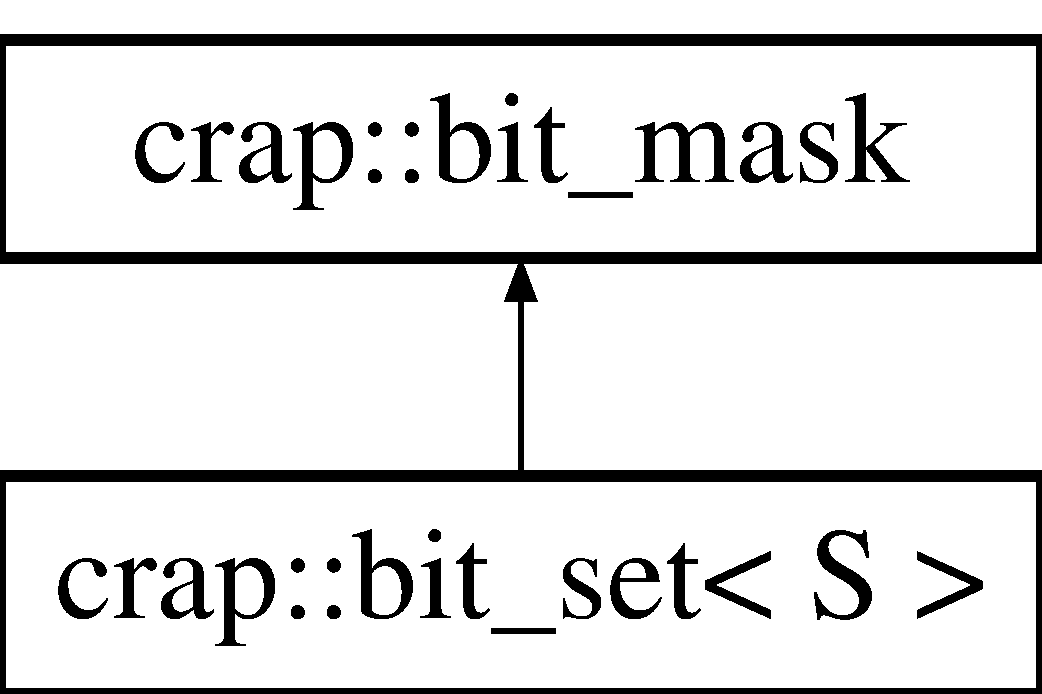
\includegraphics[height=2.000000cm]{classcrap_1_1bit__mask}
\end{center}
\end{figure}
\subsection*{Public Member Functions}
\begin{DoxyCompactItemize}
\item 
\hyperlink{classcrap_1_1bit__mask_a8c61d3022cd0fc1add03ae5d77a428f7}{bit\-\_\-mask} (void)
\begin{DoxyCompactList}\small\item\em Default constructor. \end{DoxyCompactList}\item 
\hyperlink{classcrap_1_1bit__mask_ab42b7bd94645e5df2ca5cee4cd988672}{bit\-\_\-mask} (const \hyperlink{classcrap_1_1bit__mask}{bit\-\_\-mask} \&other)
\begin{DoxyCompactList}\small\item\em Copy constructor. \end{DoxyCompactList}\item 
\hyperlink{classcrap_1_1bit__mask_a2d55cd18751b5b92a7873076feccfb33}{bit\-\_\-mask} (void $\ast$\hyperlink{classcrap_1_1bit__mask_a18d0d45733d73f81f8366e23ca094db4}{pointer}, \hyperlink{types_8h_a38c0a12279ffe0fabec44939e753c914}{size\-\_\-t32} \hyperlink{classcrap_1_1bit__mask_a8bdd624a4eec41c6de938397f67986bd}{size})
\begin{DoxyCompactList}\small\item\em Constructer using parameters for initialization. \end{DoxyCompactList}\item 
\hyperlink{classcrap_1_1bit__mask_ac96ea84ab936e421510763c79f98d7bb}{$\sim$bit\-\_\-mask} (void)
\begin{DoxyCompactList}\small\item\em Destructor. \end{DoxyCompactList}\item 
void \hyperlink{classcrap_1_1bit__mask_adfb7e56b1c5f47ff651c765bee305299}{init} (void $\ast$\hyperlink{classcrap_1_1bit__mask_a18d0d45733d73f81f8366e23ca094db4}{pointer}, \hyperlink{types_8h_a38c0a12279ffe0fabec44939e753c914}{size\-\_\-t32} \hyperlink{classcrap_1_1bit__mask_a8bdd624a4eec41c6de938397f67986bd}{size})
\begin{DoxyCompactList}\small\item\em Initialization. \end{DoxyCompactList}\item 
\hyperlink{classcrap_1_1bit__mask}{bit\-\_\-mask} \& \hyperlink{classcrap_1_1bit__mask_a3cb8adeeedab783e54e8da45633fb0af}{operator=} (const \hyperlink{classcrap_1_1bit__mask}{bit\-\_\-mask} \&other)
\begin{DoxyCompactList}\small\item\em Assignment operator. \end{DoxyCompactList}\item 
\hyperlink{classcrap_1_1bit__mask}{bit\-\_\-mask} \& \hyperlink{classcrap_1_1bit__mask_a8016eccdef681ee9190740e9afcfec08}{operator=} (void $\ast$other)
\begin{DoxyCompactList}\small\item\em Assignment operator -\/ using void pointer and old size. \end{DoxyCompactList}\item 
\hyperlink{classcrap_1_1bit__mask}{bit\-\_\-mask} \& \hyperlink{classcrap_1_1bit__mask_ac9f560b976b5adb616f4c542f4bad7af}{operator+=} (const \hyperlink{classcrap_1_1bit__mask}{bit\-\_\-mask} \&other)
\begin{DoxyCompactList}\small\item\em Plus equal operator. \end{DoxyCompactList}\item 
\hyperlink{classcrap_1_1bit__mask}{bit\-\_\-mask} \& \hyperlink{classcrap_1_1bit__mask_a4b04d247cde37c205ebd1e2d33bcd7c6}{operator+=} (void $\ast$other)
\begin{DoxyCompactList}\small\item\em Plus equal operator -\/ using void pointer and old size. \end{DoxyCompactList}\item 
\hyperlink{classcrap_1_1bit__mask}{bit\-\_\-mask} \& \hyperlink{classcrap_1_1bit__mask_a3b2d989f4ebcbbe605a1b9630aa5f4fe}{operator-\/=} (const \hyperlink{classcrap_1_1bit__mask}{bit\-\_\-mask} \&other)
\begin{DoxyCompactList}\small\item\em Minus equal operator. \end{DoxyCompactList}\item 
\hyperlink{classcrap_1_1bit__mask}{bit\-\_\-mask} \& \hyperlink{classcrap_1_1bit__mask_a74ed54d678c71941a2e070a04d46c0a9}{operator-\/=} (void $\ast$other)
\begin{DoxyCompactList}\small\item\em Minus equal operator -\/ using void pointer and old size. \end{DoxyCompactList}\item 
bool \hyperlink{classcrap_1_1bit__mask_a9dbab8eb36612aceffd9e9d15255f473}{operator==} (const \hyperlink{classcrap_1_1bit__mask}{bit\-\_\-mask} \&other) const 
\begin{DoxyCompactList}\small\item\em Comparision operator. \end{DoxyCompactList}\item 
bool \hyperlink{classcrap_1_1bit__mask_a170b6b81249745c6ea138bdfefec0579}{operator==} (void $\ast$other) const 
\begin{DoxyCompactList}\small\item\em Comparision operator -\/ using void pointer and old size. \end{DoxyCompactList}\item 
bool \hyperlink{classcrap_1_1bit__mask_a123922907c5a811b6c72839982f4a88d}{operator\mbox{[}$\,$\mbox{]}} (\hyperlink{types_8h_a38c0a12279ffe0fabec44939e753c914}{size\-\_\-t32} position) const 
\begin{DoxyCompactList}\small\item\em Accessor on certain bit. \end{DoxyCompactList}\item 
bool \hyperlink{classcrap_1_1bit__mask_afbe08785cec2fe70dec9fb81a485708c}{test} (void) const 
\begin{DoxyCompactList}\small\item\em Test if all bits are set. \end{DoxyCompactList}\item 
bool \hyperlink{classcrap_1_1bit__mask_a29f671c2e98e867c4afe0c08c8223ea4}{test} (\hyperlink{types_8h_a38c0a12279ffe0fabec44939e753c914}{size\-\_\-t32} position) const 
\begin{DoxyCompactList}\small\item\em Test if certain bit is set. \end{DoxyCompactList}\item 
bool \hyperlink{classcrap_1_1bit__mask_ad7562e10c60d4200f56f985667a3d8ff}{test} (\hyperlink{types_8h_a38c0a12279ffe0fabec44939e753c914}{size\-\_\-t32} position, \hyperlink{types_8h_a38c0a12279ffe0fabec44939e753c914}{size\-\_\-t32} lenght) const 
\begin{DoxyCompactList}\small\item\em Test if a sequence of bits is set, lenght as number of bits. \end{DoxyCompactList}\item 
void \hyperlink{classcrap_1_1bit__mask_aa76876c740b0dcff787e585132b50a50}{set} (void)
\begin{DoxyCompactList}\small\item\em Set all bits. \end{DoxyCompactList}\item 
void \hyperlink{classcrap_1_1bit__mask_a9f95a363169039cdb533c181d85bc49b}{set} (\hyperlink{types_8h_a38c0a12279ffe0fabec44939e753c914}{size\-\_\-t32} position)
\begin{DoxyCompactList}\small\item\em Set certain bit. \end{DoxyCompactList}\item 
void \hyperlink{classcrap_1_1bit__mask_ac2828001b93909ba2b06fc6b07adb80b}{set} (\hyperlink{types_8h_a38c0a12279ffe0fabec44939e753c914}{size\-\_\-t32} position, \hyperlink{types_8h_a38c0a12279ffe0fabec44939e753c914}{size\-\_\-t32} lenght)
\begin{DoxyCompactList}\small\item\em Set a sequence of bits. \end{DoxyCompactList}\item 
void \hyperlink{classcrap_1_1bit__mask_a9d7b377eb7d3670b0e963cd52497f7d1}{reset} (void)
\begin{DoxyCompactList}\small\item\em Reset all bits. \end{DoxyCompactList}\item 
void \hyperlink{classcrap_1_1bit__mask_af50dad3c4821620d5687e872bb8bdcbe}{reset} (\hyperlink{types_8h_a38c0a12279ffe0fabec44939e753c914}{size\-\_\-t32} position)
\begin{DoxyCompactList}\small\item\em Reset certain bit. \end{DoxyCompactList}\item 
void \hyperlink{classcrap_1_1bit__mask_acf56c913e8affc9bf2399e03fff62ef5}{reset} (\hyperlink{types_8h_a38c0a12279ffe0fabec44939e753c914}{size\-\_\-t32} from, \hyperlink{types_8h_a38c0a12279ffe0fabec44939e753c914}{size\-\_\-t32} to)
\begin{DoxyCompactList}\small\item\em Reset a sequence of bits. \end{DoxyCompactList}\item 
void \hyperlink{classcrap_1_1bit__mask_acf780848977ef45517e0ecc5063d5231}{flip} (void)
\begin{DoxyCompactList}\small\item\em Flip all bits. \end{DoxyCompactList}\item 
void \hyperlink{classcrap_1_1bit__mask_a6d34bf0c472f5547febefcf68baab095}{flip} (\hyperlink{types_8h_a38c0a12279ffe0fabec44939e753c914}{size\-\_\-t32} position)
\begin{DoxyCompactList}\small\item\em Flip certain bit. \end{DoxyCompactList}\item 
void \hyperlink{classcrap_1_1bit__mask_ad85ebef206759e296aa8edf5aaf3e6dc}{flip} (\hyperlink{types_8h_a38c0a12279ffe0fabec44939e753c914}{size\-\_\-t32} from, \hyperlink{types_8h_a38c0a12279ffe0fabec44939e753c914}{size\-\_\-t32} to)
\begin{DoxyCompactList}\small\item\em Flip a sequence of bits. \end{DoxyCompactList}\item 
\hyperlink{types_8h_a48d6cd8e4135fb2ff7e7f2dac84089ec}{i32} \hyperlink{classcrap_1_1bit__mask_a66b0dc01729f71652595a5eac12a06c7}{find\-\_\-set} (\hyperlink{types_8h_a38c0a12279ffe0fabec44939e753c914}{size\-\_\-t32} position=0) const 
\begin{DoxyCompactList}\small\item\em Find first set bit from position, returns -\/1 is failed. \end{DoxyCompactList}\item 
\hyperlink{types_8h_a48d6cd8e4135fb2ff7e7f2dac84089ec}{i32} \hyperlink{classcrap_1_1bit__mask_ab964501812761624af1a65df632ad0a1}{find\-\_\-set} (\hyperlink{types_8h_a38c0a12279ffe0fabec44939e753c914}{size\-\_\-t32} from, \hyperlink{types_8h_a38c0a12279ffe0fabec44939e753c914}{size\-\_\-t32} length) const 
\begin{DoxyCompactList}\small\item\em Find first set bit in sequence, returns -\/1 is failed. \end{DoxyCompactList}\item 
\hyperlink{types_8h_a48d6cd8e4135fb2ff7e7f2dac84089ec}{i32} \hyperlink{classcrap_1_1bit__mask_a25921fc85e3f0b8a3b7571863793fb12}{find\-\_\-unset} (\hyperlink{types_8h_a38c0a12279ffe0fabec44939e753c914}{size\-\_\-t32} position=0) const 
\begin{DoxyCompactList}\small\item\em Find first unset bit from position, returns -\/1 is failed. \end{DoxyCompactList}\item 
\hyperlink{types_8h_a48d6cd8e4135fb2ff7e7f2dac84089ec}{i32} \hyperlink{classcrap_1_1bit__mask_a819c2779915ff72df0d9e6e40e0351bd}{find\-\_\-unset} (\hyperlink{types_8h_a38c0a12279ffe0fabec44939e753c914}{size\-\_\-t32} from, \hyperlink{types_8h_a38c0a12279ffe0fabec44939e753c914}{size\-\_\-t32} length) const 
\begin{DoxyCompactList}\small\item\em Find first set bit in sequence, returns -\/1 is failed. \end{DoxyCompactList}\item 
void $\ast$ \hyperlink{classcrap_1_1bit__mask_a18d0d45733d73f81f8366e23ca094db4}{pointer} (void) const 
\begin{DoxyCompactList}\small\item\em Return pointer to memory. \end{DoxyCompactList}\item 
\hyperlink{types_8h_a38c0a12279ffe0fabec44939e753c914}{size\-\_\-t32} \hyperlink{classcrap_1_1bit__mask_a8bdd624a4eec41c6de938397f67986bd}{size} (void) const 
\begin{DoxyCompactList}\small\item\em Return size of manipulated bits. \end{DoxyCompactList}\item 
\hyperlink{types_8h_a38c0a12279ffe0fabec44939e753c914}{size\-\_\-t32} \hyperlink{classcrap_1_1bit__mask_a9848eea9096e1dfd844218f2ddf4ecba}{used\-\_\-bytes} (void) const 
\begin{DoxyCompactList}\small\item\em Return size of manipulated bytes. \end{DoxyCompactList}\end{DoxyCompactItemize}
\subsection*{Protected Attributes}
\begin{DoxyCompactItemize}
\item 
void $\ast$ \hyperlink{classcrap_1_1bit__mask_ae17fa85acdd359a55c29d22e2b0eda06}{\-\_\-pointer}
\item 
\hyperlink{types_8h_a38c0a12279ffe0fabec44939e753c914}{size\-\_\-t32} \hyperlink{classcrap_1_1bit__mask_ae81a3f9f9e8d8bad564985882b1b9a5d}{\-\_\-bits}
\item 
\hyperlink{types_8h_a38c0a12279ffe0fabec44939e753c914}{size\-\_\-t32} \hyperlink{classcrap_1_1bit__mask_ad2e0fc867c1197151d99c1b6b01384aa}{\-\_\-bytes}
\end{DoxyCompactItemize}
\subsection*{Friends}
\begin{DoxyCompactItemize}
\item 
std\-::ostream \& \hyperlink{classcrap_1_1bit__mask_a9022f18a60ecf31fe105c14cd53e6b55}{operator$<$$<$} (std\-::ostream \&out, const \hyperlink{classcrap_1_1bit__mask}{bit\-\_\-mask} \&bitmask)
\begin{DoxyCompactList}\small\item\em Declare stream operator as friend. \end{DoxyCompactList}\end{DoxyCompactItemize}


\subsection{Constructor \& Destructor Documentation}
\hypertarget{classcrap_1_1bit__mask_a8c61d3022cd0fc1add03ae5d77a428f7}{\index{crap\-::bit\-\_\-mask@{crap\-::bit\-\_\-mask}!bit\-\_\-mask@{bit\-\_\-mask}}
\index{bit\-\_\-mask@{bit\-\_\-mask}!crap::bit_mask@{crap\-::bit\-\_\-mask}}
\subsubsection[{bit\-\_\-mask}]{\setlength{\rightskip}{0pt plus 5cm}crap\-::bit\-\_\-mask\-::bit\-\_\-mask (
\begin{DoxyParamCaption}
\item[{void}]{}
\end{DoxyParamCaption}
)}}\label{classcrap_1_1bit__mask_a8c61d3022cd0fc1add03ae5d77a428f7}


Default constructor. 

\hypertarget{classcrap_1_1bit__mask_ab42b7bd94645e5df2ca5cee4cd988672}{\index{crap\-::bit\-\_\-mask@{crap\-::bit\-\_\-mask}!bit\-\_\-mask@{bit\-\_\-mask}}
\index{bit\-\_\-mask@{bit\-\_\-mask}!crap::bit_mask@{crap\-::bit\-\_\-mask}}
\subsubsection[{bit\-\_\-mask}]{\setlength{\rightskip}{0pt plus 5cm}crap\-::bit\-\_\-mask\-::bit\-\_\-mask (
\begin{DoxyParamCaption}
\item[{const {\bf bit\-\_\-mask} \&}]{other}
\end{DoxyParamCaption}
)}}\label{classcrap_1_1bit__mask_ab42b7bd94645e5df2ca5cee4cd988672}


Copy constructor. 

\hypertarget{classcrap_1_1bit__mask_a2d55cd18751b5b92a7873076feccfb33}{\index{crap\-::bit\-\_\-mask@{crap\-::bit\-\_\-mask}!bit\-\_\-mask@{bit\-\_\-mask}}
\index{bit\-\_\-mask@{bit\-\_\-mask}!crap::bit_mask@{crap\-::bit\-\_\-mask}}
\subsubsection[{bit\-\_\-mask}]{\setlength{\rightskip}{0pt plus 5cm}crap\-::bit\-\_\-mask\-::bit\-\_\-mask (
\begin{DoxyParamCaption}
\item[{void $\ast$}]{pointer, }
\item[{{\bf size\-\_\-t32}}]{size}
\end{DoxyParamCaption}
)}}\label{classcrap_1_1bit__mask_a2d55cd18751b5b92a7873076feccfb33}


Constructer using parameters for initialization. 

\hypertarget{classcrap_1_1bit__mask_ac96ea84ab936e421510763c79f98d7bb}{\index{crap\-::bit\-\_\-mask@{crap\-::bit\-\_\-mask}!$\sim$bit\-\_\-mask@{$\sim$bit\-\_\-mask}}
\index{$\sim$bit\-\_\-mask@{$\sim$bit\-\_\-mask}!crap::bit_mask@{crap\-::bit\-\_\-mask}}
\subsubsection[{$\sim$bit\-\_\-mask}]{\setlength{\rightskip}{0pt plus 5cm}crap\-::bit\-\_\-mask\-::$\sim$bit\-\_\-mask (
\begin{DoxyParamCaption}
\item[{void}]{}
\end{DoxyParamCaption}
)}}\label{classcrap_1_1bit__mask_ac96ea84ab936e421510763c79f98d7bb}


Destructor. 



\subsection{Member Function Documentation}
\hypertarget{classcrap_1_1bit__mask_a66b0dc01729f71652595a5eac12a06c7}{\index{crap\-::bit\-\_\-mask@{crap\-::bit\-\_\-mask}!find\-\_\-set@{find\-\_\-set}}
\index{find\-\_\-set@{find\-\_\-set}!crap::bit_mask@{crap\-::bit\-\_\-mask}}
\subsubsection[{find\-\_\-set}]{\setlength{\rightskip}{0pt plus 5cm}{\bf i32} crap\-::bit\-\_\-mask\-::find\-\_\-set (
\begin{DoxyParamCaption}
\item[{{\bf size\-\_\-t32}}]{position = {\ttfamily 0}}
\end{DoxyParamCaption}
) const}}\label{classcrap_1_1bit__mask_a66b0dc01729f71652595a5eac12a06c7}


Find first set bit from position, returns -\/1 is failed. 

\hypertarget{classcrap_1_1bit__mask_ab964501812761624af1a65df632ad0a1}{\index{crap\-::bit\-\_\-mask@{crap\-::bit\-\_\-mask}!find\-\_\-set@{find\-\_\-set}}
\index{find\-\_\-set@{find\-\_\-set}!crap::bit_mask@{crap\-::bit\-\_\-mask}}
\subsubsection[{find\-\_\-set}]{\setlength{\rightskip}{0pt plus 5cm}{\bf i32} crap\-::bit\-\_\-mask\-::find\-\_\-set (
\begin{DoxyParamCaption}
\item[{{\bf size\-\_\-t32}}]{from, }
\item[{{\bf size\-\_\-t32}}]{length}
\end{DoxyParamCaption}
) const}}\label{classcrap_1_1bit__mask_ab964501812761624af1a65df632ad0a1}


Find first set bit in sequence, returns -\/1 is failed. 

\hypertarget{classcrap_1_1bit__mask_a25921fc85e3f0b8a3b7571863793fb12}{\index{crap\-::bit\-\_\-mask@{crap\-::bit\-\_\-mask}!find\-\_\-unset@{find\-\_\-unset}}
\index{find\-\_\-unset@{find\-\_\-unset}!crap::bit_mask@{crap\-::bit\-\_\-mask}}
\subsubsection[{find\-\_\-unset}]{\setlength{\rightskip}{0pt plus 5cm}{\bf i32} crap\-::bit\-\_\-mask\-::find\-\_\-unset (
\begin{DoxyParamCaption}
\item[{{\bf size\-\_\-t32}}]{position = {\ttfamily 0}}
\end{DoxyParamCaption}
) const}}\label{classcrap_1_1bit__mask_a25921fc85e3f0b8a3b7571863793fb12}


Find first unset bit from position, returns -\/1 is failed. 

\hypertarget{classcrap_1_1bit__mask_a819c2779915ff72df0d9e6e40e0351bd}{\index{crap\-::bit\-\_\-mask@{crap\-::bit\-\_\-mask}!find\-\_\-unset@{find\-\_\-unset}}
\index{find\-\_\-unset@{find\-\_\-unset}!crap::bit_mask@{crap\-::bit\-\_\-mask}}
\subsubsection[{find\-\_\-unset}]{\setlength{\rightskip}{0pt plus 5cm}{\bf i32} crap\-::bit\-\_\-mask\-::find\-\_\-unset (
\begin{DoxyParamCaption}
\item[{{\bf size\-\_\-t32}}]{from, }
\item[{{\bf size\-\_\-t32}}]{length}
\end{DoxyParamCaption}
) const}}\label{classcrap_1_1bit__mask_a819c2779915ff72df0d9e6e40e0351bd}


Find first set bit in sequence, returns -\/1 is failed. 

\hypertarget{classcrap_1_1bit__mask_acf780848977ef45517e0ecc5063d5231}{\index{crap\-::bit\-\_\-mask@{crap\-::bit\-\_\-mask}!flip@{flip}}
\index{flip@{flip}!crap::bit_mask@{crap\-::bit\-\_\-mask}}
\subsubsection[{flip}]{\setlength{\rightskip}{0pt plus 5cm}void crap\-::bit\-\_\-mask\-::flip (
\begin{DoxyParamCaption}
\item[{void}]{}
\end{DoxyParamCaption}
)}}\label{classcrap_1_1bit__mask_acf780848977ef45517e0ecc5063d5231}


Flip all bits. 

\hypertarget{classcrap_1_1bit__mask_a6d34bf0c472f5547febefcf68baab095}{\index{crap\-::bit\-\_\-mask@{crap\-::bit\-\_\-mask}!flip@{flip}}
\index{flip@{flip}!crap::bit_mask@{crap\-::bit\-\_\-mask}}
\subsubsection[{flip}]{\setlength{\rightskip}{0pt plus 5cm}void crap\-::bit\-\_\-mask\-::flip (
\begin{DoxyParamCaption}
\item[{{\bf size\-\_\-t32}}]{position}
\end{DoxyParamCaption}
)}}\label{classcrap_1_1bit__mask_a6d34bf0c472f5547febefcf68baab095}


Flip certain bit. 

\hypertarget{classcrap_1_1bit__mask_ad85ebef206759e296aa8edf5aaf3e6dc}{\index{crap\-::bit\-\_\-mask@{crap\-::bit\-\_\-mask}!flip@{flip}}
\index{flip@{flip}!crap::bit_mask@{crap\-::bit\-\_\-mask}}
\subsubsection[{flip}]{\setlength{\rightskip}{0pt plus 5cm}void crap\-::bit\-\_\-mask\-::flip (
\begin{DoxyParamCaption}
\item[{{\bf size\-\_\-t32}}]{from, }
\item[{{\bf size\-\_\-t32}}]{to}
\end{DoxyParamCaption}
)}}\label{classcrap_1_1bit__mask_ad85ebef206759e296aa8edf5aaf3e6dc}


Flip a sequence of bits. 

\hypertarget{classcrap_1_1bit__mask_adfb7e56b1c5f47ff651c765bee305299}{\index{crap\-::bit\-\_\-mask@{crap\-::bit\-\_\-mask}!init@{init}}
\index{init@{init}!crap::bit_mask@{crap\-::bit\-\_\-mask}}
\subsubsection[{init}]{\setlength{\rightskip}{0pt plus 5cm}void crap\-::bit\-\_\-mask\-::init (
\begin{DoxyParamCaption}
\item[{void $\ast$}]{pointer, }
\item[{{\bf size\-\_\-t32}}]{size}
\end{DoxyParamCaption}
)}}\label{classcrap_1_1bit__mask_adfb7e56b1c5f47ff651c765bee305299}


Initialization. 

\hypertarget{classcrap_1_1bit__mask_ac9f560b976b5adb616f4c542f4bad7af}{\index{crap\-::bit\-\_\-mask@{crap\-::bit\-\_\-mask}!operator+=@{operator+=}}
\index{operator+=@{operator+=}!crap::bit_mask@{crap\-::bit\-\_\-mask}}
\subsubsection[{operator+=}]{\setlength{\rightskip}{0pt plus 5cm}{\bf bit\-\_\-mask} \& crap\-::bit\-\_\-mask\-::operator+= (
\begin{DoxyParamCaption}
\item[{const {\bf bit\-\_\-mask} \&}]{other}
\end{DoxyParamCaption}
)}}\label{classcrap_1_1bit__mask_ac9f560b976b5adb616f4c542f4bad7af}


Plus equal operator. 

\hypertarget{classcrap_1_1bit__mask_a4b04d247cde37c205ebd1e2d33bcd7c6}{\index{crap\-::bit\-\_\-mask@{crap\-::bit\-\_\-mask}!operator+=@{operator+=}}
\index{operator+=@{operator+=}!crap::bit_mask@{crap\-::bit\-\_\-mask}}
\subsubsection[{operator+=}]{\setlength{\rightskip}{0pt plus 5cm}{\bf bit\-\_\-mask} \& crap\-::bit\-\_\-mask\-::operator+= (
\begin{DoxyParamCaption}
\item[{void $\ast$}]{other}
\end{DoxyParamCaption}
)}}\label{classcrap_1_1bit__mask_a4b04d247cde37c205ebd1e2d33bcd7c6}


Plus equal operator -\/ using void pointer and old size. 

\hypertarget{classcrap_1_1bit__mask_a3b2d989f4ebcbbe605a1b9630aa5f4fe}{\index{crap\-::bit\-\_\-mask@{crap\-::bit\-\_\-mask}!operator-\/=@{operator-\/=}}
\index{operator-\/=@{operator-\/=}!crap::bit_mask@{crap\-::bit\-\_\-mask}}
\subsubsection[{operator-\/=}]{\setlength{\rightskip}{0pt plus 5cm}{\bf bit\-\_\-mask} \& crap\-::bit\-\_\-mask\-::operator-\/= (
\begin{DoxyParamCaption}
\item[{const {\bf bit\-\_\-mask} \&}]{other}
\end{DoxyParamCaption}
)}}\label{classcrap_1_1bit__mask_a3b2d989f4ebcbbe605a1b9630aa5f4fe}


Minus equal operator. 

\hypertarget{classcrap_1_1bit__mask_a74ed54d678c71941a2e070a04d46c0a9}{\index{crap\-::bit\-\_\-mask@{crap\-::bit\-\_\-mask}!operator-\/=@{operator-\/=}}
\index{operator-\/=@{operator-\/=}!crap::bit_mask@{crap\-::bit\-\_\-mask}}
\subsubsection[{operator-\/=}]{\setlength{\rightskip}{0pt plus 5cm}{\bf bit\-\_\-mask} \& crap\-::bit\-\_\-mask\-::operator-\/= (
\begin{DoxyParamCaption}
\item[{void $\ast$}]{other}
\end{DoxyParamCaption}
)}}\label{classcrap_1_1bit__mask_a74ed54d678c71941a2e070a04d46c0a9}


Minus equal operator -\/ using void pointer and old size. 

\hypertarget{classcrap_1_1bit__mask_a3cb8adeeedab783e54e8da45633fb0af}{\index{crap\-::bit\-\_\-mask@{crap\-::bit\-\_\-mask}!operator=@{operator=}}
\index{operator=@{operator=}!crap::bit_mask@{crap\-::bit\-\_\-mask}}
\subsubsection[{operator=}]{\setlength{\rightskip}{0pt plus 5cm}{\bf bit\-\_\-mask} \& crap\-::bit\-\_\-mask\-::operator= (
\begin{DoxyParamCaption}
\item[{const {\bf bit\-\_\-mask} \&}]{other}
\end{DoxyParamCaption}
)}}\label{classcrap_1_1bit__mask_a3cb8adeeedab783e54e8da45633fb0af}


Assignment operator. 

\hypertarget{classcrap_1_1bit__mask_a8016eccdef681ee9190740e9afcfec08}{\index{crap\-::bit\-\_\-mask@{crap\-::bit\-\_\-mask}!operator=@{operator=}}
\index{operator=@{operator=}!crap::bit_mask@{crap\-::bit\-\_\-mask}}
\subsubsection[{operator=}]{\setlength{\rightskip}{0pt plus 5cm}{\bf bit\-\_\-mask} \& crap\-::bit\-\_\-mask\-::operator= (
\begin{DoxyParamCaption}
\item[{void $\ast$}]{other}
\end{DoxyParamCaption}
)}}\label{classcrap_1_1bit__mask_a8016eccdef681ee9190740e9afcfec08}


Assignment operator -\/ using void pointer and old size. 

\hypertarget{classcrap_1_1bit__mask_a9dbab8eb36612aceffd9e9d15255f473}{\index{crap\-::bit\-\_\-mask@{crap\-::bit\-\_\-mask}!operator==@{operator==}}
\index{operator==@{operator==}!crap::bit_mask@{crap\-::bit\-\_\-mask}}
\subsubsection[{operator==}]{\setlength{\rightskip}{0pt plus 5cm}bool crap\-::bit\-\_\-mask\-::operator== (
\begin{DoxyParamCaption}
\item[{const {\bf bit\-\_\-mask} \&}]{other}
\end{DoxyParamCaption}
) const}}\label{classcrap_1_1bit__mask_a9dbab8eb36612aceffd9e9d15255f473}


Comparision operator. 

\hypertarget{classcrap_1_1bit__mask_a170b6b81249745c6ea138bdfefec0579}{\index{crap\-::bit\-\_\-mask@{crap\-::bit\-\_\-mask}!operator==@{operator==}}
\index{operator==@{operator==}!crap::bit_mask@{crap\-::bit\-\_\-mask}}
\subsubsection[{operator==}]{\setlength{\rightskip}{0pt plus 5cm}bool crap\-::bit\-\_\-mask\-::operator== (
\begin{DoxyParamCaption}
\item[{void $\ast$}]{other}
\end{DoxyParamCaption}
) const}}\label{classcrap_1_1bit__mask_a170b6b81249745c6ea138bdfefec0579}


Comparision operator -\/ using void pointer and old size. 

\hypertarget{classcrap_1_1bit__mask_a123922907c5a811b6c72839982f4a88d}{\index{crap\-::bit\-\_\-mask@{crap\-::bit\-\_\-mask}!operator\mbox{[}$\,$\mbox{]}@{operator[]}}
\index{operator\mbox{[}$\,$\mbox{]}@{operator[]}!crap::bit_mask@{crap\-::bit\-\_\-mask}}
\subsubsection[{operator[]}]{\setlength{\rightskip}{0pt plus 5cm}bool crap\-::bit\-\_\-mask\-::operator\mbox{[}$\,$\mbox{]} (
\begin{DoxyParamCaption}
\item[{{\bf size\-\_\-t32}}]{position}
\end{DoxyParamCaption}
) const}}\label{classcrap_1_1bit__mask_a123922907c5a811b6c72839982f4a88d}


Accessor on certain bit. 

\hypertarget{classcrap_1_1bit__mask_a18d0d45733d73f81f8366e23ca094db4}{\index{crap\-::bit\-\_\-mask@{crap\-::bit\-\_\-mask}!pointer@{pointer}}
\index{pointer@{pointer}!crap::bit_mask@{crap\-::bit\-\_\-mask}}
\subsubsection[{pointer}]{\setlength{\rightskip}{0pt plus 5cm}void $\ast$ crap\-::bit\-\_\-mask\-::pointer (
\begin{DoxyParamCaption}
\item[{void}]{}
\end{DoxyParamCaption}
) const}}\label{classcrap_1_1bit__mask_a18d0d45733d73f81f8366e23ca094db4}


Return pointer to memory. 

\hypertarget{classcrap_1_1bit__mask_a9d7b377eb7d3670b0e963cd52497f7d1}{\index{crap\-::bit\-\_\-mask@{crap\-::bit\-\_\-mask}!reset@{reset}}
\index{reset@{reset}!crap::bit_mask@{crap\-::bit\-\_\-mask}}
\subsubsection[{reset}]{\setlength{\rightskip}{0pt plus 5cm}void crap\-::bit\-\_\-mask\-::reset (
\begin{DoxyParamCaption}
\item[{void}]{}
\end{DoxyParamCaption}
)}}\label{classcrap_1_1bit__mask_a9d7b377eb7d3670b0e963cd52497f7d1}


Reset all bits. 

\hypertarget{classcrap_1_1bit__mask_af50dad3c4821620d5687e872bb8bdcbe}{\index{crap\-::bit\-\_\-mask@{crap\-::bit\-\_\-mask}!reset@{reset}}
\index{reset@{reset}!crap::bit_mask@{crap\-::bit\-\_\-mask}}
\subsubsection[{reset}]{\setlength{\rightskip}{0pt plus 5cm}void crap\-::bit\-\_\-mask\-::reset (
\begin{DoxyParamCaption}
\item[{{\bf size\-\_\-t32}}]{position}
\end{DoxyParamCaption}
)}}\label{classcrap_1_1bit__mask_af50dad3c4821620d5687e872bb8bdcbe}


Reset certain bit. 

\hypertarget{classcrap_1_1bit__mask_acf56c913e8affc9bf2399e03fff62ef5}{\index{crap\-::bit\-\_\-mask@{crap\-::bit\-\_\-mask}!reset@{reset}}
\index{reset@{reset}!crap::bit_mask@{crap\-::bit\-\_\-mask}}
\subsubsection[{reset}]{\setlength{\rightskip}{0pt plus 5cm}void crap\-::bit\-\_\-mask\-::reset (
\begin{DoxyParamCaption}
\item[{{\bf size\-\_\-t32}}]{from, }
\item[{{\bf size\-\_\-t32}}]{to}
\end{DoxyParamCaption}
)}}\label{classcrap_1_1bit__mask_acf56c913e8affc9bf2399e03fff62ef5}


Reset a sequence of bits. 

\hypertarget{classcrap_1_1bit__mask_aa76876c740b0dcff787e585132b50a50}{\index{crap\-::bit\-\_\-mask@{crap\-::bit\-\_\-mask}!set@{set}}
\index{set@{set}!crap::bit_mask@{crap\-::bit\-\_\-mask}}
\subsubsection[{set}]{\setlength{\rightskip}{0pt plus 5cm}void crap\-::bit\-\_\-mask\-::set (
\begin{DoxyParamCaption}
\item[{void}]{}
\end{DoxyParamCaption}
)}}\label{classcrap_1_1bit__mask_aa76876c740b0dcff787e585132b50a50}


Set all bits. 

\hypertarget{classcrap_1_1bit__mask_a9f95a363169039cdb533c181d85bc49b}{\index{crap\-::bit\-\_\-mask@{crap\-::bit\-\_\-mask}!set@{set}}
\index{set@{set}!crap::bit_mask@{crap\-::bit\-\_\-mask}}
\subsubsection[{set}]{\setlength{\rightskip}{0pt plus 5cm}void crap\-::bit\-\_\-mask\-::set (
\begin{DoxyParamCaption}
\item[{{\bf size\-\_\-t32}}]{position}
\end{DoxyParamCaption}
)}}\label{classcrap_1_1bit__mask_a9f95a363169039cdb533c181d85bc49b}


Set certain bit. 

\hypertarget{classcrap_1_1bit__mask_ac2828001b93909ba2b06fc6b07adb80b}{\index{crap\-::bit\-\_\-mask@{crap\-::bit\-\_\-mask}!set@{set}}
\index{set@{set}!crap::bit_mask@{crap\-::bit\-\_\-mask}}
\subsubsection[{set}]{\setlength{\rightskip}{0pt plus 5cm}void crap\-::bit\-\_\-mask\-::set (
\begin{DoxyParamCaption}
\item[{{\bf size\-\_\-t32}}]{position, }
\item[{{\bf size\-\_\-t32}}]{lenght}
\end{DoxyParamCaption}
)}}\label{classcrap_1_1bit__mask_ac2828001b93909ba2b06fc6b07adb80b}


Set a sequence of bits. 

\hypertarget{classcrap_1_1bit__mask_a8bdd624a4eec41c6de938397f67986bd}{\index{crap\-::bit\-\_\-mask@{crap\-::bit\-\_\-mask}!size@{size}}
\index{size@{size}!crap::bit_mask@{crap\-::bit\-\_\-mask}}
\subsubsection[{size}]{\setlength{\rightskip}{0pt plus 5cm}{\bf size\-\_\-t32} crap\-::bit\-\_\-mask\-::size (
\begin{DoxyParamCaption}
\item[{void}]{}
\end{DoxyParamCaption}
) const}}\label{classcrap_1_1bit__mask_a8bdd624a4eec41c6de938397f67986bd}


Return size of manipulated bits. 

\hypertarget{classcrap_1_1bit__mask_afbe08785cec2fe70dec9fb81a485708c}{\index{crap\-::bit\-\_\-mask@{crap\-::bit\-\_\-mask}!test@{test}}
\index{test@{test}!crap::bit_mask@{crap\-::bit\-\_\-mask}}
\subsubsection[{test}]{\setlength{\rightskip}{0pt plus 5cm}bool crap\-::bit\-\_\-mask\-::test (
\begin{DoxyParamCaption}
\item[{void}]{}
\end{DoxyParamCaption}
) const}}\label{classcrap_1_1bit__mask_afbe08785cec2fe70dec9fb81a485708c}


Test if all bits are set. 

\hypertarget{classcrap_1_1bit__mask_a29f671c2e98e867c4afe0c08c8223ea4}{\index{crap\-::bit\-\_\-mask@{crap\-::bit\-\_\-mask}!test@{test}}
\index{test@{test}!crap::bit_mask@{crap\-::bit\-\_\-mask}}
\subsubsection[{test}]{\setlength{\rightskip}{0pt plus 5cm}bool crap\-::bit\-\_\-mask\-::test (
\begin{DoxyParamCaption}
\item[{{\bf size\-\_\-t32}}]{position}
\end{DoxyParamCaption}
) const}}\label{classcrap_1_1bit__mask_a29f671c2e98e867c4afe0c08c8223ea4}


Test if certain bit is set. 

\hypertarget{classcrap_1_1bit__mask_ad7562e10c60d4200f56f985667a3d8ff}{\index{crap\-::bit\-\_\-mask@{crap\-::bit\-\_\-mask}!test@{test}}
\index{test@{test}!crap::bit_mask@{crap\-::bit\-\_\-mask}}
\subsubsection[{test}]{\setlength{\rightskip}{0pt plus 5cm}bool crap\-::bit\-\_\-mask\-::test (
\begin{DoxyParamCaption}
\item[{{\bf size\-\_\-t32}}]{position, }
\item[{{\bf size\-\_\-t32}}]{lenght}
\end{DoxyParamCaption}
) const}}\label{classcrap_1_1bit__mask_ad7562e10c60d4200f56f985667a3d8ff}


Test if a sequence of bits is set, lenght as number of bits. 

\hypertarget{classcrap_1_1bit__mask_a9848eea9096e1dfd844218f2ddf4ecba}{\index{crap\-::bit\-\_\-mask@{crap\-::bit\-\_\-mask}!used\-\_\-bytes@{used\-\_\-bytes}}
\index{used\-\_\-bytes@{used\-\_\-bytes}!crap::bit_mask@{crap\-::bit\-\_\-mask}}
\subsubsection[{used\-\_\-bytes}]{\setlength{\rightskip}{0pt plus 5cm}{\bf size\-\_\-t32} crap\-::bit\-\_\-mask\-::used\-\_\-bytes (
\begin{DoxyParamCaption}
\item[{void}]{}
\end{DoxyParamCaption}
) const}}\label{classcrap_1_1bit__mask_a9848eea9096e1dfd844218f2ddf4ecba}


Return size of manipulated bytes. 



\subsection{Friends And Related Function Documentation}
\hypertarget{classcrap_1_1bit__mask_a9022f18a60ecf31fe105c14cd53e6b55}{\index{crap\-::bit\-\_\-mask@{crap\-::bit\-\_\-mask}!operator$<$$<$@{operator$<$$<$}}
\index{operator$<$$<$@{operator$<$$<$}!crap::bit_mask@{crap\-::bit\-\_\-mask}}
\subsubsection[{operator$<$$<$}]{\setlength{\rightskip}{0pt plus 5cm}std\-::ostream\& operator$<$$<$ (
\begin{DoxyParamCaption}
\item[{std\-::ostream \&}]{out, }
\item[{const {\bf bit\-\_\-mask} \&}]{bitmask}
\end{DoxyParamCaption}
)\hspace{0.3cm}{\ttfamily [friend]}}}\label{classcrap_1_1bit__mask_a9022f18a60ecf31fe105c14cd53e6b55}


Declare stream operator as friend. 



\subsection{Member Data Documentation}
\hypertarget{classcrap_1_1bit__mask_ae81a3f9f9e8d8bad564985882b1b9a5d}{\index{crap\-::bit\-\_\-mask@{crap\-::bit\-\_\-mask}!\-\_\-bits@{\-\_\-bits}}
\index{\-\_\-bits@{\-\_\-bits}!crap::bit_mask@{crap\-::bit\-\_\-mask}}
\subsubsection[{\-\_\-bits}]{\setlength{\rightskip}{0pt plus 5cm}{\bf size\-\_\-t32} crap\-::bit\-\_\-mask\-::\-\_\-bits\hspace{0.3cm}{\ttfamily [protected]}}}\label{classcrap_1_1bit__mask_ae81a3f9f9e8d8bad564985882b1b9a5d}
\hypertarget{classcrap_1_1bit__mask_ad2e0fc867c1197151d99c1b6b01384aa}{\index{crap\-::bit\-\_\-mask@{crap\-::bit\-\_\-mask}!\-\_\-bytes@{\-\_\-bytes}}
\index{\-\_\-bytes@{\-\_\-bytes}!crap::bit_mask@{crap\-::bit\-\_\-mask}}
\subsubsection[{\-\_\-bytes}]{\setlength{\rightskip}{0pt plus 5cm}{\bf size\-\_\-t32} crap\-::bit\-\_\-mask\-::\-\_\-bytes\hspace{0.3cm}{\ttfamily [protected]}}}\label{classcrap_1_1bit__mask_ad2e0fc867c1197151d99c1b6b01384aa}
\hypertarget{classcrap_1_1bit__mask_ae17fa85acdd359a55c29d22e2b0eda06}{\index{crap\-::bit\-\_\-mask@{crap\-::bit\-\_\-mask}!\-\_\-pointer@{\-\_\-pointer}}
\index{\-\_\-pointer@{\-\_\-pointer}!crap::bit_mask@{crap\-::bit\-\_\-mask}}
\subsubsection[{\-\_\-pointer}]{\setlength{\rightskip}{0pt plus 5cm}void$\ast$ crap\-::bit\-\_\-mask\-::\-\_\-pointer\hspace{0.3cm}{\ttfamily [protected]}}}\label{classcrap_1_1bit__mask_ae17fa85acdd359a55c29d22e2b0eda06}


The documentation for this class was generated from the following files\-:\begin{DoxyCompactItemize}
\item 
/mnt/windows/data/\-Programmierung/\-C\-R\-A\-P/src/crap/container/\hyperlink{bitmask_8h}{bitmask.\-h}\item 
/mnt/windows/data/\-Programmierung/\-C\-R\-A\-P/src/crap/container/\hyperlink{bitmask_8cpp}{bitmask.\-cpp}\end{DoxyCompactItemize}

\hypertarget{classcrap_1_1bit__set}{\section{crap\-:\-:bit\-\_\-set$<$ S $>$ Class Template Reference}
\label{classcrap_1_1bit__set}\index{crap\-::bit\-\_\-set$<$ S $>$@{crap\-::bit\-\_\-set$<$ S $>$}}
}


{\ttfamily \#include $<$bitset.\-h$>$}

Inheritance diagram for crap\-:\-:bit\-\_\-set$<$ S $>$\-:\begin{figure}[H]
\begin{center}
\leavevmode
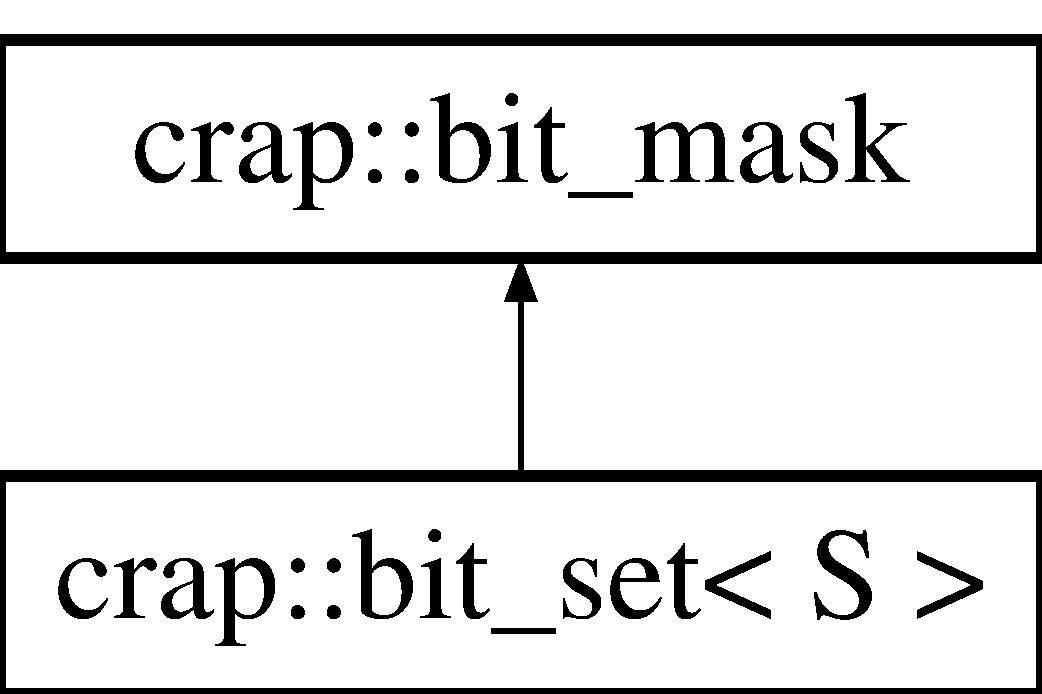
\includegraphics[height=2.000000cm]{classcrap_1_1bit__set}
\end{center}
\end{figure}
\subsection*{Public Member Functions}
\begin{DoxyCompactItemize}
\item 
\hyperlink{classcrap_1_1bit__set_a637e5ed9347b437f4931d47ea7197789}{bit\-\_\-set} (void)
\begin{DoxyCompactList}\small\item\em default constructor \end{DoxyCompactList}\item 
\hyperlink{classcrap_1_1bit__set_a08a9c32a0783390cb10095b2eb1637ec}{bit\-\_\-set} (const \hyperlink{classcrap_1_1bit__set}{bit\-\_\-set} \&other)
\begin{DoxyCompactList}\small\item\em copy constructor \end{DoxyCompactList}\item 
\hyperlink{classcrap_1_1bit__set_ac6c26b4d5a554c1ebb55e65d4aa9dc62}{$\sim$bit\-\_\-set} (void)
\begin{DoxyCompactList}\small\item\em destructor \end{DoxyCompactList}\item 
\hyperlink{classcrap_1_1bit__set}{bit\-\_\-set} \& \hyperlink{classcrap_1_1bit__set_a8e17967e278f7dfe9ae336c0efb3d82c}{operator=} (const \hyperlink{classcrap_1_1bit__set}{bit\-\_\-set} \&other)
\begin{DoxyCompactList}\small\item\em assignment operator \end{DoxyCompactList}\item 
\hyperlink{classcrap_1_1bit__set}{bit\-\_\-set} \& \hyperlink{classcrap_1_1bit__set_a2ae2bd31cb1c618a657ab2fb266633c0}{operator=} (void $\ast$other)
\begin{DoxyCompactList}\small\item\em assignment operator with pointer \end{DoxyCompactList}\item 
\hyperlink{classcrap_1_1bit__set}{bit\-\_\-set} \& \hyperlink{classcrap_1_1bit__set_ad15d347927bf719d2ede49730ecdc941}{operator+=} (const \hyperlink{classcrap_1_1bit__set}{bit\-\_\-set} \&other)
\begin{DoxyCompactList}\small\item\em plus-\/equal operator \end{DoxyCompactList}\item 
\hyperlink{classcrap_1_1bit__set}{bit\-\_\-set} \& \hyperlink{classcrap_1_1bit__set_a59067fd5e5ebfe0e01fc459f0420e3b6}{operator+=} (void $\ast$other)
\begin{DoxyCompactList}\small\item\em plus-\/equal operator with pointer \end{DoxyCompactList}\item 
\hyperlink{classcrap_1_1bit__set}{bit\-\_\-set} \& \hyperlink{classcrap_1_1bit__set_afcfd210f22043f918f75e69253114106}{operator-\/=} (const \hyperlink{classcrap_1_1bit__set}{bit\-\_\-set} \&other)
\begin{DoxyCompactList}\small\item\em minus-\/equal operator \end{DoxyCompactList}\item 
\hyperlink{classcrap_1_1bit__set}{bit\-\_\-set} \& \hyperlink{classcrap_1_1bit__set_a67748b5ee0f8167126ce8d54736ec57d}{operator-\/=} (void $\ast$other)
\begin{DoxyCompactList}\small\item\em minus-\/equal operator with pointer \end{DoxyCompactList}\end{DoxyCompactItemize}
\subsection*{Friends}
\begin{DoxyCompactItemize}
\item 
{\footnotesize template$<$size\-\_\-t32 U$>$ }\\std\-::ostream \& \hyperlink{classcrap_1_1bit__set_a0b8ecaed0455cc93e7f32f14d08f391f}{operator$<$$<$} (std\-::ostream \&out, const \hyperlink{classcrap_1_1bit__set}{bit\-\_\-set}$<$ U $>$ \&bitmask)
\begin{DoxyCompactList}\small\item\em stream operator \end{DoxyCompactList}\end{DoxyCompactItemize}
\subsection*{Additional Inherited Members}


\subsection{Constructor \& Destructor Documentation}
\hypertarget{classcrap_1_1bit__set_a637e5ed9347b437f4931d47ea7197789}{\index{crap\-::bit\-\_\-set@{crap\-::bit\-\_\-set}!bit\-\_\-set@{bit\-\_\-set}}
\index{bit\-\_\-set@{bit\-\_\-set}!crap::bit_set@{crap\-::bit\-\_\-set}}
\subsubsection[{bit\-\_\-set}]{\setlength{\rightskip}{0pt plus 5cm}template$<$size\-\_\-t32 S$>$ {\bf crap\-::bit\-\_\-set}$<$ S $>$\-::{\bf bit\-\_\-set} (
\begin{DoxyParamCaption}
\item[{void}]{}
\end{DoxyParamCaption}
)}}\label{classcrap_1_1bit__set_a637e5ed9347b437f4931d47ea7197789}


default constructor 

\hypertarget{classcrap_1_1bit__set_a08a9c32a0783390cb10095b2eb1637ec}{\index{crap\-::bit\-\_\-set@{crap\-::bit\-\_\-set}!bit\-\_\-set@{bit\-\_\-set}}
\index{bit\-\_\-set@{bit\-\_\-set}!crap::bit_set@{crap\-::bit\-\_\-set}}
\subsubsection[{bit\-\_\-set}]{\setlength{\rightskip}{0pt plus 5cm}template$<$size\-\_\-t32 S$>$ {\bf crap\-::bit\-\_\-set}$<$ S $>$\-::{\bf bit\-\_\-set} (
\begin{DoxyParamCaption}
\item[{const {\bf bit\-\_\-set}$<$ S $>$ \&}]{other}
\end{DoxyParamCaption}
)}}\label{classcrap_1_1bit__set_a08a9c32a0783390cb10095b2eb1637ec}


copy constructor 

\hypertarget{classcrap_1_1bit__set_ac6c26b4d5a554c1ebb55e65d4aa9dc62}{\index{crap\-::bit\-\_\-set@{crap\-::bit\-\_\-set}!$\sim$bit\-\_\-set@{$\sim$bit\-\_\-set}}
\index{$\sim$bit\-\_\-set@{$\sim$bit\-\_\-set}!crap::bit_set@{crap\-::bit\-\_\-set}}
\subsubsection[{$\sim$bit\-\_\-set}]{\setlength{\rightskip}{0pt plus 5cm}template$<$size\-\_\-t32 S$>$ {\bf crap\-::bit\-\_\-set}$<$ S $>$\-::$\sim${\bf bit\-\_\-set} (
\begin{DoxyParamCaption}
\item[{void}]{}
\end{DoxyParamCaption}
)}}\label{classcrap_1_1bit__set_ac6c26b4d5a554c1ebb55e65d4aa9dc62}


destructor 



\subsection{Member Function Documentation}
\hypertarget{classcrap_1_1bit__set_ad15d347927bf719d2ede49730ecdc941}{\index{crap\-::bit\-\_\-set@{crap\-::bit\-\_\-set}!operator+=@{operator+=}}
\index{operator+=@{operator+=}!crap::bit_set@{crap\-::bit\-\_\-set}}
\subsubsection[{operator+=}]{\setlength{\rightskip}{0pt plus 5cm}template$<$size\-\_\-t32 S$>$ {\bf bit\-\_\-set}$<$ S $>$ \& {\bf crap\-::bit\-\_\-set}$<$ S $>$\-::operator+= (
\begin{DoxyParamCaption}
\item[{const {\bf bit\-\_\-set}$<$ S $>$ \&}]{other}
\end{DoxyParamCaption}
)}}\label{classcrap_1_1bit__set_ad15d347927bf719d2ede49730ecdc941}


plus-\/equal operator 

\hypertarget{classcrap_1_1bit__set_a59067fd5e5ebfe0e01fc459f0420e3b6}{\index{crap\-::bit\-\_\-set@{crap\-::bit\-\_\-set}!operator+=@{operator+=}}
\index{operator+=@{operator+=}!crap::bit_set@{crap\-::bit\-\_\-set}}
\subsubsection[{operator+=}]{\setlength{\rightskip}{0pt plus 5cm}template$<$size\-\_\-t32 S$>$ {\bf bit\-\_\-set}$<$ S $>$ \& {\bf crap\-::bit\-\_\-set}$<$ S $>$\-::operator+= (
\begin{DoxyParamCaption}
\item[{void $\ast$}]{other}
\end{DoxyParamCaption}
)}}\label{classcrap_1_1bit__set_a59067fd5e5ebfe0e01fc459f0420e3b6}


plus-\/equal operator with pointer 

\hypertarget{classcrap_1_1bit__set_afcfd210f22043f918f75e69253114106}{\index{crap\-::bit\-\_\-set@{crap\-::bit\-\_\-set}!operator-\/=@{operator-\/=}}
\index{operator-\/=@{operator-\/=}!crap::bit_set@{crap\-::bit\-\_\-set}}
\subsubsection[{operator-\/=}]{\setlength{\rightskip}{0pt plus 5cm}template$<$size\-\_\-t32 S$>$ {\bf bit\-\_\-set}$<$ S $>$ \& {\bf crap\-::bit\-\_\-set}$<$ S $>$\-::operator-\/= (
\begin{DoxyParamCaption}
\item[{const {\bf bit\-\_\-set}$<$ S $>$ \&}]{other}
\end{DoxyParamCaption}
)}}\label{classcrap_1_1bit__set_afcfd210f22043f918f75e69253114106}


minus-\/equal operator 

\hypertarget{classcrap_1_1bit__set_a67748b5ee0f8167126ce8d54736ec57d}{\index{crap\-::bit\-\_\-set@{crap\-::bit\-\_\-set}!operator-\/=@{operator-\/=}}
\index{operator-\/=@{operator-\/=}!crap::bit_set@{crap\-::bit\-\_\-set}}
\subsubsection[{operator-\/=}]{\setlength{\rightskip}{0pt plus 5cm}template$<$size\-\_\-t32 S$>$ {\bf bit\-\_\-set}$<$ S $>$ \& {\bf crap\-::bit\-\_\-set}$<$ S $>$\-::operator-\/= (
\begin{DoxyParamCaption}
\item[{void $\ast$}]{other}
\end{DoxyParamCaption}
)}}\label{classcrap_1_1bit__set_a67748b5ee0f8167126ce8d54736ec57d}


minus-\/equal operator with pointer 

\hypertarget{classcrap_1_1bit__set_a8e17967e278f7dfe9ae336c0efb3d82c}{\index{crap\-::bit\-\_\-set@{crap\-::bit\-\_\-set}!operator=@{operator=}}
\index{operator=@{operator=}!crap::bit_set@{crap\-::bit\-\_\-set}}
\subsubsection[{operator=}]{\setlength{\rightskip}{0pt plus 5cm}template$<$size\-\_\-t32 S$>$ {\bf bit\-\_\-set}$<$ S $>$ \& {\bf crap\-::bit\-\_\-set}$<$ S $>$\-::operator= (
\begin{DoxyParamCaption}
\item[{const {\bf bit\-\_\-set}$<$ S $>$ \&}]{other}
\end{DoxyParamCaption}
)}}\label{classcrap_1_1bit__set_a8e17967e278f7dfe9ae336c0efb3d82c}


assignment operator 

\hypertarget{classcrap_1_1bit__set_a2ae2bd31cb1c618a657ab2fb266633c0}{\index{crap\-::bit\-\_\-set@{crap\-::bit\-\_\-set}!operator=@{operator=}}
\index{operator=@{operator=}!crap::bit_set@{crap\-::bit\-\_\-set}}
\subsubsection[{operator=}]{\setlength{\rightskip}{0pt plus 5cm}template$<$size\-\_\-t32 S$>$ {\bf bit\-\_\-set}$<$ S $>$ \& {\bf crap\-::bit\-\_\-set}$<$ S $>$\-::operator= (
\begin{DoxyParamCaption}
\item[{void $\ast$}]{other}
\end{DoxyParamCaption}
)}}\label{classcrap_1_1bit__set_a2ae2bd31cb1c618a657ab2fb266633c0}


assignment operator with pointer 



\subsection{Friends And Related Function Documentation}
\hypertarget{classcrap_1_1bit__set_a0b8ecaed0455cc93e7f32f14d08f391f}{\index{crap\-::bit\-\_\-set@{crap\-::bit\-\_\-set}!operator$<$$<$@{operator$<$$<$}}
\index{operator$<$$<$@{operator$<$$<$}!crap::bit_set@{crap\-::bit\-\_\-set}}
\subsubsection[{operator$<$$<$}]{\setlength{\rightskip}{0pt plus 5cm}template$<$size\-\_\-t32 S$>$ template$<$size\-\_\-t32 U$>$ std\-::ostream\& operator$<$$<$ (
\begin{DoxyParamCaption}
\item[{std\-::ostream \&}]{out, }
\item[{const {\bf bit\-\_\-set}$<$ U $>$ \&}]{bitmask}
\end{DoxyParamCaption}
)\hspace{0.3cm}{\ttfamily [friend]}}}\label{classcrap_1_1bit__set_a0b8ecaed0455cc93e7f32f14d08f391f}


stream operator 



The documentation for this class was generated from the following file\-:\begin{DoxyCompactItemize}
\item 
/mnt/windows/data/\-Programmierung/\-C\-R\-A\-P/src/crap/container/\hyperlink{bitset_8h}{bitset.\-h}\end{DoxyCompactItemize}

\hypertarget{classcrap_1_1cpu__info}{\section{crap\-:\-:cpu\-\_\-info Class Reference}
\label{classcrap_1_1cpu__info}\index{crap\-::cpu\-\_\-info@{crap\-::cpu\-\_\-info}}
}


{\ttfamily \#include $<$cpuinfo.\-h$>$}

\subsection*{Public Member Functions}
\begin{DoxyCompactItemize}
\item 
\hyperlink{namespacecrap_a716cc09ff97cb823b682ae0cc3241f1c}{S\-I\-M\-D} \hyperlink{classcrap_1_1cpu__info_abb2eec727fb2f59174881e22670b6c62}{detected\-S\-I\-M\-D} ()
\item 
\hyperlink{namespacecrap_a8dc1eae8e96102b47b5713e982ddc7b6}{crap\-::string16} \hyperlink{classcrap_1_1cpu__info_ac78056106f44619f82da854f53858d47}{vendor} ()
\item 
\hyperlink{types_8h_afaa62991928fb9fb18ff0db62a040aba}{u32} \hyperlink{classcrap_1_1cpu__info_aad6f93fd91c7645a21bf867a944ee812}{stepping} ()
\item 
\hyperlink{types_8h_afaa62991928fb9fb18ff0db62a040aba}{u32} \hyperlink{classcrap_1_1cpu__info_ac90fecd39bc1c042e88c01669ed894ec}{model} ()
\item 
\hyperlink{types_8h_afaa62991928fb9fb18ff0db62a040aba}{u32} \hyperlink{classcrap_1_1cpu__info_a7380f1643b3daaf5fdd523bf810d5421}{family} ()
\item 
\hyperlink{types_8h_afaa62991928fb9fb18ff0db62a040aba}{u32} \hyperlink{classcrap_1_1cpu__info_a39db3c2ac9098a76254391e6d122f76e}{type} ()
\item 
\hyperlink{types_8h_afaa62991928fb9fb18ff0db62a040aba}{u32} \hyperlink{classcrap_1_1cpu__info_aaf19e8cdb5568f5d8688eb055128a1de}{clf} ()
\item 
\hyperlink{types_8h_afaa62991928fb9fb18ff0db62a040aba}{u32} \hyperlink{classcrap_1_1cpu__info_a6007effe216db00bb6960f69e8ba7890}{apic\-I\-D} ()
\item 
\hyperlink{types_8h_afaa62991928fb9fb18ff0db62a040aba}{u32} \hyperlink{classcrap_1_1cpu__info_a81a6e5c7d00f8843b64e3da177f339c4}{silbings} ()
\item 
\hyperlink{namespacecrap_a8dc1eae8e96102b47b5713e982ddc7b6}{crap\-::string16} \hyperlink{classcrap_1_1cpu__info_a22f33d4eb96cbdb536efeb2a5ba966d0}{type\-\_\-string} ()
\item 
\hyperlink{namespacecrap_a502636a1c5819e8500d07deed797ef9f}{crap\-::string64} \hyperlink{classcrap_1_1cpu__info_a31626d6b5ee221c8f2de290c75611cb1}{family\-\_\-string} ()
\item 
\hyperlink{types_8h_a74eb47b4ab9e428eab7b91b3b877fa6c}{b8} \hyperlink{classcrap_1_1cpu__info_a120bcafe3b73351f4e47799651b59d86}{has\-\_\-feature} (\hyperlink{types_8h_afaa62991928fb9fb18ff0db62a040aba}{u32} id) const 
\item 
\hyperlink{types_8h_a74eb47b4ab9e428eab7b91b3b877fa6c}{b8} \hyperlink{classcrap_1_1cpu__info_a2a31c2c356405c049c87f516cf3e4d4f}{has\-\_\-feature\-\_\-2} (\hyperlink{types_8h_afaa62991928fb9fb18ff0db62a040aba}{u32} id) const 
\item 
\hyperlink{types_8h_a74eb47b4ab9e428eab7b91b3b877fa6c}{b8} \hyperlink{classcrap_1_1cpu__info_a0266d73f9b0d488c6e1e8cb30ebf8214}{has\-F\-P\-U} () const 
\item 
\hyperlink{types_8h_a74eb47b4ab9e428eab7b91b3b877fa6c}{b8} \hyperlink{classcrap_1_1cpu__info_a44a0ff0684ff7cd3409fff497936f5e7}{has\-V\-M\-E} () const 
\item 
\hyperlink{types_8h_a74eb47b4ab9e428eab7b91b3b877fa6c}{b8} \hyperlink{classcrap_1_1cpu__info_a474576b3ab50f01c0ff19298d7561bdb}{has\-D\-E} () const 
\item 
\hyperlink{types_8h_a74eb47b4ab9e428eab7b91b3b877fa6c}{b8} \hyperlink{classcrap_1_1cpu__info_abe1d2d3bf7b9632117fb682227256632}{has\-P\-S\-E} () const 
\item 
\hyperlink{types_8h_a74eb47b4ab9e428eab7b91b3b877fa6c}{b8} \hyperlink{classcrap_1_1cpu__info_a290309c5f1801dd5dbf02b0a9b6e4b4e}{has\-T\-S\-C} () const 
\item 
\hyperlink{types_8h_a74eb47b4ab9e428eab7b91b3b877fa6c}{b8} \hyperlink{classcrap_1_1cpu__info_a992678f748830b5b5aceb9c52325a875}{has\-M\-S\-R} () const 
\item 
\hyperlink{types_8h_a74eb47b4ab9e428eab7b91b3b877fa6c}{b8} \hyperlink{classcrap_1_1cpu__info_a484435fa248400c68a4bf6243ed485ce}{has\-P\-A\-E} () const 
\item 
\hyperlink{types_8h_a74eb47b4ab9e428eab7b91b3b877fa6c}{b8} \hyperlink{classcrap_1_1cpu__info_a4cfb2afbcca619203b67d7f0c1e74670}{has\-M\-C\-E} () const 
\item 
\hyperlink{types_8h_a74eb47b4ab9e428eab7b91b3b877fa6c}{b8} \hyperlink{classcrap_1_1cpu__info_a9bb427f320ebd6ad473e3e3bf84c7437}{has\-C\-X8} () const 
\item 
\hyperlink{types_8h_a74eb47b4ab9e428eab7b91b3b877fa6c}{b8} \hyperlink{classcrap_1_1cpu__info_a911a61c459d0494f754a587facdf91c3}{has\-A\-P\-I\-C} () const 
\item 
\hyperlink{types_8h_a74eb47b4ab9e428eab7b91b3b877fa6c}{b8} \hyperlink{classcrap_1_1cpu__info_ae9d40b90f1a79b594f3ae0090f315fe2}{has\-S\-E\-P} () const 
\item 
\hyperlink{types_8h_a74eb47b4ab9e428eab7b91b3b877fa6c}{b8} \hyperlink{classcrap_1_1cpu__info_a87c9d2334448848b7d1779a342045cde}{has\-M\-T\-R\-R} () const 
\item 
\hyperlink{types_8h_a74eb47b4ab9e428eab7b91b3b877fa6c}{b8} \hyperlink{classcrap_1_1cpu__info_a0c86b80e7e21b97c10fed4eaff6bfd11}{has\-P\-G\-E} () const 
\item 
\hyperlink{types_8h_a74eb47b4ab9e428eab7b91b3b877fa6c}{b8} \hyperlink{classcrap_1_1cpu__info_aef9f313bc508661b5d715a1b15afdd24}{has\-M\-C\-A} () const 
\item 
\hyperlink{types_8h_a74eb47b4ab9e428eab7b91b3b877fa6c}{b8} \hyperlink{classcrap_1_1cpu__info_a88b316a3fe4f9d5cb132a18f5e66a5e5}{has\-C\-M\-O\-V} () const 
\item 
\hyperlink{types_8h_a74eb47b4ab9e428eab7b91b3b877fa6c}{b8} \hyperlink{classcrap_1_1cpu__info_a4246fd2a9b651925e0640743d12f684e}{has\-F\-G\-P\-A\-T} () const 
\item 
\hyperlink{types_8h_a74eb47b4ab9e428eab7b91b3b877fa6c}{b8} \hyperlink{classcrap_1_1cpu__info_a34da9c44e9ce3db0f9417c9a28076c6e}{has\-P\-S\-E36} () const 
\item 
\hyperlink{types_8h_a74eb47b4ab9e428eab7b91b3b877fa6c}{b8} \hyperlink{classcrap_1_1cpu__info_a7ab828f7b25d38d2cb94c4ed399490e9}{has\-P\-N} () const 
\item 
\hyperlink{types_8h_a74eb47b4ab9e428eab7b91b3b877fa6c}{b8} \hyperlink{classcrap_1_1cpu__info_ae4fe4bca1bb40fa3d62653a7c4d2a415}{has\-C\-L\-F\-S\-H} () const 
\item 
\hyperlink{types_8h_a74eb47b4ab9e428eab7b91b3b877fa6c}{b8} \hyperlink{classcrap_1_1cpu__info_a9ebc138452fc8371f1816ac5d8ec3b93}{has\-D\-S} () const 
\item 
\hyperlink{types_8h_a74eb47b4ab9e428eab7b91b3b877fa6c}{b8} \hyperlink{classcrap_1_1cpu__info_a90bb3c36ae6fa45eb2120df05eaedbe3}{has\-A\-C\-P\-I} () const 
\item 
\hyperlink{types_8h_a74eb47b4ab9e428eab7b91b3b877fa6c}{b8} \hyperlink{classcrap_1_1cpu__info_afa085623fa3c6710706c54977ade13b5}{has\-A\-M\-D\-M\-M\-X} () const 
\item 
\hyperlink{types_8h_a74eb47b4ab9e428eab7b91b3b877fa6c}{b8} \hyperlink{classcrap_1_1cpu__info_a301f21fe12924a24cb51644aab830117}{has\-M\-M\-X} () const 
\item 
\hyperlink{types_8h_a74eb47b4ab9e428eab7b91b3b877fa6c}{b8} \hyperlink{classcrap_1_1cpu__info_a9049d153b2b6e9e13f48d51821094c55}{has\-F\-X\-S\-R} () const 
\item 
\hyperlink{types_8h_a74eb47b4ab9e428eab7b91b3b877fa6c}{b8} \hyperlink{classcrap_1_1cpu__info_a61254fb7750180993c0769bced300aa1}{has\-S\-S\-E} () const 
\item 
\hyperlink{types_8h_a74eb47b4ab9e428eab7b91b3b877fa6c}{b8} \hyperlink{classcrap_1_1cpu__info_a8a45ee799d25a0f7b3736f65cbc6e152}{has\-S\-S\-E2} () const 
\item 
\hyperlink{types_8h_a74eb47b4ab9e428eab7b91b3b877fa6c}{b8} \hyperlink{classcrap_1_1cpu__info_a897da33ca7c6406fe880ab648e7fa5b2}{has\-S\-S\-E3} () const 
\item 
\hyperlink{types_8h_a74eb47b4ab9e428eab7b91b3b877fa6c}{b8} \hyperlink{classcrap_1_1cpu__info_a7324211ab5f48dedbdd72b3efb521100}{has\-S\-S} () const 
\item 
\hyperlink{types_8h_a74eb47b4ab9e428eab7b91b3b877fa6c}{b8} \hyperlink{classcrap_1_1cpu__info_a7aeaae2ac5faf05cb0b1d893fcf2885c}{has\-H\-T} () const 
\item 
\hyperlink{types_8h_a74eb47b4ab9e428eab7b91b3b877fa6c}{b8} \hyperlink{classcrap_1_1cpu__info_a9d48f8021b83e36f98496457f7a9d678}{has\-T\-M} () const 
\item 
\hyperlink{types_8h_a74eb47b4ab9e428eab7b91b3b877fa6c}{b8} \hyperlink{classcrap_1_1cpu__info_aba9f11c23e521e354cab39e4a49b814b}{has3\-D\-N\-O\-W1} () const 
\item 
\hyperlink{types_8h_a74eb47b4ab9e428eab7b91b3b877fa6c}{b8} \hyperlink{classcrap_1_1cpu__info_af062ef5c3e7f0f8d7deff8d7e529db61}{has3\-D\-N\-O\-W} () const 
\end{DoxyCompactItemize}
\subsection*{Static Public Member Functions}
\begin{DoxyCompactItemize}
\item 
static \hyperlink{classcrap_1_1cpu__info}{cpu\-\_\-info} \& \hyperlink{classcrap_1_1cpu__info_a868c1cb6a45806a1fc326483f7c73c1f}{instance} ()
\end{DoxyCompactItemize}


\subsection{Member Function Documentation}
\hypertarget{classcrap_1_1cpu__info_a6007effe216db00bb6960f69e8ba7890}{\index{crap\-::cpu\-\_\-info@{crap\-::cpu\-\_\-info}!apic\-I\-D@{apic\-I\-D}}
\index{apic\-I\-D@{apic\-I\-D}!crap::cpu_info@{crap\-::cpu\-\_\-info}}
\subsubsection[{apic\-I\-D}]{\setlength{\rightskip}{0pt plus 5cm}{\bf u32} crap\-::cpu\-\_\-info\-::apic\-I\-D (
\begin{DoxyParamCaption}
{}
\end{DoxyParamCaption}
)\hspace{0.3cm}{\ttfamily [inline]}}}\label{classcrap_1_1cpu__info_a6007effe216db00bb6960f69e8ba7890}
\hypertarget{classcrap_1_1cpu__info_aaf19e8cdb5568f5d8688eb055128a1de}{\index{crap\-::cpu\-\_\-info@{crap\-::cpu\-\_\-info}!clf@{clf}}
\index{clf@{clf}!crap::cpu_info@{crap\-::cpu\-\_\-info}}
\subsubsection[{clf}]{\setlength{\rightskip}{0pt plus 5cm}{\bf u32} crap\-::cpu\-\_\-info\-::clf (
\begin{DoxyParamCaption}
{}
\end{DoxyParamCaption}
)\hspace{0.3cm}{\ttfamily [inline]}}}\label{classcrap_1_1cpu__info_aaf19e8cdb5568f5d8688eb055128a1de}
\hypertarget{classcrap_1_1cpu__info_abb2eec727fb2f59174881e22670b6c62}{\index{crap\-::cpu\-\_\-info@{crap\-::cpu\-\_\-info}!detected\-S\-I\-M\-D@{detected\-S\-I\-M\-D}}
\index{detected\-S\-I\-M\-D@{detected\-S\-I\-M\-D}!crap::cpu_info@{crap\-::cpu\-\_\-info}}
\subsubsection[{detected\-S\-I\-M\-D}]{\setlength{\rightskip}{0pt plus 5cm}{\bf S\-I\-M\-D} crap\-::cpu\-\_\-info\-::detected\-S\-I\-M\-D (
\begin{DoxyParamCaption}
{}
\end{DoxyParamCaption}
)\hspace{0.3cm}{\ttfamily [inline]}}}\label{classcrap_1_1cpu__info_abb2eec727fb2f59174881e22670b6c62}
\hypertarget{classcrap_1_1cpu__info_a7380f1643b3daaf5fdd523bf810d5421}{\index{crap\-::cpu\-\_\-info@{crap\-::cpu\-\_\-info}!family@{family}}
\index{family@{family}!crap::cpu_info@{crap\-::cpu\-\_\-info}}
\subsubsection[{family}]{\setlength{\rightskip}{0pt plus 5cm}{\bf u32} crap\-::cpu\-\_\-info\-::family (
\begin{DoxyParamCaption}
{}
\end{DoxyParamCaption}
)\hspace{0.3cm}{\ttfamily [inline]}}}\label{classcrap_1_1cpu__info_a7380f1643b3daaf5fdd523bf810d5421}
\hypertarget{classcrap_1_1cpu__info_a31626d6b5ee221c8f2de290c75611cb1}{\index{crap\-::cpu\-\_\-info@{crap\-::cpu\-\_\-info}!family\-\_\-string@{family\-\_\-string}}
\index{family\-\_\-string@{family\-\_\-string}!crap::cpu_info@{crap\-::cpu\-\_\-info}}
\subsubsection[{family\-\_\-string}]{\setlength{\rightskip}{0pt plus 5cm}{\bf crap\-::string64} crap\-::cpu\-\_\-info\-::family\-\_\-string (
\begin{DoxyParamCaption}
{}
\end{DoxyParamCaption}
)}}\label{classcrap_1_1cpu__info_a31626d6b5ee221c8f2de290c75611cb1}
\hypertarget{classcrap_1_1cpu__info_af062ef5c3e7f0f8d7deff8d7e529db61}{\index{crap\-::cpu\-\_\-info@{crap\-::cpu\-\_\-info}!has3\-D\-N\-O\-W@{has3\-D\-N\-O\-W}}
\index{has3\-D\-N\-O\-W@{has3\-D\-N\-O\-W}!crap::cpu_info@{crap\-::cpu\-\_\-info}}
\subsubsection[{has3\-D\-N\-O\-W}]{\setlength{\rightskip}{0pt plus 5cm}{\bf b8} crap\-::cpu\-\_\-info\-::has3\-D\-N\-O\-W (
\begin{DoxyParamCaption}
{}
\end{DoxyParamCaption}
) const\hspace{0.3cm}{\ttfamily [inline]}}}\label{classcrap_1_1cpu__info_af062ef5c3e7f0f8d7deff8d7e529db61}
\hypertarget{classcrap_1_1cpu__info_aba9f11c23e521e354cab39e4a49b814b}{\index{crap\-::cpu\-\_\-info@{crap\-::cpu\-\_\-info}!has3\-D\-N\-O\-W1@{has3\-D\-N\-O\-W1}}
\index{has3\-D\-N\-O\-W1@{has3\-D\-N\-O\-W1}!crap::cpu_info@{crap\-::cpu\-\_\-info}}
\subsubsection[{has3\-D\-N\-O\-W1}]{\setlength{\rightskip}{0pt plus 5cm}{\bf b8} crap\-::cpu\-\_\-info\-::has3\-D\-N\-O\-W1 (
\begin{DoxyParamCaption}
{}
\end{DoxyParamCaption}
) const\hspace{0.3cm}{\ttfamily [inline]}}}\label{classcrap_1_1cpu__info_aba9f11c23e521e354cab39e4a49b814b}
\hypertarget{classcrap_1_1cpu__info_a120bcafe3b73351f4e47799651b59d86}{\index{crap\-::cpu\-\_\-info@{crap\-::cpu\-\_\-info}!has\-\_\-feature@{has\-\_\-feature}}
\index{has\-\_\-feature@{has\-\_\-feature}!crap::cpu_info@{crap\-::cpu\-\_\-info}}
\subsubsection[{has\-\_\-feature}]{\setlength{\rightskip}{0pt plus 5cm}{\bf b8} crap\-::cpu\-\_\-info\-::has\-\_\-feature (
\begin{DoxyParamCaption}
\item[{{\bf u32}}]{id}
\end{DoxyParamCaption}
) const\hspace{0.3cm}{\ttfamily [inline]}}}\label{classcrap_1_1cpu__info_a120bcafe3b73351f4e47799651b59d86}
\hypertarget{classcrap_1_1cpu__info_a2a31c2c356405c049c87f516cf3e4d4f}{\index{crap\-::cpu\-\_\-info@{crap\-::cpu\-\_\-info}!has\-\_\-feature\-\_\-2@{has\-\_\-feature\-\_\-2}}
\index{has\-\_\-feature\-\_\-2@{has\-\_\-feature\-\_\-2}!crap::cpu_info@{crap\-::cpu\-\_\-info}}
\subsubsection[{has\-\_\-feature\-\_\-2}]{\setlength{\rightskip}{0pt plus 5cm}{\bf b8} crap\-::cpu\-\_\-info\-::has\-\_\-feature\-\_\-2 (
\begin{DoxyParamCaption}
\item[{{\bf u32}}]{id}
\end{DoxyParamCaption}
) const\hspace{0.3cm}{\ttfamily [inline]}}}\label{classcrap_1_1cpu__info_a2a31c2c356405c049c87f516cf3e4d4f}
\hypertarget{classcrap_1_1cpu__info_a90bb3c36ae6fa45eb2120df05eaedbe3}{\index{crap\-::cpu\-\_\-info@{crap\-::cpu\-\_\-info}!has\-A\-C\-P\-I@{has\-A\-C\-P\-I}}
\index{has\-A\-C\-P\-I@{has\-A\-C\-P\-I}!crap::cpu_info@{crap\-::cpu\-\_\-info}}
\subsubsection[{has\-A\-C\-P\-I}]{\setlength{\rightskip}{0pt plus 5cm}{\bf b8} crap\-::cpu\-\_\-info\-::has\-A\-C\-P\-I (
\begin{DoxyParamCaption}
{}
\end{DoxyParamCaption}
) const\hspace{0.3cm}{\ttfamily [inline]}}}\label{classcrap_1_1cpu__info_a90bb3c36ae6fa45eb2120df05eaedbe3}
\hypertarget{classcrap_1_1cpu__info_afa085623fa3c6710706c54977ade13b5}{\index{crap\-::cpu\-\_\-info@{crap\-::cpu\-\_\-info}!has\-A\-M\-D\-M\-M\-X@{has\-A\-M\-D\-M\-M\-X}}
\index{has\-A\-M\-D\-M\-M\-X@{has\-A\-M\-D\-M\-M\-X}!crap::cpu_info@{crap\-::cpu\-\_\-info}}
\subsubsection[{has\-A\-M\-D\-M\-M\-X}]{\setlength{\rightskip}{0pt plus 5cm}{\bf b8} crap\-::cpu\-\_\-info\-::has\-A\-M\-D\-M\-M\-X (
\begin{DoxyParamCaption}
{}
\end{DoxyParamCaption}
) const\hspace{0.3cm}{\ttfamily [inline]}}}\label{classcrap_1_1cpu__info_afa085623fa3c6710706c54977ade13b5}
\hypertarget{classcrap_1_1cpu__info_a911a61c459d0494f754a587facdf91c3}{\index{crap\-::cpu\-\_\-info@{crap\-::cpu\-\_\-info}!has\-A\-P\-I\-C@{has\-A\-P\-I\-C}}
\index{has\-A\-P\-I\-C@{has\-A\-P\-I\-C}!crap::cpu_info@{crap\-::cpu\-\_\-info}}
\subsubsection[{has\-A\-P\-I\-C}]{\setlength{\rightskip}{0pt plus 5cm}{\bf b8} crap\-::cpu\-\_\-info\-::has\-A\-P\-I\-C (
\begin{DoxyParamCaption}
{}
\end{DoxyParamCaption}
) const\hspace{0.3cm}{\ttfamily [inline]}}}\label{classcrap_1_1cpu__info_a911a61c459d0494f754a587facdf91c3}
\hypertarget{classcrap_1_1cpu__info_ae4fe4bca1bb40fa3d62653a7c4d2a415}{\index{crap\-::cpu\-\_\-info@{crap\-::cpu\-\_\-info}!has\-C\-L\-F\-S\-H@{has\-C\-L\-F\-S\-H}}
\index{has\-C\-L\-F\-S\-H@{has\-C\-L\-F\-S\-H}!crap::cpu_info@{crap\-::cpu\-\_\-info}}
\subsubsection[{has\-C\-L\-F\-S\-H}]{\setlength{\rightskip}{0pt plus 5cm}{\bf b8} crap\-::cpu\-\_\-info\-::has\-C\-L\-F\-S\-H (
\begin{DoxyParamCaption}
{}
\end{DoxyParamCaption}
) const\hspace{0.3cm}{\ttfamily [inline]}}}\label{classcrap_1_1cpu__info_ae4fe4bca1bb40fa3d62653a7c4d2a415}
\hypertarget{classcrap_1_1cpu__info_a88b316a3fe4f9d5cb132a18f5e66a5e5}{\index{crap\-::cpu\-\_\-info@{crap\-::cpu\-\_\-info}!has\-C\-M\-O\-V@{has\-C\-M\-O\-V}}
\index{has\-C\-M\-O\-V@{has\-C\-M\-O\-V}!crap::cpu_info@{crap\-::cpu\-\_\-info}}
\subsubsection[{has\-C\-M\-O\-V}]{\setlength{\rightskip}{0pt plus 5cm}{\bf b8} crap\-::cpu\-\_\-info\-::has\-C\-M\-O\-V (
\begin{DoxyParamCaption}
{}
\end{DoxyParamCaption}
) const\hspace{0.3cm}{\ttfamily [inline]}}}\label{classcrap_1_1cpu__info_a88b316a3fe4f9d5cb132a18f5e66a5e5}
\hypertarget{classcrap_1_1cpu__info_a9bb427f320ebd6ad473e3e3bf84c7437}{\index{crap\-::cpu\-\_\-info@{crap\-::cpu\-\_\-info}!has\-C\-X8@{has\-C\-X8}}
\index{has\-C\-X8@{has\-C\-X8}!crap::cpu_info@{crap\-::cpu\-\_\-info}}
\subsubsection[{has\-C\-X8}]{\setlength{\rightskip}{0pt plus 5cm}{\bf b8} crap\-::cpu\-\_\-info\-::has\-C\-X8 (
\begin{DoxyParamCaption}
{}
\end{DoxyParamCaption}
) const\hspace{0.3cm}{\ttfamily [inline]}}}\label{classcrap_1_1cpu__info_a9bb427f320ebd6ad473e3e3bf84c7437}
\hypertarget{classcrap_1_1cpu__info_a474576b3ab50f01c0ff19298d7561bdb}{\index{crap\-::cpu\-\_\-info@{crap\-::cpu\-\_\-info}!has\-D\-E@{has\-D\-E}}
\index{has\-D\-E@{has\-D\-E}!crap::cpu_info@{crap\-::cpu\-\_\-info}}
\subsubsection[{has\-D\-E}]{\setlength{\rightskip}{0pt plus 5cm}{\bf b8} crap\-::cpu\-\_\-info\-::has\-D\-E (
\begin{DoxyParamCaption}
{}
\end{DoxyParamCaption}
) const\hspace{0.3cm}{\ttfamily [inline]}}}\label{classcrap_1_1cpu__info_a474576b3ab50f01c0ff19298d7561bdb}
\hypertarget{classcrap_1_1cpu__info_a9ebc138452fc8371f1816ac5d8ec3b93}{\index{crap\-::cpu\-\_\-info@{crap\-::cpu\-\_\-info}!has\-D\-S@{has\-D\-S}}
\index{has\-D\-S@{has\-D\-S}!crap::cpu_info@{crap\-::cpu\-\_\-info}}
\subsubsection[{has\-D\-S}]{\setlength{\rightskip}{0pt plus 5cm}{\bf b8} crap\-::cpu\-\_\-info\-::has\-D\-S (
\begin{DoxyParamCaption}
{}
\end{DoxyParamCaption}
) const\hspace{0.3cm}{\ttfamily [inline]}}}\label{classcrap_1_1cpu__info_a9ebc138452fc8371f1816ac5d8ec3b93}
\hypertarget{classcrap_1_1cpu__info_a4246fd2a9b651925e0640743d12f684e}{\index{crap\-::cpu\-\_\-info@{crap\-::cpu\-\_\-info}!has\-F\-G\-P\-A\-T@{has\-F\-G\-P\-A\-T}}
\index{has\-F\-G\-P\-A\-T@{has\-F\-G\-P\-A\-T}!crap::cpu_info@{crap\-::cpu\-\_\-info}}
\subsubsection[{has\-F\-G\-P\-A\-T}]{\setlength{\rightskip}{0pt plus 5cm}{\bf b8} crap\-::cpu\-\_\-info\-::has\-F\-G\-P\-A\-T (
\begin{DoxyParamCaption}
{}
\end{DoxyParamCaption}
) const\hspace{0.3cm}{\ttfamily [inline]}}}\label{classcrap_1_1cpu__info_a4246fd2a9b651925e0640743d12f684e}
\hypertarget{classcrap_1_1cpu__info_a0266d73f9b0d488c6e1e8cb30ebf8214}{\index{crap\-::cpu\-\_\-info@{crap\-::cpu\-\_\-info}!has\-F\-P\-U@{has\-F\-P\-U}}
\index{has\-F\-P\-U@{has\-F\-P\-U}!crap::cpu_info@{crap\-::cpu\-\_\-info}}
\subsubsection[{has\-F\-P\-U}]{\setlength{\rightskip}{0pt plus 5cm}{\bf b8} crap\-::cpu\-\_\-info\-::has\-F\-P\-U (
\begin{DoxyParamCaption}
{}
\end{DoxyParamCaption}
) const\hspace{0.3cm}{\ttfamily [inline]}}}\label{classcrap_1_1cpu__info_a0266d73f9b0d488c6e1e8cb30ebf8214}
\hypertarget{classcrap_1_1cpu__info_a9049d153b2b6e9e13f48d51821094c55}{\index{crap\-::cpu\-\_\-info@{crap\-::cpu\-\_\-info}!has\-F\-X\-S\-R@{has\-F\-X\-S\-R}}
\index{has\-F\-X\-S\-R@{has\-F\-X\-S\-R}!crap::cpu_info@{crap\-::cpu\-\_\-info}}
\subsubsection[{has\-F\-X\-S\-R}]{\setlength{\rightskip}{0pt plus 5cm}{\bf b8} crap\-::cpu\-\_\-info\-::has\-F\-X\-S\-R (
\begin{DoxyParamCaption}
{}
\end{DoxyParamCaption}
) const\hspace{0.3cm}{\ttfamily [inline]}}}\label{classcrap_1_1cpu__info_a9049d153b2b6e9e13f48d51821094c55}
\hypertarget{classcrap_1_1cpu__info_a7aeaae2ac5faf05cb0b1d893fcf2885c}{\index{crap\-::cpu\-\_\-info@{crap\-::cpu\-\_\-info}!has\-H\-T@{has\-H\-T}}
\index{has\-H\-T@{has\-H\-T}!crap::cpu_info@{crap\-::cpu\-\_\-info}}
\subsubsection[{has\-H\-T}]{\setlength{\rightskip}{0pt plus 5cm}{\bf b8} crap\-::cpu\-\_\-info\-::has\-H\-T (
\begin{DoxyParamCaption}
{}
\end{DoxyParamCaption}
) const\hspace{0.3cm}{\ttfamily [inline]}}}\label{classcrap_1_1cpu__info_a7aeaae2ac5faf05cb0b1d893fcf2885c}
\hypertarget{classcrap_1_1cpu__info_aef9f313bc508661b5d715a1b15afdd24}{\index{crap\-::cpu\-\_\-info@{crap\-::cpu\-\_\-info}!has\-M\-C\-A@{has\-M\-C\-A}}
\index{has\-M\-C\-A@{has\-M\-C\-A}!crap::cpu_info@{crap\-::cpu\-\_\-info}}
\subsubsection[{has\-M\-C\-A}]{\setlength{\rightskip}{0pt plus 5cm}{\bf b8} crap\-::cpu\-\_\-info\-::has\-M\-C\-A (
\begin{DoxyParamCaption}
{}
\end{DoxyParamCaption}
) const\hspace{0.3cm}{\ttfamily [inline]}}}\label{classcrap_1_1cpu__info_aef9f313bc508661b5d715a1b15afdd24}
\hypertarget{classcrap_1_1cpu__info_a4cfb2afbcca619203b67d7f0c1e74670}{\index{crap\-::cpu\-\_\-info@{crap\-::cpu\-\_\-info}!has\-M\-C\-E@{has\-M\-C\-E}}
\index{has\-M\-C\-E@{has\-M\-C\-E}!crap::cpu_info@{crap\-::cpu\-\_\-info}}
\subsubsection[{has\-M\-C\-E}]{\setlength{\rightskip}{0pt plus 5cm}{\bf b8} crap\-::cpu\-\_\-info\-::has\-M\-C\-E (
\begin{DoxyParamCaption}
{}
\end{DoxyParamCaption}
) const\hspace{0.3cm}{\ttfamily [inline]}}}\label{classcrap_1_1cpu__info_a4cfb2afbcca619203b67d7f0c1e74670}
\hypertarget{classcrap_1_1cpu__info_a301f21fe12924a24cb51644aab830117}{\index{crap\-::cpu\-\_\-info@{crap\-::cpu\-\_\-info}!has\-M\-M\-X@{has\-M\-M\-X}}
\index{has\-M\-M\-X@{has\-M\-M\-X}!crap::cpu_info@{crap\-::cpu\-\_\-info}}
\subsubsection[{has\-M\-M\-X}]{\setlength{\rightskip}{0pt plus 5cm}{\bf b8} crap\-::cpu\-\_\-info\-::has\-M\-M\-X (
\begin{DoxyParamCaption}
{}
\end{DoxyParamCaption}
) const\hspace{0.3cm}{\ttfamily [inline]}}}\label{classcrap_1_1cpu__info_a301f21fe12924a24cb51644aab830117}
\hypertarget{classcrap_1_1cpu__info_a992678f748830b5b5aceb9c52325a875}{\index{crap\-::cpu\-\_\-info@{crap\-::cpu\-\_\-info}!has\-M\-S\-R@{has\-M\-S\-R}}
\index{has\-M\-S\-R@{has\-M\-S\-R}!crap::cpu_info@{crap\-::cpu\-\_\-info}}
\subsubsection[{has\-M\-S\-R}]{\setlength{\rightskip}{0pt plus 5cm}{\bf b8} crap\-::cpu\-\_\-info\-::has\-M\-S\-R (
\begin{DoxyParamCaption}
{}
\end{DoxyParamCaption}
) const\hspace{0.3cm}{\ttfamily [inline]}}}\label{classcrap_1_1cpu__info_a992678f748830b5b5aceb9c52325a875}
\hypertarget{classcrap_1_1cpu__info_a87c9d2334448848b7d1779a342045cde}{\index{crap\-::cpu\-\_\-info@{crap\-::cpu\-\_\-info}!has\-M\-T\-R\-R@{has\-M\-T\-R\-R}}
\index{has\-M\-T\-R\-R@{has\-M\-T\-R\-R}!crap::cpu_info@{crap\-::cpu\-\_\-info}}
\subsubsection[{has\-M\-T\-R\-R}]{\setlength{\rightskip}{0pt plus 5cm}{\bf b8} crap\-::cpu\-\_\-info\-::has\-M\-T\-R\-R (
\begin{DoxyParamCaption}
{}
\end{DoxyParamCaption}
) const\hspace{0.3cm}{\ttfamily [inline]}}}\label{classcrap_1_1cpu__info_a87c9d2334448848b7d1779a342045cde}
\hypertarget{classcrap_1_1cpu__info_a484435fa248400c68a4bf6243ed485ce}{\index{crap\-::cpu\-\_\-info@{crap\-::cpu\-\_\-info}!has\-P\-A\-E@{has\-P\-A\-E}}
\index{has\-P\-A\-E@{has\-P\-A\-E}!crap::cpu_info@{crap\-::cpu\-\_\-info}}
\subsubsection[{has\-P\-A\-E}]{\setlength{\rightskip}{0pt plus 5cm}{\bf b8} crap\-::cpu\-\_\-info\-::has\-P\-A\-E (
\begin{DoxyParamCaption}
{}
\end{DoxyParamCaption}
) const\hspace{0.3cm}{\ttfamily [inline]}}}\label{classcrap_1_1cpu__info_a484435fa248400c68a4bf6243ed485ce}
\hypertarget{classcrap_1_1cpu__info_a0c86b80e7e21b97c10fed4eaff6bfd11}{\index{crap\-::cpu\-\_\-info@{crap\-::cpu\-\_\-info}!has\-P\-G\-E@{has\-P\-G\-E}}
\index{has\-P\-G\-E@{has\-P\-G\-E}!crap::cpu_info@{crap\-::cpu\-\_\-info}}
\subsubsection[{has\-P\-G\-E}]{\setlength{\rightskip}{0pt plus 5cm}{\bf b8} crap\-::cpu\-\_\-info\-::has\-P\-G\-E (
\begin{DoxyParamCaption}
{}
\end{DoxyParamCaption}
) const\hspace{0.3cm}{\ttfamily [inline]}}}\label{classcrap_1_1cpu__info_a0c86b80e7e21b97c10fed4eaff6bfd11}
\hypertarget{classcrap_1_1cpu__info_a7ab828f7b25d38d2cb94c4ed399490e9}{\index{crap\-::cpu\-\_\-info@{crap\-::cpu\-\_\-info}!has\-P\-N@{has\-P\-N}}
\index{has\-P\-N@{has\-P\-N}!crap::cpu_info@{crap\-::cpu\-\_\-info}}
\subsubsection[{has\-P\-N}]{\setlength{\rightskip}{0pt plus 5cm}{\bf b8} crap\-::cpu\-\_\-info\-::has\-P\-N (
\begin{DoxyParamCaption}
{}
\end{DoxyParamCaption}
) const\hspace{0.3cm}{\ttfamily [inline]}}}\label{classcrap_1_1cpu__info_a7ab828f7b25d38d2cb94c4ed399490e9}
\hypertarget{classcrap_1_1cpu__info_abe1d2d3bf7b9632117fb682227256632}{\index{crap\-::cpu\-\_\-info@{crap\-::cpu\-\_\-info}!has\-P\-S\-E@{has\-P\-S\-E}}
\index{has\-P\-S\-E@{has\-P\-S\-E}!crap::cpu_info@{crap\-::cpu\-\_\-info}}
\subsubsection[{has\-P\-S\-E}]{\setlength{\rightskip}{0pt plus 5cm}{\bf b8} crap\-::cpu\-\_\-info\-::has\-P\-S\-E (
\begin{DoxyParamCaption}
{}
\end{DoxyParamCaption}
) const\hspace{0.3cm}{\ttfamily [inline]}}}\label{classcrap_1_1cpu__info_abe1d2d3bf7b9632117fb682227256632}
\hypertarget{classcrap_1_1cpu__info_a34da9c44e9ce3db0f9417c9a28076c6e}{\index{crap\-::cpu\-\_\-info@{crap\-::cpu\-\_\-info}!has\-P\-S\-E36@{has\-P\-S\-E36}}
\index{has\-P\-S\-E36@{has\-P\-S\-E36}!crap::cpu_info@{crap\-::cpu\-\_\-info}}
\subsubsection[{has\-P\-S\-E36}]{\setlength{\rightskip}{0pt plus 5cm}{\bf b8} crap\-::cpu\-\_\-info\-::has\-P\-S\-E36 (
\begin{DoxyParamCaption}
{}
\end{DoxyParamCaption}
) const\hspace{0.3cm}{\ttfamily [inline]}}}\label{classcrap_1_1cpu__info_a34da9c44e9ce3db0f9417c9a28076c6e}
\hypertarget{classcrap_1_1cpu__info_ae9d40b90f1a79b594f3ae0090f315fe2}{\index{crap\-::cpu\-\_\-info@{crap\-::cpu\-\_\-info}!has\-S\-E\-P@{has\-S\-E\-P}}
\index{has\-S\-E\-P@{has\-S\-E\-P}!crap::cpu_info@{crap\-::cpu\-\_\-info}}
\subsubsection[{has\-S\-E\-P}]{\setlength{\rightskip}{0pt plus 5cm}{\bf b8} crap\-::cpu\-\_\-info\-::has\-S\-E\-P (
\begin{DoxyParamCaption}
{}
\end{DoxyParamCaption}
) const\hspace{0.3cm}{\ttfamily [inline]}}}\label{classcrap_1_1cpu__info_ae9d40b90f1a79b594f3ae0090f315fe2}
\hypertarget{classcrap_1_1cpu__info_a7324211ab5f48dedbdd72b3efb521100}{\index{crap\-::cpu\-\_\-info@{crap\-::cpu\-\_\-info}!has\-S\-S@{has\-S\-S}}
\index{has\-S\-S@{has\-S\-S}!crap::cpu_info@{crap\-::cpu\-\_\-info}}
\subsubsection[{has\-S\-S}]{\setlength{\rightskip}{0pt plus 5cm}{\bf b8} crap\-::cpu\-\_\-info\-::has\-S\-S (
\begin{DoxyParamCaption}
{}
\end{DoxyParamCaption}
) const\hspace{0.3cm}{\ttfamily [inline]}}}\label{classcrap_1_1cpu__info_a7324211ab5f48dedbdd72b3efb521100}
\hypertarget{classcrap_1_1cpu__info_a61254fb7750180993c0769bced300aa1}{\index{crap\-::cpu\-\_\-info@{crap\-::cpu\-\_\-info}!has\-S\-S\-E@{has\-S\-S\-E}}
\index{has\-S\-S\-E@{has\-S\-S\-E}!crap::cpu_info@{crap\-::cpu\-\_\-info}}
\subsubsection[{has\-S\-S\-E}]{\setlength{\rightskip}{0pt plus 5cm}{\bf b8} crap\-::cpu\-\_\-info\-::has\-S\-S\-E (
\begin{DoxyParamCaption}
{}
\end{DoxyParamCaption}
) const\hspace{0.3cm}{\ttfamily [inline]}}}\label{classcrap_1_1cpu__info_a61254fb7750180993c0769bced300aa1}
\hypertarget{classcrap_1_1cpu__info_a8a45ee799d25a0f7b3736f65cbc6e152}{\index{crap\-::cpu\-\_\-info@{crap\-::cpu\-\_\-info}!has\-S\-S\-E2@{has\-S\-S\-E2}}
\index{has\-S\-S\-E2@{has\-S\-S\-E2}!crap::cpu_info@{crap\-::cpu\-\_\-info}}
\subsubsection[{has\-S\-S\-E2}]{\setlength{\rightskip}{0pt plus 5cm}{\bf b8} crap\-::cpu\-\_\-info\-::has\-S\-S\-E2 (
\begin{DoxyParamCaption}
{}
\end{DoxyParamCaption}
) const\hspace{0.3cm}{\ttfamily [inline]}}}\label{classcrap_1_1cpu__info_a8a45ee799d25a0f7b3736f65cbc6e152}
\hypertarget{classcrap_1_1cpu__info_a897da33ca7c6406fe880ab648e7fa5b2}{\index{crap\-::cpu\-\_\-info@{crap\-::cpu\-\_\-info}!has\-S\-S\-E3@{has\-S\-S\-E3}}
\index{has\-S\-S\-E3@{has\-S\-S\-E3}!crap::cpu_info@{crap\-::cpu\-\_\-info}}
\subsubsection[{has\-S\-S\-E3}]{\setlength{\rightskip}{0pt plus 5cm}{\bf b8} crap\-::cpu\-\_\-info\-::has\-S\-S\-E3 (
\begin{DoxyParamCaption}
{}
\end{DoxyParamCaption}
) const\hspace{0.3cm}{\ttfamily [inline]}}}\label{classcrap_1_1cpu__info_a897da33ca7c6406fe880ab648e7fa5b2}
\hypertarget{classcrap_1_1cpu__info_a9d48f8021b83e36f98496457f7a9d678}{\index{crap\-::cpu\-\_\-info@{crap\-::cpu\-\_\-info}!has\-T\-M@{has\-T\-M}}
\index{has\-T\-M@{has\-T\-M}!crap::cpu_info@{crap\-::cpu\-\_\-info}}
\subsubsection[{has\-T\-M}]{\setlength{\rightskip}{0pt plus 5cm}{\bf b8} crap\-::cpu\-\_\-info\-::has\-T\-M (
\begin{DoxyParamCaption}
{}
\end{DoxyParamCaption}
) const\hspace{0.3cm}{\ttfamily [inline]}}}\label{classcrap_1_1cpu__info_a9d48f8021b83e36f98496457f7a9d678}
\hypertarget{classcrap_1_1cpu__info_a290309c5f1801dd5dbf02b0a9b6e4b4e}{\index{crap\-::cpu\-\_\-info@{crap\-::cpu\-\_\-info}!has\-T\-S\-C@{has\-T\-S\-C}}
\index{has\-T\-S\-C@{has\-T\-S\-C}!crap::cpu_info@{crap\-::cpu\-\_\-info}}
\subsubsection[{has\-T\-S\-C}]{\setlength{\rightskip}{0pt plus 5cm}{\bf b8} crap\-::cpu\-\_\-info\-::has\-T\-S\-C (
\begin{DoxyParamCaption}
{}
\end{DoxyParamCaption}
) const\hspace{0.3cm}{\ttfamily [inline]}}}\label{classcrap_1_1cpu__info_a290309c5f1801dd5dbf02b0a9b6e4b4e}
\hypertarget{classcrap_1_1cpu__info_a44a0ff0684ff7cd3409fff497936f5e7}{\index{crap\-::cpu\-\_\-info@{crap\-::cpu\-\_\-info}!has\-V\-M\-E@{has\-V\-M\-E}}
\index{has\-V\-M\-E@{has\-V\-M\-E}!crap::cpu_info@{crap\-::cpu\-\_\-info}}
\subsubsection[{has\-V\-M\-E}]{\setlength{\rightskip}{0pt plus 5cm}{\bf b8} crap\-::cpu\-\_\-info\-::has\-V\-M\-E (
\begin{DoxyParamCaption}
{}
\end{DoxyParamCaption}
) const\hspace{0.3cm}{\ttfamily [inline]}}}\label{classcrap_1_1cpu__info_a44a0ff0684ff7cd3409fff497936f5e7}
\hypertarget{classcrap_1_1cpu__info_a868c1cb6a45806a1fc326483f7c73c1f}{\index{crap\-::cpu\-\_\-info@{crap\-::cpu\-\_\-info}!instance@{instance}}
\index{instance@{instance}!crap::cpu_info@{crap\-::cpu\-\_\-info}}
\subsubsection[{instance}]{\setlength{\rightskip}{0pt plus 5cm}{\bf cpu\-\_\-info} \& crap\-::cpu\-\_\-info\-::instance (
\begin{DoxyParamCaption}
{}
\end{DoxyParamCaption}
)\hspace{0.3cm}{\ttfamily [static]}}}\label{classcrap_1_1cpu__info_a868c1cb6a45806a1fc326483f7c73c1f}
\hypertarget{classcrap_1_1cpu__info_ac90fecd39bc1c042e88c01669ed894ec}{\index{crap\-::cpu\-\_\-info@{crap\-::cpu\-\_\-info}!model@{model}}
\index{model@{model}!crap::cpu_info@{crap\-::cpu\-\_\-info}}
\subsubsection[{model}]{\setlength{\rightskip}{0pt plus 5cm}{\bf u32} crap\-::cpu\-\_\-info\-::model (
\begin{DoxyParamCaption}
{}
\end{DoxyParamCaption}
)\hspace{0.3cm}{\ttfamily [inline]}}}\label{classcrap_1_1cpu__info_ac90fecd39bc1c042e88c01669ed894ec}
\hypertarget{classcrap_1_1cpu__info_a81a6e5c7d00f8843b64e3da177f339c4}{\index{crap\-::cpu\-\_\-info@{crap\-::cpu\-\_\-info}!silbings@{silbings}}
\index{silbings@{silbings}!crap::cpu_info@{crap\-::cpu\-\_\-info}}
\subsubsection[{silbings}]{\setlength{\rightskip}{0pt plus 5cm}{\bf u32} crap\-::cpu\-\_\-info\-::silbings (
\begin{DoxyParamCaption}
{}
\end{DoxyParamCaption}
)\hspace{0.3cm}{\ttfamily [inline]}}}\label{classcrap_1_1cpu__info_a81a6e5c7d00f8843b64e3da177f339c4}
\hypertarget{classcrap_1_1cpu__info_aad6f93fd91c7645a21bf867a944ee812}{\index{crap\-::cpu\-\_\-info@{crap\-::cpu\-\_\-info}!stepping@{stepping}}
\index{stepping@{stepping}!crap::cpu_info@{crap\-::cpu\-\_\-info}}
\subsubsection[{stepping}]{\setlength{\rightskip}{0pt plus 5cm}{\bf u32} crap\-::cpu\-\_\-info\-::stepping (
\begin{DoxyParamCaption}
{}
\end{DoxyParamCaption}
)\hspace{0.3cm}{\ttfamily [inline]}}}\label{classcrap_1_1cpu__info_aad6f93fd91c7645a21bf867a944ee812}
\hypertarget{classcrap_1_1cpu__info_a39db3c2ac9098a76254391e6d122f76e}{\index{crap\-::cpu\-\_\-info@{crap\-::cpu\-\_\-info}!type@{type}}
\index{type@{type}!crap::cpu_info@{crap\-::cpu\-\_\-info}}
\subsubsection[{type}]{\setlength{\rightskip}{0pt plus 5cm}{\bf u32} crap\-::cpu\-\_\-info\-::type (
\begin{DoxyParamCaption}
{}
\end{DoxyParamCaption}
)\hspace{0.3cm}{\ttfamily [inline]}}}\label{classcrap_1_1cpu__info_a39db3c2ac9098a76254391e6d122f76e}
\hypertarget{classcrap_1_1cpu__info_a22f33d4eb96cbdb536efeb2a5ba966d0}{\index{crap\-::cpu\-\_\-info@{crap\-::cpu\-\_\-info}!type\-\_\-string@{type\-\_\-string}}
\index{type\-\_\-string@{type\-\_\-string}!crap::cpu_info@{crap\-::cpu\-\_\-info}}
\subsubsection[{type\-\_\-string}]{\setlength{\rightskip}{0pt plus 5cm}{\bf crap\-::string16} crap\-::cpu\-\_\-info\-::type\-\_\-string (
\begin{DoxyParamCaption}
{}
\end{DoxyParamCaption}
)}}\label{classcrap_1_1cpu__info_a22f33d4eb96cbdb536efeb2a5ba966d0}
\hypertarget{classcrap_1_1cpu__info_ac78056106f44619f82da854f53858d47}{\index{crap\-::cpu\-\_\-info@{crap\-::cpu\-\_\-info}!vendor@{vendor}}
\index{vendor@{vendor}!crap::cpu_info@{crap\-::cpu\-\_\-info}}
\subsubsection[{vendor}]{\setlength{\rightskip}{0pt plus 5cm}{\bf crap\-::string16} crap\-::cpu\-\_\-info\-::vendor (
\begin{DoxyParamCaption}
{}
\end{DoxyParamCaption}
)}}\label{classcrap_1_1cpu__info_ac78056106f44619f82da854f53858d47}


The documentation for this class was generated from the following files\-:\begin{DoxyCompactItemize}
\item 
/mnt/windows/data/\-Programmierung/\-C\-R\-A\-P/src/crap/control/\hyperlink{cpuinfo_8h}{cpuinfo.\-h}\item 
/mnt/windows/data/\-Programmierung/\-C\-R\-A\-P/src/crap/control/\hyperlink{cpuinfo_8cpp}{cpuinfo.\-cpp}\end{DoxyCompactItemize}

\hypertarget{classcrap_1_1endian}{\section{crap\-:\-:endian Class Reference}
\label{classcrap_1_1endian}\index{crap\-::endian@{crap\-::endian}}
}


{\ttfamily \#include $<$endian.\-h$>$}

\subsection*{Public Types}
\begin{DoxyCompactItemize}
\item 
enum \hyperlink{classcrap_1_1endian_acd655732bc1be1cbc7614225510b06bc}{byte\-\_\-order} \{ \hyperlink{classcrap_1_1endian_acd655732bc1be1cbc7614225510b06bcacaaaa395ded2e3f4b04bb7b9ddd1dcda}{little\-\_\-endian} = 0, 
\hyperlink{classcrap_1_1endian_acd655732bc1be1cbc7614225510b06bca50318490da9bb7fe3f2d5a6fab6c594e}{big\-\_\-endian}
 \}
\end{DoxyCompactItemize}
\subsection*{Static Public Member Functions}
\begin{DoxyCompactItemize}
\item 
static \hyperlink{classcrap_1_1endian_acd655732bc1be1cbc7614225510b06bc}{byte\-\_\-order} \hyperlink{classcrap_1_1endian_af4512bbd3646a2adb93f8e347cb91316}{check\-\_\-endian} (void)
\item 
static \hyperlink{types_8h_a74eb47b4ab9e428eab7b91b3b877fa6c}{b8} \hyperlink{classcrap_1_1endian_ac3f40e46feb16e0f256e0d575310a304}{is\-\_\-big} (void)
\item 
static \hyperlink{types_8h_a74eb47b4ab9e428eab7b91b3b877fa6c}{b8} \hyperlink{classcrap_1_1endian_a1929d0b6d0fedf95e5ba224491fb73fa}{is\-\_\-little} (void)
\item 
{\footnotesize template$<$size\-\_\-t32 S$>$ }\\static void $\ast$ \hyperlink{classcrap_1_1endian_abb379815661f1c0bf53ff127a9e46ad2}{swap\-\_\-bytes} (void $\ast$swap\-Me)
\item 
{\footnotesize template$<$typename T $>$ }\\static T \& \hyperlink{classcrap_1_1endian_a90a0d30226be6645977d2a92e3e25eb8}{swap} (T \&swap\-Me)
\item 
{\footnotesize template$<$typename T $>$ }\\static T \& \hyperlink{classcrap_1_1endian_a27273ac66da4bcb19b9d25487e3339fd}{to\-\_\-big} (T \&swap\-Me)
\item 
{\footnotesize template$<$typename T $>$ }\\static T \& \hyperlink{classcrap_1_1endian_a74048f1ce4f5b78d758e9aa5e65e0bda}{to\-\_\-little} (T \&swap\-Me)
\item 
{\footnotesize template$<$typename T $>$ }\\static T \& \hyperlink{classcrap_1_1endian_ac455ef06416404e0e602fe5058249a76}{big\-\_\-to\-\_\-local} (T \&swap\-Me)
\item 
{\footnotesize template$<$typename T $>$ }\\static T \& \hyperlink{classcrap_1_1endian_a1acfd2485f4d14dce347366aa89732b3}{little\-\_\-to\-\_\-local} (T \&swap\-Me)
\end{DoxyCompactItemize}


\subsection{Member Enumeration Documentation}
\hypertarget{classcrap_1_1endian_acd655732bc1be1cbc7614225510b06bc}{\index{crap\-::endian@{crap\-::endian}!byte\-\_\-order@{byte\-\_\-order}}
\index{byte\-\_\-order@{byte\-\_\-order}!crap::endian@{crap\-::endian}}
\subsubsection[{byte\-\_\-order}]{\setlength{\rightskip}{0pt plus 5cm}enum {\bf crap\-::endian\-::byte\-\_\-order}}}\label{classcrap_1_1endian_acd655732bc1be1cbc7614225510b06bc}
\begin{Desc}
\item[Enumerator\-: ]\par
\begin{description}
\index{little\-\_\-endian@{little\-\_\-endian}!crap\-::endian@{crap\-::endian}}\index{crap\-::endian@{crap\-::endian}!little\-\_\-endian@{little\-\_\-endian}}\item[{\em 
\hypertarget{classcrap_1_1endian_acd655732bc1be1cbc7614225510b06bcacaaaa395ded2e3f4b04bb7b9ddd1dcda}{little\-\_\-endian}\label{classcrap_1_1endian_acd655732bc1be1cbc7614225510b06bcacaaaa395ded2e3f4b04bb7b9ddd1dcda}
}]\index{big\-\_\-endian@{big\-\_\-endian}!crap\-::endian@{crap\-::endian}}\index{crap\-::endian@{crap\-::endian}!big\-\_\-endian@{big\-\_\-endian}}\item[{\em 
\hypertarget{classcrap_1_1endian_acd655732bc1be1cbc7614225510b06bca50318490da9bb7fe3f2d5a6fab6c594e}{big\-\_\-endian}\label{classcrap_1_1endian_acd655732bc1be1cbc7614225510b06bca50318490da9bb7fe3f2d5a6fab6c594e}
}]\end{description}
\end{Desc}



\subsection{Member Function Documentation}
\hypertarget{classcrap_1_1endian_ac455ef06416404e0e602fe5058249a76}{\index{crap\-::endian@{crap\-::endian}!big\-\_\-to\-\_\-local@{big\-\_\-to\-\_\-local}}
\index{big\-\_\-to\-\_\-local@{big\-\_\-to\-\_\-local}!crap::endian@{crap\-::endian}}
\subsubsection[{big\-\_\-to\-\_\-local}]{\setlength{\rightskip}{0pt plus 5cm}template$<$typename T $>$ T \& crap\-::endian\-::big\-\_\-to\-\_\-local (
\begin{DoxyParamCaption}
\item[{T \&}]{swap\-Me}
\end{DoxyParamCaption}
)\hspace{0.3cm}{\ttfamily [static]}}}\label{classcrap_1_1endian_ac455ef06416404e0e602fe5058249a76}
\hypertarget{classcrap_1_1endian_af4512bbd3646a2adb93f8e347cb91316}{\index{crap\-::endian@{crap\-::endian}!check\-\_\-endian@{check\-\_\-endian}}
\index{check\-\_\-endian@{check\-\_\-endian}!crap::endian@{crap\-::endian}}
\subsubsection[{check\-\_\-endian}]{\setlength{\rightskip}{0pt plus 5cm}{\bf endian\-::byte\-\_\-order} crap\-::endian\-::check\-\_\-endian (
\begin{DoxyParamCaption}
\item[{void}]{}
\end{DoxyParamCaption}
)\hspace{0.3cm}{\ttfamily [static]}}}\label{classcrap_1_1endian_af4512bbd3646a2adb93f8e347cb91316}
\hypertarget{classcrap_1_1endian_ac3f40e46feb16e0f256e0d575310a304}{\index{crap\-::endian@{crap\-::endian}!is\-\_\-big@{is\-\_\-big}}
\index{is\-\_\-big@{is\-\_\-big}!crap::endian@{crap\-::endian}}
\subsubsection[{is\-\_\-big}]{\setlength{\rightskip}{0pt plus 5cm}bool crap\-::endian\-::is\-\_\-big (
\begin{DoxyParamCaption}
\item[{void}]{}
\end{DoxyParamCaption}
)\hspace{0.3cm}{\ttfamily [inline]}, {\ttfamily [static]}}}\label{classcrap_1_1endian_ac3f40e46feb16e0f256e0d575310a304}
\hypertarget{classcrap_1_1endian_a1929d0b6d0fedf95e5ba224491fb73fa}{\index{crap\-::endian@{crap\-::endian}!is\-\_\-little@{is\-\_\-little}}
\index{is\-\_\-little@{is\-\_\-little}!crap::endian@{crap\-::endian}}
\subsubsection[{is\-\_\-little}]{\setlength{\rightskip}{0pt plus 5cm}{\bf b8} crap\-::endian\-::is\-\_\-little (
\begin{DoxyParamCaption}
\item[{void}]{}
\end{DoxyParamCaption}
)\hspace{0.3cm}{\ttfamily [inline]}, {\ttfamily [static]}}}\label{classcrap_1_1endian_a1929d0b6d0fedf95e5ba224491fb73fa}
\hypertarget{classcrap_1_1endian_a1acfd2485f4d14dce347366aa89732b3}{\index{crap\-::endian@{crap\-::endian}!little\-\_\-to\-\_\-local@{little\-\_\-to\-\_\-local}}
\index{little\-\_\-to\-\_\-local@{little\-\_\-to\-\_\-local}!crap::endian@{crap\-::endian}}
\subsubsection[{little\-\_\-to\-\_\-local}]{\setlength{\rightskip}{0pt plus 5cm}template$<$typename T $>$ T \& crap\-::endian\-::little\-\_\-to\-\_\-local (
\begin{DoxyParamCaption}
\item[{T \&}]{swap\-Me}
\end{DoxyParamCaption}
)\hspace{0.3cm}{\ttfamily [static]}}}\label{classcrap_1_1endian_a1acfd2485f4d14dce347366aa89732b3}
\hypertarget{classcrap_1_1endian_a90a0d30226be6645977d2a92e3e25eb8}{\index{crap\-::endian@{crap\-::endian}!swap@{swap}}
\index{swap@{swap}!crap::endian@{crap\-::endian}}
\subsubsection[{swap}]{\setlength{\rightskip}{0pt plus 5cm}template$<$typename T $>$ T \& crap\-::endian\-::swap (
\begin{DoxyParamCaption}
\item[{T \&}]{swap\-Me}
\end{DoxyParamCaption}
)\hspace{0.3cm}{\ttfamily [static]}}}\label{classcrap_1_1endian_a90a0d30226be6645977d2a92e3e25eb8}
\hypertarget{classcrap_1_1endian_abb379815661f1c0bf53ff127a9e46ad2}{\index{crap\-::endian@{crap\-::endian}!swap\-\_\-bytes@{swap\-\_\-bytes}}
\index{swap\-\_\-bytes@{swap\-\_\-bytes}!crap::endian@{crap\-::endian}}
\subsubsection[{swap\-\_\-bytes}]{\setlength{\rightskip}{0pt plus 5cm}void $\ast$ crap\-::endian\-::swap\-\_\-bytes$<$ 8 $>$ (
\begin{DoxyParamCaption}
\item[{void $\ast$}]{swap\-Me}
\end{DoxyParamCaption}
)\hspace{0.3cm}{\ttfamily [static]}}}\label{classcrap_1_1endian_abb379815661f1c0bf53ff127a9e46ad2}
\hypertarget{classcrap_1_1endian_a27273ac66da4bcb19b9d25487e3339fd}{\index{crap\-::endian@{crap\-::endian}!to\-\_\-big@{to\-\_\-big}}
\index{to\-\_\-big@{to\-\_\-big}!crap::endian@{crap\-::endian}}
\subsubsection[{to\-\_\-big}]{\setlength{\rightskip}{0pt plus 5cm}template$<$typename T $>$ T \& crap\-::endian\-::to\-\_\-big (
\begin{DoxyParamCaption}
\item[{T \&}]{swap\-Me}
\end{DoxyParamCaption}
)\hspace{0.3cm}{\ttfamily [static]}}}\label{classcrap_1_1endian_a27273ac66da4bcb19b9d25487e3339fd}
\hypertarget{classcrap_1_1endian_a74048f1ce4f5b78d758e9aa5e65e0bda}{\index{crap\-::endian@{crap\-::endian}!to\-\_\-little@{to\-\_\-little}}
\index{to\-\_\-little@{to\-\_\-little}!crap::endian@{crap\-::endian}}
\subsubsection[{to\-\_\-little}]{\setlength{\rightskip}{0pt plus 5cm}template$<$typename T $>$ T \& crap\-::endian\-::to\-\_\-little (
\begin{DoxyParamCaption}
\item[{T \&}]{swap\-Me}
\end{DoxyParamCaption}
)\hspace{0.3cm}{\ttfamily [static]}}}\label{classcrap_1_1endian_a74048f1ce4f5b78d758e9aa5e65e0bda}


The documentation for this class was generated from the following file\-:\begin{DoxyCompactItemize}
\item 
/mnt/windows/data/\-Programmierung/\-C\-R\-A\-P/src/crap/control/\hyperlink{endian_8h}{endian.\-h}\end{DoxyCompactItemize}

\hypertarget{structcrap_1_1equal__to}{\section{crap\-:\-:equal\-\_\-to$<$ T $>$ Struct Template Reference}
\label{structcrap_1_1equal__to}\index{crap\-::equal\-\_\-to$<$ T $>$@{crap\-::equal\-\_\-to$<$ T $>$}}
}


check if first argument is equal to second  




{\ttfamily \#include $<$compare.\-h$>$}

Inheritance diagram for crap\-:\-:equal\-\_\-to$<$ T $>$\-:\begin{figure}[H]
\begin{center}
\leavevmode
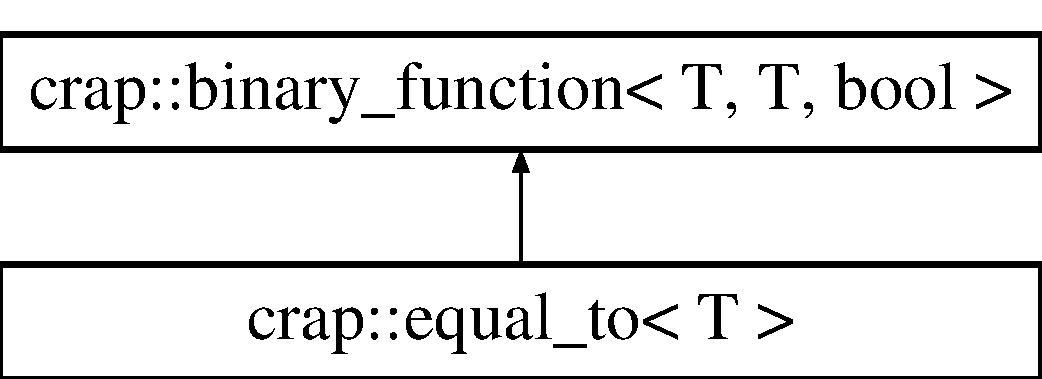
\includegraphics[height=2.000000cm]{structcrap_1_1equal__to}
\end{center}
\end{figure}
\subsection*{Public Member Functions}
\begin{DoxyCompactItemize}
\item 
bool \hyperlink{structcrap_1_1equal__to_a8b7c3c4cb07f59563639f589082dd2b6}{operator()} (const T \&x, const T \&y) const 
\end{DoxyCompactItemize}
\subsection*{Additional Inherited Members}


\subsection{Detailed Description}
\subsubsection*{template$<$class T$>$struct crap\-::equal\-\_\-to$<$ T $>$}

check if first argument is equal to second 

\subsection{Member Function Documentation}
\hypertarget{structcrap_1_1equal__to_a8b7c3c4cb07f59563639f589082dd2b6}{\index{crap\-::equal\-\_\-to@{crap\-::equal\-\_\-to}!operator()@{operator()}}
\index{operator()@{operator()}!crap::equal_to@{crap\-::equal\-\_\-to}}
\subsubsection[{operator()}]{\setlength{\rightskip}{0pt plus 5cm}template$<$class T $>$ bool {\bf crap\-::equal\-\_\-to}$<$ T $>$\-::operator() (
\begin{DoxyParamCaption}
\item[{const T \&}]{x, }
\item[{const T \&}]{y}
\end{DoxyParamCaption}
) const\hspace{0.3cm}{\ttfamily [inline]}}}\label{structcrap_1_1equal__to_a8b7c3c4cb07f59563639f589082dd2b6}


The documentation for this struct was generated from the following file\-:\begin{DoxyCompactItemize}
\item 
/mnt/windows/data/\-Programmierung/\-C\-R\-A\-P/src/crap/control/\hyperlink{compare_8h}{compare.\-h}\end{DoxyCompactItemize}

\hypertarget{classcrap_1_1functor__thread}{\section{crap\-:\-:functor\-\_\-thread$<$ T $>$ Class Template Reference}
\label{classcrap_1_1functor__thread}\index{crap\-::functor\-\_\-thread$<$ T $>$@{crap\-::functor\-\_\-thread$<$ T $>$}}
}


{\ttfamily \#include $<$functorthread.\-h$>$}

\subsection*{Public Member Functions}
\begin{DoxyCompactItemize}
\item 
\hyperlink{classcrap_1_1functor__thread_a7ab58224af9027bfd4b2764c63ce01b9}{functor\-\_\-thread} (void)
\begin{DoxyCompactList}\small\item\em default constructor \end{DoxyCompactList}\item 
\hyperlink{classcrap_1_1functor__thread_ab0da9c161a89d8ffbecf83ed0e498564}{$\sim$functor\-\_\-thread} (void)
\begin{DoxyCompactList}\small\item\em destructor \end{DoxyCompactList}\item 
\hyperlink{threading_8h_a14c0f3061b88e46a595ca858fed22b03}{T\-H\-R\-E\-A\-D\-\_\-\-H\-A\-N\-D\-L\-E} \hyperlink{classcrap_1_1functor__thread_ac8c029bb5ad6352c271bb44ba3d78ce2}{start} (void)
\begin{DoxyCompactList}\small\item\em starting thread, returning handle \end{DoxyCompactList}\item 
bool \hyperlink{classcrap_1_1functor__thread_a05dbbfe8854c00b060ff8c1be3ef22a7}{join} (void) const 
\item 
bool \hyperlink{classcrap_1_1functor__thread_a7229400ebf7b59abbab464285d2bf24b}{kill} (void)
\item 
\hyperlink{threading_8h_a14c0f3061b88e46a595ca858fed22b03}{T\-H\-R\-E\-A\-D\-\_\-\-H\-A\-N\-D\-L\-E} \hyperlink{classcrap_1_1functor__thread_aad99a90b20f331abf7152c3e04dee4b7}{thread\-\_\-id} (void)
\item 
bool \hyperlink{classcrap_1_1functor__thread_ab6ac5118e9c7b8e386b71f03d079dc11}{is\-\_\-running} (void)
\end{DoxyCompactItemize}


\subsection{Constructor \& Destructor Documentation}
\hypertarget{classcrap_1_1functor__thread_a7ab58224af9027bfd4b2764c63ce01b9}{\index{crap\-::functor\-\_\-thread@{crap\-::functor\-\_\-thread}!functor\-\_\-thread@{functor\-\_\-thread}}
\index{functor\-\_\-thread@{functor\-\_\-thread}!crap::functor_thread@{crap\-::functor\-\_\-thread}}
\subsubsection[{functor\-\_\-thread}]{\setlength{\rightskip}{0pt plus 5cm}template$<$class T $>$ {\bf crap\-::functor\-\_\-thread}$<$ T $>$\-::{\bf functor\-\_\-thread} (
\begin{DoxyParamCaption}
\item[{void}]{}
\end{DoxyParamCaption}
)}}\label{classcrap_1_1functor__thread_a7ab58224af9027bfd4b2764c63ce01b9}


default constructor 

\hypertarget{classcrap_1_1functor__thread_ab0da9c161a89d8ffbecf83ed0e498564}{\index{crap\-::functor\-\_\-thread@{crap\-::functor\-\_\-thread}!$\sim$functor\-\_\-thread@{$\sim$functor\-\_\-thread}}
\index{$\sim$functor\-\_\-thread@{$\sim$functor\-\_\-thread}!crap::functor_thread@{crap\-::functor\-\_\-thread}}
\subsubsection[{$\sim$functor\-\_\-thread}]{\setlength{\rightskip}{0pt plus 5cm}template$<$class T $>$ {\bf crap\-::functor\-\_\-thread}$<$ T $>$\-::$\sim${\bf functor\-\_\-thread} (
\begin{DoxyParamCaption}
\item[{void}]{}
\end{DoxyParamCaption}
)}}\label{classcrap_1_1functor__thread_ab0da9c161a89d8ffbecf83ed0e498564}


destructor 



\subsection{Member Function Documentation}
\hypertarget{classcrap_1_1functor__thread_ab6ac5118e9c7b8e386b71f03d079dc11}{\index{crap\-::functor\-\_\-thread@{crap\-::functor\-\_\-thread}!is\-\_\-running@{is\-\_\-running}}
\index{is\-\_\-running@{is\-\_\-running}!crap::functor_thread@{crap\-::functor\-\_\-thread}}
\subsubsection[{is\-\_\-running}]{\setlength{\rightskip}{0pt plus 5cm}template$<$class T $>$ bool {\bf crap\-::functor\-\_\-thread}$<$ T $>$\-::is\-\_\-running (
\begin{DoxyParamCaption}
\item[{void}]{}
\end{DoxyParamCaption}
)}}\label{classcrap_1_1functor__thread_ab6ac5118e9c7b8e386b71f03d079dc11}
\hypertarget{classcrap_1_1functor__thread_a05dbbfe8854c00b060ff8c1be3ef22a7}{\index{crap\-::functor\-\_\-thread@{crap\-::functor\-\_\-thread}!join@{join}}
\index{join@{join}!crap::functor_thread@{crap\-::functor\-\_\-thread}}
\subsubsection[{join}]{\setlength{\rightskip}{0pt plus 5cm}template$<$class T $>$ bool {\bf crap\-::functor\-\_\-thread}$<$ T $>$\-::join (
\begin{DoxyParamCaption}
\item[{void}]{}
\end{DoxyParamCaption}
) const}}\label{classcrap_1_1functor__thread_a05dbbfe8854c00b060ff8c1be3ef22a7}
\hypertarget{classcrap_1_1functor__thread_a7229400ebf7b59abbab464285d2bf24b}{\index{crap\-::functor\-\_\-thread@{crap\-::functor\-\_\-thread}!kill@{kill}}
\index{kill@{kill}!crap::functor_thread@{crap\-::functor\-\_\-thread}}
\subsubsection[{kill}]{\setlength{\rightskip}{0pt plus 5cm}template$<$class T $>$ bool {\bf crap\-::functor\-\_\-thread}$<$ T $>$\-::kill (
\begin{DoxyParamCaption}
\item[{void}]{}
\end{DoxyParamCaption}
)}}\label{classcrap_1_1functor__thread_a7229400ebf7b59abbab464285d2bf24b}
\hypertarget{classcrap_1_1functor__thread_ac8c029bb5ad6352c271bb44ba3d78ce2}{\index{crap\-::functor\-\_\-thread@{crap\-::functor\-\_\-thread}!start@{start}}
\index{start@{start}!crap::functor_thread@{crap\-::functor\-\_\-thread}}
\subsubsection[{start}]{\setlength{\rightskip}{0pt plus 5cm}template$<$class T $>$ {\bf T\-H\-R\-E\-A\-D\-\_\-\-H\-A\-N\-D\-L\-E} {\bf crap\-::functor\-\_\-thread}$<$ T $>$\-::start (
\begin{DoxyParamCaption}
\item[{void}]{}
\end{DoxyParamCaption}
)}}\label{classcrap_1_1functor__thread_ac8c029bb5ad6352c271bb44ba3d78ce2}


starting thread, returning handle 

\hypertarget{classcrap_1_1functor__thread_aad99a90b20f331abf7152c3e04dee4b7}{\index{crap\-::functor\-\_\-thread@{crap\-::functor\-\_\-thread}!thread\-\_\-id@{thread\-\_\-id}}
\index{thread\-\_\-id@{thread\-\_\-id}!crap::functor_thread@{crap\-::functor\-\_\-thread}}
\subsubsection[{thread\-\_\-id}]{\setlength{\rightskip}{0pt plus 5cm}template$<$class T $>$ {\bf T\-H\-R\-E\-A\-D\-\_\-\-H\-A\-N\-D\-L\-E} {\bf crap\-::functor\-\_\-thread}$<$ T $>$\-::thread\-\_\-id (
\begin{DoxyParamCaption}
\item[{void}]{}
\end{DoxyParamCaption}
)}}\label{classcrap_1_1functor__thread_aad99a90b20f331abf7152c3e04dee4b7}


The documentation for this class was generated from the following file\-:\begin{DoxyCompactItemize}
\item 
/mnt/windows/data/\-Programmierung/\-C\-R\-A\-P/src/crap/threading/\hyperlink{functorthread_8h}{functorthread.\-h}\end{DoxyCompactItemize}

\hypertarget{structcrap_1_1greater}{\section{crap\-:\-:greater$<$ T $>$ Struct Template Reference}
\label{structcrap_1_1greater}\index{crap\-::greater$<$ T $>$@{crap\-::greater$<$ T $>$}}
}


check if first argument is greater then second  




{\ttfamily \#include $<$compare.\-h$>$}

Inheritance diagram for crap\-:\-:greater$<$ T $>$\-:\begin{figure}[H]
\begin{center}
\leavevmode
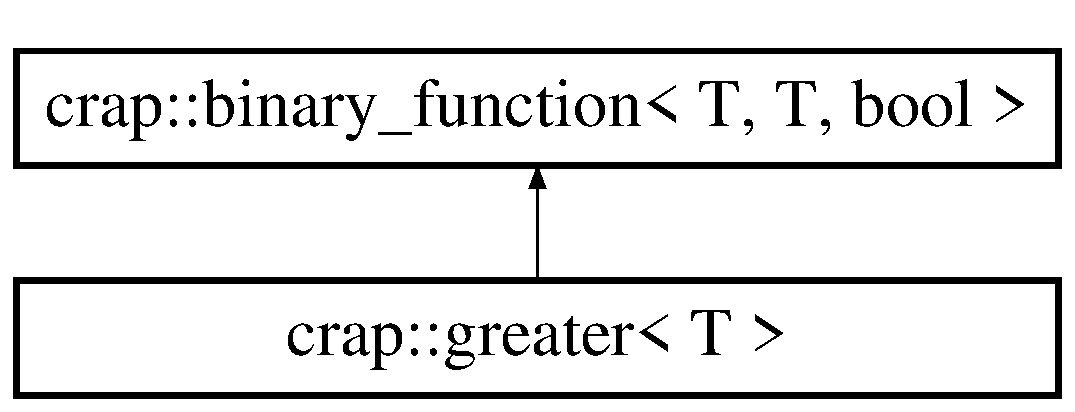
\includegraphics[height=2.000000cm]{structcrap_1_1greater}
\end{center}
\end{figure}
\subsection*{Public Member Functions}
\begin{DoxyCompactItemize}
\item 
bool \hyperlink{structcrap_1_1greater_aa32ef17b3cb751cedc71aeae6c067903}{operator()} (const T \&x, const T \&y) const 
\end{DoxyCompactItemize}
\subsection*{Additional Inherited Members}


\subsection{Detailed Description}
\subsubsection*{template$<$class T$>$struct crap\-::greater$<$ T $>$}

check if first argument is greater then second 

\subsection{Member Function Documentation}
\hypertarget{structcrap_1_1greater_aa32ef17b3cb751cedc71aeae6c067903}{\index{crap\-::greater@{crap\-::greater}!operator()@{operator()}}
\index{operator()@{operator()}!crap::greater@{crap\-::greater}}
\subsubsection[{operator()}]{\setlength{\rightskip}{0pt plus 5cm}template$<$class T $>$ bool {\bf crap\-::greater}$<$ T $>$\-::operator() (
\begin{DoxyParamCaption}
\item[{const T \&}]{x, }
\item[{const T \&}]{y}
\end{DoxyParamCaption}
) const\hspace{0.3cm}{\ttfamily [inline]}}}\label{structcrap_1_1greater_aa32ef17b3cb751cedc71aeae6c067903}


The documentation for this struct was generated from the following file\-:\begin{DoxyCompactItemize}
\item 
/mnt/windows/data/\-Programmierung/\-C\-R\-A\-P/src/crap/control/\hyperlink{compare_8h}{compare.\-h}\end{DoxyCompactItemize}

\hypertarget{structcrap_1_1greater__equal}{\section{crap\-:\-:greater\-\_\-equal$<$ T $>$ Struct Template Reference}
\label{structcrap_1_1greater__equal}\index{crap\-::greater\-\_\-equal$<$ T $>$@{crap\-::greater\-\_\-equal$<$ T $>$}}
}


check if first argument is greater equal then second  




{\ttfamily \#include $<$compare.\-h$>$}

Inheritance diagram for crap\-:\-:greater\-\_\-equal$<$ T $>$\-:\begin{figure}[H]
\begin{center}
\leavevmode
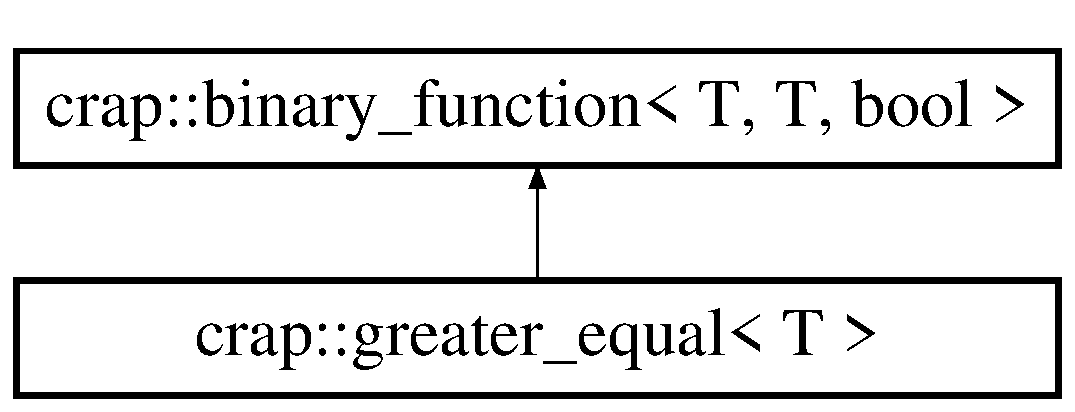
\includegraphics[height=2.000000cm]{structcrap_1_1greater__equal}
\end{center}
\end{figure}
\subsection*{Public Member Functions}
\begin{DoxyCompactItemize}
\item 
bool \hyperlink{structcrap_1_1greater__equal_a607e6ea7bc9c9f41c6b63e7eae803a41}{operator()} (const T \&x, const T \&y) const 
\end{DoxyCompactItemize}
\subsection*{Additional Inherited Members}


\subsection{Detailed Description}
\subsubsection*{template$<$class T$>$struct crap\-::greater\-\_\-equal$<$ T $>$}

check if first argument is greater equal then second 

\subsection{Member Function Documentation}
\hypertarget{structcrap_1_1greater__equal_a607e6ea7bc9c9f41c6b63e7eae803a41}{\index{crap\-::greater\-\_\-equal@{crap\-::greater\-\_\-equal}!operator()@{operator()}}
\index{operator()@{operator()}!crap::greater_equal@{crap\-::greater\-\_\-equal}}
\subsubsection[{operator()}]{\setlength{\rightskip}{0pt plus 5cm}template$<$class T $>$ bool {\bf crap\-::greater\-\_\-equal}$<$ T $>$\-::operator() (
\begin{DoxyParamCaption}
\item[{const T \&}]{x, }
\item[{const T \&}]{y}
\end{DoxyParamCaption}
) const\hspace{0.3cm}{\ttfamily [inline]}}}\label{structcrap_1_1greater__equal_a607e6ea7bc9c9f41c6b63e7eae803a41}


The documentation for this struct was generated from the following file\-:\begin{DoxyCompactItemize}
\item 
/mnt/windows/data/\-Programmierung/\-C\-R\-A\-P/src/crap/control/\hyperlink{compare_8h}{compare.\-h}\end{DoxyCompactItemize}

\hypertarget{structcrap_1_1has__vtable}{\section{crap\-:\-:has\-\_\-vtable$<$ T $>$ Struct Template Reference}
\label{structcrap_1_1has__vtable}\index{crap\-::has\-\_\-vtable$<$ T $>$@{crap\-::has\-\_\-vtable$<$ T $>$}}
}


{\ttfamily \#include $<$checkvtable.\-h$>$}

\subsection*{Classes}
\begin{DoxyCompactItemize}
\item 
struct \hyperlink{structcrap_1_1has__vtable_1_1test__class}{test\-\_\-class}
\end{DoxyCompactItemize}
\subsection*{Static Public Attributes}
\begin{DoxyCompactItemize}
\item 
static const bool \hyperlink{structcrap_1_1has__vtable_a020726388c42488ee23dc65f8e1b4b83}{R\-E\-S\-U\-L\-T} = (sizeof(\hyperlink{structcrap_1_1has__vtable_1_1test__class}{test\-\_\-class}) == sizeof(T))
\end{DoxyCompactItemize}


\subsection{Member Data Documentation}
\hypertarget{structcrap_1_1has__vtable_a020726388c42488ee23dc65f8e1b4b83}{\index{crap\-::has\-\_\-vtable@{crap\-::has\-\_\-vtable}!R\-E\-S\-U\-L\-T@{R\-E\-S\-U\-L\-T}}
\index{R\-E\-S\-U\-L\-T@{R\-E\-S\-U\-L\-T}!crap::has_vtable@{crap\-::has\-\_\-vtable}}
\subsubsection[{R\-E\-S\-U\-L\-T}]{\setlength{\rightskip}{0pt plus 5cm}template$<$class T $>$ const bool {\bf crap\-::has\-\_\-vtable}$<$ T $>$\-::R\-E\-S\-U\-L\-T = (sizeof({\bf test\-\_\-class}) == sizeof(T))\hspace{0.3cm}{\ttfamily [static]}}}\label{structcrap_1_1has__vtable_a020726388c42488ee23dc65f8e1b4b83}


The documentation for this struct was generated from the following file\-:\begin{DoxyCompactItemize}
\item 
/mnt/windows/data/\-Programmierung/\-C\-R\-A\-P/src/crap/control/\hyperlink{checkvtable_8h}{checkvtable.\-h}\end{DoxyCompactItemize}

\hypertarget{structcrap_1_1has__vtable_3_01b8_01_4}{\section{crap\-:\-:has\-\_\-vtable$<$ b8 $>$ Struct Template Reference}
\label{structcrap_1_1has__vtable_3_01b8_01_4}\index{crap\-::has\-\_\-vtable$<$ b8 $>$@{crap\-::has\-\_\-vtable$<$ b8 $>$}}
}


{\ttfamily \#include $<$checkvtable.\-h$>$}

\subsection*{Static Public Attributes}
\begin{DoxyCompactItemize}
\item 
static const bool \hyperlink{structcrap_1_1has__vtable_3_01b8_01_4_aa41a048f75d27699858a6168ae3697d7}{R\-E\-S\-U\-L\-T} = false
\end{DoxyCompactItemize}


\subsection{Member Data Documentation}
\hypertarget{structcrap_1_1has__vtable_3_01b8_01_4_aa41a048f75d27699858a6168ae3697d7}{\index{crap\-::has\-\_\-vtable$<$ b8 $>$@{crap\-::has\-\_\-vtable$<$ b8 $>$}!R\-E\-S\-U\-L\-T@{R\-E\-S\-U\-L\-T}}
\index{R\-E\-S\-U\-L\-T@{R\-E\-S\-U\-L\-T}!crap::has_vtable< b8 >@{crap\-::has\-\_\-vtable$<$ b8 $>$}}
\subsubsection[{R\-E\-S\-U\-L\-T}]{\setlength{\rightskip}{0pt plus 5cm}const bool {\bf crap\-::has\-\_\-vtable}$<$ {\bf b8} $>$\-::R\-E\-S\-U\-L\-T = false\hspace{0.3cm}{\ttfamily [static]}}}\label{structcrap_1_1has__vtable_3_01b8_01_4_aa41a048f75d27699858a6168ae3697d7}


The documentation for this struct was generated from the following file\-:\begin{DoxyCompactItemize}
\item 
/mnt/windows/data/\-Programmierung/\-C\-R\-A\-P/src/crap/control/\hyperlink{checkvtable_8h}{checkvtable.\-h}\end{DoxyCompactItemize}

\hypertarget{structcrap_1_1has__vtable_3_01c8_01_4}{\section{crap\-:\-:has\-\_\-vtable$<$ c8 $>$ Struct Template Reference}
\label{structcrap_1_1has__vtable_3_01c8_01_4}\index{crap\-::has\-\_\-vtable$<$ c8 $>$@{crap\-::has\-\_\-vtable$<$ c8 $>$}}
}


{\ttfamily \#include $<$checkvtable.\-h$>$}

\subsection*{Static Public Attributes}
\begin{DoxyCompactItemize}
\item 
static const bool \hyperlink{structcrap_1_1has__vtable_3_01c8_01_4_acb52a40025dffeab43ce51ab6857b647}{R\-E\-S\-U\-L\-T} = false
\end{DoxyCompactItemize}


\subsection{Member Data Documentation}
\hypertarget{structcrap_1_1has__vtable_3_01c8_01_4_acb52a40025dffeab43ce51ab6857b647}{\index{crap\-::has\-\_\-vtable$<$ c8 $>$@{crap\-::has\-\_\-vtable$<$ c8 $>$}!R\-E\-S\-U\-L\-T@{R\-E\-S\-U\-L\-T}}
\index{R\-E\-S\-U\-L\-T@{R\-E\-S\-U\-L\-T}!crap::has_vtable< c8 >@{crap\-::has\-\_\-vtable$<$ c8 $>$}}
\subsubsection[{R\-E\-S\-U\-L\-T}]{\setlength{\rightskip}{0pt plus 5cm}const bool {\bf crap\-::has\-\_\-vtable}$<$ {\bf c8} $>$\-::R\-E\-S\-U\-L\-T = false\hspace{0.3cm}{\ttfamily [static]}}}\label{structcrap_1_1has__vtable_3_01c8_01_4_acb52a40025dffeab43ce51ab6857b647}


The documentation for this struct was generated from the following file\-:\begin{DoxyCompactItemize}
\item 
/mnt/windows/data/\-Programmierung/\-C\-R\-A\-P/src/crap/control/\hyperlink{checkvtable_8h}{checkvtable.\-h}\end{DoxyCompactItemize}

\hypertarget{structcrap_1_1has__vtable_3_01f32_01_4}{\section{crap\-:\-:has\-\_\-vtable$<$ f32 $>$ Struct Template Reference}
\label{structcrap_1_1has__vtable_3_01f32_01_4}\index{crap\-::has\-\_\-vtable$<$ f32 $>$@{crap\-::has\-\_\-vtable$<$ f32 $>$}}
}


{\ttfamily \#include $<$checkvtable.\-h$>$}

\subsection*{Static Public Attributes}
\begin{DoxyCompactItemize}
\item 
static const bool \hyperlink{structcrap_1_1has__vtable_3_01f32_01_4_a2bef57fccaf90e998c4c6eefae20c455}{R\-E\-S\-U\-L\-T} = false
\end{DoxyCompactItemize}


\subsection{Member Data Documentation}
\hypertarget{structcrap_1_1has__vtable_3_01f32_01_4_a2bef57fccaf90e998c4c6eefae20c455}{\index{crap\-::has\-\_\-vtable$<$ f32 $>$@{crap\-::has\-\_\-vtable$<$ f32 $>$}!R\-E\-S\-U\-L\-T@{R\-E\-S\-U\-L\-T}}
\index{R\-E\-S\-U\-L\-T@{R\-E\-S\-U\-L\-T}!crap::has_vtable< f32 >@{crap\-::has\-\_\-vtable$<$ f32 $>$}}
\subsubsection[{R\-E\-S\-U\-L\-T}]{\setlength{\rightskip}{0pt plus 5cm}const bool {\bf crap\-::has\-\_\-vtable}$<$ {\bf f32} $>$\-::R\-E\-S\-U\-L\-T = false\hspace{0.3cm}{\ttfamily [static]}}}\label{structcrap_1_1has__vtable_3_01f32_01_4_a2bef57fccaf90e998c4c6eefae20c455}


The documentation for this struct was generated from the following file\-:\begin{DoxyCompactItemize}
\item 
/mnt/windows/data/\-Programmierung/\-C\-R\-A\-P/src/crap/control/\hyperlink{checkvtable_8h}{checkvtable.\-h}\end{DoxyCompactItemize}

\hypertarget{structcrap_1_1has__vtable_3_01f64_01_4}{\section{crap\-:\-:has\-\_\-vtable$<$ f64 $>$ Struct Template Reference}
\label{structcrap_1_1has__vtable_3_01f64_01_4}\index{crap\-::has\-\_\-vtable$<$ f64 $>$@{crap\-::has\-\_\-vtable$<$ f64 $>$}}
}


{\ttfamily \#include $<$checkvtable.\-h$>$}

\subsection*{Static Public Attributes}
\begin{DoxyCompactItemize}
\item 
static const bool \hyperlink{structcrap_1_1has__vtable_3_01f64_01_4_abf7cca7fd109cbadc33b642483ecaa69}{R\-E\-S\-U\-L\-T} = false
\end{DoxyCompactItemize}


\subsection{Member Data Documentation}
\hypertarget{structcrap_1_1has__vtable_3_01f64_01_4_abf7cca7fd109cbadc33b642483ecaa69}{\index{crap\-::has\-\_\-vtable$<$ f64 $>$@{crap\-::has\-\_\-vtable$<$ f64 $>$}!R\-E\-S\-U\-L\-T@{R\-E\-S\-U\-L\-T}}
\index{R\-E\-S\-U\-L\-T@{R\-E\-S\-U\-L\-T}!crap::has_vtable< f64 >@{crap\-::has\-\_\-vtable$<$ f64 $>$}}
\subsubsection[{R\-E\-S\-U\-L\-T}]{\setlength{\rightskip}{0pt plus 5cm}const bool {\bf crap\-::has\-\_\-vtable}$<$ {\bf f64} $>$\-::R\-E\-S\-U\-L\-T = false\hspace{0.3cm}{\ttfamily [static]}}}\label{structcrap_1_1has__vtable_3_01f64_01_4_abf7cca7fd109cbadc33b642483ecaa69}


The documentation for this struct was generated from the following file\-:\begin{DoxyCompactItemize}
\item 
/mnt/windows/data/\-Programmierung/\-C\-R\-A\-P/src/crap/control/\hyperlink{checkvtable_8h}{checkvtable.\-h}\end{DoxyCompactItemize}

\hypertarget{structcrap_1_1has__vtable_3_01i16_01_4}{\section{crap\-:\-:has\-\_\-vtable$<$ i16 $>$ Struct Template Reference}
\label{structcrap_1_1has__vtable_3_01i16_01_4}\index{crap\-::has\-\_\-vtable$<$ i16 $>$@{crap\-::has\-\_\-vtable$<$ i16 $>$}}
}


{\ttfamily \#include $<$checkvtable.\-h$>$}

\subsection*{Static Public Attributes}
\begin{DoxyCompactItemize}
\item 
static const bool \hyperlink{structcrap_1_1has__vtable_3_01i16_01_4_a660892f8feaf9d934ab8d3d202f65b8a}{R\-E\-S\-U\-L\-T} = false
\end{DoxyCompactItemize}


\subsection{Member Data Documentation}
\hypertarget{structcrap_1_1has__vtable_3_01i16_01_4_a660892f8feaf9d934ab8d3d202f65b8a}{\index{crap\-::has\-\_\-vtable$<$ i16 $>$@{crap\-::has\-\_\-vtable$<$ i16 $>$}!R\-E\-S\-U\-L\-T@{R\-E\-S\-U\-L\-T}}
\index{R\-E\-S\-U\-L\-T@{R\-E\-S\-U\-L\-T}!crap::has_vtable< i16 >@{crap\-::has\-\_\-vtable$<$ i16 $>$}}
\subsubsection[{R\-E\-S\-U\-L\-T}]{\setlength{\rightskip}{0pt plus 5cm}const bool {\bf crap\-::has\-\_\-vtable}$<$ {\bf i16} $>$\-::R\-E\-S\-U\-L\-T = false\hspace{0.3cm}{\ttfamily [static]}}}\label{structcrap_1_1has__vtable_3_01i16_01_4_a660892f8feaf9d934ab8d3d202f65b8a}


The documentation for this struct was generated from the following file\-:\begin{DoxyCompactItemize}
\item 
/mnt/windows/data/\-Programmierung/\-C\-R\-A\-P/src/crap/control/\hyperlink{checkvtable_8h}{checkvtable.\-h}\end{DoxyCompactItemize}

\hypertarget{structcrap_1_1has__vtable_3_01i32_01_4}{\section{crap\-:\-:has\-\_\-vtable$<$ i32 $>$ Struct Template Reference}
\label{structcrap_1_1has__vtable_3_01i32_01_4}\index{crap\-::has\-\_\-vtable$<$ i32 $>$@{crap\-::has\-\_\-vtable$<$ i32 $>$}}
}


{\ttfamily \#include $<$checkvtable.\-h$>$}

\subsection*{Static Public Attributes}
\begin{DoxyCompactItemize}
\item 
static const bool \hyperlink{structcrap_1_1has__vtable_3_01i32_01_4_a200a3f8dcd48d76ca33f889d57a06931}{R\-E\-S\-U\-L\-T} = false
\end{DoxyCompactItemize}


\subsection{Member Data Documentation}
\hypertarget{structcrap_1_1has__vtable_3_01i32_01_4_a200a3f8dcd48d76ca33f889d57a06931}{\index{crap\-::has\-\_\-vtable$<$ i32 $>$@{crap\-::has\-\_\-vtable$<$ i32 $>$}!R\-E\-S\-U\-L\-T@{R\-E\-S\-U\-L\-T}}
\index{R\-E\-S\-U\-L\-T@{R\-E\-S\-U\-L\-T}!crap::has_vtable< i32 >@{crap\-::has\-\_\-vtable$<$ i32 $>$}}
\subsubsection[{R\-E\-S\-U\-L\-T}]{\setlength{\rightskip}{0pt plus 5cm}const bool {\bf crap\-::has\-\_\-vtable}$<$ {\bf i32} $>$\-::R\-E\-S\-U\-L\-T = false\hspace{0.3cm}{\ttfamily [static]}}}\label{structcrap_1_1has__vtable_3_01i32_01_4_a200a3f8dcd48d76ca33f889d57a06931}


The documentation for this struct was generated from the following file\-:\begin{DoxyCompactItemize}
\item 
/mnt/windows/data/\-Programmierung/\-C\-R\-A\-P/src/crap/control/\hyperlink{checkvtable_8h}{checkvtable.\-h}\end{DoxyCompactItemize}

\hypertarget{structcrap_1_1has__vtable_3_01i64_01_4}{\section{crap\-:\-:has\-\_\-vtable$<$ i64 $>$ Struct Template Reference}
\label{structcrap_1_1has__vtable_3_01i64_01_4}\index{crap\-::has\-\_\-vtable$<$ i64 $>$@{crap\-::has\-\_\-vtable$<$ i64 $>$}}
}


{\ttfamily \#include $<$checkvtable.\-h$>$}

\subsection*{Static Public Attributes}
\begin{DoxyCompactItemize}
\item 
static const bool \hyperlink{structcrap_1_1has__vtable_3_01i64_01_4_afd19afa10a496b172943d1324fcdf08b}{R\-E\-S\-U\-L\-T} = false
\end{DoxyCompactItemize}


\subsection{Member Data Documentation}
\hypertarget{structcrap_1_1has__vtable_3_01i64_01_4_afd19afa10a496b172943d1324fcdf08b}{\index{crap\-::has\-\_\-vtable$<$ i64 $>$@{crap\-::has\-\_\-vtable$<$ i64 $>$}!R\-E\-S\-U\-L\-T@{R\-E\-S\-U\-L\-T}}
\index{R\-E\-S\-U\-L\-T@{R\-E\-S\-U\-L\-T}!crap::has_vtable< i64 >@{crap\-::has\-\_\-vtable$<$ i64 $>$}}
\subsubsection[{R\-E\-S\-U\-L\-T}]{\setlength{\rightskip}{0pt plus 5cm}const bool {\bf crap\-::has\-\_\-vtable}$<$ {\bf i64} $>$\-::R\-E\-S\-U\-L\-T = false\hspace{0.3cm}{\ttfamily [static]}}}\label{structcrap_1_1has__vtable_3_01i64_01_4_afd19afa10a496b172943d1324fcdf08b}


The documentation for this struct was generated from the following file\-:\begin{DoxyCompactItemize}
\item 
/mnt/windows/data/\-Programmierung/\-C\-R\-A\-P/src/crap/control/\hyperlink{checkvtable_8h}{checkvtable.\-h}\end{DoxyCompactItemize}

\hypertarget{structcrap_1_1has__vtable_3_01i8_01_4}{\section{crap\-:\-:has\-\_\-vtable$<$ i8 $>$ Struct Template Reference}
\label{structcrap_1_1has__vtable_3_01i8_01_4}\index{crap\-::has\-\_\-vtable$<$ i8 $>$@{crap\-::has\-\_\-vtable$<$ i8 $>$}}
}


{\ttfamily \#include $<$checkvtable.\-h$>$}

\subsection*{Static Public Attributes}
\begin{DoxyCompactItemize}
\item 
static const bool \hyperlink{structcrap_1_1has__vtable_3_01i8_01_4_a9e5893169f327a34e1cb787663eb7280}{R\-E\-S\-U\-L\-T} = false
\end{DoxyCompactItemize}


\subsection{Member Data Documentation}
\hypertarget{structcrap_1_1has__vtable_3_01i8_01_4_a9e5893169f327a34e1cb787663eb7280}{\index{crap\-::has\-\_\-vtable$<$ i8 $>$@{crap\-::has\-\_\-vtable$<$ i8 $>$}!R\-E\-S\-U\-L\-T@{R\-E\-S\-U\-L\-T}}
\index{R\-E\-S\-U\-L\-T@{R\-E\-S\-U\-L\-T}!crap::has_vtable< i8 >@{crap\-::has\-\_\-vtable$<$ i8 $>$}}
\subsubsection[{R\-E\-S\-U\-L\-T}]{\setlength{\rightskip}{0pt plus 5cm}const bool {\bf crap\-::has\-\_\-vtable}$<$ {\bf i8} $>$\-::R\-E\-S\-U\-L\-T = false\hspace{0.3cm}{\ttfamily [static]}}}\label{structcrap_1_1has__vtable_3_01i8_01_4_a9e5893169f327a34e1cb787663eb7280}


The documentation for this struct was generated from the following file\-:\begin{DoxyCompactItemize}
\item 
/mnt/windows/data/\-Programmierung/\-C\-R\-A\-P/src/crap/control/\hyperlink{checkvtable_8h}{checkvtable.\-h}\end{DoxyCompactItemize}

\hypertarget{structcrap_1_1has__vtable_3_01u16_01_4}{\section{crap\-:\-:has\-\_\-vtable$<$ u16 $>$ Struct Template Reference}
\label{structcrap_1_1has__vtable_3_01u16_01_4}\index{crap\-::has\-\_\-vtable$<$ u16 $>$@{crap\-::has\-\_\-vtable$<$ u16 $>$}}
}


{\ttfamily \#include $<$checkvtable.\-h$>$}

\subsection*{Static Public Attributes}
\begin{DoxyCompactItemize}
\item 
static const bool \hyperlink{structcrap_1_1has__vtable_3_01u16_01_4_a09cffb95ad9b11addf5e377c6525d455}{R\-E\-S\-U\-L\-T} = false
\end{DoxyCompactItemize}


\subsection{Member Data Documentation}
\hypertarget{structcrap_1_1has__vtable_3_01u16_01_4_a09cffb95ad9b11addf5e377c6525d455}{\index{crap\-::has\-\_\-vtable$<$ u16 $>$@{crap\-::has\-\_\-vtable$<$ u16 $>$}!R\-E\-S\-U\-L\-T@{R\-E\-S\-U\-L\-T}}
\index{R\-E\-S\-U\-L\-T@{R\-E\-S\-U\-L\-T}!crap::has_vtable< u16 >@{crap\-::has\-\_\-vtable$<$ u16 $>$}}
\subsubsection[{R\-E\-S\-U\-L\-T}]{\setlength{\rightskip}{0pt plus 5cm}const bool {\bf crap\-::has\-\_\-vtable}$<$ {\bf u16} $>$\-::R\-E\-S\-U\-L\-T = false\hspace{0.3cm}{\ttfamily [static]}}}\label{structcrap_1_1has__vtable_3_01u16_01_4_a09cffb95ad9b11addf5e377c6525d455}


The documentation for this struct was generated from the following file\-:\begin{DoxyCompactItemize}
\item 
/mnt/windows/data/\-Programmierung/\-C\-R\-A\-P/src/crap/control/\hyperlink{checkvtable_8h}{checkvtable.\-h}\end{DoxyCompactItemize}

\hypertarget{structcrap_1_1has__vtable_3_01u32_01_4}{\section{crap\-:\-:has\-\_\-vtable$<$ u32 $>$ Struct Template Reference}
\label{structcrap_1_1has__vtable_3_01u32_01_4}\index{crap\-::has\-\_\-vtable$<$ u32 $>$@{crap\-::has\-\_\-vtable$<$ u32 $>$}}
}


{\ttfamily \#include $<$checkvtable.\-h$>$}

\subsection*{Static Public Attributes}
\begin{DoxyCompactItemize}
\item 
static const bool \hyperlink{structcrap_1_1has__vtable_3_01u32_01_4_ae6c7fc8ec5ff2421ff10eb15297e835f}{R\-E\-S\-U\-L\-T} = false
\end{DoxyCompactItemize}


\subsection{Member Data Documentation}
\hypertarget{structcrap_1_1has__vtable_3_01u32_01_4_ae6c7fc8ec5ff2421ff10eb15297e835f}{\index{crap\-::has\-\_\-vtable$<$ u32 $>$@{crap\-::has\-\_\-vtable$<$ u32 $>$}!R\-E\-S\-U\-L\-T@{R\-E\-S\-U\-L\-T}}
\index{R\-E\-S\-U\-L\-T@{R\-E\-S\-U\-L\-T}!crap::has_vtable< u32 >@{crap\-::has\-\_\-vtable$<$ u32 $>$}}
\subsubsection[{R\-E\-S\-U\-L\-T}]{\setlength{\rightskip}{0pt plus 5cm}const bool {\bf crap\-::has\-\_\-vtable}$<$ {\bf u32} $>$\-::R\-E\-S\-U\-L\-T = false\hspace{0.3cm}{\ttfamily [static]}}}\label{structcrap_1_1has__vtable_3_01u32_01_4_ae6c7fc8ec5ff2421ff10eb15297e835f}


The documentation for this struct was generated from the following file\-:\begin{DoxyCompactItemize}
\item 
/mnt/windows/data/\-Programmierung/\-C\-R\-A\-P/src/crap/control/\hyperlink{checkvtable_8h}{checkvtable.\-h}\end{DoxyCompactItemize}

\hypertarget{structcrap_1_1has__vtable_3_01u64_01_4}{\section{crap\-:\-:has\-\_\-vtable$<$ u64 $>$ Struct Template Reference}
\label{structcrap_1_1has__vtable_3_01u64_01_4}\index{crap\-::has\-\_\-vtable$<$ u64 $>$@{crap\-::has\-\_\-vtable$<$ u64 $>$}}
}


{\ttfamily \#include $<$checkvtable.\-h$>$}

\subsection*{Static Public Attributes}
\begin{DoxyCompactItemize}
\item 
static const bool \hyperlink{structcrap_1_1has__vtable_3_01u64_01_4_a1e6518eb5d447cc59d70934dfa7d3af1}{R\-E\-S\-U\-L\-T} = false
\end{DoxyCompactItemize}


\subsection{Member Data Documentation}
\hypertarget{structcrap_1_1has__vtable_3_01u64_01_4_a1e6518eb5d447cc59d70934dfa7d3af1}{\index{crap\-::has\-\_\-vtable$<$ u64 $>$@{crap\-::has\-\_\-vtable$<$ u64 $>$}!R\-E\-S\-U\-L\-T@{R\-E\-S\-U\-L\-T}}
\index{R\-E\-S\-U\-L\-T@{R\-E\-S\-U\-L\-T}!crap::has_vtable< u64 >@{crap\-::has\-\_\-vtable$<$ u64 $>$}}
\subsubsection[{R\-E\-S\-U\-L\-T}]{\setlength{\rightskip}{0pt plus 5cm}const bool {\bf crap\-::has\-\_\-vtable}$<$ {\bf u64} $>$\-::R\-E\-S\-U\-L\-T = false\hspace{0.3cm}{\ttfamily [static]}}}\label{structcrap_1_1has__vtable_3_01u64_01_4_a1e6518eb5d447cc59d70934dfa7d3af1}


The documentation for this struct was generated from the following file\-:\begin{DoxyCompactItemize}
\item 
/mnt/windows/data/\-Programmierung/\-C\-R\-A\-P/src/crap/control/\hyperlink{checkvtable_8h}{checkvtable.\-h}\end{DoxyCompactItemize}

\hypertarget{structcrap_1_1has__vtable_3_01u8_01_4}{\section{crap\-:\-:has\-\_\-vtable$<$ u8 $>$ Struct Template Reference}
\label{structcrap_1_1has__vtable_3_01u8_01_4}\index{crap\-::has\-\_\-vtable$<$ u8 $>$@{crap\-::has\-\_\-vtable$<$ u8 $>$}}
}


{\ttfamily \#include $<$checkvtable.\-h$>$}

\subsection*{Static Public Attributes}
\begin{DoxyCompactItemize}
\item 
static const bool \hyperlink{structcrap_1_1has__vtable_3_01u8_01_4_a5caab64ac9c3206b14ae1912940c996f}{R\-E\-S\-U\-L\-T} = false
\end{DoxyCompactItemize}


\subsection{Member Data Documentation}
\hypertarget{structcrap_1_1has__vtable_3_01u8_01_4_a5caab64ac9c3206b14ae1912940c996f}{\index{crap\-::has\-\_\-vtable$<$ u8 $>$@{crap\-::has\-\_\-vtable$<$ u8 $>$}!R\-E\-S\-U\-L\-T@{R\-E\-S\-U\-L\-T}}
\index{R\-E\-S\-U\-L\-T@{R\-E\-S\-U\-L\-T}!crap::has_vtable< u8 >@{crap\-::has\-\_\-vtable$<$ u8 $>$}}
\subsubsection[{R\-E\-S\-U\-L\-T}]{\setlength{\rightskip}{0pt plus 5cm}const bool {\bf crap\-::has\-\_\-vtable}$<$ {\bf u8} $>$\-::R\-E\-S\-U\-L\-T = false\hspace{0.3cm}{\ttfamily [static]}}}\label{structcrap_1_1has__vtable_3_01u8_01_4_a5caab64ac9c3206b14ae1912940c996f}


The documentation for this struct was generated from the following file\-:\begin{DoxyCompactItemize}
\item 
/mnt/windows/data/\-Programmierung/\-C\-R\-A\-P/src/crap/control/\hyperlink{checkvtable_8h}{checkvtable.\-h}\end{DoxyCompactItemize}

\hypertarget{structcrap_1_1less}{\section{crap\-:\-:less$<$ T $>$ Struct Template Reference}
\label{structcrap_1_1less}\index{crap\-::less$<$ T $>$@{crap\-::less$<$ T $>$}}
}


check if first argument is less then second  




{\ttfamily \#include $<$compare.\-h$>$}

Inheritance diagram for crap\-:\-:less$<$ T $>$\-:\begin{figure}[H]
\begin{center}
\leavevmode
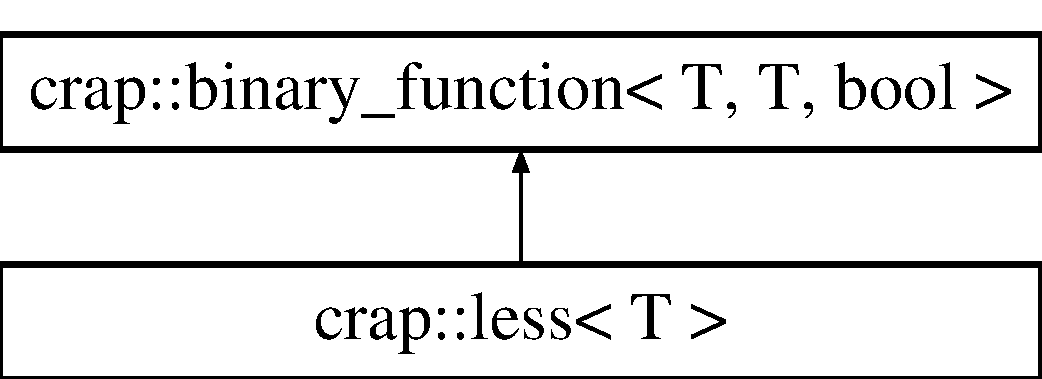
\includegraphics[height=2.000000cm]{structcrap_1_1less}
\end{center}
\end{figure}
\subsection*{Public Member Functions}
\begin{DoxyCompactItemize}
\item 
bool \hyperlink{structcrap_1_1less_af32d1b6b510d16a5ad7732cae0ceb4b8}{operator()} (const T \&x, const T \&y) const 
\end{DoxyCompactItemize}
\subsection*{Additional Inherited Members}


\subsection{Detailed Description}
\subsubsection*{template$<$class T$>$struct crap\-::less$<$ T $>$}

check if first argument is less then second 

\subsection{Member Function Documentation}
\hypertarget{structcrap_1_1less_af32d1b6b510d16a5ad7732cae0ceb4b8}{\index{crap\-::less@{crap\-::less}!operator()@{operator()}}
\index{operator()@{operator()}!crap::less@{crap\-::less}}
\subsubsection[{operator()}]{\setlength{\rightskip}{0pt plus 5cm}template$<$class T $>$ bool {\bf crap\-::less}$<$ T $>$\-::operator() (
\begin{DoxyParamCaption}
\item[{const T \&}]{x, }
\item[{const T \&}]{y}
\end{DoxyParamCaption}
) const\hspace{0.3cm}{\ttfamily [inline]}}}\label{structcrap_1_1less_af32d1b6b510d16a5ad7732cae0ceb4b8}


The documentation for this struct was generated from the following file\-:\begin{DoxyCompactItemize}
\item 
/mnt/windows/data/\-Programmierung/\-C\-R\-A\-P/src/crap/control/\hyperlink{compare_8h}{compare.\-h}\end{DoxyCompactItemize}

\hypertarget{structcrap_1_1less__equal}{\section{crap\-:\-:less\-\_\-equal$<$ T $>$ Struct Template Reference}
\label{structcrap_1_1less__equal}\index{crap\-::less\-\_\-equal$<$ T $>$@{crap\-::less\-\_\-equal$<$ T $>$}}
}


check if first argument is less equal then second  




{\ttfamily \#include $<$compare.\-h$>$}

Inheritance diagram for crap\-:\-:less\-\_\-equal$<$ T $>$\-:\begin{figure}[H]
\begin{center}
\leavevmode
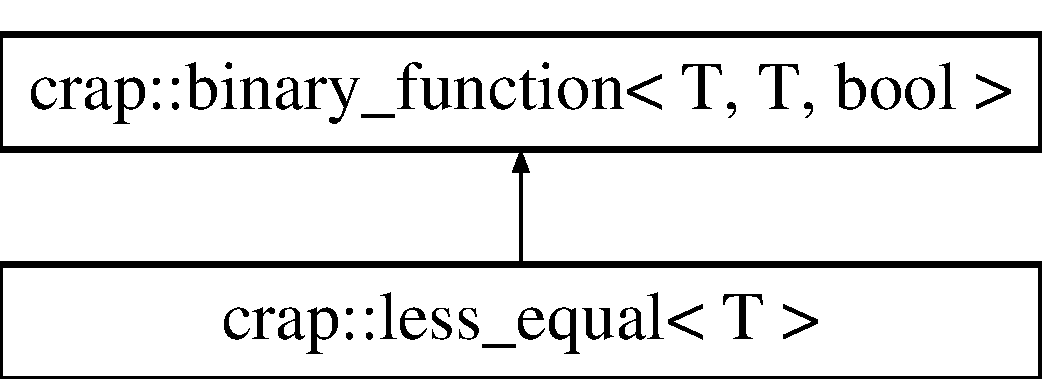
\includegraphics[height=2.000000cm]{structcrap_1_1less__equal}
\end{center}
\end{figure}
\subsection*{Public Member Functions}
\begin{DoxyCompactItemize}
\item 
bool \hyperlink{structcrap_1_1less__equal_af0f8957c39bc5b50da197e9db962a596}{operator()} (const T \&x, const T \&y) const 
\end{DoxyCompactItemize}
\subsection*{Additional Inherited Members}


\subsection{Detailed Description}
\subsubsection*{template$<$class T$>$struct crap\-::less\-\_\-equal$<$ T $>$}

check if first argument is less equal then second 

\subsection{Member Function Documentation}
\hypertarget{structcrap_1_1less__equal_af0f8957c39bc5b50da197e9db962a596}{\index{crap\-::less\-\_\-equal@{crap\-::less\-\_\-equal}!operator()@{operator()}}
\index{operator()@{operator()}!crap::less_equal@{crap\-::less\-\_\-equal}}
\subsubsection[{operator()}]{\setlength{\rightskip}{0pt plus 5cm}template$<$class T $>$ bool {\bf crap\-::less\-\_\-equal}$<$ T $>$\-::operator() (
\begin{DoxyParamCaption}
\item[{const T \&}]{x, }
\item[{const T \&}]{y}
\end{DoxyParamCaption}
) const\hspace{0.3cm}{\ttfamily [inline]}}}\label{structcrap_1_1less__equal_af0f8957c39bc5b50da197e9db962a596}


The documentation for this struct was generated from the following file\-:\begin{DoxyCompactItemize}
\item 
/mnt/windows/data/\-Programmierung/\-C\-R\-A\-P/src/crap/control/\hyperlink{compare_8h}{compare.\-h}\end{DoxyCompactItemize}

\hypertarget{structcrap_1_1less__first}{\section{crap\-:\-:less\-\_\-first$<$ T1, T2 $>$ Struct Template Reference}
\label{structcrap_1_1less__first}\index{crap\-::less\-\_\-first$<$ T1, T2 $>$@{crap\-::less\-\_\-first$<$ T1, T2 $>$}}
}


less for first (key) value  




{\ttfamily \#include $<$map.\-h$>$}

Inheritance diagram for crap\-:\-:less\-\_\-first$<$ T1, T2 $>$\-:\begin{figure}[H]
\begin{center}
\leavevmode
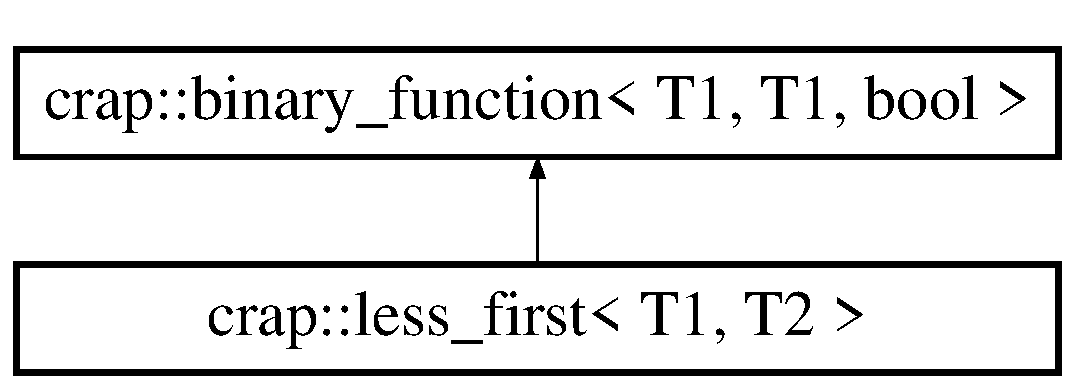
\includegraphics[height=2.000000cm]{structcrap_1_1less__first}
\end{center}
\end{figure}
\subsection*{Public Member Functions}
\begin{DoxyCompactItemize}
\item 
bool \hyperlink{structcrap_1_1less__first_ae98e8f89d1d10987f8c972fbc241759f}{operator()} (const \hyperlink{structcrap_1_1pair}{crap\-::pair}$<$ T1, T2 $>$ \&x, const \hyperlink{structcrap_1_1pair}{crap\-::pair}$<$ T1, T2 $>$ \&y) const 
\end{DoxyCompactItemize}
\subsection*{Additional Inherited Members}


\subsection{Detailed Description}
\subsubsection*{template$<$class T1, class T2$>$struct crap\-::less\-\_\-first$<$ T1, T2 $>$}

less for first (key) value 

\subsection{Member Function Documentation}
\hypertarget{structcrap_1_1less__first_ae98e8f89d1d10987f8c972fbc241759f}{\index{crap\-::less\-\_\-first@{crap\-::less\-\_\-first}!operator()@{operator()}}
\index{operator()@{operator()}!crap::less_first@{crap\-::less\-\_\-first}}
\subsubsection[{operator()}]{\setlength{\rightskip}{0pt plus 5cm}template$<$class T1 , class T2 $>$ bool {\bf crap\-::less\-\_\-first}$<$ T1, T2 $>$\-::operator() (
\begin{DoxyParamCaption}
\item[{const {\bf crap\-::pair}$<$ T1, T2 $>$ \&}]{x, }
\item[{const {\bf crap\-::pair}$<$ T1, T2 $>$ \&}]{y}
\end{DoxyParamCaption}
) const\hspace{0.3cm}{\ttfamily [inline]}}}\label{structcrap_1_1less__first_ae98e8f89d1d10987f8c972fbc241759f}


The documentation for this struct was generated from the following file\-:\begin{DoxyCompactItemize}
\item 
/mnt/windows/data/\-Programmierung/\-C\-R\-A\-P/src/crap/container/\hyperlink{map_8h}{map.\-h}\end{DoxyCompactItemize}

\hypertarget{structcrap_1_1less__second}{\section{crap\-:\-:less\-\_\-second$<$ T1, T2 $>$ Struct Template Reference}
\label{structcrap_1_1less__second}\index{crap\-::less\-\_\-second$<$ T1, T2 $>$@{crap\-::less\-\_\-second$<$ T1, T2 $>$}}
}


less for first (key) value  




{\ttfamily \#include $<$map.\-h$>$}

Inheritance diagram for crap\-:\-:less\-\_\-second$<$ T1, T2 $>$\-:\begin{figure}[H]
\begin{center}
\leavevmode
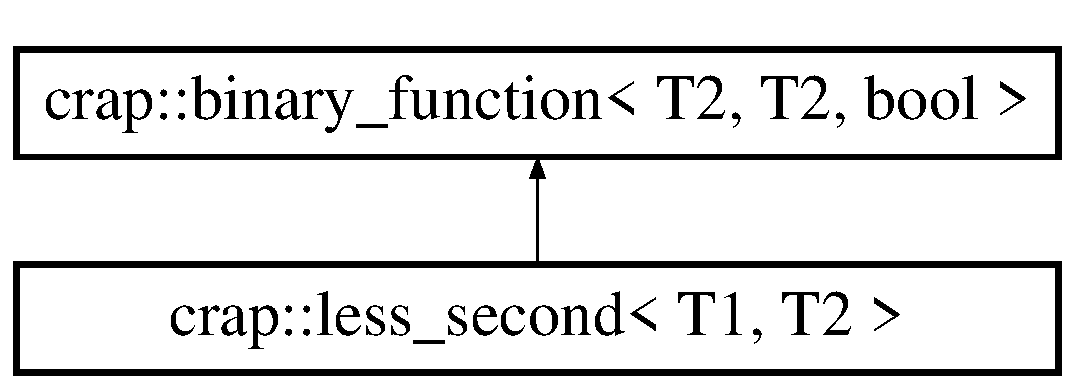
\includegraphics[height=2.000000cm]{structcrap_1_1less__second}
\end{center}
\end{figure}
\subsection*{Public Member Functions}
\begin{DoxyCompactItemize}
\item 
bool \hyperlink{structcrap_1_1less__second_a054ba6edfc2d8c6d2c5b0801700b9380}{operator()} (const \hyperlink{structcrap_1_1pair}{crap\-::pair}$<$ T1, T2 $>$ \&x, const \hyperlink{structcrap_1_1pair}{crap\-::pair}$<$ T1, T2 $>$ \&y) const 
\end{DoxyCompactItemize}
\subsection*{Additional Inherited Members}


\subsection{Detailed Description}
\subsubsection*{template$<$class T1, class T2$>$struct crap\-::less\-\_\-second$<$ T1, T2 $>$}

less for first (key) value 

\subsection{Member Function Documentation}
\hypertarget{structcrap_1_1less__second_a054ba6edfc2d8c6d2c5b0801700b9380}{\index{crap\-::less\-\_\-second@{crap\-::less\-\_\-second}!operator()@{operator()}}
\index{operator()@{operator()}!crap::less_second@{crap\-::less\-\_\-second}}
\subsubsection[{operator()}]{\setlength{\rightskip}{0pt plus 5cm}template$<$class T1 , class T2 $>$ bool {\bf crap\-::less\-\_\-second}$<$ T1, T2 $>$\-::operator() (
\begin{DoxyParamCaption}
\item[{const {\bf crap\-::pair}$<$ T1, T2 $>$ \&}]{x, }
\item[{const {\bf crap\-::pair}$<$ T1, T2 $>$ \&}]{y}
\end{DoxyParamCaption}
) const\hspace{0.3cm}{\ttfamily [inline]}}}\label{structcrap_1_1less__second_a054ba6edfc2d8c6d2c5b0801700b9380}


The documentation for this struct was generated from the following file\-:\begin{DoxyCompactItemize}
\item 
/mnt/windows/data/\-Programmierung/\-C\-R\-A\-P/src/crap/container/\hyperlink{map_8h}{map.\-h}\end{DoxyCompactItemize}

\hypertarget{structcrap_1_1limits}{\section{crap\-:\-:limits$<$ T $>$ Struct Template Reference}
\label{structcrap_1_1limits}\index{crap\-::limits$<$ T $>$@{crap\-::limits$<$ T $>$}}
}


{\ttfamily \#include $<$limits.\-h$>$}

\subsection*{Static Public Attributes}
\begin{DoxyCompactItemize}
\item 
static const T \hyperlink{structcrap_1_1limits_a0a11545145a7f4de4432d3956f1a2159}{M\-I\-N} = 0
\item 
static const T \hyperlink{structcrap_1_1limits_a757efc25bd4c43dd068be5ff95331afe}{M\-A\-X} = 0
\item 
static const bool \hyperlink{structcrap_1_1limits_a2e4a49dbaed009a912dece7de56da35e}{I\-S\-\_\-\-I\-N\-T} = true
\item 
static const bool \hyperlink{structcrap_1_1limits_a1a2b5a6b5063ca03900e9c1955db561b}{I\-S\-\_\-\-S\-I\-G\-N\-E\-D} = false
\end{DoxyCompactItemize}


\subsection{Member Data Documentation}
\hypertarget{structcrap_1_1limits_a2e4a49dbaed009a912dece7de56da35e}{\index{crap\-::limits@{crap\-::limits}!I\-S\-\_\-\-I\-N\-T@{I\-S\-\_\-\-I\-N\-T}}
\index{I\-S\-\_\-\-I\-N\-T@{I\-S\-\_\-\-I\-N\-T}!crap::limits@{crap\-::limits}}
\subsubsection[{I\-S\-\_\-\-I\-N\-T}]{\setlength{\rightskip}{0pt plus 5cm}template$<$typename T $>$ const bool {\bf crap\-::limits}$<$ T $>$\-::I\-S\-\_\-\-I\-N\-T = true\hspace{0.3cm}{\ttfamily [static]}}}\label{structcrap_1_1limits_a2e4a49dbaed009a912dece7de56da35e}
\hypertarget{structcrap_1_1limits_a1a2b5a6b5063ca03900e9c1955db561b}{\index{crap\-::limits@{crap\-::limits}!I\-S\-\_\-\-S\-I\-G\-N\-E\-D@{I\-S\-\_\-\-S\-I\-G\-N\-E\-D}}
\index{I\-S\-\_\-\-S\-I\-G\-N\-E\-D@{I\-S\-\_\-\-S\-I\-G\-N\-E\-D}!crap::limits@{crap\-::limits}}
\subsubsection[{I\-S\-\_\-\-S\-I\-G\-N\-E\-D}]{\setlength{\rightskip}{0pt plus 5cm}template$<$typename T $>$ const bool {\bf crap\-::limits}$<$ T $>$\-::I\-S\-\_\-\-S\-I\-G\-N\-E\-D = false\hspace{0.3cm}{\ttfamily [static]}}}\label{structcrap_1_1limits_a1a2b5a6b5063ca03900e9c1955db561b}
\hypertarget{structcrap_1_1limits_a757efc25bd4c43dd068be5ff95331afe}{\index{crap\-::limits@{crap\-::limits}!M\-A\-X@{M\-A\-X}}
\index{M\-A\-X@{M\-A\-X}!crap::limits@{crap\-::limits}}
\subsubsection[{M\-A\-X}]{\setlength{\rightskip}{0pt plus 5cm}template$<$typename T $>$ const T {\bf crap\-::limits}$<$ T $>$\-::M\-A\-X = 0\hspace{0.3cm}{\ttfamily [static]}}}\label{structcrap_1_1limits_a757efc25bd4c43dd068be5ff95331afe}
\hypertarget{structcrap_1_1limits_a0a11545145a7f4de4432d3956f1a2159}{\index{crap\-::limits@{crap\-::limits}!M\-I\-N@{M\-I\-N}}
\index{M\-I\-N@{M\-I\-N}!crap::limits@{crap\-::limits}}
\subsubsection[{M\-I\-N}]{\setlength{\rightskip}{0pt plus 5cm}template$<$typename T $>$ const T {\bf crap\-::limits}$<$ T $>$\-::M\-I\-N = 0\hspace{0.3cm}{\ttfamily [static]}}}\label{structcrap_1_1limits_a0a11545145a7f4de4432d3956f1a2159}


The documentation for this struct was generated from the following file\-:\begin{DoxyCompactItemize}
\item 
/mnt/windows/data/\-Programmierung/\-C\-R\-A\-P/src/crap/control/\hyperlink{limits_8h}{limits.\-h}\end{DoxyCompactItemize}

\hypertarget{structcrap_1_1limits_3_01b8_01_4}{\section{crap\-:\-:limits$<$ b8 $>$ Struct Template Reference}
\label{structcrap_1_1limits_3_01b8_01_4}\index{crap\-::limits$<$ b8 $>$@{crap\-::limits$<$ b8 $>$}}
}


{\ttfamily \#include $<$limits.\-h$>$}

\subsection*{Static Public Attributes}
\begin{DoxyCompactItemize}
\item 
static const \hyperlink{types_8h_a74eb47b4ab9e428eab7b91b3b877fa6c}{b8} \hyperlink{structcrap_1_1limits_3_01b8_01_4_ad7cee023c6e3c4ee5f1827e5becc110d}{M\-I\-N} = false
\item 
static const \hyperlink{types_8h_a74eb47b4ab9e428eab7b91b3b877fa6c}{b8} \hyperlink{structcrap_1_1limits_3_01b8_01_4_abb6122e7510a3d43e1e95a2543af6c0d}{M\-A\-X} = true
\item 
static const bool \hyperlink{structcrap_1_1limits_3_01b8_01_4_ade07f706657b5325f1d424710e1451c3}{I\-S\-\_\-\-I\-N\-T} = true
\item 
static const bool \hyperlink{structcrap_1_1limits_3_01b8_01_4_a08b3d51e6a03bb60785009fd3d68077b}{I\-S\-\_\-\-S\-I\-G\-N\-E\-D} = false
\end{DoxyCompactItemize}


\subsection{Member Data Documentation}
\hypertarget{structcrap_1_1limits_3_01b8_01_4_ade07f706657b5325f1d424710e1451c3}{\index{crap\-::limits$<$ b8 $>$@{crap\-::limits$<$ b8 $>$}!I\-S\-\_\-\-I\-N\-T@{I\-S\-\_\-\-I\-N\-T}}
\index{I\-S\-\_\-\-I\-N\-T@{I\-S\-\_\-\-I\-N\-T}!crap::limits< b8 >@{crap\-::limits$<$ b8 $>$}}
\subsubsection[{I\-S\-\_\-\-I\-N\-T}]{\setlength{\rightskip}{0pt plus 5cm}const bool {\bf crap\-::limits}$<$ {\bf b8} $>$\-::I\-S\-\_\-\-I\-N\-T = true\hspace{0.3cm}{\ttfamily [static]}}}\label{structcrap_1_1limits_3_01b8_01_4_ade07f706657b5325f1d424710e1451c3}
\hypertarget{structcrap_1_1limits_3_01b8_01_4_a08b3d51e6a03bb60785009fd3d68077b}{\index{crap\-::limits$<$ b8 $>$@{crap\-::limits$<$ b8 $>$}!I\-S\-\_\-\-S\-I\-G\-N\-E\-D@{I\-S\-\_\-\-S\-I\-G\-N\-E\-D}}
\index{I\-S\-\_\-\-S\-I\-G\-N\-E\-D@{I\-S\-\_\-\-S\-I\-G\-N\-E\-D}!crap::limits< b8 >@{crap\-::limits$<$ b8 $>$}}
\subsubsection[{I\-S\-\_\-\-S\-I\-G\-N\-E\-D}]{\setlength{\rightskip}{0pt plus 5cm}const bool {\bf crap\-::limits}$<$ {\bf b8} $>$\-::I\-S\-\_\-\-S\-I\-G\-N\-E\-D = false\hspace{0.3cm}{\ttfamily [static]}}}\label{structcrap_1_1limits_3_01b8_01_4_a08b3d51e6a03bb60785009fd3d68077b}
\hypertarget{structcrap_1_1limits_3_01b8_01_4_abb6122e7510a3d43e1e95a2543af6c0d}{\index{crap\-::limits$<$ b8 $>$@{crap\-::limits$<$ b8 $>$}!M\-A\-X@{M\-A\-X}}
\index{M\-A\-X@{M\-A\-X}!crap::limits< b8 >@{crap\-::limits$<$ b8 $>$}}
\subsubsection[{M\-A\-X}]{\setlength{\rightskip}{0pt plus 5cm}const {\bf b8} {\bf crap\-::limits}$<$ {\bf b8} $>$\-::M\-A\-X = true\hspace{0.3cm}{\ttfamily [static]}}}\label{structcrap_1_1limits_3_01b8_01_4_abb6122e7510a3d43e1e95a2543af6c0d}
\hypertarget{structcrap_1_1limits_3_01b8_01_4_ad7cee023c6e3c4ee5f1827e5becc110d}{\index{crap\-::limits$<$ b8 $>$@{crap\-::limits$<$ b8 $>$}!M\-I\-N@{M\-I\-N}}
\index{M\-I\-N@{M\-I\-N}!crap::limits< b8 >@{crap\-::limits$<$ b8 $>$}}
\subsubsection[{M\-I\-N}]{\setlength{\rightskip}{0pt plus 5cm}const {\bf b8} {\bf crap\-::limits}$<$ {\bf b8} $>$\-::M\-I\-N = false\hspace{0.3cm}{\ttfamily [static]}}}\label{structcrap_1_1limits_3_01b8_01_4_ad7cee023c6e3c4ee5f1827e5becc110d}


The documentation for this struct was generated from the following file\-:\begin{DoxyCompactItemize}
\item 
/mnt/windows/data/\-Programmierung/\-C\-R\-A\-P/src/crap/control/\hyperlink{limits_8h}{limits.\-h}\end{DoxyCompactItemize}

\hypertarget{structcrap_1_1limits_3_01c8_01_4}{\section{crap\-:\-:limits$<$ c8 $>$ Struct Template Reference}
\label{structcrap_1_1limits_3_01c8_01_4}\index{crap\-::limits$<$ c8 $>$@{crap\-::limits$<$ c8 $>$}}
}


{\ttfamily \#include $<$limits.\-h$>$}

\subsection*{Static Public Attributes}
\begin{DoxyCompactItemize}
\item 
static const \hyperlink{types_8h_aa1ba8aac9fcd831012308297336ac74b}{c8} \hyperlink{structcrap_1_1limits_3_01c8_01_4_a7cbf9e8356893e0dab215fa806292eae}{M\-I\-N} = \hyperlink{types_8h_a63e3b96e96c8d46bd4102e65f7290593}{C8\-\_\-\-M\-I\-N}
\item 
static const \hyperlink{types_8h_aa1ba8aac9fcd831012308297336ac74b}{c8} \hyperlink{structcrap_1_1limits_3_01c8_01_4_a97ae99a3786f3d5189299535e582bba8}{M\-A\-X} = \hyperlink{types_8h_ab7e171d4e3b49012ebe10417b37db364}{C8\-\_\-\-M\-A\-X}
\item 
static const bool \hyperlink{structcrap_1_1limits_3_01c8_01_4_ae087ab07a112eab4e5f69286779f86b0}{I\-S\-\_\-\-I\-N\-T} = true
\item 
static const bool \hyperlink{structcrap_1_1limits_3_01c8_01_4_ae0dc730a91615cd843450f9ae8da1c4b}{I\-S\-\_\-\-S\-I\-G\-N\-E\-D} = true
\end{DoxyCompactItemize}


\subsection{Member Data Documentation}
\hypertarget{structcrap_1_1limits_3_01c8_01_4_ae087ab07a112eab4e5f69286779f86b0}{\index{crap\-::limits$<$ c8 $>$@{crap\-::limits$<$ c8 $>$}!I\-S\-\_\-\-I\-N\-T@{I\-S\-\_\-\-I\-N\-T}}
\index{I\-S\-\_\-\-I\-N\-T@{I\-S\-\_\-\-I\-N\-T}!crap::limits< c8 >@{crap\-::limits$<$ c8 $>$}}
\subsubsection[{I\-S\-\_\-\-I\-N\-T}]{\setlength{\rightskip}{0pt plus 5cm}const bool {\bf crap\-::limits}$<$ {\bf c8} $>$\-::I\-S\-\_\-\-I\-N\-T = true\hspace{0.3cm}{\ttfamily [static]}}}\label{structcrap_1_1limits_3_01c8_01_4_ae087ab07a112eab4e5f69286779f86b0}
\hypertarget{structcrap_1_1limits_3_01c8_01_4_ae0dc730a91615cd843450f9ae8da1c4b}{\index{crap\-::limits$<$ c8 $>$@{crap\-::limits$<$ c8 $>$}!I\-S\-\_\-\-S\-I\-G\-N\-E\-D@{I\-S\-\_\-\-S\-I\-G\-N\-E\-D}}
\index{I\-S\-\_\-\-S\-I\-G\-N\-E\-D@{I\-S\-\_\-\-S\-I\-G\-N\-E\-D}!crap::limits< c8 >@{crap\-::limits$<$ c8 $>$}}
\subsubsection[{I\-S\-\_\-\-S\-I\-G\-N\-E\-D}]{\setlength{\rightskip}{0pt plus 5cm}const bool {\bf crap\-::limits}$<$ {\bf c8} $>$\-::I\-S\-\_\-\-S\-I\-G\-N\-E\-D = true\hspace{0.3cm}{\ttfamily [static]}}}\label{structcrap_1_1limits_3_01c8_01_4_ae0dc730a91615cd843450f9ae8da1c4b}
\hypertarget{structcrap_1_1limits_3_01c8_01_4_a97ae99a3786f3d5189299535e582bba8}{\index{crap\-::limits$<$ c8 $>$@{crap\-::limits$<$ c8 $>$}!M\-A\-X@{M\-A\-X}}
\index{M\-A\-X@{M\-A\-X}!crap::limits< c8 >@{crap\-::limits$<$ c8 $>$}}
\subsubsection[{M\-A\-X}]{\setlength{\rightskip}{0pt plus 5cm}const {\bf c8} {\bf crap\-::limits}$<$ {\bf c8} $>$\-::M\-A\-X = {\bf C8\-\_\-\-M\-A\-X}\hspace{0.3cm}{\ttfamily [static]}}}\label{structcrap_1_1limits_3_01c8_01_4_a97ae99a3786f3d5189299535e582bba8}
\hypertarget{structcrap_1_1limits_3_01c8_01_4_a7cbf9e8356893e0dab215fa806292eae}{\index{crap\-::limits$<$ c8 $>$@{crap\-::limits$<$ c8 $>$}!M\-I\-N@{M\-I\-N}}
\index{M\-I\-N@{M\-I\-N}!crap::limits< c8 >@{crap\-::limits$<$ c8 $>$}}
\subsubsection[{M\-I\-N}]{\setlength{\rightskip}{0pt plus 5cm}const {\bf c8} {\bf crap\-::limits}$<$ {\bf c8} $>$\-::M\-I\-N = {\bf C8\-\_\-\-M\-I\-N}\hspace{0.3cm}{\ttfamily [static]}}}\label{structcrap_1_1limits_3_01c8_01_4_a7cbf9e8356893e0dab215fa806292eae}


The documentation for this struct was generated from the following file\-:\begin{DoxyCompactItemize}
\item 
/mnt/windows/data/\-Programmierung/\-C\-R\-A\-P/src/crap/control/\hyperlink{limits_8h}{limits.\-h}\end{DoxyCompactItemize}

\hypertarget{structcrap_1_1limits_3_01f32_01_4}{\section{crap\-:\-:limits$<$ f32 $>$ Struct Template Reference}
\label{structcrap_1_1limits_3_01f32_01_4}\index{crap\-::limits$<$ f32 $>$@{crap\-::limits$<$ f32 $>$}}
}


{\ttfamily \#include $<$limits.\-h$>$}

\subsection*{Static Public Attributes}
\begin{DoxyCompactItemize}
\item 
static const \hyperlink{types_8h_a154db6eda6a99565cb060a1da4b4c930}{f32} \hyperlink{structcrap_1_1limits_3_01f32_01_4_abf95b25d77cebc19337b8e65709f837d}{M\-I\-N} = \hyperlink{types_8h_a0f9ce95191fb035fcd53ab63b9663e20}{F32\-\_\-\-M\-I\-N}
\item 
static const \hyperlink{types_8h_a154db6eda6a99565cb060a1da4b4c930}{f32} \hyperlink{structcrap_1_1limits_3_01f32_01_4_afea4f89ade14e316c4bb667d7647ca69}{M\-A\-X} = \hyperlink{types_8h_a754d8f564bd5d1fb49931b2f4c0ec00c}{F32\-\_\-\-M\-A\-X}
\item 
static const bool \hyperlink{structcrap_1_1limits_3_01f32_01_4_a131c2fe141a0c04d5140850158a0cf2d}{I\-S\-\_\-\-I\-N\-T} = false
\item 
static const bool \hyperlink{structcrap_1_1limits_3_01f32_01_4_a934f89c2f787b2d0f39a52ab4e0052b4}{I\-S\-\_\-\-S\-I\-G\-N\-E\-D} = true
\end{DoxyCompactItemize}


\subsection{Member Data Documentation}
\hypertarget{structcrap_1_1limits_3_01f32_01_4_a131c2fe141a0c04d5140850158a0cf2d}{\index{crap\-::limits$<$ f32 $>$@{crap\-::limits$<$ f32 $>$}!I\-S\-\_\-\-I\-N\-T@{I\-S\-\_\-\-I\-N\-T}}
\index{I\-S\-\_\-\-I\-N\-T@{I\-S\-\_\-\-I\-N\-T}!crap::limits< f32 >@{crap\-::limits$<$ f32 $>$}}
\subsubsection[{I\-S\-\_\-\-I\-N\-T}]{\setlength{\rightskip}{0pt plus 5cm}const bool {\bf crap\-::limits}$<$ {\bf f32} $>$\-::I\-S\-\_\-\-I\-N\-T = false\hspace{0.3cm}{\ttfamily [static]}}}\label{structcrap_1_1limits_3_01f32_01_4_a131c2fe141a0c04d5140850158a0cf2d}
\hypertarget{structcrap_1_1limits_3_01f32_01_4_a934f89c2f787b2d0f39a52ab4e0052b4}{\index{crap\-::limits$<$ f32 $>$@{crap\-::limits$<$ f32 $>$}!I\-S\-\_\-\-S\-I\-G\-N\-E\-D@{I\-S\-\_\-\-S\-I\-G\-N\-E\-D}}
\index{I\-S\-\_\-\-S\-I\-G\-N\-E\-D@{I\-S\-\_\-\-S\-I\-G\-N\-E\-D}!crap::limits< f32 >@{crap\-::limits$<$ f32 $>$}}
\subsubsection[{I\-S\-\_\-\-S\-I\-G\-N\-E\-D}]{\setlength{\rightskip}{0pt plus 5cm}const bool {\bf crap\-::limits}$<$ {\bf f32} $>$\-::I\-S\-\_\-\-S\-I\-G\-N\-E\-D = true\hspace{0.3cm}{\ttfamily [static]}}}\label{structcrap_1_1limits_3_01f32_01_4_a934f89c2f787b2d0f39a52ab4e0052b4}
\hypertarget{structcrap_1_1limits_3_01f32_01_4_afea4f89ade14e316c4bb667d7647ca69}{\index{crap\-::limits$<$ f32 $>$@{crap\-::limits$<$ f32 $>$}!M\-A\-X@{M\-A\-X}}
\index{M\-A\-X@{M\-A\-X}!crap::limits< f32 >@{crap\-::limits$<$ f32 $>$}}
\subsubsection[{M\-A\-X}]{\setlength{\rightskip}{0pt plus 5cm}const {\bf f32} {\bf crap\-::limits}$<$ {\bf f32} $>$\-::M\-A\-X = {\bf F32\-\_\-\-M\-A\-X}\hspace{0.3cm}{\ttfamily [static]}}}\label{structcrap_1_1limits_3_01f32_01_4_afea4f89ade14e316c4bb667d7647ca69}
\hypertarget{structcrap_1_1limits_3_01f32_01_4_abf95b25d77cebc19337b8e65709f837d}{\index{crap\-::limits$<$ f32 $>$@{crap\-::limits$<$ f32 $>$}!M\-I\-N@{M\-I\-N}}
\index{M\-I\-N@{M\-I\-N}!crap::limits< f32 >@{crap\-::limits$<$ f32 $>$}}
\subsubsection[{M\-I\-N}]{\setlength{\rightskip}{0pt plus 5cm}const {\bf f32} {\bf crap\-::limits}$<$ {\bf f32} $>$\-::M\-I\-N = {\bf F32\-\_\-\-M\-I\-N}\hspace{0.3cm}{\ttfamily [static]}}}\label{structcrap_1_1limits_3_01f32_01_4_abf95b25d77cebc19337b8e65709f837d}


The documentation for this struct was generated from the following files\-:\begin{DoxyCompactItemize}
\item 
/mnt/windows/data/\-Programmierung/\-C\-R\-A\-P/src/crap/control/\hyperlink{limits_8h}{limits.\-h}\item 
/mnt/windows/data/\-Programmierung/\-C\-R\-A\-P/src/crap/control/\hyperlink{limits_8cpp}{limits.\-cpp}\end{DoxyCompactItemize}

\hypertarget{structcrap_1_1limits_3_01f64_01_4}{\section{crap\-:\-:limits$<$ f64 $>$ Struct Template Reference}
\label{structcrap_1_1limits_3_01f64_01_4}\index{crap\-::limits$<$ f64 $>$@{crap\-::limits$<$ f64 $>$}}
}


{\ttfamily \#include $<$limits.\-h$>$}

\subsection*{Static Public Attributes}
\begin{DoxyCompactItemize}
\item 
static const \hyperlink{types_8h_a76c9f53497f766e57b184bc8a93ab73f}{f64} \hyperlink{structcrap_1_1limits_3_01f64_01_4_a1f7e2f5b5f8d1e47cbb95028a5dcc73a}{M\-I\-N} = \hyperlink{types_8h_a4ef26fd77745fadb40f370d63943d5eb}{F64\-\_\-\-M\-I\-N}
\item 
static const \hyperlink{types_8h_a76c9f53497f766e57b184bc8a93ab73f}{f64} \hyperlink{structcrap_1_1limits_3_01f64_01_4_aaffd447f57d01908c6549471a875b43c}{M\-A\-X} = \hyperlink{types_8h_a82daf28d8d0052302ccf95c163687ce5}{F64\-\_\-\-M\-A\-X}
\item 
static const bool \hyperlink{structcrap_1_1limits_3_01f64_01_4_a1aea3bbcfe3342c3105af4913b439c7e}{I\-S\-\_\-\-I\-N\-T} = false
\item 
static const bool \hyperlink{structcrap_1_1limits_3_01f64_01_4_a746e4464e01c3ddb2fca1ed15d66e8f5}{I\-S\-\_\-\-S\-I\-G\-N\-E\-D} = true
\end{DoxyCompactItemize}


\subsection{Member Data Documentation}
\hypertarget{structcrap_1_1limits_3_01f64_01_4_a1aea3bbcfe3342c3105af4913b439c7e}{\index{crap\-::limits$<$ f64 $>$@{crap\-::limits$<$ f64 $>$}!I\-S\-\_\-\-I\-N\-T@{I\-S\-\_\-\-I\-N\-T}}
\index{I\-S\-\_\-\-I\-N\-T@{I\-S\-\_\-\-I\-N\-T}!crap::limits< f64 >@{crap\-::limits$<$ f64 $>$}}
\subsubsection[{I\-S\-\_\-\-I\-N\-T}]{\setlength{\rightskip}{0pt plus 5cm}const bool {\bf crap\-::limits}$<$ {\bf f64} $>$\-::I\-S\-\_\-\-I\-N\-T = false\hspace{0.3cm}{\ttfamily [static]}}}\label{structcrap_1_1limits_3_01f64_01_4_a1aea3bbcfe3342c3105af4913b439c7e}
\hypertarget{structcrap_1_1limits_3_01f64_01_4_a746e4464e01c3ddb2fca1ed15d66e8f5}{\index{crap\-::limits$<$ f64 $>$@{crap\-::limits$<$ f64 $>$}!I\-S\-\_\-\-S\-I\-G\-N\-E\-D@{I\-S\-\_\-\-S\-I\-G\-N\-E\-D}}
\index{I\-S\-\_\-\-S\-I\-G\-N\-E\-D@{I\-S\-\_\-\-S\-I\-G\-N\-E\-D}!crap::limits< f64 >@{crap\-::limits$<$ f64 $>$}}
\subsubsection[{I\-S\-\_\-\-S\-I\-G\-N\-E\-D}]{\setlength{\rightskip}{0pt plus 5cm}const bool {\bf crap\-::limits}$<$ {\bf f64} $>$\-::I\-S\-\_\-\-S\-I\-G\-N\-E\-D = true\hspace{0.3cm}{\ttfamily [static]}}}\label{structcrap_1_1limits_3_01f64_01_4_a746e4464e01c3ddb2fca1ed15d66e8f5}
\hypertarget{structcrap_1_1limits_3_01f64_01_4_aaffd447f57d01908c6549471a875b43c}{\index{crap\-::limits$<$ f64 $>$@{crap\-::limits$<$ f64 $>$}!M\-A\-X@{M\-A\-X}}
\index{M\-A\-X@{M\-A\-X}!crap::limits< f64 >@{crap\-::limits$<$ f64 $>$}}
\subsubsection[{M\-A\-X}]{\setlength{\rightskip}{0pt plus 5cm}const {\bf f64} {\bf crap\-::limits}$<$ {\bf f64} $>$\-::M\-A\-X = {\bf F64\-\_\-\-M\-A\-X}\hspace{0.3cm}{\ttfamily [static]}}}\label{structcrap_1_1limits_3_01f64_01_4_aaffd447f57d01908c6549471a875b43c}
\hypertarget{structcrap_1_1limits_3_01f64_01_4_a1f7e2f5b5f8d1e47cbb95028a5dcc73a}{\index{crap\-::limits$<$ f64 $>$@{crap\-::limits$<$ f64 $>$}!M\-I\-N@{M\-I\-N}}
\index{M\-I\-N@{M\-I\-N}!crap::limits< f64 >@{crap\-::limits$<$ f64 $>$}}
\subsubsection[{M\-I\-N}]{\setlength{\rightskip}{0pt plus 5cm}const {\bf f64} {\bf crap\-::limits}$<$ {\bf f64} $>$\-::M\-I\-N = {\bf F64\-\_\-\-M\-I\-N}\hspace{0.3cm}{\ttfamily [static]}}}\label{structcrap_1_1limits_3_01f64_01_4_a1f7e2f5b5f8d1e47cbb95028a5dcc73a}


The documentation for this struct was generated from the following files\-:\begin{DoxyCompactItemize}
\item 
/mnt/windows/data/\-Programmierung/\-C\-R\-A\-P/src/crap/control/\hyperlink{limits_8h}{limits.\-h}\item 
/mnt/windows/data/\-Programmierung/\-C\-R\-A\-P/src/crap/control/\hyperlink{limits_8cpp}{limits.\-cpp}\end{DoxyCompactItemize}

\hypertarget{structcrap_1_1limits_3_01i16_01_4}{\section{crap\-:\-:limits$<$ i16 $>$ Struct Template Reference}
\label{structcrap_1_1limits_3_01i16_01_4}\index{crap\-::limits$<$ i16 $>$@{crap\-::limits$<$ i16 $>$}}
}


{\ttfamily \#include $<$limits.\-h$>$}

\subsection*{Static Public Attributes}
\begin{DoxyCompactItemize}
\item 
static const \hyperlink{types_8h_ad309dbcaeea13aa602d686964156ea0b}{i16} \hyperlink{structcrap_1_1limits_3_01i16_01_4_aa889fd67d3f189c3088083ee7fcc864d}{M\-I\-N} = \hyperlink{types_8h_a72800ba3863b6bae70ee3f22482e6db3}{I16\-\_\-\-M\-I\-N}
\item 
static const \hyperlink{types_8h_ad309dbcaeea13aa602d686964156ea0b}{i16} \hyperlink{structcrap_1_1limits_3_01i16_01_4_a13ea6e73f00832ef4ee180905c515a50}{M\-A\-X} = \hyperlink{types_8h_a31c11a64ca799bf89552369a63cecf98}{I16\-\_\-\-M\-A\-X}
\item 
static const bool \hyperlink{structcrap_1_1limits_3_01i16_01_4_a9d0b16f84b3813fe161bcd5c4758750d}{I\-S\-\_\-\-I\-N\-T} = true
\item 
static const bool \hyperlink{structcrap_1_1limits_3_01i16_01_4_acaf692f3f9189b8439fda32001539b55}{I\-S\-\_\-\-S\-I\-G\-N\-E\-D} = true
\end{DoxyCompactItemize}


\subsection{Member Data Documentation}
\hypertarget{structcrap_1_1limits_3_01i16_01_4_a9d0b16f84b3813fe161bcd5c4758750d}{\index{crap\-::limits$<$ i16 $>$@{crap\-::limits$<$ i16 $>$}!I\-S\-\_\-\-I\-N\-T@{I\-S\-\_\-\-I\-N\-T}}
\index{I\-S\-\_\-\-I\-N\-T@{I\-S\-\_\-\-I\-N\-T}!crap::limits< i16 >@{crap\-::limits$<$ i16 $>$}}
\subsubsection[{I\-S\-\_\-\-I\-N\-T}]{\setlength{\rightskip}{0pt plus 5cm}const bool {\bf crap\-::limits}$<$ {\bf i16} $>$\-::I\-S\-\_\-\-I\-N\-T = true\hspace{0.3cm}{\ttfamily [static]}}}\label{structcrap_1_1limits_3_01i16_01_4_a9d0b16f84b3813fe161bcd5c4758750d}
\hypertarget{structcrap_1_1limits_3_01i16_01_4_acaf692f3f9189b8439fda32001539b55}{\index{crap\-::limits$<$ i16 $>$@{crap\-::limits$<$ i16 $>$}!I\-S\-\_\-\-S\-I\-G\-N\-E\-D@{I\-S\-\_\-\-S\-I\-G\-N\-E\-D}}
\index{I\-S\-\_\-\-S\-I\-G\-N\-E\-D@{I\-S\-\_\-\-S\-I\-G\-N\-E\-D}!crap::limits< i16 >@{crap\-::limits$<$ i16 $>$}}
\subsubsection[{I\-S\-\_\-\-S\-I\-G\-N\-E\-D}]{\setlength{\rightskip}{0pt plus 5cm}const bool {\bf crap\-::limits}$<$ {\bf i16} $>$\-::I\-S\-\_\-\-S\-I\-G\-N\-E\-D = true\hspace{0.3cm}{\ttfamily [static]}}}\label{structcrap_1_1limits_3_01i16_01_4_acaf692f3f9189b8439fda32001539b55}
\hypertarget{structcrap_1_1limits_3_01i16_01_4_a13ea6e73f00832ef4ee180905c515a50}{\index{crap\-::limits$<$ i16 $>$@{crap\-::limits$<$ i16 $>$}!M\-A\-X@{M\-A\-X}}
\index{M\-A\-X@{M\-A\-X}!crap::limits< i16 >@{crap\-::limits$<$ i16 $>$}}
\subsubsection[{M\-A\-X}]{\setlength{\rightskip}{0pt plus 5cm}const {\bf i16} {\bf crap\-::limits}$<$ {\bf i16} $>$\-::M\-A\-X = {\bf I16\-\_\-\-M\-A\-X}\hspace{0.3cm}{\ttfamily [static]}}}\label{structcrap_1_1limits_3_01i16_01_4_a13ea6e73f00832ef4ee180905c515a50}
\hypertarget{structcrap_1_1limits_3_01i16_01_4_aa889fd67d3f189c3088083ee7fcc864d}{\index{crap\-::limits$<$ i16 $>$@{crap\-::limits$<$ i16 $>$}!M\-I\-N@{M\-I\-N}}
\index{M\-I\-N@{M\-I\-N}!crap::limits< i16 >@{crap\-::limits$<$ i16 $>$}}
\subsubsection[{M\-I\-N}]{\setlength{\rightskip}{0pt plus 5cm}const {\bf i16} {\bf crap\-::limits}$<$ {\bf i16} $>$\-::M\-I\-N = {\bf I16\-\_\-\-M\-I\-N}\hspace{0.3cm}{\ttfamily [static]}}}\label{structcrap_1_1limits_3_01i16_01_4_aa889fd67d3f189c3088083ee7fcc864d}


The documentation for this struct was generated from the following file\-:\begin{DoxyCompactItemize}
\item 
/mnt/windows/data/\-Programmierung/\-C\-R\-A\-P/src/crap/control/\hyperlink{limits_8h}{limits.\-h}\end{DoxyCompactItemize}

\hypertarget{structcrap_1_1limits_3_01i32_01_4}{\section{crap\-:\-:limits$<$ i32 $>$ Struct Template Reference}
\label{structcrap_1_1limits_3_01i32_01_4}\index{crap\-::limits$<$ i32 $>$@{crap\-::limits$<$ i32 $>$}}
}


{\ttfamily \#include $<$limits.\-h$>$}

\subsection*{Static Public Attributes}
\begin{DoxyCompactItemize}
\item 
static const \hyperlink{types_8h_a48d6cd8e4135fb2ff7e7f2dac84089ec}{i32} \hyperlink{structcrap_1_1limits_3_01i32_01_4_ab2a35d740c44e069a91e9b1a60442606}{M\-I\-N} = \hyperlink{types_8h_acf167b5064e33111b4da99625631b8af}{I32\-\_\-\-M\-I\-N}
\item 
static const \hyperlink{types_8h_a48d6cd8e4135fb2ff7e7f2dac84089ec}{i32} \hyperlink{structcrap_1_1limits_3_01i32_01_4_ab7bc98df30a82beffa2e85a1c53e5b86}{M\-A\-X} = \hyperlink{types_8h_a6e0f9d2db6ef5d899eb21081ef248851}{I32\-\_\-\-M\-A\-X}
\item 
static const bool \hyperlink{structcrap_1_1limits_3_01i32_01_4_a6cf2bcdbf1ba35d760823cdb901c94a5}{I\-S\-\_\-\-I\-N\-T} = true
\item 
static const bool \hyperlink{structcrap_1_1limits_3_01i32_01_4_a39bc0425c1c42bf8589dd42be54c4a0a}{I\-S\-\_\-\-S\-I\-G\-N\-E\-D} = true
\end{DoxyCompactItemize}


\subsection{Member Data Documentation}
\hypertarget{structcrap_1_1limits_3_01i32_01_4_a6cf2bcdbf1ba35d760823cdb901c94a5}{\index{crap\-::limits$<$ i32 $>$@{crap\-::limits$<$ i32 $>$}!I\-S\-\_\-\-I\-N\-T@{I\-S\-\_\-\-I\-N\-T}}
\index{I\-S\-\_\-\-I\-N\-T@{I\-S\-\_\-\-I\-N\-T}!crap::limits< i32 >@{crap\-::limits$<$ i32 $>$}}
\subsubsection[{I\-S\-\_\-\-I\-N\-T}]{\setlength{\rightskip}{0pt plus 5cm}const bool {\bf crap\-::limits}$<$ {\bf i32} $>$\-::I\-S\-\_\-\-I\-N\-T = true\hspace{0.3cm}{\ttfamily [static]}}}\label{structcrap_1_1limits_3_01i32_01_4_a6cf2bcdbf1ba35d760823cdb901c94a5}
\hypertarget{structcrap_1_1limits_3_01i32_01_4_a39bc0425c1c42bf8589dd42be54c4a0a}{\index{crap\-::limits$<$ i32 $>$@{crap\-::limits$<$ i32 $>$}!I\-S\-\_\-\-S\-I\-G\-N\-E\-D@{I\-S\-\_\-\-S\-I\-G\-N\-E\-D}}
\index{I\-S\-\_\-\-S\-I\-G\-N\-E\-D@{I\-S\-\_\-\-S\-I\-G\-N\-E\-D}!crap::limits< i32 >@{crap\-::limits$<$ i32 $>$}}
\subsubsection[{I\-S\-\_\-\-S\-I\-G\-N\-E\-D}]{\setlength{\rightskip}{0pt plus 5cm}const bool {\bf crap\-::limits}$<$ {\bf i32} $>$\-::I\-S\-\_\-\-S\-I\-G\-N\-E\-D = true\hspace{0.3cm}{\ttfamily [static]}}}\label{structcrap_1_1limits_3_01i32_01_4_a39bc0425c1c42bf8589dd42be54c4a0a}
\hypertarget{structcrap_1_1limits_3_01i32_01_4_ab7bc98df30a82beffa2e85a1c53e5b86}{\index{crap\-::limits$<$ i32 $>$@{crap\-::limits$<$ i32 $>$}!M\-A\-X@{M\-A\-X}}
\index{M\-A\-X@{M\-A\-X}!crap::limits< i32 >@{crap\-::limits$<$ i32 $>$}}
\subsubsection[{M\-A\-X}]{\setlength{\rightskip}{0pt plus 5cm}const {\bf i32} {\bf crap\-::limits}$<$ {\bf i32} $>$\-::M\-A\-X = {\bf I32\-\_\-\-M\-A\-X}\hspace{0.3cm}{\ttfamily [static]}}}\label{structcrap_1_1limits_3_01i32_01_4_ab7bc98df30a82beffa2e85a1c53e5b86}
\hypertarget{structcrap_1_1limits_3_01i32_01_4_ab2a35d740c44e069a91e9b1a60442606}{\index{crap\-::limits$<$ i32 $>$@{crap\-::limits$<$ i32 $>$}!M\-I\-N@{M\-I\-N}}
\index{M\-I\-N@{M\-I\-N}!crap::limits< i32 >@{crap\-::limits$<$ i32 $>$}}
\subsubsection[{M\-I\-N}]{\setlength{\rightskip}{0pt plus 5cm}const {\bf i32} {\bf crap\-::limits}$<$ {\bf i32} $>$\-::M\-I\-N = {\bf I32\-\_\-\-M\-I\-N}\hspace{0.3cm}{\ttfamily [static]}}}\label{structcrap_1_1limits_3_01i32_01_4_ab2a35d740c44e069a91e9b1a60442606}


The documentation for this struct was generated from the following file\-:\begin{DoxyCompactItemize}
\item 
/mnt/windows/data/\-Programmierung/\-C\-R\-A\-P/src/crap/control/\hyperlink{limits_8h}{limits.\-h}\end{DoxyCompactItemize}

\hypertarget{structcrap_1_1limits_3_01i64_01_4}{\section{crap\-:\-:limits$<$ i64 $>$ Struct Template Reference}
\label{structcrap_1_1limits_3_01i64_01_4}\index{crap\-::limits$<$ i64 $>$@{crap\-::limits$<$ i64 $>$}}
}


{\ttfamily \#include $<$limits.\-h$>$}

\subsection*{Static Public Attributes}
\begin{DoxyCompactItemize}
\item 
static const \hyperlink{types_8h_a85cb35fbe5bf2961d7ad5f26814a91a2}{i64} \hyperlink{structcrap_1_1limits_3_01i64_01_4_a50f4434a55e01e7dae98941d5595a6b3}{M\-I\-N} = \hyperlink{types_8h_a0427de163db0e1a357eee973c48bdfb5}{I64\-\_\-\-M\-I\-N}
\item 
static const \hyperlink{types_8h_a85cb35fbe5bf2961d7ad5f26814a91a2}{i64} \hyperlink{structcrap_1_1limits_3_01i64_01_4_af68dda1c50195c3f58e4517fc21d69f4}{M\-A\-X} = \hyperlink{types_8h_a5f660b55f835b170812ab67f556e9a5a}{I64\-\_\-\-M\-A\-X}
\item 
static const bool \hyperlink{structcrap_1_1limits_3_01i64_01_4_a1c75e13842bd5be8dc607703aa3bde20}{I\-S\-\_\-\-I\-N\-T} = true
\item 
static const bool \hyperlink{structcrap_1_1limits_3_01i64_01_4_abc50902329af13ea9041e31b99530519}{I\-S\-\_\-\-S\-I\-G\-N\-E\-D} = true
\end{DoxyCompactItemize}


\subsection{Member Data Documentation}
\hypertarget{structcrap_1_1limits_3_01i64_01_4_a1c75e13842bd5be8dc607703aa3bde20}{\index{crap\-::limits$<$ i64 $>$@{crap\-::limits$<$ i64 $>$}!I\-S\-\_\-\-I\-N\-T@{I\-S\-\_\-\-I\-N\-T}}
\index{I\-S\-\_\-\-I\-N\-T@{I\-S\-\_\-\-I\-N\-T}!crap::limits< i64 >@{crap\-::limits$<$ i64 $>$}}
\subsubsection[{I\-S\-\_\-\-I\-N\-T}]{\setlength{\rightskip}{0pt plus 5cm}const bool {\bf crap\-::limits}$<$ {\bf i64} $>$\-::I\-S\-\_\-\-I\-N\-T = true\hspace{0.3cm}{\ttfamily [static]}}}\label{structcrap_1_1limits_3_01i64_01_4_a1c75e13842bd5be8dc607703aa3bde20}
\hypertarget{structcrap_1_1limits_3_01i64_01_4_abc50902329af13ea9041e31b99530519}{\index{crap\-::limits$<$ i64 $>$@{crap\-::limits$<$ i64 $>$}!I\-S\-\_\-\-S\-I\-G\-N\-E\-D@{I\-S\-\_\-\-S\-I\-G\-N\-E\-D}}
\index{I\-S\-\_\-\-S\-I\-G\-N\-E\-D@{I\-S\-\_\-\-S\-I\-G\-N\-E\-D}!crap::limits< i64 >@{crap\-::limits$<$ i64 $>$}}
\subsubsection[{I\-S\-\_\-\-S\-I\-G\-N\-E\-D}]{\setlength{\rightskip}{0pt plus 5cm}const bool {\bf crap\-::limits}$<$ {\bf i64} $>$\-::I\-S\-\_\-\-S\-I\-G\-N\-E\-D = true\hspace{0.3cm}{\ttfamily [static]}}}\label{structcrap_1_1limits_3_01i64_01_4_abc50902329af13ea9041e31b99530519}
\hypertarget{structcrap_1_1limits_3_01i64_01_4_af68dda1c50195c3f58e4517fc21d69f4}{\index{crap\-::limits$<$ i64 $>$@{crap\-::limits$<$ i64 $>$}!M\-A\-X@{M\-A\-X}}
\index{M\-A\-X@{M\-A\-X}!crap::limits< i64 >@{crap\-::limits$<$ i64 $>$}}
\subsubsection[{M\-A\-X}]{\setlength{\rightskip}{0pt plus 5cm}const {\bf i64} {\bf crap\-::limits}$<$ {\bf i64} $>$\-::M\-A\-X = {\bf I64\-\_\-\-M\-A\-X}\hspace{0.3cm}{\ttfamily [static]}}}\label{structcrap_1_1limits_3_01i64_01_4_af68dda1c50195c3f58e4517fc21d69f4}
\hypertarget{structcrap_1_1limits_3_01i64_01_4_a50f4434a55e01e7dae98941d5595a6b3}{\index{crap\-::limits$<$ i64 $>$@{crap\-::limits$<$ i64 $>$}!M\-I\-N@{M\-I\-N}}
\index{M\-I\-N@{M\-I\-N}!crap::limits< i64 >@{crap\-::limits$<$ i64 $>$}}
\subsubsection[{M\-I\-N}]{\setlength{\rightskip}{0pt plus 5cm}const {\bf i64} {\bf crap\-::limits}$<$ {\bf i64} $>$\-::M\-I\-N = {\bf I64\-\_\-\-M\-I\-N}\hspace{0.3cm}{\ttfamily [static]}}}\label{structcrap_1_1limits_3_01i64_01_4_a50f4434a55e01e7dae98941d5595a6b3}


The documentation for this struct was generated from the following file\-:\begin{DoxyCompactItemize}
\item 
/mnt/windows/data/\-Programmierung/\-C\-R\-A\-P/src/crap/control/\hyperlink{limits_8h}{limits.\-h}\end{DoxyCompactItemize}

\hypertarget{structcrap_1_1limits_3_01i8_01_4}{\section{crap\-:\-:limits$<$ i8 $>$ Struct Template Reference}
\label{structcrap_1_1limits_3_01i8_01_4}\index{crap\-::limits$<$ i8 $>$@{crap\-::limits$<$ i8 $>$}}
}


{\ttfamily \#include $<$limits.\-h$>$}

\subsection*{Static Public Attributes}
\begin{DoxyCompactItemize}
\item 
static const \hyperlink{types_8h_ae3702327b5f47e83b431e22b33da7b58}{i8} \hyperlink{structcrap_1_1limits_3_01i8_01_4_af0166184f7c1640d6c55d91aec23122c}{M\-I\-N} = \hyperlink{types_8h_a50b6c3c5a46f347eb58da649285ddaa8}{I8\-\_\-\-M\-I\-N}
\item 
static const \hyperlink{types_8h_ae3702327b5f47e83b431e22b33da7b58}{i8} \hyperlink{structcrap_1_1limits_3_01i8_01_4_a9a112176e132c99e9a942394b144358d}{M\-A\-X} = \hyperlink{types_8h_a06aab1f97b965931eb9b623f9cc4952d}{I8\-\_\-\-M\-A\-X}
\item 
static const bool \hyperlink{structcrap_1_1limits_3_01i8_01_4_a51f3d21ce69742a7573fccdefbcd850a}{I\-S\-\_\-\-I\-N\-T} = true
\item 
static const bool \hyperlink{structcrap_1_1limits_3_01i8_01_4_aaaca3b4f389d55b8d647c522f13c1c37}{I\-S\-\_\-\-S\-I\-G\-N\-E\-D} = true
\end{DoxyCompactItemize}


\subsection{Member Data Documentation}
\hypertarget{structcrap_1_1limits_3_01i8_01_4_a51f3d21ce69742a7573fccdefbcd850a}{\index{crap\-::limits$<$ i8 $>$@{crap\-::limits$<$ i8 $>$}!I\-S\-\_\-\-I\-N\-T@{I\-S\-\_\-\-I\-N\-T}}
\index{I\-S\-\_\-\-I\-N\-T@{I\-S\-\_\-\-I\-N\-T}!crap::limits< i8 >@{crap\-::limits$<$ i8 $>$}}
\subsubsection[{I\-S\-\_\-\-I\-N\-T}]{\setlength{\rightskip}{0pt plus 5cm}const bool {\bf crap\-::limits}$<$ {\bf i8} $>$\-::I\-S\-\_\-\-I\-N\-T = true\hspace{0.3cm}{\ttfamily [static]}}}\label{structcrap_1_1limits_3_01i8_01_4_a51f3d21ce69742a7573fccdefbcd850a}
\hypertarget{structcrap_1_1limits_3_01i8_01_4_aaaca3b4f389d55b8d647c522f13c1c37}{\index{crap\-::limits$<$ i8 $>$@{crap\-::limits$<$ i8 $>$}!I\-S\-\_\-\-S\-I\-G\-N\-E\-D@{I\-S\-\_\-\-S\-I\-G\-N\-E\-D}}
\index{I\-S\-\_\-\-S\-I\-G\-N\-E\-D@{I\-S\-\_\-\-S\-I\-G\-N\-E\-D}!crap::limits< i8 >@{crap\-::limits$<$ i8 $>$}}
\subsubsection[{I\-S\-\_\-\-S\-I\-G\-N\-E\-D}]{\setlength{\rightskip}{0pt plus 5cm}const bool {\bf crap\-::limits}$<$ {\bf i8} $>$\-::I\-S\-\_\-\-S\-I\-G\-N\-E\-D = true\hspace{0.3cm}{\ttfamily [static]}}}\label{structcrap_1_1limits_3_01i8_01_4_aaaca3b4f389d55b8d647c522f13c1c37}
\hypertarget{structcrap_1_1limits_3_01i8_01_4_a9a112176e132c99e9a942394b144358d}{\index{crap\-::limits$<$ i8 $>$@{crap\-::limits$<$ i8 $>$}!M\-A\-X@{M\-A\-X}}
\index{M\-A\-X@{M\-A\-X}!crap::limits< i8 >@{crap\-::limits$<$ i8 $>$}}
\subsubsection[{M\-A\-X}]{\setlength{\rightskip}{0pt plus 5cm}const {\bf i8} {\bf crap\-::limits}$<$ {\bf i8} $>$\-::M\-A\-X = {\bf I8\-\_\-\-M\-A\-X}\hspace{0.3cm}{\ttfamily [static]}}}\label{structcrap_1_1limits_3_01i8_01_4_a9a112176e132c99e9a942394b144358d}
\hypertarget{structcrap_1_1limits_3_01i8_01_4_af0166184f7c1640d6c55d91aec23122c}{\index{crap\-::limits$<$ i8 $>$@{crap\-::limits$<$ i8 $>$}!M\-I\-N@{M\-I\-N}}
\index{M\-I\-N@{M\-I\-N}!crap::limits< i8 >@{crap\-::limits$<$ i8 $>$}}
\subsubsection[{M\-I\-N}]{\setlength{\rightskip}{0pt plus 5cm}const {\bf i8} {\bf crap\-::limits}$<$ {\bf i8} $>$\-::M\-I\-N = {\bf I8\-\_\-\-M\-I\-N}\hspace{0.3cm}{\ttfamily [static]}}}\label{structcrap_1_1limits_3_01i8_01_4_af0166184f7c1640d6c55d91aec23122c}


The documentation for this struct was generated from the following file\-:\begin{DoxyCompactItemize}
\item 
/mnt/windows/data/\-Programmierung/\-C\-R\-A\-P/src/crap/control/\hyperlink{limits_8h}{limits.\-h}\end{DoxyCompactItemize}

\hypertarget{structcrap_1_1limits_3_01u16_01_4}{\section{crap\-:\-:limits$<$ u16 $>$ Struct Template Reference}
\label{structcrap_1_1limits_3_01u16_01_4}\index{crap\-::limits$<$ u16 $>$@{crap\-::limits$<$ u16 $>$}}
}


{\ttfamily \#include $<$limits.\-h$>$}

\subsection*{Static Public Attributes}
\begin{DoxyCompactItemize}
\item 
static const \hyperlink{types_8h_ace9d960e74685e2cd84b36132dbbf8aa}{u16} \hyperlink{structcrap_1_1limits_3_01u16_01_4_ac704c0d0f11c157ac4f1a4abd49c2bb8}{M\-I\-N} = \hyperlink{types_8h_a80b4ee16c02644eef90553da09dc0907}{U16\-\_\-\-M\-I\-N}
\item 
static const \hyperlink{types_8h_ace9d960e74685e2cd84b36132dbbf8aa}{u16} \hyperlink{structcrap_1_1limits_3_01u16_01_4_afe9d8a17c2f0208f423347b1744ac06d}{M\-A\-X} = \hyperlink{types_8h_ac580728e242e90fe3082dc7fe45ec6c9}{U16\-\_\-\-M\-A\-X}
\item 
static const bool \hyperlink{structcrap_1_1limits_3_01u16_01_4_aac89c7feebcee8d2995ad4f673bd2b2b}{I\-S\-\_\-\-I\-N\-T} = true
\item 
static const bool \hyperlink{structcrap_1_1limits_3_01u16_01_4_a8b3d63b1536b733d7050d518cf81ae6a}{I\-S\-\_\-\-S\-I\-G\-N\-E\-D} = false
\end{DoxyCompactItemize}


\subsection{Member Data Documentation}
\hypertarget{structcrap_1_1limits_3_01u16_01_4_aac89c7feebcee8d2995ad4f673bd2b2b}{\index{crap\-::limits$<$ u16 $>$@{crap\-::limits$<$ u16 $>$}!I\-S\-\_\-\-I\-N\-T@{I\-S\-\_\-\-I\-N\-T}}
\index{I\-S\-\_\-\-I\-N\-T@{I\-S\-\_\-\-I\-N\-T}!crap::limits< u16 >@{crap\-::limits$<$ u16 $>$}}
\subsubsection[{I\-S\-\_\-\-I\-N\-T}]{\setlength{\rightskip}{0pt plus 5cm}const bool {\bf crap\-::limits}$<$ {\bf u16} $>$\-::I\-S\-\_\-\-I\-N\-T = true\hspace{0.3cm}{\ttfamily [static]}}}\label{structcrap_1_1limits_3_01u16_01_4_aac89c7feebcee8d2995ad4f673bd2b2b}
\hypertarget{structcrap_1_1limits_3_01u16_01_4_a8b3d63b1536b733d7050d518cf81ae6a}{\index{crap\-::limits$<$ u16 $>$@{crap\-::limits$<$ u16 $>$}!I\-S\-\_\-\-S\-I\-G\-N\-E\-D@{I\-S\-\_\-\-S\-I\-G\-N\-E\-D}}
\index{I\-S\-\_\-\-S\-I\-G\-N\-E\-D@{I\-S\-\_\-\-S\-I\-G\-N\-E\-D}!crap::limits< u16 >@{crap\-::limits$<$ u16 $>$}}
\subsubsection[{I\-S\-\_\-\-S\-I\-G\-N\-E\-D}]{\setlength{\rightskip}{0pt plus 5cm}const bool {\bf crap\-::limits}$<$ {\bf u16} $>$\-::I\-S\-\_\-\-S\-I\-G\-N\-E\-D = false\hspace{0.3cm}{\ttfamily [static]}}}\label{structcrap_1_1limits_3_01u16_01_4_a8b3d63b1536b733d7050d518cf81ae6a}
\hypertarget{structcrap_1_1limits_3_01u16_01_4_afe9d8a17c2f0208f423347b1744ac06d}{\index{crap\-::limits$<$ u16 $>$@{crap\-::limits$<$ u16 $>$}!M\-A\-X@{M\-A\-X}}
\index{M\-A\-X@{M\-A\-X}!crap::limits< u16 >@{crap\-::limits$<$ u16 $>$}}
\subsubsection[{M\-A\-X}]{\setlength{\rightskip}{0pt plus 5cm}const {\bf u16} {\bf crap\-::limits}$<$ {\bf u16} $>$\-::M\-A\-X = {\bf U16\-\_\-\-M\-A\-X}\hspace{0.3cm}{\ttfamily [static]}}}\label{structcrap_1_1limits_3_01u16_01_4_afe9d8a17c2f0208f423347b1744ac06d}
\hypertarget{structcrap_1_1limits_3_01u16_01_4_ac704c0d0f11c157ac4f1a4abd49c2bb8}{\index{crap\-::limits$<$ u16 $>$@{crap\-::limits$<$ u16 $>$}!M\-I\-N@{M\-I\-N}}
\index{M\-I\-N@{M\-I\-N}!crap::limits< u16 >@{crap\-::limits$<$ u16 $>$}}
\subsubsection[{M\-I\-N}]{\setlength{\rightskip}{0pt plus 5cm}const {\bf u16} {\bf crap\-::limits}$<$ {\bf u16} $>$\-::M\-I\-N = {\bf U16\-\_\-\-M\-I\-N}\hspace{0.3cm}{\ttfamily [static]}}}\label{structcrap_1_1limits_3_01u16_01_4_ac704c0d0f11c157ac4f1a4abd49c2bb8}


The documentation for this struct was generated from the following file\-:\begin{DoxyCompactItemize}
\item 
/mnt/windows/data/\-Programmierung/\-C\-R\-A\-P/src/crap/control/\hyperlink{limits_8h}{limits.\-h}\end{DoxyCompactItemize}

\hypertarget{structcrap_1_1limits_3_01u32_01_4}{\section{crap\-:\-:limits$<$ u32 $>$ Struct Template Reference}
\label{structcrap_1_1limits_3_01u32_01_4}\index{crap\-::limits$<$ u32 $>$@{crap\-::limits$<$ u32 $>$}}
}


{\ttfamily \#include $<$limits.\-h$>$}

\subsection*{Static Public Attributes}
\begin{DoxyCompactItemize}
\item 
static const \hyperlink{types_8h_afaa62991928fb9fb18ff0db62a040aba}{u32} \hyperlink{structcrap_1_1limits_3_01u32_01_4_ae7af50ad2958496a562f706a503b29db}{M\-I\-N} = \hyperlink{types_8h_ad0d6d592d964acd9de17674242bf2707}{U32\-\_\-\-M\-I\-N}
\item 
static const \hyperlink{types_8h_afaa62991928fb9fb18ff0db62a040aba}{u32} \hyperlink{structcrap_1_1limits_3_01u32_01_4_ab5ece5bb1f3672fc9eeb021079b0ea43}{M\-A\-X} = \hyperlink{types_8h_a4028a1a55fd7b907a44c48d5ca42d6a6}{U32\-\_\-\-M\-A\-X}
\item 
static const bool \hyperlink{structcrap_1_1limits_3_01u32_01_4_a61391851a0c427911b85d1f820749120}{I\-S\-\_\-\-I\-N\-T} = true
\item 
static const bool \hyperlink{structcrap_1_1limits_3_01u32_01_4_a4f3d08b60760db3e899e50e86f2c67b5}{I\-S\-\_\-\-S\-I\-G\-N\-E\-D} = false
\end{DoxyCompactItemize}


\subsection{Member Data Documentation}
\hypertarget{structcrap_1_1limits_3_01u32_01_4_a61391851a0c427911b85d1f820749120}{\index{crap\-::limits$<$ u32 $>$@{crap\-::limits$<$ u32 $>$}!I\-S\-\_\-\-I\-N\-T@{I\-S\-\_\-\-I\-N\-T}}
\index{I\-S\-\_\-\-I\-N\-T@{I\-S\-\_\-\-I\-N\-T}!crap::limits< u32 >@{crap\-::limits$<$ u32 $>$}}
\subsubsection[{I\-S\-\_\-\-I\-N\-T}]{\setlength{\rightskip}{0pt plus 5cm}const bool {\bf crap\-::limits}$<$ {\bf u32} $>$\-::I\-S\-\_\-\-I\-N\-T = true\hspace{0.3cm}{\ttfamily [static]}}}\label{structcrap_1_1limits_3_01u32_01_4_a61391851a0c427911b85d1f820749120}
\hypertarget{structcrap_1_1limits_3_01u32_01_4_a4f3d08b60760db3e899e50e86f2c67b5}{\index{crap\-::limits$<$ u32 $>$@{crap\-::limits$<$ u32 $>$}!I\-S\-\_\-\-S\-I\-G\-N\-E\-D@{I\-S\-\_\-\-S\-I\-G\-N\-E\-D}}
\index{I\-S\-\_\-\-S\-I\-G\-N\-E\-D@{I\-S\-\_\-\-S\-I\-G\-N\-E\-D}!crap::limits< u32 >@{crap\-::limits$<$ u32 $>$}}
\subsubsection[{I\-S\-\_\-\-S\-I\-G\-N\-E\-D}]{\setlength{\rightskip}{0pt plus 5cm}const bool {\bf crap\-::limits}$<$ {\bf u32} $>$\-::I\-S\-\_\-\-S\-I\-G\-N\-E\-D = false\hspace{0.3cm}{\ttfamily [static]}}}\label{structcrap_1_1limits_3_01u32_01_4_a4f3d08b60760db3e899e50e86f2c67b5}
\hypertarget{structcrap_1_1limits_3_01u32_01_4_ab5ece5bb1f3672fc9eeb021079b0ea43}{\index{crap\-::limits$<$ u32 $>$@{crap\-::limits$<$ u32 $>$}!M\-A\-X@{M\-A\-X}}
\index{M\-A\-X@{M\-A\-X}!crap::limits< u32 >@{crap\-::limits$<$ u32 $>$}}
\subsubsection[{M\-A\-X}]{\setlength{\rightskip}{0pt plus 5cm}const {\bf u32} {\bf crap\-::limits}$<$ {\bf u32} $>$\-::M\-A\-X = {\bf U32\-\_\-\-M\-A\-X}\hspace{0.3cm}{\ttfamily [static]}}}\label{structcrap_1_1limits_3_01u32_01_4_ab5ece5bb1f3672fc9eeb021079b0ea43}
\hypertarget{structcrap_1_1limits_3_01u32_01_4_ae7af50ad2958496a562f706a503b29db}{\index{crap\-::limits$<$ u32 $>$@{crap\-::limits$<$ u32 $>$}!M\-I\-N@{M\-I\-N}}
\index{M\-I\-N@{M\-I\-N}!crap::limits< u32 >@{crap\-::limits$<$ u32 $>$}}
\subsubsection[{M\-I\-N}]{\setlength{\rightskip}{0pt plus 5cm}const {\bf u32} {\bf crap\-::limits}$<$ {\bf u32} $>$\-::M\-I\-N = {\bf U32\-\_\-\-M\-I\-N}\hspace{0.3cm}{\ttfamily [static]}}}\label{structcrap_1_1limits_3_01u32_01_4_ae7af50ad2958496a562f706a503b29db}


The documentation for this struct was generated from the following file\-:\begin{DoxyCompactItemize}
\item 
/mnt/windows/data/\-Programmierung/\-C\-R\-A\-P/src/crap/control/\hyperlink{limits_8h}{limits.\-h}\end{DoxyCompactItemize}

\hypertarget{structcrap_1_1limits_3_01u64_01_4}{\section{crap\-:\-:limits$<$ u64 $>$ Struct Template Reference}
\label{structcrap_1_1limits_3_01u64_01_4}\index{crap\-::limits$<$ u64 $>$@{crap\-::limits$<$ u64 $>$}}
}


{\ttfamily \#include $<$limits.\-h$>$}

\subsection*{Static Public Attributes}
\begin{DoxyCompactItemize}
\item 
static const \hyperlink{types_8h_a3f7e2bcbb0b4c338f3c4f6c937cd4234}{u64} \hyperlink{structcrap_1_1limits_3_01u64_01_4_a307736ccb34fa4e61dc2e993f1e029db}{M\-I\-N} = \hyperlink{types_8h_a361528a08635372583d48b4d6e35dfa5}{U64\-\_\-\-M\-I\-N}
\item 
static const \hyperlink{types_8h_a3f7e2bcbb0b4c338f3c4f6c937cd4234}{u64} \hyperlink{structcrap_1_1limits_3_01u64_01_4_a948bee8825f44d2d1ca308119a564f8d}{M\-A\-X} = \hyperlink{types_8h_aaf73a88ad00da5c878558d6dc80b2f5c}{U64\-\_\-\-M\-A\-X}
\item 
static const bool \hyperlink{structcrap_1_1limits_3_01u64_01_4_a3ea308607ff41e00fd16ddd0e9fbdb2d}{I\-S\-\_\-\-I\-N\-T} = true
\item 
static const bool \hyperlink{structcrap_1_1limits_3_01u64_01_4_ab32b1932605073ebb8b29cfa59ea1d6d}{I\-S\-\_\-\-S\-I\-G\-N\-E\-D} = false
\end{DoxyCompactItemize}


\subsection{Member Data Documentation}
\hypertarget{structcrap_1_1limits_3_01u64_01_4_a3ea308607ff41e00fd16ddd0e9fbdb2d}{\index{crap\-::limits$<$ u64 $>$@{crap\-::limits$<$ u64 $>$}!I\-S\-\_\-\-I\-N\-T@{I\-S\-\_\-\-I\-N\-T}}
\index{I\-S\-\_\-\-I\-N\-T@{I\-S\-\_\-\-I\-N\-T}!crap::limits< u64 >@{crap\-::limits$<$ u64 $>$}}
\subsubsection[{I\-S\-\_\-\-I\-N\-T}]{\setlength{\rightskip}{0pt plus 5cm}const bool {\bf crap\-::limits}$<$ {\bf u64} $>$\-::I\-S\-\_\-\-I\-N\-T = true\hspace{0.3cm}{\ttfamily [static]}}}\label{structcrap_1_1limits_3_01u64_01_4_a3ea308607ff41e00fd16ddd0e9fbdb2d}
\hypertarget{structcrap_1_1limits_3_01u64_01_4_ab32b1932605073ebb8b29cfa59ea1d6d}{\index{crap\-::limits$<$ u64 $>$@{crap\-::limits$<$ u64 $>$}!I\-S\-\_\-\-S\-I\-G\-N\-E\-D@{I\-S\-\_\-\-S\-I\-G\-N\-E\-D}}
\index{I\-S\-\_\-\-S\-I\-G\-N\-E\-D@{I\-S\-\_\-\-S\-I\-G\-N\-E\-D}!crap::limits< u64 >@{crap\-::limits$<$ u64 $>$}}
\subsubsection[{I\-S\-\_\-\-S\-I\-G\-N\-E\-D}]{\setlength{\rightskip}{0pt plus 5cm}const bool {\bf crap\-::limits}$<$ {\bf u64} $>$\-::I\-S\-\_\-\-S\-I\-G\-N\-E\-D = false\hspace{0.3cm}{\ttfamily [static]}}}\label{structcrap_1_1limits_3_01u64_01_4_ab32b1932605073ebb8b29cfa59ea1d6d}
\hypertarget{structcrap_1_1limits_3_01u64_01_4_a948bee8825f44d2d1ca308119a564f8d}{\index{crap\-::limits$<$ u64 $>$@{crap\-::limits$<$ u64 $>$}!M\-A\-X@{M\-A\-X}}
\index{M\-A\-X@{M\-A\-X}!crap::limits< u64 >@{crap\-::limits$<$ u64 $>$}}
\subsubsection[{M\-A\-X}]{\setlength{\rightskip}{0pt plus 5cm}const {\bf u64} {\bf crap\-::limits}$<$ {\bf u64} $>$\-::M\-A\-X = {\bf U64\-\_\-\-M\-A\-X}\hspace{0.3cm}{\ttfamily [static]}}}\label{structcrap_1_1limits_3_01u64_01_4_a948bee8825f44d2d1ca308119a564f8d}
\hypertarget{structcrap_1_1limits_3_01u64_01_4_a307736ccb34fa4e61dc2e993f1e029db}{\index{crap\-::limits$<$ u64 $>$@{crap\-::limits$<$ u64 $>$}!M\-I\-N@{M\-I\-N}}
\index{M\-I\-N@{M\-I\-N}!crap::limits< u64 >@{crap\-::limits$<$ u64 $>$}}
\subsubsection[{M\-I\-N}]{\setlength{\rightskip}{0pt plus 5cm}const {\bf u64} {\bf crap\-::limits}$<$ {\bf u64} $>$\-::M\-I\-N = {\bf U64\-\_\-\-M\-I\-N}\hspace{0.3cm}{\ttfamily [static]}}}\label{structcrap_1_1limits_3_01u64_01_4_a307736ccb34fa4e61dc2e993f1e029db}


The documentation for this struct was generated from the following file\-:\begin{DoxyCompactItemize}
\item 
/mnt/windows/data/\-Programmierung/\-C\-R\-A\-P/src/crap/control/\hyperlink{limits_8h}{limits.\-h}\end{DoxyCompactItemize}

\hypertarget{structcrap_1_1limits_3_01u8_01_4}{\section{crap\-:\-:limits$<$ u8 $>$ Struct Template Reference}
\label{structcrap_1_1limits_3_01u8_01_4}\index{crap\-::limits$<$ u8 $>$@{crap\-::limits$<$ u8 $>$}}
}


{\ttfamily \#include $<$limits.\-h$>$}

\subsection*{Static Public Attributes}
\begin{DoxyCompactItemize}
\item 
static const \hyperlink{types_8h_a92c50087ca0e64fa93fc59402c55f8ca}{u8} \hyperlink{structcrap_1_1limits_3_01u8_01_4_a4a124feb65fbc522810c3e9c2fbb29ae}{M\-I\-N} = \hyperlink{types_8h_a50185cccc95df2269f9f4e400d1fa6ed}{U8\-\_\-\-M\-I\-N}
\item 
static const \hyperlink{types_8h_a92c50087ca0e64fa93fc59402c55f8ca}{u8} \hyperlink{structcrap_1_1limits_3_01u8_01_4_a0a25361a83b792daacb9fb54c2c1f2a2}{M\-A\-X} = \hyperlink{types_8h_a1187e707402ca2fca73f06f7beb1e631}{U8\-\_\-\-M\-A\-X}
\item 
static const bool \hyperlink{structcrap_1_1limits_3_01u8_01_4_a052fb6c41ae0f2fa6224b8bae28b9a89}{I\-S\-\_\-\-I\-N\-T} = true
\item 
static const bool \hyperlink{structcrap_1_1limits_3_01u8_01_4_a13b8efd8c3d5fb1b35f62f656a52cb38}{I\-S\-\_\-\-S\-I\-G\-N\-E\-D} = false
\end{DoxyCompactItemize}


\subsection{Member Data Documentation}
\hypertarget{structcrap_1_1limits_3_01u8_01_4_a052fb6c41ae0f2fa6224b8bae28b9a89}{\index{crap\-::limits$<$ u8 $>$@{crap\-::limits$<$ u8 $>$}!I\-S\-\_\-\-I\-N\-T@{I\-S\-\_\-\-I\-N\-T}}
\index{I\-S\-\_\-\-I\-N\-T@{I\-S\-\_\-\-I\-N\-T}!crap::limits< u8 >@{crap\-::limits$<$ u8 $>$}}
\subsubsection[{I\-S\-\_\-\-I\-N\-T}]{\setlength{\rightskip}{0pt plus 5cm}const bool {\bf crap\-::limits}$<$ {\bf u8} $>$\-::I\-S\-\_\-\-I\-N\-T = true\hspace{0.3cm}{\ttfamily [static]}}}\label{structcrap_1_1limits_3_01u8_01_4_a052fb6c41ae0f2fa6224b8bae28b9a89}
\hypertarget{structcrap_1_1limits_3_01u8_01_4_a13b8efd8c3d5fb1b35f62f656a52cb38}{\index{crap\-::limits$<$ u8 $>$@{crap\-::limits$<$ u8 $>$}!I\-S\-\_\-\-S\-I\-G\-N\-E\-D@{I\-S\-\_\-\-S\-I\-G\-N\-E\-D}}
\index{I\-S\-\_\-\-S\-I\-G\-N\-E\-D@{I\-S\-\_\-\-S\-I\-G\-N\-E\-D}!crap::limits< u8 >@{crap\-::limits$<$ u8 $>$}}
\subsubsection[{I\-S\-\_\-\-S\-I\-G\-N\-E\-D}]{\setlength{\rightskip}{0pt plus 5cm}const bool {\bf crap\-::limits}$<$ {\bf u8} $>$\-::I\-S\-\_\-\-S\-I\-G\-N\-E\-D = false\hspace{0.3cm}{\ttfamily [static]}}}\label{structcrap_1_1limits_3_01u8_01_4_a13b8efd8c3d5fb1b35f62f656a52cb38}
\hypertarget{structcrap_1_1limits_3_01u8_01_4_a0a25361a83b792daacb9fb54c2c1f2a2}{\index{crap\-::limits$<$ u8 $>$@{crap\-::limits$<$ u8 $>$}!M\-A\-X@{M\-A\-X}}
\index{M\-A\-X@{M\-A\-X}!crap::limits< u8 >@{crap\-::limits$<$ u8 $>$}}
\subsubsection[{M\-A\-X}]{\setlength{\rightskip}{0pt plus 5cm}const {\bf u8} {\bf crap\-::limits}$<$ {\bf u8} $>$\-::M\-A\-X = {\bf U8\-\_\-\-M\-A\-X}\hspace{0.3cm}{\ttfamily [static]}}}\label{structcrap_1_1limits_3_01u8_01_4_a0a25361a83b792daacb9fb54c2c1f2a2}
\hypertarget{structcrap_1_1limits_3_01u8_01_4_a4a124feb65fbc522810c3e9c2fbb29ae}{\index{crap\-::limits$<$ u8 $>$@{crap\-::limits$<$ u8 $>$}!M\-I\-N@{M\-I\-N}}
\index{M\-I\-N@{M\-I\-N}!crap::limits< u8 >@{crap\-::limits$<$ u8 $>$}}
\subsubsection[{M\-I\-N}]{\setlength{\rightskip}{0pt plus 5cm}const {\bf u8} {\bf crap\-::limits}$<$ {\bf u8} $>$\-::M\-I\-N = {\bf U8\-\_\-\-M\-I\-N}\hspace{0.3cm}{\ttfamily [static]}}}\label{structcrap_1_1limits_3_01u8_01_4_a4a124feb65fbc522810c3e9c2fbb29ae}


The documentation for this struct was generated from the following file\-:\begin{DoxyCompactItemize}
\item 
/mnt/windows/data/\-Programmierung/\-C\-R\-A\-P/src/crap/control/\hyperlink{limits_8h}{limits.\-h}\end{DoxyCompactItemize}

\hypertarget{classcrap_1_1list}{\section{crap\-:\-:list$<$ T, Allocator $>$ Class Template Reference}
\label{classcrap_1_1list}\index{crap\-::list$<$ T, Allocator $>$@{crap\-::list$<$ T, Allocator $>$}}
}


{\ttfamily \#include $<$list.\-h$>$}

Inheritance diagram for crap\-:\-:list$<$ T, Allocator $>$\-:\begin{figure}[H]
\begin{center}
\leavevmode
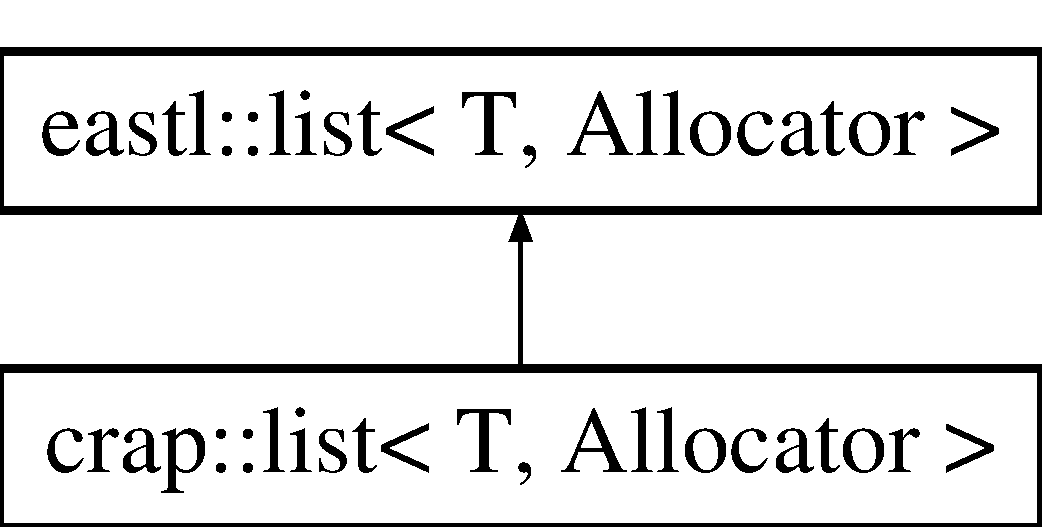
\includegraphics[height=2.000000cm]{classcrap_1_1list}
\end{center}
\end{figure}


The documentation for this class was generated from the following file\-:\begin{DoxyCompactItemize}
\item 
/mnt/windows/data/\-Programmierung/\-C\-R\-A\-P/src/crap/container/\hyperlink{list_8h}{list.\-h}\end{DoxyCompactItemize}

\hypertarget{classcrap_1_1math}{\section{crap\-:\-:math Class Reference}
\label{classcrap_1_1math}\index{crap\-::math@{crap\-::math}}
}


{\ttfamily \#include $<$math.\-h$>$}

\subsection*{Static Public Member Functions}
\begin{DoxyCompactItemize}
\item 
static \hyperlink{compilers_8h_a5a40526b8d842e7ff731509998bb0f1c}{C\-R\-A\-P\-\_\-\-I\-N\-L\-I\-N\-E} \hyperlink{types_8h_a154db6eda6a99565cb060a1da4b4c930}{f32} \hyperlink{classcrap_1_1math_a5055faf0d13c15d1eefaaa25a71ec783}{modf} (const \hyperlink{types_8h_a154db6eda6a99565cb060a1da4b4c930}{f32} \&x, \hyperlink{types_8h_a154db6eda6a99565cb060a1da4b4c930}{f32} $\ast$p)
\item 
static \hyperlink{compilers_8h_a5a40526b8d842e7ff731509998bb0f1c}{C\-R\-A\-P\-\_\-\-I\-N\-L\-I\-N\-E} \hyperlink{types_8h_a154db6eda6a99565cb060a1da4b4c930}{f32} \hyperlink{classcrap_1_1math_addea05390af4414d2b0eca120004b92d}{trunc} (const \hyperlink{types_8h_a154db6eda6a99565cb060a1da4b4c930}{f32} \&x)
\item 
static \hyperlink{compilers_8h_a5a40526b8d842e7ff731509998bb0f1c}{C\-R\-A\-P\-\_\-\-I\-N\-L\-I\-N\-E} \hyperlink{types_8h_a154db6eda6a99565cb060a1da4b4c930}{f32} \hyperlink{classcrap_1_1math_a5df2cde4c714d82fd372a083f36c7324}{frac} (const \hyperlink{types_8h_a154db6eda6a99565cb060a1da4b4c930}{f32} \&x)
\item 
static \hyperlink{compilers_8h_a5a40526b8d842e7ff731509998bb0f1c}{C\-R\-A\-P\-\_\-\-I\-N\-L\-I\-N\-E} \hyperlink{types_8h_a154db6eda6a99565cb060a1da4b4c930}{f32} \hyperlink{classcrap_1_1math_abd7ed0b391a065946d304acfbff17b3c}{fmod} (const \hyperlink{types_8h_a154db6eda6a99565cb060a1da4b4c930}{f32} \&x, const \hyperlink{types_8h_a154db6eda6a99565cb060a1da4b4c930}{f32} \&y)
\item 
static \hyperlink{compilers_8h_a5a40526b8d842e7ff731509998bb0f1c}{C\-R\-A\-P\-\_\-\-I\-N\-L\-I\-N\-E} \hyperlink{types_8h_a154db6eda6a99565cb060a1da4b4c930}{f32} \hyperlink{classcrap_1_1math_a78557527417d59dd3be3c27bb9cc041d}{drem} (const \hyperlink{types_8h_a154db6eda6a99565cb060a1da4b4c930}{f32} \&x, const \hyperlink{types_8h_a154db6eda6a99565cb060a1da4b4c930}{f32} \&y)
\item 
static \hyperlink{compilers_8h_a5a40526b8d842e7ff731509998bb0f1c}{C\-R\-A\-P\-\_\-\-I\-N\-L\-I\-N\-E} \hyperlink{types_8h_a154db6eda6a99565cb060a1da4b4c930}{f32} \hyperlink{classcrap_1_1math_a5b7b183b035126370b273097c3203f98}{wrap} (const \hyperlink{types_8h_a154db6eda6a99565cb060a1da4b4c930}{f32} \&x, const \hyperlink{types_8h_a154db6eda6a99565cb060a1da4b4c930}{f32} \&y)
\item 
static \hyperlink{compilers_8h_a5a40526b8d842e7ff731509998bb0f1c}{C\-R\-A\-P\-\_\-\-I\-N\-L\-I\-N\-E} \hyperlink{types_8h_a154db6eda6a99565cb060a1da4b4c930}{f32} \hyperlink{classcrap_1_1math_ad39054c4d325896b0037d51f40dcb3e3}{log2} (const \hyperlink{types_8h_a154db6eda6a99565cb060a1da4b4c930}{f32} \&x)
\item 
static \hyperlink{compilers_8h_a5a40526b8d842e7ff731509998bb0f1c}{C\-R\-A\-P\-\_\-\-I\-N\-L\-I\-N\-E} \hyperlink{types_8h_a154db6eda6a99565cb060a1da4b4c930}{f32} \hyperlink{classcrap_1_1math_a064d14a37a3e764e5c3b427d47a8e725}{log} (const \hyperlink{types_8h_a154db6eda6a99565cb060a1da4b4c930}{f32} \&x)
\item 
static \hyperlink{compilers_8h_a5a40526b8d842e7ff731509998bb0f1c}{C\-R\-A\-P\-\_\-\-I\-N\-L\-I\-N\-E} \hyperlink{types_8h_a154db6eda6a99565cb060a1da4b4c930}{f32} \hyperlink{classcrap_1_1math_a2971428e918a5a5515eacce5f36748a9}{exp2} (const \hyperlink{types_8h_a154db6eda6a99565cb060a1da4b4c930}{f32} \&x)
\item 
static \hyperlink{compilers_8h_a5a40526b8d842e7ff731509998bb0f1c}{C\-R\-A\-P\-\_\-\-I\-N\-L\-I\-N\-E} \hyperlink{types_8h_a154db6eda6a99565cb060a1da4b4c930}{f32} \hyperlink{classcrap_1_1math_adefd5c2329265c8c41c2d698f5be3321}{exp} (const \hyperlink{types_8h_a154db6eda6a99565cb060a1da4b4c930}{f32} \&x)
\item 
static \hyperlink{compilers_8h_a5a40526b8d842e7ff731509998bb0f1c}{C\-R\-A\-P\-\_\-\-I\-N\-L\-I\-N\-E} \hyperlink{types_8h_a154db6eda6a99565cb060a1da4b4c930}{f32} \hyperlink{classcrap_1_1math_af052f0b864810d1dbf16eb30e94f0d43}{pow} (const \hyperlink{types_8h_a154db6eda6a99565cb060a1da4b4c930}{f32} \&x, const \hyperlink{types_8h_a154db6eda6a99565cb060a1da4b4c930}{f32} \&y)
\item 
static \hyperlink{compilers_8h_a5a40526b8d842e7ff731509998bb0f1c}{C\-R\-A\-P\-\_\-\-I\-N\-L\-I\-N\-E} \hyperlink{types_8h_a154db6eda6a99565cb060a1da4b4c930}{f32} \hyperlink{classcrap_1_1math_a387a10534e5206369e1fae55023eb533}{cos} (const \hyperlink{types_8h_a154db6eda6a99565cb060a1da4b4c930}{f32} \&x)
\item 
static \hyperlink{compilers_8h_a5a40526b8d842e7ff731509998bb0f1c}{C\-R\-A\-P\-\_\-\-I\-N\-L\-I\-N\-E} \hyperlink{types_8h_a154db6eda6a99565cb060a1da4b4c930}{f32} \hyperlink{classcrap_1_1math_a8f0157711f1b633873795da39bb79af1}{sin} (const \hyperlink{types_8h_a154db6eda6a99565cb060a1da4b4c930}{f32} \&x)
\item 
static \hyperlink{compilers_8h_a5a40526b8d842e7ff731509998bb0f1c}{C\-R\-A\-P\-\_\-\-I\-N\-L\-I\-N\-E} void \hyperlink{classcrap_1_1math_adf742e2d86fb807a6a96da3223eb003e}{sincos} (const \hyperlink{types_8h_a154db6eda6a99565cb060a1da4b4c930}{f32} \&x, \hyperlink{types_8h_a154db6eda6a99565cb060a1da4b4c930}{f32} $\ast$s, \hyperlink{types_8h_a154db6eda6a99565cb060a1da4b4c930}{f32} $\ast$c)
\item 
static \hyperlink{compilers_8h_a5a40526b8d842e7ff731509998bb0f1c}{C\-R\-A\-P\-\_\-\-I\-N\-L\-I\-N\-E} \hyperlink{types_8h_a154db6eda6a99565cb060a1da4b4c930}{f32} \hyperlink{classcrap_1_1math_ae17c7f66d0fda534d03ab430518e4492}{tan} (const \hyperlink{types_8h_a154db6eda6a99565cb060a1da4b4c930}{f32} \&x)
\item 
static \hyperlink{compilers_8h_a5a40526b8d842e7ff731509998bb0f1c}{C\-R\-A\-P\-\_\-\-I\-N\-L\-I\-N\-E} \hyperlink{types_8h_a154db6eda6a99565cb060a1da4b4c930}{f32} \hyperlink{classcrap_1_1math_a02c923feb57285321866d6886f509c25}{cosh} (const \hyperlink{types_8h_a154db6eda6a99565cb060a1da4b4c930}{f32} \&x)
\item 
static \hyperlink{compilers_8h_a5a40526b8d842e7ff731509998bb0f1c}{C\-R\-A\-P\-\_\-\-I\-N\-L\-I\-N\-E} \hyperlink{types_8h_a154db6eda6a99565cb060a1da4b4c930}{f32} \hyperlink{classcrap_1_1math_acc79f62c7f592e3cd7af41bdba51dbca}{sinh} (const \hyperlink{types_8h_a154db6eda6a99565cb060a1da4b4c930}{f32} \&x)
\item 
static \hyperlink{compilers_8h_a5a40526b8d842e7ff731509998bb0f1c}{C\-R\-A\-P\-\_\-\-I\-N\-L\-I\-N\-E} \hyperlink{types_8h_a154db6eda6a99565cb060a1da4b4c930}{f32} \hyperlink{classcrap_1_1math_a4b929f1c2b7d09a1ff8e7e8026c18b7a}{tanh} (const \hyperlink{types_8h_a154db6eda6a99565cb060a1da4b4c930}{f32} \&x)
\item 
static \hyperlink{compilers_8h_a5a40526b8d842e7ff731509998bb0f1c}{C\-R\-A\-P\-\_\-\-I\-N\-L\-I\-N\-E} \hyperlink{types_8h_a154db6eda6a99565cb060a1da4b4c930}{f32} \hyperlink{classcrap_1_1math_a4badbf89510cb9ad5b8ce93268bbfc9f}{acos} (const \hyperlink{types_8h_a154db6eda6a99565cb060a1da4b4c930}{f32} \&x)
\item 
static \hyperlink{compilers_8h_a5a40526b8d842e7ff731509998bb0f1c}{C\-R\-A\-P\-\_\-\-I\-N\-L\-I\-N\-E} \hyperlink{types_8h_a154db6eda6a99565cb060a1da4b4c930}{f32} \hyperlink{classcrap_1_1math_a9b6dd7222bafbd9e50146890f18fc1d4}{asin} (const \hyperlink{types_8h_a154db6eda6a99565cb060a1da4b4c930}{f32} \&x)
\item 
static \hyperlink{compilers_8h_a5a40526b8d842e7ff731509998bb0f1c}{C\-R\-A\-P\-\_\-\-I\-N\-L\-I\-N\-E} \hyperlink{types_8h_a154db6eda6a99565cb060a1da4b4c930}{f32} \hyperlink{classcrap_1_1math_a0e1f655ac16d51675531c0a9529cc641}{atan2} (const \hyperlink{types_8h_a154db6eda6a99565cb060a1da4b4c930}{f32} \&y, const \hyperlink{types_8h_a154db6eda6a99565cb060a1da4b4c930}{f32} \&x)
\item 
static \hyperlink{compilers_8h_a5a40526b8d842e7ff731509998bb0f1c}{C\-R\-A\-P\-\_\-\-I\-N\-L\-I\-N\-E} \hyperlink{types_8h_a154db6eda6a99565cb060a1da4b4c930}{f32} \hyperlink{classcrap_1_1math_af8bdf37dc911e4a8c5c0ab9308bc3c7c}{atan} (const \hyperlink{types_8h_a154db6eda6a99565cb060a1da4b4c930}{f32} \&x)
\item 
static \hyperlink{compilers_8h_a5a40526b8d842e7ff731509998bb0f1c}{C\-R\-A\-P\-\_\-\-I\-N\-L\-I\-N\-E} \hyperlink{types_8h_a154db6eda6a99565cb060a1da4b4c930}{f32} \hyperlink{classcrap_1_1math_a08789ae66bd2c2c1c89ee699b94084f7}{acosh} (const \hyperlink{types_8h_a154db6eda6a99565cb060a1da4b4c930}{f32} \&x)
\item 
static \hyperlink{compilers_8h_a5a40526b8d842e7ff731509998bb0f1c}{C\-R\-A\-P\-\_\-\-I\-N\-L\-I\-N\-E} \hyperlink{types_8h_a154db6eda6a99565cb060a1da4b4c930}{f32} \hyperlink{classcrap_1_1math_a2f6427fa1838db06950127760fdef1e0}{asinh} (const \hyperlink{types_8h_a154db6eda6a99565cb060a1da4b4c930}{f32} \&x)
\item 
static \hyperlink{compilers_8h_a5a40526b8d842e7ff731509998bb0f1c}{C\-R\-A\-P\-\_\-\-I\-N\-L\-I\-N\-E} \hyperlink{types_8h_a154db6eda6a99565cb060a1da4b4c930}{f32} \hyperlink{classcrap_1_1math_ac90c2fe359767a341f8beca6d232df78}{atanh} (const \hyperlink{types_8h_a154db6eda6a99565cb060a1da4b4c930}{f32} \&x)
\end{DoxyCompactItemize}


\subsection{Member Function Documentation}
\hypertarget{classcrap_1_1math_a4badbf89510cb9ad5b8ce93268bbfc9f}{\index{crap\-::math@{crap\-::math}!acos@{acos}}
\index{acos@{acos}!crap::math@{crap\-::math}}
\subsubsection[{acos}]{\setlength{\rightskip}{0pt plus 5cm}static {\bf C\-R\-A\-P\-\_\-\-I\-N\-L\-I\-N\-E} {\bf f32} crap\-::math\-::acos (
\begin{DoxyParamCaption}
\item[{const {\bf f32} \&}]{x}
\end{DoxyParamCaption}
)\hspace{0.3cm}{\ttfamily [inline]}, {\ttfamily [static]}}}\label{classcrap_1_1math_a4badbf89510cb9ad5b8ce93268bbfc9f}
\hypertarget{classcrap_1_1math_a08789ae66bd2c2c1c89ee699b94084f7}{\index{crap\-::math@{crap\-::math}!acosh@{acosh}}
\index{acosh@{acosh}!crap::math@{crap\-::math}}
\subsubsection[{acosh}]{\setlength{\rightskip}{0pt plus 5cm}static {\bf C\-R\-A\-P\-\_\-\-I\-N\-L\-I\-N\-E} {\bf f32} crap\-::math\-::acosh (
\begin{DoxyParamCaption}
\item[{const {\bf f32} \&}]{x}
\end{DoxyParamCaption}
)\hspace{0.3cm}{\ttfamily [inline]}, {\ttfamily [static]}}}\label{classcrap_1_1math_a08789ae66bd2c2c1c89ee699b94084f7}
\hypertarget{classcrap_1_1math_a9b6dd7222bafbd9e50146890f18fc1d4}{\index{crap\-::math@{crap\-::math}!asin@{asin}}
\index{asin@{asin}!crap::math@{crap\-::math}}
\subsubsection[{asin}]{\setlength{\rightskip}{0pt plus 5cm}static {\bf C\-R\-A\-P\-\_\-\-I\-N\-L\-I\-N\-E} {\bf f32} crap\-::math\-::asin (
\begin{DoxyParamCaption}
\item[{const {\bf f32} \&}]{x}
\end{DoxyParamCaption}
)\hspace{0.3cm}{\ttfamily [inline]}, {\ttfamily [static]}}}\label{classcrap_1_1math_a9b6dd7222bafbd9e50146890f18fc1d4}
\hypertarget{classcrap_1_1math_a2f6427fa1838db06950127760fdef1e0}{\index{crap\-::math@{crap\-::math}!asinh@{asinh}}
\index{asinh@{asinh}!crap::math@{crap\-::math}}
\subsubsection[{asinh}]{\setlength{\rightskip}{0pt plus 5cm}static {\bf C\-R\-A\-P\-\_\-\-I\-N\-L\-I\-N\-E} {\bf f32} crap\-::math\-::asinh (
\begin{DoxyParamCaption}
\item[{const {\bf f32} \&}]{x}
\end{DoxyParamCaption}
)\hspace{0.3cm}{\ttfamily [inline]}, {\ttfamily [static]}}}\label{classcrap_1_1math_a2f6427fa1838db06950127760fdef1e0}
\hypertarget{classcrap_1_1math_af8bdf37dc911e4a8c5c0ab9308bc3c7c}{\index{crap\-::math@{crap\-::math}!atan@{atan}}
\index{atan@{atan}!crap::math@{crap\-::math}}
\subsubsection[{atan}]{\setlength{\rightskip}{0pt plus 5cm}static {\bf C\-R\-A\-P\-\_\-\-I\-N\-L\-I\-N\-E} {\bf f32} crap\-::math\-::atan (
\begin{DoxyParamCaption}
\item[{const {\bf f32} \&}]{x}
\end{DoxyParamCaption}
)\hspace{0.3cm}{\ttfamily [inline]}, {\ttfamily [static]}}}\label{classcrap_1_1math_af8bdf37dc911e4a8c5c0ab9308bc3c7c}
\hypertarget{classcrap_1_1math_a0e1f655ac16d51675531c0a9529cc641}{\index{crap\-::math@{crap\-::math}!atan2@{atan2}}
\index{atan2@{atan2}!crap::math@{crap\-::math}}
\subsubsection[{atan2}]{\setlength{\rightskip}{0pt plus 5cm}static {\bf C\-R\-A\-P\-\_\-\-I\-N\-L\-I\-N\-E} {\bf f32} crap\-::math\-::atan2 (
\begin{DoxyParamCaption}
\item[{const {\bf f32} \&}]{y, }
\item[{const {\bf f32} \&}]{x}
\end{DoxyParamCaption}
)\hspace{0.3cm}{\ttfamily [inline]}, {\ttfamily [static]}}}\label{classcrap_1_1math_a0e1f655ac16d51675531c0a9529cc641}
\hypertarget{classcrap_1_1math_ac90c2fe359767a341f8beca6d232df78}{\index{crap\-::math@{crap\-::math}!atanh@{atanh}}
\index{atanh@{atanh}!crap::math@{crap\-::math}}
\subsubsection[{atanh}]{\setlength{\rightskip}{0pt plus 5cm}static {\bf C\-R\-A\-P\-\_\-\-I\-N\-L\-I\-N\-E} {\bf f32} crap\-::math\-::atanh (
\begin{DoxyParamCaption}
\item[{const {\bf f32} \&}]{x}
\end{DoxyParamCaption}
)\hspace{0.3cm}{\ttfamily [inline]}, {\ttfamily [static]}}}\label{classcrap_1_1math_ac90c2fe359767a341f8beca6d232df78}
\hypertarget{classcrap_1_1math_a387a10534e5206369e1fae55023eb533}{\index{crap\-::math@{crap\-::math}!cos@{cos}}
\index{cos@{cos}!crap::math@{crap\-::math}}
\subsubsection[{cos}]{\setlength{\rightskip}{0pt plus 5cm}static {\bf C\-R\-A\-P\-\_\-\-I\-N\-L\-I\-N\-E} {\bf f32} crap\-::math\-::cos (
\begin{DoxyParamCaption}
\item[{const {\bf f32} \&}]{x}
\end{DoxyParamCaption}
)\hspace{0.3cm}{\ttfamily [inline]}, {\ttfamily [static]}}}\label{classcrap_1_1math_a387a10534e5206369e1fae55023eb533}
\hypertarget{classcrap_1_1math_a02c923feb57285321866d6886f509c25}{\index{crap\-::math@{crap\-::math}!cosh@{cosh}}
\index{cosh@{cosh}!crap::math@{crap\-::math}}
\subsubsection[{cosh}]{\setlength{\rightskip}{0pt plus 5cm}static {\bf C\-R\-A\-P\-\_\-\-I\-N\-L\-I\-N\-E} {\bf f32} crap\-::math\-::cosh (
\begin{DoxyParamCaption}
\item[{const {\bf f32} \&}]{x}
\end{DoxyParamCaption}
)\hspace{0.3cm}{\ttfamily [inline]}, {\ttfamily [static]}}}\label{classcrap_1_1math_a02c923feb57285321866d6886f509c25}
\hypertarget{classcrap_1_1math_a78557527417d59dd3be3c27bb9cc041d}{\index{crap\-::math@{crap\-::math}!drem@{drem}}
\index{drem@{drem}!crap::math@{crap\-::math}}
\subsubsection[{drem}]{\setlength{\rightskip}{0pt plus 5cm}static {\bf C\-R\-A\-P\-\_\-\-I\-N\-L\-I\-N\-E} {\bf f32} crap\-::math\-::drem (
\begin{DoxyParamCaption}
\item[{const {\bf f32} \&}]{x, }
\item[{const {\bf f32} \&}]{y}
\end{DoxyParamCaption}
)\hspace{0.3cm}{\ttfamily [inline]}, {\ttfamily [static]}}}\label{classcrap_1_1math_a78557527417d59dd3be3c27bb9cc041d}
\hypertarget{classcrap_1_1math_adefd5c2329265c8c41c2d698f5be3321}{\index{crap\-::math@{crap\-::math}!exp@{exp}}
\index{exp@{exp}!crap::math@{crap\-::math}}
\subsubsection[{exp}]{\setlength{\rightskip}{0pt plus 5cm}static {\bf C\-R\-A\-P\-\_\-\-I\-N\-L\-I\-N\-E} {\bf f32} crap\-::math\-::exp (
\begin{DoxyParamCaption}
\item[{const {\bf f32} \&}]{x}
\end{DoxyParamCaption}
)\hspace{0.3cm}{\ttfamily [inline]}, {\ttfamily [static]}}}\label{classcrap_1_1math_adefd5c2329265c8c41c2d698f5be3321}
\hypertarget{classcrap_1_1math_a2971428e918a5a5515eacce5f36748a9}{\index{crap\-::math@{crap\-::math}!exp2@{exp2}}
\index{exp2@{exp2}!crap::math@{crap\-::math}}
\subsubsection[{exp2}]{\setlength{\rightskip}{0pt plus 5cm}static {\bf C\-R\-A\-P\-\_\-\-I\-N\-L\-I\-N\-E} {\bf f32} crap\-::math\-::exp2 (
\begin{DoxyParamCaption}
\item[{const {\bf f32} \&}]{x}
\end{DoxyParamCaption}
)\hspace{0.3cm}{\ttfamily [inline]}, {\ttfamily [static]}}}\label{classcrap_1_1math_a2971428e918a5a5515eacce5f36748a9}
\hypertarget{classcrap_1_1math_abd7ed0b391a065946d304acfbff17b3c}{\index{crap\-::math@{crap\-::math}!fmod@{fmod}}
\index{fmod@{fmod}!crap::math@{crap\-::math}}
\subsubsection[{fmod}]{\setlength{\rightskip}{0pt plus 5cm}static {\bf C\-R\-A\-P\-\_\-\-I\-N\-L\-I\-N\-E} {\bf f32} crap\-::math\-::fmod (
\begin{DoxyParamCaption}
\item[{const {\bf f32} \&}]{x, }
\item[{const {\bf f32} \&}]{y}
\end{DoxyParamCaption}
)\hspace{0.3cm}{\ttfamily [inline]}, {\ttfamily [static]}}}\label{classcrap_1_1math_abd7ed0b391a065946d304acfbff17b3c}
\hypertarget{classcrap_1_1math_a5df2cde4c714d82fd372a083f36c7324}{\index{crap\-::math@{crap\-::math}!frac@{frac}}
\index{frac@{frac}!crap::math@{crap\-::math}}
\subsubsection[{frac}]{\setlength{\rightskip}{0pt plus 5cm}static {\bf C\-R\-A\-P\-\_\-\-I\-N\-L\-I\-N\-E} {\bf f32} crap\-::math\-::frac (
\begin{DoxyParamCaption}
\item[{const {\bf f32} \&}]{x}
\end{DoxyParamCaption}
)\hspace{0.3cm}{\ttfamily [inline]}, {\ttfamily [static]}}}\label{classcrap_1_1math_a5df2cde4c714d82fd372a083f36c7324}
\hypertarget{classcrap_1_1math_a064d14a37a3e764e5c3b427d47a8e725}{\index{crap\-::math@{crap\-::math}!log@{log}}
\index{log@{log}!crap::math@{crap\-::math}}
\subsubsection[{log}]{\setlength{\rightskip}{0pt plus 5cm}static {\bf C\-R\-A\-P\-\_\-\-I\-N\-L\-I\-N\-E} {\bf f32} crap\-::math\-::log (
\begin{DoxyParamCaption}
\item[{const {\bf f32} \&}]{x}
\end{DoxyParamCaption}
)\hspace{0.3cm}{\ttfamily [inline]}, {\ttfamily [static]}}}\label{classcrap_1_1math_a064d14a37a3e764e5c3b427d47a8e725}
\hypertarget{classcrap_1_1math_ad39054c4d325896b0037d51f40dcb3e3}{\index{crap\-::math@{crap\-::math}!log2@{log2}}
\index{log2@{log2}!crap::math@{crap\-::math}}
\subsubsection[{log2}]{\setlength{\rightskip}{0pt plus 5cm}static {\bf C\-R\-A\-P\-\_\-\-I\-N\-L\-I\-N\-E} {\bf f32} crap\-::math\-::log2 (
\begin{DoxyParamCaption}
\item[{const {\bf f32} \&}]{x}
\end{DoxyParamCaption}
)\hspace{0.3cm}{\ttfamily [inline]}, {\ttfamily [static]}}}\label{classcrap_1_1math_ad39054c4d325896b0037d51f40dcb3e3}
\hypertarget{classcrap_1_1math_a5055faf0d13c15d1eefaaa25a71ec783}{\index{crap\-::math@{crap\-::math}!modf@{modf}}
\index{modf@{modf}!crap::math@{crap\-::math}}
\subsubsection[{modf}]{\setlength{\rightskip}{0pt plus 5cm}static {\bf C\-R\-A\-P\-\_\-\-I\-N\-L\-I\-N\-E} {\bf f32} crap\-::math\-::modf (
\begin{DoxyParamCaption}
\item[{const {\bf f32} \&}]{x, }
\item[{{\bf f32} $\ast$}]{p}
\end{DoxyParamCaption}
)\hspace{0.3cm}{\ttfamily [inline]}, {\ttfamily [static]}}}\label{classcrap_1_1math_a5055faf0d13c15d1eefaaa25a71ec783}
\hypertarget{classcrap_1_1math_af052f0b864810d1dbf16eb30e94f0d43}{\index{crap\-::math@{crap\-::math}!pow@{pow}}
\index{pow@{pow}!crap::math@{crap\-::math}}
\subsubsection[{pow}]{\setlength{\rightskip}{0pt plus 5cm}static {\bf C\-R\-A\-P\-\_\-\-I\-N\-L\-I\-N\-E} {\bf f32} crap\-::math\-::pow (
\begin{DoxyParamCaption}
\item[{const {\bf f32} \&}]{x, }
\item[{const {\bf f32} \&}]{y}
\end{DoxyParamCaption}
)\hspace{0.3cm}{\ttfamily [inline]}, {\ttfamily [static]}}}\label{classcrap_1_1math_af052f0b864810d1dbf16eb30e94f0d43}
\hypertarget{classcrap_1_1math_a8f0157711f1b633873795da39bb79af1}{\index{crap\-::math@{crap\-::math}!sin@{sin}}
\index{sin@{sin}!crap::math@{crap\-::math}}
\subsubsection[{sin}]{\setlength{\rightskip}{0pt plus 5cm}static {\bf C\-R\-A\-P\-\_\-\-I\-N\-L\-I\-N\-E} {\bf f32} crap\-::math\-::sin (
\begin{DoxyParamCaption}
\item[{const {\bf f32} \&}]{x}
\end{DoxyParamCaption}
)\hspace{0.3cm}{\ttfamily [inline]}, {\ttfamily [static]}}}\label{classcrap_1_1math_a8f0157711f1b633873795da39bb79af1}
\hypertarget{classcrap_1_1math_adf742e2d86fb807a6a96da3223eb003e}{\index{crap\-::math@{crap\-::math}!sincos@{sincos}}
\index{sincos@{sincos}!crap::math@{crap\-::math}}
\subsubsection[{sincos}]{\setlength{\rightskip}{0pt plus 5cm}static {\bf C\-R\-A\-P\-\_\-\-I\-N\-L\-I\-N\-E} void crap\-::math\-::sincos (
\begin{DoxyParamCaption}
\item[{const {\bf f32} \&}]{x, }
\item[{{\bf f32} $\ast$}]{s, }
\item[{{\bf f32} $\ast$}]{c}
\end{DoxyParamCaption}
)\hspace{0.3cm}{\ttfamily [inline]}, {\ttfamily [static]}}}\label{classcrap_1_1math_adf742e2d86fb807a6a96da3223eb003e}
\hypertarget{classcrap_1_1math_acc79f62c7f592e3cd7af41bdba51dbca}{\index{crap\-::math@{crap\-::math}!sinh@{sinh}}
\index{sinh@{sinh}!crap::math@{crap\-::math}}
\subsubsection[{sinh}]{\setlength{\rightskip}{0pt plus 5cm}static {\bf C\-R\-A\-P\-\_\-\-I\-N\-L\-I\-N\-E} {\bf f32} crap\-::math\-::sinh (
\begin{DoxyParamCaption}
\item[{const {\bf f32} \&}]{x}
\end{DoxyParamCaption}
)\hspace{0.3cm}{\ttfamily [inline]}, {\ttfamily [static]}}}\label{classcrap_1_1math_acc79f62c7f592e3cd7af41bdba51dbca}
\hypertarget{classcrap_1_1math_ae17c7f66d0fda534d03ab430518e4492}{\index{crap\-::math@{crap\-::math}!tan@{tan}}
\index{tan@{tan}!crap::math@{crap\-::math}}
\subsubsection[{tan}]{\setlength{\rightskip}{0pt plus 5cm}static {\bf C\-R\-A\-P\-\_\-\-I\-N\-L\-I\-N\-E} {\bf f32} crap\-::math\-::tan (
\begin{DoxyParamCaption}
\item[{const {\bf f32} \&}]{x}
\end{DoxyParamCaption}
)\hspace{0.3cm}{\ttfamily [inline]}, {\ttfamily [static]}}}\label{classcrap_1_1math_ae17c7f66d0fda534d03ab430518e4492}
\hypertarget{classcrap_1_1math_a4b929f1c2b7d09a1ff8e7e8026c18b7a}{\index{crap\-::math@{crap\-::math}!tanh@{tanh}}
\index{tanh@{tanh}!crap::math@{crap\-::math}}
\subsubsection[{tanh}]{\setlength{\rightskip}{0pt plus 5cm}static {\bf C\-R\-A\-P\-\_\-\-I\-N\-L\-I\-N\-E} {\bf f32} crap\-::math\-::tanh (
\begin{DoxyParamCaption}
\item[{const {\bf f32} \&}]{x}
\end{DoxyParamCaption}
)\hspace{0.3cm}{\ttfamily [inline]}, {\ttfamily [static]}}}\label{classcrap_1_1math_a4b929f1c2b7d09a1ff8e7e8026c18b7a}
\hypertarget{classcrap_1_1math_addea05390af4414d2b0eca120004b92d}{\index{crap\-::math@{crap\-::math}!trunc@{trunc}}
\index{trunc@{trunc}!crap::math@{crap\-::math}}
\subsubsection[{trunc}]{\setlength{\rightskip}{0pt plus 5cm}static {\bf C\-R\-A\-P\-\_\-\-I\-N\-L\-I\-N\-E} {\bf f32} crap\-::math\-::trunc (
\begin{DoxyParamCaption}
\item[{const {\bf f32} \&}]{x}
\end{DoxyParamCaption}
)\hspace{0.3cm}{\ttfamily [inline]}, {\ttfamily [static]}}}\label{classcrap_1_1math_addea05390af4414d2b0eca120004b92d}
\hypertarget{classcrap_1_1math_a5b7b183b035126370b273097c3203f98}{\index{crap\-::math@{crap\-::math}!wrap@{wrap}}
\index{wrap@{wrap}!crap::math@{crap\-::math}}
\subsubsection[{wrap}]{\setlength{\rightskip}{0pt plus 5cm}static {\bf C\-R\-A\-P\-\_\-\-I\-N\-L\-I\-N\-E} {\bf f32} crap\-::math\-::wrap (
\begin{DoxyParamCaption}
\item[{const {\bf f32} \&}]{x, }
\item[{const {\bf f32} \&}]{y}
\end{DoxyParamCaption}
)\hspace{0.3cm}{\ttfamily [inline]}, {\ttfamily [static]}}}\label{classcrap_1_1math_a5b7b183b035126370b273097c3203f98}


The documentation for this class was generated from the following file\-:\begin{DoxyCompactItemize}
\item 
/mnt/windows/data/\-Programmierung/\-C\-R\-A\-P/src/crap/math/\hyperlink{math_2math_8h}{math.\-h}\end{DoxyCompactItemize}

\hypertarget{classcrap_1_1memory__pool}{\section{crap\-:\-:memory\-\_\-pool Class Reference}
\label{classcrap_1_1memory__pool}\index{crap\-::memory\-\_\-pool@{crap\-::memory\-\_\-pool}}
}


{\ttfamily \#include $<$memorypool.\-h$>$}

\subsection*{Public Member Functions}
\begin{DoxyCompactItemize}
\item 
\hyperlink{classcrap_1_1memory__pool_a1737ff4849d880063e5e29149753b16c}{memory\-\_\-pool} (void)
\begin{DoxyCompactList}\small\item\em default constructor \end{DoxyCompactList}\item 
\hyperlink{classcrap_1_1memory__pool_a66bd906710927e8e3c3ad66003eae84d}{memory\-\_\-pool} (\hyperlink{types_8h_a38c0a12279ffe0fabec44939e753c914}{size\-\_\-t32} \hyperlink{classcrap_1_1memory__pool_adb17e01142872367d7451c4e9ce19cef}{size})
\begin{DoxyCompactList}\small\item\em constructor with initial size \end{DoxyCompactList}\item 
\hyperlink{classcrap_1_1memory__pool_ac9c5827710ea2e286081ccf215de18c8}{$\sim$memory\-\_\-pool} (void)
\begin{DoxyCompactList}\small\item\em destructor \end{DoxyCompactList}\item 
void \hyperlink{classcrap_1_1memory__pool_a406348dc0a371f3a524d109f2a7e00f4}{init} (\hyperlink{types_8h_a38c0a12279ffe0fabec44939e753c914}{size\-\_\-t32} \hyperlink{classcrap_1_1memory__pool_adb17e01142872367d7451c4e9ce19cef}{size})
\begin{DoxyCompactList}\small\item\em initializing function -\/ when default constructor was used \end{DoxyCompactList}\item 
void $\ast$ \hyperlink{classcrap_1_1memory__pool_aae96e27b836c75fa42ad3a9973726553}{allocate} (\hyperlink{types_8h_a38c0a12279ffe0fabec44939e753c914}{size\-\_\-t32} \hyperlink{classcrap_1_1memory__pool_adb17e01142872367d7451c4e9ce19cef}{size})
\begin{DoxyCompactList}\small\item\em allocate specific amount of bytes \end{DoxyCompactList}\item 
void $\ast$ \hyperlink{classcrap_1_1memory__pool_a2bae67eb417ac2106964fb158a3b8289}{quick\-\_\-allocate} (\hyperlink{types_8h_a38c0a12279ffe0fabec44939e753c914}{size\-\_\-t32} \hyperlink{classcrap_1_1memory__pool_adb17e01142872367d7451c4e9ce19cef}{size})
\begin{DoxyCompactList}\small\item\em allocate quickly by using biggest free block pointer \end{DoxyCompactList}\item 
void \hyperlink{classcrap_1_1memory__pool_a9535c7027e4bbd89bb763ab461080ac1}{deallocate} (void $\ast$address)
\begin{DoxyCompactList}\small\item\em deallocating memory, by taking header out of list \end{DoxyCompactList}\item 
void $\ast$ \hyperlink{classcrap_1_1memory__pool_a595f6e669ec14642431e7bd20b2a3b1d}{block\-\_\-start} (void) const 
\begin{DoxyCompactList}\small\item\em returns void pointer on first block \end{DoxyCompactList}\item 
\hyperlink{types_8h_a38c0a12279ffe0fabec44939e753c914}{size\-\_\-t32} \hyperlink{classcrap_1_1memory__pool_abc7e2a4dcba0c9207292a1778f157436}{total\-\_\-size} (void) const 
\begin{DoxyCompactList}\small\item\em returns total size \end{DoxyCompactList}\item 
\hyperlink{types_8h_a38c0a12279ffe0fabec44939e753c914}{size\-\_\-t32} \hyperlink{classcrap_1_1memory__pool_adb17e01142872367d7451c4e9ce19cef}{size} (void) const 
\begin{DoxyCompactList}\small\item\em returns current free space in pool (at all) \end{DoxyCompactList}\item 
\hyperlink{types_8h_a38c0a12279ffe0fabec44939e753c914}{size\-\_\-t32} \hyperlink{classcrap_1_1memory__pool_acaf9502477bb3130b92bab7f9cf4579f}{biggest\-\_\-block} (void) const 
\begin{DoxyCompactList}\small\item\em return size of biggest block (free memory) \end{DoxyCompactList}\item 
bool \hyperlink{classcrap_1_1memory__pool_ad01cbb03dc6aaed343e2160221a1266b}{is\-\_\-in\-\_\-range} (void $\ast$address) const 
\begin{DoxyCompactList}\small\item\em test if a pointer is in this pool \end{DoxyCompactList}\end{DoxyCompactItemize}


\subsection{Constructor \& Destructor Documentation}
\hypertarget{classcrap_1_1memory__pool_a1737ff4849d880063e5e29149753b16c}{\index{crap\-::memory\-\_\-pool@{crap\-::memory\-\_\-pool}!memory\-\_\-pool@{memory\-\_\-pool}}
\index{memory\-\_\-pool@{memory\-\_\-pool}!crap::memory_pool@{crap\-::memory\-\_\-pool}}
\subsubsection[{memory\-\_\-pool}]{\setlength{\rightskip}{0pt plus 5cm}crap\-::memory\-\_\-pool\-::memory\-\_\-pool (
\begin{DoxyParamCaption}
\item[{void}]{}
\end{DoxyParamCaption}
)}}\label{classcrap_1_1memory__pool_a1737ff4849d880063e5e29149753b16c}


default constructor 

\hypertarget{classcrap_1_1memory__pool_a66bd906710927e8e3c3ad66003eae84d}{\index{crap\-::memory\-\_\-pool@{crap\-::memory\-\_\-pool}!memory\-\_\-pool@{memory\-\_\-pool}}
\index{memory\-\_\-pool@{memory\-\_\-pool}!crap::memory_pool@{crap\-::memory\-\_\-pool}}
\subsubsection[{memory\-\_\-pool}]{\setlength{\rightskip}{0pt plus 5cm}crap\-::memory\-\_\-pool\-::memory\-\_\-pool (
\begin{DoxyParamCaption}
\item[{{\bf size\-\_\-t32}}]{size}
\end{DoxyParamCaption}
)}}\label{classcrap_1_1memory__pool_a66bd906710927e8e3c3ad66003eae84d}


constructor with initial size 

\hypertarget{classcrap_1_1memory__pool_ac9c5827710ea2e286081ccf215de18c8}{\index{crap\-::memory\-\_\-pool@{crap\-::memory\-\_\-pool}!$\sim$memory\-\_\-pool@{$\sim$memory\-\_\-pool}}
\index{$\sim$memory\-\_\-pool@{$\sim$memory\-\_\-pool}!crap::memory_pool@{crap\-::memory\-\_\-pool}}
\subsubsection[{$\sim$memory\-\_\-pool}]{\setlength{\rightskip}{0pt plus 5cm}crap\-::memory\-\_\-pool\-::$\sim$memory\-\_\-pool (
\begin{DoxyParamCaption}
\item[{void}]{}
\end{DoxyParamCaption}
)}}\label{classcrap_1_1memory__pool_ac9c5827710ea2e286081ccf215de18c8}


destructor 



\subsection{Member Function Documentation}
\hypertarget{classcrap_1_1memory__pool_aae96e27b836c75fa42ad3a9973726553}{\index{crap\-::memory\-\_\-pool@{crap\-::memory\-\_\-pool}!allocate@{allocate}}
\index{allocate@{allocate}!crap::memory_pool@{crap\-::memory\-\_\-pool}}
\subsubsection[{allocate}]{\setlength{\rightskip}{0pt plus 5cm}void $\ast$ crap\-::memory\-\_\-pool\-::allocate (
\begin{DoxyParamCaption}
\item[{{\bf size\-\_\-t32}}]{size}
\end{DoxyParamCaption}
)\hspace{0.3cm}{\ttfamily [inline]}}}\label{classcrap_1_1memory__pool_aae96e27b836c75fa42ad3a9973726553}


allocate specific amount of bytes 

\hypertarget{classcrap_1_1memory__pool_acaf9502477bb3130b92bab7f9cf4579f}{\index{crap\-::memory\-\_\-pool@{crap\-::memory\-\_\-pool}!biggest\-\_\-block@{biggest\-\_\-block}}
\index{biggest\-\_\-block@{biggest\-\_\-block}!crap::memory_pool@{crap\-::memory\-\_\-pool}}
\subsubsection[{biggest\-\_\-block}]{\setlength{\rightskip}{0pt plus 5cm}{\bf size\-\_\-t32} crap\-::memory\-\_\-pool\-::biggest\-\_\-block (
\begin{DoxyParamCaption}
\item[{void}]{}
\end{DoxyParamCaption}
) const\hspace{0.3cm}{\ttfamily [inline]}}}\label{classcrap_1_1memory__pool_acaf9502477bb3130b92bab7f9cf4579f}


return size of biggest block (free memory) 

\hypertarget{classcrap_1_1memory__pool_a595f6e669ec14642431e7bd20b2a3b1d}{\index{crap\-::memory\-\_\-pool@{crap\-::memory\-\_\-pool}!block\-\_\-start@{block\-\_\-start}}
\index{block\-\_\-start@{block\-\_\-start}!crap::memory_pool@{crap\-::memory\-\_\-pool}}
\subsubsection[{block\-\_\-start}]{\setlength{\rightskip}{0pt plus 5cm}void$\ast$ crap\-::memory\-\_\-pool\-::block\-\_\-start (
\begin{DoxyParamCaption}
\item[{void}]{}
\end{DoxyParamCaption}
) const\hspace{0.3cm}{\ttfamily [inline]}}}\label{classcrap_1_1memory__pool_a595f6e669ec14642431e7bd20b2a3b1d}


returns void pointer on first block 

\hypertarget{classcrap_1_1memory__pool_a9535c7027e4bbd89bb763ab461080ac1}{\index{crap\-::memory\-\_\-pool@{crap\-::memory\-\_\-pool}!deallocate@{deallocate}}
\index{deallocate@{deallocate}!crap::memory_pool@{crap\-::memory\-\_\-pool}}
\subsubsection[{deallocate}]{\setlength{\rightskip}{0pt plus 5cm}void crap\-::memory\-\_\-pool\-::deallocate (
\begin{DoxyParamCaption}
\item[{void $\ast$}]{address}
\end{DoxyParamCaption}
)\hspace{0.3cm}{\ttfamily [inline]}}}\label{classcrap_1_1memory__pool_a9535c7027e4bbd89bb763ab461080ac1}


deallocating memory, by taking header out of list 

\hypertarget{classcrap_1_1memory__pool_a406348dc0a371f3a524d109f2a7e00f4}{\index{crap\-::memory\-\_\-pool@{crap\-::memory\-\_\-pool}!init@{init}}
\index{init@{init}!crap::memory_pool@{crap\-::memory\-\_\-pool}}
\subsubsection[{init}]{\setlength{\rightskip}{0pt plus 5cm}void crap\-::memory\-\_\-pool\-::init (
\begin{DoxyParamCaption}
\item[{{\bf size\-\_\-t32}}]{size}
\end{DoxyParamCaption}
)\hspace{0.3cm}{\ttfamily [inline]}}}\label{classcrap_1_1memory__pool_a406348dc0a371f3a524d109f2a7e00f4}


initializing function -\/ when default constructor was used 

\hypertarget{classcrap_1_1memory__pool_ad01cbb03dc6aaed343e2160221a1266b}{\index{crap\-::memory\-\_\-pool@{crap\-::memory\-\_\-pool}!is\-\_\-in\-\_\-range@{is\-\_\-in\-\_\-range}}
\index{is\-\_\-in\-\_\-range@{is\-\_\-in\-\_\-range}!crap::memory_pool@{crap\-::memory\-\_\-pool}}
\subsubsection[{is\-\_\-in\-\_\-range}]{\setlength{\rightskip}{0pt plus 5cm}bool crap\-::memory\-\_\-pool\-::is\-\_\-in\-\_\-range (
\begin{DoxyParamCaption}
\item[{void $\ast$}]{address}
\end{DoxyParamCaption}
) const\hspace{0.3cm}{\ttfamily [inline]}}}\label{classcrap_1_1memory__pool_ad01cbb03dc6aaed343e2160221a1266b}


test if a pointer is in this pool 

\hypertarget{classcrap_1_1memory__pool_a2bae67eb417ac2106964fb158a3b8289}{\index{crap\-::memory\-\_\-pool@{crap\-::memory\-\_\-pool}!quick\-\_\-allocate@{quick\-\_\-allocate}}
\index{quick\-\_\-allocate@{quick\-\_\-allocate}!crap::memory_pool@{crap\-::memory\-\_\-pool}}
\subsubsection[{quick\-\_\-allocate}]{\setlength{\rightskip}{0pt plus 5cm}void $\ast$ crap\-::memory\-\_\-pool\-::quick\-\_\-allocate (
\begin{DoxyParamCaption}
\item[{{\bf size\-\_\-t32}}]{size}
\end{DoxyParamCaption}
)\hspace{0.3cm}{\ttfamily [inline]}}}\label{classcrap_1_1memory__pool_a2bae67eb417ac2106964fb158a3b8289}


allocate quickly by using biggest free block pointer 

\hypertarget{classcrap_1_1memory__pool_adb17e01142872367d7451c4e9ce19cef}{\index{crap\-::memory\-\_\-pool@{crap\-::memory\-\_\-pool}!size@{size}}
\index{size@{size}!crap::memory_pool@{crap\-::memory\-\_\-pool}}
\subsubsection[{size}]{\setlength{\rightskip}{0pt plus 5cm}{\bf size\-\_\-t32} crap\-::memory\-\_\-pool\-::size (
\begin{DoxyParamCaption}
\item[{void}]{}
\end{DoxyParamCaption}
) const\hspace{0.3cm}{\ttfamily [inline]}}}\label{classcrap_1_1memory__pool_adb17e01142872367d7451c4e9ce19cef}


returns current free space in pool (at all) 

\hypertarget{classcrap_1_1memory__pool_abc7e2a4dcba0c9207292a1778f157436}{\index{crap\-::memory\-\_\-pool@{crap\-::memory\-\_\-pool}!total\-\_\-size@{total\-\_\-size}}
\index{total\-\_\-size@{total\-\_\-size}!crap::memory_pool@{crap\-::memory\-\_\-pool}}
\subsubsection[{total\-\_\-size}]{\setlength{\rightskip}{0pt plus 5cm}{\bf size\-\_\-t32} crap\-::memory\-\_\-pool\-::total\-\_\-size (
\begin{DoxyParamCaption}
\item[{void}]{}
\end{DoxyParamCaption}
) const\hspace{0.3cm}{\ttfamily [inline]}}}\label{classcrap_1_1memory__pool_abc7e2a4dcba0c9207292a1778f157436}


returns total size 



The documentation for this class was generated from the following file\-:\begin{DoxyCompactItemize}
\item 
/mnt/windows/data/\-Programmierung/\-C\-R\-A\-P/src/crap/memory/\hyperlink{memorypool_8h}{memorypool.\-h}\end{DoxyCompactItemize}

\hypertarget{classcrap_1_1_memory_tracker}{\section{crap\-:\-:Memory\-Tracker Class Reference}
\label{classcrap_1_1_memory_tracker}\index{crap\-::\-Memory\-Tracker@{crap\-::\-Memory\-Tracker}}
}


{\ttfamily \#include $<$memorytracker.\-h$>$}

\subsection*{Public Member Functions}
\begin{DoxyCompactItemize}
\item 
\hyperlink{classcrap_1_1_memory_tracker_ab0716dd893a69e436d13518839877928}{$\sim$\-Memory\-Tracker} (void)
\item 
void \hyperlink{classcrap_1_1_memory_tracker_a4359d60246c81633dcf7edb54cdb3ccd}{add\-Allocated\-Block} (\hyperlink{types_8h_a3f7e2bcbb0b4c338f3c4f6c937cd4234}{u64} size)
\item 
void \hyperlink{classcrap_1_1_memory_tracker_a31f0bd063637de46cbd50f687e3d8483}{remove\-Allocated\-Block} (\hyperlink{types_8h_a3f7e2bcbb0b4c338f3c4f6c937cd4234}{u64} size)
\item 
\hyperlink{types_8h_a3f7e2bcbb0b4c338f3c4f6c937cd4234}{u64} \hyperlink{classcrap_1_1_memory_tracker_af3493ef0fb8265b0995ef383c4b6e315}{allocated\-Memory\-Blocks} (void) const 
\item 
\hyperlink{types_8h_a3f7e2bcbb0b4c338f3c4f6c937cd4234}{u64} \hyperlink{classcrap_1_1_memory_tracker_a497bf283bd00573c40f19425e5294adb}{allocated\-Memory\-Blocks\-Max} (void) const 
\item 
\hyperlink{types_8h_a3f7e2bcbb0b4c338f3c4f6c937cd4234}{u64} \hyperlink{classcrap_1_1_memory_tracker_ab4a38fc8d81ae8c55c31d00d0572d31a}{allocated\-Memory\-Blocks\-All} (void) const 
\item 
\hyperlink{types_8h_a3f7e2bcbb0b4c338f3c4f6c937cd4234}{u64} \hyperlink{classcrap_1_1_memory_tracker_a65c6e6cf6a62252c0307c1d47c7ada84}{allocated\-Memory\-Blocks\-Mem} (void) const 
\item 
\hyperlink{types_8h_a3f7e2bcbb0b4c338f3c4f6c937cd4234}{u64} \hyperlink{classcrap_1_1_memory_tracker_ab8df5a98ac88d6043f21093610c213a1}{allocated\-Memory\-Blocks\-Mem\-Max} (void) const 
\item 
\hyperlink{types_8h_a3f7e2bcbb0b4c338f3c4f6c937cd4234}{u64} \hyperlink{classcrap_1_1_memory_tracker_a6277601119cc6039efbf811c32aa3a49}{allocated\-Memory\-Blocks\-Big} (void) const 
\item 
void \hyperlink{classcrap_1_1_memory_tracker_a8fef331c83bae77fb2d24c75d94384a1}{add\-Used\-Memory} (\hyperlink{types_8h_a3f7e2bcbb0b4c338f3c4f6c937cd4234}{u64} size)
\item 
void \hyperlink{classcrap_1_1_memory_tracker_af9205749a325944636967faf56fbf638}{remove\-Used\-Memory} (\hyperlink{types_8h_a3f7e2bcbb0b4c338f3c4f6c937cd4234}{u64} size)
\item 
\hyperlink{types_8h_a3f7e2bcbb0b4c338f3c4f6c937cd4234}{u64} \hyperlink{classcrap_1_1_memory_tracker_a684b98c04f08059b67b17d7946a5c412}{used\-Memory} (void) const 
\item 
\hyperlink{types_8h_a3f7e2bcbb0b4c338f3c4f6c937cd4234}{u64} \hyperlink{classcrap_1_1_memory_tracker_ab4f0406dea8cf0ab17d448677ab4400c}{used\-Memory\-Max} (void) const 
\item 
\hyperlink{types_8h_a3f7e2bcbb0b4c338f3c4f6c937cd4234}{u64} \hyperlink{classcrap_1_1_memory_tracker_a2e6b37d620876ea8b2ca687b3fdf085e}{used\-Memory\-All} (void) const 
\item 
\hyperlink{types_8h_a3f7e2bcbb0b4c338f3c4f6c937cd4234}{u64} \hyperlink{classcrap_1_1_memory_tracker_a1967fa5a6d36f83438dd883cbead029f}{used\-Memory\-Mem} (void) const 
\item 
\hyperlink{types_8h_a3f7e2bcbb0b4c338f3c4f6c937cd4234}{u64} \hyperlink{classcrap_1_1_memory_tracker_abd3ad336e094c04f5a3de028a954e285}{used\-Memory\-Mem\-Max} (void) const 
\item 
\hyperlink{types_8h_a3f7e2bcbb0b4c338f3c4f6c937cd4234}{u64} \hyperlink{classcrap_1_1_memory_tracker_ac7dd8238a2243b5635c6ce8d754b5deb}{used\-Memory\-Big} (void) const 
\item 
void $\ast$ \hyperlink{classcrap_1_1_memory_tracker_a7d51f1f0e495e0a3ca3f05fb55436e45}{operator new} (std\-::size\-\_\-t size)  throw (std\-::bad\-\_\-alloc)
\item 
void $\ast$ \hyperlink{classcrap_1_1_memory_tracker_a31373cb2faa569c6d149c44edd1a9bea}{operator new} (std\-::size\-\_\-t size, const std\-::nothrow\-\_\-t \&nothrow\-\_\-constant)  throw ()
\item 
void $\ast$ \hyperlink{classcrap_1_1_memory_tracker_afe4a30ff401a1f7422591bebeea5e277}{operator new\mbox{[}$\,$\mbox{]}} (std\-::size\-\_\-t size)  throw (std\-::bad\-\_\-alloc)
\item 
void $\ast$ \hyperlink{classcrap_1_1_memory_tracker_a35a34626f8813a33123be2cebb234c63}{operator new\mbox{[}$\,$\mbox{]}} (std\-::size\-\_\-t size, const std\-::nothrow\-\_\-t \&nothrow\-\_\-constant)  throw ()
\item 
void \hyperlink{classcrap_1_1_memory_tracker_aa921c84e107ab2e84a73ef13887cd3c9}{operator delete} (void $\ast$pointer)  throw ()
\item 
void \hyperlink{classcrap_1_1_memory_tracker_acd0a2471bf82389bb9da18263c12c98a}{operator delete} (void $\ast$pointer, const std\-::nothrow\-\_\-t \&nothrow\-\_\-constant)  throw ()
\item 
void \hyperlink{classcrap_1_1_memory_tracker_af30c83f568fb1814bca265c507eac447}{operator delete\mbox{[}$\,$\mbox{]}} (void $\ast$pointer)  throw ()
\item 
void \hyperlink{classcrap_1_1_memory_tracker_acc3f2c56c3184d4aa4e17289e7067063}{operator delete\mbox{[}$\,$\mbox{]}} (void $\ast$pointer, const std\-::nothrow\-\_\-t \&nothrow\-\_\-constant)  throw ()
\end{DoxyCompactItemize}
\subsection*{Static Public Member Functions}
\begin{DoxyCompactItemize}
\item 
static \hyperlink{classcrap_1_1_memory_tracker}{Memory\-Tracker} \& \hyperlink{classcrap_1_1_memory_tracker_aeeeb5b9e978d26474ee7fc2ad1997224}{instance} (void)
\end{DoxyCompactItemize}
\subsection*{Friends}
\begin{DoxyCompactItemize}
\item 
std\-::ostream \& \hyperlink{classcrap_1_1_memory_tracker_af374046c244ed09f57a743427e5b38d4}{operator$<$$<$} (std\-::ostream \&out, const \hyperlink{classcrap_1_1_memory_tracker}{Memory\-Tracker} \&tracker)
\end{DoxyCompactItemize}


\subsection{Constructor \& Destructor Documentation}
\hypertarget{classcrap_1_1_memory_tracker_ab0716dd893a69e436d13518839877928}{\index{crap\-::\-Memory\-Tracker@{crap\-::\-Memory\-Tracker}!$\sim$\-Memory\-Tracker@{$\sim$\-Memory\-Tracker}}
\index{$\sim$\-Memory\-Tracker@{$\sim$\-Memory\-Tracker}!crap::MemoryTracker@{crap\-::\-Memory\-Tracker}}
\subsubsection[{$\sim$\-Memory\-Tracker}]{\setlength{\rightskip}{0pt plus 5cm}crap\-::\-Memory\-Tracker\-::$\sim$\-Memory\-Tracker (
\begin{DoxyParamCaption}
\item[{void}]{}
\end{DoxyParamCaption}
)}}\label{classcrap_1_1_memory_tracker_ab0716dd893a69e436d13518839877928}


\subsection{Member Function Documentation}
\hypertarget{classcrap_1_1_memory_tracker_a4359d60246c81633dcf7edb54cdb3ccd}{\index{crap\-::\-Memory\-Tracker@{crap\-::\-Memory\-Tracker}!add\-Allocated\-Block@{add\-Allocated\-Block}}
\index{add\-Allocated\-Block@{add\-Allocated\-Block}!crap::MemoryTracker@{crap\-::\-Memory\-Tracker}}
\subsubsection[{add\-Allocated\-Block}]{\setlength{\rightskip}{0pt plus 5cm}void crap\-::\-Memory\-Tracker\-::add\-Allocated\-Block (
\begin{DoxyParamCaption}
\item[{{\bf u64}}]{size}
\end{DoxyParamCaption}
)}}\label{classcrap_1_1_memory_tracker_a4359d60246c81633dcf7edb54cdb3ccd}
\hypertarget{classcrap_1_1_memory_tracker_a8fef331c83bae77fb2d24c75d94384a1}{\index{crap\-::\-Memory\-Tracker@{crap\-::\-Memory\-Tracker}!add\-Used\-Memory@{add\-Used\-Memory}}
\index{add\-Used\-Memory@{add\-Used\-Memory}!crap::MemoryTracker@{crap\-::\-Memory\-Tracker}}
\subsubsection[{add\-Used\-Memory}]{\setlength{\rightskip}{0pt plus 5cm}void crap\-::\-Memory\-Tracker\-::add\-Used\-Memory (
\begin{DoxyParamCaption}
\item[{{\bf u64}}]{size}
\end{DoxyParamCaption}
)}}\label{classcrap_1_1_memory_tracker_a8fef331c83bae77fb2d24c75d94384a1}
\hypertarget{classcrap_1_1_memory_tracker_af3493ef0fb8265b0995ef383c4b6e315}{\index{crap\-::\-Memory\-Tracker@{crap\-::\-Memory\-Tracker}!allocated\-Memory\-Blocks@{allocated\-Memory\-Blocks}}
\index{allocated\-Memory\-Blocks@{allocated\-Memory\-Blocks}!crap::MemoryTracker@{crap\-::\-Memory\-Tracker}}
\subsubsection[{allocated\-Memory\-Blocks}]{\setlength{\rightskip}{0pt plus 5cm}{\bf u64} crap\-::\-Memory\-Tracker\-::allocated\-Memory\-Blocks (
\begin{DoxyParamCaption}
\item[{void}]{}
\end{DoxyParamCaption}
) const}}\label{classcrap_1_1_memory_tracker_af3493ef0fb8265b0995ef383c4b6e315}
\hypertarget{classcrap_1_1_memory_tracker_ab4a38fc8d81ae8c55c31d00d0572d31a}{\index{crap\-::\-Memory\-Tracker@{crap\-::\-Memory\-Tracker}!allocated\-Memory\-Blocks\-All@{allocated\-Memory\-Blocks\-All}}
\index{allocated\-Memory\-Blocks\-All@{allocated\-Memory\-Blocks\-All}!crap::MemoryTracker@{crap\-::\-Memory\-Tracker}}
\subsubsection[{allocated\-Memory\-Blocks\-All}]{\setlength{\rightskip}{0pt plus 5cm}{\bf u64} crap\-::\-Memory\-Tracker\-::allocated\-Memory\-Blocks\-All (
\begin{DoxyParamCaption}
\item[{void}]{}
\end{DoxyParamCaption}
) const}}\label{classcrap_1_1_memory_tracker_ab4a38fc8d81ae8c55c31d00d0572d31a}
\hypertarget{classcrap_1_1_memory_tracker_a6277601119cc6039efbf811c32aa3a49}{\index{crap\-::\-Memory\-Tracker@{crap\-::\-Memory\-Tracker}!allocated\-Memory\-Blocks\-Big@{allocated\-Memory\-Blocks\-Big}}
\index{allocated\-Memory\-Blocks\-Big@{allocated\-Memory\-Blocks\-Big}!crap::MemoryTracker@{crap\-::\-Memory\-Tracker}}
\subsubsection[{allocated\-Memory\-Blocks\-Big}]{\setlength{\rightskip}{0pt plus 5cm}{\bf u64} crap\-::\-Memory\-Tracker\-::allocated\-Memory\-Blocks\-Big (
\begin{DoxyParamCaption}
\item[{void}]{}
\end{DoxyParamCaption}
) const}}\label{classcrap_1_1_memory_tracker_a6277601119cc6039efbf811c32aa3a49}
\hypertarget{classcrap_1_1_memory_tracker_a497bf283bd00573c40f19425e5294adb}{\index{crap\-::\-Memory\-Tracker@{crap\-::\-Memory\-Tracker}!allocated\-Memory\-Blocks\-Max@{allocated\-Memory\-Blocks\-Max}}
\index{allocated\-Memory\-Blocks\-Max@{allocated\-Memory\-Blocks\-Max}!crap::MemoryTracker@{crap\-::\-Memory\-Tracker}}
\subsubsection[{allocated\-Memory\-Blocks\-Max}]{\setlength{\rightskip}{0pt plus 5cm}{\bf u64} crap\-::\-Memory\-Tracker\-::allocated\-Memory\-Blocks\-Max (
\begin{DoxyParamCaption}
\item[{void}]{}
\end{DoxyParamCaption}
) const}}\label{classcrap_1_1_memory_tracker_a497bf283bd00573c40f19425e5294adb}
\hypertarget{classcrap_1_1_memory_tracker_a65c6e6cf6a62252c0307c1d47c7ada84}{\index{crap\-::\-Memory\-Tracker@{crap\-::\-Memory\-Tracker}!allocated\-Memory\-Blocks\-Mem@{allocated\-Memory\-Blocks\-Mem}}
\index{allocated\-Memory\-Blocks\-Mem@{allocated\-Memory\-Blocks\-Mem}!crap::MemoryTracker@{crap\-::\-Memory\-Tracker}}
\subsubsection[{allocated\-Memory\-Blocks\-Mem}]{\setlength{\rightskip}{0pt plus 5cm}{\bf u64} crap\-::\-Memory\-Tracker\-::allocated\-Memory\-Blocks\-Mem (
\begin{DoxyParamCaption}
\item[{void}]{}
\end{DoxyParamCaption}
) const}}\label{classcrap_1_1_memory_tracker_a65c6e6cf6a62252c0307c1d47c7ada84}
\hypertarget{classcrap_1_1_memory_tracker_ab8df5a98ac88d6043f21093610c213a1}{\index{crap\-::\-Memory\-Tracker@{crap\-::\-Memory\-Tracker}!allocated\-Memory\-Blocks\-Mem\-Max@{allocated\-Memory\-Blocks\-Mem\-Max}}
\index{allocated\-Memory\-Blocks\-Mem\-Max@{allocated\-Memory\-Blocks\-Mem\-Max}!crap::MemoryTracker@{crap\-::\-Memory\-Tracker}}
\subsubsection[{allocated\-Memory\-Blocks\-Mem\-Max}]{\setlength{\rightskip}{0pt plus 5cm}{\bf u64} crap\-::\-Memory\-Tracker\-::allocated\-Memory\-Blocks\-Mem\-Max (
\begin{DoxyParamCaption}
\item[{void}]{}
\end{DoxyParamCaption}
) const}}\label{classcrap_1_1_memory_tracker_ab8df5a98ac88d6043f21093610c213a1}
\hypertarget{classcrap_1_1_memory_tracker_aeeeb5b9e978d26474ee7fc2ad1997224}{\index{crap\-::\-Memory\-Tracker@{crap\-::\-Memory\-Tracker}!instance@{instance}}
\index{instance@{instance}!crap::MemoryTracker@{crap\-::\-Memory\-Tracker}}
\subsubsection[{instance}]{\setlength{\rightskip}{0pt plus 5cm}{\bf Memory\-Tracker} \& crap\-::\-Memory\-Tracker\-::instance (
\begin{DoxyParamCaption}
\item[{void}]{}
\end{DoxyParamCaption}
)\hspace{0.3cm}{\ttfamily [static]}}}\label{classcrap_1_1_memory_tracker_aeeeb5b9e978d26474ee7fc2ad1997224}
\hypertarget{classcrap_1_1_memory_tracker_aa921c84e107ab2e84a73ef13887cd3c9}{\index{crap\-::\-Memory\-Tracker@{crap\-::\-Memory\-Tracker}!operator delete@{operator delete}}
\index{operator delete@{operator delete}!crap::MemoryTracker@{crap\-::\-Memory\-Tracker}}
\subsubsection[{operator delete}]{\setlength{\rightskip}{0pt plus 5cm}void crap\-::\-Memory\-Tracker\-::operator delete (
\begin{DoxyParamCaption}
\item[{void $\ast$}]{pointer}
\end{DoxyParamCaption}
)  throw ()\hspace{0.3cm}{\ttfamily [inline]}}}\label{classcrap_1_1_memory_tracker_aa921c84e107ab2e84a73ef13887cd3c9}
\hypertarget{classcrap_1_1_memory_tracker_acd0a2471bf82389bb9da18263c12c98a}{\index{crap\-::\-Memory\-Tracker@{crap\-::\-Memory\-Tracker}!operator delete@{operator delete}}
\index{operator delete@{operator delete}!crap::MemoryTracker@{crap\-::\-Memory\-Tracker}}
\subsubsection[{operator delete}]{\setlength{\rightskip}{0pt plus 5cm}void crap\-::\-Memory\-Tracker\-::operator delete (
\begin{DoxyParamCaption}
\item[{void $\ast$}]{pointer, }
\item[{const std\-::nothrow\-\_\-t \&}]{nothrow\-\_\-constant}
\end{DoxyParamCaption}
)  throw ()}}\label{classcrap_1_1_memory_tracker_acd0a2471bf82389bb9da18263c12c98a}
\hypertarget{classcrap_1_1_memory_tracker_af30c83f568fb1814bca265c507eac447}{\index{crap\-::\-Memory\-Tracker@{crap\-::\-Memory\-Tracker}!operator delete\mbox{[}$\,$\mbox{]}@{operator delete[]}}
\index{operator delete\mbox{[}$\,$\mbox{]}@{operator delete[]}!crap::MemoryTracker@{crap\-::\-Memory\-Tracker}}
\subsubsection[{operator delete[]}]{\setlength{\rightskip}{0pt plus 5cm}void crap\-::\-Memory\-Tracker\-::operator delete\mbox{[}$\,$\mbox{]} (
\begin{DoxyParamCaption}
\item[{void $\ast$}]{pointer}
\end{DoxyParamCaption}
)  throw ()\hspace{0.3cm}{\ttfamily [inline]}}}\label{classcrap_1_1_memory_tracker_af30c83f568fb1814bca265c507eac447}
\hypertarget{classcrap_1_1_memory_tracker_acc3f2c56c3184d4aa4e17289e7067063}{\index{crap\-::\-Memory\-Tracker@{crap\-::\-Memory\-Tracker}!operator delete\mbox{[}$\,$\mbox{]}@{operator delete[]}}
\index{operator delete\mbox{[}$\,$\mbox{]}@{operator delete[]}!crap::MemoryTracker@{crap\-::\-Memory\-Tracker}}
\subsubsection[{operator delete[]}]{\setlength{\rightskip}{0pt plus 5cm}void crap\-::\-Memory\-Tracker\-::operator delete\mbox{[}$\,$\mbox{]} (
\begin{DoxyParamCaption}
\item[{void $\ast$}]{pointer, }
\item[{const std\-::nothrow\-\_\-t \&}]{nothrow\-\_\-constant}
\end{DoxyParamCaption}
)  throw ()}}\label{classcrap_1_1_memory_tracker_acc3f2c56c3184d4aa4e17289e7067063}
\hypertarget{classcrap_1_1_memory_tracker_a7d51f1f0e495e0a3ca3f05fb55436e45}{\index{crap\-::\-Memory\-Tracker@{crap\-::\-Memory\-Tracker}!operator new@{operator new}}
\index{operator new@{operator new}!crap::MemoryTracker@{crap\-::\-Memory\-Tracker}}
\subsubsection[{operator new}]{\setlength{\rightskip}{0pt plus 5cm}void $\ast$ crap\-::\-Memory\-Tracker\-::operator new (
\begin{DoxyParamCaption}
\item[{std\-::size\-\_\-t}]{size}
\end{DoxyParamCaption}
)  throw (std\-::bad\-\_\-alloc)\hspace{0.3cm}{\ttfamily [inline]}}}\label{classcrap_1_1_memory_tracker_a7d51f1f0e495e0a3ca3f05fb55436e45}
\hypertarget{classcrap_1_1_memory_tracker_a31373cb2faa569c6d149c44edd1a9bea}{\index{crap\-::\-Memory\-Tracker@{crap\-::\-Memory\-Tracker}!operator new@{operator new}}
\index{operator new@{operator new}!crap::MemoryTracker@{crap\-::\-Memory\-Tracker}}
\subsubsection[{operator new}]{\setlength{\rightskip}{0pt plus 5cm}void$\ast$ crap\-::\-Memory\-Tracker\-::operator new (
\begin{DoxyParamCaption}
\item[{std\-::size\-\_\-t}]{size, }
\item[{const std\-::nothrow\-\_\-t \&}]{nothrow\-\_\-constant}
\end{DoxyParamCaption}
)  throw ()}}\label{classcrap_1_1_memory_tracker_a31373cb2faa569c6d149c44edd1a9bea}
\hypertarget{classcrap_1_1_memory_tracker_afe4a30ff401a1f7422591bebeea5e277}{\index{crap\-::\-Memory\-Tracker@{crap\-::\-Memory\-Tracker}!operator new\mbox{[}$\,$\mbox{]}@{operator new[]}}
\index{operator new\mbox{[}$\,$\mbox{]}@{operator new[]}!crap::MemoryTracker@{crap\-::\-Memory\-Tracker}}
\subsubsection[{operator new[]}]{\setlength{\rightskip}{0pt plus 5cm}void $\ast$ crap\-::\-Memory\-Tracker\-::operator new\mbox{[}$\,$\mbox{]} (
\begin{DoxyParamCaption}
\item[{std\-::size\-\_\-t}]{size}
\end{DoxyParamCaption}
)  throw (std\-::bad\-\_\-alloc)\hspace{0.3cm}{\ttfamily [inline]}}}\label{classcrap_1_1_memory_tracker_afe4a30ff401a1f7422591bebeea5e277}
\hypertarget{classcrap_1_1_memory_tracker_a35a34626f8813a33123be2cebb234c63}{\index{crap\-::\-Memory\-Tracker@{crap\-::\-Memory\-Tracker}!operator new\mbox{[}$\,$\mbox{]}@{operator new[]}}
\index{operator new\mbox{[}$\,$\mbox{]}@{operator new[]}!crap::MemoryTracker@{crap\-::\-Memory\-Tracker}}
\subsubsection[{operator new[]}]{\setlength{\rightskip}{0pt plus 5cm}void$\ast$ crap\-::\-Memory\-Tracker\-::operator new\mbox{[}$\,$\mbox{]} (
\begin{DoxyParamCaption}
\item[{std\-::size\-\_\-t}]{size, }
\item[{const std\-::nothrow\-\_\-t \&}]{nothrow\-\_\-constant}
\end{DoxyParamCaption}
)  throw ()}}\label{classcrap_1_1_memory_tracker_a35a34626f8813a33123be2cebb234c63}
\hypertarget{classcrap_1_1_memory_tracker_a31f0bd063637de46cbd50f687e3d8483}{\index{crap\-::\-Memory\-Tracker@{crap\-::\-Memory\-Tracker}!remove\-Allocated\-Block@{remove\-Allocated\-Block}}
\index{remove\-Allocated\-Block@{remove\-Allocated\-Block}!crap::MemoryTracker@{crap\-::\-Memory\-Tracker}}
\subsubsection[{remove\-Allocated\-Block}]{\setlength{\rightskip}{0pt plus 5cm}void crap\-::\-Memory\-Tracker\-::remove\-Allocated\-Block (
\begin{DoxyParamCaption}
\item[{{\bf u64}}]{size}
\end{DoxyParamCaption}
)}}\label{classcrap_1_1_memory_tracker_a31f0bd063637de46cbd50f687e3d8483}
\hypertarget{classcrap_1_1_memory_tracker_af9205749a325944636967faf56fbf638}{\index{crap\-::\-Memory\-Tracker@{crap\-::\-Memory\-Tracker}!remove\-Used\-Memory@{remove\-Used\-Memory}}
\index{remove\-Used\-Memory@{remove\-Used\-Memory}!crap::MemoryTracker@{crap\-::\-Memory\-Tracker}}
\subsubsection[{remove\-Used\-Memory}]{\setlength{\rightskip}{0pt plus 5cm}void crap\-::\-Memory\-Tracker\-::remove\-Used\-Memory (
\begin{DoxyParamCaption}
\item[{{\bf u64}}]{size}
\end{DoxyParamCaption}
)}}\label{classcrap_1_1_memory_tracker_af9205749a325944636967faf56fbf638}
\hypertarget{classcrap_1_1_memory_tracker_a684b98c04f08059b67b17d7946a5c412}{\index{crap\-::\-Memory\-Tracker@{crap\-::\-Memory\-Tracker}!used\-Memory@{used\-Memory}}
\index{used\-Memory@{used\-Memory}!crap::MemoryTracker@{crap\-::\-Memory\-Tracker}}
\subsubsection[{used\-Memory}]{\setlength{\rightskip}{0pt plus 5cm}{\bf u64} crap\-::\-Memory\-Tracker\-::used\-Memory (
\begin{DoxyParamCaption}
\item[{void}]{}
\end{DoxyParamCaption}
) const}}\label{classcrap_1_1_memory_tracker_a684b98c04f08059b67b17d7946a5c412}
\hypertarget{classcrap_1_1_memory_tracker_a2e6b37d620876ea8b2ca687b3fdf085e}{\index{crap\-::\-Memory\-Tracker@{crap\-::\-Memory\-Tracker}!used\-Memory\-All@{used\-Memory\-All}}
\index{used\-Memory\-All@{used\-Memory\-All}!crap::MemoryTracker@{crap\-::\-Memory\-Tracker}}
\subsubsection[{used\-Memory\-All}]{\setlength{\rightskip}{0pt plus 5cm}{\bf u64} crap\-::\-Memory\-Tracker\-::used\-Memory\-All (
\begin{DoxyParamCaption}
\item[{void}]{}
\end{DoxyParamCaption}
) const}}\label{classcrap_1_1_memory_tracker_a2e6b37d620876ea8b2ca687b3fdf085e}
\hypertarget{classcrap_1_1_memory_tracker_ac7dd8238a2243b5635c6ce8d754b5deb}{\index{crap\-::\-Memory\-Tracker@{crap\-::\-Memory\-Tracker}!used\-Memory\-Big@{used\-Memory\-Big}}
\index{used\-Memory\-Big@{used\-Memory\-Big}!crap::MemoryTracker@{crap\-::\-Memory\-Tracker}}
\subsubsection[{used\-Memory\-Big}]{\setlength{\rightskip}{0pt plus 5cm}{\bf u64} crap\-::\-Memory\-Tracker\-::used\-Memory\-Big (
\begin{DoxyParamCaption}
\item[{void}]{}
\end{DoxyParamCaption}
) const}}\label{classcrap_1_1_memory_tracker_ac7dd8238a2243b5635c6ce8d754b5deb}
\hypertarget{classcrap_1_1_memory_tracker_ab4f0406dea8cf0ab17d448677ab4400c}{\index{crap\-::\-Memory\-Tracker@{crap\-::\-Memory\-Tracker}!used\-Memory\-Max@{used\-Memory\-Max}}
\index{used\-Memory\-Max@{used\-Memory\-Max}!crap::MemoryTracker@{crap\-::\-Memory\-Tracker}}
\subsubsection[{used\-Memory\-Max}]{\setlength{\rightskip}{0pt plus 5cm}{\bf u64} crap\-::\-Memory\-Tracker\-::used\-Memory\-Max (
\begin{DoxyParamCaption}
\item[{void}]{}
\end{DoxyParamCaption}
) const}}\label{classcrap_1_1_memory_tracker_ab4f0406dea8cf0ab17d448677ab4400c}
\hypertarget{classcrap_1_1_memory_tracker_a1967fa5a6d36f83438dd883cbead029f}{\index{crap\-::\-Memory\-Tracker@{crap\-::\-Memory\-Tracker}!used\-Memory\-Mem@{used\-Memory\-Mem}}
\index{used\-Memory\-Mem@{used\-Memory\-Mem}!crap::MemoryTracker@{crap\-::\-Memory\-Tracker}}
\subsubsection[{used\-Memory\-Mem}]{\setlength{\rightskip}{0pt plus 5cm}{\bf u64} crap\-::\-Memory\-Tracker\-::used\-Memory\-Mem (
\begin{DoxyParamCaption}
\item[{void}]{}
\end{DoxyParamCaption}
) const}}\label{classcrap_1_1_memory_tracker_a1967fa5a6d36f83438dd883cbead029f}
\hypertarget{classcrap_1_1_memory_tracker_abd3ad336e094c04f5a3de028a954e285}{\index{crap\-::\-Memory\-Tracker@{crap\-::\-Memory\-Tracker}!used\-Memory\-Mem\-Max@{used\-Memory\-Mem\-Max}}
\index{used\-Memory\-Mem\-Max@{used\-Memory\-Mem\-Max}!crap::MemoryTracker@{crap\-::\-Memory\-Tracker}}
\subsubsection[{used\-Memory\-Mem\-Max}]{\setlength{\rightskip}{0pt plus 5cm}{\bf u64} crap\-::\-Memory\-Tracker\-::used\-Memory\-Mem\-Max (
\begin{DoxyParamCaption}
\item[{void}]{}
\end{DoxyParamCaption}
) const}}\label{classcrap_1_1_memory_tracker_abd3ad336e094c04f5a3de028a954e285}


\subsection{Friends And Related Function Documentation}
\hypertarget{classcrap_1_1_memory_tracker_af374046c244ed09f57a743427e5b38d4}{\index{crap\-::\-Memory\-Tracker@{crap\-::\-Memory\-Tracker}!operator$<$$<$@{operator$<$$<$}}
\index{operator$<$$<$@{operator$<$$<$}!crap::MemoryTracker@{crap\-::\-Memory\-Tracker}}
\subsubsection[{operator$<$$<$}]{\setlength{\rightskip}{0pt plus 5cm}std\-::ostream\& operator$<$$<$ (
\begin{DoxyParamCaption}
\item[{std\-::ostream \&}]{out, }
\item[{const {\bf Memory\-Tracker} \&}]{tracker}
\end{DoxyParamCaption}
)\hspace{0.3cm}{\ttfamily [friend]}}}\label{classcrap_1_1_memory_tracker_af374046c244ed09f57a743427e5b38d4}


The documentation for this class was generated from the following files\-:\begin{DoxyCompactItemize}
\item 
/mnt/windows/data/\-Programmierung/\-C\-R\-A\-P/src/crap/memory/\hyperlink{memorytracker_8h}{memorytracker.\-h}\item 
/mnt/windows/data/\-Programmierung/\-C\-R\-A\-P/src/crap/memory/\hyperlink{memorytracker_8cpp}{memorytracker.\-cpp}\end{DoxyCompactItemize}

\hypertarget{classcrap_1_1mutex}{\section{crap\-:\-:mutex Class Reference}
\label{classcrap_1_1mutex}\index{crap\-::mutex@{crap\-::mutex}}
}


{\ttfamily \#include $<$mutex.\-h$>$}

\subsection*{Public Member Functions}
\begin{DoxyCompactItemize}
\item 
\hyperlink{classcrap_1_1mutex_a1e6f15c4fc1301909402411e66ca34dc}{mutex} (void)
\item 
\hyperlink{classcrap_1_1mutex_a2ad848dcd8a8eef37264894cb09fa964}{mutex} (bool locked)
\item 
\hyperlink{classcrap_1_1mutex_a30cb3c25bc6c77f1583b632c78165866}{mutex} (const \hyperlink{classcrap_1_1mutex}{mutex} \&other)
\item 
\hyperlink{classcrap_1_1mutex_a66d7a6db24c955c174b757c091758211}{$\sim$mutex} (void)
\item 
\hyperlink{classcrap_1_1mutex}{mutex} \& \hyperlink{classcrap_1_1mutex_ac06aa8707cc11ab646fda1765e920187}{operator=} (const \hyperlink{classcrap_1_1mutex}{mutex} \&other)
\item 
void \hyperlink{classcrap_1_1mutex_a8f0c9a823e7880e18e62fb3f61208ee9}{lock} (void)
\item 
void \hyperlink{classcrap_1_1mutex_a0cefb987db301f72e11409bc66c71d2d}{unlock} (void)
\item 
bool \hyperlink{classcrap_1_1mutex_a340575dc83f8ff1323b1b4a6840b94c4}{try\-\_\-lock} (void)
\item 
bool \hyperlink{classcrap_1_1mutex_ab74364abe1722d8014455b64c86229f5}{is\-\_\-locked} (void) const 
\item 
void \hyperlink{classcrap_1_1mutex_a14470e12dc068440d1404c38d4bc7fdc}{wait\-\_\-for\-\_\-signal} (void)
\item 
void \hyperlink{classcrap_1_1mutex_af1fc6b8793506c3cdb51123c3dd404f4}{send\-\_\-signal} (void)
\end{DoxyCompactItemize}


\subsection{Constructor \& Destructor Documentation}
\hypertarget{classcrap_1_1mutex_a1e6f15c4fc1301909402411e66ca34dc}{\index{crap\-::mutex@{crap\-::mutex}!mutex@{mutex}}
\index{mutex@{mutex}!crap::mutex@{crap\-::mutex}}
\subsubsection[{mutex}]{\setlength{\rightskip}{0pt plus 5cm}crap\-::mutex\-::mutex (
\begin{DoxyParamCaption}
\item[{void}]{}
\end{DoxyParamCaption}
)}}\label{classcrap_1_1mutex_a1e6f15c4fc1301909402411e66ca34dc}
\hypertarget{classcrap_1_1mutex_a2ad848dcd8a8eef37264894cb09fa964}{\index{crap\-::mutex@{crap\-::mutex}!mutex@{mutex}}
\index{mutex@{mutex}!crap::mutex@{crap\-::mutex}}
\subsubsection[{mutex}]{\setlength{\rightskip}{0pt plus 5cm}crap\-::mutex\-::mutex (
\begin{DoxyParamCaption}
\item[{bool}]{locked}
\end{DoxyParamCaption}
)}}\label{classcrap_1_1mutex_a2ad848dcd8a8eef37264894cb09fa964}
\hypertarget{classcrap_1_1mutex_a30cb3c25bc6c77f1583b632c78165866}{\index{crap\-::mutex@{crap\-::mutex}!mutex@{mutex}}
\index{mutex@{mutex}!crap::mutex@{crap\-::mutex}}
\subsubsection[{mutex}]{\setlength{\rightskip}{0pt plus 5cm}crap\-::mutex\-::mutex (
\begin{DoxyParamCaption}
\item[{const {\bf mutex} \&}]{other}
\end{DoxyParamCaption}
)}}\label{classcrap_1_1mutex_a30cb3c25bc6c77f1583b632c78165866}
\hypertarget{classcrap_1_1mutex_a66d7a6db24c955c174b757c091758211}{\index{crap\-::mutex@{crap\-::mutex}!$\sim$mutex@{$\sim$mutex}}
\index{$\sim$mutex@{$\sim$mutex}!crap::mutex@{crap\-::mutex}}
\subsubsection[{$\sim$mutex}]{\setlength{\rightskip}{0pt plus 5cm}crap\-::mutex\-::$\sim$mutex (
\begin{DoxyParamCaption}
\item[{void}]{}
\end{DoxyParamCaption}
)}}\label{classcrap_1_1mutex_a66d7a6db24c955c174b757c091758211}


\subsection{Member Function Documentation}
\hypertarget{classcrap_1_1mutex_ab74364abe1722d8014455b64c86229f5}{\index{crap\-::mutex@{crap\-::mutex}!is\-\_\-locked@{is\-\_\-locked}}
\index{is\-\_\-locked@{is\-\_\-locked}!crap::mutex@{crap\-::mutex}}
\subsubsection[{is\-\_\-locked}]{\setlength{\rightskip}{0pt plus 5cm}bool crap\-::mutex\-::is\-\_\-locked (
\begin{DoxyParamCaption}
\item[{void}]{}
\end{DoxyParamCaption}
) const}}\label{classcrap_1_1mutex_ab74364abe1722d8014455b64c86229f5}
\hypertarget{classcrap_1_1mutex_a8f0c9a823e7880e18e62fb3f61208ee9}{\index{crap\-::mutex@{crap\-::mutex}!lock@{lock}}
\index{lock@{lock}!crap::mutex@{crap\-::mutex}}
\subsubsection[{lock}]{\setlength{\rightskip}{0pt plus 5cm}void crap\-::mutex\-::lock (
\begin{DoxyParamCaption}
\item[{void}]{}
\end{DoxyParamCaption}
)}}\label{classcrap_1_1mutex_a8f0c9a823e7880e18e62fb3f61208ee9}
\hypertarget{classcrap_1_1mutex_ac06aa8707cc11ab646fda1765e920187}{\index{crap\-::mutex@{crap\-::mutex}!operator=@{operator=}}
\index{operator=@{operator=}!crap::mutex@{crap\-::mutex}}
\subsubsection[{operator=}]{\setlength{\rightskip}{0pt plus 5cm}{\bf mutex} \& crap\-::mutex\-::operator= (
\begin{DoxyParamCaption}
\item[{const {\bf mutex} \&}]{other}
\end{DoxyParamCaption}
)}}\label{classcrap_1_1mutex_ac06aa8707cc11ab646fda1765e920187}
\hypertarget{classcrap_1_1mutex_af1fc6b8793506c3cdb51123c3dd404f4}{\index{crap\-::mutex@{crap\-::mutex}!send\-\_\-signal@{send\-\_\-signal}}
\index{send\-\_\-signal@{send\-\_\-signal}!crap::mutex@{crap\-::mutex}}
\subsubsection[{send\-\_\-signal}]{\setlength{\rightskip}{0pt plus 5cm}void crap\-::mutex\-::send\-\_\-signal (
\begin{DoxyParamCaption}
\item[{void}]{}
\end{DoxyParamCaption}
)}}\label{classcrap_1_1mutex_af1fc6b8793506c3cdb51123c3dd404f4}
\hypertarget{classcrap_1_1mutex_a340575dc83f8ff1323b1b4a6840b94c4}{\index{crap\-::mutex@{crap\-::mutex}!try\-\_\-lock@{try\-\_\-lock}}
\index{try\-\_\-lock@{try\-\_\-lock}!crap::mutex@{crap\-::mutex}}
\subsubsection[{try\-\_\-lock}]{\setlength{\rightskip}{0pt plus 5cm}bool crap\-::mutex\-::try\-\_\-lock (
\begin{DoxyParamCaption}
\item[{void}]{}
\end{DoxyParamCaption}
)}}\label{classcrap_1_1mutex_a340575dc83f8ff1323b1b4a6840b94c4}
\hypertarget{classcrap_1_1mutex_a0cefb987db301f72e11409bc66c71d2d}{\index{crap\-::mutex@{crap\-::mutex}!unlock@{unlock}}
\index{unlock@{unlock}!crap::mutex@{crap\-::mutex}}
\subsubsection[{unlock}]{\setlength{\rightskip}{0pt plus 5cm}void crap\-::mutex\-::unlock (
\begin{DoxyParamCaption}
\item[{void}]{}
\end{DoxyParamCaption}
)}}\label{classcrap_1_1mutex_a0cefb987db301f72e11409bc66c71d2d}
\hypertarget{classcrap_1_1mutex_a14470e12dc068440d1404c38d4bc7fdc}{\index{crap\-::mutex@{crap\-::mutex}!wait\-\_\-for\-\_\-signal@{wait\-\_\-for\-\_\-signal}}
\index{wait\-\_\-for\-\_\-signal@{wait\-\_\-for\-\_\-signal}!crap::mutex@{crap\-::mutex}}
\subsubsection[{wait\-\_\-for\-\_\-signal}]{\setlength{\rightskip}{0pt plus 5cm}void crap\-::mutex\-::wait\-\_\-for\-\_\-signal (
\begin{DoxyParamCaption}
\item[{void}]{}
\end{DoxyParamCaption}
)}}\label{classcrap_1_1mutex_a14470e12dc068440d1404c38d4bc7fdc}


The documentation for this class was generated from the following files\-:\begin{DoxyCompactItemize}
\item 
/mnt/windows/data/\-Programmierung/\-C\-R\-A\-P/src/crap/threading/\hyperlink{mutex_8h}{mutex.\-h}\item 
/mnt/windows/data/\-Programmierung/\-C\-R\-A\-P/src/crap/threading/\hyperlink{mutex_8cpp}{mutex.\-cpp}\end{DoxyCompactItemize}

\hypertarget{structcrap_1_1not__equal__to}{\section{crap\-:\-:not\-\_\-equal\-\_\-to$<$ T $>$ Struct Template Reference}
\label{structcrap_1_1not__equal__to}\index{crap\-::not\-\_\-equal\-\_\-to$<$ T $>$@{crap\-::not\-\_\-equal\-\_\-to$<$ T $>$}}
}


check if first argument is not equal to second  




{\ttfamily \#include $<$compare.\-h$>$}

Inheritance diagram for crap\-:\-:not\-\_\-equal\-\_\-to$<$ T $>$\-:\begin{figure}[H]
\begin{center}
\leavevmode
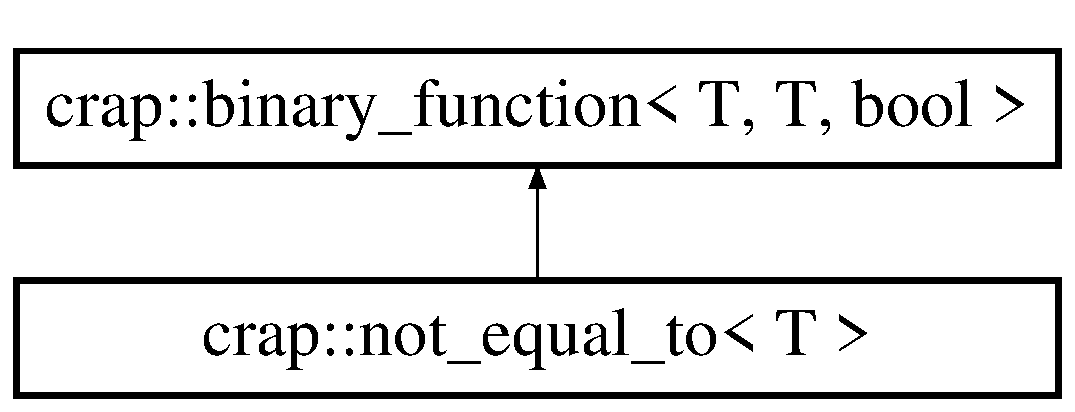
\includegraphics[height=2.000000cm]{structcrap_1_1not__equal__to}
\end{center}
\end{figure}
\subsection*{Public Member Functions}
\begin{DoxyCompactItemize}
\item 
bool \hyperlink{structcrap_1_1not__equal__to_a78f192be774943891bbe2bf725108bd7}{operator()} (const T \&x, const T \&y) const 
\end{DoxyCompactItemize}
\subsection*{Additional Inherited Members}


\subsection{Detailed Description}
\subsubsection*{template$<$class T$>$struct crap\-::not\-\_\-equal\-\_\-to$<$ T $>$}

check if first argument is not equal to second 

\subsection{Member Function Documentation}
\hypertarget{structcrap_1_1not__equal__to_a78f192be774943891bbe2bf725108bd7}{\index{crap\-::not\-\_\-equal\-\_\-to@{crap\-::not\-\_\-equal\-\_\-to}!operator()@{operator()}}
\index{operator()@{operator()}!crap::not_equal_to@{crap\-::not\-\_\-equal\-\_\-to}}
\subsubsection[{operator()}]{\setlength{\rightskip}{0pt plus 5cm}template$<$class T $>$ bool {\bf crap\-::not\-\_\-equal\-\_\-to}$<$ T $>$\-::operator() (
\begin{DoxyParamCaption}
\item[{const T \&}]{x, }
\item[{const T \&}]{y}
\end{DoxyParamCaption}
) const\hspace{0.3cm}{\ttfamily [inline]}}}\label{structcrap_1_1not__equal__to_a78f192be774943891bbe2bf725108bd7}


The documentation for this struct was generated from the following file\-:\begin{DoxyCompactItemize}
\item 
/mnt/windows/data/\-Programmierung/\-C\-R\-A\-P/src/crap/control/\hyperlink{compare_8h}{compare.\-h}\end{DoxyCompactItemize}

\hypertarget{structcrap_1_1pair}{\section{crap\-:\-:pair$<$ T1, T2 $>$ Struct Template Reference}
\label{structcrap_1_1pair}\index{crap\-::pair$<$ T1, T2 $>$@{crap\-::pair$<$ T1, T2 $>$}}
}


{\ttfamily \#include $<$pair.\-h$>$}

\subsection*{Public Types}
\begin{DoxyCompactItemize}
\item 
typedef T1 \hyperlink{structcrap_1_1pair_a3e7b8960fdb3e682b91135d1ddec2833}{first\-\_\-type}
\item 
typedef T2 \hyperlink{structcrap_1_1pair_a79e49172c1947b06e27178b7cc3f0f06}{second\-\_\-type}
\end{DoxyCompactItemize}
\subsection*{Public Member Functions}
\begin{DoxyCompactItemize}
\item 
\hyperlink{structcrap_1_1pair_aa99c7b2384e4eef00f3fefe03f3086a0}{pair} (void)
\item 
\hyperlink{structcrap_1_1pair_a5af0c0ddbf79f29dc2737a81805c2d3a}{pair} (const T1 \&x, const T2 \&y)
\item 
{\footnotesize template$<$class U , class V $>$ }\\\hyperlink{structcrap_1_1pair_a9b9de163d05aa9d2cc29945275471968}{pair} (const \hyperlink{structcrap_1_1pair}{pair}$<$ U, V $>$ \&p)
\end{DoxyCompactItemize}
\subsection*{Public Attributes}
\begin{DoxyCompactItemize}
\item 
T1 \hyperlink{structcrap_1_1pair_a1c7b7e7d1bdade135233bb71457c05b3}{first}
\item 
T2 \hyperlink{structcrap_1_1pair_ac2b9b46da996e52e23b4ecbd843a79c8}{second}
\end{DoxyCompactItemize}


\subsection{Member Typedef Documentation}
\hypertarget{structcrap_1_1pair_a3e7b8960fdb3e682b91135d1ddec2833}{\index{crap\-::pair@{crap\-::pair}!first\-\_\-type@{first\-\_\-type}}
\index{first\-\_\-type@{first\-\_\-type}!crap::pair@{crap\-::pair}}
\subsubsection[{first\-\_\-type}]{\setlength{\rightskip}{0pt plus 5cm}template$<$class T1, class T2$>$ typedef T1 {\bf crap\-::pair}$<$ T1, T2 $>$\-::{\bf first\-\_\-type}}}\label{structcrap_1_1pair_a3e7b8960fdb3e682b91135d1ddec2833}
\hypertarget{structcrap_1_1pair_a79e49172c1947b06e27178b7cc3f0f06}{\index{crap\-::pair@{crap\-::pair}!second\-\_\-type@{second\-\_\-type}}
\index{second\-\_\-type@{second\-\_\-type}!crap::pair@{crap\-::pair}}
\subsubsection[{second\-\_\-type}]{\setlength{\rightskip}{0pt plus 5cm}template$<$class T1, class T2$>$ typedef T2 {\bf crap\-::pair}$<$ T1, T2 $>$\-::{\bf second\-\_\-type}}}\label{structcrap_1_1pair_a79e49172c1947b06e27178b7cc3f0f06}


\subsection{Constructor \& Destructor Documentation}
\hypertarget{structcrap_1_1pair_aa99c7b2384e4eef00f3fefe03f3086a0}{\index{crap\-::pair@{crap\-::pair}!pair@{pair}}
\index{pair@{pair}!crap::pair@{crap\-::pair}}
\subsubsection[{pair}]{\setlength{\rightskip}{0pt plus 5cm}template$<$class T1, class T2$>$ {\bf crap\-::pair}$<$ T1, T2 $>$\-::{\bf pair} (
\begin{DoxyParamCaption}
\item[{void}]{}
\end{DoxyParamCaption}
)\hspace{0.3cm}{\ttfamily [inline]}}}\label{structcrap_1_1pair_aa99c7b2384e4eef00f3fefe03f3086a0}
\hypertarget{structcrap_1_1pair_a5af0c0ddbf79f29dc2737a81805c2d3a}{\index{crap\-::pair@{crap\-::pair}!pair@{pair}}
\index{pair@{pair}!crap::pair@{crap\-::pair}}
\subsubsection[{pair}]{\setlength{\rightskip}{0pt plus 5cm}template$<$class T1, class T2$>$ {\bf crap\-::pair}$<$ T1, T2 $>$\-::{\bf pair} (
\begin{DoxyParamCaption}
\item[{const T1 \&}]{x, }
\item[{const T2 \&}]{y}
\end{DoxyParamCaption}
)\hspace{0.3cm}{\ttfamily [inline]}}}\label{structcrap_1_1pair_a5af0c0ddbf79f29dc2737a81805c2d3a}
\hypertarget{structcrap_1_1pair_a9b9de163d05aa9d2cc29945275471968}{\index{crap\-::pair@{crap\-::pair}!pair@{pair}}
\index{pair@{pair}!crap::pair@{crap\-::pair}}
\subsubsection[{pair}]{\setlength{\rightskip}{0pt plus 5cm}template$<$class T1, class T2$>$ template$<$class U , class V $>$ {\bf crap\-::pair}$<$ T1, T2 $>$\-::{\bf pair} (
\begin{DoxyParamCaption}
\item[{const {\bf pair}$<$ U, V $>$ \&}]{p}
\end{DoxyParamCaption}
)\hspace{0.3cm}{\ttfamily [inline]}}}\label{structcrap_1_1pair_a9b9de163d05aa9d2cc29945275471968}


\subsection{Member Data Documentation}
\hypertarget{structcrap_1_1pair_a1c7b7e7d1bdade135233bb71457c05b3}{\index{crap\-::pair@{crap\-::pair}!first@{first}}
\index{first@{first}!crap::pair@{crap\-::pair}}
\subsubsection[{first}]{\setlength{\rightskip}{0pt plus 5cm}template$<$class T1, class T2$>$ T1 {\bf crap\-::pair}$<$ T1, T2 $>$\-::first}}\label{structcrap_1_1pair_a1c7b7e7d1bdade135233bb71457c05b3}
\hypertarget{structcrap_1_1pair_ac2b9b46da996e52e23b4ecbd843a79c8}{\index{crap\-::pair@{crap\-::pair}!second@{second}}
\index{second@{second}!crap::pair@{crap\-::pair}}
\subsubsection[{second}]{\setlength{\rightskip}{0pt plus 5cm}template$<$class T1, class T2$>$ T2 {\bf crap\-::pair}$<$ T1, T2 $>$\-::second}}\label{structcrap_1_1pair_ac2b9b46da996e52e23b4ecbd843a79c8}


The documentation for this struct was generated from the following file\-:\begin{DoxyCompactItemize}
\item 
/mnt/windows/data/\-Programmierung/\-C\-R\-A\-P/src/crap/container/\hyperlink{pair_8h}{pair.\-h}\end{DoxyCompactItemize}

\hypertarget{classcrap_1_1queue}{\section{crap\-:\-:queue$<$ T, Allocator $>$ Class Template Reference}
\label{classcrap_1_1queue}\index{crap\-::queue$<$ T, Allocator $>$@{crap\-::queue$<$ T, Allocator $>$}}
}


{\ttfamily \#include $<$queue.\-h$>$}

Inheritance diagram for crap\-:\-:queue$<$ T, Allocator $>$\-:\begin{figure}[H]
\begin{center}
\leavevmode
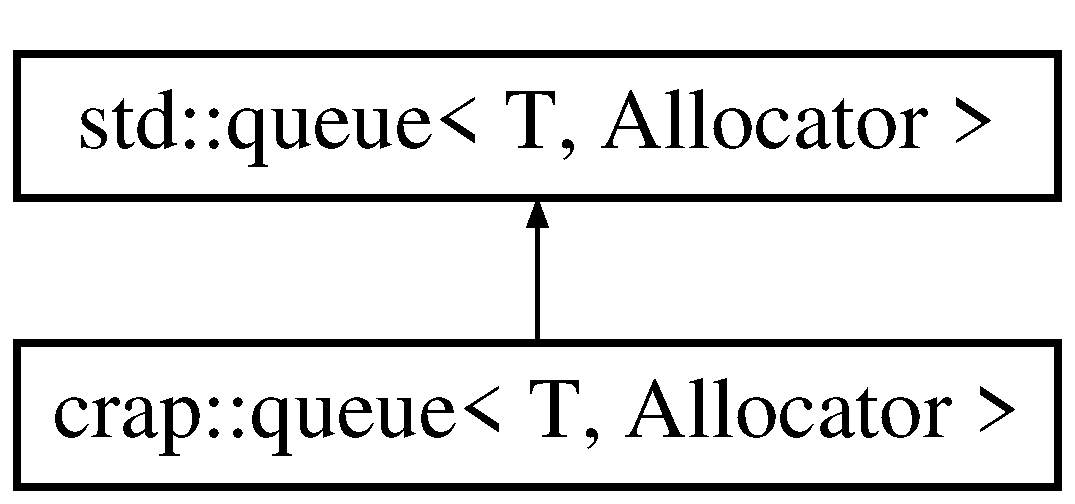
\includegraphics[height=2.000000cm]{classcrap_1_1queue}
\end{center}
\end{figure}


The documentation for this class was generated from the following file\-:\begin{DoxyCompactItemize}
\item 
/mnt/windows/data/\-Programmierung/\-C\-R\-A\-P/src/crap/container/\hyperlink{queue_8h}{queue.\-h}\end{DoxyCompactItemize}

\hypertarget{structcrap_1_1allocator__malloc_1_1rebind}{\section{crap\-:\-:allocator\-\_\-malloc$<$ T $>$\-:\-:rebind$<$ U $>$ Struct Template Reference}
\label{structcrap_1_1allocator__malloc_1_1rebind}\index{crap\-::allocator\-\_\-malloc$<$ T $>$\-::rebind$<$ U $>$@{crap\-::allocator\-\_\-malloc$<$ T $>$\-::rebind$<$ U $>$}}
}


{\ttfamily \#include $<$allocatormalloc.\-h$>$}

\subsection*{Public Types}
\begin{DoxyCompactItemize}
\item 
typedef \hyperlink{classcrap_1_1allocator__malloc}{allocator\-\_\-malloc}$<$ U $>$ \hyperlink{structcrap_1_1allocator__malloc_1_1rebind_a550f8ed979b8144b7af5aaef5949af1e}{other}
\end{DoxyCompactItemize}


\subsection{Member Typedef Documentation}
\hypertarget{structcrap_1_1allocator__malloc_1_1rebind_a550f8ed979b8144b7af5aaef5949af1e}{\index{crap\-::allocator\-\_\-malloc\-::rebind@{crap\-::allocator\-\_\-malloc\-::rebind}!other@{other}}
\index{other@{other}!crap::allocator_malloc::rebind@{crap\-::allocator\-\_\-malloc\-::rebind}}
\subsubsection[{other}]{\setlength{\rightskip}{0pt plus 5cm}template$<$typename T $>$ template$<$typename U $>$ typedef {\bf allocator\-\_\-malloc}$<$U$>$ {\bf crap\-::allocator\-\_\-malloc}$<$ T $>$\-::{\bf rebind}$<$ U $>$\-::{\bf other}}}\label{structcrap_1_1allocator__malloc_1_1rebind_a550f8ed979b8144b7af5aaef5949af1e}


The documentation for this struct was generated from the following file\-:\begin{DoxyCompactItemize}
\item 
/mnt/windows/data/\-Programmierung/\-C\-R\-A\-P/src/crap/memory/\hyperlink{allocatormalloc_8h}{allocatormalloc.\-h}\end{DoxyCompactItemize}

\hypertarget{structcrap_1_1allocator__default_1_1rebind}{\section{crap\-:\-:allocator\-\_\-default$<$ T $>$\-:\-:rebind$<$ U $>$ Struct Template Reference}
\label{structcrap_1_1allocator__default_1_1rebind}\index{crap\-::allocator\-\_\-default$<$ T $>$\-::rebind$<$ U $>$@{crap\-::allocator\-\_\-default$<$ T $>$\-::rebind$<$ U $>$}}
}


{\ttfamily \#include $<$allocatordefault.\-h$>$}

\subsection*{Public Types}
\begin{DoxyCompactItemize}
\item 
typedef \hyperlink{classcrap_1_1allocator__default}{allocator\-\_\-default}$<$ U $>$ \hyperlink{structcrap_1_1allocator__default_1_1rebind_ae93e48c1c10de1157ac200d48d92edf9}{other}
\end{DoxyCompactItemize}


\subsection{Member Typedef Documentation}
\hypertarget{structcrap_1_1allocator__default_1_1rebind_ae93e48c1c10de1157ac200d48d92edf9}{\index{crap\-::allocator\-\_\-default\-::rebind@{crap\-::allocator\-\_\-default\-::rebind}!other@{other}}
\index{other@{other}!crap::allocator_default::rebind@{crap\-::allocator\-\_\-default\-::rebind}}
\subsubsection[{other}]{\setlength{\rightskip}{0pt plus 5cm}template$<$typename T $>$ template$<$typename U $>$ typedef {\bf allocator\-\_\-default}$<$U$>$ {\bf crap\-::allocator\-\_\-default}$<$ T $>$\-::{\bf rebind}$<$ U $>$\-::{\bf other}}}\label{structcrap_1_1allocator__default_1_1rebind_ae93e48c1c10de1157ac200d48d92edf9}


The documentation for this struct was generated from the following file\-:\begin{DoxyCompactItemize}
\item 
/mnt/windows/data/\-Programmierung/\-C\-R\-A\-P/src/crap/memory/\hyperlink{allocatordefault_8h}{allocatordefault.\-h}\end{DoxyCompactItemize}

\hypertarget{classcrap_1_1runnable}{\section{crap\-:\-:runnable Class Reference}
\label{classcrap_1_1runnable}\index{crap\-::runnable@{crap\-::runnable}}
}


{\ttfamily \#include $<$runnable.\-h$>$}

\subsection*{Public Member Functions}
\begin{DoxyCompactItemize}
\item 
\hyperlink{classcrap_1_1runnable_aa748d88165fe5fa866f69352f702ed79}{runnable} (const \hyperlink{namespacecrap_a502636a1c5819e8500d07deed797ef9f}{crap\-::string64} \&\hyperlink{classcrap_1_1runnable_ab1b24cbdd09024d5a10de5d338d292fe}{name}, bool \hyperlink{classcrap_1_1runnable_a150f0d8ecb5e271e14f72fd7df2e6b0a}{delete\-\_\-on\-\_\-finish}=true)
\item 
virtual \hyperlink{classcrap_1_1runnable_a8c3b48f71f00561fe087d0ab73176490}{$\sim$runnable} ()
\item 
void $\ast$ \hyperlink{classcrap_1_1runnable_ab0d8babed68ae30351db77163b1a69e1}{start} ()
\item 
bool \hyperlink{classcrap_1_1runnable_a115719bfdaa041cb18aca0807c04a6e4}{is\-\_\-running} () const 
\item 
bool \hyperlink{classcrap_1_1runnable_a150f0d8ecb5e271e14f72fd7df2e6b0a}{delete\-\_\-on\-\_\-finish} () const 
\item 
void \hyperlink{classcrap_1_1runnable_a4a7e25ab93880d3478571a954583f016}{stop\-\_\-runnable} ()
\item 
const \hyperlink{namespacecrap_a502636a1c5819e8500d07deed797ef9f}{string64} \& \hyperlink{classcrap_1_1runnable_ab1b24cbdd09024d5a10de5d338d292fe}{name} () const 
\end{DoxyCompactItemize}
\subsection*{Protected Member Functions}
\begin{DoxyCompactItemize}
\item 
virtual void $\ast$ \hyperlink{classcrap_1_1runnable_a1736f4fc00a0d3cae71bcebdaba17658}{run} ()=0
\end{DoxyCompactItemize}
\subsection*{Protected Attributes}
\begin{DoxyCompactItemize}
\item 
bool \hyperlink{classcrap_1_1runnable_a76a8509c0a8796aa7ad0e76411947c6c}{\-\_\-is\-\_\-running}
\item 
bool \hyperlink{classcrap_1_1runnable_aa6813537f482fd8583530d7ffc807782}{\-\_\-stop\-\_\-runnable}
\item 
\hyperlink{namespacecrap_a502636a1c5819e8500d07deed797ef9f}{string64} \hyperlink{classcrap_1_1runnable_a9ad58339e7c36f7cca04c5d77950cf2d}{\-\_\-name}
\item 
bool \hyperlink{classcrap_1_1runnable_a2c7e4e875ce03711e46c996696df9be4}{\-\_\-delete\-\_\-on\-\_\-finish}
\end{DoxyCompactItemize}
\subsection*{Friends}
\begin{DoxyCompactItemize}
\item 
class \hyperlink{classcrap_1_1runnable_adb314a48b19f4325e5e69e8a60091fce}{thread}
\end{DoxyCompactItemize}


\subsection{Constructor \& Destructor Documentation}
\hypertarget{classcrap_1_1runnable_aa748d88165fe5fa866f69352f702ed79}{\index{crap\-::runnable@{crap\-::runnable}!runnable@{runnable}}
\index{runnable@{runnable}!crap::runnable@{crap\-::runnable}}
\subsubsection[{runnable}]{\setlength{\rightskip}{0pt plus 5cm}crap\-::runnable\-::runnable (
\begin{DoxyParamCaption}
\item[{const {\bf crap\-::string64} \&}]{name, }
\item[{bool}]{delete\-\_\-on\-\_\-finish = {\ttfamily true}}
\end{DoxyParamCaption}
)}}\label{classcrap_1_1runnable_aa748d88165fe5fa866f69352f702ed79}
\hypertarget{classcrap_1_1runnable_a8c3b48f71f00561fe087d0ab73176490}{\index{crap\-::runnable@{crap\-::runnable}!$\sim$runnable@{$\sim$runnable}}
\index{$\sim$runnable@{$\sim$runnable}!crap::runnable@{crap\-::runnable}}
\subsubsection[{$\sim$runnable}]{\setlength{\rightskip}{0pt plus 5cm}crap\-::runnable\-::$\sim$runnable (
\begin{DoxyParamCaption}
\item[{void}]{}
\end{DoxyParamCaption}
)\hspace{0.3cm}{\ttfamily [virtual]}}}\label{classcrap_1_1runnable_a8c3b48f71f00561fe087d0ab73176490}


\subsection{Member Function Documentation}
\hypertarget{classcrap_1_1runnable_a150f0d8ecb5e271e14f72fd7df2e6b0a}{\index{crap\-::runnable@{crap\-::runnable}!delete\-\_\-on\-\_\-finish@{delete\-\_\-on\-\_\-finish}}
\index{delete\-\_\-on\-\_\-finish@{delete\-\_\-on\-\_\-finish}!crap::runnable@{crap\-::runnable}}
\subsubsection[{delete\-\_\-on\-\_\-finish}]{\setlength{\rightskip}{0pt plus 5cm}bool crap\-::runnable\-::delete\-\_\-on\-\_\-finish (
\begin{DoxyParamCaption}
\item[{void}]{}
\end{DoxyParamCaption}
) const}}\label{classcrap_1_1runnable_a150f0d8ecb5e271e14f72fd7df2e6b0a}
\hypertarget{classcrap_1_1runnable_a115719bfdaa041cb18aca0807c04a6e4}{\index{crap\-::runnable@{crap\-::runnable}!is\-\_\-running@{is\-\_\-running}}
\index{is\-\_\-running@{is\-\_\-running}!crap::runnable@{crap\-::runnable}}
\subsubsection[{is\-\_\-running}]{\setlength{\rightskip}{0pt plus 5cm}bool crap\-::runnable\-::is\-\_\-running (
\begin{DoxyParamCaption}
\item[{void}]{}
\end{DoxyParamCaption}
) const}}\label{classcrap_1_1runnable_a115719bfdaa041cb18aca0807c04a6e4}
\hypertarget{classcrap_1_1runnable_ab1b24cbdd09024d5a10de5d338d292fe}{\index{crap\-::runnable@{crap\-::runnable}!name@{name}}
\index{name@{name}!crap::runnable@{crap\-::runnable}}
\subsubsection[{name}]{\setlength{\rightskip}{0pt plus 5cm}const {\bf crap\-::string64} \& crap\-::runnable\-::name (
\begin{DoxyParamCaption}
\item[{void}]{}
\end{DoxyParamCaption}
) const}}\label{classcrap_1_1runnable_ab1b24cbdd09024d5a10de5d338d292fe}
\hypertarget{classcrap_1_1runnable_a1736f4fc00a0d3cae71bcebdaba17658}{\index{crap\-::runnable@{crap\-::runnable}!run@{run}}
\index{run@{run}!crap::runnable@{crap\-::runnable}}
\subsubsection[{run}]{\setlength{\rightskip}{0pt plus 5cm}virtual void$\ast$ crap\-::runnable\-::run (
\begin{DoxyParamCaption}
{}
\end{DoxyParamCaption}
)\hspace{0.3cm}{\ttfamily [protected]}, {\ttfamily [pure virtual]}}}\label{classcrap_1_1runnable_a1736f4fc00a0d3cae71bcebdaba17658}
\hypertarget{classcrap_1_1runnable_ab0d8babed68ae30351db77163b1a69e1}{\index{crap\-::runnable@{crap\-::runnable}!start@{start}}
\index{start@{start}!crap::runnable@{crap\-::runnable}}
\subsubsection[{start}]{\setlength{\rightskip}{0pt plus 5cm}void $\ast$ crap\-::runnable\-::start (
\begin{DoxyParamCaption}
\item[{void}]{}
\end{DoxyParamCaption}
)}}\label{classcrap_1_1runnable_ab0d8babed68ae30351db77163b1a69e1}
\hypertarget{classcrap_1_1runnable_a4a7e25ab93880d3478571a954583f016}{\index{crap\-::runnable@{crap\-::runnable}!stop\-\_\-runnable@{stop\-\_\-runnable}}
\index{stop\-\_\-runnable@{stop\-\_\-runnable}!crap::runnable@{crap\-::runnable}}
\subsubsection[{stop\-\_\-runnable}]{\setlength{\rightskip}{0pt plus 5cm}void crap\-::runnable\-::stop\-\_\-runnable (
\begin{DoxyParamCaption}
\item[{void}]{}
\end{DoxyParamCaption}
)}}\label{classcrap_1_1runnable_a4a7e25ab93880d3478571a954583f016}


\subsection{Friends And Related Function Documentation}
\hypertarget{classcrap_1_1runnable_adb314a48b19f4325e5e69e8a60091fce}{\index{crap\-::runnable@{crap\-::runnable}!thread@{thread}}
\index{thread@{thread}!crap::runnable@{crap\-::runnable}}
\subsubsection[{thread}]{\setlength{\rightskip}{0pt plus 5cm}friend class {\bf thread}\hspace{0.3cm}{\ttfamily [friend]}}}\label{classcrap_1_1runnable_adb314a48b19f4325e5e69e8a60091fce}


\subsection{Member Data Documentation}
\hypertarget{classcrap_1_1runnable_a2c7e4e875ce03711e46c996696df9be4}{\index{crap\-::runnable@{crap\-::runnable}!\-\_\-delete\-\_\-on\-\_\-finish@{\-\_\-delete\-\_\-on\-\_\-finish}}
\index{\-\_\-delete\-\_\-on\-\_\-finish@{\-\_\-delete\-\_\-on\-\_\-finish}!crap::runnable@{crap\-::runnable}}
\subsubsection[{\-\_\-delete\-\_\-on\-\_\-finish}]{\setlength{\rightskip}{0pt plus 5cm}bool crap\-::runnable\-::\-\_\-delete\-\_\-on\-\_\-finish\hspace{0.3cm}{\ttfamily [protected]}}}\label{classcrap_1_1runnable_a2c7e4e875ce03711e46c996696df9be4}
\hypertarget{classcrap_1_1runnable_a76a8509c0a8796aa7ad0e76411947c6c}{\index{crap\-::runnable@{crap\-::runnable}!\-\_\-is\-\_\-running@{\-\_\-is\-\_\-running}}
\index{\-\_\-is\-\_\-running@{\-\_\-is\-\_\-running}!crap::runnable@{crap\-::runnable}}
\subsubsection[{\-\_\-is\-\_\-running}]{\setlength{\rightskip}{0pt plus 5cm}bool crap\-::runnable\-::\-\_\-is\-\_\-running\hspace{0.3cm}{\ttfamily [protected]}}}\label{classcrap_1_1runnable_a76a8509c0a8796aa7ad0e76411947c6c}
\hypertarget{classcrap_1_1runnable_a9ad58339e7c36f7cca04c5d77950cf2d}{\index{crap\-::runnable@{crap\-::runnable}!\-\_\-name@{\-\_\-name}}
\index{\-\_\-name@{\-\_\-name}!crap::runnable@{crap\-::runnable}}
\subsubsection[{\-\_\-name}]{\setlength{\rightskip}{0pt plus 5cm}{\bf string64} crap\-::runnable\-::\-\_\-name\hspace{0.3cm}{\ttfamily [protected]}}}\label{classcrap_1_1runnable_a9ad58339e7c36f7cca04c5d77950cf2d}
\hypertarget{classcrap_1_1runnable_aa6813537f482fd8583530d7ffc807782}{\index{crap\-::runnable@{crap\-::runnable}!\-\_\-stop\-\_\-runnable@{\-\_\-stop\-\_\-runnable}}
\index{\-\_\-stop\-\_\-runnable@{\-\_\-stop\-\_\-runnable}!crap::runnable@{crap\-::runnable}}
\subsubsection[{\-\_\-stop\-\_\-runnable}]{\setlength{\rightskip}{0pt plus 5cm}bool crap\-::runnable\-::\-\_\-stop\-\_\-runnable\hspace{0.3cm}{\ttfamily [protected]}}}\label{classcrap_1_1runnable_aa6813537f482fd8583530d7ffc807782}


The documentation for this class was generated from the following files\-:\begin{DoxyCompactItemize}
\item 
/mnt/windows/data/\-Programmierung/\-C\-R\-A\-P/src/crap/threading/\hyperlink{runnable_8h}{runnable.\-h}\item 
/mnt/windows/data/\-Programmierung/\-C\-R\-A\-P/src/crap/threading/\hyperlink{runnable_8cpp}{runnable.\-cpp}\end{DoxyCompactItemize}

\hypertarget{classcrap_1_1scope__lock}{\section{crap\-:\-:scope\-\_\-lock Class Reference}
\label{classcrap_1_1scope__lock}\index{crap\-::scope\-\_\-lock@{crap\-::scope\-\_\-lock}}
}


{\ttfamily \#include $<$scopelock.\-h$>$}

\subsection*{Public Member Functions}
\begin{DoxyCompactItemize}
\item 
\hyperlink{classcrap_1_1scope__lock_a4062ccee292ae1facbc3c09611168429}{scope\-\_\-lock} (\hyperlink{classcrap_1_1mutex}{mutex} $\ast$\hyperlink{classcrap_1_1mutex}{mutex})
\item 
\hyperlink{classcrap_1_1scope__lock_a96f02021dff94c467dc39762831415cb}{scope\-\_\-lock} (\hyperlink{classcrap_1_1semaphore}{semaphore} $\ast$\hyperlink{classcrap_1_1semaphore}{semaphore})
\item 
\hyperlink{classcrap_1_1scope__lock_a3bd9a34cdd41724e5ee7a29c0dcbbdaa}{$\sim$scope\-\_\-lock} (void)
\end{DoxyCompactItemize}


\subsection{Constructor \& Destructor Documentation}
\hypertarget{classcrap_1_1scope__lock_a4062ccee292ae1facbc3c09611168429}{\index{crap\-::scope\-\_\-lock@{crap\-::scope\-\_\-lock}!scope\-\_\-lock@{scope\-\_\-lock}}
\index{scope\-\_\-lock@{scope\-\_\-lock}!crap::scope_lock@{crap\-::scope\-\_\-lock}}
\subsubsection[{scope\-\_\-lock}]{\setlength{\rightskip}{0pt plus 5cm}crap\-::scope\-\_\-lock\-::scope\-\_\-lock (
\begin{DoxyParamCaption}
\item[{{\bf mutex} $\ast$}]{mutex}
\end{DoxyParamCaption}
)}}\label{classcrap_1_1scope__lock_a4062ccee292ae1facbc3c09611168429}
\hypertarget{classcrap_1_1scope__lock_a96f02021dff94c467dc39762831415cb}{\index{crap\-::scope\-\_\-lock@{crap\-::scope\-\_\-lock}!scope\-\_\-lock@{scope\-\_\-lock}}
\index{scope\-\_\-lock@{scope\-\_\-lock}!crap::scope_lock@{crap\-::scope\-\_\-lock}}
\subsubsection[{scope\-\_\-lock}]{\setlength{\rightskip}{0pt plus 5cm}crap\-::scope\-\_\-lock\-::scope\-\_\-lock (
\begin{DoxyParamCaption}
\item[{{\bf semaphore} $\ast$}]{semaphore}
\end{DoxyParamCaption}
)}}\label{classcrap_1_1scope__lock_a96f02021dff94c467dc39762831415cb}
\hypertarget{classcrap_1_1scope__lock_a3bd9a34cdd41724e5ee7a29c0dcbbdaa}{\index{crap\-::scope\-\_\-lock@{crap\-::scope\-\_\-lock}!$\sim$scope\-\_\-lock@{$\sim$scope\-\_\-lock}}
\index{$\sim$scope\-\_\-lock@{$\sim$scope\-\_\-lock}!crap::scope_lock@{crap\-::scope\-\_\-lock}}
\subsubsection[{$\sim$scope\-\_\-lock}]{\setlength{\rightskip}{0pt plus 5cm}crap\-::scope\-\_\-lock\-::$\sim$scope\-\_\-lock (
\begin{DoxyParamCaption}
\item[{void}]{}
\end{DoxyParamCaption}
)}}\label{classcrap_1_1scope__lock_a3bd9a34cdd41724e5ee7a29c0dcbbdaa}


The documentation for this class was generated from the following files\-:\begin{DoxyCompactItemize}
\item 
/mnt/windows/data/\-Programmierung/\-C\-R\-A\-P/src/crap/threading/\hyperlink{scopelock_8h}{scopelock.\-h}\item 
/mnt/windows/data/\-Programmierung/\-C\-R\-A\-P/src/crap/threading/\hyperlink{scopelock_8cpp}{scopelock.\-cpp}\end{DoxyCompactItemize}

\hypertarget{classcrap_1_1semaphore}{\section{crap\-:\-:semaphore Class Reference}
\label{classcrap_1_1semaphore}\index{crap\-::semaphore@{crap\-::semaphore}}
}


{\ttfamily \#include $<$semaphore.\-h$>$}

\subsection*{Public Member Functions}
\begin{DoxyCompactItemize}
\item 
\hyperlink{classcrap_1_1semaphore_af83b959cd6a4abf6b92466b9d05c2c62}{semaphore} (\hyperlink{types_8h_a48d6cd8e4135fb2ff7e7f2dac84089ec}{i32} init=0)
\item 
\hyperlink{classcrap_1_1semaphore_aca0dcce84aae3fe46b3a4fc5261afea8}{semaphore} (const \hyperlink{classcrap_1_1semaphore}{semaphore} \&other)
\item 
\hyperlink{classcrap_1_1semaphore_af6bcf4fa59d0c088d05648a772c7669e}{$\sim$semaphore} (void)
\item 
void \hyperlink{classcrap_1_1semaphore_a1674cbbfd5e4b0ca6c941b32507504dd}{operator=} (const \hyperlink{classcrap_1_1semaphore}{semaphore} \&other)
\item 
bool \hyperlink{classcrap_1_1semaphore_a4b7916d4d75f97869b3dc16a272737bc}{wait} (void) const 
\item 
bool \hyperlink{classcrap_1_1semaphore_ac29c0584914d3d53f8894eafb58eec57}{post} (void)
\item 
void \hyperlink{classcrap_1_1semaphore_a86e92049079d21e4938de7dd96f0633e}{reset} (\hyperlink{types_8h_a48d6cd8e4135fb2ff7e7f2dac84089ec}{i32} init=0)
\item 
\hyperlink{types_8h_a48d6cd8e4135fb2ff7e7f2dac84089ec}{i32} \hyperlink{classcrap_1_1semaphore_a04ba33907ab0591c0a409bcbe0fb87fc}{value} (void) const 
\end{DoxyCompactItemize}


\subsection{Constructor \& Destructor Documentation}
\hypertarget{classcrap_1_1semaphore_af83b959cd6a4abf6b92466b9d05c2c62}{\index{crap\-::semaphore@{crap\-::semaphore}!semaphore@{semaphore}}
\index{semaphore@{semaphore}!crap::semaphore@{crap\-::semaphore}}
\subsubsection[{semaphore}]{\setlength{\rightskip}{0pt plus 5cm}crap\-::semaphore\-::semaphore (
\begin{DoxyParamCaption}
\item[{{\bf i32}}]{init = {\ttfamily 0}}
\end{DoxyParamCaption}
)}}\label{classcrap_1_1semaphore_af83b959cd6a4abf6b92466b9d05c2c62}
\hypertarget{classcrap_1_1semaphore_aca0dcce84aae3fe46b3a4fc5261afea8}{\index{crap\-::semaphore@{crap\-::semaphore}!semaphore@{semaphore}}
\index{semaphore@{semaphore}!crap::semaphore@{crap\-::semaphore}}
\subsubsection[{semaphore}]{\setlength{\rightskip}{0pt plus 5cm}crap\-::semaphore\-::semaphore (
\begin{DoxyParamCaption}
\item[{const {\bf semaphore} \&}]{other}
\end{DoxyParamCaption}
)}}\label{classcrap_1_1semaphore_aca0dcce84aae3fe46b3a4fc5261afea8}
\hypertarget{classcrap_1_1semaphore_af6bcf4fa59d0c088d05648a772c7669e}{\index{crap\-::semaphore@{crap\-::semaphore}!$\sim$semaphore@{$\sim$semaphore}}
\index{$\sim$semaphore@{$\sim$semaphore}!crap::semaphore@{crap\-::semaphore}}
\subsubsection[{$\sim$semaphore}]{\setlength{\rightskip}{0pt plus 5cm}crap\-::semaphore\-::$\sim$semaphore (
\begin{DoxyParamCaption}
\item[{void}]{}
\end{DoxyParamCaption}
)}}\label{classcrap_1_1semaphore_af6bcf4fa59d0c088d05648a772c7669e}


\subsection{Member Function Documentation}
\hypertarget{classcrap_1_1semaphore_a1674cbbfd5e4b0ca6c941b32507504dd}{\index{crap\-::semaphore@{crap\-::semaphore}!operator=@{operator=}}
\index{operator=@{operator=}!crap::semaphore@{crap\-::semaphore}}
\subsubsection[{operator=}]{\setlength{\rightskip}{0pt plus 5cm}void crap\-::semaphore\-::operator= (
\begin{DoxyParamCaption}
\item[{const {\bf semaphore} \&}]{other}
\end{DoxyParamCaption}
)}}\label{classcrap_1_1semaphore_a1674cbbfd5e4b0ca6c941b32507504dd}
\hypertarget{classcrap_1_1semaphore_ac29c0584914d3d53f8894eafb58eec57}{\index{crap\-::semaphore@{crap\-::semaphore}!post@{post}}
\index{post@{post}!crap::semaphore@{crap\-::semaphore}}
\subsubsection[{post}]{\setlength{\rightskip}{0pt plus 5cm}bool crap\-::semaphore\-::post (
\begin{DoxyParamCaption}
\item[{void}]{}
\end{DoxyParamCaption}
)}}\label{classcrap_1_1semaphore_ac29c0584914d3d53f8894eafb58eec57}
\begin{DoxyRefDesc}{Todo}
\item[\hyperlink{todo__todo000003}{Todo}]\-: add timed\-Wait and try\-Wait, do they exist in Win api? \end{DoxyRefDesc}
\hypertarget{classcrap_1_1semaphore_a86e92049079d21e4938de7dd96f0633e}{\index{crap\-::semaphore@{crap\-::semaphore}!reset@{reset}}
\index{reset@{reset}!crap::semaphore@{crap\-::semaphore}}
\subsubsection[{reset}]{\setlength{\rightskip}{0pt plus 5cm}void crap\-::semaphore\-::reset (
\begin{DoxyParamCaption}
\item[{{\bf i32}}]{init = {\ttfamily 0}}
\end{DoxyParamCaption}
)}}\label{classcrap_1_1semaphore_a86e92049079d21e4938de7dd96f0633e}
\hypertarget{classcrap_1_1semaphore_a04ba33907ab0591c0a409bcbe0fb87fc}{\index{crap\-::semaphore@{crap\-::semaphore}!value@{value}}
\index{value@{value}!crap::semaphore@{crap\-::semaphore}}
\subsubsection[{value}]{\setlength{\rightskip}{0pt plus 5cm}{\bf i32} crap\-::semaphore\-::value (
\begin{DoxyParamCaption}
\item[{void}]{}
\end{DoxyParamCaption}
) const}}\label{classcrap_1_1semaphore_a04ba33907ab0591c0a409bcbe0fb87fc}
\hypertarget{classcrap_1_1semaphore_a4b7916d4d75f97869b3dc16a272737bc}{\index{crap\-::semaphore@{crap\-::semaphore}!wait@{wait}}
\index{wait@{wait}!crap::semaphore@{crap\-::semaphore}}
\subsubsection[{wait}]{\setlength{\rightskip}{0pt plus 5cm}bool crap\-::semaphore\-::wait (
\begin{DoxyParamCaption}
\item[{void}]{}
\end{DoxyParamCaption}
) const}}\label{classcrap_1_1semaphore_a4b7916d4d75f97869b3dc16a272737bc}


The documentation for this class was generated from the following files\-:\begin{DoxyCompactItemize}
\item 
/mnt/windows/data/\-Programmierung/\-C\-R\-A\-P/src/crap/threading/\hyperlink{semaphore_8h}{semaphore.\-h}\item 
/mnt/windows/data/\-Programmierung/\-C\-R\-A\-P/src/crap/threading/\hyperlink{semaphore_8cpp}{semaphore.\-cpp}\end{DoxyCompactItemize}

\hypertarget{classcrap_1_1stack}{\section{crap\-:\-:stack$<$ T, Allocator $>$ Class Template Reference}
\label{classcrap_1_1stack}\index{crap\-::stack$<$ T, Allocator $>$@{crap\-::stack$<$ T, Allocator $>$}}
}


{\ttfamily \#include $<$stack.\-h$>$}

Inheritance diagram for crap\-:\-:stack$<$ T, Allocator $>$\-:\begin{figure}[H]
\begin{center}
\leavevmode
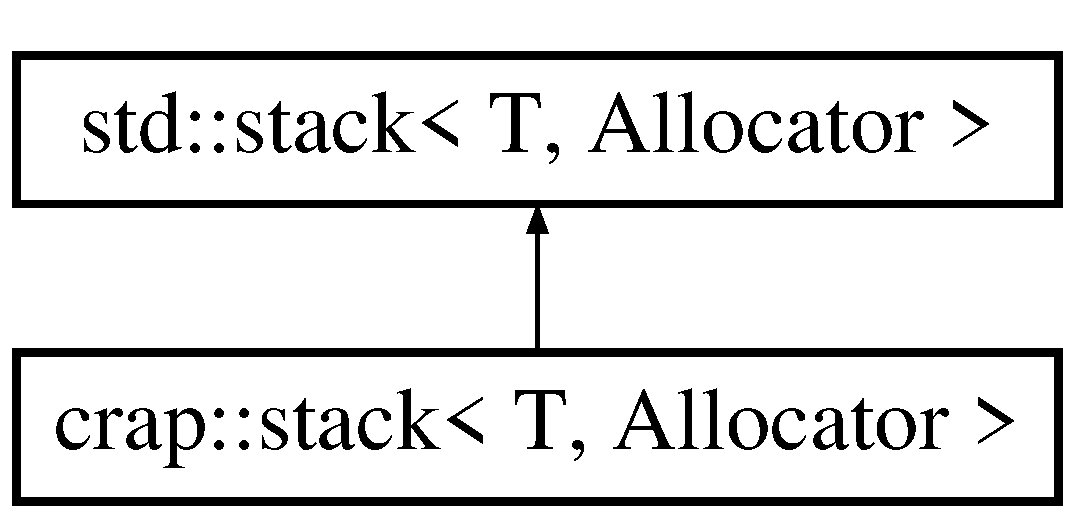
\includegraphics[height=2.000000cm]{classcrap_1_1stack}
\end{center}
\end{figure}


The documentation for this class was generated from the following file\-:\begin{DoxyCompactItemize}
\item 
/mnt/windows/data/\-Programmierung/\-C\-R\-A\-P/src/crap/container/\hyperlink{stack_8h}{stack.\-h}\end{DoxyCompactItemize}

\hypertarget{classcrap_1_1static__queue}{\section{crap\-:\-:static\-\_\-queue$<$ T, S $>$ Class Template Reference}
\label{classcrap_1_1static__queue}\index{crap\-::static\-\_\-queue$<$ T, S $>$@{crap\-::static\-\_\-queue$<$ T, S $>$}}
}


{\ttfamily \#include $<$queue.\-h$>$}

\subsection*{Public Member Functions}
\begin{DoxyCompactItemize}
\item 
\hyperlink{classcrap_1_1static__queue_a56899e95cb665eaea2fd4c7406cf31cd}{static\-\_\-queue} (void)
\begin{DoxyCompactList}\small\item\em standard constructor \end{DoxyCompactList}\item 
\hyperlink{classcrap_1_1static__queue_a2b2805029cee873b2469df1a4e99f0e5}{static\-\_\-queue} (const \hyperlink{classcrap_1_1static__queue}{static\-\_\-queue} \&other)
\begin{DoxyCompactList}\small\item\em copy constructor \end{DoxyCompactList}\item 
\hyperlink{classcrap_1_1static__queue}{static\-\_\-queue} \& \hyperlink{classcrap_1_1static__queue_a9f8cb25f63d307c44bd6feb2b1bf0d07}{operator=} (const \hyperlink{classcrap_1_1static__queue}{static\-\_\-queue} \&other)
\begin{DoxyCompactList}\small\item\em assignment operator \end{DoxyCompactList}\item 
\hyperlink{types_8h_a38c0a12279ffe0fabec44939e753c914}{size\-\_\-t32} \hyperlink{classcrap_1_1static__queue_ace84c28c7da616fd026117ecb0f489f1}{size} (void) const 
\begin{DoxyCompactList}\small\item\em returns current size \end{DoxyCompactList}\item 
\hyperlink{types_8h_a38c0a12279ffe0fabec44939e753c914}{size\-\_\-t32} \hyperlink{classcrap_1_1static__queue_abf66912fb090ccd0253416b97423bac8}{max\-\_\-size} (void) const 
\begin{DoxyCompactList}\small\item\em returns total size \end{DoxyCompactList}\item 
bool \hyperlink{classcrap_1_1static__queue_a6c20ede09aa3faca8849e97ec69b72b1}{is\-\_\-empty} (void) const 
\begin{DoxyCompactList}\small\item\em returns if queue is empty \end{DoxyCompactList}\item 
bool \hyperlink{classcrap_1_1static__queue_a4b27921670bf0540ab503043294b5c91}{is\-\_\-full} (void) const 
\begin{DoxyCompactList}\small\item\em returns if queue is full \end{DoxyCompactList}\item 
T \& \hyperlink{classcrap_1_1static__queue_ad2e008517715ad74b7d32aa3aa56f093}{front} (void)
\begin{DoxyCompactList}\small\item\em returns reference to front \end{DoxyCompactList}\item 
const T \& \hyperlink{classcrap_1_1static__queue_a74ad719cbd8afc785965e65a988e3440}{front} (void) const 
\begin{DoxyCompactList}\small\item\em returns const reference to front \end{DoxyCompactList}\item 
T \& \hyperlink{classcrap_1_1static__queue_a1ab208ae18b5188c6fe530bec2a39451}{back} (void)
\begin{DoxyCompactList}\small\item\em returns reference to back \end{DoxyCompactList}\item 
const T \& \hyperlink{classcrap_1_1static__queue_a153b42e76650c17a27673e5c4596f73b}{back} (void) const 
\begin{DoxyCompactList}\small\item\em returns const reference to back \end{DoxyCompactList}\item 
void \hyperlink{classcrap_1_1static__queue_a1a24079d7dcd7e43b45f6375bea1c8a5}{push} (const T \&object)
\begin{DoxyCompactList}\small\item\em pushes element to end of queue \end{DoxyCompactList}\item 
void \hyperlink{classcrap_1_1static__queue_aeb8ec0c469bfe24bc9fda1fed64c15cc}{pop} (void)
\begin{DoxyCompactList}\small\item\em pops element at front of queue \end{DoxyCompactList}\item 
void \hyperlink{classcrap_1_1static__queue_a5d43375db1498a62bcf08405c60172ba}{clear} (void)
\begin{DoxyCompactList}\small\item\em clear queue \end{DoxyCompactList}\end{DoxyCompactItemize}
\subsection*{Friends}
\begin{DoxyCompactItemize}
\item 
{\footnotesize template$<$typename U , u64 V$>$ }\\std\-::ostream \& \hyperlink{classcrap_1_1static__queue_a0e3f2e1085a085fd154ff8654f9ba44d}{operator$<$$<$} (std\-::ostream \&out, const \hyperlink{classcrap_1_1static__queue}{static\-\_\-queue}$<$ U, V $>$ \&other)
\begin{DoxyCompactList}\small\item\em stream operator \end{DoxyCompactList}\end{DoxyCompactItemize}


\subsection{Constructor \& Destructor Documentation}
\hypertarget{classcrap_1_1static__queue_a56899e95cb665eaea2fd4c7406cf31cd}{\index{crap\-::static\-\_\-queue@{crap\-::static\-\_\-queue}!static\-\_\-queue@{static\-\_\-queue}}
\index{static\-\_\-queue@{static\-\_\-queue}!crap::static_queue@{crap\-::static\-\_\-queue}}
\subsubsection[{static\-\_\-queue}]{\setlength{\rightskip}{0pt plus 5cm}template$<$typename T , size\-\_\-t32 S$>$ {\bf crap\-::static\-\_\-queue}$<$ T, S $>$\-::{\bf static\-\_\-queue} (
\begin{DoxyParamCaption}
\item[{void}]{}
\end{DoxyParamCaption}
)}}\label{classcrap_1_1static__queue_a56899e95cb665eaea2fd4c7406cf31cd}


standard constructor 

\hypertarget{classcrap_1_1static__queue_a2b2805029cee873b2469df1a4e99f0e5}{\index{crap\-::static\-\_\-queue@{crap\-::static\-\_\-queue}!static\-\_\-queue@{static\-\_\-queue}}
\index{static\-\_\-queue@{static\-\_\-queue}!crap::static_queue@{crap\-::static\-\_\-queue}}
\subsubsection[{static\-\_\-queue}]{\setlength{\rightskip}{0pt plus 5cm}template$<$typename T , size\-\_\-t32 S$>$ {\bf crap\-::static\-\_\-queue}$<$ T, S $>$\-::{\bf static\-\_\-queue} (
\begin{DoxyParamCaption}
\item[{const {\bf static\-\_\-queue}$<$ T, S $>$ \&}]{other}
\end{DoxyParamCaption}
)}}\label{classcrap_1_1static__queue_a2b2805029cee873b2469df1a4e99f0e5}


copy constructor 



\subsection{Member Function Documentation}
\hypertarget{classcrap_1_1static__queue_a1ab208ae18b5188c6fe530bec2a39451}{\index{crap\-::static\-\_\-queue@{crap\-::static\-\_\-queue}!back@{back}}
\index{back@{back}!crap::static_queue@{crap\-::static\-\_\-queue}}
\subsubsection[{back}]{\setlength{\rightskip}{0pt plus 5cm}template$<$typename T , size\-\_\-t32 S$>$ T \& {\bf crap\-::static\-\_\-queue}$<$ T, S $>$\-::back (
\begin{DoxyParamCaption}
\item[{void}]{}
\end{DoxyParamCaption}
)}}\label{classcrap_1_1static__queue_a1ab208ae18b5188c6fe530bec2a39451}


returns reference to back 

\hypertarget{classcrap_1_1static__queue_a153b42e76650c17a27673e5c4596f73b}{\index{crap\-::static\-\_\-queue@{crap\-::static\-\_\-queue}!back@{back}}
\index{back@{back}!crap::static_queue@{crap\-::static\-\_\-queue}}
\subsubsection[{back}]{\setlength{\rightskip}{0pt plus 5cm}template$<$typename T , size\-\_\-t32 S$>$ const T \& {\bf crap\-::static\-\_\-queue}$<$ T, S $>$\-::back (
\begin{DoxyParamCaption}
\item[{void}]{}
\end{DoxyParamCaption}
) const}}\label{classcrap_1_1static__queue_a153b42e76650c17a27673e5c4596f73b}


returns const reference to back 

\hypertarget{classcrap_1_1static__queue_a5d43375db1498a62bcf08405c60172ba}{\index{crap\-::static\-\_\-queue@{crap\-::static\-\_\-queue}!clear@{clear}}
\index{clear@{clear}!crap::static_queue@{crap\-::static\-\_\-queue}}
\subsubsection[{clear}]{\setlength{\rightskip}{0pt plus 5cm}template$<$typename T , size\-\_\-t32 S$>$ void {\bf crap\-::static\-\_\-queue}$<$ T, S $>$\-::clear (
\begin{DoxyParamCaption}
\item[{void}]{}
\end{DoxyParamCaption}
)}}\label{classcrap_1_1static__queue_a5d43375db1498a62bcf08405c60172ba}


clear queue 

\hypertarget{classcrap_1_1static__queue_ad2e008517715ad74b7d32aa3aa56f093}{\index{crap\-::static\-\_\-queue@{crap\-::static\-\_\-queue}!front@{front}}
\index{front@{front}!crap::static_queue@{crap\-::static\-\_\-queue}}
\subsubsection[{front}]{\setlength{\rightskip}{0pt plus 5cm}template$<$typename T , size\-\_\-t32 S$>$ T \& {\bf crap\-::static\-\_\-queue}$<$ T, S $>$\-::front (
\begin{DoxyParamCaption}
\item[{void}]{}
\end{DoxyParamCaption}
)}}\label{classcrap_1_1static__queue_ad2e008517715ad74b7d32aa3aa56f093}


returns reference to front 

\hypertarget{classcrap_1_1static__queue_a74ad719cbd8afc785965e65a988e3440}{\index{crap\-::static\-\_\-queue@{crap\-::static\-\_\-queue}!front@{front}}
\index{front@{front}!crap::static_queue@{crap\-::static\-\_\-queue}}
\subsubsection[{front}]{\setlength{\rightskip}{0pt plus 5cm}template$<$typename T , size\-\_\-t32 S$>$ const T \& {\bf crap\-::static\-\_\-queue}$<$ T, S $>$\-::front (
\begin{DoxyParamCaption}
\item[{void}]{}
\end{DoxyParamCaption}
) const}}\label{classcrap_1_1static__queue_a74ad719cbd8afc785965e65a988e3440}


returns const reference to front 

\hypertarget{classcrap_1_1static__queue_a6c20ede09aa3faca8849e97ec69b72b1}{\index{crap\-::static\-\_\-queue@{crap\-::static\-\_\-queue}!is\-\_\-empty@{is\-\_\-empty}}
\index{is\-\_\-empty@{is\-\_\-empty}!crap::static_queue@{crap\-::static\-\_\-queue}}
\subsubsection[{is\-\_\-empty}]{\setlength{\rightskip}{0pt plus 5cm}template$<$typename T , size\-\_\-t32 S$>$ bool {\bf crap\-::static\-\_\-queue}$<$ T, S $>$\-::is\-\_\-empty (
\begin{DoxyParamCaption}
\item[{void}]{}
\end{DoxyParamCaption}
) const}}\label{classcrap_1_1static__queue_a6c20ede09aa3faca8849e97ec69b72b1}


returns if queue is empty 

\hypertarget{classcrap_1_1static__queue_a4b27921670bf0540ab503043294b5c91}{\index{crap\-::static\-\_\-queue@{crap\-::static\-\_\-queue}!is\-\_\-full@{is\-\_\-full}}
\index{is\-\_\-full@{is\-\_\-full}!crap::static_queue@{crap\-::static\-\_\-queue}}
\subsubsection[{is\-\_\-full}]{\setlength{\rightskip}{0pt plus 5cm}template$<$typename T , size\-\_\-t32 S$>$ bool {\bf crap\-::static\-\_\-queue}$<$ T, S $>$\-::is\-\_\-full (
\begin{DoxyParamCaption}
\item[{void}]{}
\end{DoxyParamCaption}
) const}}\label{classcrap_1_1static__queue_a4b27921670bf0540ab503043294b5c91}


returns if queue is full 

\hypertarget{classcrap_1_1static__queue_abf66912fb090ccd0253416b97423bac8}{\index{crap\-::static\-\_\-queue@{crap\-::static\-\_\-queue}!max\-\_\-size@{max\-\_\-size}}
\index{max\-\_\-size@{max\-\_\-size}!crap::static_queue@{crap\-::static\-\_\-queue}}
\subsubsection[{max\-\_\-size}]{\setlength{\rightskip}{0pt plus 5cm}template$<$typename T , size\-\_\-t32 S$>$ {\bf size\-\_\-t32} {\bf crap\-::static\-\_\-queue}$<$ T, S $>$\-::max\-\_\-size (
\begin{DoxyParamCaption}
\item[{void}]{}
\end{DoxyParamCaption}
) const}}\label{classcrap_1_1static__queue_abf66912fb090ccd0253416b97423bac8}


returns total size 

\hypertarget{classcrap_1_1static__queue_a9f8cb25f63d307c44bd6feb2b1bf0d07}{\index{crap\-::static\-\_\-queue@{crap\-::static\-\_\-queue}!operator=@{operator=}}
\index{operator=@{operator=}!crap::static_queue@{crap\-::static\-\_\-queue}}
\subsubsection[{operator=}]{\setlength{\rightskip}{0pt plus 5cm}template$<$typename T , size\-\_\-t32 S$>$ {\bf static\-\_\-queue}$<$ T, S $>$ \& {\bf crap\-::static\-\_\-queue}$<$ T, S $>$\-::operator= (
\begin{DoxyParamCaption}
\item[{const {\bf static\-\_\-queue}$<$ T, S $>$ \&}]{other}
\end{DoxyParamCaption}
)}}\label{classcrap_1_1static__queue_a9f8cb25f63d307c44bd6feb2b1bf0d07}


assignment operator 

\hypertarget{classcrap_1_1static__queue_aeb8ec0c469bfe24bc9fda1fed64c15cc}{\index{crap\-::static\-\_\-queue@{crap\-::static\-\_\-queue}!pop@{pop}}
\index{pop@{pop}!crap::static_queue@{crap\-::static\-\_\-queue}}
\subsubsection[{pop}]{\setlength{\rightskip}{0pt plus 5cm}template$<$typename T , size\-\_\-t32 S$>$ void {\bf crap\-::static\-\_\-queue}$<$ T, S $>$\-::pop (
\begin{DoxyParamCaption}
\item[{void}]{}
\end{DoxyParamCaption}
)}}\label{classcrap_1_1static__queue_aeb8ec0c469bfe24bc9fda1fed64c15cc}


pops element at front of queue 

\hypertarget{classcrap_1_1static__queue_a1a24079d7dcd7e43b45f6375bea1c8a5}{\index{crap\-::static\-\_\-queue@{crap\-::static\-\_\-queue}!push@{push}}
\index{push@{push}!crap::static_queue@{crap\-::static\-\_\-queue}}
\subsubsection[{push}]{\setlength{\rightskip}{0pt plus 5cm}template$<$typename T , size\-\_\-t32 S$>$ void {\bf crap\-::static\-\_\-queue}$<$ T, S $>$\-::push (
\begin{DoxyParamCaption}
\item[{const T \&}]{object}
\end{DoxyParamCaption}
)}}\label{classcrap_1_1static__queue_a1a24079d7dcd7e43b45f6375bea1c8a5}


pushes element to end of queue 

\hypertarget{classcrap_1_1static__queue_ace84c28c7da616fd026117ecb0f489f1}{\index{crap\-::static\-\_\-queue@{crap\-::static\-\_\-queue}!size@{size}}
\index{size@{size}!crap::static_queue@{crap\-::static\-\_\-queue}}
\subsubsection[{size}]{\setlength{\rightskip}{0pt plus 5cm}template$<$typename T , size\-\_\-t32 S$>$ {\bf size\-\_\-t32} {\bf crap\-::static\-\_\-queue}$<$ T, S $>$\-::size (
\begin{DoxyParamCaption}
\item[{void}]{}
\end{DoxyParamCaption}
) const}}\label{classcrap_1_1static__queue_ace84c28c7da616fd026117ecb0f489f1}


returns current size 



\subsection{Friends And Related Function Documentation}
\hypertarget{classcrap_1_1static__queue_a0e3f2e1085a085fd154ff8654f9ba44d}{\index{crap\-::static\-\_\-queue@{crap\-::static\-\_\-queue}!operator$<$$<$@{operator$<$$<$}}
\index{operator$<$$<$@{operator$<$$<$}!crap::static_queue@{crap\-::static\-\_\-queue}}
\subsubsection[{operator$<$$<$}]{\setlength{\rightskip}{0pt plus 5cm}template$<$typename T , size\-\_\-t32 S$>$ template$<$typename U , u64 V$>$ std\-::ostream\& operator$<$$<$ (
\begin{DoxyParamCaption}
\item[{std\-::ostream \&}]{out, }
\item[{const {\bf static\-\_\-queue}$<$ U, V $>$ \&}]{other}
\end{DoxyParamCaption}
)\hspace{0.3cm}{\ttfamily [friend]}}}\label{classcrap_1_1static__queue_a0e3f2e1085a085fd154ff8654f9ba44d}


stream operator 



The documentation for this class was generated from the following file\-:\begin{DoxyCompactItemize}
\item 
/mnt/windows/data/\-Programmierung/\-C\-R\-A\-P/src/crap/container/\hyperlink{queue_8h}{queue.\-h}\end{DoxyCompactItemize}

\hypertarget{classcrap_1_1static__stack}{\section{crap\-:\-:static\-\_\-stack$<$ T, S $>$ Class Template Reference}
\label{classcrap_1_1static__stack}\index{crap\-::static\-\_\-stack$<$ T, S $>$@{crap\-::static\-\_\-stack$<$ T, S $>$}}
}


{\ttfamily \#include $<$stack.\-h$>$}

\subsection*{Public Member Functions}
\begin{DoxyCompactItemize}
\item 
\hyperlink{classcrap_1_1static__stack_a8d15d6a53bf2358c2a2ff52e8e8e8a31}{static\-\_\-stack} (void)
\begin{DoxyCompactList}\small\item\em default constructor \end{DoxyCompactList}\item 
\hyperlink{classcrap_1_1static__stack_ab037da1dd38ecb31f43e4f865827aa71}{static\-\_\-stack} (const \hyperlink{classcrap_1_1static__stack}{static\-\_\-stack} \&other)
\begin{DoxyCompactList}\small\item\em copy constructor \end{DoxyCompactList}\item 
\hyperlink{classcrap_1_1static__stack}{static\-\_\-stack} \& \hyperlink{classcrap_1_1static__stack_a9351919bcadd21872d8ab246ecf42a19}{operator=} (const \hyperlink{classcrap_1_1static__stack}{static\-\_\-stack} \&other)
\begin{DoxyCompactList}\small\item\em assignment operator \end{DoxyCompactList}\item 
\hyperlink{types_8h_a38c0a12279ffe0fabec44939e753c914}{size\-\_\-t32} \hyperlink{classcrap_1_1static__stack_a765910dc7827be3a8187ed4c1e9f4262}{size} (void) const 
\begin{DoxyCompactList}\small\item\em returns current size of stack \end{DoxyCompactList}\item 
\hyperlink{types_8h_a38c0a12279ffe0fabec44939e753c914}{size\-\_\-t32} \hyperlink{classcrap_1_1static__stack_ac2952d1a201c89a14c23df6f47a51303}{max\-\_\-size} (void) const 
\begin{DoxyCompactList}\small\item\em returns maximum size of stack \end{DoxyCompactList}\item 
bool \hyperlink{classcrap_1_1static__stack_a50b7dac79d2a44937463cf32bfe3ba24}{is\-\_\-empty} (void) const 
\begin{DoxyCompactList}\small\item\em returns if stack is empty \end{DoxyCompactList}\item 
bool \hyperlink{classcrap_1_1static__stack_a92b967247a7a5d515d45a130f65b4d06}{is\-\_\-full} (void) const 
\begin{DoxyCompactList}\small\item\em returns if stack is full \end{DoxyCompactList}\item 
T \& \hyperlink{classcrap_1_1static__stack_acb5592dd4569da537d9b83e5f01be9a3}{top} (void)
\begin{DoxyCompactList}\small\item\em returns reference to front object \end{DoxyCompactList}\item 
const T \& \hyperlink{classcrap_1_1static__stack_a65067039b14027a4f9de84c3777408f1}{top} (void) const 
\begin{DoxyCompactList}\small\item\em returns const reference to front object \end{DoxyCompactList}\item 
void \hyperlink{classcrap_1_1static__stack_aad405e79112eda4558f5758da01bb8f3}{push} (const T \&object)
\begin{DoxyCompactList}\small\item\em push new object to top of stack \end{DoxyCompactList}\item 
void \hyperlink{classcrap_1_1static__stack_a9d0564eb1707f2e470ba2ee7b3e965ff}{pop} (void)
\begin{DoxyCompactList}\small\item\em pop top element of stack \end{DoxyCompactList}\item 
void \hyperlink{classcrap_1_1static__stack_aaa488bb2ed8979506bd4704ec1da8d37}{clear} (void)
\begin{DoxyCompactList}\small\item\em clear stack \end{DoxyCompactList}\end{DoxyCompactItemize}
\subsection*{Friends}
\begin{DoxyCompactItemize}
\item 
{\footnotesize template$<$typename U , u64 V$>$ }\\std\-::ostream \& \hyperlink{classcrap_1_1static__stack_aa9e09b8cd269462971c695b9b0a6a205}{operator$<$$<$} (std\-::ostream \&out, const \hyperlink{classcrap_1_1static__stack}{static\-\_\-stack}$<$ U, V $>$ \&other)
\begin{DoxyCompactList}\small\item\em stream operator \end{DoxyCompactList}\end{DoxyCompactItemize}


\subsection{Constructor \& Destructor Documentation}
\hypertarget{classcrap_1_1static__stack_a8d15d6a53bf2358c2a2ff52e8e8e8a31}{\index{crap\-::static\-\_\-stack@{crap\-::static\-\_\-stack}!static\-\_\-stack@{static\-\_\-stack}}
\index{static\-\_\-stack@{static\-\_\-stack}!crap::static_stack@{crap\-::static\-\_\-stack}}
\subsubsection[{static\-\_\-stack}]{\setlength{\rightskip}{0pt plus 5cm}template$<$typename T , size\-\_\-t32 S$>$ {\bf crap\-::static\-\_\-stack}$<$ T, S $>$\-::{\bf static\-\_\-stack} (
\begin{DoxyParamCaption}
\item[{void}]{}
\end{DoxyParamCaption}
)}}\label{classcrap_1_1static__stack_a8d15d6a53bf2358c2a2ff52e8e8e8a31}


default constructor 

\hypertarget{classcrap_1_1static__stack_ab037da1dd38ecb31f43e4f865827aa71}{\index{crap\-::static\-\_\-stack@{crap\-::static\-\_\-stack}!static\-\_\-stack@{static\-\_\-stack}}
\index{static\-\_\-stack@{static\-\_\-stack}!crap::static_stack@{crap\-::static\-\_\-stack}}
\subsubsection[{static\-\_\-stack}]{\setlength{\rightskip}{0pt plus 5cm}template$<$typename T , size\-\_\-t32 S$>$ {\bf crap\-::static\-\_\-stack}$<$ T, S $>$\-::{\bf static\-\_\-stack} (
\begin{DoxyParamCaption}
\item[{const {\bf static\-\_\-stack}$<$ T, S $>$ \&}]{other}
\end{DoxyParamCaption}
)}}\label{classcrap_1_1static__stack_ab037da1dd38ecb31f43e4f865827aa71}


copy constructor 



\subsection{Member Function Documentation}
\hypertarget{classcrap_1_1static__stack_aaa488bb2ed8979506bd4704ec1da8d37}{\index{crap\-::static\-\_\-stack@{crap\-::static\-\_\-stack}!clear@{clear}}
\index{clear@{clear}!crap::static_stack@{crap\-::static\-\_\-stack}}
\subsubsection[{clear}]{\setlength{\rightskip}{0pt plus 5cm}template$<$typename T , size\-\_\-t32 S$>$ void {\bf crap\-::static\-\_\-stack}$<$ T, S $>$\-::clear (
\begin{DoxyParamCaption}
\item[{void}]{}
\end{DoxyParamCaption}
)}}\label{classcrap_1_1static__stack_aaa488bb2ed8979506bd4704ec1da8d37}


clear stack 

\hypertarget{classcrap_1_1static__stack_a50b7dac79d2a44937463cf32bfe3ba24}{\index{crap\-::static\-\_\-stack@{crap\-::static\-\_\-stack}!is\-\_\-empty@{is\-\_\-empty}}
\index{is\-\_\-empty@{is\-\_\-empty}!crap::static_stack@{crap\-::static\-\_\-stack}}
\subsubsection[{is\-\_\-empty}]{\setlength{\rightskip}{0pt plus 5cm}template$<$typename T , size\-\_\-t32 S$>$ bool {\bf crap\-::static\-\_\-stack}$<$ T, S $>$\-::is\-\_\-empty (
\begin{DoxyParamCaption}
\item[{void}]{}
\end{DoxyParamCaption}
) const}}\label{classcrap_1_1static__stack_a50b7dac79d2a44937463cf32bfe3ba24}


returns if stack is empty 

\hypertarget{classcrap_1_1static__stack_a92b967247a7a5d515d45a130f65b4d06}{\index{crap\-::static\-\_\-stack@{crap\-::static\-\_\-stack}!is\-\_\-full@{is\-\_\-full}}
\index{is\-\_\-full@{is\-\_\-full}!crap::static_stack@{crap\-::static\-\_\-stack}}
\subsubsection[{is\-\_\-full}]{\setlength{\rightskip}{0pt plus 5cm}template$<$typename T , size\-\_\-t32 S$>$ bool {\bf crap\-::static\-\_\-stack}$<$ T, S $>$\-::is\-\_\-full (
\begin{DoxyParamCaption}
\item[{void}]{}
\end{DoxyParamCaption}
) const}}\label{classcrap_1_1static__stack_a92b967247a7a5d515d45a130f65b4d06}


returns if stack is full 

\hypertarget{classcrap_1_1static__stack_ac2952d1a201c89a14c23df6f47a51303}{\index{crap\-::static\-\_\-stack@{crap\-::static\-\_\-stack}!max\-\_\-size@{max\-\_\-size}}
\index{max\-\_\-size@{max\-\_\-size}!crap::static_stack@{crap\-::static\-\_\-stack}}
\subsubsection[{max\-\_\-size}]{\setlength{\rightskip}{0pt plus 5cm}template$<$typename T , size\-\_\-t32 S$>$ {\bf size\-\_\-t32} {\bf crap\-::static\-\_\-stack}$<$ T, S $>$\-::max\-\_\-size (
\begin{DoxyParamCaption}
\item[{void}]{}
\end{DoxyParamCaption}
) const}}\label{classcrap_1_1static__stack_ac2952d1a201c89a14c23df6f47a51303}


returns maximum size of stack 

\hypertarget{classcrap_1_1static__stack_a9351919bcadd21872d8ab246ecf42a19}{\index{crap\-::static\-\_\-stack@{crap\-::static\-\_\-stack}!operator=@{operator=}}
\index{operator=@{operator=}!crap::static_stack@{crap\-::static\-\_\-stack}}
\subsubsection[{operator=}]{\setlength{\rightskip}{0pt plus 5cm}template$<$typename T , size\-\_\-t32 S$>$ {\bf static\-\_\-stack}$<$ T, S $>$ \& {\bf crap\-::static\-\_\-stack}$<$ T, S $>$\-::operator= (
\begin{DoxyParamCaption}
\item[{const {\bf static\-\_\-stack}$<$ T, S $>$ \&}]{other}
\end{DoxyParamCaption}
)}}\label{classcrap_1_1static__stack_a9351919bcadd21872d8ab246ecf42a19}


assignment operator 

\hypertarget{classcrap_1_1static__stack_a9d0564eb1707f2e470ba2ee7b3e965ff}{\index{crap\-::static\-\_\-stack@{crap\-::static\-\_\-stack}!pop@{pop}}
\index{pop@{pop}!crap::static_stack@{crap\-::static\-\_\-stack}}
\subsubsection[{pop}]{\setlength{\rightskip}{0pt plus 5cm}template$<$typename T , size\-\_\-t32 S$>$ void {\bf crap\-::static\-\_\-stack}$<$ T, S $>$\-::pop (
\begin{DoxyParamCaption}
\item[{void}]{}
\end{DoxyParamCaption}
)}}\label{classcrap_1_1static__stack_a9d0564eb1707f2e470ba2ee7b3e965ff}


pop top element of stack 

\hypertarget{classcrap_1_1static__stack_aad405e79112eda4558f5758da01bb8f3}{\index{crap\-::static\-\_\-stack@{crap\-::static\-\_\-stack}!push@{push}}
\index{push@{push}!crap::static_stack@{crap\-::static\-\_\-stack}}
\subsubsection[{push}]{\setlength{\rightskip}{0pt plus 5cm}template$<$typename T , size\-\_\-t32 S$>$ void {\bf crap\-::static\-\_\-stack}$<$ T, S $>$\-::push (
\begin{DoxyParamCaption}
\item[{const T \&}]{object}
\end{DoxyParamCaption}
)}}\label{classcrap_1_1static__stack_aad405e79112eda4558f5758da01bb8f3}


push new object to top of stack 

\hypertarget{classcrap_1_1static__stack_a765910dc7827be3a8187ed4c1e9f4262}{\index{crap\-::static\-\_\-stack@{crap\-::static\-\_\-stack}!size@{size}}
\index{size@{size}!crap::static_stack@{crap\-::static\-\_\-stack}}
\subsubsection[{size}]{\setlength{\rightskip}{0pt plus 5cm}template$<$typename T , size\-\_\-t32 S$>$ {\bf size\-\_\-t32} {\bf crap\-::static\-\_\-stack}$<$ T, S $>$\-::size (
\begin{DoxyParamCaption}
\item[{void}]{}
\end{DoxyParamCaption}
) const}}\label{classcrap_1_1static__stack_a765910dc7827be3a8187ed4c1e9f4262}


returns current size of stack 

\hypertarget{classcrap_1_1static__stack_acb5592dd4569da537d9b83e5f01be9a3}{\index{crap\-::static\-\_\-stack@{crap\-::static\-\_\-stack}!top@{top}}
\index{top@{top}!crap::static_stack@{crap\-::static\-\_\-stack}}
\subsubsection[{top}]{\setlength{\rightskip}{0pt plus 5cm}template$<$typename T , size\-\_\-t32 S$>$ T \& {\bf crap\-::static\-\_\-stack}$<$ T, S $>$\-::top (
\begin{DoxyParamCaption}
\item[{void}]{}
\end{DoxyParamCaption}
)}}\label{classcrap_1_1static__stack_acb5592dd4569da537d9b83e5f01be9a3}


returns reference to front object 

\hypertarget{classcrap_1_1static__stack_a65067039b14027a4f9de84c3777408f1}{\index{crap\-::static\-\_\-stack@{crap\-::static\-\_\-stack}!top@{top}}
\index{top@{top}!crap::static_stack@{crap\-::static\-\_\-stack}}
\subsubsection[{top}]{\setlength{\rightskip}{0pt plus 5cm}template$<$typename T , size\-\_\-t32 S$>$ const T \& {\bf crap\-::static\-\_\-stack}$<$ T, S $>$\-::top (
\begin{DoxyParamCaption}
\item[{void}]{}
\end{DoxyParamCaption}
) const}}\label{classcrap_1_1static__stack_a65067039b14027a4f9de84c3777408f1}


returns const reference to front object 



\subsection{Friends And Related Function Documentation}
\hypertarget{classcrap_1_1static__stack_aa9e09b8cd269462971c695b9b0a6a205}{\index{crap\-::static\-\_\-stack@{crap\-::static\-\_\-stack}!operator$<$$<$@{operator$<$$<$}}
\index{operator$<$$<$@{operator$<$$<$}!crap::static_stack@{crap\-::static\-\_\-stack}}
\subsubsection[{operator$<$$<$}]{\setlength{\rightskip}{0pt plus 5cm}template$<$typename T , size\-\_\-t32 S$>$ template$<$typename U , u64 V$>$ std\-::ostream\& operator$<$$<$ (
\begin{DoxyParamCaption}
\item[{std\-::ostream \&}]{out, }
\item[{const {\bf static\-\_\-stack}$<$ U, V $>$ \&}]{other}
\end{DoxyParamCaption}
)\hspace{0.3cm}{\ttfamily [friend]}}}\label{classcrap_1_1static__stack_aa9e09b8cd269462971c695b9b0a6a205}


stream operator 



The documentation for this class was generated from the following file\-:\begin{DoxyCompactItemize}
\item 
/mnt/windows/data/\-Programmierung/\-C\-R\-A\-P/src/crap/container/\hyperlink{stack_8h}{stack.\-h}\end{DoxyCompactItemize}

\hypertarget{classcrap_1_1static__string}{\section{crap\-:\-:static\-\_\-string$<$ S $>$ Class Template Reference}
\label{classcrap_1_1static__string}\index{crap\-::static\-\_\-string$<$ S $>$@{crap\-::static\-\_\-string$<$ S $>$}}
}


{\ttfamily \#include $<$staticstring.\-h$>$}

\subsection*{Public Member Functions}
\begin{DoxyCompactItemize}
\item 
\hyperlink{classcrap_1_1static__string_a60906d73d636bfef77ee97f8fe057932}{static\-\_\-string} (void)
\item 
\hyperlink{classcrap_1_1static__string_ad9e5c7edf444016c85a8b7362a16815b}{static\-\_\-string} (const \hyperlink{classcrap_1_1static__string}{static\-\_\-string} \&other)
\item 
\hyperlink{classcrap_1_1static__string_ac8053cc4d317a2983ca1f4202754ed0e}{static\-\_\-string} (\hyperlink{types_8h_a5849681cb91aa8afef6996d9d9e90881}{cstring} $\ast$format,...)
\item 
\hyperlink{classcrap_1_1static__string}{static\-\_\-string} \& \hyperlink{classcrap_1_1static__string_a64b46f58329ad02ab98930ac0bd0da81}{operator=} (const \hyperlink{classcrap_1_1static__string}{static\-\_\-string} \&other)
\item 
\hyperlink{classcrap_1_1static__string}{static\-\_\-string} \& \hyperlink{classcrap_1_1static__string_a121abadd478db86946f2862e08281048}{operator=} (\hyperlink{types_8h_a5849681cb91aa8afef6996d9d9e90881}{cstring} $\ast$cstr)
\item 
\hyperlink{classcrap_1_1static__string}{static\-\_\-string} \& \hyperlink{classcrap_1_1static__string_ac1560d3ca733b576d0db85d2b95005d2}{operator+=} (const \hyperlink{classcrap_1_1static__string}{static\-\_\-string} \&other)
\item 
\hyperlink{classcrap_1_1static__string}{static\-\_\-string} \& \hyperlink{classcrap_1_1static__string_ad70525084df145ba9e9e297bb773edc4}{operator+=} (\hyperlink{types_8h_a5849681cb91aa8afef6996d9d9e90881}{cstring} $\ast$cstr)
\item 
bool \hyperlink{classcrap_1_1static__string_a6ce1a4474db9a8f130a3a0cd9d4e557e}{operator==} (const \hyperlink{classcrap_1_1static__string}{static\-\_\-string} \&other) const 
\item 
bool \hyperlink{classcrap_1_1static__string_adcc51a627f454f0eeb92b454bc2fca4d}{operator==} (\hyperlink{types_8h_a5849681cb91aa8afef6996d9d9e90881}{cstring} $\ast$cstr) const 
\item 
bool \hyperlink{classcrap_1_1static__string_a9d345213c368dae1cd2ed4baa67c8e9d}{operator!=} (const \hyperlink{classcrap_1_1static__string}{static\-\_\-string} \&other) const 
\item 
bool \hyperlink{classcrap_1_1static__string_a7c03171e5e4b78cb06d2f8b2fe5e3c97}{operator!=} (\hyperlink{types_8h_a5849681cb91aa8afef6996d9d9e90881}{cstring} $\ast$cstr) const 
\item 
\hyperlink{types_8h_aa1ba8aac9fcd831012308297336ac74b}{c8} \& \hyperlink{classcrap_1_1static__string_aa3b0e1dec3e338c823915ca243cc5598}{operator\mbox{[}$\,$\mbox{]}} (\hyperlink{types_8h_a38c0a12279ffe0fabec44939e753c914}{size\-\_\-t32} index)
\item 
const \hyperlink{types_8h_aa1ba8aac9fcd831012308297336ac74b}{c8} \& \hyperlink{classcrap_1_1static__string_a30c88a298dcc6d8bcd72264949a9da1e}{operator\mbox{[}$\,$\mbox{]}} (\hyperlink{types_8h_a38c0a12279ffe0fabec44939e753c914}{size\-\_\-t32} index) const 
\item 
void \hyperlink{classcrap_1_1static__string_a9bc69ea62fb9cbcafec6a12a383de24b}{concat} (const \hyperlink{classcrap_1_1static__string}{static\-\_\-string} \&other)
\item 
void \hyperlink{classcrap_1_1static__string_a242b130d6a27e8ca19470efbb684635d}{concat} (\hyperlink{types_8h_a5849681cb91aa8afef6996d9d9e90881}{cstring} $\ast$cstr)
\item 
bool \hyperlink{classcrap_1_1static__string_ae9177cdc25cd6c8c9a4b347ee688d3e3}{compare} (const \hyperlink{classcrap_1_1static__string}{static\-\_\-string} \&other) const 
\item 
bool \hyperlink{classcrap_1_1static__string_ad8eb8b685402016809ed1cb930452930}{compare} (\hyperlink{types_8h_a5849681cb91aa8afef6996d9d9e90881}{cstring} $\ast$cstr) const 
\item 
bool \hyperlink{classcrap_1_1static__string_accd6e85657f658644b3d706e884c28ef}{contains} (const \hyperlink{classcrap_1_1static__string}{static\-\_\-string} \&other)
\item 
bool \hyperlink{classcrap_1_1static__string_aaa042894cdb77855cd1aa5a6304c05eb}{contains} (\hyperlink{types_8h_a5849681cb91aa8afef6996d9d9e90881}{cstring} $\ast$cstr)
\item 
bool \hyperlink{classcrap_1_1static__string_af96f68b9b253ec50ee88cfdf2330b6a3}{contains} (const \hyperlink{types_8h_aa1ba8aac9fcd831012308297336ac74b}{c8} \&other)
\item 
\hyperlink{types_8h_a48d6cd8e4135fb2ff7e7f2dac84089ec}{i32} \hyperlink{classcrap_1_1static__string_a6d970c5313b9be5e539f2bdb70e671dd}{search} (const \hyperlink{classcrap_1_1static__string}{static\-\_\-string}$<$ S $>$ \&other)
\item 
\hyperlink{types_8h_a48d6cd8e4135fb2ff7e7f2dac84089ec}{i32} \hyperlink{classcrap_1_1static__string_ad6a69556db50a17e7accfd027efc75f0}{search} (\hyperlink{types_8h_a5849681cb91aa8afef6996d9d9e90881}{cstring} $\ast$cstr)
\item 
\hyperlink{types_8h_a48d6cd8e4135fb2ff7e7f2dac84089ec}{i32} \hyperlink{classcrap_1_1static__string_a0cbab850fc2764f042598d181d4a63a2}{search} (const \hyperlink{types_8h_aa1ba8aac9fcd831012308297336ac74b}{c8} \&other)
\item 
\hyperlink{classcrap_1_1static__string}{static\-\_\-string} \hyperlink{classcrap_1_1static__string_a71197a049443036af53588a4fc5697a9}{substr} (\hyperlink{types_8h_a38c0a12279ffe0fabec44939e753c914}{size\-\_\-t32} start, \hyperlink{types_8h_a38c0a12279ffe0fabec44939e753c914}{size\-\_\-t32} length)
\item 
\hyperlink{classcrap_1_1list}{crap\-::list}$<$ \hyperlink{classcrap_1_1static__string}{static\-\_\-string}$<$ S $>$ $>$ \hyperlink{classcrap_1_1static__string_a7e00a0faa8e4976f832cc5bb502ed74e}{split} (\hyperlink{types_8h_aa1ba8aac9fcd831012308297336ac74b}{c8} seperator) const 
\item 
void \hyperlink{classcrap_1_1static__string_ae1d7c976623c15ae485b5fdf4ee94ce4}{merge} (const \hyperlink{classcrap_1_1list}{crap\-::list}$<$ \hyperlink{classcrap_1_1static__string}{static\-\_\-string}$<$ S $>$ $>$ \&, \hyperlink{types_8h_aa1ba8aac9fcd831012308297336ac74b}{c8} glue)
\item 
void \hyperlink{classcrap_1_1static__string_a14eca52120e4619becdfd694f3cf1837}{cut} (\hyperlink{types_8h_a38c0a12279ffe0fabec44939e753c914}{size\-\_\-t32} length)
\item 
void \hyperlink{classcrap_1_1static__string_aad3f00f251f5c3524abb2ecb1a17d21b}{trim} (void)
\item 
\hyperlink{types_8h_a38c0a12279ffe0fabec44939e753c914}{size\-\_\-t32} \hyperlink{classcrap_1_1static__string_a51656ae03018ae35838bd08caa81bc2a}{size} (void) const 
\end{DoxyCompactItemize}
\subsection*{Friends}
\begin{DoxyCompactItemize}
\item 
{\footnotesize template$<$size\-\_\-t32 U$>$ }\\std\-::ostream \& \hyperlink{classcrap_1_1static__string_a4911973dfffabb148d8bbfd2e8cd06c3}{operator$<$$<$} (std\-::ostream \&the\-Stream, const \hyperlink{classcrap_1_1static__string}{static\-\_\-string}$<$ U $>$ \&the\-String)
\end{DoxyCompactItemize}


\subsection{Constructor \& Destructor Documentation}
\hypertarget{classcrap_1_1static__string_a60906d73d636bfef77ee97f8fe057932}{\index{crap\-::static\-\_\-string@{crap\-::static\-\_\-string}!static\-\_\-string@{static\-\_\-string}}
\index{static\-\_\-string@{static\-\_\-string}!crap::static_string@{crap\-::static\-\_\-string}}
\subsubsection[{static\-\_\-string}]{\setlength{\rightskip}{0pt plus 5cm}template$<$size\-\_\-t32 S$>$ {\bf crap\-::static\-\_\-string}$<$ S $>$\-::{\bf static\-\_\-string} (
\begin{DoxyParamCaption}
\item[{void}]{}
\end{DoxyParamCaption}
)\hspace{0.3cm}{\ttfamily [explicit]}}}\label{classcrap_1_1static__string_a60906d73d636bfef77ee97f8fe057932}
\hypertarget{classcrap_1_1static__string_ad9e5c7edf444016c85a8b7362a16815b}{\index{crap\-::static\-\_\-string@{crap\-::static\-\_\-string}!static\-\_\-string@{static\-\_\-string}}
\index{static\-\_\-string@{static\-\_\-string}!crap::static_string@{crap\-::static\-\_\-string}}
\subsubsection[{static\-\_\-string}]{\setlength{\rightskip}{0pt plus 5cm}template$<$size\-\_\-t32 S$>$ {\bf crap\-::static\-\_\-string}$<$ S $>$\-::{\bf static\-\_\-string} (
\begin{DoxyParamCaption}
\item[{const {\bf static\-\_\-string}$<$ S $>$ \&}]{other}
\end{DoxyParamCaption}
)}}\label{classcrap_1_1static__string_ad9e5c7edf444016c85a8b7362a16815b}
\hypertarget{classcrap_1_1static__string_ac8053cc4d317a2983ca1f4202754ed0e}{\index{crap\-::static\-\_\-string@{crap\-::static\-\_\-string}!static\-\_\-string@{static\-\_\-string}}
\index{static\-\_\-string@{static\-\_\-string}!crap::static_string@{crap\-::static\-\_\-string}}
\subsubsection[{static\-\_\-string}]{\setlength{\rightskip}{0pt plus 5cm}template$<$size\-\_\-t32 S$>$ {\bf crap\-::static\-\_\-string}$<$ S $>$\-::{\bf static\-\_\-string} (
\begin{DoxyParamCaption}
\item[{{\bf cstring} $\ast$}]{format, }
\item[{}]{...}
\end{DoxyParamCaption}
)}}\label{classcrap_1_1static__string_ac8053cc4d317a2983ca1f4202754ed0e}


\subsection{Member Function Documentation}
\hypertarget{classcrap_1_1static__string_ae9177cdc25cd6c8c9a4b347ee688d3e3}{\index{crap\-::static\-\_\-string@{crap\-::static\-\_\-string}!compare@{compare}}
\index{compare@{compare}!crap::static_string@{crap\-::static\-\_\-string}}
\subsubsection[{compare}]{\setlength{\rightskip}{0pt plus 5cm}template$<$size\-\_\-t32 S$>$ bool {\bf crap\-::static\-\_\-string}$<$ S $>$\-::compare (
\begin{DoxyParamCaption}
\item[{const {\bf static\-\_\-string}$<$ S $>$ \&}]{other}
\end{DoxyParamCaption}
) const}}\label{classcrap_1_1static__string_ae9177cdc25cd6c8c9a4b347ee688d3e3}
\hypertarget{classcrap_1_1static__string_ad8eb8b685402016809ed1cb930452930}{\index{crap\-::static\-\_\-string@{crap\-::static\-\_\-string}!compare@{compare}}
\index{compare@{compare}!crap::static_string@{crap\-::static\-\_\-string}}
\subsubsection[{compare}]{\setlength{\rightskip}{0pt plus 5cm}template$<$size\-\_\-t32 S$>$ bool {\bf crap\-::static\-\_\-string}$<$ S $>$\-::compare (
\begin{DoxyParamCaption}
\item[{{\bf cstring} $\ast$}]{cstr}
\end{DoxyParamCaption}
) const}}\label{classcrap_1_1static__string_ad8eb8b685402016809ed1cb930452930}
\hypertarget{classcrap_1_1static__string_a9bc69ea62fb9cbcafec6a12a383de24b}{\index{crap\-::static\-\_\-string@{crap\-::static\-\_\-string}!concat@{concat}}
\index{concat@{concat}!crap::static_string@{crap\-::static\-\_\-string}}
\subsubsection[{concat}]{\setlength{\rightskip}{0pt plus 5cm}template$<$size\-\_\-t32 S$>$ void {\bf crap\-::static\-\_\-string}$<$ S $>$\-::concat (
\begin{DoxyParamCaption}
\item[{const {\bf static\-\_\-string}$<$ S $>$ \&}]{other}
\end{DoxyParamCaption}
)}}\label{classcrap_1_1static__string_a9bc69ea62fb9cbcafec6a12a383de24b}
\hypertarget{classcrap_1_1static__string_a242b130d6a27e8ca19470efbb684635d}{\index{crap\-::static\-\_\-string@{crap\-::static\-\_\-string}!concat@{concat}}
\index{concat@{concat}!crap::static_string@{crap\-::static\-\_\-string}}
\subsubsection[{concat}]{\setlength{\rightskip}{0pt plus 5cm}template$<$size\-\_\-t32 S$>$ void {\bf crap\-::static\-\_\-string}$<$ S $>$\-::concat (
\begin{DoxyParamCaption}
\item[{{\bf cstring} $\ast$}]{cstr}
\end{DoxyParamCaption}
)}}\label{classcrap_1_1static__string_a242b130d6a27e8ca19470efbb684635d}
\hypertarget{classcrap_1_1static__string_accd6e85657f658644b3d706e884c28ef}{\index{crap\-::static\-\_\-string@{crap\-::static\-\_\-string}!contains@{contains}}
\index{contains@{contains}!crap::static_string@{crap\-::static\-\_\-string}}
\subsubsection[{contains}]{\setlength{\rightskip}{0pt plus 5cm}template$<$size\-\_\-t32 S$>$ bool {\bf crap\-::static\-\_\-string}$<$ S $>$\-::contains (
\begin{DoxyParamCaption}
\item[{const {\bf static\-\_\-string}$<$ S $>$ \&}]{other}
\end{DoxyParamCaption}
)}}\label{classcrap_1_1static__string_accd6e85657f658644b3d706e884c28ef}
\hypertarget{classcrap_1_1static__string_aaa042894cdb77855cd1aa5a6304c05eb}{\index{crap\-::static\-\_\-string@{crap\-::static\-\_\-string}!contains@{contains}}
\index{contains@{contains}!crap::static_string@{crap\-::static\-\_\-string}}
\subsubsection[{contains}]{\setlength{\rightskip}{0pt plus 5cm}template$<$size\-\_\-t32 S$>$ bool {\bf crap\-::static\-\_\-string}$<$ S $>$\-::contains (
\begin{DoxyParamCaption}
\item[{{\bf cstring} $\ast$}]{cstr}
\end{DoxyParamCaption}
)}}\label{classcrap_1_1static__string_aaa042894cdb77855cd1aa5a6304c05eb}
\hypertarget{classcrap_1_1static__string_af96f68b9b253ec50ee88cfdf2330b6a3}{\index{crap\-::static\-\_\-string@{crap\-::static\-\_\-string}!contains@{contains}}
\index{contains@{contains}!crap::static_string@{crap\-::static\-\_\-string}}
\subsubsection[{contains}]{\setlength{\rightskip}{0pt plus 5cm}template$<$size\-\_\-t32 S$>$ bool {\bf crap\-::static\-\_\-string}$<$ S $>$\-::contains (
\begin{DoxyParamCaption}
\item[{const {\bf c8} \&}]{other}
\end{DoxyParamCaption}
)}}\label{classcrap_1_1static__string_af96f68b9b253ec50ee88cfdf2330b6a3}
\hypertarget{classcrap_1_1static__string_a14eca52120e4619becdfd694f3cf1837}{\index{crap\-::static\-\_\-string@{crap\-::static\-\_\-string}!cut@{cut}}
\index{cut@{cut}!crap::static_string@{crap\-::static\-\_\-string}}
\subsubsection[{cut}]{\setlength{\rightskip}{0pt plus 5cm}template$<$size\-\_\-t32 S$>$ void {\bf crap\-::static\-\_\-string}$<$ S $>$\-::cut (
\begin{DoxyParamCaption}
\item[{{\bf size\-\_\-t32}}]{length}
\end{DoxyParamCaption}
)}}\label{classcrap_1_1static__string_a14eca52120e4619becdfd694f3cf1837}
\hypertarget{classcrap_1_1static__string_ae1d7c976623c15ae485b5fdf4ee94ce4}{\index{crap\-::static\-\_\-string@{crap\-::static\-\_\-string}!merge@{merge}}
\index{merge@{merge}!crap::static_string@{crap\-::static\-\_\-string}}
\subsubsection[{merge}]{\setlength{\rightskip}{0pt plus 5cm}template$<$size\-\_\-t32 S$>$ void {\bf crap\-::static\-\_\-string}$<$ S $>$\-::merge (
\begin{DoxyParamCaption}
\item[{const {\bf crap\-::list}$<$ {\bf static\-\_\-string}$<$ S $>$ $>$ \&}]{list, }
\item[{{\bf c8}}]{glue}
\end{DoxyParamCaption}
)}}\label{classcrap_1_1static__string_ae1d7c976623c15ae485b5fdf4ee94ce4}
\hypertarget{classcrap_1_1static__string_a9d345213c368dae1cd2ed4baa67c8e9d}{\index{crap\-::static\-\_\-string@{crap\-::static\-\_\-string}!operator!=@{operator!=}}
\index{operator!=@{operator!=}!crap::static_string@{crap\-::static\-\_\-string}}
\subsubsection[{operator!=}]{\setlength{\rightskip}{0pt plus 5cm}template$<$size\-\_\-t32 S$>$ bool {\bf crap\-::static\-\_\-string}$<$ S $>$\-::operator!= (
\begin{DoxyParamCaption}
\item[{const {\bf static\-\_\-string}$<$ S $>$ \&}]{other}
\end{DoxyParamCaption}
) const}}\label{classcrap_1_1static__string_a9d345213c368dae1cd2ed4baa67c8e9d}
\hypertarget{classcrap_1_1static__string_a7c03171e5e4b78cb06d2f8b2fe5e3c97}{\index{crap\-::static\-\_\-string@{crap\-::static\-\_\-string}!operator!=@{operator!=}}
\index{operator!=@{operator!=}!crap::static_string@{crap\-::static\-\_\-string}}
\subsubsection[{operator!=}]{\setlength{\rightskip}{0pt plus 5cm}template$<$size\-\_\-t32 S$>$ bool {\bf crap\-::static\-\_\-string}$<$ S $>$\-::operator!= (
\begin{DoxyParamCaption}
\item[{{\bf cstring} $\ast$}]{cstr}
\end{DoxyParamCaption}
) const}}\label{classcrap_1_1static__string_a7c03171e5e4b78cb06d2f8b2fe5e3c97}
\hypertarget{classcrap_1_1static__string_ac1560d3ca733b576d0db85d2b95005d2}{\index{crap\-::static\-\_\-string@{crap\-::static\-\_\-string}!operator+=@{operator+=}}
\index{operator+=@{operator+=}!crap::static_string@{crap\-::static\-\_\-string}}
\subsubsection[{operator+=}]{\setlength{\rightskip}{0pt plus 5cm}template$<$size\-\_\-t32 S$>$ {\bf static\-\_\-string}$<$ S $>$ \& {\bf crap\-::static\-\_\-string}$<$ S $>$\-::operator+= (
\begin{DoxyParamCaption}
\item[{const {\bf static\-\_\-string}$<$ S $>$ \&}]{other}
\end{DoxyParamCaption}
)}}\label{classcrap_1_1static__string_ac1560d3ca733b576d0db85d2b95005d2}
\hypertarget{classcrap_1_1static__string_ad70525084df145ba9e9e297bb773edc4}{\index{crap\-::static\-\_\-string@{crap\-::static\-\_\-string}!operator+=@{operator+=}}
\index{operator+=@{operator+=}!crap::static_string@{crap\-::static\-\_\-string}}
\subsubsection[{operator+=}]{\setlength{\rightskip}{0pt plus 5cm}template$<$size\-\_\-t32 S$>$ {\bf static\-\_\-string}$<$ S $>$ \& {\bf crap\-::static\-\_\-string}$<$ S $>$\-::operator+= (
\begin{DoxyParamCaption}
\item[{{\bf cstring} $\ast$}]{cstr}
\end{DoxyParamCaption}
)}}\label{classcrap_1_1static__string_ad70525084df145ba9e9e297bb773edc4}
\hypertarget{classcrap_1_1static__string_a64b46f58329ad02ab98930ac0bd0da81}{\index{crap\-::static\-\_\-string@{crap\-::static\-\_\-string}!operator=@{operator=}}
\index{operator=@{operator=}!crap::static_string@{crap\-::static\-\_\-string}}
\subsubsection[{operator=}]{\setlength{\rightskip}{0pt plus 5cm}template$<$size\-\_\-t32 S$>$ {\bf static\-\_\-string}$<$ S $>$ \& {\bf crap\-::static\-\_\-string}$<$ S $>$\-::operator= (
\begin{DoxyParamCaption}
\item[{const {\bf static\-\_\-string}$<$ S $>$ \&}]{other}
\end{DoxyParamCaption}
)}}\label{classcrap_1_1static__string_a64b46f58329ad02ab98930ac0bd0da81}
\hypertarget{classcrap_1_1static__string_a121abadd478db86946f2862e08281048}{\index{crap\-::static\-\_\-string@{crap\-::static\-\_\-string}!operator=@{operator=}}
\index{operator=@{operator=}!crap::static_string@{crap\-::static\-\_\-string}}
\subsubsection[{operator=}]{\setlength{\rightskip}{0pt plus 5cm}template$<$size\-\_\-t32 S$>$ {\bf static\-\_\-string}$<$ S $>$ \& {\bf crap\-::static\-\_\-string}$<$ S $>$\-::operator= (
\begin{DoxyParamCaption}
\item[{{\bf cstring} $\ast$}]{cstr}
\end{DoxyParamCaption}
)}}\label{classcrap_1_1static__string_a121abadd478db86946f2862e08281048}
\hypertarget{classcrap_1_1static__string_a6ce1a4474db9a8f130a3a0cd9d4e557e}{\index{crap\-::static\-\_\-string@{crap\-::static\-\_\-string}!operator==@{operator==}}
\index{operator==@{operator==}!crap::static_string@{crap\-::static\-\_\-string}}
\subsubsection[{operator==}]{\setlength{\rightskip}{0pt plus 5cm}template$<$size\-\_\-t32 S$>$ bool {\bf crap\-::static\-\_\-string}$<$ S $>$\-::operator== (
\begin{DoxyParamCaption}
\item[{const {\bf static\-\_\-string}$<$ S $>$ \&}]{other}
\end{DoxyParamCaption}
) const}}\label{classcrap_1_1static__string_a6ce1a4474db9a8f130a3a0cd9d4e557e}
\hypertarget{classcrap_1_1static__string_adcc51a627f454f0eeb92b454bc2fca4d}{\index{crap\-::static\-\_\-string@{crap\-::static\-\_\-string}!operator==@{operator==}}
\index{operator==@{operator==}!crap::static_string@{crap\-::static\-\_\-string}}
\subsubsection[{operator==}]{\setlength{\rightskip}{0pt plus 5cm}template$<$size\-\_\-t32 S$>$ bool {\bf crap\-::static\-\_\-string}$<$ S $>$\-::operator== (
\begin{DoxyParamCaption}
\item[{{\bf cstring} $\ast$}]{cstr}
\end{DoxyParamCaption}
) const}}\label{classcrap_1_1static__string_adcc51a627f454f0eeb92b454bc2fca4d}
\hypertarget{classcrap_1_1static__string_aa3b0e1dec3e338c823915ca243cc5598}{\index{crap\-::static\-\_\-string@{crap\-::static\-\_\-string}!operator\mbox{[}$\,$\mbox{]}@{operator[]}}
\index{operator\mbox{[}$\,$\mbox{]}@{operator[]}!crap::static_string@{crap\-::static\-\_\-string}}
\subsubsection[{operator[]}]{\setlength{\rightskip}{0pt plus 5cm}template$<$size\-\_\-t32 S$>$ {\bf c8} \& {\bf crap\-::static\-\_\-string}$<$ S $>$\-::operator\mbox{[}$\,$\mbox{]} (
\begin{DoxyParamCaption}
\item[{{\bf size\-\_\-t32}}]{index}
\end{DoxyParamCaption}
)}}\label{classcrap_1_1static__string_aa3b0e1dec3e338c823915ca243cc5598}
\hypertarget{classcrap_1_1static__string_a30c88a298dcc6d8bcd72264949a9da1e}{\index{crap\-::static\-\_\-string@{crap\-::static\-\_\-string}!operator\mbox{[}$\,$\mbox{]}@{operator[]}}
\index{operator\mbox{[}$\,$\mbox{]}@{operator[]}!crap::static_string@{crap\-::static\-\_\-string}}
\subsubsection[{operator[]}]{\setlength{\rightskip}{0pt plus 5cm}template$<$size\-\_\-t32 S$>$ const {\bf c8} \& {\bf crap\-::static\-\_\-string}$<$ S $>$\-::operator\mbox{[}$\,$\mbox{]} (
\begin{DoxyParamCaption}
\item[{{\bf size\-\_\-t32}}]{index}
\end{DoxyParamCaption}
) const}}\label{classcrap_1_1static__string_a30c88a298dcc6d8bcd72264949a9da1e}
\hypertarget{classcrap_1_1static__string_a6d970c5313b9be5e539f2bdb70e671dd}{\index{crap\-::static\-\_\-string@{crap\-::static\-\_\-string}!search@{search}}
\index{search@{search}!crap::static_string@{crap\-::static\-\_\-string}}
\subsubsection[{search}]{\setlength{\rightskip}{0pt plus 5cm}template$<$size\-\_\-t32 S$>$ {\bf i32} {\bf crap\-::static\-\_\-string}$<$ S $>$\-::search (
\begin{DoxyParamCaption}
\item[{const {\bf static\-\_\-string}$<$ S $>$ \&}]{other}
\end{DoxyParamCaption}
)}}\label{classcrap_1_1static__string_a6d970c5313b9be5e539f2bdb70e671dd}
\hypertarget{classcrap_1_1static__string_ad6a69556db50a17e7accfd027efc75f0}{\index{crap\-::static\-\_\-string@{crap\-::static\-\_\-string}!search@{search}}
\index{search@{search}!crap::static_string@{crap\-::static\-\_\-string}}
\subsubsection[{search}]{\setlength{\rightskip}{0pt plus 5cm}template$<$size\-\_\-t32 S$>$ {\bf i32} {\bf crap\-::static\-\_\-string}$<$ S $>$\-::search (
\begin{DoxyParamCaption}
\item[{{\bf cstring} $\ast$}]{cstr}
\end{DoxyParamCaption}
)}}\label{classcrap_1_1static__string_ad6a69556db50a17e7accfd027efc75f0}
\hypertarget{classcrap_1_1static__string_a0cbab850fc2764f042598d181d4a63a2}{\index{crap\-::static\-\_\-string@{crap\-::static\-\_\-string}!search@{search}}
\index{search@{search}!crap::static_string@{crap\-::static\-\_\-string}}
\subsubsection[{search}]{\setlength{\rightskip}{0pt plus 5cm}template$<$size\-\_\-t32 S$>$ {\bf i32} {\bf crap\-::static\-\_\-string}$<$ S $>$\-::search (
\begin{DoxyParamCaption}
\item[{const {\bf c8} \&}]{other}
\end{DoxyParamCaption}
)}}\label{classcrap_1_1static__string_a0cbab850fc2764f042598d181d4a63a2}
\hypertarget{classcrap_1_1static__string_a51656ae03018ae35838bd08caa81bc2a}{\index{crap\-::static\-\_\-string@{crap\-::static\-\_\-string}!size@{size}}
\index{size@{size}!crap::static_string@{crap\-::static\-\_\-string}}
\subsubsection[{size}]{\setlength{\rightskip}{0pt plus 5cm}template$<$size\-\_\-t32 S$>$ {\bf size\-\_\-t32} {\bf crap\-::static\-\_\-string}$<$ S $>$\-::size (
\begin{DoxyParamCaption}
\item[{void}]{}
\end{DoxyParamCaption}
) const}}\label{classcrap_1_1static__string_a51656ae03018ae35838bd08caa81bc2a}
\hypertarget{classcrap_1_1static__string_a7e00a0faa8e4976f832cc5bb502ed74e}{\index{crap\-::static\-\_\-string@{crap\-::static\-\_\-string}!split@{split}}
\index{split@{split}!crap::static_string@{crap\-::static\-\_\-string}}
\subsubsection[{split}]{\setlength{\rightskip}{0pt plus 5cm}template$<$size\-\_\-t32 S$>$ {\bf crap\-::list}$<$ {\bf static\-\_\-string}$<$ S $>$ $>$ {\bf crap\-::static\-\_\-string}$<$ S $>$\-::split (
\begin{DoxyParamCaption}
\item[{{\bf c8}}]{seperator}
\end{DoxyParamCaption}
) const}}\label{classcrap_1_1static__string_a7e00a0faa8e4976f832cc5bb502ed74e}
\hypertarget{classcrap_1_1static__string_a71197a049443036af53588a4fc5697a9}{\index{crap\-::static\-\_\-string@{crap\-::static\-\_\-string}!substr@{substr}}
\index{substr@{substr}!crap::static_string@{crap\-::static\-\_\-string}}
\subsubsection[{substr}]{\setlength{\rightskip}{0pt plus 5cm}template$<$size\-\_\-t32 S$>$ {\bf static\-\_\-string}$<$ S $>$ {\bf crap\-::static\-\_\-string}$<$ S $>$\-::substr (
\begin{DoxyParamCaption}
\item[{{\bf size\-\_\-t32}}]{start, }
\item[{{\bf size\-\_\-t32}}]{length}
\end{DoxyParamCaption}
)}}\label{classcrap_1_1static__string_a71197a049443036af53588a4fc5697a9}
\hypertarget{classcrap_1_1static__string_aad3f00f251f5c3524abb2ecb1a17d21b}{\index{crap\-::static\-\_\-string@{crap\-::static\-\_\-string}!trim@{trim}}
\index{trim@{trim}!crap::static_string@{crap\-::static\-\_\-string}}
\subsubsection[{trim}]{\setlength{\rightskip}{0pt plus 5cm}template$<$size\-\_\-t32 S$>$ void {\bf crap\-::static\-\_\-string}$<$ S $>$\-::trim (
\begin{DoxyParamCaption}
\item[{void}]{}
\end{DoxyParamCaption}
)}}\label{classcrap_1_1static__string_aad3f00f251f5c3524abb2ecb1a17d21b}


\subsection{Friends And Related Function Documentation}
\hypertarget{classcrap_1_1static__string_a4911973dfffabb148d8bbfd2e8cd06c3}{\index{crap\-::static\-\_\-string@{crap\-::static\-\_\-string}!operator$<$$<$@{operator$<$$<$}}
\index{operator$<$$<$@{operator$<$$<$}!crap::static_string@{crap\-::static\-\_\-string}}
\subsubsection[{operator$<$$<$}]{\setlength{\rightskip}{0pt plus 5cm}template$<$size\-\_\-t32 S$>$ template$<$size\-\_\-t32 U$>$ std\-::ostream\& operator$<$$<$ (
\begin{DoxyParamCaption}
\item[{std\-::ostream \&}]{the\-Stream, }
\item[{const {\bf static\-\_\-string}$<$ U $>$ \&}]{the\-String}
\end{DoxyParamCaption}
)\hspace{0.3cm}{\ttfamily [friend]}}}\label{classcrap_1_1static__string_a4911973dfffabb148d8bbfd2e8cd06c3}


The documentation for this class was generated from the following file\-:\begin{DoxyCompactItemize}
\item 
/mnt/windows/data/\-Programmierung/\-C\-R\-A\-P/src/crap/types/\hyperlink{staticstring_8h}{staticstring.\-h}\end{DoxyCompactItemize}

\hypertarget{structcrap_1_1has__vtable_1_1test__class}{\section{crap\-:\-:has\-\_\-vtable$<$ T $>$\-:\-:test\-\_\-class Struct Reference}
\label{structcrap_1_1has__vtable_1_1test__class}\index{crap\-::has\-\_\-vtable$<$ T $>$\-::test\-\_\-class@{crap\-::has\-\_\-vtable$<$ T $>$\-::test\-\_\-class}}
}


{\ttfamily \#include $<$checkvtable.\-h$>$}

Inheritance diagram for crap\-:\-:has\-\_\-vtable$<$ T $>$\-:\-:test\-\_\-class\-:\begin{figure}[H]
\begin{center}
\leavevmode
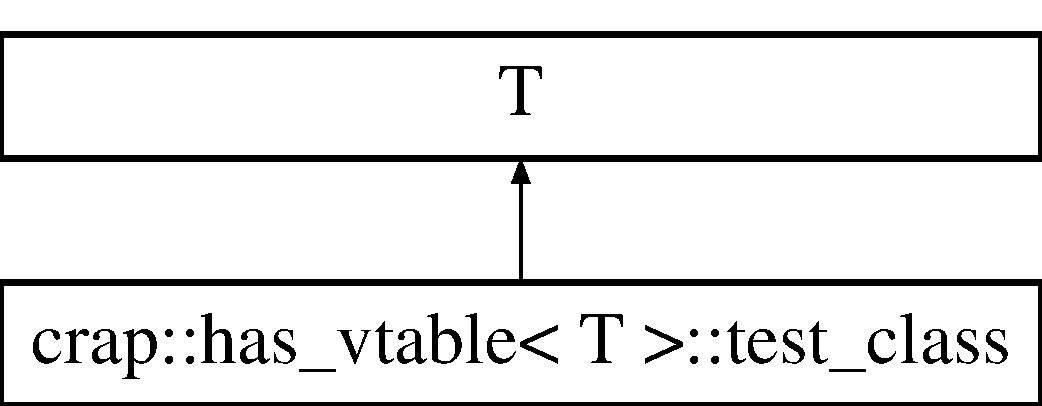
\includegraphics[height=2.000000cm]{structcrap_1_1has__vtable_1_1test__class}
\end{center}
\end{figure}
\subsection*{Public Member Functions}
\begin{DoxyCompactItemize}
\item 
\hyperlink{structcrap_1_1has__vtable_1_1test__class_a6e4ee5125a96ae1e7d9ca1c64c4cd8fe}{test\-\_\-class} ()
\item 
virtual \hyperlink{structcrap_1_1has__vtable_1_1test__class_ac1ec56b0a5223d91214a50cba6acd28f}{$\sim$test\-\_\-class} ()
\end{DoxyCompactItemize}


\subsection{Constructor \& Destructor Documentation}
\hypertarget{structcrap_1_1has__vtable_1_1test__class_a6e4ee5125a96ae1e7d9ca1c64c4cd8fe}{\index{crap\-::has\-\_\-vtable\-::test\-\_\-class@{crap\-::has\-\_\-vtable\-::test\-\_\-class}!test\-\_\-class@{test\-\_\-class}}
\index{test\-\_\-class@{test\-\_\-class}!crap::has_vtable::test_class@{crap\-::has\-\_\-vtable\-::test\-\_\-class}}
\subsubsection[{test\-\_\-class}]{\setlength{\rightskip}{0pt plus 5cm}template$<$class T $>$ {\bf crap\-::has\-\_\-vtable}$<$ T $>$\-::test\-\_\-class\-::test\-\_\-class (
\begin{DoxyParamCaption}
{}
\end{DoxyParamCaption}
)\hspace{0.3cm}{\ttfamily [inline]}}}\label{structcrap_1_1has__vtable_1_1test__class_a6e4ee5125a96ae1e7d9ca1c64c4cd8fe}
\hypertarget{structcrap_1_1has__vtable_1_1test__class_ac1ec56b0a5223d91214a50cba6acd28f}{\index{crap\-::has\-\_\-vtable\-::test\-\_\-class@{crap\-::has\-\_\-vtable\-::test\-\_\-class}!$\sim$test\-\_\-class@{$\sim$test\-\_\-class}}
\index{$\sim$test\-\_\-class@{$\sim$test\-\_\-class}!crap::has_vtable::test_class@{crap\-::has\-\_\-vtable\-::test\-\_\-class}}
\subsubsection[{$\sim$test\-\_\-class}]{\setlength{\rightskip}{0pt plus 5cm}template$<$class T $>$ virtual {\bf crap\-::has\-\_\-vtable}$<$ T $>$\-::test\-\_\-class\-::$\sim$test\-\_\-class (
\begin{DoxyParamCaption}
{}
\end{DoxyParamCaption}
)\hspace{0.3cm}{\ttfamily [virtual]}}}\label{structcrap_1_1has__vtable_1_1test__class_ac1ec56b0a5223d91214a50cba6acd28f}


The documentation for this struct was generated from the following file\-:\begin{DoxyCompactItemize}
\item 
/mnt/windows/data/\-Programmierung/\-C\-R\-A\-P/src/crap/control/\hyperlink{checkvtable_8h}{checkvtable.\-h}\end{DoxyCompactItemize}

\hypertarget{classcrap_1_1thread}{\section{crap\-:\-:thread Class Reference}
\label{classcrap_1_1thread}\index{crap\-::thread@{crap\-::thread}}
}


{\ttfamily \#include $<$thread.\-h$>$}

\subsection*{Public Member Functions}
\begin{DoxyCompactItemize}
\item 
\hyperlink{classcrap_1_1thread_a1b63c7afb1297407aa5cd56d13b6ba48}{thread} (\hyperlink{classcrap_1_1runnable}{runnable} $\ast$runner)
\item 
\hyperlink{classcrap_1_1thread_af45b231794472e9a64a626a7f5a60d3d}{$\sim$thread} ()
\item 
bool \hyperlink{classcrap_1_1thread_a6fa8d75e1bb7c3446804b93400ffd54a}{wait\-\_\-for\-\_\-thread} () const 
\item 
bool \hyperlink{classcrap_1_1thread_a1302dbc7afe6f5192af2e09f8d759981}{kill\-\_\-thread} ()
\item 
\hyperlink{threading_8h_a14c0f3061b88e46a595ca858fed22b03}{T\-H\-R\-E\-A\-D\-\_\-\-H\-A\-N\-D\-L\-E} \hyperlink{classcrap_1_1thread_aed4668b9e26eaf0d3e53871bc109df04}{thread\-\_\-id} ()
\end{DoxyCompactItemize}


\subsection{Constructor \& Destructor Documentation}
\hypertarget{classcrap_1_1thread_a1b63c7afb1297407aa5cd56d13b6ba48}{\index{crap\-::thread@{crap\-::thread}!thread@{thread}}
\index{thread@{thread}!crap::thread@{crap\-::thread}}
\subsubsection[{thread}]{\setlength{\rightskip}{0pt plus 5cm}crap\-::thread\-::thread (
\begin{DoxyParamCaption}
\item[{{\bf runnable} $\ast$}]{runner}
\end{DoxyParamCaption}
)}}\label{classcrap_1_1thread_a1b63c7afb1297407aa5cd56d13b6ba48}
\hypertarget{classcrap_1_1thread_af45b231794472e9a64a626a7f5a60d3d}{\index{crap\-::thread@{crap\-::thread}!$\sim$thread@{$\sim$thread}}
\index{$\sim$thread@{$\sim$thread}!crap::thread@{crap\-::thread}}
\subsubsection[{$\sim$thread}]{\setlength{\rightskip}{0pt plus 5cm}crap\-::thread\-::$\sim$thread (
\begin{DoxyParamCaption}
{}
\end{DoxyParamCaption}
)}}\label{classcrap_1_1thread_af45b231794472e9a64a626a7f5a60d3d}


\subsection{Member Function Documentation}
\hypertarget{classcrap_1_1thread_a1302dbc7afe6f5192af2e09f8d759981}{\index{crap\-::thread@{crap\-::thread}!kill\-\_\-thread@{kill\-\_\-thread}}
\index{kill\-\_\-thread@{kill\-\_\-thread}!crap::thread@{crap\-::thread}}
\subsubsection[{kill\-\_\-thread}]{\setlength{\rightskip}{0pt plus 5cm}bool crap\-::thread\-::kill\-\_\-thread (
\begin{DoxyParamCaption}
{}
\end{DoxyParamCaption}
)}}\label{classcrap_1_1thread_a1302dbc7afe6f5192af2e09f8d759981}
\hypertarget{classcrap_1_1thread_aed4668b9e26eaf0d3e53871bc109df04}{\index{crap\-::thread@{crap\-::thread}!thread\-\_\-id@{thread\-\_\-id}}
\index{thread\-\_\-id@{thread\-\_\-id}!crap::thread@{crap\-::thread}}
\subsubsection[{thread\-\_\-id}]{\setlength{\rightskip}{0pt plus 5cm}{\bf T\-H\-R\-E\-A\-D\-\_\-\-H\-A\-N\-D\-L\-E} crap\-::thread\-::thread\-\_\-id (
\begin{DoxyParamCaption}
\item[{void}]{}
\end{DoxyParamCaption}
)}}\label{classcrap_1_1thread_aed4668b9e26eaf0d3e53871bc109df04}
\hypertarget{classcrap_1_1thread_a6fa8d75e1bb7c3446804b93400ffd54a}{\index{crap\-::thread@{crap\-::thread}!wait\-\_\-for\-\_\-thread@{wait\-\_\-for\-\_\-thread}}
\index{wait\-\_\-for\-\_\-thread@{wait\-\_\-for\-\_\-thread}!crap::thread@{crap\-::thread}}
\subsubsection[{wait\-\_\-for\-\_\-thread}]{\setlength{\rightskip}{0pt plus 5cm}bool crap\-::thread\-::wait\-\_\-for\-\_\-thread (
\begin{DoxyParamCaption}
{}
\end{DoxyParamCaption}
) const}}\label{classcrap_1_1thread_a6fa8d75e1bb7c3446804b93400ffd54a}


The documentation for this class was generated from the following files\-:\begin{DoxyCompactItemize}
\item 
/mnt/windows/data/\-Programmierung/\-C\-R\-A\-P/src/crap/threading/\hyperlink{thread_8h}{thread.\-h}\item 
/mnt/windows/data/\-Programmierung/\-C\-R\-A\-P/src/crap/threading/\hyperlink{thread_8cpp}{thread.\-cpp}\end{DoxyCompactItemize}

\hypertarget{classcrap_1_1time}{\section{crap\-:\-:time Class Reference}
\label{classcrap_1_1time}\index{crap\-::time@{crap\-::time}}
}


{\ttfamily \#include $<$time.\-h$>$}

\subsection*{Classes}
\begin{DoxyCompactItemize}
\item 
struct \hyperlink{structcrap_1_1time_1_1time__info}{time\-\_\-info}
\end{DoxyCompactItemize}
\subsection*{Public Member Functions}
\begin{DoxyCompactItemize}
\item 
\hyperlink{classcrap_1_1time_a9e759f32d27f43a85c21e496205cbea2}{$\sim$time} ()
\item 
\hyperlink{structcrap_1_1time_1_1time__info}{time\-\_\-info} \hyperlink{classcrap_1_1time_a7ebddc1f0416219b1548b8e5fa65f939}{current\-\_\-time} (void)
\item 
\hyperlink{types_8h_a3f7e2bcbb0b4c338f3c4f6c937cd4234}{u64} \hyperlink{classcrap_1_1time_a8f2b003ac30848e9419e19649ca1b509}{current\-\_\-tick} (void)
\item 
\hyperlink{namespacecrap_a502636a1c5819e8500d07deed797ef9f}{string64} \hyperlink{classcrap_1_1time_a7169f0086d7b43744135268d43b77d90}{week\-\_\-day\-\_\-name} (\hyperlink{types_8h_a92c50087ca0e64fa93fc59402c55f8ca}{u8} id)
\item 
\hyperlink{namespacecrap_a502636a1c5819e8500d07deed797ef9f}{string64} \hyperlink{classcrap_1_1time_a7dffd26830f384f33e53cca0a67358b4}{month\-\_\-name} (\hyperlink{types_8h_a92c50087ca0e64fa93fc59402c55f8ca}{u8} id)
\end{DoxyCompactItemize}
\subsection*{Static Public Member Functions}
\begin{DoxyCompactItemize}
\item 
static \hyperlink{classcrap_1_1time}{time} \& \hyperlink{classcrap_1_1time_a6691ce57d6fd0047d8e6d564b6bca030}{instance} (void)
\end{DoxyCompactItemize}
\subsection*{Static Public Attributes}
\begin{DoxyCompactItemize}
\item 
static const \hyperlink{types_8h_afaa62991928fb9fb18ff0db62a040aba}{u32} \hyperlink{classcrap_1_1time_a51db2a5e9626facf398670af5aff1a2d}{T\-I\-C\-K\-S\-\_\-\-P\-E\-R\-\_\-\-S\-E\-C\-O\-N\-D} = C\-L\-O\-C\-K\-S\-\_\-\-P\-E\-R\-\_\-\-S\-E\-C
\end{DoxyCompactItemize}


\subsection{Constructor \& Destructor Documentation}
\hypertarget{classcrap_1_1time_a9e759f32d27f43a85c21e496205cbea2}{\index{crap\-::time@{crap\-::time}!$\sim$time@{$\sim$time}}
\index{$\sim$time@{$\sim$time}!crap::time@{crap\-::time}}
\subsubsection[{$\sim$time}]{\setlength{\rightskip}{0pt plus 5cm}crap\-::time\-::$\sim$time (
\begin{DoxyParamCaption}
\item[{void}]{}
\end{DoxyParamCaption}
)}}\label{classcrap_1_1time_a9e759f32d27f43a85c21e496205cbea2}


\subsection{Member Function Documentation}
\hypertarget{classcrap_1_1time_a8f2b003ac30848e9419e19649ca1b509}{\index{crap\-::time@{crap\-::time}!current\-\_\-tick@{current\-\_\-tick}}
\index{current\-\_\-tick@{current\-\_\-tick}!crap::time@{crap\-::time}}
\subsubsection[{current\-\_\-tick}]{\setlength{\rightskip}{0pt plus 5cm}{\bf u64} crap\-::time\-::current\-\_\-tick (
\begin{DoxyParamCaption}
\item[{void}]{}
\end{DoxyParamCaption}
)}}\label{classcrap_1_1time_a8f2b003ac30848e9419e19649ca1b509}
\hypertarget{classcrap_1_1time_a7ebddc1f0416219b1548b8e5fa65f939}{\index{crap\-::time@{crap\-::time}!current\-\_\-time@{current\-\_\-time}}
\index{current\-\_\-time@{current\-\_\-time}!crap::time@{crap\-::time}}
\subsubsection[{current\-\_\-time}]{\setlength{\rightskip}{0pt plus 5cm}{\bf time\-::time\-\_\-info} crap\-::time\-::current\-\_\-time (
\begin{DoxyParamCaption}
\item[{void}]{}
\end{DoxyParamCaption}
)}}\label{classcrap_1_1time_a7ebddc1f0416219b1548b8e5fa65f939}
\hypertarget{classcrap_1_1time_a6691ce57d6fd0047d8e6d564b6bca030}{\index{crap\-::time@{crap\-::time}!instance@{instance}}
\index{instance@{instance}!crap::time@{crap\-::time}}
\subsubsection[{instance}]{\setlength{\rightskip}{0pt plus 5cm}{\bf time} \& crap\-::time\-::instance (
\begin{DoxyParamCaption}
\item[{void}]{}
\end{DoxyParamCaption}
)\hspace{0.3cm}{\ttfamily [static]}}}\label{classcrap_1_1time_a6691ce57d6fd0047d8e6d564b6bca030}
\hypertarget{classcrap_1_1time_a7dffd26830f384f33e53cca0a67358b4}{\index{crap\-::time@{crap\-::time}!month\-\_\-name@{month\-\_\-name}}
\index{month\-\_\-name@{month\-\_\-name}!crap::time@{crap\-::time}}
\subsubsection[{month\-\_\-name}]{\setlength{\rightskip}{0pt plus 5cm}{\bf string64} crap\-::time\-::month\-\_\-name (
\begin{DoxyParamCaption}
\item[{{\bf u8}}]{id}
\end{DoxyParamCaption}
)}}\label{classcrap_1_1time_a7dffd26830f384f33e53cca0a67358b4}
\hypertarget{classcrap_1_1time_a7169f0086d7b43744135268d43b77d90}{\index{crap\-::time@{crap\-::time}!week\-\_\-day\-\_\-name@{week\-\_\-day\-\_\-name}}
\index{week\-\_\-day\-\_\-name@{week\-\_\-day\-\_\-name}!crap::time@{crap\-::time}}
\subsubsection[{week\-\_\-day\-\_\-name}]{\setlength{\rightskip}{0pt plus 5cm}{\bf string64} crap\-::time\-::week\-\_\-day\-\_\-name (
\begin{DoxyParamCaption}
\item[{{\bf u8}}]{id}
\end{DoxyParamCaption}
)}}\label{classcrap_1_1time_a7169f0086d7b43744135268d43b77d90}


\subsection{Member Data Documentation}
\hypertarget{classcrap_1_1time_a51db2a5e9626facf398670af5aff1a2d}{\index{crap\-::time@{crap\-::time}!T\-I\-C\-K\-S\-\_\-\-P\-E\-R\-\_\-\-S\-E\-C\-O\-N\-D@{T\-I\-C\-K\-S\-\_\-\-P\-E\-R\-\_\-\-S\-E\-C\-O\-N\-D}}
\index{T\-I\-C\-K\-S\-\_\-\-P\-E\-R\-\_\-\-S\-E\-C\-O\-N\-D@{T\-I\-C\-K\-S\-\_\-\-P\-E\-R\-\_\-\-S\-E\-C\-O\-N\-D}!crap::time@{crap\-::time}}
\subsubsection[{T\-I\-C\-K\-S\-\_\-\-P\-E\-R\-\_\-\-S\-E\-C\-O\-N\-D}]{\setlength{\rightskip}{0pt plus 5cm}const {\bf u32} crap\-::time\-::\-T\-I\-C\-K\-S\-\_\-\-P\-E\-R\-\_\-\-S\-E\-C\-O\-N\-D = C\-L\-O\-C\-K\-S\-\_\-\-P\-E\-R\-\_\-\-S\-E\-C\hspace{0.3cm}{\ttfamily [static]}}}\label{classcrap_1_1time_a51db2a5e9626facf398670af5aff1a2d}


The documentation for this class was generated from the following files\-:\begin{DoxyCompactItemize}
\item 
/mnt/windows/data/\-Programmierung/\-C\-R\-A\-P/src/crap/control/\hyperlink{time_8h}{time.\-h}\item 
/mnt/windows/data/\-Programmierung/\-C\-R\-A\-P/src/crap/control/\hyperlink{time_8cpp}{time.\-cpp}\end{DoxyCompactItemize}

\hypertarget{structcrap_1_1time_1_1time__info}{\section{crap\-:\-:time\-:\-:time\-\_\-info Struct Reference}
\label{structcrap_1_1time_1_1time__info}\index{crap\-::time\-::time\-\_\-info@{crap\-::time\-::time\-\_\-info}}
}


{\ttfamily \#include $<$time.\-h$>$}

\subsection*{Public Member Functions}
\begin{DoxyCompactItemize}
\item 
\hyperlink{structcrap_1_1time_1_1time__info_adc92ed9049658fabce02dbdfc4479a17}{time\-\_\-info} (\hyperlink{types_8h_a92c50087ca0e64fa93fc59402c55f8ca}{u8} s, \hyperlink{types_8h_a92c50087ca0e64fa93fc59402c55f8ca}{u8} m, \hyperlink{types_8h_a92c50087ca0e64fa93fc59402c55f8ca}{u8} h, \hyperlink{types_8h_a92c50087ca0e64fa93fc59402c55f8ca}{u8} d, \hyperlink{types_8h_a92c50087ca0e64fa93fc59402c55f8ca}{u8} M, \hyperlink{types_8h_ace9d960e74685e2cd84b36132dbbf8aa}{u16} Y, \hyperlink{types_8h_a92c50087ca0e64fa93fc59402c55f8ca}{u8} w, \hyperlink{types_8h_ace9d960e74685e2cd84b36132dbbf8aa}{u16} y)
\end{DoxyCompactItemize}
\subsection*{Public Attributes}
\begin{DoxyCompactItemize}
\item 
\hyperlink{types_8h_a92c50087ca0e64fa93fc59402c55f8ca}{u8} \hyperlink{structcrap_1_1time_1_1time__info_a9a09f309a2f81e1a8fc5acd2b1876bf5}{seconds}
\item 
\hyperlink{types_8h_a92c50087ca0e64fa93fc59402c55f8ca}{u8} \hyperlink{structcrap_1_1time_1_1time__info_aaf56c55fb9d93178522e98d4f2a8b557}{minutes}
\item 
\hyperlink{types_8h_a92c50087ca0e64fa93fc59402c55f8ca}{u8} \hyperlink{structcrap_1_1time_1_1time__info_a956dc012f40205e9f834d8802feb9642}{hours}
\item 
\hyperlink{types_8h_a92c50087ca0e64fa93fc59402c55f8ca}{u8} \hyperlink{structcrap_1_1time_1_1time__info_adb80a0c67c8f89e4399e64364f5e7c3a}{day}
\item 
\hyperlink{types_8h_a92c50087ca0e64fa93fc59402c55f8ca}{u8} \hyperlink{structcrap_1_1time_1_1time__info_a69449bc6ce083b864f4a3acbf599b58a}{month}
\item 
\hyperlink{types_8h_ace9d960e74685e2cd84b36132dbbf8aa}{u16} \hyperlink{structcrap_1_1time_1_1time__info_aab40e5fecd12881e84dea8449c7dc7b2}{year}
\item 
\hyperlink{types_8h_a92c50087ca0e64fa93fc59402c55f8ca}{u8} \hyperlink{structcrap_1_1time_1_1time__info_a53f401c11fa1b828ab59d9f46c31939d}{weekday}
\item 
\hyperlink{types_8h_ace9d960e74685e2cd84b36132dbbf8aa}{u16} \hyperlink{structcrap_1_1time_1_1time__info_a286c0bab84aba2063b13770ab235e4e3}{yearday}
\end{DoxyCompactItemize}


\subsection{Constructor \& Destructor Documentation}
\hypertarget{structcrap_1_1time_1_1time__info_adc92ed9049658fabce02dbdfc4479a17}{\index{crap\-::time\-::time\-\_\-info@{crap\-::time\-::time\-\_\-info}!time\-\_\-info@{time\-\_\-info}}
\index{time\-\_\-info@{time\-\_\-info}!crap::time::time_info@{crap\-::time\-::time\-\_\-info}}
\subsubsection[{time\-\_\-info}]{\setlength{\rightskip}{0pt plus 5cm}crap\-::time\-::time\-\_\-info\-::time\-\_\-info (
\begin{DoxyParamCaption}
\item[{{\bf u8}}]{s, }
\item[{{\bf u8}}]{m, }
\item[{{\bf u8}}]{h, }
\item[{{\bf u8}}]{d, }
\item[{{\bf u8}}]{M, }
\item[{{\bf u16}}]{Y, }
\item[{{\bf u8}}]{w, }
\item[{{\bf u16}}]{y}
\end{DoxyParamCaption}
)\hspace{0.3cm}{\ttfamily [inline]}}}\label{structcrap_1_1time_1_1time__info_adc92ed9049658fabce02dbdfc4479a17}


\subsection{Member Data Documentation}
\hypertarget{structcrap_1_1time_1_1time__info_adb80a0c67c8f89e4399e64364f5e7c3a}{\index{crap\-::time\-::time\-\_\-info@{crap\-::time\-::time\-\_\-info}!day@{day}}
\index{day@{day}!crap::time::time_info@{crap\-::time\-::time\-\_\-info}}
\subsubsection[{day}]{\setlength{\rightskip}{0pt plus 5cm}{\bf u8} crap\-::time\-::time\-\_\-info\-::day}}\label{structcrap_1_1time_1_1time__info_adb80a0c67c8f89e4399e64364f5e7c3a}
\hypertarget{structcrap_1_1time_1_1time__info_a956dc012f40205e9f834d8802feb9642}{\index{crap\-::time\-::time\-\_\-info@{crap\-::time\-::time\-\_\-info}!hours@{hours}}
\index{hours@{hours}!crap::time::time_info@{crap\-::time\-::time\-\_\-info}}
\subsubsection[{hours}]{\setlength{\rightskip}{0pt plus 5cm}{\bf u8} crap\-::time\-::time\-\_\-info\-::hours}}\label{structcrap_1_1time_1_1time__info_a956dc012f40205e9f834d8802feb9642}
\hypertarget{structcrap_1_1time_1_1time__info_aaf56c55fb9d93178522e98d4f2a8b557}{\index{crap\-::time\-::time\-\_\-info@{crap\-::time\-::time\-\_\-info}!minutes@{minutes}}
\index{minutes@{minutes}!crap::time::time_info@{crap\-::time\-::time\-\_\-info}}
\subsubsection[{minutes}]{\setlength{\rightskip}{0pt plus 5cm}{\bf u8} crap\-::time\-::time\-\_\-info\-::minutes}}\label{structcrap_1_1time_1_1time__info_aaf56c55fb9d93178522e98d4f2a8b557}
\hypertarget{structcrap_1_1time_1_1time__info_a69449bc6ce083b864f4a3acbf599b58a}{\index{crap\-::time\-::time\-\_\-info@{crap\-::time\-::time\-\_\-info}!month@{month}}
\index{month@{month}!crap::time::time_info@{crap\-::time\-::time\-\_\-info}}
\subsubsection[{month}]{\setlength{\rightskip}{0pt plus 5cm}{\bf u8} crap\-::time\-::time\-\_\-info\-::month}}\label{structcrap_1_1time_1_1time__info_a69449bc6ce083b864f4a3acbf599b58a}
\hypertarget{structcrap_1_1time_1_1time__info_a9a09f309a2f81e1a8fc5acd2b1876bf5}{\index{crap\-::time\-::time\-\_\-info@{crap\-::time\-::time\-\_\-info}!seconds@{seconds}}
\index{seconds@{seconds}!crap::time::time_info@{crap\-::time\-::time\-\_\-info}}
\subsubsection[{seconds}]{\setlength{\rightskip}{0pt plus 5cm}{\bf u8} crap\-::time\-::time\-\_\-info\-::seconds}}\label{structcrap_1_1time_1_1time__info_a9a09f309a2f81e1a8fc5acd2b1876bf5}
\hypertarget{structcrap_1_1time_1_1time__info_a53f401c11fa1b828ab59d9f46c31939d}{\index{crap\-::time\-::time\-\_\-info@{crap\-::time\-::time\-\_\-info}!weekday@{weekday}}
\index{weekday@{weekday}!crap::time::time_info@{crap\-::time\-::time\-\_\-info}}
\subsubsection[{weekday}]{\setlength{\rightskip}{0pt plus 5cm}{\bf u8} crap\-::time\-::time\-\_\-info\-::weekday}}\label{structcrap_1_1time_1_1time__info_a53f401c11fa1b828ab59d9f46c31939d}
\hypertarget{structcrap_1_1time_1_1time__info_aab40e5fecd12881e84dea8449c7dc7b2}{\index{crap\-::time\-::time\-\_\-info@{crap\-::time\-::time\-\_\-info}!year@{year}}
\index{year@{year}!crap::time::time_info@{crap\-::time\-::time\-\_\-info}}
\subsubsection[{year}]{\setlength{\rightskip}{0pt plus 5cm}{\bf u16} crap\-::time\-::time\-\_\-info\-::year}}\label{structcrap_1_1time_1_1time__info_aab40e5fecd12881e84dea8449c7dc7b2}
\hypertarget{structcrap_1_1time_1_1time__info_a286c0bab84aba2063b13770ab235e4e3}{\index{crap\-::time\-::time\-\_\-info@{crap\-::time\-::time\-\_\-info}!yearday@{yearday}}
\index{yearday@{yearday}!crap::time::time_info@{crap\-::time\-::time\-\_\-info}}
\subsubsection[{yearday}]{\setlength{\rightskip}{0pt plus 5cm}{\bf u16} crap\-::time\-::time\-\_\-info\-::yearday}}\label{structcrap_1_1time_1_1time__info_a286c0bab84aba2063b13770ab235e4e3}


The documentation for this struct was generated from the following file\-:\begin{DoxyCompactItemize}
\item 
/mnt/windows/data/\-Programmierung/\-C\-R\-A\-P/src/crap/control/\hyperlink{time_8h}{time.\-h}\end{DoxyCompactItemize}

\hypertarget{structcrap_1_1binary__tree_1_1tree__iterator}{\section{crap\-:\-:binary\-\_\-tree$<$ T, C, A $>$\-:\-:tree\-\_\-iterator Struct Reference}
\label{structcrap_1_1binary__tree_1_1tree__iterator}\index{crap\-::binary\-\_\-tree$<$ T, C, A $>$\-::tree\-\_\-iterator@{crap\-::binary\-\_\-tree$<$ T, C, A $>$\-::tree\-\_\-iterator}}
}


{\ttfamily \#include $<$binarytree.\-h$>$}

\subsection*{Public Member Functions}
\begin{DoxyCompactItemize}
\item 
\hyperlink{structcrap_1_1binary__tree_1_1tree__iterator_a3aa9d13fa33e42be6fb83fd91413dfd7}{tree\-\_\-iterator} (void)
\item 
\hyperlink{structcrap_1_1binary__tree_1_1tree__iterator_a495aba5dfcdae2ba041d45bd136314a7}{tree\-\_\-iterator} (\hyperlink{classcrap_1_1binary__tree_a04d7ea4aa1c1cc5bdd06cbdf3d537076}{node\-\_\-pointer} element)
\item 
\hyperlink{structcrap_1_1binary__tree_1_1tree__iterator_a2a4b32aa6da04ceb8374f57b69a49038}{tree\-\_\-iterator} (const \hyperlink{structcrap_1_1binary__tree_1_1tree__iterator}{tree\-\_\-iterator} \&other)
\item 
\hyperlink{structcrap_1_1binary__tree_1_1tree__iterator}{tree\-\_\-iterator} \& \hyperlink{structcrap_1_1binary__tree_1_1tree__iterator_af9f561a466424592a6edf5733498c9d6}{operator=} (const \hyperlink{structcrap_1_1binary__tree_1_1tree__iterator}{tree\-\_\-iterator} \&other)
\item 
void \hyperlink{structcrap_1_1binary__tree_1_1tree__iterator_afd8692cd1d3cfcfe9848457f8acea6bf}{operator++} (void)
\item 
void \hyperlink{structcrap_1_1binary__tree_1_1tree__iterator_ad27ad8d39ddc2f87545bec7ffa5fd506}{operator-\/-\/} (void)
\item 
bool \hyperlink{structcrap_1_1binary__tree_1_1tree__iterator_aa683328f2810df0e07255b6ad26903d3}{operator==} (const \hyperlink{structcrap_1_1binary__tree_1_1tree__iterator}{tree\-\_\-iterator} \&other) const 
\item 
bool \hyperlink{structcrap_1_1binary__tree_1_1tree__iterator_a70cff44fb6c88e8b0ae537809637ce8b}{operator!=} (const \hyperlink{structcrap_1_1binary__tree_1_1tree__iterator}{tree\-\_\-iterator} \&other) const 
\item 
\hyperlink{classcrap_1_1binary__tree_a04d7ea4aa1c1cc5bdd06cbdf3d537076}{node\-\_\-pointer} \hyperlink{structcrap_1_1binary__tree_1_1tree__iterator_adeb2a8902e8885c3faa46a9ea5e35e29}{operator-\/$>$} (void)
\item 
T \& \hyperlink{structcrap_1_1binary__tree_1_1tree__iterator_a0bb3866a5e0de5cd1e20b2dcf248c366}{operator$\ast$} (void)
\item 
const T \& \hyperlink{structcrap_1_1binary__tree_1_1tree__iterator_a652a605ba08402e7db3341b09e1fcdcf}{operator$\ast$} (void) const 
\item 
\hyperlink{classcrap_1_1binary__tree_a04d7ea4aa1c1cc5bdd06cbdf3d537076}{node\-\_\-pointer} \hyperlink{structcrap_1_1binary__tree_1_1tree__iterator_ad307aef0e2bf1ab55e8d1e3e63608bc7}{ptr} (void) const 
\end{DoxyCompactItemize}


\subsection{Constructor \& Destructor Documentation}
\hypertarget{structcrap_1_1binary__tree_1_1tree__iterator_a3aa9d13fa33e42be6fb83fd91413dfd7}{\index{crap\-::binary\-\_\-tree\-::tree\-\_\-iterator@{crap\-::binary\-\_\-tree\-::tree\-\_\-iterator}!tree\-\_\-iterator@{tree\-\_\-iterator}}
\index{tree\-\_\-iterator@{tree\-\_\-iterator}!crap::binary_tree::tree_iterator@{crap\-::binary\-\_\-tree\-::tree\-\_\-iterator}}
\subsubsection[{tree\-\_\-iterator}]{\setlength{\rightskip}{0pt plus 5cm}template$<$class T, class C = crap\-::less$<$\-T$>$, class A = crap\-::allocator\-\_\-default$<$tree\-\_\-node$<$\-T,\-C$>$ $>$$>$ {\bf crap\-::binary\-\_\-tree}$<$ T, C, A $>$\-::tree\-\_\-iterator\-::tree\-\_\-iterator (
\begin{DoxyParamCaption}
\item[{void}]{}
\end{DoxyParamCaption}
)\hspace{0.3cm}{\ttfamily [inline]}}}\label{structcrap_1_1binary__tree_1_1tree__iterator_a3aa9d13fa33e42be6fb83fd91413dfd7}
\hypertarget{structcrap_1_1binary__tree_1_1tree__iterator_a495aba5dfcdae2ba041d45bd136314a7}{\index{crap\-::binary\-\_\-tree\-::tree\-\_\-iterator@{crap\-::binary\-\_\-tree\-::tree\-\_\-iterator}!tree\-\_\-iterator@{tree\-\_\-iterator}}
\index{tree\-\_\-iterator@{tree\-\_\-iterator}!crap::binary_tree::tree_iterator@{crap\-::binary\-\_\-tree\-::tree\-\_\-iterator}}
\subsubsection[{tree\-\_\-iterator}]{\setlength{\rightskip}{0pt plus 5cm}template$<$class T, class C = crap\-::less$<$\-T$>$, class A = crap\-::allocator\-\_\-default$<$tree\-\_\-node$<$\-T,\-C$>$ $>$$>$ {\bf crap\-::binary\-\_\-tree}$<$ T, C, A $>$\-::tree\-\_\-iterator\-::tree\-\_\-iterator (
\begin{DoxyParamCaption}
\item[{{\bf node\-\_\-pointer}}]{element}
\end{DoxyParamCaption}
)\hspace{0.3cm}{\ttfamily [inline]}}}\label{structcrap_1_1binary__tree_1_1tree__iterator_a495aba5dfcdae2ba041d45bd136314a7}
\hypertarget{structcrap_1_1binary__tree_1_1tree__iterator_a2a4b32aa6da04ceb8374f57b69a49038}{\index{crap\-::binary\-\_\-tree\-::tree\-\_\-iterator@{crap\-::binary\-\_\-tree\-::tree\-\_\-iterator}!tree\-\_\-iterator@{tree\-\_\-iterator}}
\index{tree\-\_\-iterator@{tree\-\_\-iterator}!crap::binary_tree::tree_iterator@{crap\-::binary\-\_\-tree\-::tree\-\_\-iterator}}
\subsubsection[{tree\-\_\-iterator}]{\setlength{\rightskip}{0pt plus 5cm}template$<$class T, class C = crap\-::less$<$\-T$>$, class A = crap\-::allocator\-\_\-default$<$tree\-\_\-node$<$\-T,\-C$>$ $>$$>$ {\bf crap\-::binary\-\_\-tree}$<$ T, C, A $>$\-::tree\-\_\-iterator\-::tree\-\_\-iterator (
\begin{DoxyParamCaption}
\item[{const {\bf tree\-\_\-iterator} \&}]{other}
\end{DoxyParamCaption}
)\hspace{0.3cm}{\ttfamily [inline]}}}\label{structcrap_1_1binary__tree_1_1tree__iterator_a2a4b32aa6da04ceb8374f57b69a49038}


\subsection{Member Function Documentation}
\hypertarget{structcrap_1_1binary__tree_1_1tree__iterator_a70cff44fb6c88e8b0ae537809637ce8b}{\index{crap\-::binary\-\_\-tree\-::tree\-\_\-iterator@{crap\-::binary\-\_\-tree\-::tree\-\_\-iterator}!operator!=@{operator!=}}
\index{operator!=@{operator!=}!crap::binary_tree::tree_iterator@{crap\-::binary\-\_\-tree\-::tree\-\_\-iterator}}
\subsubsection[{operator!=}]{\setlength{\rightskip}{0pt plus 5cm}template$<$class T, class C = crap\-::less$<$\-T$>$, class A = crap\-::allocator\-\_\-default$<$tree\-\_\-node$<$\-T,\-C$>$ $>$$>$ bool {\bf crap\-::binary\-\_\-tree}$<$ T, C, A $>$\-::tree\-\_\-iterator\-::operator!= (
\begin{DoxyParamCaption}
\item[{const {\bf tree\-\_\-iterator} \&}]{other}
\end{DoxyParamCaption}
) const\hspace{0.3cm}{\ttfamily [inline]}}}\label{structcrap_1_1binary__tree_1_1tree__iterator_a70cff44fb6c88e8b0ae537809637ce8b}
\hypertarget{structcrap_1_1binary__tree_1_1tree__iterator_a0bb3866a5e0de5cd1e20b2dcf248c366}{\index{crap\-::binary\-\_\-tree\-::tree\-\_\-iterator@{crap\-::binary\-\_\-tree\-::tree\-\_\-iterator}!operator$\ast$@{operator$\ast$}}
\index{operator$\ast$@{operator$\ast$}!crap::binary_tree::tree_iterator@{crap\-::binary\-\_\-tree\-::tree\-\_\-iterator}}
\subsubsection[{operator$\ast$}]{\setlength{\rightskip}{0pt plus 5cm}template$<$class T, class C = crap\-::less$<$\-T$>$, class A = crap\-::allocator\-\_\-default$<$tree\-\_\-node$<$\-T,\-C$>$ $>$$>$ T\& {\bf crap\-::binary\-\_\-tree}$<$ T, C, A $>$\-::tree\-\_\-iterator\-::operator$\ast$ (
\begin{DoxyParamCaption}
\item[{void}]{}
\end{DoxyParamCaption}
)\hspace{0.3cm}{\ttfamily [inline]}}}\label{structcrap_1_1binary__tree_1_1tree__iterator_a0bb3866a5e0de5cd1e20b2dcf248c366}
\hypertarget{structcrap_1_1binary__tree_1_1tree__iterator_a652a605ba08402e7db3341b09e1fcdcf}{\index{crap\-::binary\-\_\-tree\-::tree\-\_\-iterator@{crap\-::binary\-\_\-tree\-::tree\-\_\-iterator}!operator$\ast$@{operator$\ast$}}
\index{operator$\ast$@{operator$\ast$}!crap::binary_tree::tree_iterator@{crap\-::binary\-\_\-tree\-::tree\-\_\-iterator}}
\subsubsection[{operator$\ast$}]{\setlength{\rightskip}{0pt plus 5cm}template$<$class T, class C = crap\-::less$<$\-T$>$, class A = crap\-::allocator\-\_\-default$<$tree\-\_\-node$<$\-T,\-C$>$ $>$$>$ const T\& {\bf crap\-::binary\-\_\-tree}$<$ T, C, A $>$\-::tree\-\_\-iterator\-::operator$\ast$ (
\begin{DoxyParamCaption}
\item[{void}]{}
\end{DoxyParamCaption}
) const\hspace{0.3cm}{\ttfamily [inline]}}}\label{structcrap_1_1binary__tree_1_1tree__iterator_a652a605ba08402e7db3341b09e1fcdcf}
\hypertarget{structcrap_1_1binary__tree_1_1tree__iterator_afd8692cd1d3cfcfe9848457f8acea6bf}{\index{crap\-::binary\-\_\-tree\-::tree\-\_\-iterator@{crap\-::binary\-\_\-tree\-::tree\-\_\-iterator}!operator++@{operator++}}
\index{operator++@{operator++}!crap::binary_tree::tree_iterator@{crap\-::binary\-\_\-tree\-::tree\-\_\-iterator}}
\subsubsection[{operator++}]{\setlength{\rightskip}{0pt plus 5cm}template$<$class T, class C = crap\-::less$<$\-T$>$, class A = crap\-::allocator\-\_\-default$<$tree\-\_\-node$<$\-T,\-C$>$ $>$$>$ void {\bf crap\-::binary\-\_\-tree}$<$ T, C, A $>$\-::tree\-\_\-iterator\-::operator++ (
\begin{DoxyParamCaption}
\item[{void}]{}
\end{DoxyParamCaption}
)\hspace{0.3cm}{\ttfamily [inline]}}}\label{structcrap_1_1binary__tree_1_1tree__iterator_afd8692cd1d3cfcfe9848457f8acea6bf}
\hypertarget{structcrap_1_1binary__tree_1_1tree__iterator_ad27ad8d39ddc2f87545bec7ffa5fd506}{\index{crap\-::binary\-\_\-tree\-::tree\-\_\-iterator@{crap\-::binary\-\_\-tree\-::tree\-\_\-iterator}!operator-\/-\/@{operator-\/-\/}}
\index{operator-\/-\/@{operator-\/-\/}!crap::binary_tree::tree_iterator@{crap\-::binary\-\_\-tree\-::tree\-\_\-iterator}}
\subsubsection[{operator-\/-\/}]{\setlength{\rightskip}{0pt plus 5cm}template$<$class T, class C = crap\-::less$<$\-T$>$, class A = crap\-::allocator\-\_\-default$<$tree\-\_\-node$<$\-T,\-C$>$ $>$$>$ void {\bf crap\-::binary\-\_\-tree}$<$ T, C, A $>$\-::tree\-\_\-iterator\-::operator-\/-\/ (
\begin{DoxyParamCaption}
\item[{void}]{}
\end{DoxyParamCaption}
)\hspace{0.3cm}{\ttfamily [inline]}}}\label{structcrap_1_1binary__tree_1_1tree__iterator_ad27ad8d39ddc2f87545bec7ffa5fd506}
\hypertarget{structcrap_1_1binary__tree_1_1tree__iterator_adeb2a8902e8885c3faa46a9ea5e35e29}{\index{crap\-::binary\-\_\-tree\-::tree\-\_\-iterator@{crap\-::binary\-\_\-tree\-::tree\-\_\-iterator}!operator-\/$>$@{operator-\/$>$}}
\index{operator-\/$>$@{operator-\/$>$}!crap::binary_tree::tree_iterator@{crap\-::binary\-\_\-tree\-::tree\-\_\-iterator}}
\subsubsection[{operator-\/$>$}]{\setlength{\rightskip}{0pt plus 5cm}template$<$class T, class C = crap\-::less$<$\-T$>$, class A = crap\-::allocator\-\_\-default$<$tree\-\_\-node$<$\-T,\-C$>$ $>$$>$ {\bf node\-\_\-pointer} {\bf crap\-::binary\-\_\-tree}$<$ T, C, A $>$\-::tree\-\_\-iterator\-::operator-\/$>$ (
\begin{DoxyParamCaption}
\item[{void}]{}
\end{DoxyParamCaption}
)\hspace{0.3cm}{\ttfamily [inline]}}}\label{structcrap_1_1binary__tree_1_1tree__iterator_adeb2a8902e8885c3faa46a9ea5e35e29}
\hypertarget{structcrap_1_1binary__tree_1_1tree__iterator_af9f561a466424592a6edf5733498c9d6}{\index{crap\-::binary\-\_\-tree\-::tree\-\_\-iterator@{crap\-::binary\-\_\-tree\-::tree\-\_\-iterator}!operator=@{operator=}}
\index{operator=@{operator=}!crap::binary_tree::tree_iterator@{crap\-::binary\-\_\-tree\-::tree\-\_\-iterator}}
\subsubsection[{operator=}]{\setlength{\rightskip}{0pt plus 5cm}template$<$class T, class C = crap\-::less$<$\-T$>$, class A = crap\-::allocator\-\_\-default$<$tree\-\_\-node$<$\-T,\-C$>$ $>$$>$ {\bf tree\-\_\-iterator}\& {\bf crap\-::binary\-\_\-tree}$<$ T, C, A $>$\-::tree\-\_\-iterator\-::operator= (
\begin{DoxyParamCaption}
\item[{const {\bf tree\-\_\-iterator} \&}]{other}
\end{DoxyParamCaption}
)\hspace{0.3cm}{\ttfamily [inline]}}}\label{structcrap_1_1binary__tree_1_1tree__iterator_af9f561a466424592a6edf5733498c9d6}
\hypertarget{structcrap_1_1binary__tree_1_1tree__iterator_aa683328f2810df0e07255b6ad26903d3}{\index{crap\-::binary\-\_\-tree\-::tree\-\_\-iterator@{crap\-::binary\-\_\-tree\-::tree\-\_\-iterator}!operator==@{operator==}}
\index{operator==@{operator==}!crap::binary_tree::tree_iterator@{crap\-::binary\-\_\-tree\-::tree\-\_\-iterator}}
\subsubsection[{operator==}]{\setlength{\rightskip}{0pt plus 5cm}template$<$class T, class C = crap\-::less$<$\-T$>$, class A = crap\-::allocator\-\_\-default$<$tree\-\_\-node$<$\-T,\-C$>$ $>$$>$ bool {\bf crap\-::binary\-\_\-tree}$<$ T, C, A $>$\-::tree\-\_\-iterator\-::operator== (
\begin{DoxyParamCaption}
\item[{const {\bf tree\-\_\-iterator} \&}]{other}
\end{DoxyParamCaption}
) const\hspace{0.3cm}{\ttfamily [inline]}}}\label{structcrap_1_1binary__tree_1_1tree__iterator_aa683328f2810df0e07255b6ad26903d3}
\hypertarget{structcrap_1_1binary__tree_1_1tree__iterator_ad307aef0e2bf1ab55e8d1e3e63608bc7}{\index{crap\-::binary\-\_\-tree\-::tree\-\_\-iterator@{crap\-::binary\-\_\-tree\-::tree\-\_\-iterator}!ptr@{ptr}}
\index{ptr@{ptr}!crap::binary_tree::tree_iterator@{crap\-::binary\-\_\-tree\-::tree\-\_\-iterator}}
\subsubsection[{ptr}]{\setlength{\rightskip}{0pt plus 5cm}template$<$class T, class C = crap\-::less$<$\-T$>$, class A = crap\-::allocator\-\_\-default$<$tree\-\_\-node$<$\-T,\-C$>$ $>$$>$ {\bf node\-\_\-pointer} {\bf crap\-::binary\-\_\-tree}$<$ T, C, A $>$\-::tree\-\_\-iterator\-::ptr (
\begin{DoxyParamCaption}
\item[{void}]{}
\end{DoxyParamCaption}
) const\hspace{0.3cm}{\ttfamily [inline]}}}\label{structcrap_1_1binary__tree_1_1tree__iterator_ad307aef0e2bf1ab55e8d1e3e63608bc7}


The documentation for this struct was generated from the following file\-:\begin{DoxyCompactItemize}
\item 
/mnt/windows/data/\-Programmierung/\-C\-R\-A\-P/src/crap/container/\hyperlink{binarytree_8h}{binarytree.\-h}\end{DoxyCompactItemize}

\hypertarget{classcrap_1_1tree__map}{\section{crap\-:\-:tree\-\_\-map$<$ T1, T2, C, A $>$ Class Template Reference}
\label{classcrap_1_1tree__map}\index{crap\-::tree\-\_\-map$<$ T1, T2, C, A $>$@{crap\-::tree\-\_\-map$<$ T1, T2, C, A $>$}}
}


using binary tree with pair$<$$>$  




{\ttfamily \#include $<$map.\-h$>$}

Inheritance diagram for crap\-:\-:tree\-\_\-map$<$ T1, T2, C, A $>$\-:\begin{figure}[H]
\begin{center}
\leavevmode
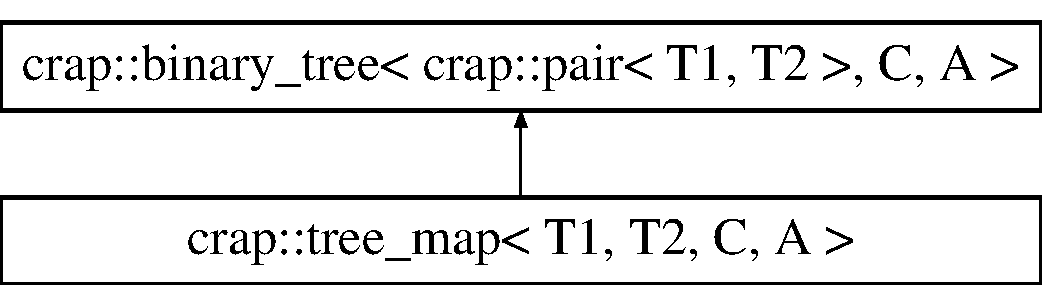
\includegraphics[height=2.000000cm]{classcrap_1_1tree__map}
\end{center}
\end{figure}
\subsection*{Additional Inherited Members}


\subsection{Detailed Description}
\subsubsection*{template$<$class T1, class T2, class C = crap\-::less\-\_\-first$<$\-T1, T2$>$, class A = crap\-::allocator\-\_\-default$<$tree\-\_\-node$<$ pair$<$\-T1, T2$>$ ,\-C$>$ $>$$>$class crap\-::tree\-\_\-map$<$ T1, T2, C, A $>$}

using binary tree with pair$<$$>$ 

The documentation for this class was generated from the following file\-:\begin{DoxyCompactItemize}
\item 
/mnt/windows/data/\-Programmierung/\-C\-R\-A\-P/src/crap/container/\hyperlink{map_8h}{map.\-h}\end{DoxyCompactItemize}

\hypertarget{structcrap_1_1tree__node}{\section{crap\-:\-:tree\-\_\-node$<$ T, C $>$ Struct Template Reference}
\label{structcrap_1_1tree__node}\index{crap\-::tree\-\_\-node$<$ T, C $>$@{crap\-::tree\-\_\-node$<$ T, C $>$}}
}


{\ttfamily \#include $<$treenode.\-h$>$}

\subsection*{Public Types}
\begin{DoxyCompactItemize}
\item 
enum \hyperlink{structcrap_1_1tree__node_a8611158287f75bc048b433c273623e07}{node\-\_\-type} \{ \hyperlink{structcrap_1_1tree__node_a8611158287f75bc048b433c273623e07a80a6e7c4e29c9c73d06921a615da0009}{parent} =0, 
\hyperlink{structcrap_1_1tree__node_a8611158287f75bc048b433c273623e07a7c2127160e28984cb8627a4a580e75bc}{left}, 
\hyperlink{structcrap_1_1tree__node_a8611158287f75bc048b433c273623e07a623e1031d3e83d177e269935a0b7eec5}{right}
 \}
\item 
typedef T \& \hyperlink{structcrap_1_1tree__node_a83b22dd92df6649565abe390e1f96b37}{reference}
\item 
typedef const T \& \hyperlink{structcrap_1_1tree__node_aba72ea30a111f70d4c877614b845289f}{const\-\_\-reference}
\item 
typedef \hyperlink{types_8h_a38c0a12279ffe0fabec44939e753c914}{size\-\_\-t32} \hyperlink{structcrap_1_1tree__node_a78f219a12c6715d77966184e41efc4cd}{size\-\_\-type}
\item 
typedef std\-::ptrdiff\-\_\-t \hyperlink{structcrap_1_1tree__node_a80b30e058eb9e13c85e6fcbc4e37d74e}{difference\-\_\-type}
\item 
typedef T \hyperlink{structcrap_1_1tree__node_a3550078366894313cdaa29f2fe684587}{value\-\_\-type}
\item 
typedef T $\ast$ \hyperlink{structcrap_1_1tree__node_acf5422f2e49c9fbf07f2ffd4f80c5a51}{pointer}
\item 
typedef const T $\ast$ \hyperlink{structcrap_1_1tree__node_a7fec5a80c64002e88a4dd86cbbfa415c}{const\-\_\-pointer}
\item 
typedef \hyperlink{structcrap_1_1tree__node}{tree\-\_\-node}$<$ T, C $>$ $\ast$ \hyperlink{structcrap_1_1tree__node_a66cd96114fc5aaf9806032e15960edc5}{node\-\_\-pointer}
\item 
typedef \hyperlink{structcrap_1_1tree__node}{tree\-\_\-node}$<$ T, C $>$ \& \hyperlink{structcrap_1_1tree__node_a331a31f4a7a022fd6e6a71f834661d7f}{node\-\_\-reference}
\item 
typedef const \hyperlink{structcrap_1_1tree__node}{tree\-\_\-node}$<$ T, C $>$ \& \hyperlink{structcrap_1_1tree__node_aee045bffc92fd3f1d7abc88408b6c582}{const\-\_\-node\-\_\-reference}
\end{DoxyCompactItemize}
\subsection*{Public Member Functions}
\begin{DoxyCompactItemize}
\item 
\hyperlink{structcrap_1_1tree__node_aa7925bedc87d21a0da8488ca6b910c35}{tree\-\_\-node} (void)
\begin{DoxyCompactList}\small\item\em default constructor -\/ note that as in stl T needs a default constructor too \end{DoxyCompactList}\item 
\hyperlink{structcrap_1_1tree__node_a68f5614a10fb41b26d73d44242f85be4}{tree\-\_\-node} (const \hyperlink{structcrap_1_1tree__node}{tree\-\_\-node} \&node)
\begin{DoxyCompactList}\small\item\em copy constructor \end{DoxyCompactList}\item 
\hyperlink{structcrap_1_1tree__node_a057d73ddebbaafa6dc9cd3070f8db4f5}{tree\-\_\-node} (const T \&d)
\begin{DoxyCompactList}\small\item\em value constructor \end{DoxyCompactList}\item 
\hyperlink{structcrap_1_1tree__node_ac151476181c25971d91b21c05448ccfa}{tree\-\_\-node} (\hyperlink{structcrap_1_1tree__node}{tree\-\_\-node} $\ast$p, const T \&d, \hyperlink{structcrap_1_1tree__node}{tree\-\_\-node} $\ast$l, \hyperlink{structcrap_1_1tree__node}{tree\-\_\-node} $\ast$r)
\begin{DoxyCompactList}\small\item\em constructor using values \end{DoxyCompactList}\item 
{\footnotesize template$<$class U , class V $>$ }\\\hyperlink{structcrap_1_1tree__node_acf20be376fbec0c6ab2ba96ee2b7bbbd}{tree\-\_\-node} (const \hyperlink{structcrap_1_1tree__node}{tree\-\_\-node} \&t)
\begin{DoxyCompactList}\small\item\em copy constructor -\/ template \end{DoxyCompactList}\item 
\hyperlink{structcrap_1_1tree__node}{tree\-\_\-node} \& \hyperlink{structcrap_1_1tree__node_acbcd1135c5a23f0345326e8cef3020a7}{operator=} (const \hyperlink{structcrap_1_1tree__node}{tree\-\_\-node} \&other)
\begin{DoxyCompactList}\small\item\em assignment operator \end{DoxyCompactList}\item 
void \hyperlink{structcrap_1_1tree__node_abda754dbd964ad83afad3c1d70c14fbe}{zero\-\_\-node} (\hyperlink{structcrap_1_1tree__node_a66cd96114fc5aaf9806032e15960edc5}{node\-\_\-pointer} node) const 
\begin{DoxyCompactList}\small\item\em zeros all pointer of node \end{DoxyCompactList}\item 
\hyperlink{structcrap_1_1tree__node_a66cd96114fc5aaf9806032e15960edc5}{node\-\_\-pointer} \hyperlink{structcrap_1_1tree__node_a8981c1dda58282de4050e488e6c334e4}{unlink\-\_\-subtree} (\hyperlink{structcrap_1_1tree__node_a66cd96114fc5aaf9806032e15960edc5}{node\-\_\-pointer} node)
\begin{DoxyCompactList}\small\item\em unlink subtree from tree and return root node \end{DoxyCompactList}\item 
\hyperlink{structcrap_1_1tree__node_a66cd96114fc5aaf9806032e15960edc5}{node\-\_\-pointer} \hyperlink{structcrap_1_1tree__node_a6f677f4fcf5a7a7ce7ec1c4d3abf81d5}{rotate\-\_\-left} (\hyperlink{structcrap_1_1tree__node_a66cd96114fc5aaf9806032e15960edc5}{node\-\_\-pointer} node)
\begin{DoxyCompactList}\small\item\em rotate tree to left, using node as rotation point \end{DoxyCompactList}\item 
\hyperlink{structcrap_1_1tree__node_a66cd96114fc5aaf9806032e15960edc5}{node\-\_\-pointer} \hyperlink{structcrap_1_1tree__node_a8fc584aea6fa816534a368275f30004d}{rotate\-\_\-right} (\hyperlink{structcrap_1_1tree__node_a66cd96114fc5aaf9806032e15960edc5}{node\-\_\-pointer} node)
\begin{DoxyCompactList}\small\item\em rotate tree to right, using node as rotation point \end{DoxyCompactList}\item 
\hyperlink{structcrap_1_1tree__node_a66cd96114fc5aaf9806032e15960edc5}{node\-\_\-pointer} \hyperlink{structcrap_1_1tree__node_a53ea3e0b2258d6cdba1bcaeb9387ca42}{unlink} (\hyperlink{structcrap_1_1tree__node_a66cd96114fc5aaf9806032e15960edc5}{node\-\_\-pointer} delete\-\_\-node)
\begin{DoxyCompactList}\small\item\em unlink selected node and reconnect tree, returns unlinked node \end{DoxyCompactList}\item 
\hyperlink{structcrap_1_1tree__node_a66cd96114fc5aaf9806032e15960edc5}{node\-\_\-pointer} \hyperlink{structcrap_1_1tree__node_adf58255d40f892133308fe4b121ed667}{search\-\_\-recursive} (\hyperlink{structcrap_1_1tree__node_a66cd96114fc5aaf9806032e15960edc5}{node\-\_\-pointer} node, \hyperlink{structcrap_1_1tree__node_a3550078366894313cdaa29f2fe684587}{value\-\_\-type} key) const 
\begin{DoxyCompactList}\small\item\em search key starting from node recursively \end{DoxyCompactList}\item 
\hyperlink{structcrap_1_1tree__node_a66cd96114fc5aaf9806032e15960edc5}{node\-\_\-pointer} \hyperlink{structcrap_1_1tree__node_a3b0c55a39665a4cf00e6ee0e692ca0c2}{min\-\_\-recursive} (\hyperlink{structcrap_1_1tree__node_a66cd96114fc5aaf9806032e15960edc5}{node\-\_\-pointer} node) const 
\begin{DoxyCompactList}\small\item\em minimal value starting from node recursively \end{DoxyCompactList}\item 
\hyperlink{structcrap_1_1tree__node_a66cd96114fc5aaf9806032e15960edc5}{node\-\_\-pointer} \hyperlink{structcrap_1_1tree__node_a17dac2ad27ace7ff998ee1c4ccc7e1c0}{max\-\_\-recursive} (\hyperlink{structcrap_1_1tree__node_a66cd96114fc5aaf9806032e15960edc5}{node\-\_\-pointer} node) const 
\begin{DoxyCompactList}\small\item\em maximum value starting from node recursively \end{DoxyCompactList}\item 
\hyperlink{structcrap_1_1tree__node_a78f219a12c6715d77966184e41efc4cd}{size\-\_\-type} \hyperlink{structcrap_1_1tree__node_aa4d7c9fc5b3b3156fb95c7c558b19f77}{min\-\_\-depth\-\_\-recursive} (\hyperlink{structcrap_1_1tree__node_a66cd96114fc5aaf9806032e15960edc5}{node\-\_\-pointer} node) const 
\begin{DoxyCompactList}\small\item\em minimum depht starting from node recusively \end{DoxyCompactList}\item 
\hyperlink{structcrap_1_1tree__node_a78f219a12c6715d77966184e41efc4cd}{size\-\_\-type} \hyperlink{structcrap_1_1tree__node_a2825fc8687312dc261c64707f9f002b6}{max\-\_\-depth\-\_\-recursive} (\hyperlink{structcrap_1_1tree__node_a66cd96114fc5aaf9806032e15960edc5}{node\-\_\-pointer} node) const 
\begin{DoxyCompactList}\small\item\em maximum depht starting from node recursively \end{DoxyCompactList}\item 
\hyperlink{structcrap_1_1tree__node_a66cd96114fc5aaf9806032e15960edc5}{node\-\_\-pointer} \hyperlink{structcrap_1_1tree__node_acc264919b0c1f5b8f291aac0fa12626e}{insert\-\_\-recursive} (\hyperlink{structcrap_1_1tree__node_a66cd96114fc5aaf9806032e15960edc5}{node\-\_\-pointer} new\-\_\-node, \hyperlink{structcrap_1_1tree__node_a66cd96114fc5aaf9806032e15960edc5}{node\-\_\-pointer} parse\-\_\-node)
\begin{DoxyCompactList}\small\item\em adding new node with data starting from node recursively, returns 0 if failed \end{DoxyCompactList}\item 
\hyperlink{structcrap_1_1tree__node_a78f219a12c6715d77966184e41efc4cd}{size\-\_\-type} \hyperlink{structcrap_1_1tree__node_af18dc9e1ed942ca61b91890df57171d6}{depth\-\_\-elements\-\_\-recursive} (\hyperlink{structcrap_1_1tree__node_a66cd96114fc5aaf9806032e15960edc5}{node\-\_\-pointer} node, int depth, int current\-\_\-depth=0, int element\-\_\-counter=0)
\begin{DoxyCompactList}\small\item\em get number of nodes of specific height vom subnode \end{DoxyCompactList}\item 
\hyperlink{structcrap_1_1tree__node_a66cd96114fc5aaf9806032e15960edc5}{node\-\_\-pointer} \hyperlink{structcrap_1_1tree__node_a520ccd009008c450c86f2d0338018908}{min\-\_\-iterative} (\hyperlink{structcrap_1_1tree__node_a66cd96114fc5aaf9806032e15960edc5}{node\-\_\-pointer} node) const 
\begin{DoxyCompactList}\small\item\em minimal value starting from node iterativley \end{DoxyCompactList}\item 
\hyperlink{structcrap_1_1tree__node_a66cd96114fc5aaf9806032e15960edc5}{node\-\_\-pointer} \hyperlink{structcrap_1_1tree__node_a47e3caa06d8bcd11b71611ded2e5a924}{max\-\_\-iterative} (\hyperlink{structcrap_1_1tree__node_a66cd96114fc5aaf9806032e15960edc5}{node\-\_\-pointer} node) const 
\begin{DoxyCompactList}\small\item\em maximum value starting from node iterativley \end{DoxyCompactList}\item 
\hyperlink{structcrap_1_1tree__node_a66cd96114fc5aaf9806032e15960edc5}{node\-\_\-pointer} \hyperlink{structcrap_1_1tree__node_a9317be3fc25339094b5e1a0e199d0177}{successor\-\_\-iterative} (\hyperlink{structcrap_1_1tree__node_a66cd96114fc5aaf9806032e15960edc5}{node\-\_\-pointer} node) const 
\begin{DoxyCompactList}\small\item\em next lower value starting from node \end{DoxyCompactList}\item 
\hyperlink{structcrap_1_1tree__node_a66cd96114fc5aaf9806032e15960edc5}{node\-\_\-pointer} \hyperlink{structcrap_1_1tree__node_abf5971dc55273c15bb9064b9613ebe86}{predecessor\-\_\-iterative} (\hyperlink{structcrap_1_1tree__node_a66cd96114fc5aaf9806032e15960edc5}{node\-\_\-pointer} node) const 
\begin{DoxyCompactList}\small\item\em next higher value starting from node \end{DoxyCompactList}\item 
\hyperlink{structcrap_1_1tree__node_a66cd96114fc5aaf9806032e15960edc5}{node\-\_\-pointer} \hyperlink{structcrap_1_1tree__node_a591ff87dd86988f9efba84912a639194}{median\-\_\-iterative} (\hyperlink{structcrap_1_1tree__node_a66cd96114fc5aaf9806032e15960edc5}{node\-\_\-pointer} low\-\_\-node, \hyperlink{structcrap_1_1tree__node_a66cd96114fc5aaf9806032e15960edc5}{node\-\_\-pointer} high\-\_\-node) const 
\begin{DoxyCompactList}\small\item\em looking for median value and returns pointer \end{DoxyCompactList}\end{DoxyCompactItemize}
\subsection*{Public Attributes}
\begin{DoxyCompactItemize}
\item 
C \hyperlink{structcrap_1_1tree__node_af2196765b0e5f1e668f3d05ac006f63a}{is\-\_\-less}
\item 
\hyperlink{structcrap_1_1tree__node}{tree\-\_\-node} $\ast$ \hyperlink{structcrap_1_1tree__node_a437e16f20801c1c5bded5883f9b10c45}{sub\-\_\-node} \mbox{[}3\mbox{]}
\item 
T \hyperlink{structcrap_1_1tree__node_a118a7c8c8e975f1af0bdac99bb6f875a}{data}
\end{DoxyCompactItemize}


\subsection{Member Typedef Documentation}
\hypertarget{structcrap_1_1tree__node_aee045bffc92fd3f1d7abc88408b6c582}{\index{crap\-::tree\-\_\-node@{crap\-::tree\-\_\-node}!const\-\_\-node\-\_\-reference@{const\-\_\-node\-\_\-reference}}
\index{const\-\_\-node\-\_\-reference@{const\-\_\-node\-\_\-reference}!crap::tree_node@{crap\-::tree\-\_\-node}}
\subsubsection[{const\-\_\-node\-\_\-reference}]{\setlength{\rightskip}{0pt plus 5cm}template$<$class T, class C = crap\-::less$<$\-T$>$$>$ typedef const {\bf tree\-\_\-node}$<$T,C$>$\& {\bf crap\-::tree\-\_\-node}$<$ T, C $>$\-::{\bf const\-\_\-node\-\_\-reference}}}\label{structcrap_1_1tree__node_aee045bffc92fd3f1d7abc88408b6c582}
\hypertarget{structcrap_1_1tree__node_a7fec5a80c64002e88a4dd86cbbfa415c}{\index{crap\-::tree\-\_\-node@{crap\-::tree\-\_\-node}!const\-\_\-pointer@{const\-\_\-pointer}}
\index{const\-\_\-pointer@{const\-\_\-pointer}!crap::tree_node@{crap\-::tree\-\_\-node}}
\subsubsection[{const\-\_\-pointer}]{\setlength{\rightskip}{0pt plus 5cm}template$<$class T, class C = crap\-::less$<$\-T$>$$>$ typedef const T$\ast$ {\bf crap\-::tree\-\_\-node}$<$ T, C $>$\-::{\bf const\-\_\-pointer}}}\label{structcrap_1_1tree__node_a7fec5a80c64002e88a4dd86cbbfa415c}
\hypertarget{structcrap_1_1tree__node_aba72ea30a111f70d4c877614b845289f}{\index{crap\-::tree\-\_\-node@{crap\-::tree\-\_\-node}!const\-\_\-reference@{const\-\_\-reference}}
\index{const\-\_\-reference@{const\-\_\-reference}!crap::tree_node@{crap\-::tree\-\_\-node}}
\subsubsection[{const\-\_\-reference}]{\setlength{\rightskip}{0pt plus 5cm}template$<$class T, class C = crap\-::less$<$\-T$>$$>$ typedef const T\& {\bf crap\-::tree\-\_\-node}$<$ T, C $>$\-::{\bf const\-\_\-reference}}}\label{structcrap_1_1tree__node_aba72ea30a111f70d4c877614b845289f}
\hypertarget{structcrap_1_1tree__node_a80b30e058eb9e13c85e6fcbc4e37d74e}{\index{crap\-::tree\-\_\-node@{crap\-::tree\-\_\-node}!difference\-\_\-type@{difference\-\_\-type}}
\index{difference\-\_\-type@{difference\-\_\-type}!crap::tree_node@{crap\-::tree\-\_\-node}}
\subsubsection[{difference\-\_\-type}]{\setlength{\rightskip}{0pt plus 5cm}template$<$class T, class C = crap\-::less$<$\-T$>$$>$ typedef std\-::ptrdiff\-\_\-t {\bf crap\-::tree\-\_\-node}$<$ T, C $>$\-::{\bf difference\-\_\-type}}}\label{structcrap_1_1tree__node_a80b30e058eb9e13c85e6fcbc4e37d74e}
\hypertarget{structcrap_1_1tree__node_a66cd96114fc5aaf9806032e15960edc5}{\index{crap\-::tree\-\_\-node@{crap\-::tree\-\_\-node}!node\-\_\-pointer@{node\-\_\-pointer}}
\index{node\-\_\-pointer@{node\-\_\-pointer}!crap::tree_node@{crap\-::tree\-\_\-node}}
\subsubsection[{node\-\_\-pointer}]{\setlength{\rightskip}{0pt plus 5cm}template$<$class T, class C = crap\-::less$<$\-T$>$$>$ typedef {\bf tree\-\_\-node}$<$T,C$>$$\ast$ {\bf crap\-::tree\-\_\-node}$<$ T, C $>$\-::{\bf node\-\_\-pointer}}}\label{structcrap_1_1tree__node_a66cd96114fc5aaf9806032e15960edc5}
\hypertarget{structcrap_1_1tree__node_a331a31f4a7a022fd6e6a71f834661d7f}{\index{crap\-::tree\-\_\-node@{crap\-::tree\-\_\-node}!node\-\_\-reference@{node\-\_\-reference}}
\index{node\-\_\-reference@{node\-\_\-reference}!crap::tree_node@{crap\-::tree\-\_\-node}}
\subsubsection[{node\-\_\-reference}]{\setlength{\rightskip}{0pt plus 5cm}template$<$class T, class C = crap\-::less$<$\-T$>$$>$ typedef {\bf tree\-\_\-node}$<$T,C$>$\& {\bf crap\-::tree\-\_\-node}$<$ T, C $>$\-::{\bf node\-\_\-reference}}}\label{structcrap_1_1tree__node_a331a31f4a7a022fd6e6a71f834661d7f}
\hypertarget{structcrap_1_1tree__node_acf5422f2e49c9fbf07f2ffd4f80c5a51}{\index{crap\-::tree\-\_\-node@{crap\-::tree\-\_\-node}!pointer@{pointer}}
\index{pointer@{pointer}!crap::tree_node@{crap\-::tree\-\_\-node}}
\subsubsection[{pointer}]{\setlength{\rightskip}{0pt plus 5cm}template$<$class T, class C = crap\-::less$<$\-T$>$$>$ typedef T$\ast$ {\bf crap\-::tree\-\_\-node}$<$ T, C $>$\-::{\bf pointer}}}\label{structcrap_1_1tree__node_acf5422f2e49c9fbf07f2ffd4f80c5a51}
\hypertarget{structcrap_1_1tree__node_a83b22dd92df6649565abe390e1f96b37}{\index{crap\-::tree\-\_\-node@{crap\-::tree\-\_\-node}!reference@{reference}}
\index{reference@{reference}!crap::tree_node@{crap\-::tree\-\_\-node}}
\subsubsection[{reference}]{\setlength{\rightskip}{0pt plus 5cm}template$<$class T, class C = crap\-::less$<$\-T$>$$>$ typedef T\& {\bf crap\-::tree\-\_\-node}$<$ T, C $>$\-::{\bf reference}}}\label{structcrap_1_1tree__node_a83b22dd92df6649565abe390e1f96b37}
\hypertarget{structcrap_1_1tree__node_a78f219a12c6715d77966184e41efc4cd}{\index{crap\-::tree\-\_\-node@{crap\-::tree\-\_\-node}!size\-\_\-type@{size\-\_\-type}}
\index{size\-\_\-type@{size\-\_\-type}!crap::tree_node@{crap\-::tree\-\_\-node}}
\subsubsection[{size\-\_\-type}]{\setlength{\rightskip}{0pt plus 5cm}template$<$class T, class C = crap\-::less$<$\-T$>$$>$ typedef {\bf size\-\_\-t32} {\bf crap\-::tree\-\_\-node}$<$ T, C $>$\-::{\bf size\-\_\-type}}}\label{structcrap_1_1tree__node_a78f219a12c6715d77966184e41efc4cd}
\hypertarget{structcrap_1_1tree__node_a3550078366894313cdaa29f2fe684587}{\index{crap\-::tree\-\_\-node@{crap\-::tree\-\_\-node}!value\-\_\-type@{value\-\_\-type}}
\index{value\-\_\-type@{value\-\_\-type}!crap::tree_node@{crap\-::tree\-\_\-node}}
\subsubsection[{value\-\_\-type}]{\setlength{\rightskip}{0pt plus 5cm}template$<$class T, class C = crap\-::less$<$\-T$>$$>$ typedef T {\bf crap\-::tree\-\_\-node}$<$ T, C $>$\-::{\bf value\-\_\-type}}}\label{structcrap_1_1tree__node_a3550078366894313cdaa29f2fe684587}


\subsection{Member Enumeration Documentation}
\hypertarget{structcrap_1_1tree__node_a8611158287f75bc048b433c273623e07}{\index{crap\-::tree\-\_\-node@{crap\-::tree\-\_\-node}!node\-\_\-type@{node\-\_\-type}}
\index{node\-\_\-type@{node\-\_\-type}!crap::tree_node@{crap\-::tree\-\_\-node}}
\subsubsection[{node\-\_\-type}]{\setlength{\rightskip}{0pt plus 5cm}template$<$class T, class C = crap\-::less$<$\-T$>$$>$ enum {\bf crap\-::tree\-\_\-node\-::node\-\_\-type}}}\label{structcrap_1_1tree__node_a8611158287f75bc048b433c273623e07}
\begin{Desc}
\item[Enumerator\-: ]\par
\begin{description}
\index{parent@{parent}!crap\-::tree\-\_\-node@{crap\-::tree\-\_\-node}}\index{crap\-::tree\-\_\-node@{crap\-::tree\-\_\-node}!parent@{parent}}\item[{\em 
\hypertarget{structcrap_1_1tree__node_a8611158287f75bc048b433c273623e07a80a6e7c4e29c9c73d06921a615da0009}{parent}\label{structcrap_1_1tree__node_a8611158287f75bc048b433c273623e07a80a6e7c4e29c9c73d06921a615da0009}
}]\index{left@{left}!crap\-::tree\-\_\-node@{crap\-::tree\-\_\-node}}\index{crap\-::tree\-\_\-node@{crap\-::tree\-\_\-node}!left@{left}}\item[{\em 
\hypertarget{structcrap_1_1tree__node_a8611158287f75bc048b433c273623e07a7c2127160e28984cb8627a4a580e75bc}{left}\label{structcrap_1_1tree__node_a8611158287f75bc048b433c273623e07a7c2127160e28984cb8627a4a580e75bc}
}]\index{right@{right}!crap\-::tree\-\_\-node@{crap\-::tree\-\_\-node}}\index{crap\-::tree\-\_\-node@{crap\-::tree\-\_\-node}!right@{right}}\item[{\em 
\hypertarget{structcrap_1_1tree__node_a8611158287f75bc048b433c273623e07a623e1031d3e83d177e269935a0b7eec5}{right}\label{structcrap_1_1tree__node_a8611158287f75bc048b433c273623e07a623e1031d3e83d177e269935a0b7eec5}
}]\end{description}
\end{Desc}



\subsection{Constructor \& Destructor Documentation}
\hypertarget{structcrap_1_1tree__node_aa7925bedc87d21a0da8488ca6b910c35}{\index{crap\-::tree\-\_\-node@{crap\-::tree\-\_\-node}!tree\-\_\-node@{tree\-\_\-node}}
\index{tree\-\_\-node@{tree\-\_\-node}!crap::tree_node@{crap\-::tree\-\_\-node}}
\subsubsection[{tree\-\_\-node}]{\setlength{\rightskip}{0pt plus 5cm}template$<$class T, class C = crap\-::less$<$\-T$>$$>$ {\bf crap\-::tree\-\_\-node}$<$ T, C $>$\-::{\bf tree\-\_\-node} (
\begin{DoxyParamCaption}
\item[{void}]{}
\end{DoxyParamCaption}
)\hspace{0.3cm}{\ttfamily [inline]}, {\ttfamily [explicit]}}}\label{structcrap_1_1tree__node_aa7925bedc87d21a0da8488ca6b910c35}


default constructor -\/ note that as in stl T needs a default constructor too 

\hypertarget{structcrap_1_1tree__node_a68f5614a10fb41b26d73d44242f85be4}{\index{crap\-::tree\-\_\-node@{crap\-::tree\-\_\-node}!tree\-\_\-node@{tree\-\_\-node}}
\index{tree\-\_\-node@{tree\-\_\-node}!crap::tree_node@{crap\-::tree\-\_\-node}}
\subsubsection[{tree\-\_\-node}]{\setlength{\rightskip}{0pt plus 5cm}template$<$class T, class C = crap\-::less$<$\-T$>$$>$ {\bf crap\-::tree\-\_\-node}$<$ T, C $>$\-::{\bf tree\-\_\-node} (
\begin{DoxyParamCaption}
\item[{const {\bf tree\-\_\-node}$<$ T, C $>$ \&}]{node}
\end{DoxyParamCaption}
)\hspace{0.3cm}{\ttfamily [inline]}}}\label{structcrap_1_1tree__node_a68f5614a10fb41b26d73d44242f85be4}


copy constructor 

\hypertarget{structcrap_1_1tree__node_a057d73ddebbaafa6dc9cd3070f8db4f5}{\index{crap\-::tree\-\_\-node@{crap\-::tree\-\_\-node}!tree\-\_\-node@{tree\-\_\-node}}
\index{tree\-\_\-node@{tree\-\_\-node}!crap::tree_node@{crap\-::tree\-\_\-node}}
\subsubsection[{tree\-\_\-node}]{\setlength{\rightskip}{0pt plus 5cm}template$<$class T, class C = crap\-::less$<$\-T$>$$>$ {\bf crap\-::tree\-\_\-node}$<$ T, C $>$\-::{\bf tree\-\_\-node} (
\begin{DoxyParamCaption}
\item[{const T \&}]{d}
\end{DoxyParamCaption}
)\hspace{0.3cm}{\ttfamily [inline]}}}\label{structcrap_1_1tree__node_a057d73ddebbaafa6dc9cd3070f8db4f5}


value constructor 

\hypertarget{structcrap_1_1tree__node_ac151476181c25971d91b21c05448ccfa}{\index{crap\-::tree\-\_\-node@{crap\-::tree\-\_\-node}!tree\-\_\-node@{tree\-\_\-node}}
\index{tree\-\_\-node@{tree\-\_\-node}!crap::tree_node@{crap\-::tree\-\_\-node}}
\subsubsection[{tree\-\_\-node}]{\setlength{\rightskip}{0pt plus 5cm}template$<$class T, class C = crap\-::less$<$\-T$>$$>$ {\bf crap\-::tree\-\_\-node}$<$ T, C $>$\-::{\bf tree\-\_\-node} (
\begin{DoxyParamCaption}
\item[{{\bf tree\-\_\-node}$<$ T, C $>$ $\ast$}]{p, }
\item[{const T \&}]{d, }
\item[{{\bf tree\-\_\-node}$<$ T, C $>$ $\ast$}]{l, }
\item[{{\bf tree\-\_\-node}$<$ T, C $>$ $\ast$}]{r}
\end{DoxyParamCaption}
)\hspace{0.3cm}{\ttfamily [inline]}}}\label{structcrap_1_1tree__node_ac151476181c25971d91b21c05448ccfa}


constructor using values 

\hypertarget{structcrap_1_1tree__node_acf20be376fbec0c6ab2ba96ee2b7bbbd}{\index{crap\-::tree\-\_\-node@{crap\-::tree\-\_\-node}!tree\-\_\-node@{tree\-\_\-node}}
\index{tree\-\_\-node@{tree\-\_\-node}!crap::tree_node@{crap\-::tree\-\_\-node}}
\subsubsection[{tree\-\_\-node}]{\setlength{\rightskip}{0pt plus 5cm}template$<$class T, class C = crap\-::less$<$\-T$>$$>$ template$<$class U , class V $>$ {\bf crap\-::tree\-\_\-node}$<$ T, C $>$\-::{\bf tree\-\_\-node} (
\begin{DoxyParamCaption}
\item[{const {\bf tree\-\_\-node}$<$ T, C $>$ \&}]{t}
\end{DoxyParamCaption}
)\hspace{0.3cm}{\ttfamily [inline]}}}\label{structcrap_1_1tree__node_acf20be376fbec0c6ab2ba96ee2b7bbbd}


copy constructor -\/ template 



\subsection{Member Function Documentation}
\hypertarget{structcrap_1_1tree__node_af18dc9e1ed942ca61b91890df57171d6}{\index{crap\-::tree\-\_\-node@{crap\-::tree\-\_\-node}!depth\-\_\-elements\-\_\-recursive@{depth\-\_\-elements\-\_\-recursive}}
\index{depth\-\_\-elements\-\_\-recursive@{depth\-\_\-elements\-\_\-recursive}!crap::tree_node@{crap\-::tree\-\_\-node}}
\subsubsection[{depth\-\_\-elements\-\_\-recursive}]{\setlength{\rightskip}{0pt plus 5cm}template$<$class T , class C $>$ {\bf size\-\_\-t32} {\bf crap\-::tree\-\_\-node}$<$ T, C $>$\-::depth\-\_\-elements\-\_\-recursive (
\begin{DoxyParamCaption}
\item[{{\bf node\-\_\-pointer}}]{node, }
\item[{int}]{depth, }
\item[{int}]{current\-\_\-depth = {\ttfamily 0}, }
\item[{int}]{element\-\_\-counter = {\ttfamily 0}}
\end{DoxyParamCaption}
)}}\label{structcrap_1_1tree__node_af18dc9e1ed942ca61b91890df57171d6}


get number of nodes of specific height vom subnode 

\hypertarget{structcrap_1_1tree__node_acc264919b0c1f5b8f291aac0fa12626e}{\index{crap\-::tree\-\_\-node@{crap\-::tree\-\_\-node}!insert\-\_\-recursive@{insert\-\_\-recursive}}
\index{insert\-\_\-recursive@{insert\-\_\-recursive}!crap::tree_node@{crap\-::tree\-\_\-node}}
\subsubsection[{insert\-\_\-recursive}]{\setlength{\rightskip}{0pt plus 5cm}template$<$class T , class C $>$ {\bf tree\-\_\-node}$<$ T, C $>$ $\ast$ {\bf crap\-::tree\-\_\-node}$<$ T, C $>$\-::insert\-\_\-recursive (
\begin{DoxyParamCaption}
\item[{{\bf node\-\_\-pointer}}]{new\-\_\-node, }
\item[{{\bf node\-\_\-pointer}}]{parse\-\_\-node}
\end{DoxyParamCaption}
)}}\label{structcrap_1_1tree__node_acc264919b0c1f5b8f291aac0fa12626e}


adding new node with data starting from node recursively, returns 0 if failed 

\hypertarget{structcrap_1_1tree__node_a2825fc8687312dc261c64707f9f002b6}{\index{crap\-::tree\-\_\-node@{crap\-::tree\-\_\-node}!max\-\_\-depth\-\_\-recursive@{max\-\_\-depth\-\_\-recursive}}
\index{max\-\_\-depth\-\_\-recursive@{max\-\_\-depth\-\_\-recursive}!crap::tree_node@{crap\-::tree\-\_\-node}}
\subsubsection[{max\-\_\-depth\-\_\-recursive}]{\setlength{\rightskip}{0pt plus 5cm}template$<$class T , class C $>$ {\bf size\-\_\-t32} {\bf crap\-::tree\-\_\-node}$<$ T, C $>$\-::max\-\_\-depth\-\_\-recursive (
\begin{DoxyParamCaption}
\item[{{\bf node\-\_\-pointer}}]{node}
\end{DoxyParamCaption}
) const}}\label{structcrap_1_1tree__node_a2825fc8687312dc261c64707f9f002b6}


maximum depht starting from node recursively 

\hypertarget{structcrap_1_1tree__node_a47e3caa06d8bcd11b71611ded2e5a924}{\index{crap\-::tree\-\_\-node@{crap\-::tree\-\_\-node}!max\-\_\-iterative@{max\-\_\-iterative}}
\index{max\-\_\-iterative@{max\-\_\-iterative}!crap::tree_node@{crap\-::tree\-\_\-node}}
\subsubsection[{max\-\_\-iterative}]{\setlength{\rightskip}{0pt plus 5cm}template$<$class T , class C $>$ {\bf tree\-\_\-node}$<$ T, C $>$ $\ast$ {\bf crap\-::tree\-\_\-node}$<$ T, C $>$\-::max\-\_\-iterative (
\begin{DoxyParamCaption}
\item[{{\bf node\-\_\-pointer}}]{node}
\end{DoxyParamCaption}
) const\hspace{0.3cm}{\ttfamily [inline]}}}\label{structcrap_1_1tree__node_a47e3caa06d8bcd11b71611ded2e5a924}


maximum value starting from node iterativley 

\hypertarget{structcrap_1_1tree__node_a17dac2ad27ace7ff998ee1c4ccc7e1c0}{\index{crap\-::tree\-\_\-node@{crap\-::tree\-\_\-node}!max\-\_\-recursive@{max\-\_\-recursive}}
\index{max\-\_\-recursive@{max\-\_\-recursive}!crap::tree_node@{crap\-::tree\-\_\-node}}
\subsubsection[{max\-\_\-recursive}]{\setlength{\rightskip}{0pt plus 5cm}template$<$class T , class C $>$ {\bf tree\-\_\-node}$<$ T, C $>$ $\ast$ {\bf crap\-::tree\-\_\-node}$<$ T, C $>$\-::max\-\_\-recursive (
\begin{DoxyParamCaption}
\item[{{\bf node\-\_\-pointer}}]{node}
\end{DoxyParamCaption}
) const}}\label{structcrap_1_1tree__node_a17dac2ad27ace7ff998ee1c4ccc7e1c0}


maximum value starting from node recursively 

\hypertarget{structcrap_1_1tree__node_a591ff87dd86988f9efba84912a639194}{\index{crap\-::tree\-\_\-node@{crap\-::tree\-\_\-node}!median\-\_\-iterative@{median\-\_\-iterative}}
\index{median\-\_\-iterative@{median\-\_\-iterative}!crap::tree_node@{crap\-::tree\-\_\-node}}
\subsubsection[{median\-\_\-iterative}]{\setlength{\rightskip}{0pt plus 5cm}template$<$class T , class C $>$ {\bf tree\-\_\-node}$<$ T, C $>$ $\ast$ {\bf crap\-::tree\-\_\-node}$<$ T, C $>$\-::median\-\_\-iterative (
\begin{DoxyParamCaption}
\item[{{\bf node\-\_\-pointer}}]{low\-\_\-node, }
\item[{{\bf node\-\_\-pointer}}]{high\-\_\-node}
\end{DoxyParamCaption}
) const\hspace{0.3cm}{\ttfamily [inline]}}}\label{structcrap_1_1tree__node_a591ff87dd86988f9efba84912a639194}


looking for median value and returns pointer 

\hypertarget{structcrap_1_1tree__node_aa4d7c9fc5b3b3156fb95c7c558b19f77}{\index{crap\-::tree\-\_\-node@{crap\-::tree\-\_\-node}!min\-\_\-depth\-\_\-recursive@{min\-\_\-depth\-\_\-recursive}}
\index{min\-\_\-depth\-\_\-recursive@{min\-\_\-depth\-\_\-recursive}!crap::tree_node@{crap\-::tree\-\_\-node}}
\subsubsection[{min\-\_\-depth\-\_\-recursive}]{\setlength{\rightskip}{0pt plus 5cm}template$<$class T , class C $>$ {\bf size\-\_\-t32} {\bf crap\-::tree\-\_\-node}$<$ T, C $>$\-::min\-\_\-depth\-\_\-recursive (
\begin{DoxyParamCaption}
\item[{{\bf node\-\_\-pointer}}]{node}
\end{DoxyParamCaption}
) const}}\label{structcrap_1_1tree__node_aa4d7c9fc5b3b3156fb95c7c558b19f77}


minimum depht starting from node recusively 

\hypertarget{structcrap_1_1tree__node_a520ccd009008c450c86f2d0338018908}{\index{crap\-::tree\-\_\-node@{crap\-::tree\-\_\-node}!min\-\_\-iterative@{min\-\_\-iterative}}
\index{min\-\_\-iterative@{min\-\_\-iterative}!crap::tree_node@{crap\-::tree\-\_\-node}}
\subsubsection[{min\-\_\-iterative}]{\setlength{\rightskip}{0pt plus 5cm}template$<$class T , class C $>$ {\bf tree\-\_\-node}$<$ T, C $>$ $\ast$ {\bf crap\-::tree\-\_\-node}$<$ T, C $>$\-::min\-\_\-iterative (
\begin{DoxyParamCaption}
\item[{{\bf node\-\_\-pointer}}]{node}
\end{DoxyParamCaption}
) const\hspace{0.3cm}{\ttfamily [inline]}}}\label{structcrap_1_1tree__node_a520ccd009008c450c86f2d0338018908}


minimal value starting from node iterativley 

\hypertarget{structcrap_1_1tree__node_a3b0c55a39665a4cf00e6ee0e692ca0c2}{\index{crap\-::tree\-\_\-node@{crap\-::tree\-\_\-node}!min\-\_\-recursive@{min\-\_\-recursive}}
\index{min\-\_\-recursive@{min\-\_\-recursive}!crap::tree_node@{crap\-::tree\-\_\-node}}
\subsubsection[{min\-\_\-recursive}]{\setlength{\rightskip}{0pt plus 5cm}template$<$class T , class C $>$ {\bf tree\-\_\-node}$<$ T, C $>$ $\ast$ {\bf crap\-::tree\-\_\-node}$<$ T, C $>$\-::min\-\_\-recursive (
\begin{DoxyParamCaption}
\item[{{\bf node\-\_\-pointer}}]{node}
\end{DoxyParamCaption}
) const}}\label{structcrap_1_1tree__node_a3b0c55a39665a4cf00e6ee0e692ca0c2}


minimal value starting from node recursively 

\hypertarget{structcrap_1_1tree__node_acbcd1135c5a23f0345326e8cef3020a7}{\index{crap\-::tree\-\_\-node@{crap\-::tree\-\_\-node}!operator=@{operator=}}
\index{operator=@{operator=}!crap::tree_node@{crap\-::tree\-\_\-node}}
\subsubsection[{operator=}]{\setlength{\rightskip}{0pt plus 5cm}template$<$class T, class C = crap\-::less$<$\-T$>$$>$ {\bf tree\-\_\-node}\& {\bf crap\-::tree\-\_\-node}$<$ T, C $>$\-::operator= (
\begin{DoxyParamCaption}
\item[{const {\bf tree\-\_\-node}$<$ T, C $>$ \&}]{other}
\end{DoxyParamCaption}
)\hspace{0.3cm}{\ttfamily [inline]}}}\label{structcrap_1_1tree__node_acbcd1135c5a23f0345326e8cef3020a7}


assignment operator 

\hypertarget{structcrap_1_1tree__node_abf5971dc55273c15bb9064b9613ebe86}{\index{crap\-::tree\-\_\-node@{crap\-::tree\-\_\-node}!predecessor\-\_\-iterative@{predecessor\-\_\-iterative}}
\index{predecessor\-\_\-iterative@{predecessor\-\_\-iterative}!crap::tree_node@{crap\-::tree\-\_\-node}}
\subsubsection[{predecessor\-\_\-iterative}]{\setlength{\rightskip}{0pt plus 5cm}template$<$class T , class C $>$ {\bf tree\-\_\-node}$<$ T, C $>$ $\ast$ {\bf crap\-::tree\-\_\-node}$<$ T, C $>$\-::predecessor\-\_\-iterative (
\begin{DoxyParamCaption}
\item[{{\bf node\-\_\-pointer}}]{node}
\end{DoxyParamCaption}
) const\hspace{0.3cm}{\ttfamily [inline]}}}\label{structcrap_1_1tree__node_abf5971dc55273c15bb9064b9613ebe86}


next higher value starting from node 

\hypertarget{structcrap_1_1tree__node_a6f677f4fcf5a7a7ce7ec1c4d3abf81d5}{\index{crap\-::tree\-\_\-node@{crap\-::tree\-\_\-node}!rotate\-\_\-left@{rotate\-\_\-left}}
\index{rotate\-\_\-left@{rotate\-\_\-left}!crap::tree_node@{crap\-::tree\-\_\-node}}
\subsubsection[{rotate\-\_\-left}]{\setlength{\rightskip}{0pt plus 5cm}template$<$class T , class C $>$ {\bf tree\-\_\-node}$<$ T, C $>$ $\ast$ {\bf crap\-::tree\-\_\-node}$<$ T, C $>$\-::rotate\-\_\-left (
\begin{DoxyParamCaption}
\item[{{\bf node\-\_\-pointer}}]{node}
\end{DoxyParamCaption}
)\hspace{0.3cm}{\ttfamily [inline]}}}\label{structcrap_1_1tree__node_a6f677f4fcf5a7a7ce7ec1c4d3abf81d5}


rotate tree to left, using node as rotation point 

\hypertarget{structcrap_1_1tree__node_a8fc584aea6fa816534a368275f30004d}{\index{crap\-::tree\-\_\-node@{crap\-::tree\-\_\-node}!rotate\-\_\-right@{rotate\-\_\-right}}
\index{rotate\-\_\-right@{rotate\-\_\-right}!crap::tree_node@{crap\-::tree\-\_\-node}}
\subsubsection[{rotate\-\_\-right}]{\setlength{\rightskip}{0pt plus 5cm}template$<$class T , class C $>$ {\bf tree\-\_\-node}$<$ T, C $>$ $\ast$ {\bf crap\-::tree\-\_\-node}$<$ T, C $>$\-::rotate\-\_\-right (
\begin{DoxyParamCaption}
\item[{{\bf node\-\_\-pointer}}]{node}
\end{DoxyParamCaption}
)\hspace{0.3cm}{\ttfamily [inline]}}}\label{structcrap_1_1tree__node_a8fc584aea6fa816534a368275f30004d}


rotate tree to right, using node as rotation point 

\hypertarget{structcrap_1_1tree__node_adf58255d40f892133308fe4b121ed667}{\index{crap\-::tree\-\_\-node@{crap\-::tree\-\_\-node}!search\-\_\-recursive@{search\-\_\-recursive}}
\index{search\-\_\-recursive@{search\-\_\-recursive}!crap::tree_node@{crap\-::tree\-\_\-node}}
\subsubsection[{search\-\_\-recursive}]{\setlength{\rightskip}{0pt plus 5cm}template$<$class T , class C $>$ {\bf tree\-\_\-node}$<$ T, C $>$ $\ast$ {\bf crap\-::tree\-\_\-node}$<$ T, C $>$\-::search\-\_\-recursive (
\begin{DoxyParamCaption}
\item[{{\bf node\-\_\-pointer}}]{node, }
\item[{{\bf value\-\_\-type}}]{key}
\end{DoxyParamCaption}
) const}}\label{structcrap_1_1tree__node_adf58255d40f892133308fe4b121ed667}


search key starting from node recursively 

\hypertarget{structcrap_1_1tree__node_a9317be3fc25339094b5e1a0e199d0177}{\index{crap\-::tree\-\_\-node@{crap\-::tree\-\_\-node}!successor\-\_\-iterative@{successor\-\_\-iterative}}
\index{successor\-\_\-iterative@{successor\-\_\-iterative}!crap::tree_node@{crap\-::tree\-\_\-node}}
\subsubsection[{successor\-\_\-iterative}]{\setlength{\rightskip}{0pt plus 5cm}template$<$class T , class C $>$ {\bf tree\-\_\-node}$<$ T, C $>$ $\ast$ {\bf crap\-::tree\-\_\-node}$<$ T, C $>$\-::successor\-\_\-iterative (
\begin{DoxyParamCaption}
\item[{{\bf node\-\_\-pointer}}]{node}
\end{DoxyParamCaption}
) const\hspace{0.3cm}{\ttfamily [inline]}}}\label{structcrap_1_1tree__node_a9317be3fc25339094b5e1a0e199d0177}


next lower value starting from node 

\hypertarget{structcrap_1_1tree__node_a53ea3e0b2258d6cdba1bcaeb9387ca42}{\index{crap\-::tree\-\_\-node@{crap\-::tree\-\_\-node}!unlink@{unlink}}
\index{unlink@{unlink}!crap::tree_node@{crap\-::tree\-\_\-node}}
\subsubsection[{unlink}]{\setlength{\rightskip}{0pt plus 5cm}template$<$class T , class C $>$ {\bf tree\-\_\-node}$<$ T, C $>$ $\ast$ {\bf crap\-::tree\-\_\-node}$<$ T, C $>$\-::unlink (
\begin{DoxyParamCaption}
\item[{{\bf node\-\_\-pointer}}]{delete\-\_\-node}
\end{DoxyParamCaption}
)\hspace{0.3cm}{\ttfamily [inline]}}}\label{structcrap_1_1tree__node_a53ea3e0b2258d6cdba1bcaeb9387ca42}


unlink selected node and reconnect tree, returns unlinked node 

\hypertarget{structcrap_1_1tree__node_a8981c1dda58282de4050e488e6c334e4}{\index{crap\-::tree\-\_\-node@{crap\-::tree\-\_\-node}!unlink\-\_\-subtree@{unlink\-\_\-subtree}}
\index{unlink\-\_\-subtree@{unlink\-\_\-subtree}!crap::tree_node@{crap\-::tree\-\_\-node}}
\subsubsection[{unlink\-\_\-subtree}]{\setlength{\rightskip}{0pt plus 5cm}template$<$class T , class C $>$ {\bf tree\-\_\-node}$<$ T, C $>$ $\ast$ {\bf crap\-::tree\-\_\-node}$<$ T, C $>$\-::unlink\-\_\-subtree (
\begin{DoxyParamCaption}
\item[{{\bf node\-\_\-pointer}}]{node}
\end{DoxyParamCaption}
)\hspace{0.3cm}{\ttfamily [inline]}}}\label{structcrap_1_1tree__node_a8981c1dda58282de4050e488e6c334e4}


unlink subtree from tree and return root node 

\hypertarget{structcrap_1_1tree__node_abda754dbd964ad83afad3c1d70c14fbe}{\index{crap\-::tree\-\_\-node@{crap\-::tree\-\_\-node}!zero\-\_\-node@{zero\-\_\-node}}
\index{zero\-\_\-node@{zero\-\_\-node}!crap::tree_node@{crap\-::tree\-\_\-node}}
\subsubsection[{zero\-\_\-node}]{\setlength{\rightskip}{0pt plus 5cm}template$<$class T , class C $>$ void {\bf crap\-::tree\-\_\-node}$<$ T, C $>$\-::zero\-\_\-node (
\begin{DoxyParamCaption}
\item[{{\bf node\-\_\-pointer}}]{node}
\end{DoxyParamCaption}
) const\hspace{0.3cm}{\ttfamily [inline]}}}\label{structcrap_1_1tree__node_abda754dbd964ad83afad3c1d70c14fbe}


zeros all pointer of node 



\subsection{Member Data Documentation}
\hypertarget{structcrap_1_1tree__node_a118a7c8c8e975f1af0bdac99bb6f875a}{\index{crap\-::tree\-\_\-node@{crap\-::tree\-\_\-node}!data@{data}}
\index{data@{data}!crap::tree_node@{crap\-::tree\-\_\-node}}
\subsubsection[{data}]{\setlength{\rightskip}{0pt plus 5cm}template$<$class T, class C = crap\-::less$<$\-T$>$$>$ T {\bf crap\-::tree\-\_\-node}$<$ T, C $>$\-::data}}\label{structcrap_1_1tree__node_a118a7c8c8e975f1af0bdac99bb6f875a}
\hypertarget{structcrap_1_1tree__node_af2196765b0e5f1e668f3d05ac006f63a}{\index{crap\-::tree\-\_\-node@{crap\-::tree\-\_\-node}!is\-\_\-less@{is\-\_\-less}}
\index{is\-\_\-less@{is\-\_\-less}!crap::tree_node@{crap\-::tree\-\_\-node}}
\subsubsection[{is\-\_\-less}]{\setlength{\rightskip}{0pt plus 5cm}template$<$class T, class C = crap\-::less$<$\-T$>$$>$ C {\bf crap\-::tree\-\_\-node}$<$ T, C $>$\-::is\-\_\-less}}\label{structcrap_1_1tree__node_af2196765b0e5f1e668f3d05ac006f63a}
\hypertarget{structcrap_1_1tree__node_a437e16f20801c1c5bded5883f9b10c45}{\index{crap\-::tree\-\_\-node@{crap\-::tree\-\_\-node}!sub\-\_\-node@{sub\-\_\-node}}
\index{sub\-\_\-node@{sub\-\_\-node}!crap::tree_node@{crap\-::tree\-\_\-node}}
\subsubsection[{sub\-\_\-node}]{\setlength{\rightskip}{0pt plus 5cm}template$<$class T, class C = crap\-::less$<$\-T$>$$>$ {\bf tree\-\_\-node}$\ast$ {\bf crap\-::tree\-\_\-node}$<$ T, C $>$\-::sub\-\_\-node\mbox{[}3\mbox{]}}}\label{structcrap_1_1tree__node_a437e16f20801c1c5bded5883f9b10c45}


The documentation for this struct was generated from the following file\-:\begin{DoxyCompactItemize}
\item 
/mnt/windows/data/\-Programmierung/\-C\-R\-A\-P/src/crap/container/\hyperlink{treenode_8h}{treenode.\-h}\end{DoxyCompactItemize}

\hypertarget{classcrap_1_1vector}{\section{crap\-:\-:vector$<$ T, Allocator $>$ Class Template Reference}
\label{classcrap_1_1vector}\index{crap\-::vector$<$ T, Allocator $>$@{crap\-::vector$<$ T, Allocator $>$}}
}


{\ttfamily \#include $<$vector.\-h$>$}

Inheritance diagram for crap\-:\-:vector$<$ T, Allocator $>$\-:\begin{figure}[H]
\begin{center}
\leavevmode
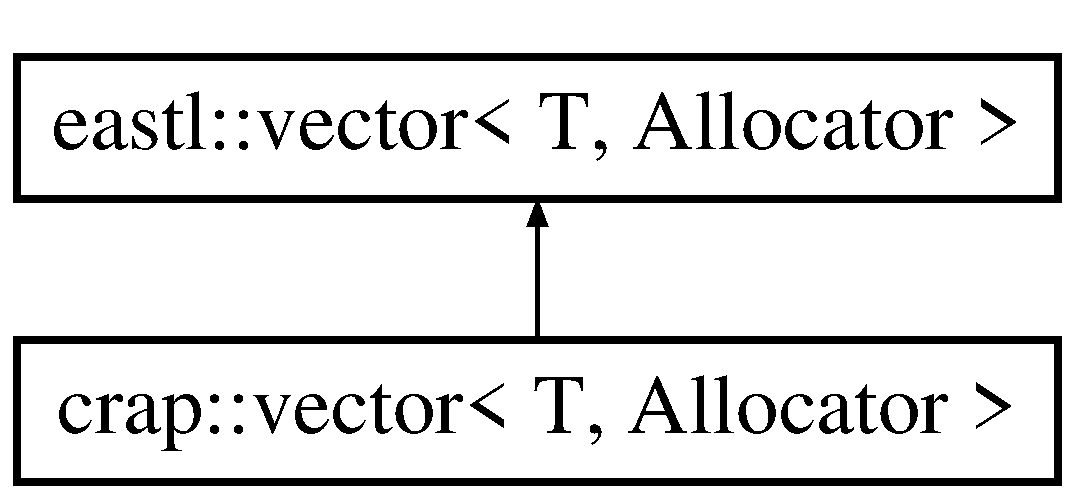
\includegraphics[height=2.000000cm]{classcrap_1_1vector}
\end{center}
\end{figure}


The documentation for this class was generated from the following file\-:\begin{DoxyCompactItemize}
\item 
/mnt/windows/data/\-Programmierung/\-C\-R\-A\-P/src/crap/container/\hyperlink{vector_8h}{vector.\-h}\end{DoxyCompactItemize}

\hypertarget{structcrap_1_1zero}{\section{crap\-:\-:zero$<$ T $>$ Struct Template Reference}
\label{structcrap_1_1zero}\index{crap\-::zero$<$ T $>$@{crap\-::zero$<$ T $>$}}
}


{\ttfamily \#include $<$zero.\-h$>$}

\subsection*{Static Public Attributes}
\begin{DoxyCompactItemize}
\item 
static const T \hyperlink{structcrap_1_1zero_adbf136ea6f7260ed699f6cbbb3a9ea46}{V\-A\-L\-U\-E} = 0
\end{DoxyCompactItemize}


\subsection{Member Data Documentation}
\hypertarget{structcrap_1_1zero_adbf136ea6f7260ed699f6cbbb3a9ea46}{\index{crap\-::zero@{crap\-::zero}!V\-A\-L\-U\-E@{V\-A\-L\-U\-E}}
\index{V\-A\-L\-U\-E@{V\-A\-L\-U\-E}!crap::zero@{crap\-::zero}}
\subsubsection[{V\-A\-L\-U\-E}]{\setlength{\rightskip}{0pt plus 5cm}template$<$typename T $>$ const T {\bf crap\-::zero}$<$ T $>$\-::V\-A\-L\-U\-E = 0\hspace{0.3cm}{\ttfamily [static]}}}\label{structcrap_1_1zero_adbf136ea6f7260ed699f6cbbb3a9ea46}


The documentation for this struct was generated from the following file\-:\begin{DoxyCompactItemize}
\item 
/mnt/windows/data/\-Programmierung/\-C\-R\-A\-P/src/crap/control/\hyperlink{zero_8h}{zero.\-h}\end{DoxyCompactItemize}

\hypertarget{structcrap_1_1zero_3_01f32_01_4}{\section{crap\-:\-:zero$<$ f32 $>$ Struct Template Reference}
\label{structcrap_1_1zero_3_01f32_01_4}\index{crap\-::zero$<$ f32 $>$@{crap\-::zero$<$ f32 $>$}}
}


{\ttfamily \#include $<$zero.\-h$>$}

\subsection*{Static Public Attributes}
\begin{DoxyCompactItemize}
\item 
static const \hyperlink{types_8h_a154db6eda6a99565cb060a1da4b4c930}{f32} \hyperlink{structcrap_1_1zero_3_01f32_01_4_a8f273005ab22247cb70022adac98953e}{V\-A\-L\-U\-E} = 0.\-0f
\begin{DoxyCompactList}\small\item\em \begin{DoxyCopyright}{Copyright}
Copyright (c) 2012 Steffen Kopany 
\end{DoxyCopyright}
\end{DoxyCompactList}\end{DoxyCompactItemize}


\subsection{Member Data Documentation}
\hypertarget{structcrap_1_1zero_3_01f32_01_4_a8f273005ab22247cb70022adac98953e}{\index{crap\-::zero$<$ f32 $>$@{crap\-::zero$<$ f32 $>$}!V\-A\-L\-U\-E@{V\-A\-L\-U\-E}}
\index{V\-A\-L\-U\-E@{V\-A\-L\-U\-E}!crap::zero< f32 >@{crap\-::zero$<$ f32 $>$}}
\subsubsection[{V\-A\-L\-U\-E}]{\setlength{\rightskip}{0pt plus 5cm}const {\bf f32} {\bf crap\-::zero}$<$ {\bf f32} $>$\-::V\-A\-L\-U\-E = 0.\-0f\hspace{0.3cm}{\ttfamily [static]}}}\label{structcrap_1_1zero_3_01f32_01_4_a8f273005ab22247cb70022adac98953e}


\begin{DoxyCopyright}{Copyright}
Copyright (c) 2012 Steffen Kopany 
\end{DoxyCopyright}


\begin{DoxyAuthor}{Author}
Steffen Kopany \href{mailto:steffen@kopany.at}{\tt steffen@kopany.\-at}Provides correct zero value 
\end{DoxyAuthor}
\begin{DoxyVersion}{Version}
scratch 
\end{DoxyVersion}


The documentation for this struct was generated from the following files\-:\begin{DoxyCompactItemize}
\item 
/mnt/windows/data/\-Programmierung/\-C\-R\-A\-P/src/crap/control/\hyperlink{zero_8h}{zero.\-h}\item 
/mnt/windows/data/\-Programmierung/\-C\-R\-A\-P/src/crap/control/\hyperlink{zero_8cpp}{zero.\-cpp}\end{DoxyCompactItemize}

\hypertarget{structcrap_1_1zero_3_01f64_01_4}{\section{crap\-:\-:zero$<$ f64 $>$ Struct Template Reference}
\label{structcrap_1_1zero_3_01f64_01_4}\index{crap\-::zero$<$ f64 $>$@{crap\-::zero$<$ f64 $>$}}
}


{\ttfamily \#include $<$zero.\-h$>$}

\subsection*{Static Public Attributes}
\begin{DoxyCompactItemize}
\item 
static const \hyperlink{types_8h_a76c9f53497f766e57b184bc8a93ab73f}{f64} \hyperlink{structcrap_1_1zero_3_01f64_01_4_a6467fb22f2cf48e955ddde385f23fac2}{V\-A\-L\-U\-E} = 0.\-0
\end{DoxyCompactItemize}


\subsection{Member Data Documentation}
\hypertarget{structcrap_1_1zero_3_01f64_01_4_a6467fb22f2cf48e955ddde385f23fac2}{\index{crap\-::zero$<$ f64 $>$@{crap\-::zero$<$ f64 $>$}!V\-A\-L\-U\-E@{V\-A\-L\-U\-E}}
\index{V\-A\-L\-U\-E@{V\-A\-L\-U\-E}!crap::zero< f64 >@{crap\-::zero$<$ f64 $>$}}
\subsubsection[{V\-A\-L\-U\-E}]{\setlength{\rightskip}{0pt plus 5cm}const {\bf f64} {\bf crap\-::zero}$<$ {\bf f64} $>$\-::V\-A\-L\-U\-E = 0.\-0\hspace{0.3cm}{\ttfamily [static]}}}\label{structcrap_1_1zero_3_01f64_01_4_a6467fb22f2cf48e955ddde385f23fac2}


The documentation for this struct was generated from the following files\-:\begin{DoxyCompactItemize}
\item 
/mnt/windows/data/\-Programmierung/\-C\-R\-A\-P/src/crap/control/\hyperlink{zero_8h}{zero.\-h}\item 
/mnt/windows/data/\-Programmierung/\-C\-R\-A\-P/src/crap/control/\hyperlink{zero_8cpp}{zero.\-cpp}\end{DoxyCompactItemize}

\chapter{File Documentation}
\hypertarget{config_8h}{\section{/mnt/windows/data/\-Programmierung/\-C\-R\-A\-P/src/crap/config.h File Reference}
\label{config_8h}\index{/mnt/windows/data/\-Programmierung/\-C\-R\-A\-P/src/crap/config.\-h@{/mnt/windows/data/\-Programmierung/\-C\-R\-A\-P/src/crap/config.\-h}}
}
{\ttfamily \#include \char`\"{}config/platforms.\-h\char`\"{}}\\*
{\ttfamily \#include \char`\"{}config/processors.\-h\char`\"{}}\\*
{\ttfamily \#include \char`\"{}config/compilers.\-h\char`\"{}}\\*
{\ttfamily \#include \char`\"{}config/types.\-h\char`\"{}}\\*
{\ttfamily \#include \char`\"{}config/endianness.\-h\char`\"{}}\\*
{\ttfamily \#include \char`\"{}config/threading.\-h\char`\"{}}\\*
{\ttfamily \#include \char`\"{}config/memory.\-h\char`\"{}}\\*
{\ttfamily \#include \char`\"{}config/simd.\-h\char`\"{}}\\*
{\ttfamily \#include \char`\"{}config/math.\-h\char`\"{}}\\*
\subsection*{Macros}
\begin{DoxyCompactItemize}
\item 
\#define \hyperlink{config_8h_ab45459525147b913a68b90421e01677f}{C\-R\-A\-P\-\_\-\-C\-O\-N\-F\-I\-G\-\_\-\-H}
\begin{DoxyCompactList}\small\item\em \begin{DoxyCopyright}{Copyright}
Copyright (c) 2012 Steffen Kopany 
\end{DoxyCopyright}
\end{DoxyCompactList}\end{DoxyCompactItemize}


\subsection{Macro Definition Documentation}
\hypertarget{config_8h_ab45459525147b913a68b90421e01677f}{\index{config.\-h@{config.\-h}!C\-R\-A\-P\-\_\-\-C\-O\-N\-F\-I\-G\-\_\-\-H@{C\-R\-A\-P\-\_\-\-C\-O\-N\-F\-I\-G\-\_\-\-H}}
\index{C\-R\-A\-P\-\_\-\-C\-O\-N\-F\-I\-G\-\_\-\-H@{C\-R\-A\-P\-\_\-\-C\-O\-N\-F\-I\-G\-\_\-\-H}!config.h@{config.\-h}}
\subsubsection[{C\-R\-A\-P\-\_\-\-C\-O\-N\-F\-I\-G\-\_\-\-H}]{\setlength{\rightskip}{0pt plus 5cm}\#define C\-R\-A\-P\-\_\-\-C\-O\-N\-F\-I\-G\-\_\-\-H}}\label{config_8h_ab45459525147b913a68b90421e01677f}


\begin{DoxyCopyright}{Copyright}
Copyright (c) 2012 Steffen Kopany 
\end{DoxyCopyright}


\begin{DoxyAuthor}{Author}
Steffen Kopany \href{mailto:steffen@kopany.at}{\tt steffen@kopany.\-at}Collecting all config/$\ast$.h files 
\end{DoxyAuthor}
\begin{DoxyVersion}{Version}
scratch 
\end{DoxyVersion}

\hypertarget{compilers_8h}{\section{/mnt/windows/data/\-Programmierung/\-C\-R\-A\-P/src/crap/config/compilers.h File Reference}
\label{compilers_8h}\index{/mnt/windows/data/\-Programmierung/\-C\-R\-A\-P/src/crap/config/compilers.\-h@{/mnt/windows/data/\-Programmierung/\-C\-R\-A\-P/src/crap/config/compilers.\-h}}
}
\subsection*{Namespaces}
\begin{DoxyCompactItemize}
\item 
namespace \hyperlink{namespacecrap}{crap}
\begin{DoxyCompactList}\small\item\em \begin{DoxyCopyright}{Copyright}
Copyright (c) 2012 Steffen Kopany 
\end{DoxyCopyright}
\end{DoxyCompactList}\end{DoxyCompactItemize}
\subsection*{Macros}
\begin{DoxyCompactItemize}
\item 
\#define \hyperlink{compilers_8h_aaa33868ff1f4b9977357928ea089a405}{C\-R\-A\-P\-\_\-\-C\-O\-N\-F\-I\-G\-\_\-\-C\-O\-M\-P\-I\-L\-E\-R\-S\-\_\-\-H}
\begin{DoxyCompactList}\small\item\em \begin{DoxyCopyright}{Copyright}
Copyright (c) 2012 Steffen Kopany 
\end{DoxyCopyright}
\end{DoxyCompactList}\item 
\#define \hyperlink{compilers_8h_aa2f3ddb2c18b14ac78c4306b0f74c9f2}{C\-R\-A\-P\-\_\-\-C\-O\-M\-P\-I\-L\-E\-R\-\_\-\-U\-N\-K\-N\-O\-W\-N}
\item 
\#define \hyperlink{compilers_8h_a477b9dbf38102bec988ebb0b6beb19c3}{C\-R\-A\-P\-\_\-\-C\-O\-M\-P\-I\-L\-E\-R\-\_\-\-N\-A\-M\-E}~\char`\"{}Unknown\char`\"{}
\item 
\#define \hyperlink{compilers_8h_a5a40526b8d842e7ff731509998bb0f1c}{C\-R\-A\-P\-\_\-\-I\-N\-L\-I\-N\-E}
\item 
\#define \hyperlink{compilers_8h_ad5edcf4fb82e86ea9831abb472bf3e40}{C\-R\-A\-P\-\_\-\-C\-P\-P}
\item 
\#define \hyperlink{compilers_8h_a5dd91cccfe66c6ba2c35488cb1b7631f}{C\-R\-A\-P\-\_\-\-T\-E\-M\-P\-L\-A\-T\-E\-\_\-\-C\-O\-N\-S\-T\-\_\-\-F\-I\-X}
\end{DoxyCompactItemize}
\subsection*{Enumerations}
\begin{DoxyCompactItemize}
\item 
enum \hyperlink{namespacecrap_a1118686d0b1bada904e097ebb2799067}{crap\-::compiler\-\_\-type} \{ \\*
\hyperlink{namespacecrap_a1118686d0b1bada904e097ebb2799067a622d828c592f48409bcab1c21220d317}{crap\-::gcc}, 
\hyperlink{namespacecrap_a1118686d0b1bada904e097ebb2799067a78c36762f3b9c3455946cf3e3021879d}{crap\-::vc}, 
\hyperlink{namespacecrap_a1118686d0b1bada904e097ebb2799067aba75e81d00209e8acc8aa3b616a24beb}{crap\-::borland}, 
\hyperlink{namespacecrap_a1118686d0b1bada904e097ebb2799067a5eccccfad078ff77b5d6a625768aed79}{crap\-::intel}, 
\\*
\hyperlink{namespacecrap_a1118686d0b1bada904e097ebb2799067acc56888524d023c251551fc013114194}{crap\-::unknown\-\_\-compiler}
 \}
\end{DoxyCompactItemize}


\subsection{Macro Definition Documentation}
\hypertarget{compilers_8h_a477b9dbf38102bec988ebb0b6beb19c3}{\index{compilers.\-h@{compilers.\-h}!C\-R\-A\-P\-\_\-\-C\-O\-M\-P\-I\-L\-E\-R\-\_\-\-N\-A\-M\-E@{C\-R\-A\-P\-\_\-\-C\-O\-M\-P\-I\-L\-E\-R\-\_\-\-N\-A\-M\-E}}
\index{C\-R\-A\-P\-\_\-\-C\-O\-M\-P\-I\-L\-E\-R\-\_\-\-N\-A\-M\-E@{C\-R\-A\-P\-\_\-\-C\-O\-M\-P\-I\-L\-E\-R\-\_\-\-N\-A\-M\-E}!compilers.h@{compilers.\-h}}
\subsubsection[{C\-R\-A\-P\-\_\-\-C\-O\-M\-P\-I\-L\-E\-R\-\_\-\-N\-A\-M\-E}]{\setlength{\rightskip}{0pt plus 5cm}\#define C\-R\-A\-P\-\_\-\-C\-O\-M\-P\-I\-L\-E\-R\-\_\-\-N\-A\-M\-E~\char`\"{}Unknown\char`\"{}}}\label{compilers_8h_a477b9dbf38102bec988ebb0b6beb19c3}
\hypertarget{compilers_8h_aa2f3ddb2c18b14ac78c4306b0f74c9f2}{\index{compilers.\-h@{compilers.\-h}!C\-R\-A\-P\-\_\-\-C\-O\-M\-P\-I\-L\-E\-R\-\_\-\-U\-N\-K\-N\-O\-W\-N@{C\-R\-A\-P\-\_\-\-C\-O\-M\-P\-I\-L\-E\-R\-\_\-\-U\-N\-K\-N\-O\-W\-N}}
\index{C\-R\-A\-P\-\_\-\-C\-O\-M\-P\-I\-L\-E\-R\-\_\-\-U\-N\-K\-N\-O\-W\-N@{C\-R\-A\-P\-\_\-\-C\-O\-M\-P\-I\-L\-E\-R\-\_\-\-U\-N\-K\-N\-O\-W\-N}!compilers.h@{compilers.\-h}}
\subsubsection[{C\-R\-A\-P\-\_\-\-C\-O\-M\-P\-I\-L\-E\-R\-\_\-\-U\-N\-K\-N\-O\-W\-N}]{\setlength{\rightskip}{0pt plus 5cm}\#define C\-R\-A\-P\-\_\-\-C\-O\-M\-P\-I\-L\-E\-R\-\_\-\-U\-N\-K\-N\-O\-W\-N}}\label{compilers_8h_aa2f3ddb2c18b14ac78c4306b0f74c9f2}
\hypertarget{compilers_8h_aaa33868ff1f4b9977357928ea089a405}{\index{compilers.\-h@{compilers.\-h}!C\-R\-A\-P\-\_\-\-C\-O\-N\-F\-I\-G\-\_\-\-C\-O\-M\-P\-I\-L\-E\-R\-S\-\_\-\-H@{C\-R\-A\-P\-\_\-\-C\-O\-N\-F\-I\-G\-\_\-\-C\-O\-M\-P\-I\-L\-E\-R\-S\-\_\-\-H}}
\index{C\-R\-A\-P\-\_\-\-C\-O\-N\-F\-I\-G\-\_\-\-C\-O\-M\-P\-I\-L\-E\-R\-S\-\_\-\-H@{C\-R\-A\-P\-\_\-\-C\-O\-N\-F\-I\-G\-\_\-\-C\-O\-M\-P\-I\-L\-E\-R\-S\-\_\-\-H}!compilers.h@{compilers.\-h}}
\subsubsection[{C\-R\-A\-P\-\_\-\-C\-O\-N\-F\-I\-G\-\_\-\-C\-O\-M\-P\-I\-L\-E\-R\-S\-\_\-\-H}]{\setlength{\rightskip}{0pt plus 5cm}\#define C\-R\-A\-P\-\_\-\-C\-O\-N\-F\-I\-G\-\_\-\-C\-O\-M\-P\-I\-L\-E\-R\-S\-\_\-\-H}}\label{compilers_8h_aaa33868ff1f4b9977357928ea089a405}


\begin{DoxyCopyright}{Copyright}
Copyright (c) 2012 Steffen Kopany 
\end{DoxyCopyright}


\begin{DoxyAuthor}{Author}
Steffen Kopany \href{mailto:steffen@kopany.at}{\tt steffen@kopany.\-at}Looking for compiler specific macros. 
\end{DoxyAuthor}
\begin{DoxyVersion}{Version}
scratch 
\end{DoxyVersion}
\hypertarget{compilers_8h_ad5edcf4fb82e86ea9831abb472bf3e40}{\index{compilers.\-h@{compilers.\-h}!C\-R\-A\-P\-\_\-\-C\-P\-P@{C\-R\-A\-P\-\_\-\-C\-P\-P}}
\index{C\-R\-A\-P\-\_\-\-C\-P\-P@{C\-R\-A\-P\-\_\-\-C\-P\-P}!compilers.h@{compilers.\-h}}
\subsubsection[{C\-R\-A\-P\-\_\-\-C\-P\-P}]{\setlength{\rightskip}{0pt plus 5cm}\#define C\-R\-A\-P\-\_\-\-C\-P\-P}}\label{compilers_8h_ad5edcf4fb82e86ea9831abb472bf3e40}
\hypertarget{compilers_8h_a5a40526b8d842e7ff731509998bb0f1c}{\index{compilers.\-h@{compilers.\-h}!C\-R\-A\-P\-\_\-\-I\-N\-L\-I\-N\-E@{C\-R\-A\-P\-\_\-\-I\-N\-L\-I\-N\-E}}
\index{C\-R\-A\-P\-\_\-\-I\-N\-L\-I\-N\-E@{C\-R\-A\-P\-\_\-\-I\-N\-L\-I\-N\-E}!compilers.h@{compilers.\-h}}
\subsubsection[{C\-R\-A\-P\-\_\-\-I\-N\-L\-I\-N\-E}]{\setlength{\rightskip}{0pt plus 5cm}\#define C\-R\-A\-P\-\_\-\-I\-N\-L\-I\-N\-E}}\label{compilers_8h_a5a40526b8d842e7ff731509998bb0f1c}
\hypertarget{compilers_8h_a5dd91cccfe66c6ba2c35488cb1b7631f}{\index{compilers.\-h@{compilers.\-h}!C\-R\-A\-P\-\_\-\-T\-E\-M\-P\-L\-A\-T\-E\-\_\-\-C\-O\-N\-S\-T\-\_\-\-F\-I\-X@{C\-R\-A\-P\-\_\-\-T\-E\-M\-P\-L\-A\-T\-E\-\_\-\-C\-O\-N\-S\-T\-\_\-\-F\-I\-X}}
\index{C\-R\-A\-P\-\_\-\-T\-E\-M\-P\-L\-A\-T\-E\-\_\-\-C\-O\-N\-S\-T\-\_\-\-F\-I\-X@{C\-R\-A\-P\-\_\-\-T\-E\-M\-P\-L\-A\-T\-E\-\_\-\-C\-O\-N\-S\-T\-\_\-\-F\-I\-X}!compilers.h@{compilers.\-h}}
\subsubsection[{C\-R\-A\-P\-\_\-\-T\-E\-M\-P\-L\-A\-T\-E\-\_\-\-C\-O\-N\-S\-T\-\_\-\-F\-I\-X}]{\setlength{\rightskip}{0pt plus 5cm}\#define C\-R\-A\-P\-\_\-\-T\-E\-M\-P\-L\-A\-T\-E\-\_\-\-C\-O\-N\-S\-T\-\_\-\-F\-I\-X}}\label{compilers_8h_a5dd91cccfe66c6ba2c35488cb1b7631f}

\hypertarget{endianness_8h}{\section{/mnt/windows/data/\-Programmierung/\-C\-R\-A\-P/src/crap/config/endianness.h File Reference}
\label{endianness_8h}\index{/mnt/windows/data/\-Programmierung/\-C\-R\-A\-P/src/crap/config/endianness.\-h@{/mnt/windows/data/\-Programmierung/\-C\-R\-A\-P/src/crap/config/endianness.\-h}}
}
{\ttfamily \#include \char`\"{}config/platforms.\-h\char`\"{}}\\*
{\ttfamily \#include \char`\"{}config/processors.\-h\char`\"{}}\\*
\subsection*{Macros}
\begin{DoxyCompactItemize}
\item 
\#define \hyperlink{endianness_8h_a6ab70f76fe037b88948de457e77f2875}{C\-R\-A\-P\-\_\-\-C\-O\-N\-F\-I\-G\-\_\-\-E\-N\-D\-I\-A\-N\-\_\-\-H}
\begin{DoxyCompactList}\small\item\em \begin{DoxyCopyright}{Copyright}
Copyright (c) 2012 Steffen Kopany 
\end{DoxyCopyright}
\end{DoxyCompactList}\item 
\#define \hyperlink{endianness_8h_ac1d9703e0f7c7dedb08e60ade9433f7c}{C\-R\-A\-P\-\_\-\-E\-N\-D\-I\-A\-N\-\_\-\-B\-I\-G}
\item 
\#define \hyperlink{endianness_8h_a7b04a4afd0319241617a17b6e4cee358}{C\-R\-A\-P\-\_\-\-E\-N\-D\-I\-A\-N\-\_\-\-I\-D}~1
\item 
\#define \hyperlink{endianness_8h_a04c6231b23364c14b8f8cbaf370f2194}{C\-R\-A\-P\-\_\-\-E\-N\-D\-I\-A\-N\-\_\-\-T\-Y\-P\-E}~\char`\"{}big\char`\"{}
\end{DoxyCompactItemize}


\subsection{Macro Definition Documentation}
\hypertarget{endianness_8h_a6ab70f76fe037b88948de457e77f2875}{\index{endianness.\-h@{endianness.\-h}!C\-R\-A\-P\-\_\-\-C\-O\-N\-F\-I\-G\-\_\-\-E\-N\-D\-I\-A\-N\-\_\-\-H@{C\-R\-A\-P\-\_\-\-C\-O\-N\-F\-I\-G\-\_\-\-E\-N\-D\-I\-A\-N\-\_\-\-H}}
\index{C\-R\-A\-P\-\_\-\-C\-O\-N\-F\-I\-G\-\_\-\-E\-N\-D\-I\-A\-N\-\_\-\-H@{C\-R\-A\-P\-\_\-\-C\-O\-N\-F\-I\-G\-\_\-\-E\-N\-D\-I\-A\-N\-\_\-\-H}!endianness.h@{endianness.\-h}}
\subsubsection[{C\-R\-A\-P\-\_\-\-C\-O\-N\-F\-I\-G\-\_\-\-E\-N\-D\-I\-A\-N\-\_\-\-H}]{\setlength{\rightskip}{0pt plus 5cm}\#define C\-R\-A\-P\-\_\-\-C\-O\-N\-F\-I\-G\-\_\-\-E\-N\-D\-I\-A\-N\-\_\-\-H}}\label{endianness_8h_a6ab70f76fe037b88948de457e77f2875}


\begin{DoxyCopyright}{Copyright}
Copyright (c) 2012 Steffen Kopany 
\end{DoxyCopyright}


\begin{DoxyAuthor}{Author}
Steffen Kopany \href{mailto:steffen@kopany.at}{\tt steffen@kopany.\-at}Checking / setting macros caring about 
\end{DoxyAuthor}
\begin{DoxyVersion}{Version}
scratch 
\end{DoxyVersion}
\hypertarget{endianness_8h_ac1d9703e0f7c7dedb08e60ade9433f7c}{\index{endianness.\-h@{endianness.\-h}!C\-R\-A\-P\-\_\-\-E\-N\-D\-I\-A\-N\-\_\-\-B\-I\-G@{C\-R\-A\-P\-\_\-\-E\-N\-D\-I\-A\-N\-\_\-\-B\-I\-G}}
\index{C\-R\-A\-P\-\_\-\-E\-N\-D\-I\-A\-N\-\_\-\-B\-I\-G@{C\-R\-A\-P\-\_\-\-E\-N\-D\-I\-A\-N\-\_\-\-B\-I\-G}!endianness.h@{endianness.\-h}}
\subsubsection[{C\-R\-A\-P\-\_\-\-E\-N\-D\-I\-A\-N\-\_\-\-B\-I\-G}]{\setlength{\rightskip}{0pt plus 5cm}\#define C\-R\-A\-P\-\_\-\-E\-N\-D\-I\-A\-N\-\_\-\-B\-I\-G}}\label{endianness_8h_ac1d9703e0f7c7dedb08e60ade9433f7c}
\hypertarget{endianness_8h_a7b04a4afd0319241617a17b6e4cee358}{\index{endianness.\-h@{endianness.\-h}!C\-R\-A\-P\-\_\-\-E\-N\-D\-I\-A\-N\-\_\-\-I\-D@{C\-R\-A\-P\-\_\-\-E\-N\-D\-I\-A\-N\-\_\-\-I\-D}}
\index{C\-R\-A\-P\-\_\-\-E\-N\-D\-I\-A\-N\-\_\-\-I\-D@{C\-R\-A\-P\-\_\-\-E\-N\-D\-I\-A\-N\-\_\-\-I\-D}!endianness.h@{endianness.\-h}}
\subsubsection[{C\-R\-A\-P\-\_\-\-E\-N\-D\-I\-A\-N\-\_\-\-I\-D}]{\setlength{\rightskip}{0pt plus 5cm}\#define C\-R\-A\-P\-\_\-\-E\-N\-D\-I\-A\-N\-\_\-\-I\-D~1}}\label{endianness_8h_a7b04a4afd0319241617a17b6e4cee358}
\hypertarget{endianness_8h_a04c6231b23364c14b8f8cbaf370f2194}{\index{endianness.\-h@{endianness.\-h}!C\-R\-A\-P\-\_\-\-E\-N\-D\-I\-A\-N\-\_\-\-T\-Y\-P\-E@{C\-R\-A\-P\-\_\-\-E\-N\-D\-I\-A\-N\-\_\-\-T\-Y\-P\-E}}
\index{C\-R\-A\-P\-\_\-\-E\-N\-D\-I\-A\-N\-\_\-\-T\-Y\-P\-E@{C\-R\-A\-P\-\_\-\-E\-N\-D\-I\-A\-N\-\_\-\-T\-Y\-P\-E}!endianness.h@{endianness.\-h}}
\subsubsection[{C\-R\-A\-P\-\_\-\-E\-N\-D\-I\-A\-N\-\_\-\-T\-Y\-P\-E}]{\setlength{\rightskip}{0pt plus 5cm}\#define C\-R\-A\-P\-\_\-\-E\-N\-D\-I\-A\-N\-\_\-\-T\-Y\-P\-E~\char`\"{}big\char`\"{}}}\label{endianness_8h_a04c6231b23364c14b8f8cbaf370f2194}

\hypertarget{config_2math_8h}{\section{/mnt/windows/data/\-Programmierung/\-C\-R\-A\-P/src/crap/config/math.h File Reference}
\label{config_2math_8h}\index{/mnt/windows/data/\-Programmierung/\-C\-R\-A\-P/src/crap/config/math.\-h@{/mnt/windows/data/\-Programmierung/\-C\-R\-A\-P/src/crap/config/math.\-h}}
}
\subsection*{Macros}
\begin{DoxyCompactItemize}
\item 
\#define \hyperlink{config_2math_8h_a0aafb1e19fdf40f22cf3921baee4a2bb}{C\-R\-A\-P\-\_\-\-C\-O\-N\-F\-I\-G\-\_\-\-M\-A\-T\-H\-\_\-\-H}
\begin{DoxyCompactList}\small\item\em \begin{DoxyCopyright}{Copyright}
Copyright (c) 2012 Steffen Kopany 
\end{DoxyCopyright}
\end{DoxyCompactList}\item 
\#define \hyperlink{config_2math_8h_a4f72eaf79226d0fca0407bf95eefabd1}{C\-R\-A\-P\-\_\-\-E}~2.\-71828182845904523536\-F
\item 
\#define \hyperlink{config_2math_8h_a3000f700b6003a9c2acd4c7dcaffd02c}{C\-R\-A\-P\-\_\-\-P\-I}~3.\-14159265358979323846\-F
\item 
\#define \hyperlink{config_2math_8h_ad3f80355dcfdeea3551a147b0f7c499c}{C\-R\-A\-P\-\_\-\-T\-W\-O\-\_\-\-P\-I}~6.\-28318530718958647692\-F
\item 
\#define \hyperlink{config_2math_8h_a0c6462e2ed29ddef88ed32b8f44c90e4}{C\-R\-A\-P\-\_\-\-P\-I\-\_\-\-H\-A\-L\-F}~1.\-57079632679489661923\-F
\item 
\#define \hyperlink{config_2math_8h_a44e825675df08543dbd4d7b83fe16e24}{C\-R\-A\-P\-\_\-\-P\-I\-\_\-\-Q\-U\-A\-T\-E\-R}~0.\-78539816339744830962\-F
\item 
\#define \hyperlink{config_2math_8h_af84466efa954ecf976b5409adb20c4d1}{C\-R\-A\-P\-\_\-1\-\_\-\-D\-I\-V\-\_\-\-P\-I}~0.\-31830988618379067154\-F
\item 
\#define \hyperlink{config_2math_8h_a39342e4ea1f7aabe9420821be6aa8f60}{C\-R\-A\-P\-\_\-2\-\_\-\-D\-I\-V\-\_\-\-P\-I}~0.\-63661977236758134308\-F
\item 
\#define \hyperlink{config_2math_8h_a7da3a989cbc9c5909693dfe671318c11}{C\-R\-A\-P\-\_\-\-L\-O\-G2\-E}~1.\-44269504088896340736\-F
\item 
\#define \hyperlink{config_2math_8h_a9326081f45a25ab17eddf061478d0670}{C\-R\-A\-P\-\_\-\-L\-O\-G10\-\_\-\-E}~0.\-43429448190325182765\-F
\item 
\#define \hyperlink{config_2math_8h_ad7b4cb504cfd34ccec4569a074e74e85}{C\-R\-A\-P\-\_\-\-L\-N\-\_\-2}~0.\-69314718055994530942\-F
\item 
\#define \hyperlink{config_2math_8h_a728b5a4cfd2a944727ad0cf10fbf6ee1}{C\-R\-A\-P\-\_\-\-L\-N\-\_\-10}~2.\-30258509299404568402\-F
\item 
\#define \hyperlink{config_2math_8h_af10c30d33a4247bfc1af650bfdb6007d}{C\-R\-A\-P\-\_\-2\-\_\-\-D\-I\-V\-\_\-\-S\-Q\-R\-T\-\_\-\-P\-I}~1.\-12837916709551257390\-F
\item 
\#define \hyperlink{config_2math_8h_ab09d052f8c0e34f744f23aff490a6b16}{C\-R\-A\-P\-\_\-\-S\-Q\-R\-T\-\_\-2}~1.\-41421356237309504880\-F
\item 
\#define \hyperlink{config_2math_8h_a91b1da43b1b2ee6732da8cac7b2481a9}{C\-R\-A\-P\-\_\-\-S\-Q\-R\-T\-\_\-3}~1.\-73205080756887729353\-F
\item 
\#define \hyperlink{config_2math_8h_aee69f425f81735338588c8bb96e283b9}{C\-R\-A\-P\-\_\-\-S\-Q\-R\-T\-\_\-1\-\_\-\-D\-I\-V\-\_\-2}~0.\-70710678118654752440\-F
\item 
\#define \hyperlink{config_2math_8h_a2751bfea0450621906439eeca068dd45}{C\-R\-A\-P\-\_\-\-S\-Q\-R\-T\-\_\-1\-\_\-\-D\-I\-V\-\_\-3}~0.\-57735027955204221151\-F
\item 
\#define \hyperlink{config_2math_8h_a32dc1f23fd6ba0538f3a12c1b85fc918}{C\-R\-A\-P\-\_\-\-S\-Q\-R\-T\-\_\-\-P\-I}~9.\-86960440108935861883\-F
\item 
\#define \hyperlink{config_2math_8h_a572e05e43d246b10bc87b85ce8890801}{C\-R\-A\-P\-\_\-\-D\-E\-G\-\_\-\-T\-O\-\_\-\-R\-A\-D}~0.\-01745329238\-F
\item 
\#define \hyperlink{config_2math_8h_ab2d0437aacd830dddffc2a092794f187}{C\-R\-A\-P\-\_\-\-R\-A\-D\-\_\-\-T\-O\-\_\-\-D\-E\-G}~57.\-295779513\-F
\item 
\#define \hyperlink{config_2math_8h_a32079c918acb1ea6c588abe599dd952c}{C\-R\-A\-P\-\_\-\-E\-P\-S\-I\-L\-O\-N}~1\-E-\/5\-F
\end{DoxyCompactItemize}


\subsection{Macro Definition Documentation}
\hypertarget{config_2math_8h_af84466efa954ecf976b5409adb20c4d1}{\index{config/math.\-h@{config/math.\-h}!C\-R\-A\-P\-\_\-1\-\_\-\-D\-I\-V\-\_\-\-P\-I@{C\-R\-A\-P\-\_\-1\-\_\-\-D\-I\-V\-\_\-\-P\-I}}
\index{C\-R\-A\-P\-\_\-1\-\_\-\-D\-I\-V\-\_\-\-P\-I@{C\-R\-A\-P\-\_\-1\-\_\-\-D\-I\-V\-\_\-\-P\-I}!config/math.h@{config/math.\-h}}
\subsubsection[{C\-R\-A\-P\-\_\-1\-\_\-\-D\-I\-V\-\_\-\-P\-I}]{\setlength{\rightskip}{0pt plus 5cm}\#define C\-R\-A\-P\-\_\-1\-\_\-\-D\-I\-V\-\_\-\-P\-I~0.\-31830988618379067154\-F}}\label{config_2math_8h_af84466efa954ecf976b5409adb20c4d1}
\hypertarget{config_2math_8h_a39342e4ea1f7aabe9420821be6aa8f60}{\index{config/math.\-h@{config/math.\-h}!C\-R\-A\-P\-\_\-2\-\_\-\-D\-I\-V\-\_\-\-P\-I@{C\-R\-A\-P\-\_\-2\-\_\-\-D\-I\-V\-\_\-\-P\-I}}
\index{C\-R\-A\-P\-\_\-2\-\_\-\-D\-I\-V\-\_\-\-P\-I@{C\-R\-A\-P\-\_\-2\-\_\-\-D\-I\-V\-\_\-\-P\-I}!config/math.h@{config/math.\-h}}
\subsubsection[{C\-R\-A\-P\-\_\-2\-\_\-\-D\-I\-V\-\_\-\-P\-I}]{\setlength{\rightskip}{0pt plus 5cm}\#define C\-R\-A\-P\-\_\-2\-\_\-\-D\-I\-V\-\_\-\-P\-I~0.\-63661977236758134308\-F}}\label{config_2math_8h_a39342e4ea1f7aabe9420821be6aa8f60}
\hypertarget{config_2math_8h_af10c30d33a4247bfc1af650bfdb6007d}{\index{config/math.\-h@{config/math.\-h}!C\-R\-A\-P\-\_\-2\-\_\-\-D\-I\-V\-\_\-\-S\-Q\-R\-T\-\_\-\-P\-I@{C\-R\-A\-P\-\_\-2\-\_\-\-D\-I\-V\-\_\-\-S\-Q\-R\-T\-\_\-\-P\-I}}
\index{C\-R\-A\-P\-\_\-2\-\_\-\-D\-I\-V\-\_\-\-S\-Q\-R\-T\-\_\-\-P\-I@{C\-R\-A\-P\-\_\-2\-\_\-\-D\-I\-V\-\_\-\-S\-Q\-R\-T\-\_\-\-P\-I}!config/math.h@{config/math.\-h}}
\subsubsection[{C\-R\-A\-P\-\_\-2\-\_\-\-D\-I\-V\-\_\-\-S\-Q\-R\-T\-\_\-\-P\-I}]{\setlength{\rightskip}{0pt plus 5cm}\#define C\-R\-A\-P\-\_\-2\-\_\-\-D\-I\-V\-\_\-\-S\-Q\-R\-T\-\_\-\-P\-I~1.\-12837916709551257390\-F}}\label{config_2math_8h_af10c30d33a4247bfc1af650bfdb6007d}
\hypertarget{config_2math_8h_a0aafb1e19fdf40f22cf3921baee4a2bb}{\index{config/math.\-h@{config/math.\-h}!C\-R\-A\-P\-\_\-\-C\-O\-N\-F\-I\-G\-\_\-\-M\-A\-T\-H\-\_\-\-H@{C\-R\-A\-P\-\_\-\-C\-O\-N\-F\-I\-G\-\_\-\-M\-A\-T\-H\-\_\-\-H}}
\index{C\-R\-A\-P\-\_\-\-C\-O\-N\-F\-I\-G\-\_\-\-M\-A\-T\-H\-\_\-\-H@{C\-R\-A\-P\-\_\-\-C\-O\-N\-F\-I\-G\-\_\-\-M\-A\-T\-H\-\_\-\-H}!config/math.h@{config/math.\-h}}
\subsubsection[{C\-R\-A\-P\-\_\-\-C\-O\-N\-F\-I\-G\-\_\-\-M\-A\-T\-H\-\_\-\-H}]{\setlength{\rightskip}{0pt plus 5cm}\#define C\-R\-A\-P\-\_\-\-C\-O\-N\-F\-I\-G\-\_\-\-M\-A\-T\-H\-\_\-\-H}}\label{config_2math_8h_a0aafb1e19fdf40f22cf3921baee4a2bb}


\begin{DoxyCopyright}{Copyright}
Copyright (c) 2012 Steffen Kopany 
\end{DoxyCopyright}


\begin{DoxyAuthor}{Author}
Steffen Kopany \href{mailto:steffen@kopany.at}{\tt steffen@kopany.\-at}Defines for math (constant values) 
\end{DoxyAuthor}
\begin{DoxyVersion}{Version}
scratch 
\end{DoxyVersion}
\hypertarget{config_2math_8h_a572e05e43d246b10bc87b85ce8890801}{\index{config/math.\-h@{config/math.\-h}!C\-R\-A\-P\-\_\-\-D\-E\-G\-\_\-\-T\-O\-\_\-\-R\-A\-D@{C\-R\-A\-P\-\_\-\-D\-E\-G\-\_\-\-T\-O\-\_\-\-R\-A\-D}}
\index{C\-R\-A\-P\-\_\-\-D\-E\-G\-\_\-\-T\-O\-\_\-\-R\-A\-D@{C\-R\-A\-P\-\_\-\-D\-E\-G\-\_\-\-T\-O\-\_\-\-R\-A\-D}!config/math.h@{config/math.\-h}}
\subsubsection[{C\-R\-A\-P\-\_\-\-D\-E\-G\-\_\-\-T\-O\-\_\-\-R\-A\-D}]{\setlength{\rightskip}{0pt plus 5cm}\#define C\-R\-A\-P\-\_\-\-D\-E\-G\-\_\-\-T\-O\-\_\-\-R\-A\-D~0.\-01745329238\-F}}\label{config_2math_8h_a572e05e43d246b10bc87b85ce8890801}
\hypertarget{config_2math_8h_a4f72eaf79226d0fca0407bf95eefabd1}{\index{config/math.\-h@{config/math.\-h}!C\-R\-A\-P\-\_\-\-E@{C\-R\-A\-P\-\_\-\-E}}
\index{C\-R\-A\-P\-\_\-\-E@{C\-R\-A\-P\-\_\-\-E}!config/math.h@{config/math.\-h}}
\subsubsection[{C\-R\-A\-P\-\_\-\-E}]{\setlength{\rightskip}{0pt plus 5cm}\#define C\-R\-A\-P\-\_\-\-E~2.\-71828182845904523536\-F}}\label{config_2math_8h_a4f72eaf79226d0fca0407bf95eefabd1}
\hypertarget{config_2math_8h_a32079c918acb1ea6c588abe599dd952c}{\index{config/math.\-h@{config/math.\-h}!C\-R\-A\-P\-\_\-\-E\-P\-S\-I\-L\-O\-N@{C\-R\-A\-P\-\_\-\-E\-P\-S\-I\-L\-O\-N}}
\index{C\-R\-A\-P\-\_\-\-E\-P\-S\-I\-L\-O\-N@{C\-R\-A\-P\-\_\-\-E\-P\-S\-I\-L\-O\-N}!config/math.h@{config/math.\-h}}
\subsubsection[{C\-R\-A\-P\-\_\-\-E\-P\-S\-I\-L\-O\-N}]{\setlength{\rightskip}{0pt plus 5cm}\#define C\-R\-A\-P\-\_\-\-E\-P\-S\-I\-L\-O\-N~1\-E-\/5\-F}}\label{config_2math_8h_a32079c918acb1ea6c588abe599dd952c}
\hypertarget{config_2math_8h_a728b5a4cfd2a944727ad0cf10fbf6ee1}{\index{config/math.\-h@{config/math.\-h}!C\-R\-A\-P\-\_\-\-L\-N\-\_\-10@{C\-R\-A\-P\-\_\-\-L\-N\-\_\-10}}
\index{C\-R\-A\-P\-\_\-\-L\-N\-\_\-10@{C\-R\-A\-P\-\_\-\-L\-N\-\_\-10}!config/math.h@{config/math.\-h}}
\subsubsection[{C\-R\-A\-P\-\_\-\-L\-N\-\_\-10}]{\setlength{\rightskip}{0pt plus 5cm}\#define C\-R\-A\-P\-\_\-\-L\-N\-\_\-10~2.\-30258509299404568402\-F}}\label{config_2math_8h_a728b5a4cfd2a944727ad0cf10fbf6ee1}
\hypertarget{config_2math_8h_ad7b4cb504cfd34ccec4569a074e74e85}{\index{config/math.\-h@{config/math.\-h}!C\-R\-A\-P\-\_\-\-L\-N\-\_\-2@{C\-R\-A\-P\-\_\-\-L\-N\-\_\-2}}
\index{C\-R\-A\-P\-\_\-\-L\-N\-\_\-2@{C\-R\-A\-P\-\_\-\-L\-N\-\_\-2}!config/math.h@{config/math.\-h}}
\subsubsection[{C\-R\-A\-P\-\_\-\-L\-N\-\_\-2}]{\setlength{\rightskip}{0pt plus 5cm}\#define C\-R\-A\-P\-\_\-\-L\-N\-\_\-2~0.\-69314718055994530942\-F}}\label{config_2math_8h_ad7b4cb504cfd34ccec4569a074e74e85}
\hypertarget{config_2math_8h_a9326081f45a25ab17eddf061478d0670}{\index{config/math.\-h@{config/math.\-h}!C\-R\-A\-P\-\_\-\-L\-O\-G10\-\_\-\-E@{C\-R\-A\-P\-\_\-\-L\-O\-G10\-\_\-\-E}}
\index{C\-R\-A\-P\-\_\-\-L\-O\-G10\-\_\-\-E@{C\-R\-A\-P\-\_\-\-L\-O\-G10\-\_\-\-E}!config/math.h@{config/math.\-h}}
\subsubsection[{C\-R\-A\-P\-\_\-\-L\-O\-G10\-\_\-\-E}]{\setlength{\rightskip}{0pt plus 5cm}\#define C\-R\-A\-P\-\_\-\-L\-O\-G10\-\_\-\-E~0.\-43429448190325182765\-F}}\label{config_2math_8h_a9326081f45a25ab17eddf061478d0670}
\hypertarget{config_2math_8h_a7da3a989cbc9c5909693dfe671318c11}{\index{config/math.\-h@{config/math.\-h}!C\-R\-A\-P\-\_\-\-L\-O\-G2\-E@{C\-R\-A\-P\-\_\-\-L\-O\-G2\-E}}
\index{C\-R\-A\-P\-\_\-\-L\-O\-G2\-E@{C\-R\-A\-P\-\_\-\-L\-O\-G2\-E}!config/math.h@{config/math.\-h}}
\subsubsection[{C\-R\-A\-P\-\_\-\-L\-O\-G2\-E}]{\setlength{\rightskip}{0pt plus 5cm}\#define C\-R\-A\-P\-\_\-\-L\-O\-G2\-E~1.\-44269504088896340736\-F}}\label{config_2math_8h_a7da3a989cbc9c5909693dfe671318c11}
\hypertarget{config_2math_8h_a3000f700b6003a9c2acd4c7dcaffd02c}{\index{config/math.\-h@{config/math.\-h}!C\-R\-A\-P\-\_\-\-P\-I@{C\-R\-A\-P\-\_\-\-P\-I}}
\index{C\-R\-A\-P\-\_\-\-P\-I@{C\-R\-A\-P\-\_\-\-P\-I}!config/math.h@{config/math.\-h}}
\subsubsection[{C\-R\-A\-P\-\_\-\-P\-I}]{\setlength{\rightskip}{0pt plus 5cm}\#define C\-R\-A\-P\-\_\-\-P\-I~3.\-14159265358979323846\-F}}\label{config_2math_8h_a3000f700b6003a9c2acd4c7dcaffd02c}
\hypertarget{config_2math_8h_a0c6462e2ed29ddef88ed32b8f44c90e4}{\index{config/math.\-h@{config/math.\-h}!C\-R\-A\-P\-\_\-\-P\-I\-\_\-\-H\-A\-L\-F@{C\-R\-A\-P\-\_\-\-P\-I\-\_\-\-H\-A\-L\-F}}
\index{C\-R\-A\-P\-\_\-\-P\-I\-\_\-\-H\-A\-L\-F@{C\-R\-A\-P\-\_\-\-P\-I\-\_\-\-H\-A\-L\-F}!config/math.h@{config/math.\-h}}
\subsubsection[{C\-R\-A\-P\-\_\-\-P\-I\-\_\-\-H\-A\-L\-F}]{\setlength{\rightskip}{0pt plus 5cm}\#define C\-R\-A\-P\-\_\-\-P\-I\-\_\-\-H\-A\-L\-F~1.\-57079632679489661923\-F}}\label{config_2math_8h_a0c6462e2ed29ddef88ed32b8f44c90e4}
\hypertarget{config_2math_8h_a44e825675df08543dbd4d7b83fe16e24}{\index{config/math.\-h@{config/math.\-h}!C\-R\-A\-P\-\_\-\-P\-I\-\_\-\-Q\-U\-A\-T\-E\-R@{C\-R\-A\-P\-\_\-\-P\-I\-\_\-\-Q\-U\-A\-T\-E\-R}}
\index{C\-R\-A\-P\-\_\-\-P\-I\-\_\-\-Q\-U\-A\-T\-E\-R@{C\-R\-A\-P\-\_\-\-P\-I\-\_\-\-Q\-U\-A\-T\-E\-R}!config/math.h@{config/math.\-h}}
\subsubsection[{C\-R\-A\-P\-\_\-\-P\-I\-\_\-\-Q\-U\-A\-T\-E\-R}]{\setlength{\rightskip}{0pt plus 5cm}\#define C\-R\-A\-P\-\_\-\-P\-I\-\_\-\-Q\-U\-A\-T\-E\-R~0.\-78539816339744830962\-F}}\label{config_2math_8h_a44e825675df08543dbd4d7b83fe16e24}
\hypertarget{config_2math_8h_ab2d0437aacd830dddffc2a092794f187}{\index{config/math.\-h@{config/math.\-h}!C\-R\-A\-P\-\_\-\-R\-A\-D\-\_\-\-T\-O\-\_\-\-D\-E\-G@{C\-R\-A\-P\-\_\-\-R\-A\-D\-\_\-\-T\-O\-\_\-\-D\-E\-G}}
\index{C\-R\-A\-P\-\_\-\-R\-A\-D\-\_\-\-T\-O\-\_\-\-D\-E\-G@{C\-R\-A\-P\-\_\-\-R\-A\-D\-\_\-\-T\-O\-\_\-\-D\-E\-G}!config/math.h@{config/math.\-h}}
\subsubsection[{C\-R\-A\-P\-\_\-\-R\-A\-D\-\_\-\-T\-O\-\_\-\-D\-E\-G}]{\setlength{\rightskip}{0pt plus 5cm}\#define C\-R\-A\-P\-\_\-\-R\-A\-D\-\_\-\-T\-O\-\_\-\-D\-E\-G~57.\-295779513\-F}}\label{config_2math_8h_ab2d0437aacd830dddffc2a092794f187}
\hypertarget{config_2math_8h_aee69f425f81735338588c8bb96e283b9}{\index{config/math.\-h@{config/math.\-h}!C\-R\-A\-P\-\_\-\-S\-Q\-R\-T\-\_\-1\-\_\-\-D\-I\-V\-\_\-2@{C\-R\-A\-P\-\_\-\-S\-Q\-R\-T\-\_\-1\-\_\-\-D\-I\-V\-\_\-2}}
\index{C\-R\-A\-P\-\_\-\-S\-Q\-R\-T\-\_\-1\-\_\-\-D\-I\-V\-\_\-2@{C\-R\-A\-P\-\_\-\-S\-Q\-R\-T\-\_\-1\-\_\-\-D\-I\-V\-\_\-2}!config/math.h@{config/math.\-h}}
\subsubsection[{C\-R\-A\-P\-\_\-\-S\-Q\-R\-T\-\_\-1\-\_\-\-D\-I\-V\-\_\-2}]{\setlength{\rightskip}{0pt plus 5cm}\#define C\-R\-A\-P\-\_\-\-S\-Q\-R\-T\-\_\-1\-\_\-\-D\-I\-V\-\_\-2~0.\-70710678118654752440\-F}}\label{config_2math_8h_aee69f425f81735338588c8bb96e283b9}
\hypertarget{config_2math_8h_a2751bfea0450621906439eeca068dd45}{\index{config/math.\-h@{config/math.\-h}!C\-R\-A\-P\-\_\-\-S\-Q\-R\-T\-\_\-1\-\_\-\-D\-I\-V\-\_\-3@{C\-R\-A\-P\-\_\-\-S\-Q\-R\-T\-\_\-1\-\_\-\-D\-I\-V\-\_\-3}}
\index{C\-R\-A\-P\-\_\-\-S\-Q\-R\-T\-\_\-1\-\_\-\-D\-I\-V\-\_\-3@{C\-R\-A\-P\-\_\-\-S\-Q\-R\-T\-\_\-1\-\_\-\-D\-I\-V\-\_\-3}!config/math.h@{config/math.\-h}}
\subsubsection[{C\-R\-A\-P\-\_\-\-S\-Q\-R\-T\-\_\-1\-\_\-\-D\-I\-V\-\_\-3}]{\setlength{\rightskip}{0pt plus 5cm}\#define C\-R\-A\-P\-\_\-\-S\-Q\-R\-T\-\_\-1\-\_\-\-D\-I\-V\-\_\-3~0.\-57735027955204221151\-F}}\label{config_2math_8h_a2751bfea0450621906439eeca068dd45}
\hypertarget{config_2math_8h_ab09d052f8c0e34f744f23aff490a6b16}{\index{config/math.\-h@{config/math.\-h}!C\-R\-A\-P\-\_\-\-S\-Q\-R\-T\-\_\-2@{C\-R\-A\-P\-\_\-\-S\-Q\-R\-T\-\_\-2}}
\index{C\-R\-A\-P\-\_\-\-S\-Q\-R\-T\-\_\-2@{C\-R\-A\-P\-\_\-\-S\-Q\-R\-T\-\_\-2}!config/math.h@{config/math.\-h}}
\subsubsection[{C\-R\-A\-P\-\_\-\-S\-Q\-R\-T\-\_\-2}]{\setlength{\rightskip}{0pt plus 5cm}\#define C\-R\-A\-P\-\_\-\-S\-Q\-R\-T\-\_\-2~1.\-41421356237309504880\-F}}\label{config_2math_8h_ab09d052f8c0e34f744f23aff490a6b16}
\hypertarget{config_2math_8h_a91b1da43b1b2ee6732da8cac7b2481a9}{\index{config/math.\-h@{config/math.\-h}!C\-R\-A\-P\-\_\-\-S\-Q\-R\-T\-\_\-3@{C\-R\-A\-P\-\_\-\-S\-Q\-R\-T\-\_\-3}}
\index{C\-R\-A\-P\-\_\-\-S\-Q\-R\-T\-\_\-3@{C\-R\-A\-P\-\_\-\-S\-Q\-R\-T\-\_\-3}!config/math.h@{config/math.\-h}}
\subsubsection[{C\-R\-A\-P\-\_\-\-S\-Q\-R\-T\-\_\-3}]{\setlength{\rightskip}{0pt plus 5cm}\#define C\-R\-A\-P\-\_\-\-S\-Q\-R\-T\-\_\-3~1.\-73205080756887729353\-F}}\label{config_2math_8h_a91b1da43b1b2ee6732da8cac7b2481a9}
\hypertarget{config_2math_8h_a32dc1f23fd6ba0538f3a12c1b85fc918}{\index{config/math.\-h@{config/math.\-h}!C\-R\-A\-P\-\_\-\-S\-Q\-R\-T\-\_\-\-P\-I@{C\-R\-A\-P\-\_\-\-S\-Q\-R\-T\-\_\-\-P\-I}}
\index{C\-R\-A\-P\-\_\-\-S\-Q\-R\-T\-\_\-\-P\-I@{C\-R\-A\-P\-\_\-\-S\-Q\-R\-T\-\_\-\-P\-I}!config/math.h@{config/math.\-h}}
\subsubsection[{C\-R\-A\-P\-\_\-\-S\-Q\-R\-T\-\_\-\-P\-I}]{\setlength{\rightskip}{0pt plus 5cm}\#define C\-R\-A\-P\-\_\-\-S\-Q\-R\-T\-\_\-\-P\-I~9.\-86960440108935861883\-F}}\label{config_2math_8h_a32dc1f23fd6ba0538f3a12c1b85fc918}
\hypertarget{config_2math_8h_ad3f80355dcfdeea3551a147b0f7c499c}{\index{config/math.\-h@{config/math.\-h}!C\-R\-A\-P\-\_\-\-T\-W\-O\-\_\-\-P\-I@{C\-R\-A\-P\-\_\-\-T\-W\-O\-\_\-\-P\-I}}
\index{C\-R\-A\-P\-\_\-\-T\-W\-O\-\_\-\-P\-I@{C\-R\-A\-P\-\_\-\-T\-W\-O\-\_\-\-P\-I}!config/math.h@{config/math.\-h}}
\subsubsection[{C\-R\-A\-P\-\_\-\-T\-W\-O\-\_\-\-P\-I}]{\setlength{\rightskip}{0pt plus 5cm}\#define C\-R\-A\-P\-\_\-\-T\-W\-O\-\_\-\-P\-I~6.\-28318530718958647692\-F}}\label{config_2math_8h_ad3f80355dcfdeea3551a147b0f7c499c}

\hypertarget{math_2math_8h}{\section{/mnt/windows/data/\-Programmierung/\-C\-R\-A\-P/src/crap/math/math.h File Reference}
\label{math_2math_8h}\index{/mnt/windows/data/\-Programmierung/\-C\-R\-A\-P/src/crap/math/math.\-h@{/mnt/windows/data/\-Programmierung/\-C\-R\-A\-P/src/crap/math/math.\-h}}
}
{\ttfamily \#include \char`\"{}config/math.\-h\char`\"{}}\\*
\subsection*{Classes}
\begin{DoxyCompactItemize}
\item 
class \hyperlink{classcrap_1_1math}{crap\-::math}
\end{DoxyCompactItemize}
\subsection*{Namespaces}
\begin{DoxyCompactItemize}
\item 
namespace \hyperlink{namespacecrap}{crap}
\begin{DoxyCompactList}\small\item\em \begin{DoxyCopyright}{Copyright}
Copyright (c) 2012 Steffen Kopany 
\end{DoxyCopyright}
\end{DoxyCompactList}\end{DoxyCompactItemize}
\subsection*{Macros}
\begin{DoxyCompactItemize}
\item 
\#define \hyperlink{math_2math_8h_a41ff98e0b00d2702dafd40c98b193d2c}{C\-R\-A\-P\-\_\-\-M\-A\-T\-H\-\_\-\-M\-A\-T\-H\-\_\-\-H}
\begin{DoxyCompactList}\small\item\em \begin{DoxyCopyright}{Copyright}
Copyright (c) 2012 Steffen Kopany 
\end{DoxyCopyright}
\end{DoxyCompactList}\end{DoxyCompactItemize}


\subsection{Macro Definition Documentation}
\hypertarget{math_2math_8h_a41ff98e0b00d2702dafd40c98b193d2c}{\index{math/math.\-h@{math/math.\-h}!C\-R\-A\-P\-\_\-\-M\-A\-T\-H\-\_\-\-M\-A\-T\-H\-\_\-\-H@{C\-R\-A\-P\-\_\-\-M\-A\-T\-H\-\_\-\-M\-A\-T\-H\-\_\-\-H}}
\index{C\-R\-A\-P\-\_\-\-M\-A\-T\-H\-\_\-\-M\-A\-T\-H\-\_\-\-H@{C\-R\-A\-P\-\_\-\-M\-A\-T\-H\-\_\-\-M\-A\-T\-H\-\_\-\-H}!math/math.h@{math/math.\-h}}
\subsubsection[{C\-R\-A\-P\-\_\-\-M\-A\-T\-H\-\_\-\-M\-A\-T\-H\-\_\-\-H}]{\setlength{\rightskip}{0pt plus 5cm}\#define C\-R\-A\-P\-\_\-\-M\-A\-T\-H\-\_\-\-M\-A\-T\-H\-\_\-\-H}}\label{math_2math_8h_a41ff98e0b00d2702dafd40c98b193d2c}


\begin{DoxyCopyright}{Copyright}
Copyright (c) 2012 Steffen Kopany 
\end{DoxyCopyright}


\begin{DoxyAuthor}{Author}
Steffen Kopany \href{mailto:steffen@kopany.at}{\tt steffen@kopany.\-at}Math functions using approximation and 
\end{DoxyAuthor}
\begin{DoxyVersion}{Version}
scratch 
\end{DoxyVersion}

\hypertarget{memory_8h}{\section{/mnt/windows/data/\-Programmierung/\-C\-R\-A\-P/src/crap/config/memory.h File Reference}
\label{memory_8h}\index{/mnt/windows/data/\-Programmierung/\-C\-R\-A\-P/src/crap/config/memory.\-h@{/mnt/windows/data/\-Programmierung/\-C\-R\-A\-P/src/crap/config/memory.\-h}}
}
\subsection*{Macros}
\begin{DoxyCompactItemize}
\item 
\#define \hyperlink{memory_8h_a6c407a6448d36daabcaeba4416ea43a1}{C\-R\-A\-P\-\_\-\-C\-O\-N\-F\-I\-G\-\_\-\-M\-E\-M\-O\-R\-Y\-\_\-\-H}
\begin{DoxyCompactList}\small\item\em \begin{DoxyCopyright}{Copyright}
Copyright (c) 2012 Steffen Kopany 
\end{DoxyCopyright}
\end{DoxyCompactList}\item 
\#define \hyperlink{memory_8h_af5048811917a1bea9ae9ed34e17f64e3}{C\-R\-A\-P\-\_\-\-M\-E\-M\-O\-R\-Y\-\_\-\-M\-A\-N\-A\-G\-E\-R}
\item 
\#define \hyperlink{memory_8h_a2f03bc5b63031718649591fe736b77e6}{C\-R\-A\-P\-\_\-\-M\-E\-M\-O\-R\-Y\-\_\-\-T\-R\-A\-C\-K\-E\-R}
\item 
\#define \hyperlink{memory_8h_a76f5c5ecde940b058aa6fec1a7103d23}{C\-R\-A\-P\-\_\-\-G\-A\-R\-B\-A\-G\-E\-\_\-\-C\-O\-L\-L\-E\-C\-T\-O\-R}
\item 
\#define \hyperlink{memory_8h_a77aad550a67548322f09d6f455181f2d}{C\-R\-A\-P\-\_\-\-G\-C\-\_\-\-T\-I\-C\-K}~1000000
\end{DoxyCompactItemize}


\subsection{Macro Definition Documentation}
\hypertarget{memory_8h_a6c407a6448d36daabcaeba4416ea43a1}{\index{memory.\-h@{memory.\-h}!C\-R\-A\-P\-\_\-\-C\-O\-N\-F\-I\-G\-\_\-\-M\-E\-M\-O\-R\-Y\-\_\-\-H@{C\-R\-A\-P\-\_\-\-C\-O\-N\-F\-I\-G\-\_\-\-M\-E\-M\-O\-R\-Y\-\_\-\-H}}
\index{C\-R\-A\-P\-\_\-\-C\-O\-N\-F\-I\-G\-\_\-\-M\-E\-M\-O\-R\-Y\-\_\-\-H@{C\-R\-A\-P\-\_\-\-C\-O\-N\-F\-I\-G\-\_\-\-M\-E\-M\-O\-R\-Y\-\_\-\-H}!memory.h@{memory.\-h}}
\subsubsection[{C\-R\-A\-P\-\_\-\-C\-O\-N\-F\-I\-G\-\_\-\-M\-E\-M\-O\-R\-Y\-\_\-\-H}]{\setlength{\rightskip}{0pt plus 5cm}\#define C\-R\-A\-P\-\_\-\-C\-O\-N\-F\-I\-G\-\_\-\-M\-E\-M\-O\-R\-Y\-\_\-\-H}}\label{memory_8h_a6c407a6448d36daabcaeba4416ea43a1}


\begin{DoxyCopyright}{Copyright}
Copyright (c) 2012 Steffen Kopany 
\end{DoxyCopyright}


\begin{DoxyAuthor}{Author}
Steffen Kopany \href{mailto:steffen@kopany.at}{\tt steffen@kopany.\-at}Setting memory macros (depricated) 
\end{DoxyAuthor}
\begin{DoxyVersion}{Version}
scratch 
\end{DoxyVersion}
\hypertarget{memory_8h_a76f5c5ecde940b058aa6fec1a7103d23}{\index{memory.\-h@{memory.\-h}!C\-R\-A\-P\-\_\-\-G\-A\-R\-B\-A\-G\-E\-\_\-\-C\-O\-L\-L\-E\-C\-T\-O\-R@{C\-R\-A\-P\-\_\-\-G\-A\-R\-B\-A\-G\-E\-\_\-\-C\-O\-L\-L\-E\-C\-T\-O\-R}}
\index{C\-R\-A\-P\-\_\-\-G\-A\-R\-B\-A\-G\-E\-\_\-\-C\-O\-L\-L\-E\-C\-T\-O\-R@{C\-R\-A\-P\-\_\-\-G\-A\-R\-B\-A\-G\-E\-\_\-\-C\-O\-L\-L\-E\-C\-T\-O\-R}!memory.h@{memory.\-h}}
\subsubsection[{C\-R\-A\-P\-\_\-\-G\-A\-R\-B\-A\-G\-E\-\_\-\-C\-O\-L\-L\-E\-C\-T\-O\-R}]{\setlength{\rightskip}{0pt plus 5cm}\#define C\-R\-A\-P\-\_\-\-G\-A\-R\-B\-A\-G\-E\-\_\-\-C\-O\-L\-L\-E\-C\-T\-O\-R}}\label{memory_8h_a76f5c5ecde940b058aa6fec1a7103d23}
\hypertarget{memory_8h_a77aad550a67548322f09d6f455181f2d}{\index{memory.\-h@{memory.\-h}!C\-R\-A\-P\-\_\-\-G\-C\-\_\-\-T\-I\-C\-K@{C\-R\-A\-P\-\_\-\-G\-C\-\_\-\-T\-I\-C\-K}}
\index{C\-R\-A\-P\-\_\-\-G\-C\-\_\-\-T\-I\-C\-K@{C\-R\-A\-P\-\_\-\-G\-C\-\_\-\-T\-I\-C\-K}!memory.h@{memory.\-h}}
\subsubsection[{C\-R\-A\-P\-\_\-\-G\-C\-\_\-\-T\-I\-C\-K}]{\setlength{\rightskip}{0pt plus 5cm}\#define C\-R\-A\-P\-\_\-\-G\-C\-\_\-\-T\-I\-C\-K~1000000}}\label{memory_8h_a77aad550a67548322f09d6f455181f2d}
\hypertarget{memory_8h_af5048811917a1bea9ae9ed34e17f64e3}{\index{memory.\-h@{memory.\-h}!C\-R\-A\-P\-\_\-\-M\-E\-M\-O\-R\-Y\-\_\-\-M\-A\-N\-A\-G\-E\-R@{C\-R\-A\-P\-\_\-\-M\-E\-M\-O\-R\-Y\-\_\-\-M\-A\-N\-A\-G\-E\-R}}
\index{C\-R\-A\-P\-\_\-\-M\-E\-M\-O\-R\-Y\-\_\-\-M\-A\-N\-A\-G\-E\-R@{C\-R\-A\-P\-\_\-\-M\-E\-M\-O\-R\-Y\-\_\-\-M\-A\-N\-A\-G\-E\-R}!memory.h@{memory.\-h}}
\subsubsection[{C\-R\-A\-P\-\_\-\-M\-E\-M\-O\-R\-Y\-\_\-\-M\-A\-N\-A\-G\-E\-R}]{\setlength{\rightskip}{0pt plus 5cm}\#define C\-R\-A\-P\-\_\-\-M\-E\-M\-O\-R\-Y\-\_\-\-M\-A\-N\-A\-G\-E\-R}}\label{memory_8h_af5048811917a1bea9ae9ed34e17f64e3}
\hypertarget{memory_8h_a2f03bc5b63031718649591fe736b77e6}{\index{memory.\-h@{memory.\-h}!C\-R\-A\-P\-\_\-\-M\-E\-M\-O\-R\-Y\-\_\-\-T\-R\-A\-C\-K\-E\-R@{C\-R\-A\-P\-\_\-\-M\-E\-M\-O\-R\-Y\-\_\-\-T\-R\-A\-C\-K\-E\-R}}
\index{C\-R\-A\-P\-\_\-\-M\-E\-M\-O\-R\-Y\-\_\-\-T\-R\-A\-C\-K\-E\-R@{C\-R\-A\-P\-\_\-\-M\-E\-M\-O\-R\-Y\-\_\-\-T\-R\-A\-C\-K\-E\-R}!memory.h@{memory.\-h}}
\subsubsection[{C\-R\-A\-P\-\_\-\-M\-E\-M\-O\-R\-Y\-\_\-\-T\-R\-A\-C\-K\-E\-R}]{\setlength{\rightskip}{0pt plus 5cm}\#define C\-R\-A\-P\-\_\-\-M\-E\-M\-O\-R\-Y\-\_\-\-T\-R\-A\-C\-K\-E\-R}}\label{memory_8h_a2f03bc5b63031718649591fe736b77e6}

\hypertarget{platforms_8h}{\section{/mnt/windows/data/\-Programmierung/\-C\-R\-A\-P/src/crap/config/platforms.h File Reference}
\label{platforms_8h}\index{/mnt/windows/data/\-Programmierung/\-C\-R\-A\-P/src/crap/config/platforms.\-h@{/mnt/windows/data/\-Programmierung/\-C\-R\-A\-P/src/crap/config/platforms.\-h}}
}
\subsection*{Namespaces}
\begin{DoxyCompactItemize}
\item 
namespace \hyperlink{namespacecrap}{crap}
\begin{DoxyCompactList}\small\item\em \begin{DoxyCopyright}{Copyright}
Copyright (c) 2012 Steffen Kopany 
\end{DoxyCopyright}
\end{DoxyCompactList}\end{DoxyCompactItemize}
\subsection*{Macros}
\begin{DoxyCompactItemize}
\item 
\#define \hyperlink{platforms_8h_a2d850503adb9f506644ce4552cb1bfe6}{C\-R\-A\-P\-\_\-\-C\-O\-N\-F\-I\-G\-\_\-\-P\-L\-A\-T\-F\-O\-R\-M\-S\-\_\-\-H}
\begin{DoxyCompactList}\small\item\em \begin{DoxyCopyright}{Copyright}
Copyright (c) 2012 Steffen Kopany 
\end{DoxyCopyright}
\end{DoxyCompactList}\item 
\#define \hyperlink{platforms_8h_ae2d64b895cb8de27bc534c2f9cce9f78}{C\-R\-A\-P\-\_\-\-P\-L\-A\-T\-F\-O\-R\-M\-\_\-\-U\-N\-K\-N\-O\-W\-N}
\item 
\#define \hyperlink{platforms_8h_afe86fc088b0d61ec8c1ed2294754bea1}{C\-R\-A\-P\-\_\-\-P\-L\-A\-T\-F\-O\-R\-M\-\_\-\-N\-A\-M\-E}~\char`\"{}Unknown\char`\"{}
\end{DoxyCompactItemize}
\subsection*{Enumerations}
\begin{DoxyCompactItemize}
\item 
enum \hyperlink{namespacecrap_a3ef4fad3b9a9befc38e0602d9b8323fd}{crap\-::os} \{ \\*
\hyperlink{namespacecrap_a3ef4fad3b9a9befc38e0602d9b8323fda0c640784849b6df0f3331dd2496499fa}{crap\-::platform\-\_\-windows}, 
\hyperlink{namespacecrap_a3ef4fad3b9a9befc38e0602d9b8323fda638127da44361ae111082b4150307136}{crap\-::platform\-\_\-macintosh}, 
\hyperlink{namespacecrap_a3ef4fad3b9a9befc38e0602d9b8323fda93bda5d1a82014723b1efe5f053d4d0b}{crap\-::platform\-\_\-ios}, 
\hyperlink{namespacecrap_a3ef4fad3b9a9befc38e0602d9b8323fda23ed65cb4c48a5f5765ab5b8978fbcdc}{crap\-::platform\-\_\-linux}, 
\\*
\hyperlink{namespacecrap_a3ef4fad3b9a9befc38e0602d9b8323fdac7cf11bbf8c16dda98d0d756df1e2ea5}{crap\-::platform\-\_\-bsd}, 
\hyperlink{namespacecrap_a3ef4fad3b9a9befc38e0602d9b8323fda2d1d2b6838c3fe48cb6beaf3cb23ae23}{crap\-::platform\-\_\-unix}, 
\hyperlink{namespacecrap_a3ef4fad3b9a9befc38e0602d9b8323fda40a17798d2969201f9dbc4ffec789e91}{crap\-::platform\-\_\-unknown}
 \}
\end{DoxyCompactItemize}


\subsection{Macro Definition Documentation}
\hypertarget{platforms_8h_a2d850503adb9f506644ce4552cb1bfe6}{\index{platforms.\-h@{platforms.\-h}!C\-R\-A\-P\-\_\-\-C\-O\-N\-F\-I\-G\-\_\-\-P\-L\-A\-T\-F\-O\-R\-M\-S\-\_\-\-H@{C\-R\-A\-P\-\_\-\-C\-O\-N\-F\-I\-G\-\_\-\-P\-L\-A\-T\-F\-O\-R\-M\-S\-\_\-\-H}}
\index{C\-R\-A\-P\-\_\-\-C\-O\-N\-F\-I\-G\-\_\-\-P\-L\-A\-T\-F\-O\-R\-M\-S\-\_\-\-H@{C\-R\-A\-P\-\_\-\-C\-O\-N\-F\-I\-G\-\_\-\-P\-L\-A\-T\-F\-O\-R\-M\-S\-\_\-\-H}!platforms.h@{platforms.\-h}}
\subsubsection[{C\-R\-A\-P\-\_\-\-C\-O\-N\-F\-I\-G\-\_\-\-P\-L\-A\-T\-F\-O\-R\-M\-S\-\_\-\-H}]{\setlength{\rightskip}{0pt plus 5cm}\#define C\-R\-A\-P\-\_\-\-C\-O\-N\-F\-I\-G\-\_\-\-P\-L\-A\-T\-F\-O\-R\-M\-S\-\_\-\-H}}\label{platforms_8h_a2d850503adb9f506644ce4552cb1bfe6}


\begin{DoxyCopyright}{Copyright}
Copyright (c) 2012 Steffen Kopany 
\end{DoxyCopyright}


\begin{DoxyAuthor}{Author}
Steffen Kopany \href{mailto:steffen@kopany.at}{\tt steffen@kopany.\-at}Looking for platform specific macros 
\end{DoxyAuthor}
\begin{DoxyVersion}{Version}
scratch 
\end{DoxyVersion}
\hypertarget{platforms_8h_afe86fc088b0d61ec8c1ed2294754bea1}{\index{platforms.\-h@{platforms.\-h}!C\-R\-A\-P\-\_\-\-P\-L\-A\-T\-F\-O\-R\-M\-\_\-\-N\-A\-M\-E@{C\-R\-A\-P\-\_\-\-P\-L\-A\-T\-F\-O\-R\-M\-\_\-\-N\-A\-M\-E}}
\index{C\-R\-A\-P\-\_\-\-P\-L\-A\-T\-F\-O\-R\-M\-\_\-\-N\-A\-M\-E@{C\-R\-A\-P\-\_\-\-P\-L\-A\-T\-F\-O\-R\-M\-\_\-\-N\-A\-M\-E}!platforms.h@{platforms.\-h}}
\subsubsection[{C\-R\-A\-P\-\_\-\-P\-L\-A\-T\-F\-O\-R\-M\-\_\-\-N\-A\-M\-E}]{\setlength{\rightskip}{0pt plus 5cm}\#define C\-R\-A\-P\-\_\-\-P\-L\-A\-T\-F\-O\-R\-M\-\_\-\-N\-A\-M\-E~\char`\"{}Unknown\char`\"{}}}\label{platforms_8h_afe86fc088b0d61ec8c1ed2294754bea1}
\hypertarget{platforms_8h_ae2d64b895cb8de27bc534c2f9cce9f78}{\index{platforms.\-h@{platforms.\-h}!C\-R\-A\-P\-\_\-\-P\-L\-A\-T\-F\-O\-R\-M\-\_\-\-U\-N\-K\-N\-O\-W\-N@{C\-R\-A\-P\-\_\-\-P\-L\-A\-T\-F\-O\-R\-M\-\_\-\-U\-N\-K\-N\-O\-W\-N}}
\index{C\-R\-A\-P\-\_\-\-P\-L\-A\-T\-F\-O\-R\-M\-\_\-\-U\-N\-K\-N\-O\-W\-N@{C\-R\-A\-P\-\_\-\-P\-L\-A\-T\-F\-O\-R\-M\-\_\-\-U\-N\-K\-N\-O\-W\-N}!platforms.h@{platforms.\-h}}
\subsubsection[{C\-R\-A\-P\-\_\-\-P\-L\-A\-T\-F\-O\-R\-M\-\_\-\-U\-N\-K\-N\-O\-W\-N}]{\setlength{\rightskip}{0pt plus 5cm}\#define C\-R\-A\-P\-\_\-\-P\-L\-A\-T\-F\-O\-R\-M\-\_\-\-U\-N\-K\-N\-O\-W\-N}}\label{platforms_8h_ae2d64b895cb8de27bc534c2f9cce9f78}

\hypertarget{processors_8h}{\section{/mnt/windows/data/\-Programmierung/\-C\-R\-A\-P/src/crap/config/processors.h File Reference}
\label{processors_8h}\index{/mnt/windows/data/\-Programmierung/\-C\-R\-A\-P/src/crap/config/processors.\-h@{/mnt/windows/data/\-Programmierung/\-C\-R\-A\-P/src/crap/config/processors.\-h}}
}
\subsection*{Namespaces}
\begin{DoxyCompactItemize}
\item 
namespace \hyperlink{namespacecrap}{crap}
\begin{DoxyCompactList}\small\item\em \begin{DoxyCopyright}{Copyright}
Copyright (c) 2012 Steffen Kopany 
\end{DoxyCopyright}
\end{DoxyCompactList}\end{DoxyCompactItemize}
\subsection*{Macros}
\begin{DoxyCompactItemize}
\item 
\#define \hyperlink{processors_8h_a1bfecc47b8cc638de5f6ef417730b717}{C\-R\-A\-P\-\_\-\-C\-O\-N\-F\-I\-G\-\_\-\-P\-R\-O\-C\-E\-S\-S\-O\-R\-S\-\_\-\-H}
\begin{DoxyCompactList}\small\item\em \begin{DoxyCopyright}{Copyright}
Copyright (c) 2012 Steffen Kopany 
\end{DoxyCopyright}
\end{DoxyCompactList}\item 
\#define \hyperlink{processors_8h_ac8dd94dedb130718c3ecce853684bd0c}{C\-R\-A\-P\-\_\-\-P\-R\-O\-C\-E\-S\-S\-O\-R\-\_\-\-U\-N\-K\-N\-O\-W\-N}
\item 
\#define \hyperlink{processors_8h_ada3151f68592e02f42a0c159dad6ca05}{C\-R\-A\-P\-\_\-\-P\-R\-O\-C\-E\-S\-S\-O\-R\-\_\-\-N\-A\-M\-E}~\char`\"{}Unknown\char`\"{}
\end{DoxyCompactItemize}
\subsection*{Enumerations}
\begin{DoxyCompactItemize}
\item 
enum \hyperlink{namespacecrap_adc7591a3f0d0f8b064929e9b9feba978}{crap\-::cpu} \{ \\*
\hyperlink{namespacecrap_adc7591a3f0d0f8b064929e9b9feba978ad14cef82ed5566a888dd3f1b59845f89}{crap\-::x86}, 
\hyperlink{namespacecrap_adc7591a3f0d0f8b064929e9b9feba978ab247c2e8e3c9f368c2e61fecff95204a}{crap\-::x86\-\_\-64}, 
\hyperlink{namespacecrap_adc7591a3f0d0f8b064929e9b9feba978a7dc08a3d279f643fec3992a335d486f6}{crap\-::power\-\_\-pc}, 
\hyperlink{namespacecrap_adc7591a3f0d0f8b064929e9b9feba978a969503d77cdbfd85fd71b3da1b2911d1}{crap\-::ia64}, 
\\*
\hyperlink{namespacecrap_adc7591a3f0d0f8b064929e9b9feba978a1f322956c7af467490dfe02ad66b7ad4}{crap\-::arm}, 
\hyperlink{namespacecrap_adc7591a3f0d0f8b064929e9b9feba978a4c435ee3ce75296a6d7bd519f00603cf}{crap\-::unknown\-\_\-cpu}
 \}
\end{DoxyCompactItemize}


\subsection{Macro Definition Documentation}
\hypertarget{processors_8h_a1bfecc47b8cc638de5f6ef417730b717}{\index{processors.\-h@{processors.\-h}!C\-R\-A\-P\-\_\-\-C\-O\-N\-F\-I\-G\-\_\-\-P\-R\-O\-C\-E\-S\-S\-O\-R\-S\-\_\-\-H@{C\-R\-A\-P\-\_\-\-C\-O\-N\-F\-I\-G\-\_\-\-P\-R\-O\-C\-E\-S\-S\-O\-R\-S\-\_\-\-H}}
\index{C\-R\-A\-P\-\_\-\-C\-O\-N\-F\-I\-G\-\_\-\-P\-R\-O\-C\-E\-S\-S\-O\-R\-S\-\_\-\-H@{C\-R\-A\-P\-\_\-\-C\-O\-N\-F\-I\-G\-\_\-\-P\-R\-O\-C\-E\-S\-S\-O\-R\-S\-\_\-\-H}!processors.h@{processors.\-h}}
\subsubsection[{C\-R\-A\-P\-\_\-\-C\-O\-N\-F\-I\-G\-\_\-\-P\-R\-O\-C\-E\-S\-S\-O\-R\-S\-\_\-\-H}]{\setlength{\rightskip}{0pt plus 5cm}\#define C\-R\-A\-P\-\_\-\-C\-O\-N\-F\-I\-G\-\_\-\-P\-R\-O\-C\-E\-S\-S\-O\-R\-S\-\_\-\-H}}\label{processors_8h_a1bfecc47b8cc638de5f6ef417730b717}


\begin{DoxyCopyright}{Copyright}
Copyright (c) 2012 Steffen Kopany 
\end{DoxyCopyright}


\begin{DoxyAuthor}{Author}
Steffen Kopany \href{mailto:steffen@kopany.at}{\tt steffen@kopany.\-at}Looking for processor specific macros 
\end{DoxyAuthor}
\begin{DoxyVersion}{Version}
scratch 
\end{DoxyVersion}
\hypertarget{processors_8h_ada3151f68592e02f42a0c159dad6ca05}{\index{processors.\-h@{processors.\-h}!C\-R\-A\-P\-\_\-\-P\-R\-O\-C\-E\-S\-S\-O\-R\-\_\-\-N\-A\-M\-E@{C\-R\-A\-P\-\_\-\-P\-R\-O\-C\-E\-S\-S\-O\-R\-\_\-\-N\-A\-M\-E}}
\index{C\-R\-A\-P\-\_\-\-P\-R\-O\-C\-E\-S\-S\-O\-R\-\_\-\-N\-A\-M\-E@{C\-R\-A\-P\-\_\-\-P\-R\-O\-C\-E\-S\-S\-O\-R\-\_\-\-N\-A\-M\-E}!processors.h@{processors.\-h}}
\subsubsection[{C\-R\-A\-P\-\_\-\-P\-R\-O\-C\-E\-S\-S\-O\-R\-\_\-\-N\-A\-M\-E}]{\setlength{\rightskip}{0pt plus 5cm}\#define C\-R\-A\-P\-\_\-\-P\-R\-O\-C\-E\-S\-S\-O\-R\-\_\-\-N\-A\-M\-E~\char`\"{}Unknown\char`\"{}}}\label{processors_8h_ada3151f68592e02f42a0c159dad6ca05}
\hypertarget{processors_8h_ac8dd94dedb130718c3ecce853684bd0c}{\index{processors.\-h@{processors.\-h}!C\-R\-A\-P\-\_\-\-P\-R\-O\-C\-E\-S\-S\-O\-R\-\_\-\-U\-N\-K\-N\-O\-W\-N@{C\-R\-A\-P\-\_\-\-P\-R\-O\-C\-E\-S\-S\-O\-R\-\_\-\-U\-N\-K\-N\-O\-W\-N}}
\index{C\-R\-A\-P\-\_\-\-P\-R\-O\-C\-E\-S\-S\-O\-R\-\_\-\-U\-N\-K\-N\-O\-W\-N@{C\-R\-A\-P\-\_\-\-P\-R\-O\-C\-E\-S\-S\-O\-R\-\_\-\-U\-N\-K\-N\-O\-W\-N}!processors.h@{processors.\-h}}
\subsubsection[{C\-R\-A\-P\-\_\-\-P\-R\-O\-C\-E\-S\-S\-O\-R\-\_\-\-U\-N\-K\-N\-O\-W\-N}]{\setlength{\rightskip}{0pt plus 5cm}\#define C\-R\-A\-P\-\_\-\-P\-R\-O\-C\-E\-S\-S\-O\-R\-\_\-\-U\-N\-K\-N\-O\-W\-N}}\label{processors_8h_ac8dd94dedb130718c3ecce853684bd0c}

\hypertarget{simd_8h}{\section{/mnt/windows/data/\-Programmierung/\-C\-R\-A\-P/src/crap/config/simd.h File Reference}
\label{simd_8h}\index{/mnt/windows/data/\-Programmierung/\-C\-R\-A\-P/src/crap/config/simd.\-h@{/mnt/windows/data/\-Programmierung/\-C\-R\-A\-P/src/crap/config/simd.\-h}}
}
{\ttfamily \#include \char`\"{}config/processors.\-h\char`\"{}}\\*
{\ttfamily \#include \char`\"{}config/compilers.\-h\char`\"{}}\\*
\subsection*{Namespaces}
\begin{DoxyCompactItemize}
\item 
namespace \hyperlink{namespacecrap}{crap}
\begin{DoxyCompactList}\small\item\em \begin{DoxyCopyright}{Copyright}
Copyright (c) 2012 Steffen Kopany 
\end{DoxyCopyright}
\end{DoxyCompactList}\end{DoxyCompactItemize}
\subsection*{Macros}
\begin{DoxyCompactItemize}
\item 
\#define \hyperlink{simd_8h_aad1aea991392ec09ef54c5202942cbae}{C\-R\-A\-P\-\_\-\-C\-O\-N\-F\-I\-G\-\_\-\-S\-I\-M\-D\-\_\-\-H}
\begin{DoxyCompactList}\small\item\em \begin{DoxyCopyright}{Copyright}
Copyright (c) 2012 Steffen Kopany 
\end{DoxyCopyright}
\end{DoxyCompactList}\item 
\#define \hyperlink{simd_8h_a602a2a579f28bdf9fc0ee6329a08e9a4}{C\-R\-A\-P\-\_\-\-S\-I\-M\-D\-\_\-\-N\-O\-N\-E}~0
\item 
\#define \hyperlink{simd_8h_a42e837036dd466104c235cc0046e94c0}{C\-R\-A\-P\-\_\-\-S\-I\-M\-D\-\_\-\-S\-S\-E}~1
\item 
\#define \hyperlink{simd_8h_af15292a2acf2108d8bd1d40f9fb2e3b0}{C\-R\-A\-P\-\_\-\-S\-I\-M\-D\-\_\-\-S\-S\-E2}~2
\item 
\#define \hyperlink{simd_8h_aa08f61bf79f370719a4f05fd7b457d6c}{C\-R\-A\-P\-\_\-\-S\-I\-M\-D\-\_\-\-S\-S\-E3}~3
\item 
\#define \hyperlink{simd_8h_a8b15b22008641cf298cb37cf25ed6367}{C\-R\-A\-P\-\_\-\-S\-I\-M\-D\-\_\-\-S\-S\-S\-E3}~4
\item 
\#define \hyperlink{simd_8h_af7c98bdafbb1331174550b2026edc594}{C\-R\-A\-P\-\_\-\-S\-I\-M\-D\-\_\-\-S\-S\-E41}~5
\item 
\#define \hyperlink{simd_8h_ab5dda87ec0c50dc0be44dee817321a86}{C\-R\-A\-P\-\_\-\-S\-I\-M\-D\-\_\-\-S\-S\-E42}~6
\item 
\#define \hyperlink{simd_8h_a84d03ac0fb78e67442f6cc059ca03ec9}{C\-R\-A\-P\-\_\-\-S\-I\-M\-D\-\_\-\-A\-V\-X}~7
\item 
\#define \hyperlink{simd_8h_a00b049295b5119cab002cebe37eaae81}{C\-R\-A\-P\-\_\-\-S\-I\-M\-D\-\_\-\-A\-V\-X2}~8
\item 
\#define \hyperlink{simd_8h_adf313ed4a5f80ef58c3cbc45ab344c07}{C\-R\-A\-P\-\_\-\-S\-I\-M\-D\-\_\-\-V\-E\-R\-S\-I\-O\-N}~\hyperlink{simd_8h_a602a2a579f28bdf9fc0ee6329a08e9a4}{C\-R\-A\-P\-\_\-\-S\-I\-M\-D\-\_\-\-N\-O\-N\-E}
\item 
\#define \hyperlink{simd_8h_a7adf658547d2f56a83be4830ff7a86ca}{C\-R\-A\-P\-\_\-\-C\-P\-U\-I\-D}(func, reg)~\-\_\-\-\_\-asm \{	@
\end{DoxyCompactItemize}
\subsection*{Variables}
\begin{DoxyCompactItemize}
\item 
mov \hyperlink{namespacecrap_aed325f6a8892f32051d8c544ae363a1d}{crap\-::eax}
\item 
mov func xor \hyperlink{namespacecrap_afe3d8527ce831ea0b8f9568c5c7deb52}{crap\-::ecx}
\item 
mov func xor ecx \hyperlink{namespacecrap_a62bfdd51e772a94b9fe3d67c13f224d0}{crap\-::cpuid}
\item 
mov \hyperlink{namespacecrap_a6e5ea7303bfa9d0671c2c69bcfb39331}{crap\-::esi}
\item 
mov reg \hyperlink{namespacecrap_a35f9ce3ce7462beeee43dbea46f2b509}{crap\-::mov} \mbox{[}esi\mbox{]}
\end{DoxyCompactItemize}


\subsection{Macro Definition Documentation}
\hypertarget{simd_8h_aad1aea991392ec09ef54c5202942cbae}{\index{simd.\-h@{simd.\-h}!C\-R\-A\-P\-\_\-\-C\-O\-N\-F\-I\-G\-\_\-\-S\-I\-M\-D\-\_\-\-H@{C\-R\-A\-P\-\_\-\-C\-O\-N\-F\-I\-G\-\_\-\-S\-I\-M\-D\-\_\-\-H}}
\index{C\-R\-A\-P\-\_\-\-C\-O\-N\-F\-I\-G\-\_\-\-S\-I\-M\-D\-\_\-\-H@{C\-R\-A\-P\-\_\-\-C\-O\-N\-F\-I\-G\-\_\-\-S\-I\-M\-D\-\_\-\-H}!simd.h@{simd.\-h}}
\subsubsection[{C\-R\-A\-P\-\_\-\-C\-O\-N\-F\-I\-G\-\_\-\-S\-I\-M\-D\-\_\-\-H}]{\setlength{\rightskip}{0pt plus 5cm}\#define C\-R\-A\-P\-\_\-\-C\-O\-N\-F\-I\-G\-\_\-\-S\-I\-M\-D\-\_\-\-H}}\label{simd_8h_aad1aea991392ec09ef54c5202942cbae}


\begin{DoxyCopyright}{Copyright}
Copyright (c) 2012 Steffen Kopany 
\end{DoxyCopyright}


\begin{DoxyAuthor}{Author}
Steffen Kopany \href{mailto:steffen@kopany.at}{\tt steffen@kopany.\-at}Looking for S\-I\-M\-D macros 
\end{DoxyAuthor}
\begin{DoxyVersion}{Version}
scratch 
\end{DoxyVersion}
\hypertarget{simd_8h_a7adf658547d2f56a83be4830ff7a86ca}{\index{simd.\-h@{simd.\-h}!C\-R\-A\-P\-\_\-\-C\-P\-U\-I\-D@{C\-R\-A\-P\-\_\-\-C\-P\-U\-I\-D}}
\index{C\-R\-A\-P\-\_\-\-C\-P\-U\-I\-D@{C\-R\-A\-P\-\_\-\-C\-P\-U\-I\-D}!simd.h@{simd.\-h}}
\subsubsection[{C\-R\-A\-P\-\_\-\-C\-P\-U\-I\-D}]{\setlength{\rightskip}{0pt plus 5cm}\#define C\-R\-A\-P\-\_\-\-C\-P\-U\-I\-D(
\begin{DoxyParamCaption}
\item[{}]{func, }
\item[{}]{reg}
\end{DoxyParamCaption}
)~\-\_\-\-\_\-asm \{	@}}\label{simd_8h_a7adf658547d2f56a83be4830ff7a86ca}
\hypertarget{simd_8h_a84d03ac0fb78e67442f6cc059ca03ec9}{\index{simd.\-h@{simd.\-h}!C\-R\-A\-P\-\_\-\-S\-I\-M\-D\-\_\-\-A\-V\-X@{C\-R\-A\-P\-\_\-\-S\-I\-M\-D\-\_\-\-A\-V\-X}}
\index{C\-R\-A\-P\-\_\-\-S\-I\-M\-D\-\_\-\-A\-V\-X@{C\-R\-A\-P\-\_\-\-S\-I\-M\-D\-\_\-\-A\-V\-X}!simd.h@{simd.\-h}}
\subsubsection[{C\-R\-A\-P\-\_\-\-S\-I\-M\-D\-\_\-\-A\-V\-X}]{\setlength{\rightskip}{0pt plus 5cm}\#define C\-R\-A\-P\-\_\-\-S\-I\-M\-D\-\_\-\-A\-V\-X~7}}\label{simd_8h_a84d03ac0fb78e67442f6cc059ca03ec9}
\hypertarget{simd_8h_a00b049295b5119cab002cebe37eaae81}{\index{simd.\-h@{simd.\-h}!C\-R\-A\-P\-\_\-\-S\-I\-M\-D\-\_\-\-A\-V\-X2@{C\-R\-A\-P\-\_\-\-S\-I\-M\-D\-\_\-\-A\-V\-X2}}
\index{C\-R\-A\-P\-\_\-\-S\-I\-M\-D\-\_\-\-A\-V\-X2@{C\-R\-A\-P\-\_\-\-S\-I\-M\-D\-\_\-\-A\-V\-X2}!simd.h@{simd.\-h}}
\subsubsection[{C\-R\-A\-P\-\_\-\-S\-I\-M\-D\-\_\-\-A\-V\-X2}]{\setlength{\rightskip}{0pt plus 5cm}\#define C\-R\-A\-P\-\_\-\-S\-I\-M\-D\-\_\-\-A\-V\-X2~8}}\label{simd_8h_a00b049295b5119cab002cebe37eaae81}
\hypertarget{simd_8h_a602a2a579f28bdf9fc0ee6329a08e9a4}{\index{simd.\-h@{simd.\-h}!C\-R\-A\-P\-\_\-\-S\-I\-M\-D\-\_\-\-N\-O\-N\-E@{C\-R\-A\-P\-\_\-\-S\-I\-M\-D\-\_\-\-N\-O\-N\-E}}
\index{C\-R\-A\-P\-\_\-\-S\-I\-M\-D\-\_\-\-N\-O\-N\-E@{C\-R\-A\-P\-\_\-\-S\-I\-M\-D\-\_\-\-N\-O\-N\-E}!simd.h@{simd.\-h}}
\subsubsection[{C\-R\-A\-P\-\_\-\-S\-I\-M\-D\-\_\-\-N\-O\-N\-E}]{\setlength{\rightskip}{0pt plus 5cm}\#define C\-R\-A\-P\-\_\-\-S\-I\-M\-D\-\_\-\-N\-O\-N\-E~0}}\label{simd_8h_a602a2a579f28bdf9fc0ee6329a08e9a4}
\hypertarget{simd_8h_a42e837036dd466104c235cc0046e94c0}{\index{simd.\-h@{simd.\-h}!C\-R\-A\-P\-\_\-\-S\-I\-M\-D\-\_\-\-S\-S\-E@{C\-R\-A\-P\-\_\-\-S\-I\-M\-D\-\_\-\-S\-S\-E}}
\index{C\-R\-A\-P\-\_\-\-S\-I\-M\-D\-\_\-\-S\-S\-E@{C\-R\-A\-P\-\_\-\-S\-I\-M\-D\-\_\-\-S\-S\-E}!simd.h@{simd.\-h}}
\subsubsection[{C\-R\-A\-P\-\_\-\-S\-I\-M\-D\-\_\-\-S\-S\-E}]{\setlength{\rightskip}{0pt plus 5cm}\#define C\-R\-A\-P\-\_\-\-S\-I\-M\-D\-\_\-\-S\-S\-E~1}}\label{simd_8h_a42e837036dd466104c235cc0046e94c0}
\hypertarget{simd_8h_af15292a2acf2108d8bd1d40f9fb2e3b0}{\index{simd.\-h@{simd.\-h}!C\-R\-A\-P\-\_\-\-S\-I\-M\-D\-\_\-\-S\-S\-E2@{C\-R\-A\-P\-\_\-\-S\-I\-M\-D\-\_\-\-S\-S\-E2}}
\index{C\-R\-A\-P\-\_\-\-S\-I\-M\-D\-\_\-\-S\-S\-E2@{C\-R\-A\-P\-\_\-\-S\-I\-M\-D\-\_\-\-S\-S\-E2}!simd.h@{simd.\-h}}
\subsubsection[{C\-R\-A\-P\-\_\-\-S\-I\-M\-D\-\_\-\-S\-S\-E2}]{\setlength{\rightskip}{0pt plus 5cm}\#define C\-R\-A\-P\-\_\-\-S\-I\-M\-D\-\_\-\-S\-S\-E2~2}}\label{simd_8h_af15292a2acf2108d8bd1d40f9fb2e3b0}
\hypertarget{simd_8h_aa08f61bf79f370719a4f05fd7b457d6c}{\index{simd.\-h@{simd.\-h}!C\-R\-A\-P\-\_\-\-S\-I\-M\-D\-\_\-\-S\-S\-E3@{C\-R\-A\-P\-\_\-\-S\-I\-M\-D\-\_\-\-S\-S\-E3}}
\index{C\-R\-A\-P\-\_\-\-S\-I\-M\-D\-\_\-\-S\-S\-E3@{C\-R\-A\-P\-\_\-\-S\-I\-M\-D\-\_\-\-S\-S\-E3}!simd.h@{simd.\-h}}
\subsubsection[{C\-R\-A\-P\-\_\-\-S\-I\-M\-D\-\_\-\-S\-S\-E3}]{\setlength{\rightskip}{0pt plus 5cm}\#define C\-R\-A\-P\-\_\-\-S\-I\-M\-D\-\_\-\-S\-S\-E3~3}}\label{simd_8h_aa08f61bf79f370719a4f05fd7b457d6c}
\hypertarget{simd_8h_af7c98bdafbb1331174550b2026edc594}{\index{simd.\-h@{simd.\-h}!C\-R\-A\-P\-\_\-\-S\-I\-M\-D\-\_\-\-S\-S\-E41@{C\-R\-A\-P\-\_\-\-S\-I\-M\-D\-\_\-\-S\-S\-E41}}
\index{C\-R\-A\-P\-\_\-\-S\-I\-M\-D\-\_\-\-S\-S\-E41@{C\-R\-A\-P\-\_\-\-S\-I\-M\-D\-\_\-\-S\-S\-E41}!simd.h@{simd.\-h}}
\subsubsection[{C\-R\-A\-P\-\_\-\-S\-I\-M\-D\-\_\-\-S\-S\-E41}]{\setlength{\rightskip}{0pt plus 5cm}\#define C\-R\-A\-P\-\_\-\-S\-I\-M\-D\-\_\-\-S\-S\-E41~5}}\label{simd_8h_af7c98bdafbb1331174550b2026edc594}
\hypertarget{simd_8h_ab5dda87ec0c50dc0be44dee817321a86}{\index{simd.\-h@{simd.\-h}!C\-R\-A\-P\-\_\-\-S\-I\-M\-D\-\_\-\-S\-S\-E42@{C\-R\-A\-P\-\_\-\-S\-I\-M\-D\-\_\-\-S\-S\-E42}}
\index{C\-R\-A\-P\-\_\-\-S\-I\-M\-D\-\_\-\-S\-S\-E42@{C\-R\-A\-P\-\_\-\-S\-I\-M\-D\-\_\-\-S\-S\-E42}!simd.h@{simd.\-h}}
\subsubsection[{C\-R\-A\-P\-\_\-\-S\-I\-M\-D\-\_\-\-S\-S\-E42}]{\setlength{\rightskip}{0pt plus 5cm}\#define C\-R\-A\-P\-\_\-\-S\-I\-M\-D\-\_\-\-S\-S\-E42~6}}\label{simd_8h_ab5dda87ec0c50dc0be44dee817321a86}
\hypertarget{simd_8h_a8b15b22008641cf298cb37cf25ed6367}{\index{simd.\-h@{simd.\-h}!C\-R\-A\-P\-\_\-\-S\-I\-M\-D\-\_\-\-S\-S\-S\-E3@{C\-R\-A\-P\-\_\-\-S\-I\-M\-D\-\_\-\-S\-S\-S\-E3}}
\index{C\-R\-A\-P\-\_\-\-S\-I\-M\-D\-\_\-\-S\-S\-S\-E3@{C\-R\-A\-P\-\_\-\-S\-I\-M\-D\-\_\-\-S\-S\-S\-E3}!simd.h@{simd.\-h}}
\subsubsection[{C\-R\-A\-P\-\_\-\-S\-I\-M\-D\-\_\-\-S\-S\-S\-E3}]{\setlength{\rightskip}{0pt plus 5cm}\#define C\-R\-A\-P\-\_\-\-S\-I\-M\-D\-\_\-\-S\-S\-S\-E3~4}}\label{simd_8h_a8b15b22008641cf298cb37cf25ed6367}
\hypertarget{simd_8h_adf313ed4a5f80ef58c3cbc45ab344c07}{\index{simd.\-h@{simd.\-h}!C\-R\-A\-P\-\_\-\-S\-I\-M\-D\-\_\-\-V\-E\-R\-S\-I\-O\-N@{C\-R\-A\-P\-\_\-\-S\-I\-M\-D\-\_\-\-V\-E\-R\-S\-I\-O\-N}}
\index{C\-R\-A\-P\-\_\-\-S\-I\-M\-D\-\_\-\-V\-E\-R\-S\-I\-O\-N@{C\-R\-A\-P\-\_\-\-S\-I\-M\-D\-\_\-\-V\-E\-R\-S\-I\-O\-N}!simd.h@{simd.\-h}}
\subsubsection[{C\-R\-A\-P\-\_\-\-S\-I\-M\-D\-\_\-\-V\-E\-R\-S\-I\-O\-N}]{\setlength{\rightskip}{0pt plus 5cm}\#define C\-R\-A\-P\-\_\-\-S\-I\-M\-D\-\_\-\-V\-E\-R\-S\-I\-O\-N~{\bf C\-R\-A\-P\-\_\-\-S\-I\-M\-D\-\_\-\-N\-O\-N\-E}}}\label{simd_8h_adf313ed4a5f80ef58c3cbc45ab344c07}

\hypertarget{threading_8h}{\section{/mnt/windows/data/\-Programmierung/\-C\-R\-A\-P/src/crap/config/threading.h File Reference}
\label{threading_8h}\index{/mnt/windows/data/\-Programmierung/\-C\-R\-A\-P/src/crap/config/threading.\-h@{/mnt/windows/data/\-Programmierung/\-C\-R\-A\-P/src/crap/config/threading.\-h}}
}
{\ttfamily \#include \char`\"{}config/platforms.\-h\char`\"{}}\\*
{\ttfamily \#include $<$pthread.\-h$>$}\\*
{\ttfamily \#include $<$signal.\-h$>$}\\*
{\ttfamily \#include $<$unistd.\-h$>$}\\*
{\ttfamily \#include $<$semaphore.\-h$>$}\\*
\subsection*{Macros}
\begin{DoxyCompactItemize}
\item 
\#define \hyperlink{threading_8h_a9950a0e941a9a3c5cdc5194f821bf3c4}{C\-R\-A\-P\-\_\-\-C\-O\-N\-F\-I\-G\-\_\-\-T\-H\-R\-E\-A\-D\-I\-N\-G\-\_\-\-H}
\begin{DoxyCompactList}\small\item\em \begin{DoxyCopyright}{Copyright}
Copyright (c) 2012 Steffen Kopany 
\end{DoxyCopyright}
\end{DoxyCompactList}\item 
\#define \hyperlink{threading_8h_a776fd33bef04e5b713f44a55660c5e27}{M\-U\-T\-E\-X\-\_\-\-H\-A\-N\-D\-L\-E}~pthread\-\_\-mutex\-\_\-t
\item 
\#define \hyperlink{threading_8h_a55d51501e66f38627e1f59d44b311880}{C\-O\-N\-D\-I\-T\-I\-O\-N}~pthread\-\_\-cond\-\_\-t
\item 
\#define \hyperlink{threading_8h_a64ae6a6df0a53d73afe2931e47eae2fb}{S\-L\-E\-E\-P\-\_\-\-M\-S\-E\-C}(millisec)~usleep( millisec $\ast$ 1000 )
\item 
\#define \hyperlink{threading_8h_a51bb73248622900a1fef93678bf9a0bb}{S\-E\-M\-A\-P\-H\-O\-R\-E\-\_\-\-H\-A\-N\-D\-L\-E}~sem\-\_\-t
\item 
\#define \hyperlink{threading_8h_a14c0f3061b88e46a595ca858fed22b03}{T\-H\-R\-E\-A\-D\-\_\-\-H\-A\-N\-D\-L\-E}~pthread\-\_\-t
\item 
\#define \hyperlink{threading_8h_a551918420acd27a8e8502a861d38e3a6}{T\-H\-R\-E\-A\-D\-\_\-\-R\-E\-T\-U\-R\-N}~void$\ast$
\item 
\#define \hyperlink{threading_8h_a65690d2a67cdd990efd192faf4a572c7}{T\-H\-R\-E\-A\-D\-\_\-\-S\-T\-A\-R\-T\-E\-R}(ptr)~starter(void$\ast$ ptr)
\item 
\#define \hyperlink{threading_8h_aa20d12880b87b15945b1c0357d5282ea}{T\-H\-R\-E\-A\-D\-\_\-\-C\-R\-E\-A\-T\-E}(handle, run, runnable)~pthread\-\_\-create( \&handle, \hyperlink{types_8h_a070d2ce7b6bb7e5c05602aa8c308d0c4}{N\-U\-L\-L}, run, static\-\_\-cast$<$ void$\ast$ $>$( runnable ) )
\item 
\#define \hyperlink{threading_8h_a6a6d4c37e9c1a541267e020f87005a0a}{T\-H\-R\-E\-A\-D\-\_\-\-N\-U\-L\-L}~0
\item 
\#define \hyperlink{threading_8h_a6e2cc56482053a9ede8eb5f5aa124b5e}{T\-H\-R\-E\-A\-D\-\_\-\-J\-O\-I\-N}(handle)~pthread\-\_\-join( handle, \hyperlink{types_8h_a070d2ce7b6bb7e5c05602aa8c308d0c4}{N\-U\-L\-L} )
\item 
\#define \hyperlink{threading_8h_a974a2c67987ea4a052b575fbef20314d}{T\-H\-R\-E\-A\-D\-\_\-\-Z\-E\-R\-O}~0
\item 
\#define \hyperlink{threading_8h_a96f6433d31319ced6f3bafef3439abd6}{T\-H\-R\-E\-A\-D\-\_\-\-K\-I\-L\-L}(handle)~pthread\-\_\-cancel( handle ) == 0
\item 
\#define \hyperlink{threading_8h_a365185107ce3c3c5e8232e988682a808}{T\-H\-R\-E\-A\-D\-\_\-\-C\-A\-N\-C\-E\-L\-\_\-\-S\-E\-T\-U\-P}~pthread\-\_\-setcanceltype(P\-T\-H\-R\-E\-A\-D\-\_\-\-C\-A\-N\-C\-E\-L\-\_\-\-A\-S\-Y\-N\-C\-H\-R\-O\-N\-O\-U\-S, \hyperlink{types_8h_a070d2ce7b6bb7e5c05602aa8c308d0c4}{N\-U\-L\-L})
\end{DoxyCompactItemize}


\subsection{Macro Definition Documentation}
\hypertarget{threading_8h_a55d51501e66f38627e1f59d44b311880}{\index{threading.\-h@{threading.\-h}!C\-O\-N\-D\-I\-T\-I\-O\-N@{C\-O\-N\-D\-I\-T\-I\-O\-N}}
\index{C\-O\-N\-D\-I\-T\-I\-O\-N@{C\-O\-N\-D\-I\-T\-I\-O\-N}!threading.h@{threading.\-h}}
\subsubsection[{C\-O\-N\-D\-I\-T\-I\-O\-N}]{\setlength{\rightskip}{0pt plus 5cm}\#define C\-O\-N\-D\-I\-T\-I\-O\-N~pthread\-\_\-cond\-\_\-t}}\label{threading_8h_a55d51501e66f38627e1f59d44b311880}
\hypertarget{threading_8h_a9950a0e941a9a3c5cdc5194f821bf3c4}{\index{threading.\-h@{threading.\-h}!C\-R\-A\-P\-\_\-\-C\-O\-N\-F\-I\-G\-\_\-\-T\-H\-R\-E\-A\-D\-I\-N\-G\-\_\-\-H@{C\-R\-A\-P\-\_\-\-C\-O\-N\-F\-I\-G\-\_\-\-T\-H\-R\-E\-A\-D\-I\-N\-G\-\_\-\-H}}
\index{C\-R\-A\-P\-\_\-\-C\-O\-N\-F\-I\-G\-\_\-\-T\-H\-R\-E\-A\-D\-I\-N\-G\-\_\-\-H@{C\-R\-A\-P\-\_\-\-C\-O\-N\-F\-I\-G\-\_\-\-T\-H\-R\-E\-A\-D\-I\-N\-G\-\_\-\-H}!threading.h@{threading.\-h}}
\subsubsection[{C\-R\-A\-P\-\_\-\-C\-O\-N\-F\-I\-G\-\_\-\-T\-H\-R\-E\-A\-D\-I\-N\-G\-\_\-\-H}]{\setlength{\rightskip}{0pt plus 5cm}\#define C\-R\-A\-P\-\_\-\-C\-O\-N\-F\-I\-G\-\_\-\-T\-H\-R\-E\-A\-D\-I\-N\-G\-\_\-\-H}}\label{threading_8h_a9950a0e941a9a3c5cdc5194f821bf3c4}


\begin{DoxyCopyright}{Copyright}
Copyright (c) 2012 Steffen Kopany 
\end{DoxyCopyright}


\begin{DoxyAuthor}{Author}
Steffen Kopany \href{mailto:steffen@kopany.at}{\tt steffen@kopany.\-at}Uses platform / compiler settings to 
\end{DoxyAuthor}
\begin{DoxyVersion}{Version}
scratch 
\end{DoxyVersion}
\hypertarget{threading_8h_a776fd33bef04e5b713f44a55660c5e27}{\index{threading.\-h@{threading.\-h}!M\-U\-T\-E\-X\-\_\-\-H\-A\-N\-D\-L\-E@{M\-U\-T\-E\-X\-\_\-\-H\-A\-N\-D\-L\-E}}
\index{M\-U\-T\-E\-X\-\_\-\-H\-A\-N\-D\-L\-E@{M\-U\-T\-E\-X\-\_\-\-H\-A\-N\-D\-L\-E}!threading.h@{threading.\-h}}
\subsubsection[{M\-U\-T\-E\-X\-\_\-\-H\-A\-N\-D\-L\-E}]{\setlength{\rightskip}{0pt plus 5cm}\#define M\-U\-T\-E\-X\-\_\-\-H\-A\-N\-D\-L\-E~pthread\-\_\-mutex\-\_\-t}}\label{threading_8h_a776fd33bef04e5b713f44a55660c5e27}
\hypertarget{threading_8h_a51bb73248622900a1fef93678bf9a0bb}{\index{threading.\-h@{threading.\-h}!S\-E\-M\-A\-P\-H\-O\-R\-E\-\_\-\-H\-A\-N\-D\-L\-E@{S\-E\-M\-A\-P\-H\-O\-R\-E\-\_\-\-H\-A\-N\-D\-L\-E}}
\index{S\-E\-M\-A\-P\-H\-O\-R\-E\-\_\-\-H\-A\-N\-D\-L\-E@{S\-E\-M\-A\-P\-H\-O\-R\-E\-\_\-\-H\-A\-N\-D\-L\-E}!threading.h@{threading.\-h}}
\subsubsection[{S\-E\-M\-A\-P\-H\-O\-R\-E\-\_\-\-H\-A\-N\-D\-L\-E}]{\setlength{\rightskip}{0pt plus 5cm}\#define S\-E\-M\-A\-P\-H\-O\-R\-E\-\_\-\-H\-A\-N\-D\-L\-E~sem\-\_\-t}}\label{threading_8h_a51bb73248622900a1fef93678bf9a0bb}
\hypertarget{threading_8h_a64ae6a6df0a53d73afe2931e47eae2fb}{\index{threading.\-h@{threading.\-h}!S\-L\-E\-E\-P\-\_\-\-M\-S\-E\-C@{S\-L\-E\-E\-P\-\_\-\-M\-S\-E\-C}}
\index{S\-L\-E\-E\-P\-\_\-\-M\-S\-E\-C@{S\-L\-E\-E\-P\-\_\-\-M\-S\-E\-C}!threading.h@{threading.\-h}}
\subsubsection[{S\-L\-E\-E\-P\-\_\-\-M\-S\-E\-C}]{\setlength{\rightskip}{0pt plus 5cm}\#define S\-L\-E\-E\-P\-\_\-\-M\-S\-E\-C(
\begin{DoxyParamCaption}
\item[{}]{millisec}
\end{DoxyParamCaption}
)~usleep( millisec $\ast$ 1000 )}}\label{threading_8h_a64ae6a6df0a53d73afe2931e47eae2fb}
\hypertarget{threading_8h_a365185107ce3c3c5e8232e988682a808}{\index{threading.\-h@{threading.\-h}!T\-H\-R\-E\-A\-D\-\_\-\-C\-A\-N\-C\-E\-L\-\_\-\-S\-E\-T\-U\-P@{T\-H\-R\-E\-A\-D\-\_\-\-C\-A\-N\-C\-E\-L\-\_\-\-S\-E\-T\-U\-P}}
\index{T\-H\-R\-E\-A\-D\-\_\-\-C\-A\-N\-C\-E\-L\-\_\-\-S\-E\-T\-U\-P@{T\-H\-R\-E\-A\-D\-\_\-\-C\-A\-N\-C\-E\-L\-\_\-\-S\-E\-T\-U\-P}!threading.h@{threading.\-h}}
\subsubsection[{T\-H\-R\-E\-A\-D\-\_\-\-C\-A\-N\-C\-E\-L\-\_\-\-S\-E\-T\-U\-P}]{\setlength{\rightskip}{0pt plus 5cm}\#define T\-H\-R\-E\-A\-D\-\_\-\-C\-A\-N\-C\-E\-L\-\_\-\-S\-E\-T\-U\-P~pthread\-\_\-setcanceltype(P\-T\-H\-R\-E\-A\-D\-\_\-\-C\-A\-N\-C\-E\-L\-\_\-\-A\-S\-Y\-N\-C\-H\-R\-O\-N\-O\-U\-S, {\bf N\-U\-L\-L})}}\label{threading_8h_a365185107ce3c3c5e8232e988682a808}
\hypertarget{threading_8h_aa20d12880b87b15945b1c0357d5282ea}{\index{threading.\-h@{threading.\-h}!T\-H\-R\-E\-A\-D\-\_\-\-C\-R\-E\-A\-T\-E@{T\-H\-R\-E\-A\-D\-\_\-\-C\-R\-E\-A\-T\-E}}
\index{T\-H\-R\-E\-A\-D\-\_\-\-C\-R\-E\-A\-T\-E@{T\-H\-R\-E\-A\-D\-\_\-\-C\-R\-E\-A\-T\-E}!threading.h@{threading.\-h}}
\subsubsection[{T\-H\-R\-E\-A\-D\-\_\-\-C\-R\-E\-A\-T\-E}]{\setlength{\rightskip}{0pt plus 5cm}\#define T\-H\-R\-E\-A\-D\-\_\-\-C\-R\-E\-A\-T\-E(
\begin{DoxyParamCaption}
\item[{}]{handle, }
\item[{}]{run, }
\item[{}]{runnable}
\end{DoxyParamCaption}
)~pthread\-\_\-create( \&handle, {\bf N\-U\-L\-L}, run, static\-\_\-cast$<$ void$\ast$ $>$( runnable ) )}}\label{threading_8h_aa20d12880b87b15945b1c0357d5282ea}
\hypertarget{threading_8h_a14c0f3061b88e46a595ca858fed22b03}{\index{threading.\-h@{threading.\-h}!T\-H\-R\-E\-A\-D\-\_\-\-H\-A\-N\-D\-L\-E@{T\-H\-R\-E\-A\-D\-\_\-\-H\-A\-N\-D\-L\-E}}
\index{T\-H\-R\-E\-A\-D\-\_\-\-H\-A\-N\-D\-L\-E@{T\-H\-R\-E\-A\-D\-\_\-\-H\-A\-N\-D\-L\-E}!threading.h@{threading.\-h}}
\subsubsection[{T\-H\-R\-E\-A\-D\-\_\-\-H\-A\-N\-D\-L\-E}]{\setlength{\rightskip}{0pt plus 5cm}\#define T\-H\-R\-E\-A\-D\-\_\-\-H\-A\-N\-D\-L\-E~pthread\-\_\-t}}\label{threading_8h_a14c0f3061b88e46a595ca858fed22b03}
\hypertarget{threading_8h_a6e2cc56482053a9ede8eb5f5aa124b5e}{\index{threading.\-h@{threading.\-h}!T\-H\-R\-E\-A\-D\-\_\-\-J\-O\-I\-N@{T\-H\-R\-E\-A\-D\-\_\-\-J\-O\-I\-N}}
\index{T\-H\-R\-E\-A\-D\-\_\-\-J\-O\-I\-N@{T\-H\-R\-E\-A\-D\-\_\-\-J\-O\-I\-N}!threading.h@{threading.\-h}}
\subsubsection[{T\-H\-R\-E\-A\-D\-\_\-\-J\-O\-I\-N}]{\setlength{\rightskip}{0pt plus 5cm}\#define T\-H\-R\-E\-A\-D\-\_\-\-J\-O\-I\-N(
\begin{DoxyParamCaption}
\item[{}]{handle}
\end{DoxyParamCaption}
)~pthread\-\_\-join( handle, {\bf N\-U\-L\-L} )}}\label{threading_8h_a6e2cc56482053a9ede8eb5f5aa124b5e}
\hypertarget{threading_8h_a96f6433d31319ced6f3bafef3439abd6}{\index{threading.\-h@{threading.\-h}!T\-H\-R\-E\-A\-D\-\_\-\-K\-I\-L\-L@{T\-H\-R\-E\-A\-D\-\_\-\-K\-I\-L\-L}}
\index{T\-H\-R\-E\-A\-D\-\_\-\-K\-I\-L\-L@{T\-H\-R\-E\-A\-D\-\_\-\-K\-I\-L\-L}!threading.h@{threading.\-h}}
\subsubsection[{T\-H\-R\-E\-A\-D\-\_\-\-K\-I\-L\-L}]{\setlength{\rightskip}{0pt plus 5cm}\#define T\-H\-R\-E\-A\-D\-\_\-\-K\-I\-L\-L(
\begin{DoxyParamCaption}
\item[{}]{handle}
\end{DoxyParamCaption}
)~pthread\-\_\-cancel( handle ) == 0}}\label{threading_8h_a96f6433d31319ced6f3bafef3439abd6}
\hypertarget{threading_8h_a6a6d4c37e9c1a541267e020f87005a0a}{\index{threading.\-h@{threading.\-h}!T\-H\-R\-E\-A\-D\-\_\-\-N\-U\-L\-L@{T\-H\-R\-E\-A\-D\-\_\-\-N\-U\-L\-L}}
\index{T\-H\-R\-E\-A\-D\-\_\-\-N\-U\-L\-L@{T\-H\-R\-E\-A\-D\-\_\-\-N\-U\-L\-L}!threading.h@{threading.\-h}}
\subsubsection[{T\-H\-R\-E\-A\-D\-\_\-\-N\-U\-L\-L}]{\setlength{\rightskip}{0pt plus 5cm}\#define T\-H\-R\-E\-A\-D\-\_\-\-N\-U\-L\-L~0}}\label{threading_8h_a6a6d4c37e9c1a541267e020f87005a0a}
\hypertarget{threading_8h_a551918420acd27a8e8502a861d38e3a6}{\index{threading.\-h@{threading.\-h}!T\-H\-R\-E\-A\-D\-\_\-\-R\-E\-T\-U\-R\-N@{T\-H\-R\-E\-A\-D\-\_\-\-R\-E\-T\-U\-R\-N}}
\index{T\-H\-R\-E\-A\-D\-\_\-\-R\-E\-T\-U\-R\-N@{T\-H\-R\-E\-A\-D\-\_\-\-R\-E\-T\-U\-R\-N}!threading.h@{threading.\-h}}
\subsubsection[{T\-H\-R\-E\-A\-D\-\_\-\-R\-E\-T\-U\-R\-N}]{\setlength{\rightskip}{0pt plus 5cm}\#define T\-H\-R\-E\-A\-D\-\_\-\-R\-E\-T\-U\-R\-N~void$\ast$}}\label{threading_8h_a551918420acd27a8e8502a861d38e3a6}
\hypertarget{threading_8h_a65690d2a67cdd990efd192faf4a572c7}{\index{threading.\-h@{threading.\-h}!T\-H\-R\-E\-A\-D\-\_\-\-S\-T\-A\-R\-T\-E\-R@{T\-H\-R\-E\-A\-D\-\_\-\-S\-T\-A\-R\-T\-E\-R}}
\index{T\-H\-R\-E\-A\-D\-\_\-\-S\-T\-A\-R\-T\-E\-R@{T\-H\-R\-E\-A\-D\-\_\-\-S\-T\-A\-R\-T\-E\-R}!threading.h@{threading.\-h}}
\subsubsection[{T\-H\-R\-E\-A\-D\-\_\-\-S\-T\-A\-R\-T\-E\-R}]{\setlength{\rightskip}{0pt plus 5cm}\#define T\-H\-R\-E\-A\-D\-\_\-\-S\-T\-A\-R\-T\-E\-R(
\begin{DoxyParamCaption}
\item[{}]{ptr}
\end{DoxyParamCaption}
)~starter(void$\ast$ ptr)}}\label{threading_8h_a65690d2a67cdd990efd192faf4a572c7}
\hypertarget{threading_8h_a974a2c67987ea4a052b575fbef20314d}{\index{threading.\-h@{threading.\-h}!T\-H\-R\-E\-A\-D\-\_\-\-Z\-E\-R\-O@{T\-H\-R\-E\-A\-D\-\_\-\-Z\-E\-R\-O}}
\index{T\-H\-R\-E\-A\-D\-\_\-\-Z\-E\-R\-O@{T\-H\-R\-E\-A\-D\-\_\-\-Z\-E\-R\-O}!threading.h@{threading.\-h}}
\subsubsection[{T\-H\-R\-E\-A\-D\-\_\-\-Z\-E\-R\-O}]{\setlength{\rightskip}{0pt plus 5cm}\#define T\-H\-R\-E\-A\-D\-\_\-\-Z\-E\-R\-O~0}}\label{threading_8h_a974a2c67987ea4a052b575fbef20314d}

\hypertarget{types_8h}{\section{/mnt/windows/data/\-Programmierung/\-C\-R\-A\-P/src/crap/config/types.h File Reference}
\label{types_8h}\index{/mnt/windows/data/\-Programmierung/\-C\-R\-A\-P/src/crap/config/types.\-h@{/mnt/windows/data/\-Programmierung/\-C\-R\-A\-P/src/crap/config/types.\-h}}
}
{\ttfamily \#include \char`\"{}config/platforms.\-h\char`\"{}}\\*
{\ttfamily \#include \char`\"{}config/processors.\-h\char`\"{}}\\*
{\ttfamily \#include \char`\"{}config/compilers.\-h\char`\"{}}\\*
{\ttfamily \#include $<$inttypes.\-h$>$}\\*
{\ttfamily \#include $<$stdint.\-h$>$}\\*
{\ttfamily \#include $<$math.\-h$>$}\\*
{\ttfamily \#include $<$float.\-h$>$}\\*
\subsection*{Macros}
\begin{DoxyCompactItemize}
\item 
\#define \hyperlink{types_8h_ae496720d5af7bbf6554782aedd3468df}{C\-R\-A\-P\-\_\-\-C\-O\-N\-F\-I\-G\-\_\-\-T\-Y\-P\-E\-S\-\_\-\-H}
\begin{DoxyCompactList}\small\item\em \begin{DoxyCopyright}{Copyright}
Copyright (c) 2012 Steffen Kopany 
\end{DoxyCopyright}
\end{DoxyCompactList}\item 
\#define \hyperlink{types_8h_a070d2ce7b6bb7e5c05602aa8c308d0c4}{N\-U\-L\-L}~((void$\ast$)0)
\item 
\#define \hyperlink{types_8h_aacbb9e1f38be71e22df1584a37c56693}{\-\_\-\-\_\-\-S\-T\-D\-C\-\_\-\-F\-O\-R\-M\-A\-T\-\_\-\-M\-A\-C\-R\-O\-S}
\item 
\#define \hyperlink{types_8h_a02c31ab43eeca5bbd272304941c86df1}{B8\-\_\-\-M\-A\-X}~1
\item 
\#define \hyperlink{types_8h_ab7e171d4e3b49012ebe10417b37db364}{C8\-\_\-\-M\-A\-X}~127
\item 
\#define \hyperlink{types_8h_a06aab1f97b965931eb9b623f9cc4952d}{I8\-\_\-\-M\-A\-X}~127
\item 
\#define \hyperlink{types_8h_a1187e707402ca2fca73f06f7beb1e631}{U8\-\_\-\-M\-A\-X}~255
\item 
\#define \hyperlink{types_8h_a31c11a64ca799bf89552369a63cecf98}{I16\-\_\-\-M\-A\-X}~32767
\item 
\#define \hyperlink{types_8h_ac580728e242e90fe3082dc7fe45ec6c9}{U16\-\_\-\-M\-A\-X}~65535
\item 
\#define \hyperlink{types_8h_a6e0f9d2db6ef5d899eb21081ef248851}{I32\-\_\-\-M\-A\-X}~2147483647
\item 
\#define \hyperlink{types_8h_a4028a1a55fd7b907a44c48d5ca42d6a6}{U32\-\_\-\-M\-A\-X}~4294967295
\item 
\#define \hyperlink{types_8h_a5f660b55f835b170812ab67f556e9a5a}{I64\-\_\-\-M\-A\-X}~9223372036854775807\#\#L\-L
\item 
\#define \hyperlink{types_8h_aaf73a88ad00da5c878558d6dc80b2f5c}{U64\-\_\-\-M\-A\-X}~18446744073709551615\#\#U\-L\-L
\item 
\#define \hyperlink{types_8h_a754d8f564bd5d1fb49931b2f4c0ec00c}{F32\-\_\-\-M\-A\-X}~F\-L\-T\-\_\-\-M\-A\-X
\item 
\#define \hyperlink{types_8h_a82daf28d8d0052302ccf95c163687ce5}{F64\-\_\-\-M\-A\-X}~D\-B\-L\-\_\-\-M\-A\-X
\item 
\#define \hyperlink{types_8h_a05dcc8636f48b1c3e9160d632250361e}{B8\-\_\-\-M\-I\-N}~0
\item 
\#define \hyperlink{types_8h_a63e3b96e96c8d46bd4102e65f7290593}{C8\-\_\-\-M\-I\-N}~( -\/\hyperlink{types_8h_ab7e171d4e3b49012ebe10417b37db364}{C8\-\_\-\-M\-A\-X} -\/1 )
\item 
\#define \hyperlink{types_8h_a50b6c3c5a46f347eb58da649285ddaa8}{I8\-\_\-\-M\-I\-N}~( -\/\hyperlink{types_8h_a06aab1f97b965931eb9b623f9cc4952d}{I8\-\_\-\-M\-A\-X} -\/1 )
\item 
\#define \hyperlink{types_8h_a50185cccc95df2269f9f4e400d1fa6ed}{U8\-\_\-\-M\-I\-N}~0
\item 
\#define \hyperlink{types_8h_a72800ba3863b6bae70ee3f22482e6db3}{I16\-\_\-\-M\-I\-N}~( -\/\hyperlink{types_8h_a31c11a64ca799bf89552369a63cecf98}{I16\-\_\-\-M\-A\-X} -\/1 )
\item 
\#define \hyperlink{types_8h_a80b4ee16c02644eef90553da09dc0907}{U16\-\_\-\-M\-I\-N}~0
\item 
\#define \hyperlink{types_8h_acf167b5064e33111b4da99625631b8af}{I32\-\_\-\-M\-I\-N}~( -\/\hyperlink{types_8h_a6e0f9d2db6ef5d899eb21081ef248851}{I32\-\_\-\-M\-A\-X} -\/1 )
\item 
\#define \hyperlink{types_8h_ad0d6d592d964acd9de17674242bf2707}{U32\-\_\-\-M\-I\-N}~0
\item 
\#define \hyperlink{types_8h_a0427de163db0e1a357eee973c48bdfb5}{I64\-\_\-\-M\-I\-N}~( -\/\hyperlink{types_8h_a5f660b55f835b170812ab67f556e9a5a}{I64\-\_\-\-M\-A\-X} -\/1 )
\item 
\#define \hyperlink{types_8h_a361528a08635372583d48b4d6e35dfa5}{U64\-\_\-\-M\-I\-N}~0
\item 
\#define \hyperlink{types_8h_a0f9ce95191fb035fcd53ab63b9663e20}{F32\-\_\-\-M\-I\-N}~F\-L\-T\-\_\-\-M\-I\-N
\item 
\#define \hyperlink{types_8h_a4ef26fd77745fadb40f370d63943d5eb}{F64\-\_\-\-M\-I\-N}~D\-B\-L\-\_\-\-M\-I\-N
\end{DoxyCompactItemize}
\subsection*{Typedefs}
\begin{DoxyCompactItemize}
\item 
typedef bool \hyperlink{types_8h_a74eb47b4ab9e428eab7b91b3b877fa6c}{b8}
\item 
typedef char \hyperlink{types_8h_aa1ba8aac9fcd831012308297336ac74b}{c8}
\item 
typedef int8\-\_\-t \hyperlink{types_8h_ae3702327b5f47e83b431e22b33da7b58}{i8}
\item 
typedef uint8\-\_\-t \hyperlink{types_8h_a92c50087ca0e64fa93fc59402c55f8ca}{u8}
\item 
typedef int16\-\_\-t \hyperlink{types_8h_ad309dbcaeea13aa602d686964156ea0b}{i16}
\item 
typedef uint16\-\_\-t \hyperlink{types_8h_ace9d960e74685e2cd84b36132dbbf8aa}{u16}
\item 
typedef int32\-\_\-t \hyperlink{types_8h_a48d6cd8e4135fb2ff7e7f2dac84089ec}{i32}
\item 
typedef uint32\-\_\-t \hyperlink{types_8h_afaa62991928fb9fb18ff0db62a040aba}{u32}
\item 
typedef intptr\-\_\-t \hyperlink{types_8h_a1436c3bda94547287cbc2d66af2606e3}{iptr}
\item 
typedef uintptr\-\_\-t \hyperlink{types_8h_a93a1409151dffdb2c15147214279817a}{uptr}
\item 
typedef const char \hyperlink{types_8h_a5849681cb91aa8afef6996d9d9e90881}{cstring}
\item 
typedef int64\-\_\-t \hyperlink{types_8h_a85cb35fbe5bf2961d7ad5f26814a91a2}{i64}
\item 
typedef uint64\-\_\-t \hyperlink{types_8h_a3f7e2bcbb0b4c338f3c4f6c937cd4234}{u64}
\item 
typedef float\-\_\-t \hyperlink{types_8h_a154db6eda6a99565cb060a1da4b4c930}{f32}
\item 
typedef double\-\_\-t \hyperlink{types_8h_a76c9f53497f766e57b184bc8a93ab73f}{f64}
\item 
typedef \hyperlink{types_8h_afaa62991928fb9fb18ff0db62a040aba}{u32} \hyperlink{types_8h_a38c0a12279ffe0fabec44939e753c914}{size\-\_\-t32}
\item 
typedef \hyperlink{types_8h_a3f7e2bcbb0b4c338f3c4f6c937cd4234}{u64} \hyperlink{types_8h_ae9bc7131cf0de333db517e3e70f1b75c}{size\-\_\-t64}
\end{DoxyCompactItemize}


\subsection{Macro Definition Documentation}
\hypertarget{types_8h_aacbb9e1f38be71e22df1584a37c56693}{\index{types.\-h@{types.\-h}!\-\_\-\-\_\-\-S\-T\-D\-C\-\_\-\-F\-O\-R\-M\-A\-T\-\_\-\-M\-A\-C\-R\-O\-S@{\-\_\-\-\_\-\-S\-T\-D\-C\-\_\-\-F\-O\-R\-M\-A\-T\-\_\-\-M\-A\-C\-R\-O\-S}}
\index{\-\_\-\-\_\-\-S\-T\-D\-C\-\_\-\-F\-O\-R\-M\-A\-T\-\_\-\-M\-A\-C\-R\-O\-S@{\-\_\-\-\_\-\-S\-T\-D\-C\-\_\-\-F\-O\-R\-M\-A\-T\-\_\-\-M\-A\-C\-R\-O\-S}!types.h@{types.\-h}}
\subsubsection[{\-\_\-\-\_\-\-S\-T\-D\-C\-\_\-\-F\-O\-R\-M\-A\-T\-\_\-\-M\-A\-C\-R\-O\-S}]{\setlength{\rightskip}{0pt plus 5cm}\#define \-\_\-\-\_\-\-S\-T\-D\-C\-\_\-\-F\-O\-R\-M\-A\-T\-\_\-\-M\-A\-C\-R\-O\-S}}\label{types_8h_aacbb9e1f38be71e22df1584a37c56693}
\hypertarget{types_8h_a02c31ab43eeca5bbd272304941c86df1}{\index{types.\-h@{types.\-h}!B8\-\_\-\-M\-A\-X@{B8\-\_\-\-M\-A\-X}}
\index{B8\-\_\-\-M\-A\-X@{B8\-\_\-\-M\-A\-X}!types.h@{types.\-h}}
\subsubsection[{B8\-\_\-\-M\-A\-X}]{\setlength{\rightskip}{0pt plus 5cm}\#define B8\-\_\-\-M\-A\-X~1}}\label{types_8h_a02c31ab43eeca5bbd272304941c86df1}
\hypertarget{types_8h_a05dcc8636f48b1c3e9160d632250361e}{\index{types.\-h@{types.\-h}!B8\-\_\-\-M\-I\-N@{B8\-\_\-\-M\-I\-N}}
\index{B8\-\_\-\-M\-I\-N@{B8\-\_\-\-M\-I\-N}!types.h@{types.\-h}}
\subsubsection[{B8\-\_\-\-M\-I\-N}]{\setlength{\rightskip}{0pt plus 5cm}\#define B8\-\_\-\-M\-I\-N~0}}\label{types_8h_a05dcc8636f48b1c3e9160d632250361e}
\hypertarget{types_8h_ab7e171d4e3b49012ebe10417b37db364}{\index{types.\-h@{types.\-h}!C8\-\_\-\-M\-A\-X@{C8\-\_\-\-M\-A\-X}}
\index{C8\-\_\-\-M\-A\-X@{C8\-\_\-\-M\-A\-X}!types.h@{types.\-h}}
\subsubsection[{C8\-\_\-\-M\-A\-X}]{\setlength{\rightskip}{0pt plus 5cm}\#define C8\-\_\-\-M\-A\-X~127}}\label{types_8h_ab7e171d4e3b49012ebe10417b37db364}
\hypertarget{types_8h_a63e3b96e96c8d46bd4102e65f7290593}{\index{types.\-h@{types.\-h}!C8\-\_\-\-M\-I\-N@{C8\-\_\-\-M\-I\-N}}
\index{C8\-\_\-\-M\-I\-N@{C8\-\_\-\-M\-I\-N}!types.h@{types.\-h}}
\subsubsection[{C8\-\_\-\-M\-I\-N}]{\setlength{\rightskip}{0pt plus 5cm}\#define C8\-\_\-\-M\-I\-N~( -\/{\bf C8\-\_\-\-M\-A\-X} -\/1 )}}\label{types_8h_a63e3b96e96c8d46bd4102e65f7290593}
\hypertarget{types_8h_ae496720d5af7bbf6554782aedd3468df}{\index{types.\-h@{types.\-h}!C\-R\-A\-P\-\_\-\-C\-O\-N\-F\-I\-G\-\_\-\-T\-Y\-P\-E\-S\-\_\-\-H@{C\-R\-A\-P\-\_\-\-C\-O\-N\-F\-I\-G\-\_\-\-T\-Y\-P\-E\-S\-\_\-\-H}}
\index{C\-R\-A\-P\-\_\-\-C\-O\-N\-F\-I\-G\-\_\-\-T\-Y\-P\-E\-S\-\_\-\-H@{C\-R\-A\-P\-\_\-\-C\-O\-N\-F\-I\-G\-\_\-\-T\-Y\-P\-E\-S\-\_\-\-H}!types.h@{types.\-h}}
\subsubsection[{C\-R\-A\-P\-\_\-\-C\-O\-N\-F\-I\-G\-\_\-\-T\-Y\-P\-E\-S\-\_\-\-H}]{\setlength{\rightskip}{0pt plus 5cm}\#define C\-R\-A\-P\-\_\-\-C\-O\-N\-F\-I\-G\-\_\-\-T\-Y\-P\-E\-S\-\_\-\-H}}\label{types_8h_ae496720d5af7bbf6554782aedd3468df}


\begin{DoxyCopyright}{Copyright}
Copyright (c) 2012 Steffen Kopany 
\end{DoxyCopyright}


\begin{DoxyAuthor}{Author}
Steffen Kopany \href{mailto:steffen@kopany.at}{\tt steffen@kopany.\-at}Types predefines 
\end{DoxyAuthor}
\begin{DoxyVersion}{Version}
scratch 
\end{DoxyVersion}
\hypertarget{types_8h_a754d8f564bd5d1fb49931b2f4c0ec00c}{\index{types.\-h@{types.\-h}!F32\-\_\-\-M\-A\-X@{F32\-\_\-\-M\-A\-X}}
\index{F32\-\_\-\-M\-A\-X@{F32\-\_\-\-M\-A\-X}!types.h@{types.\-h}}
\subsubsection[{F32\-\_\-\-M\-A\-X}]{\setlength{\rightskip}{0pt plus 5cm}\#define F32\-\_\-\-M\-A\-X~F\-L\-T\-\_\-\-M\-A\-X}}\label{types_8h_a754d8f564bd5d1fb49931b2f4c0ec00c}
\hypertarget{types_8h_a0f9ce95191fb035fcd53ab63b9663e20}{\index{types.\-h@{types.\-h}!F32\-\_\-\-M\-I\-N@{F32\-\_\-\-M\-I\-N}}
\index{F32\-\_\-\-M\-I\-N@{F32\-\_\-\-M\-I\-N}!types.h@{types.\-h}}
\subsubsection[{F32\-\_\-\-M\-I\-N}]{\setlength{\rightskip}{0pt plus 5cm}\#define F32\-\_\-\-M\-I\-N~F\-L\-T\-\_\-\-M\-I\-N}}\label{types_8h_a0f9ce95191fb035fcd53ab63b9663e20}
\hypertarget{types_8h_a82daf28d8d0052302ccf95c163687ce5}{\index{types.\-h@{types.\-h}!F64\-\_\-\-M\-A\-X@{F64\-\_\-\-M\-A\-X}}
\index{F64\-\_\-\-M\-A\-X@{F64\-\_\-\-M\-A\-X}!types.h@{types.\-h}}
\subsubsection[{F64\-\_\-\-M\-A\-X}]{\setlength{\rightskip}{0pt plus 5cm}\#define F64\-\_\-\-M\-A\-X~D\-B\-L\-\_\-\-M\-A\-X}}\label{types_8h_a82daf28d8d0052302ccf95c163687ce5}
\hypertarget{types_8h_a4ef26fd77745fadb40f370d63943d5eb}{\index{types.\-h@{types.\-h}!F64\-\_\-\-M\-I\-N@{F64\-\_\-\-M\-I\-N}}
\index{F64\-\_\-\-M\-I\-N@{F64\-\_\-\-M\-I\-N}!types.h@{types.\-h}}
\subsubsection[{F64\-\_\-\-M\-I\-N}]{\setlength{\rightskip}{0pt plus 5cm}\#define F64\-\_\-\-M\-I\-N~D\-B\-L\-\_\-\-M\-I\-N}}\label{types_8h_a4ef26fd77745fadb40f370d63943d5eb}
\hypertarget{types_8h_a31c11a64ca799bf89552369a63cecf98}{\index{types.\-h@{types.\-h}!I16\-\_\-\-M\-A\-X@{I16\-\_\-\-M\-A\-X}}
\index{I16\-\_\-\-M\-A\-X@{I16\-\_\-\-M\-A\-X}!types.h@{types.\-h}}
\subsubsection[{I16\-\_\-\-M\-A\-X}]{\setlength{\rightskip}{0pt plus 5cm}\#define I16\-\_\-\-M\-A\-X~32767}}\label{types_8h_a31c11a64ca799bf89552369a63cecf98}
\hypertarget{types_8h_a72800ba3863b6bae70ee3f22482e6db3}{\index{types.\-h@{types.\-h}!I16\-\_\-\-M\-I\-N@{I16\-\_\-\-M\-I\-N}}
\index{I16\-\_\-\-M\-I\-N@{I16\-\_\-\-M\-I\-N}!types.h@{types.\-h}}
\subsubsection[{I16\-\_\-\-M\-I\-N}]{\setlength{\rightskip}{0pt plus 5cm}\#define I16\-\_\-\-M\-I\-N~( -\/{\bf I16\-\_\-\-M\-A\-X} -\/1 )}}\label{types_8h_a72800ba3863b6bae70ee3f22482e6db3}
\hypertarget{types_8h_a6e0f9d2db6ef5d899eb21081ef248851}{\index{types.\-h@{types.\-h}!I32\-\_\-\-M\-A\-X@{I32\-\_\-\-M\-A\-X}}
\index{I32\-\_\-\-M\-A\-X@{I32\-\_\-\-M\-A\-X}!types.h@{types.\-h}}
\subsubsection[{I32\-\_\-\-M\-A\-X}]{\setlength{\rightskip}{0pt plus 5cm}\#define I32\-\_\-\-M\-A\-X~2147483647}}\label{types_8h_a6e0f9d2db6ef5d899eb21081ef248851}
\hypertarget{types_8h_acf167b5064e33111b4da99625631b8af}{\index{types.\-h@{types.\-h}!I32\-\_\-\-M\-I\-N@{I32\-\_\-\-M\-I\-N}}
\index{I32\-\_\-\-M\-I\-N@{I32\-\_\-\-M\-I\-N}!types.h@{types.\-h}}
\subsubsection[{I32\-\_\-\-M\-I\-N}]{\setlength{\rightskip}{0pt plus 5cm}\#define I32\-\_\-\-M\-I\-N~( -\/{\bf I32\-\_\-\-M\-A\-X} -\/1 )}}\label{types_8h_acf167b5064e33111b4da99625631b8af}
\hypertarget{types_8h_a5f660b55f835b170812ab67f556e9a5a}{\index{types.\-h@{types.\-h}!I64\-\_\-\-M\-A\-X@{I64\-\_\-\-M\-A\-X}}
\index{I64\-\_\-\-M\-A\-X@{I64\-\_\-\-M\-A\-X}!types.h@{types.\-h}}
\subsubsection[{I64\-\_\-\-M\-A\-X}]{\setlength{\rightskip}{0pt plus 5cm}\#define I64\-\_\-\-M\-A\-X~9223372036854775807\#\#L\-L}}\label{types_8h_a5f660b55f835b170812ab67f556e9a5a}
\hypertarget{types_8h_a0427de163db0e1a357eee973c48bdfb5}{\index{types.\-h@{types.\-h}!I64\-\_\-\-M\-I\-N@{I64\-\_\-\-M\-I\-N}}
\index{I64\-\_\-\-M\-I\-N@{I64\-\_\-\-M\-I\-N}!types.h@{types.\-h}}
\subsubsection[{I64\-\_\-\-M\-I\-N}]{\setlength{\rightskip}{0pt plus 5cm}\#define I64\-\_\-\-M\-I\-N~( -\/{\bf I64\-\_\-\-M\-A\-X} -\/1 )}}\label{types_8h_a0427de163db0e1a357eee973c48bdfb5}
\hypertarget{types_8h_a06aab1f97b965931eb9b623f9cc4952d}{\index{types.\-h@{types.\-h}!I8\-\_\-\-M\-A\-X@{I8\-\_\-\-M\-A\-X}}
\index{I8\-\_\-\-M\-A\-X@{I8\-\_\-\-M\-A\-X}!types.h@{types.\-h}}
\subsubsection[{I8\-\_\-\-M\-A\-X}]{\setlength{\rightskip}{0pt plus 5cm}\#define I8\-\_\-\-M\-A\-X~127}}\label{types_8h_a06aab1f97b965931eb9b623f9cc4952d}
\hypertarget{types_8h_a50b6c3c5a46f347eb58da649285ddaa8}{\index{types.\-h@{types.\-h}!I8\-\_\-\-M\-I\-N@{I8\-\_\-\-M\-I\-N}}
\index{I8\-\_\-\-M\-I\-N@{I8\-\_\-\-M\-I\-N}!types.h@{types.\-h}}
\subsubsection[{I8\-\_\-\-M\-I\-N}]{\setlength{\rightskip}{0pt plus 5cm}\#define I8\-\_\-\-M\-I\-N~( -\/{\bf I8\-\_\-\-M\-A\-X} -\/1 )}}\label{types_8h_a50b6c3c5a46f347eb58da649285ddaa8}
\hypertarget{types_8h_a070d2ce7b6bb7e5c05602aa8c308d0c4}{\index{types.\-h@{types.\-h}!N\-U\-L\-L@{N\-U\-L\-L}}
\index{N\-U\-L\-L@{N\-U\-L\-L}!types.h@{types.\-h}}
\subsubsection[{N\-U\-L\-L}]{\setlength{\rightskip}{0pt plus 5cm}\#define N\-U\-L\-L~((void$\ast$)0)}}\label{types_8h_a070d2ce7b6bb7e5c05602aa8c308d0c4}
\hypertarget{types_8h_ac580728e242e90fe3082dc7fe45ec6c9}{\index{types.\-h@{types.\-h}!U16\-\_\-\-M\-A\-X@{U16\-\_\-\-M\-A\-X}}
\index{U16\-\_\-\-M\-A\-X@{U16\-\_\-\-M\-A\-X}!types.h@{types.\-h}}
\subsubsection[{U16\-\_\-\-M\-A\-X}]{\setlength{\rightskip}{0pt plus 5cm}\#define U16\-\_\-\-M\-A\-X~65535}}\label{types_8h_ac580728e242e90fe3082dc7fe45ec6c9}
\hypertarget{types_8h_a80b4ee16c02644eef90553da09dc0907}{\index{types.\-h@{types.\-h}!U16\-\_\-\-M\-I\-N@{U16\-\_\-\-M\-I\-N}}
\index{U16\-\_\-\-M\-I\-N@{U16\-\_\-\-M\-I\-N}!types.h@{types.\-h}}
\subsubsection[{U16\-\_\-\-M\-I\-N}]{\setlength{\rightskip}{0pt plus 5cm}\#define U16\-\_\-\-M\-I\-N~0}}\label{types_8h_a80b4ee16c02644eef90553da09dc0907}
\hypertarget{types_8h_a4028a1a55fd7b907a44c48d5ca42d6a6}{\index{types.\-h@{types.\-h}!U32\-\_\-\-M\-A\-X@{U32\-\_\-\-M\-A\-X}}
\index{U32\-\_\-\-M\-A\-X@{U32\-\_\-\-M\-A\-X}!types.h@{types.\-h}}
\subsubsection[{U32\-\_\-\-M\-A\-X}]{\setlength{\rightskip}{0pt plus 5cm}\#define U32\-\_\-\-M\-A\-X~4294967295}}\label{types_8h_a4028a1a55fd7b907a44c48d5ca42d6a6}
\hypertarget{types_8h_ad0d6d592d964acd9de17674242bf2707}{\index{types.\-h@{types.\-h}!U32\-\_\-\-M\-I\-N@{U32\-\_\-\-M\-I\-N}}
\index{U32\-\_\-\-M\-I\-N@{U32\-\_\-\-M\-I\-N}!types.h@{types.\-h}}
\subsubsection[{U32\-\_\-\-M\-I\-N}]{\setlength{\rightskip}{0pt plus 5cm}\#define U32\-\_\-\-M\-I\-N~0}}\label{types_8h_ad0d6d592d964acd9de17674242bf2707}
\hypertarget{types_8h_aaf73a88ad00da5c878558d6dc80b2f5c}{\index{types.\-h@{types.\-h}!U64\-\_\-\-M\-A\-X@{U64\-\_\-\-M\-A\-X}}
\index{U64\-\_\-\-M\-A\-X@{U64\-\_\-\-M\-A\-X}!types.h@{types.\-h}}
\subsubsection[{U64\-\_\-\-M\-A\-X}]{\setlength{\rightskip}{0pt plus 5cm}\#define U64\-\_\-\-M\-A\-X~18446744073709551615\#\#U\-L\-L}}\label{types_8h_aaf73a88ad00da5c878558d6dc80b2f5c}
\hypertarget{types_8h_a361528a08635372583d48b4d6e35dfa5}{\index{types.\-h@{types.\-h}!U64\-\_\-\-M\-I\-N@{U64\-\_\-\-M\-I\-N}}
\index{U64\-\_\-\-M\-I\-N@{U64\-\_\-\-M\-I\-N}!types.h@{types.\-h}}
\subsubsection[{U64\-\_\-\-M\-I\-N}]{\setlength{\rightskip}{0pt plus 5cm}\#define U64\-\_\-\-M\-I\-N~0}}\label{types_8h_a361528a08635372583d48b4d6e35dfa5}
\hypertarget{types_8h_a1187e707402ca2fca73f06f7beb1e631}{\index{types.\-h@{types.\-h}!U8\-\_\-\-M\-A\-X@{U8\-\_\-\-M\-A\-X}}
\index{U8\-\_\-\-M\-A\-X@{U8\-\_\-\-M\-A\-X}!types.h@{types.\-h}}
\subsubsection[{U8\-\_\-\-M\-A\-X}]{\setlength{\rightskip}{0pt plus 5cm}\#define U8\-\_\-\-M\-A\-X~255}}\label{types_8h_a1187e707402ca2fca73f06f7beb1e631}
\hypertarget{types_8h_a50185cccc95df2269f9f4e400d1fa6ed}{\index{types.\-h@{types.\-h}!U8\-\_\-\-M\-I\-N@{U8\-\_\-\-M\-I\-N}}
\index{U8\-\_\-\-M\-I\-N@{U8\-\_\-\-M\-I\-N}!types.h@{types.\-h}}
\subsubsection[{U8\-\_\-\-M\-I\-N}]{\setlength{\rightskip}{0pt plus 5cm}\#define U8\-\_\-\-M\-I\-N~0}}\label{types_8h_a50185cccc95df2269f9f4e400d1fa6ed}


\subsection{Typedef Documentation}
\hypertarget{types_8h_a74eb47b4ab9e428eab7b91b3b877fa6c}{\index{types.\-h@{types.\-h}!b8@{b8}}
\index{b8@{b8}!types.h@{types.\-h}}
\subsubsection[{b8}]{\setlength{\rightskip}{0pt plus 5cm}typedef bool {\bf b8}}}\label{types_8h_a74eb47b4ab9e428eab7b91b3b877fa6c}
\hypertarget{types_8h_aa1ba8aac9fcd831012308297336ac74b}{\index{types.\-h@{types.\-h}!c8@{c8}}
\index{c8@{c8}!types.h@{types.\-h}}
\subsubsection[{c8}]{\setlength{\rightskip}{0pt plus 5cm}typedef char {\bf c8}}}\label{types_8h_aa1ba8aac9fcd831012308297336ac74b}
\hypertarget{types_8h_a5849681cb91aa8afef6996d9d9e90881}{\index{types.\-h@{types.\-h}!cstring@{cstring}}
\index{cstring@{cstring}!types.h@{types.\-h}}
\subsubsection[{cstring}]{\setlength{\rightskip}{0pt plus 5cm}typedef const char {\bf cstring}}}\label{types_8h_a5849681cb91aa8afef6996d9d9e90881}
\hypertarget{types_8h_a154db6eda6a99565cb060a1da4b4c930}{\index{types.\-h@{types.\-h}!f32@{f32}}
\index{f32@{f32}!types.h@{types.\-h}}
\subsubsection[{f32}]{\setlength{\rightskip}{0pt plus 5cm}typedef float\-\_\-t {\bf f32}}}\label{types_8h_a154db6eda6a99565cb060a1da4b4c930}
\hypertarget{types_8h_a76c9f53497f766e57b184bc8a93ab73f}{\index{types.\-h@{types.\-h}!f64@{f64}}
\index{f64@{f64}!types.h@{types.\-h}}
\subsubsection[{f64}]{\setlength{\rightskip}{0pt plus 5cm}typedef double\-\_\-t {\bf f64}}}\label{types_8h_a76c9f53497f766e57b184bc8a93ab73f}
\hypertarget{types_8h_ad309dbcaeea13aa602d686964156ea0b}{\index{types.\-h@{types.\-h}!i16@{i16}}
\index{i16@{i16}!types.h@{types.\-h}}
\subsubsection[{i16}]{\setlength{\rightskip}{0pt plus 5cm}typedef int16\-\_\-t {\bf i16}}}\label{types_8h_ad309dbcaeea13aa602d686964156ea0b}
\hypertarget{types_8h_a48d6cd8e4135fb2ff7e7f2dac84089ec}{\index{types.\-h@{types.\-h}!i32@{i32}}
\index{i32@{i32}!types.h@{types.\-h}}
\subsubsection[{i32}]{\setlength{\rightskip}{0pt plus 5cm}typedef int32\-\_\-t {\bf i32}}}\label{types_8h_a48d6cd8e4135fb2ff7e7f2dac84089ec}
\hypertarget{types_8h_a85cb35fbe5bf2961d7ad5f26814a91a2}{\index{types.\-h@{types.\-h}!i64@{i64}}
\index{i64@{i64}!types.h@{types.\-h}}
\subsubsection[{i64}]{\setlength{\rightskip}{0pt plus 5cm}typedef int64\-\_\-t {\bf i64}}}\label{types_8h_a85cb35fbe5bf2961d7ad5f26814a91a2}
\hypertarget{types_8h_ae3702327b5f47e83b431e22b33da7b58}{\index{types.\-h@{types.\-h}!i8@{i8}}
\index{i8@{i8}!types.h@{types.\-h}}
\subsubsection[{i8}]{\setlength{\rightskip}{0pt plus 5cm}typedef int8\-\_\-t {\bf i8}}}\label{types_8h_ae3702327b5f47e83b431e22b33da7b58}
\hypertarget{types_8h_a1436c3bda94547287cbc2d66af2606e3}{\index{types.\-h@{types.\-h}!iptr@{iptr}}
\index{iptr@{iptr}!types.h@{types.\-h}}
\subsubsection[{iptr}]{\setlength{\rightskip}{0pt plus 5cm}typedef intptr\-\_\-t {\bf iptr}}}\label{types_8h_a1436c3bda94547287cbc2d66af2606e3}
\hypertarget{types_8h_a38c0a12279ffe0fabec44939e753c914}{\index{types.\-h@{types.\-h}!size\-\_\-t32@{size\-\_\-t32}}
\index{size\-\_\-t32@{size\-\_\-t32}!types.h@{types.\-h}}
\subsubsection[{size\-\_\-t32}]{\setlength{\rightskip}{0pt plus 5cm}typedef {\bf u32} {\bf size\-\_\-t32}}}\label{types_8h_a38c0a12279ffe0fabec44939e753c914}
\hypertarget{types_8h_ae9bc7131cf0de333db517e3e70f1b75c}{\index{types.\-h@{types.\-h}!size\-\_\-t64@{size\-\_\-t64}}
\index{size\-\_\-t64@{size\-\_\-t64}!types.h@{types.\-h}}
\subsubsection[{size\-\_\-t64}]{\setlength{\rightskip}{0pt plus 5cm}typedef {\bf u64} {\bf size\-\_\-t64}}}\label{types_8h_ae9bc7131cf0de333db517e3e70f1b75c}
\hypertarget{types_8h_ace9d960e74685e2cd84b36132dbbf8aa}{\index{types.\-h@{types.\-h}!u16@{u16}}
\index{u16@{u16}!types.h@{types.\-h}}
\subsubsection[{u16}]{\setlength{\rightskip}{0pt plus 5cm}typedef uint16\-\_\-t {\bf u16}}}\label{types_8h_ace9d960e74685e2cd84b36132dbbf8aa}
\hypertarget{types_8h_afaa62991928fb9fb18ff0db62a040aba}{\index{types.\-h@{types.\-h}!u32@{u32}}
\index{u32@{u32}!types.h@{types.\-h}}
\subsubsection[{u32}]{\setlength{\rightskip}{0pt plus 5cm}typedef uint32\-\_\-t {\bf u32}}}\label{types_8h_afaa62991928fb9fb18ff0db62a040aba}
\hypertarget{types_8h_a3f7e2bcbb0b4c338f3c4f6c937cd4234}{\index{types.\-h@{types.\-h}!u64@{u64}}
\index{u64@{u64}!types.h@{types.\-h}}
\subsubsection[{u64}]{\setlength{\rightskip}{0pt plus 5cm}typedef uint64\-\_\-t {\bf u64}}}\label{types_8h_a3f7e2bcbb0b4c338f3c4f6c937cd4234}
\hypertarget{types_8h_a92c50087ca0e64fa93fc59402c55f8ca}{\index{types.\-h@{types.\-h}!u8@{u8}}
\index{u8@{u8}!types.h@{types.\-h}}
\subsubsection[{u8}]{\setlength{\rightskip}{0pt plus 5cm}typedef uint8\-\_\-t {\bf u8}}}\label{types_8h_a92c50087ca0e64fa93fc59402c55f8ca}
\hypertarget{types_8h_a93a1409151dffdb2c15147214279817a}{\index{types.\-h@{types.\-h}!uptr@{uptr}}
\index{uptr@{uptr}!types.h@{types.\-h}}
\subsubsection[{uptr}]{\setlength{\rightskip}{0pt plus 5cm}typedef uintptr\-\_\-t {\bf uptr}}}\label{types_8h_a93a1409151dffdb2c15147214279817a}

\hypertarget{binarytree_8h}{\section{/mnt/windows/data/\-Programmierung/\-C\-R\-A\-P/src/crap/container/binarytree.h File Reference}
\label{binarytree_8h}\index{/mnt/windows/data/\-Programmierung/\-C\-R\-A\-P/src/crap/container/binarytree.\-h@{/mnt/windows/data/\-Programmierung/\-C\-R\-A\-P/src/crap/container/binarytree.\-h}}
}
{\ttfamily \#include \char`\"{}memory/allocatordefault.\-h\char`\"{}}\\*
{\ttfamily \#include \char`\"{}control/compare.\-h\char`\"{}}\\*
{\ttfamily \#include \char`\"{}container/treenode.\-h\char`\"{}}\\*
\subsection*{Classes}
\begin{DoxyCompactItemize}
\item 
class \hyperlink{classcrap_1_1binary__tree}{crap\-::binary\-\_\-tree$<$ T, C, A $>$}
\item 
struct \hyperlink{structcrap_1_1binary__tree_1_1tree__iterator}{crap\-::binary\-\_\-tree$<$ T, C, A $>$\-::tree\-\_\-iterator}
\end{DoxyCompactItemize}
\subsection*{Namespaces}
\begin{DoxyCompactItemize}
\item 
namespace \hyperlink{namespacecrap}{crap}
\begin{DoxyCompactList}\small\item\em \begin{DoxyCopyright}{Copyright}
Copyright (c) 2012 Steffen Kopany 
\end{DoxyCopyright}
\end{DoxyCompactList}\end{DoxyCompactItemize}
\subsection*{Macros}
\begin{DoxyCompactItemize}
\item 
\#define \hyperlink{binarytree_8h_af3626604873dd71f51200f66ebe6b8ec}{C\-R\-A\-P\-\_\-\-C\-O\-N\-T\-A\-I\-N\-E\-R\-\_\-\-B\-I\-N\-A\-R\-Y\-T\-R\-E\-E\-\_\-\-H}
\begin{DoxyCompactList}\small\item\em \begin{DoxyCopyright}{Copyright}
(c) 2012 Steffen Kopany 
\end{DoxyCopyright}
\end{DoxyCompactList}\end{DoxyCompactItemize}


\subsection{Macro Definition Documentation}
\hypertarget{binarytree_8h_af3626604873dd71f51200f66ebe6b8ec}{\index{binarytree.\-h@{binarytree.\-h}!C\-R\-A\-P\-\_\-\-C\-O\-N\-T\-A\-I\-N\-E\-R\-\_\-\-B\-I\-N\-A\-R\-Y\-T\-R\-E\-E\-\_\-\-H@{C\-R\-A\-P\-\_\-\-C\-O\-N\-T\-A\-I\-N\-E\-R\-\_\-\-B\-I\-N\-A\-R\-Y\-T\-R\-E\-E\-\_\-\-H}}
\index{C\-R\-A\-P\-\_\-\-C\-O\-N\-T\-A\-I\-N\-E\-R\-\_\-\-B\-I\-N\-A\-R\-Y\-T\-R\-E\-E\-\_\-\-H@{C\-R\-A\-P\-\_\-\-C\-O\-N\-T\-A\-I\-N\-E\-R\-\_\-\-B\-I\-N\-A\-R\-Y\-T\-R\-E\-E\-\_\-\-H}!binarytree.h@{binarytree.\-h}}
\subsubsection[{C\-R\-A\-P\-\_\-\-C\-O\-N\-T\-A\-I\-N\-E\-R\-\_\-\-B\-I\-N\-A\-R\-Y\-T\-R\-E\-E\-\_\-\-H}]{\setlength{\rightskip}{0pt plus 5cm}\#define C\-R\-A\-P\-\_\-\-C\-O\-N\-T\-A\-I\-N\-E\-R\-\_\-\-B\-I\-N\-A\-R\-Y\-T\-R\-E\-E\-\_\-\-H}}\label{binarytree_8h_af3626604873dd71f51200f66ebe6b8ec}


\begin{DoxyCopyright}{Copyright}
(c) 2012 Steffen Kopany 
\end{DoxyCopyright}


\begin{DoxyAuthor}{Author}
Steffen Kopany \href{mailto:steffen@kopany.at}{\tt steffen@kopany.\-at}Binary search tree with the possibility 
\end{DoxyAuthor}
\begin{DoxyVersion}{Version}
scratch 
\end{DoxyVersion}

\hypertarget{bitmask_8cpp}{\section{/mnt/windows/data/\-Programmierung/\-C\-R\-A\-P/src/crap/container/bitmask.cpp File Reference}
\label{bitmask_8cpp}\index{/mnt/windows/data/\-Programmierung/\-C\-R\-A\-P/src/crap/container/bitmask.\-cpp@{/mnt/windows/data/\-Programmierung/\-C\-R\-A\-P/src/crap/container/bitmask.\-cpp}}
}
{\ttfamily \#include \char`\"{}container/bitmask.\-h\char`\"{}}\\*
\subsection*{Namespaces}
\begin{DoxyCompactItemize}
\item 
namespace \hyperlink{namespacecrap}{crap}
\begin{DoxyCompactList}\small\item\em \begin{DoxyCopyright}{Copyright}
Copyright (c) 2012 Steffen Kopany 
\end{DoxyCopyright}
\end{DoxyCompactList}\end{DoxyCompactItemize}
\subsection*{Functions}
\begin{DoxyCompactItemize}
\item 
std\-::ostream \& \hyperlink{namespacecrap_a8aaf955ef754e76788b2ca6c21a9188f}{crap\-::operator$<$$<$} (std\-::ostream \&out, const bit\-\_\-mask \&bitmask)
\end{DoxyCompactItemize}

\hypertarget{bitmask_8h}{\section{/mnt/windows/data/\-Programmierung/\-C\-R\-A\-P/src/crap/container/bitmask.h File Reference}
\label{bitmask_8h}\index{/mnt/windows/data/\-Programmierung/\-C\-R\-A\-P/src/crap/container/bitmask.\-h@{/mnt/windows/data/\-Programmierung/\-C\-R\-A\-P/src/crap/container/bitmask.\-h}}
}
{\ttfamily \#include \char`\"{}control/asserts.\-h\char`\"{}}\\*
\subsection*{Classes}
\begin{DoxyCompactItemize}
\item 
class \hyperlink{classcrap_1_1bit__mask}{crap\-::bit\-\_\-mask}
\end{DoxyCompactItemize}
\subsection*{Namespaces}
\begin{DoxyCompactItemize}
\item 
namespace \hyperlink{namespacecrap}{crap}
\begin{DoxyCompactList}\small\item\em \begin{DoxyCopyright}{Copyright}
Copyright (c) 2012 Steffen Kopany 
\end{DoxyCopyright}
\end{DoxyCompactList}\end{DoxyCompactItemize}
\subsection*{Macros}
\begin{DoxyCompactItemize}
\item 
\#define \hyperlink{bitmask_8h_a2d6ea431985443a9336839c8595537a2}{C\-R\-A\-P\-\_\-\-C\-O\-N\-T\-A\-I\-N\-E\-R\-\_\-\-B\-I\-T\-M\-A\-S\-K\-\_\-\-H}
\begin{DoxyCompactList}\small\item\em \begin{DoxyCopyright}{Copyright}
Copyright (c) 2012 Steffen Kopany 
\end{DoxyCopyright}
\end{DoxyCompactList}\end{DoxyCompactItemize}


\subsection{Macro Definition Documentation}
\hypertarget{bitmask_8h_a2d6ea431985443a9336839c8595537a2}{\index{bitmask.\-h@{bitmask.\-h}!C\-R\-A\-P\-\_\-\-C\-O\-N\-T\-A\-I\-N\-E\-R\-\_\-\-B\-I\-T\-M\-A\-S\-K\-\_\-\-H@{C\-R\-A\-P\-\_\-\-C\-O\-N\-T\-A\-I\-N\-E\-R\-\_\-\-B\-I\-T\-M\-A\-S\-K\-\_\-\-H}}
\index{C\-R\-A\-P\-\_\-\-C\-O\-N\-T\-A\-I\-N\-E\-R\-\_\-\-B\-I\-T\-M\-A\-S\-K\-\_\-\-H@{C\-R\-A\-P\-\_\-\-C\-O\-N\-T\-A\-I\-N\-E\-R\-\_\-\-B\-I\-T\-M\-A\-S\-K\-\_\-\-H}!bitmask.h@{bitmask.\-h}}
\subsubsection[{C\-R\-A\-P\-\_\-\-C\-O\-N\-T\-A\-I\-N\-E\-R\-\_\-\-B\-I\-T\-M\-A\-S\-K\-\_\-\-H}]{\setlength{\rightskip}{0pt plus 5cm}\#define C\-R\-A\-P\-\_\-\-C\-O\-N\-T\-A\-I\-N\-E\-R\-\_\-\-B\-I\-T\-M\-A\-S\-K\-\_\-\-H}}\label{bitmask_8h_a2d6ea431985443a9336839c8595537a2}


\begin{DoxyCopyright}{Copyright}
Copyright (c) 2012 Steffen Kopany 
\end{DoxyCopyright}


\begin{DoxyAuthor}{Author}
Steffen Kopany \href{mailto:steffen@kopany.at}{\tt steffen@kopany.\-at}The container receives a certain 
\end{DoxyAuthor}
\begin{DoxyVersion}{Version}
scratch 
\end{DoxyVersion}

\hypertarget{bitset_8h}{\section{/mnt/windows/data/\-Programmierung/\-C\-R\-A\-P/src/crap/container/bitset.h File Reference}
\label{bitset_8h}\index{/mnt/windows/data/\-Programmierung/\-C\-R\-A\-P/src/crap/container/bitset.\-h@{/mnt/windows/data/\-Programmierung/\-C\-R\-A\-P/src/crap/container/bitset.\-h}}
}
{\ttfamily \#include \char`\"{}container/bitmask.\-h\char`\"{}}\\*
\subsection*{Classes}
\begin{DoxyCompactItemize}
\item 
class \hyperlink{classcrap_1_1bit__set}{crap\-::bit\-\_\-set$<$ S $>$}
\end{DoxyCompactItemize}
\subsection*{Namespaces}
\begin{DoxyCompactItemize}
\item 
namespace \hyperlink{namespacecrap}{crap}
\begin{DoxyCompactList}\small\item\em \begin{DoxyCopyright}{Copyright}
Copyright (c) 2012 Steffen Kopany 
\end{DoxyCopyright}
\end{DoxyCompactList}\end{DoxyCompactItemize}
\subsection*{Macros}
\begin{DoxyCompactItemize}
\item 
\#define \hyperlink{bitset_8h_afff3077a4d43ecfad89e9340aecefb90}{C\-R\-A\-P\-\_\-\-C\-O\-N\-T\-A\-I\-N\-E\-R\-\_\-\-B\-I\-T\-S\-E\-T\-\_\-\-H}
\begin{DoxyCompactList}\small\item\em \begin{DoxyCopyright}{Copyright}
Copyright (c) 2012 Steffen Kopany 
\end{DoxyCopyright}
\end{DoxyCompactList}\end{DoxyCompactItemize}
\subsection*{Functions}
\begin{DoxyCompactItemize}
\item 
{\footnotesize template$<$size\-\_\-t32 U$>$ }\\std\-::ostream \& \hyperlink{namespacecrap_a0c66ba04df85721d29335b9bd678b808}{crap\-::operator$<$$<$} (std\-::ostream \&out, const bit\-\_\-set$<$ U $>$ \&bitset)
\end{DoxyCompactItemize}


\subsection{Macro Definition Documentation}
\hypertarget{bitset_8h_afff3077a4d43ecfad89e9340aecefb90}{\index{bitset.\-h@{bitset.\-h}!C\-R\-A\-P\-\_\-\-C\-O\-N\-T\-A\-I\-N\-E\-R\-\_\-\-B\-I\-T\-S\-E\-T\-\_\-\-H@{C\-R\-A\-P\-\_\-\-C\-O\-N\-T\-A\-I\-N\-E\-R\-\_\-\-B\-I\-T\-S\-E\-T\-\_\-\-H}}
\index{C\-R\-A\-P\-\_\-\-C\-O\-N\-T\-A\-I\-N\-E\-R\-\_\-\-B\-I\-T\-S\-E\-T\-\_\-\-H@{C\-R\-A\-P\-\_\-\-C\-O\-N\-T\-A\-I\-N\-E\-R\-\_\-\-B\-I\-T\-S\-E\-T\-\_\-\-H}!bitset.h@{bitset.\-h}}
\subsubsection[{C\-R\-A\-P\-\_\-\-C\-O\-N\-T\-A\-I\-N\-E\-R\-\_\-\-B\-I\-T\-S\-E\-T\-\_\-\-H}]{\setlength{\rightskip}{0pt plus 5cm}\#define C\-R\-A\-P\-\_\-\-C\-O\-N\-T\-A\-I\-N\-E\-R\-\_\-\-B\-I\-T\-S\-E\-T\-\_\-\-H}}\label{bitset_8h_afff3077a4d43ecfad89e9340aecefb90}


\begin{DoxyCopyright}{Copyright}
Copyright (c) 2012 Steffen Kopany 
\end{DoxyCopyright}


\begin{DoxyAuthor}{Author}
Steffen Kopany \href{mailto:steffen@kopany.at}{\tt steffen@kopany.\-at}The container allocates memory 
\end{DoxyAuthor}
\begin{DoxyVersion}{Version}
scratch 
\end{DoxyVersion}

\hypertarget{list_8h}{\section{/mnt/windows/data/\-Programmierung/\-C\-R\-A\-P/src/crap/container/list.h File Reference}
\label{list_8h}\index{/mnt/windows/data/\-Programmierung/\-C\-R\-A\-P/src/crap/container/list.\-h@{/mnt/windows/data/\-Programmierung/\-C\-R\-A\-P/src/crap/container/list.\-h}}
}
{\ttfamily \#include \char`\"{}memory/allocatordefault.\-h\char`\"{}}\\*
{\ttfamily \#include \char`\"{}eastl/list.\-h\char`\"{}}\\*
\subsection*{Classes}
\begin{DoxyCompactItemize}
\item 
class \hyperlink{classcrap_1_1list}{crap\-::list$<$ T, Allocator $>$}
\end{DoxyCompactItemize}
\subsection*{Namespaces}
\begin{DoxyCompactItemize}
\item 
namespace \hyperlink{namespacecrap}{crap}
\begin{DoxyCompactList}\small\item\em \begin{DoxyCopyright}{Copyright}
Copyright (c) 2012 Steffen Kopany 
\end{DoxyCopyright}
\end{DoxyCompactList}\end{DoxyCompactItemize}
\subsection*{Macros}
\begin{DoxyCompactItemize}
\item 
\#define \hyperlink{list_8h_aad844805008739607581f6cf632eac85}{C\-R\-A\-P\-\_\-\-C\-O\-N\-T\-A\-I\-N\-E\-R\-\_\-\-L\-I\-S\-T\-\_\-\-H}
\begin{DoxyCompactList}\small\item\em \begin{DoxyCopyright}{Copyright}
Copyright (c) 2012 Steffen Kopany 
\end{DoxyCopyright}
\end{DoxyCompactList}\end{DoxyCompactItemize}


\subsection{Macro Definition Documentation}
\hypertarget{list_8h_aad844805008739607581f6cf632eac85}{\index{list.\-h@{list.\-h}!C\-R\-A\-P\-\_\-\-C\-O\-N\-T\-A\-I\-N\-E\-R\-\_\-\-L\-I\-S\-T\-\_\-\-H@{C\-R\-A\-P\-\_\-\-C\-O\-N\-T\-A\-I\-N\-E\-R\-\_\-\-L\-I\-S\-T\-\_\-\-H}}
\index{C\-R\-A\-P\-\_\-\-C\-O\-N\-T\-A\-I\-N\-E\-R\-\_\-\-L\-I\-S\-T\-\_\-\-H@{C\-R\-A\-P\-\_\-\-C\-O\-N\-T\-A\-I\-N\-E\-R\-\_\-\-L\-I\-S\-T\-\_\-\-H}!list.h@{list.\-h}}
\subsubsection[{C\-R\-A\-P\-\_\-\-C\-O\-N\-T\-A\-I\-N\-E\-R\-\_\-\-L\-I\-S\-T\-\_\-\-H}]{\setlength{\rightskip}{0pt plus 5cm}\#define C\-R\-A\-P\-\_\-\-C\-O\-N\-T\-A\-I\-N\-E\-R\-\_\-\-L\-I\-S\-T\-\_\-\-H}}\label{list_8h_aad844805008739607581f6cf632eac85}


\begin{DoxyCopyright}{Copyright}
Copyright (c) 2012 Steffen Kopany 
\end{DoxyCopyright}


\begin{DoxyAuthor}{Author}
Steffen Kopany \href{mailto:steffen@kopany.at}{\tt steffen@kopany.\-at}Placeholder for own implementation 
\end{DoxyAuthor}
\begin{DoxyVersion}{Version}
scratch 
\end{DoxyVersion}

\hypertarget{map_8h}{\section{/mnt/windows/data/\-Programmierung/\-C\-R\-A\-P/src/crap/container/map.h File Reference}
\label{map_8h}\index{/mnt/windows/data/\-Programmierung/\-C\-R\-A\-P/src/crap/container/map.\-h@{/mnt/windows/data/\-Programmierung/\-C\-R\-A\-P/src/crap/container/map.\-h}}
}
{\ttfamily \#include $<$map$>$}\\*
{\ttfamily \#include \char`\"{}memory/allocatordefault.\-h\char`\"{}}\\*
{\ttfamily \#include \char`\"{}control/compare.\-h\char`\"{}}\\*
{\ttfamily \#include \char`\"{}container/treenode.\-h\char`\"{}}\\*
{\ttfamily \#include \char`\"{}container/pair.\-h\char`\"{}}\\*
{\ttfamily \#include \char`\"{}container/binarytree.\-h\char`\"{}}\\*
\subsection*{Classes}
\begin{DoxyCompactItemize}
\item 
struct \hyperlink{structcrap_1_1less__first}{crap\-::less\-\_\-first$<$ T1, T2 $>$}
\begin{DoxyCompactList}\small\item\em less for first (key) value \end{DoxyCompactList}\item 
struct \hyperlink{structcrap_1_1less__second}{crap\-::less\-\_\-second$<$ T1, T2 $>$}
\begin{DoxyCompactList}\small\item\em less for first (key) value \end{DoxyCompactList}\item 
class \hyperlink{classcrap_1_1tree__map}{crap\-::tree\-\_\-map$<$ T1, T2, C, A $>$}
\begin{DoxyCompactList}\small\item\em using binary tree with pair$<$$>$ \end{DoxyCompactList}\end{DoxyCompactItemize}
\subsection*{Namespaces}
\begin{DoxyCompactItemize}
\item 
namespace \hyperlink{namespacecrap}{crap}
\begin{DoxyCompactList}\small\item\em \begin{DoxyCopyright}{Copyright}
Copyright (c) 2012 Steffen Kopany 
\end{DoxyCopyright}
\end{DoxyCompactList}\end{DoxyCompactItemize}
\subsection*{Macros}
\begin{DoxyCompactItemize}
\item 
\#define \hyperlink{map_8h_aa0e9eeb0ed685fe7e260c82c64fbb582}{C\-R\-A\-P\-\_\-\-C\-O\-N\-T\-A\-I\-N\-E\-R\-\_\-\-B\-I\-N\-A\-R\-Y\-T\-R\-E\-E\-M\-A\-P\-\_\-\-H}
\begin{DoxyCompactList}\small\item\em \begin{DoxyCopyright}{Copyright}
Copyright (c) 2012 Steffen Kopany 
\end{DoxyCopyright}
\end{DoxyCompactList}\end{DoxyCompactItemize}


\subsection{Macro Definition Documentation}
\hypertarget{map_8h_aa0e9eeb0ed685fe7e260c82c64fbb582}{\index{map.\-h@{map.\-h}!C\-R\-A\-P\-\_\-\-C\-O\-N\-T\-A\-I\-N\-E\-R\-\_\-\-B\-I\-N\-A\-R\-Y\-T\-R\-E\-E\-M\-A\-P\-\_\-\-H@{C\-R\-A\-P\-\_\-\-C\-O\-N\-T\-A\-I\-N\-E\-R\-\_\-\-B\-I\-N\-A\-R\-Y\-T\-R\-E\-E\-M\-A\-P\-\_\-\-H}}
\index{C\-R\-A\-P\-\_\-\-C\-O\-N\-T\-A\-I\-N\-E\-R\-\_\-\-B\-I\-N\-A\-R\-Y\-T\-R\-E\-E\-M\-A\-P\-\_\-\-H@{C\-R\-A\-P\-\_\-\-C\-O\-N\-T\-A\-I\-N\-E\-R\-\_\-\-B\-I\-N\-A\-R\-Y\-T\-R\-E\-E\-M\-A\-P\-\_\-\-H}!map.h@{map.\-h}}
\subsubsection[{C\-R\-A\-P\-\_\-\-C\-O\-N\-T\-A\-I\-N\-E\-R\-\_\-\-B\-I\-N\-A\-R\-Y\-T\-R\-E\-E\-M\-A\-P\-\_\-\-H}]{\setlength{\rightskip}{0pt plus 5cm}\#define C\-R\-A\-P\-\_\-\-C\-O\-N\-T\-A\-I\-N\-E\-R\-\_\-\-B\-I\-N\-A\-R\-Y\-T\-R\-E\-E\-M\-A\-P\-\_\-\-H}}\label{map_8h_aa0e9eeb0ed685fe7e260c82c64fbb582}


\begin{DoxyCopyright}{Copyright}
Copyright (c) 2012 Steffen Kopany 
\end{DoxyCopyright}


\begin{DoxyAuthor}{Author}
Steffen Kopany \href{mailto:steffen@kopany.at}{\tt steffen@kopany.\-at}Binary search tree with the possibility 
\end{DoxyAuthor}
\begin{DoxyVersion}{Version}
scratch 
\end{DoxyVersion}

\hypertarget{pair_8h}{\section{/mnt/windows/data/\-Programmierung/\-C\-R\-A\-P/src/crap/container/pair.h File Reference}
\label{pair_8h}\index{/mnt/windows/data/\-Programmierung/\-C\-R\-A\-P/src/crap/container/pair.\-h@{/mnt/windows/data/\-Programmierung/\-C\-R\-A\-P/src/crap/container/pair.\-h}}
}
\subsection*{Classes}
\begin{DoxyCompactItemize}
\item 
struct \hyperlink{structcrap_1_1pair}{crap\-::pair$<$ T1, T2 $>$}
\end{DoxyCompactItemize}
\subsection*{Namespaces}
\begin{DoxyCompactItemize}
\item 
namespace \hyperlink{namespacecrap}{crap}
\begin{DoxyCompactList}\small\item\em \begin{DoxyCopyright}{Copyright}
Copyright (c) 2012 Steffen Kopany 
\end{DoxyCopyright}
\end{DoxyCompactList}\end{DoxyCompactItemize}
\subsection*{Macros}
\begin{DoxyCompactItemize}
\item 
\#define \hyperlink{pair_8h_abe507fcea425a0eb3d5bf79dcc3f81a0}{C\-R\-A\-P\-\_\-\-C\-O\-N\-T\-A\-I\-N\-E\-R\-\_\-\-P\-A\-I\-R\-\_\-\-H}
\begin{DoxyCompactList}\small\item\em \begin{DoxyCopyright}{Copyright}
Copyright (c) 2012 Steffen Kopany 
\end{DoxyCopyright}
\end{DoxyCompactList}\end{DoxyCompactItemize}
\subsection*{Functions}
\begin{DoxyCompactItemize}
\item 
{\footnotesize template$<$class T1 , class T2 $>$ }\\pair$<$ T1, T2 $>$ \hyperlink{namespacecrap_a8d4a14194dcafc95ae3d1eb4fa1eeb37}{crap\-::make\-\_\-pair} (T1 x, T2 y)
\end{DoxyCompactItemize}


\subsection{Macro Definition Documentation}
\hypertarget{pair_8h_abe507fcea425a0eb3d5bf79dcc3f81a0}{\index{pair.\-h@{pair.\-h}!C\-R\-A\-P\-\_\-\-C\-O\-N\-T\-A\-I\-N\-E\-R\-\_\-\-P\-A\-I\-R\-\_\-\-H@{C\-R\-A\-P\-\_\-\-C\-O\-N\-T\-A\-I\-N\-E\-R\-\_\-\-P\-A\-I\-R\-\_\-\-H}}
\index{C\-R\-A\-P\-\_\-\-C\-O\-N\-T\-A\-I\-N\-E\-R\-\_\-\-P\-A\-I\-R\-\_\-\-H@{C\-R\-A\-P\-\_\-\-C\-O\-N\-T\-A\-I\-N\-E\-R\-\_\-\-P\-A\-I\-R\-\_\-\-H}!pair.h@{pair.\-h}}
\subsubsection[{C\-R\-A\-P\-\_\-\-C\-O\-N\-T\-A\-I\-N\-E\-R\-\_\-\-P\-A\-I\-R\-\_\-\-H}]{\setlength{\rightskip}{0pt plus 5cm}\#define C\-R\-A\-P\-\_\-\-C\-O\-N\-T\-A\-I\-N\-E\-R\-\_\-\-P\-A\-I\-R\-\_\-\-H}}\label{pair_8h_abe507fcea425a0eb3d5bf79dcc3f81a0}


\begin{DoxyCopyright}{Copyright}
Copyright (c) 2012 Steffen Kopany 
\end{DoxyCopyright}


\begin{DoxyAuthor}{Author}
Steffen Kopany \href{mailto:steffen@kopany.at}{\tt steffen@kopany.\-at}Pair container for map 
\end{DoxyAuthor}
\begin{DoxyVersion}{Version}
scratch 
\end{DoxyVersion}

\hypertarget{queue_8h}{\section{/mnt/windows/data/\-Programmierung/\-C\-R\-A\-P/src/crap/container/queue.h File Reference}
\label{queue_8h}\index{/mnt/windows/data/\-Programmierung/\-C\-R\-A\-P/src/crap/container/queue.\-h@{/mnt/windows/data/\-Programmierung/\-C\-R\-A\-P/src/crap/container/queue.\-h}}
}
{\ttfamily \#include $<$queue$>$}\\*
{\ttfamily \#include \char`\"{}control/copyobject.\-h\char`\"{}}\\*
{\ttfamily \#include \char`\"{}memory/allocatordefault.\-h\char`\"{}}\\*
\subsection*{Classes}
\begin{DoxyCompactItemize}
\item 
class \hyperlink{classcrap_1_1queue}{crap\-::queue$<$ T, Allocator $>$}
\item 
class \hyperlink{classcrap_1_1static__queue}{crap\-::static\-\_\-queue$<$ T, S $>$}
\end{DoxyCompactItemize}
\subsection*{Namespaces}
\begin{DoxyCompactItemize}
\item 
namespace \hyperlink{namespacecrap}{crap}
\begin{DoxyCompactList}\small\item\em \begin{DoxyCopyright}{Copyright}
Copyright (c) 2012 Steffen Kopany 
\end{DoxyCopyright}
\end{DoxyCompactList}\end{DoxyCompactItemize}
\subsection*{Macros}
\begin{DoxyCompactItemize}
\item 
\#define \hyperlink{queue_8h_ab0fce446435d2ed56965d3d6889a4f96}{C\-R\-A\-P\-\_\-\-C\-O\-N\-T\-A\-I\-N\-E\-R\-\_\-\-Q\-U\-E\-U\-E\-\_\-\-H}
\begin{DoxyCompactList}\small\item\em \begin{DoxyCopyright}{Copyright}
Copyright (c) 2012 Steffen Kopany 
\end{DoxyCopyright}
\end{DoxyCompactList}\end{DoxyCompactItemize}
\subsection*{Functions}
\begin{DoxyCompactItemize}
\item 
{\footnotesize template$<$typename U , u64 V$>$ }\\std\-::ostream \& \hyperlink{namespacecrap_a77397b083ab85f2f96b738f633cee965}{crap\-::operator$<$$<$} (std\-::ostream \&out, const static\-\_\-queue$<$ U, V $>$ \&other)
\end{DoxyCompactItemize}


\subsection{Macro Definition Documentation}
\hypertarget{queue_8h_ab0fce446435d2ed56965d3d6889a4f96}{\index{queue.\-h@{queue.\-h}!C\-R\-A\-P\-\_\-\-C\-O\-N\-T\-A\-I\-N\-E\-R\-\_\-\-Q\-U\-E\-U\-E\-\_\-\-H@{C\-R\-A\-P\-\_\-\-C\-O\-N\-T\-A\-I\-N\-E\-R\-\_\-\-Q\-U\-E\-U\-E\-\_\-\-H}}
\index{C\-R\-A\-P\-\_\-\-C\-O\-N\-T\-A\-I\-N\-E\-R\-\_\-\-Q\-U\-E\-U\-E\-\_\-\-H@{C\-R\-A\-P\-\_\-\-C\-O\-N\-T\-A\-I\-N\-E\-R\-\_\-\-Q\-U\-E\-U\-E\-\_\-\-H}!queue.h@{queue.\-h}}
\subsubsection[{C\-R\-A\-P\-\_\-\-C\-O\-N\-T\-A\-I\-N\-E\-R\-\_\-\-Q\-U\-E\-U\-E\-\_\-\-H}]{\setlength{\rightskip}{0pt plus 5cm}\#define C\-R\-A\-P\-\_\-\-C\-O\-N\-T\-A\-I\-N\-E\-R\-\_\-\-Q\-U\-E\-U\-E\-\_\-\-H}}\label{queue_8h_ab0fce446435d2ed56965d3d6889a4f96}


\begin{DoxyCopyright}{Copyright}
Copyright (c) 2012 Steffen Kopany 
\end{DoxyCopyright}


\begin{DoxyAuthor}{Author}
Steffen Kopany \href{mailto:steffen@kopany.at}{\tt steffen@kopany.\-at}Queue container class, currently contains 
\end{DoxyAuthor}
\begin{DoxyVersion}{Version}
scratch 
\end{DoxyVersion}

\hypertarget{stack_8h}{\section{/mnt/windows/data/\-Programmierung/\-C\-R\-A\-P/src/crap/container/stack.h File Reference}
\label{stack_8h}\index{/mnt/windows/data/\-Programmierung/\-C\-R\-A\-P/src/crap/container/stack.\-h@{/mnt/windows/data/\-Programmierung/\-C\-R\-A\-P/src/crap/container/stack.\-h}}
}
{\ttfamily \#include \char`\"{}memory/allocatordefault.\-h\char`\"{}}\\*
{\ttfamily \#include \char`\"{}control/copyobject.\-h\char`\"{}}\\*
{\ttfamily \#include $<$stack$>$}\\*
\subsection*{Classes}
\begin{DoxyCompactItemize}
\item 
class \hyperlink{classcrap_1_1stack}{crap\-::stack$<$ T, Allocator $>$}
\item 
class \hyperlink{classcrap_1_1static__stack}{crap\-::static\-\_\-stack$<$ T, S $>$}
\end{DoxyCompactItemize}
\subsection*{Namespaces}
\begin{DoxyCompactItemize}
\item 
namespace \hyperlink{namespacecrap}{crap}
\begin{DoxyCompactList}\small\item\em \begin{DoxyCopyright}{Copyright}
Copyright (c) 2012 Steffen Kopany 
\end{DoxyCopyright}
\end{DoxyCompactList}\end{DoxyCompactItemize}
\subsection*{Macros}
\begin{DoxyCompactItemize}
\item 
\#define \hyperlink{stack_8h_a6a88ac031a399b142c1f27ca6c2aa36d}{C\-R\-A\-P\-\_\-\-C\-O\-N\-T\-A\-I\-N\-E\-R\-\_\-\-S\-T\-A\-T\-I\-C\-S\-T\-A\-C\-K\-\_\-\-H}
\begin{DoxyCompactList}\small\item\em \begin{DoxyCopyright}{Copyright}
Copyright (c) 2012 Steffen Kopany 
\end{DoxyCopyright}
\end{DoxyCompactList}\end{DoxyCompactItemize}


\subsection{Macro Definition Documentation}
\hypertarget{stack_8h_a6a88ac031a399b142c1f27ca6c2aa36d}{\index{stack.\-h@{stack.\-h}!C\-R\-A\-P\-\_\-\-C\-O\-N\-T\-A\-I\-N\-E\-R\-\_\-\-S\-T\-A\-T\-I\-C\-S\-T\-A\-C\-K\-\_\-\-H@{C\-R\-A\-P\-\_\-\-C\-O\-N\-T\-A\-I\-N\-E\-R\-\_\-\-S\-T\-A\-T\-I\-C\-S\-T\-A\-C\-K\-\_\-\-H}}
\index{C\-R\-A\-P\-\_\-\-C\-O\-N\-T\-A\-I\-N\-E\-R\-\_\-\-S\-T\-A\-T\-I\-C\-S\-T\-A\-C\-K\-\_\-\-H@{C\-R\-A\-P\-\_\-\-C\-O\-N\-T\-A\-I\-N\-E\-R\-\_\-\-S\-T\-A\-T\-I\-C\-S\-T\-A\-C\-K\-\_\-\-H}!stack.h@{stack.\-h}}
\subsubsection[{C\-R\-A\-P\-\_\-\-C\-O\-N\-T\-A\-I\-N\-E\-R\-\_\-\-S\-T\-A\-T\-I\-C\-S\-T\-A\-C\-K\-\_\-\-H}]{\setlength{\rightskip}{0pt plus 5cm}\#define C\-R\-A\-P\-\_\-\-C\-O\-N\-T\-A\-I\-N\-E\-R\-\_\-\-S\-T\-A\-T\-I\-C\-S\-T\-A\-C\-K\-\_\-\-H}}\label{stack_8h_a6a88ac031a399b142c1f27ca6c2aa36d}


\begin{DoxyCopyright}{Copyright}
Copyright (c) 2012 Steffen Kopany 
\end{DoxyCopyright}


\begin{DoxyAuthor}{Author}
Steffen Kopany \href{mailto:steffen@kopany.at}{\tt steffen@kopany.\-at}The container is simply said a stack 
\end{DoxyAuthor}
\begin{DoxyVersion}{Version}
scratch 
\end{DoxyVersion}

\hypertarget{treenode_8h}{\section{/mnt/windows/data/\-Programmierung/\-C\-R\-A\-P/src/crap/container/treenode.h File Reference}
\label{treenode_8h}\index{/mnt/windows/data/\-Programmierung/\-C\-R\-A\-P/src/crap/container/treenode.\-h@{/mnt/windows/data/\-Programmierung/\-C\-R\-A\-P/src/crap/container/treenode.\-h}}
}
{\ttfamily \#include \char`\"{}control/compare.\-h\char`\"{}}\\*
\subsection*{Classes}
\begin{DoxyCompactItemize}
\item 
struct \hyperlink{structcrap_1_1tree__node}{crap\-::tree\-\_\-node$<$ T, C $>$}
\end{DoxyCompactItemize}
\subsection*{Namespaces}
\begin{DoxyCompactItemize}
\item 
namespace \hyperlink{namespacecrap}{crap}
\begin{DoxyCompactList}\small\item\em \begin{DoxyCopyright}{Copyright}
Copyright (c) 2012 Steffen Kopany 
\end{DoxyCopyright}
\end{DoxyCompactList}\end{DoxyCompactItemize}
\subsection*{Macros}
\begin{DoxyCompactItemize}
\item 
\#define \hyperlink{treenode_8h_afa6aea73b999292d73d6adedcf0194bf}{C\-R\-A\-P\-\_\-\-C\-O\-N\-T\-A\-I\-N\-E\-R\-\_\-\-T\-R\-E\-E\-N\-O\-D\-E\-\_\-\-H}
\begin{DoxyCompactList}\small\item\em \begin{DoxyCopyright}{Copyright}
Copyright (c) 2012 Steffen Kopany 
\end{DoxyCopyright}
\end{DoxyCompactList}\end{DoxyCompactItemize}


\subsection{Macro Definition Documentation}
\hypertarget{treenode_8h_afa6aea73b999292d73d6adedcf0194bf}{\index{treenode.\-h@{treenode.\-h}!C\-R\-A\-P\-\_\-\-C\-O\-N\-T\-A\-I\-N\-E\-R\-\_\-\-T\-R\-E\-E\-N\-O\-D\-E\-\_\-\-H@{C\-R\-A\-P\-\_\-\-C\-O\-N\-T\-A\-I\-N\-E\-R\-\_\-\-T\-R\-E\-E\-N\-O\-D\-E\-\_\-\-H}}
\index{C\-R\-A\-P\-\_\-\-C\-O\-N\-T\-A\-I\-N\-E\-R\-\_\-\-T\-R\-E\-E\-N\-O\-D\-E\-\_\-\-H@{C\-R\-A\-P\-\_\-\-C\-O\-N\-T\-A\-I\-N\-E\-R\-\_\-\-T\-R\-E\-E\-N\-O\-D\-E\-\_\-\-H}!treenode.h@{treenode.\-h}}
\subsubsection[{C\-R\-A\-P\-\_\-\-C\-O\-N\-T\-A\-I\-N\-E\-R\-\_\-\-T\-R\-E\-E\-N\-O\-D\-E\-\_\-\-H}]{\setlength{\rightskip}{0pt plus 5cm}\#define C\-R\-A\-P\-\_\-\-C\-O\-N\-T\-A\-I\-N\-E\-R\-\_\-\-T\-R\-E\-E\-N\-O\-D\-E\-\_\-\-H}}\label{treenode_8h_afa6aea73b999292d73d6adedcf0194bf}


\begin{DoxyCopyright}{Copyright}
Copyright (c) 2012 Steffen Kopany 
\end{DoxyCopyright}


\begin{DoxyAuthor}{Author}
Steffen Kopany \href{mailto:steffen@kopany.at}{\tt steffen@kopany.\-at}Basic tree node for trees 
\end{DoxyAuthor}
\begin{DoxyVersion}{Version}
scratch 
\end{DoxyVersion}

\hypertarget{vector_8h}{\section{/mnt/windows/data/\-Programmierung/\-C\-R\-A\-P/src/crap/container/vector.h File Reference}
\label{vector_8h}\index{/mnt/windows/data/\-Programmierung/\-C\-R\-A\-P/src/crap/container/vector.\-h@{/mnt/windows/data/\-Programmierung/\-C\-R\-A\-P/src/crap/container/vector.\-h}}
}
{\ttfamily \#include \char`\"{}memory/allocatordefault.\-h\char`\"{}}\\*
{\ttfamily \#include \char`\"{}eastl/vector.\-h\char`\"{}}\\*
\subsection*{Classes}
\begin{DoxyCompactItemize}
\item 
class \hyperlink{classcrap_1_1vector}{crap\-::vector$<$ T, Allocator $>$}
\end{DoxyCompactItemize}
\subsection*{Namespaces}
\begin{DoxyCompactItemize}
\item 
namespace \hyperlink{namespacecrap}{crap}
\begin{DoxyCompactList}\small\item\em \begin{DoxyCopyright}{Copyright}
Copyright (c) 2012 Steffen Kopany 
\end{DoxyCopyright}
\end{DoxyCompactList}\end{DoxyCompactItemize}
\subsection*{Macros}
\begin{DoxyCompactItemize}
\item 
\#define \hyperlink{vector_8h_a6de8902e6094f8f7a8439789a0f543b4}{C\-R\-A\-P\-\_\-\-C\-O\-N\-T\-A\-I\-N\-E\-R\-\_\-\-V\-E\-C\-T\-O\-R\-\_\-\-H}
\begin{DoxyCompactList}\small\item\em \begin{DoxyCopyright}{Copyright}
Copyright (c) 2012 Steffen Kopany 
\end{DoxyCopyright}
\end{DoxyCompactList}\end{DoxyCompactItemize}


\subsection{Macro Definition Documentation}
\hypertarget{vector_8h_a6de8902e6094f8f7a8439789a0f543b4}{\index{vector.\-h@{vector.\-h}!C\-R\-A\-P\-\_\-\-C\-O\-N\-T\-A\-I\-N\-E\-R\-\_\-\-V\-E\-C\-T\-O\-R\-\_\-\-H@{C\-R\-A\-P\-\_\-\-C\-O\-N\-T\-A\-I\-N\-E\-R\-\_\-\-V\-E\-C\-T\-O\-R\-\_\-\-H}}
\index{C\-R\-A\-P\-\_\-\-C\-O\-N\-T\-A\-I\-N\-E\-R\-\_\-\-V\-E\-C\-T\-O\-R\-\_\-\-H@{C\-R\-A\-P\-\_\-\-C\-O\-N\-T\-A\-I\-N\-E\-R\-\_\-\-V\-E\-C\-T\-O\-R\-\_\-\-H}!vector.h@{vector.\-h}}
\subsubsection[{C\-R\-A\-P\-\_\-\-C\-O\-N\-T\-A\-I\-N\-E\-R\-\_\-\-V\-E\-C\-T\-O\-R\-\_\-\-H}]{\setlength{\rightskip}{0pt plus 5cm}\#define C\-R\-A\-P\-\_\-\-C\-O\-N\-T\-A\-I\-N\-E\-R\-\_\-\-V\-E\-C\-T\-O\-R\-\_\-\-H}}\label{vector_8h_a6de8902e6094f8f7a8439789a0f543b4}


\begin{DoxyCopyright}{Copyright}
Copyright (c) 2012 Steffen Kopany 
\end{DoxyCopyright}


\begin{DoxyAuthor}{Author}
Steffen Kopany \href{mailto:steffen@kopany.at}{\tt steffen@kopany.\-at}Placeholder for own implementation 
\end{DoxyAuthor}
\begin{DoxyVersion}{Version}
scratch 
\end{DoxyVersion}

\hypertarget{asserts_8h}{\section{/mnt/windows/data/\-Programmierung/\-C\-R\-A\-P/src/crap/control/asserts.h File Reference}
\label{asserts_8h}\index{/mnt/windows/data/\-Programmierung/\-C\-R\-A\-P/src/crap/control/asserts.\-h@{/mnt/windows/data/\-Programmierung/\-C\-R\-A\-P/src/crap/control/asserts.\-h}}
}
{\ttfamily \#include $<$assert.\-h$>$}\\*
{\ttfamily \#include \char`\"{}control/breakpoints.\-h\char`\"{}}\\*
\subsection*{Macros}
\begin{DoxyCompactItemize}
\item 
\#define \hyperlink{asserts_8h_afa89007f9158be5e56fa41214f63364a}{C\-R\-A\-P\-\_\-\-C\-O\-N\-T\-R\-O\-L\-\_\-\-A\-S\-S\-E\-R\-T\-S\-\_\-\-H}
\begin{DoxyCompactList}\small\item\em \begin{DoxyCopyright}{Copyright}
Copyright (c) 2012 Steffen Kopany 
\end{DoxyCopyright}
\end{DoxyCompactList}\item 
\#define \hyperlink{asserts_8h_a164e964557bbb02dfe8de72da12e788d}{C\-R\-A\-P\-\_\-\-A\-S\-S\-E\-R\-T\-\_\-\-B\-R\-E\-A\-K}()~\hyperlink{breakpoints_8h_a379915e06c22f2bd316fae73ad137e88}{C\-R\-A\-P\-\_\-\-D\-E\-B\-U\-G\-B\-R\-E\-A\-K}()
\item 
\#define \hyperlink{asserts_8h_a0c966e8e2ec2c8628d2b2c8edcfdd71a}{C\-R\-A\-P\-\_\-\-A\-S\-S\-E\-R\-T\-\_\-\-S\-T\-O\-P}(test, message)
\item 
\#define \hyperlink{asserts_8h_a4c0b9d51b8925e5dfaffbfca83b5fd06}{C\-R\-A\-P\-\_\-\-A\-S\-S\-E\-R\-T\-\_\-\-D\-E\-B\-U\-G}(test, message)
\item 
\#define \hyperlink{asserts_8h_afb32a87556b48936ffb0dcd6f050749c}{C\-R\-A\-P\-\_\-\-A\-S\-S\-E\-R\-T\-\_\-\-W\-A\-R\-N\-I\-N\-G}(test, message)
\item 
\#define \hyperlink{asserts_8h_a4030b1c8741c7793bc65a571d4bce2f6}{C\-R\-A\-P\-\_\-\-A\-S\-S\-E\-R\-T\-\_\-\-E\-R\-R\-O\-R}(message)
\end{DoxyCompactItemize}


\subsection{Macro Definition Documentation}
\hypertarget{asserts_8h_a164e964557bbb02dfe8de72da12e788d}{\index{asserts.\-h@{asserts.\-h}!C\-R\-A\-P\-\_\-\-A\-S\-S\-E\-R\-T\-\_\-\-B\-R\-E\-A\-K@{C\-R\-A\-P\-\_\-\-A\-S\-S\-E\-R\-T\-\_\-\-B\-R\-E\-A\-K}}
\index{C\-R\-A\-P\-\_\-\-A\-S\-S\-E\-R\-T\-\_\-\-B\-R\-E\-A\-K@{C\-R\-A\-P\-\_\-\-A\-S\-S\-E\-R\-T\-\_\-\-B\-R\-E\-A\-K}!asserts.h@{asserts.\-h}}
\subsubsection[{C\-R\-A\-P\-\_\-\-A\-S\-S\-E\-R\-T\-\_\-\-B\-R\-E\-A\-K}]{\setlength{\rightskip}{0pt plus 5cm}\#define C\-R\-A\-P\-\_\-\-A\-S\-S\-E\-R\-T\-\_\-\-B\-R\-E\-A\-K(
\begin{DoxyParamCaption}
{}
\end{DoxyParamCaption}
)~{\bf C\-R\-A\-P\-\_\-\-D\-E\-B\-U\-G\-B\-R\-E\-A\-K}()}}\label{asserts_8h_a164e964557bbb02dfe8de72da12e788d}
\hypertarget{asserts_8h_a4c0b9d51b8925e5dfaffbfca83b5fd06}{\index{asserts.\-h@{asserts.\-h}!C\-R\-A\-P\-\_\-\-A\-S\-S\-E\-R\-T\-\_\-\-D\-E\-B\-U\-G@{C\-R\-A\-P\-\_\-\-A\-S\-S\-E\-R\-T\-\_\-\-D\-E\-B\-U\-G}}
\index{C\-R\-A\-P\-\_\-\-A\-S\-S\-E\-R\-T\-\_\-\-D\-E\-B\-U\-G@{C\-R\-A\-P\-\_\-\-A\-S\-S\-E\-R\-T\-\_\-\-D\-E\-B\-U\-G}!asserts.h@{asserts.\-h}}
\subsubsection[{C\-R\-A\-P\-\_\-\-A\-S\-S\-E\-R\-T\-\_\-\-D\-E\-B\-U\-G}]{\setlength{\rightskip}{0pt plus 5cm}\#define C\-R\-A\-P\-\_\-\-A\-S\-S\-E\-R\-T\-\_\-\-D\-E\-B\-U\-G(
\begin{DoxyParamCaption}
\item[{}]{test, }
\item[{}]{message}
\end{DoxyParamCaption}
)}}\label{asserts_8h_a4c0b9d51b8925e5dfaffbfca83b5fd06}
{\bfseries Value\-:}
\begin{DoxyCode}
\textcolor{keywordflow}{do} \{                                                                                
      \(\backslash\)
        if (!(test)) \{                                                              
      \(\backslash\)
            std::cerr << std::endl                                          \(\backslash\)
                        << \textcolor{stringliteral}{"[DEBUG] ASSERTION FAILED AT "}       \(\backslash\)
                        << \_\_TIMESTAMP\_\_                                    \(\backslash\)
                        << std::endl                                                
      \(\backslash\)
                        << \textcolor{stringliteral}{"[FILE]: "}                                               
      \(\backslash\)
                        << \_\_FILE\_\_                                             
      \(\backslash\)
                        << std::endl                                                
      \(\backslash\)
                        << \textcolor{stringliteral}{"[LINE]: "}                                               
      \(\backslash\)
                        << \_\_LINE\_\_                                         \(\backslash\)
                        << std::endl                                                
      \(\backslash\)
                        << \textcolor{stringliteral}{"[FUNCTION]: "}                                   \(\backslash\)
                        << \_\_func\_\_                                             
      \(\backslash\)
                        << std::endl                                                
      \(\backslash\)
                        << \textcolor{stringliteral}{"[INFO]: "}                                           
      \(\backslash\)
                        << message                                              
      \(\backslash\)
                        << std::endl                                                
      \(\backslash\)
                        << std::endl;                                               
      \(\backslash\)
            CRAP\_DEBUGBREAK();                                          \(\backslash\)
        \}                                                                               
      \(\backslash\)
    \} \textcolor{keywordflow}{while} (0)
\end{DoxyCode}
\hypertarget{asserts_8h_a4030b1c8741c7793bc65a571d4bce2f6}{\index{asserts.\-h@{asserts.\-h}!C\-R\-A\-P\-\_\-\-A\-S\-S\-E\-R\-T\-\_\-\-E\-R\-R\-O\-R@{C\-R\-A\-P\-\_\-\-A\-S\-S\-E\-R\-T\-\_\-\-E\-R\-R\-O\-R}}
\index{C\-R\-A\-P\-\_\-\-A\-S\-S\-E\-R\-T\-\_\-\-E\-R\-R\-O\-R@{C\-R\-A\-P\-\_\-\-A\-S\-S\-E\-R\-T\-\_\-\-E\-R\-R\-O\-R}!asserts.h@{asserts.\-h}}
\subsubsection[{C\-R\-A\-P\-\_\-\-A\-S\-S\-E\-R\-T\-\_\-\-E\-R\-R\-O\-R}]{\setlength{\rightskip}{0pt plus 5cm}\#define C\-R\-A\-P\-\_\-\-A\-S\-S\-E\-R\-T\-\_\-\-E\-R\-R\-O\-R(
\begin{DoxyParamCaption}
\item[{}]{message}
\end{DoxyParamCaption}
)}}\label{asserts_8h_a4030b1c8741c7793bc65a571d4bce2f6}
{\bfseries Value\-:}
\begin{DoxyCode}
\textcolor{keywordflow}{do} \{                                                                                
      \(\backslash\)
            std::cerr << std::endl                                          \(\backslash\)
                        << \textcolor{stringliteral}{"[ERROR] ASSERTION FAILED AT "}       \(\backslash\)
                        << \_\_TIMESTAMP\_\_                                    \(\backslash\)
                        << std::endl                                                
      \(\backslash\)
                        << \textcolor{stringliteral}{"[FILE]: "}                                               
      \(\backslash\)
                        << \_\_FILE\_\_                                             
      \(\backslash\)
                        << std::endl                                                
      \(\backslash\)
                        << \textcolor{stringliteral}{"[LINE]: "}                                               
      \(\backslash\)
                        << \_\_LINE\_\_                                         \(\backslash\)
                        << std::endl                                                
      \(\backslash\)
                        << \textcolor{stringliteral}{"[FUNCTION]: "}                                   \(\backslash\)
                        << \_\_func\_\_                                             
      \(\backslash\)
                        << std::endl                                                
      \(\backslash\)
                        << \textcolor{stringliteral}{"[INFO]: "}                                           
      \(\backslash\)
                        << message                                              
      \(\backslash\)
                        << std::endl                                                
      \(\backslash\)
                        << std::endl;                                               
      \(\backslash\)
    \} \textcolor{keywordflow}{while} (0)
\end{DoxyCode}
\hypertarget{asserts_8h_a0c966e8e2ec2c8628d2b2c8edcfdd71a}{\index{asserts.\-h@{asserts.\-h}!C\-R\-A\-P\-\_\-\-A\-S\-S\-E\-R\-T\-\_\-\-S\-T\-O\-P@{C\-R\-A\-P\-\_\-\-A\-S\-S\-E\-R\-T\-\_\-\-S\-T\-O\-P}}
\index{C\-R\-A\-P\-\_\-\-A\-S\-S\-E\-R\-T\-\_\-\-S\-T\-O\-P@{C\-R\-A\-P\-\_\-\-A\-S\-S\-E\-R\-T\-\_\-\-S\-T\-O\-P}!asserts.h@{asserts.\-h}}
\subsubsection[{C\-R\-A\-P\-\_\-\-A\-S\-S\-E\-R\-T\-\_\-\-S\-T\-O\-P}]{\setlength{\rightskip}{0pt plus 5cm}\#define C\-R\-A\-P\-\_\-\-A\-S\-S\-E\-R\-T\-\_\-\-S\-T\-O\-P(
\begin{DoxyParamCaption}
\item[{}]{test, }
\item[{}]{message}
\end{DoxyParamCaption}
)}}\label{asserts_8h_a0c966e8e2ec2c8628d2b2c8edcfdd71a}
{\bfseries Value\-:}
\begin{DoxyCode}
\textcolor{keywordflow}{do} \{                                                                                
      \(\backslash\)
        if (!(test)) \{                                                              
      \(\backslash\)
            std::cerr << std::endl                                          \(\backslash\)
                        << \textcolor{stringliteral}{"[ERROR] ASSERTION FAILED AT "}       \(\backslash\)
                        << \_\_TIMESTAMP\_\_                                    \(\backslash\)
                        << std::endl                                                
      \(\backslash\)
                        << \textcolor{stringliteral}{"[FILE]: "}                                               
      \(\backslash\)
                        << \_\_FILE\_\_                                             
      \(\backslash\)
                        << std::endl                                                
      \(\backslash\)
                        << \textcolor{stringliteral}{"[LINE]: "}                                               
      \(\backslash\)
                        << \_\_LINE\_\_                                         \(\backslash\)
                        << std::endl                                                
      \(\backslash\)
                        << \textcolor{stringliteral}{"[FUNCTION]: "}                                   \(\backslash\)
                        << \_\_func\_\_                                             
      \(\backslash\)
                        << std::endl                                                
      \(\backslash\)
                        << \textcolor{stringliteral}{"[INFO]: "}                                           
      \(\backslash\)
                        << message                                              
      \(\backslash\)
                        << std::endl                                                
      \(\backslash\)
                        << std::endl;                                               
      \(\backslash\)
            exit(1);                                                                    
      \(\backslash\)
        \}                                                                               
      \(\backslash\)
    \} \textcolor{keywordflow}{while} (0)
\end{DoxyCode}
\hypertarget{asserts_8h_afb32a87556b48936ffb0dcd6f050749c}{\index{asserts.\-h@{asserts.\-h}!C\-R\-A\-P\-\_\-\-A\-S\-S\-E\-R\-T\-\_\-\-W\-A\-R\-N\-I\-N\-G@{C\-R\-A\-P\-\_\-\-A\-S\-S\-E\-R\-T\-\_\-\-W\-A\-R\-N\-I\-N\-G}}
\index{C\-R\-A\-P\-\_\-\-A\-S\-S\-E\-R\-T\-\_\-\-W\-A\-R\-N\-I\-N\-G@{C\-R\-A\-P\-\_\-\-A\-S\-S\-E\-R\-T\-\_\-\-W\-A\-R\-N\-I\-N\-G}!asserts.h@{asserts.\-h}}
\subsubsection[{C\-R\-A\-P\-\_\-\-A\-S\-S\-E\-R\-T\-\_\-\-W\-A\-R\-N\-I\-N\-G}]{\setlength{\rightskip}{0pt plus 5cm}\#define C\-R\-A\-P\-\_\-\-A\-S\-S\-E\-R\-T\-\_\-\-W\-A\-R\-N\-I\-N\-G(
\begin{DoxyParamCaption}
\item[{}]{test, }
\item[{}]{message}
\end{DoxyParamCaption}
)}}\label{asserts_8h_afb32a87556b48936ffb0dcd6f050749c}
{\bfseries Value\-:}
\begin{DoxyCode}
\textcolor{keywordflow}{do} \{                                                                                
      \(\backslash\)
        if (!(test)) \{                                                              
      \(\backslash\)
            std::cerr << std::endl                                          \(\backslash\)
                        << \textcolor{stringliteral}{"[WARNING] ASSERTION FAILED AT "} \(\backslash\)
                        << \_\_TIMESTAMP\_\_                                    \(\backslash\)
                        << std::endl                                                
      \(\backslash\)
                        << \textcolor{stringliteral}{"[FILE]: "}                                               
      \(\backslash\)
                        << \_\_FILE\_\_                                             
      \(\backslash\)
                        << std::endl                                                
      \(\backslash\)
                        << \textcolor{stringliteral}{"[LINE]: "}                                               
      \(\backslash\)
                        << \_\_LINE\_\_                                         \(\backslash\)
                        << std::endl                                                
      \(\backslash\)
                        << \textcolor{stringliteral}{"[FUNCTION]: "}                                   \(\backslash\)
                        << \_\_func\_\_                                             
      \(\backslash\)
                        << std::endl                                                
      \(\backslash\)
                        << \textcolor{stringliteral}{"[INFO]: "}                                           
      \(\backslash\)
                        << message                                              
      \(\backslash\)
                        << std::endl                                                
      \(\backslash\)
                        << std::endl;                                               
      \(\backslash\)
        \}                                                                               
      \(\backslash\)
    \} \textcolor{keywordflow}{while} (0)
\end{DoxyCode}
\hypertarget{asserts_8h_afa89007f9158be5e56fa41214f63364a}{\index{asserts.\-h@{asserts.\-h}!C\-R\-A\-P\-\_\-\-C\-O\-N\-T\-R\-O\-L\-\_\-\-A\-S\-S\-E\-R\-T\-S\-\_\-\-H@{C\-R\-A\-P\-\_\-\-C\-O\-N\-T\-R\-O\-L\-\_\-\-A\-S\-S\-E\-R\-T\-S\-\_\-\-H}}
\index{C\-R\-A\-P\-\_\-\-C\-O\-N\-T\-R\-O\-L\-\_\-\-A\-S\-S\-E\-R\-T\-S\-\_\-\-H@{C\-R\-A\-P\-\_\-\-C\-O\-N\-T\-R\-O\-L\-\_\-\-A\-S\-S\-E\-R\-T\-S\-\_\-\-H}!asserts.h@{asserts.\-h}}
\subsubsection[{C\-R\-A\-P\-\_\-\-C\-O\-N\-T\-R\-O\-L\-\_\-\-A\-S\-S\-E\-R\-T\-S\-\_\-\-H}]{\setlength{\rightskip}{0pt plus 5cm}\#define C\-R\-A\-P\-\_\-\-C\-O\-N\-T\-R\-O\-L\-\_\-\-A\-S\-S\-E\-R\-T\-S\-\_\-\-H}}\label{asserts_8h_afa89007f9158be5e56fa41214f63364a}


\begin{DoxyCopyright}{Copyright}
Copyright (c) 2012 Steffen Kopany 
\end{DoxyCopyright}


\begin{DoxyAuthor}{Author}
Steffen Kopany \href{mailto:steffen@kopany.at}{\tt steffen@kopany.\-at}Assert macros 
\end{DoxyAuthor}
\begin{DoxyVersion}{Version}
scratch 
\end{DoxyVersion}

\hypertarget{breakpoints_8h}{\section{/mnt/windows/data/\-Programmierung/\-C\-R\-A\-P/src/crap/control/breakpoints.h File Reference}
\label{breakpoints_8h}\index{/mnt/windows/data/\-Programmierung/\-C\-R\-A\-P/src/crap/control/breakpoints.\-h@{/mnt/windows/data/\-Programmierung/\-C\-R\-A\-P/src/crap/control/breakpoints.\-h}}
}
{\ttfamily \#include \char`\"{}config/compilers.\-h\char`\"{}}\\*
{\ttfamily \#include \char`\"{}config/processors.\-h\char`\"{}}\\*
\subsection*{Macros}
\begin{DoxyCompactItemize}
\item 
\#define \hyperlink{breakpoints_8h_aec745547f5a915b41561820766c30b46}{C\-R\-A\-P\-\_\-\-C\-O\-N\-T\-R\-O\-L\-\_\-\-B\-R\-E\-A\-K\-P\-O\-I\-N\-T\-S\-\_\-\-H}
\begin{DoxyCompactList}\small\item\em \begin{DoxyCopyright}{Copyright}
Copyright (c) 2012 Steffen Kopany 
\end{DoxyCopyright}
\end{DoxyCompactList}\item 
\#define \hyperlink{breakpoints_8h_a379915e06c22f2bd316fae73ad137e88}{C\-R\-A\-P\-\_\-\-D\-E\-B\-U\-G\-B\-R\-E\-A\-K}()
\end{DoxyCompactItemize}


\subsection{Macro Definition Documentation}
\hypertarget{breakpoints_8h_aec745547f5a915b41561820766c30b46}{\index{breakpoints.\-h@{breakpoints.\-h}!C\-R\-A\-P\-\_\-\-C\-O\-N\-T\-R\-O\-L\-\_\-\-B\-R\-E\-A\-K\-P\-O\-I\-N\-T\-S\-\_\-\-H@{C\-R\-A\-P\-\_\-\-C\-O\-N\-T\-R\-O\-L\-\_\-\-B\-R\-E\-A\-K\-P\-O\-I\-N\-T\-S\-\_\-\-H}}
\index{C\-R\-A\-P\-\_\-\-C\-O\-N\-T\-R\-O\-L\-\_\-\-B\-R\-E\-A\-K\-P\-O\-I\-N\-T\-S\-\_\-\-H@{C\-R\-A\-P\-\_\-\-C\-O\-N\-T\-R\-O\-L\-\_\-\-B\-R\-E\-A\-K\-P\-O\-I\-N\-T\-S\-\_\-\-H}!breakpoints.h@{breakpoints.\-h}}
\subsubsection[{C\-R\-A\-P\-\_\-\-C\-O\-N\-T\-R\-O\-L\-\_\-\-B\-R\-E\-A\-K\-P\-O\-I\-N\-T\-S\-\_\-\-H}]{\setlength{\rightskip}{0pt plus 5cm}\#define C\-R\-A\-P\-\_\-\-C\-O\-N\-T\-R\-O\-L\-\_\-\-B\-R\-E\-A\-K\-P\-O\-I\-N\-T\-S\-\_\-\-H}}\label{breakpoints_8h_aec745547f5a915b41561820766c30b46}


\begin{DoxyCopyright}{Copyright}
Copyright (c) 2012 Steffen Kopany 
\end{DoxyCopyright}


\begin{DoxyAuthor}{Author}
Steffen Kopany \href{mailto:steffen@kopany.at}{\tt steffen@kopany.\-at}Compiler/\-Platform specific breakpoints 
\end{DoxyAuthor}
\begin{DoxyVersion}{Version}
scratch 
\end{DoxyVersion}
\hypertarget{breakpoints_8h_a379915e06c22f2bd316fae73ad137e88}{\index{breakpoints.\-h@{breakpoints.\-h}!C\-R\-A\-P\-\_\-\-D\-E\-B\-U\-G\-B\-R\-E\-A\-K@{C\-R\-A\-P\-\_\-\-D\-E\-B\-U\-G\-B\-R\-E\-A\-K}}
\index{C\-R\-A\-P\-\_\-\-D\-E\-B\-U\-G\-B\-R\-E\-A\-K@{C\-R\-A\-P\-\_\-\-D\-E\-B\-U\-G\-B\-R\-E\-A\-K}!breakpoints.h@{breakpoints.\-h}}
\subsubsection[{C\-R\-A\-P\-\_\-\-D\-E\-B\-U\-G\-B\-R\-E\-A\-K}]{\setlength{\rightskip}{0pt plus 5cm}\#define C\-R\-A\-P\-\_\-\-D\-E\-B\-U\-G\-B\-R\-E\-A\-K(
\begin{DoxyParamCaption}
{}
\end{DoxyParamCaption}
)}}\label{breakpoints_8h_a379915e06c22f2bd316fae73ad137e88}

\hypertarget{checkvtable_8h}{\section{/mnt/windows/data/\-Programmierung/\-C\-R\-A\-P/src/crap/control/checkvtable.h File Reference}
\label{checkvtable_8h}\index{/mnt/windows/data/\-Programmierung/\-C\-R\-A\-P/src/crap/control/checkvtable.\-h@{/mnt/windows/data/\-Programmierung/\-C\-R\-A\-P/src/crap/control/checkvtable.\-h}}
}
\subsection*{Classes}
\begin{DoxyCompactItemize}
\item 
struct \hyperlink{structcrap_1_1has__vtable}{crap\-::has\-\_\-vtable$<$ T $>$}
\item 
struct \hyperlink{structcrap_1_1has__vtable_1_1test__class}{crap\-::has\-\_\-vtable$<$ T $>$\-::test\-\_\-class}
\item 
struct \hyperlink{structcrap_1_1has__vtable_3_01b8_01_4}{crap\-::has\-\_\-vtable$<$ b8 $>$}
\item 
struct \hyperlink{structcrap_1_1has__vtable_3_01i32_01_4}{crap\-::has\-\_\-vtable$<$ i32 $>$}
\item 
struct \hyperlink{structcrap_1_1has__vtable_3_01u32_01_4}{crap\-::has\-\_\-vtable$<$ u32 $>$}
\item 
struct \hyperlink{structcrap_1_1has__vtable_3_01i16_01_4}{crap\-::has\-\_\-vtable$<$ i16 $>$}
\item 
struct \hyperlink{structcrap_1_1has__vtable_3_01u16_01_4}{crap\-::has\-\_\-vtable$<$ u16 $>$}
\item 
struct \hyperlink{structcrap_1_1has__vtable_3_01c8_01_4}{crap\-::has\-\_\-vtable$<$ c8 $>$}
\item 
struct \hyperlink{structcrap_1_1has__vtable_3_01i8_01_4}{crap\-::has\-\_\-vtable$<$ i8 $>$}
\item 
struct \hyperlink{structcrap_1_1has__vtable_3_01u8_01_4}{crap\-::has\-\_\-vtable$<$ u8 $>$}
\item 
struct \hyperlink{structcrap_1_1has__vtable_3_01f32_01_4}{crap\-::has\-\_\-vtable$<$ f32 $>$}
\item 
struct \hyperlink{structcrap_1_1has__vtable_3_01i64_01_4}{crap\-::has\-\_\-vtable$<$ i64 $>$}
\item 
struct \hyperlink{structcrap_1_1has__vtable_3_01u64_01_4}{crap\-::has\-\_\-vtable$<$ u64 $>$}
\item 
struct \hyperlink{structcrap_1_1has__vtable_3_01f64_01_4}{crap\-::has\-\_\-vtable$<$ f64 $>$}
\end{DoxyCompactItemize}
\subsection*{Namespaces}
\begin{DoxyCompactItemize}
\item 
namespace \hyperlink{namespacecrap}{crap}
\begin{DoxyCompactList}\small\item\em \begin{DoxyCopyright}{Copyright}
Copyright (c) 2012 Steffen Kopany 
\end{DoxyCopyright}
\end{DoxyCompactList}\end{DoxyCompactItemize}
\subsection*{Macros}
\begin{DoxyCompactItemize}
\item 
\#define \hyperlink{checkvtable_8h_a779ab81ec8421c8c6166cf844fc0ee87}{C\-R\-A\-P\-\_\-\-C\-O\-N\-T\-R\-O\-L\-\_\-\-C\-H\-E\-C\-K\-V\-T\-A\-B\-L\-E\-\_\-\-H}
\begin{DoxyCompactList}\small\item\em \begin{DoxyCopyright}{Copyright}
Copyright (c) 2012 Steffen Kopany 
\end{DoxyCopyright}
\end{DoxyCompactList}\end{DoxyCompactItemize}


\subsection{Macro Definition Documentation}
\hypertarget{checkvtable_8h_a779ab81ec8421c8c6166cf844fc0ee87}{\index{checkvtable.\-h@{checkvtable.\-h}!C\-R\-A\-P\-\_\-\-C\-O\-N\-T\-R\-O\-L\-\_\-\-C\-H\-E\-C\-K\-V\-T\-A\-B\-L\-E\-\_\-\-H@{C\-R\-A\-P\-\_\-\-C\-O\-N\-T\-R\-O\-L\-\_\-\-C\-H\-E\-C\-K\-V\-T\-A\-B\-L\-E\-\_\-\-H}}
\index{C\-R\-A\-P\-\_\-\-C\-O\-N\-T\-R\-O\-L\-\_\-\-C\-H\-E\-C\-K\-V\-T\-A\-B\-L\-E\-\_\-\-H@{C\-R\-A\-P\-\_\-\-C\-O\-N\-T\-R\-O\-L\-\_\-\-C\-H\-E\-C\-K\-V\-T\-A\-B\-L\-E\-\_\-\-H}!checkvtable.h@{checkvtable.\-h}}
\subsubsection[{C\-R\-A\-P\-\_\-\-C\-O\-N\-T\-R\-O\-L\-\_\-\-C\-H\-E\-C\-K\-V\-T\-A\-B\-L\-E\-\_\-\-H}]{\setlength{\rightskip}{0pt plus 5cm}\#define C\-R\-A\-P\-\_\-\-C\-O\-N\-T\-R\-O\-L\-\_\-\-C\-H\-E\-C\-K\-V\-T\-A\-B\-L\-E\-\_\-\-H}}\label{checkvtable_8h_a779ab81ec8421c8c6166cf844fc0ee87}


\begin{DoxyCopyright}{Copyright}
Copyright (c) 2012 Steffen Kopany 
\end{DoxyCopyright}


\begin{DoxyAuthor}{Author}
Steffen Kopany \href{mailto:steffen@kopany.at}{\tt steffen@kopany.\-at}Checking if class contains virtual pointer 
\end{DoxyAuthor}
\begin{DoxyVersion}{Version}
scratch 
\end{DoxyVersion}

\hypertarget{compare_8h}{\section{/mnt/windows/data/\-Programmierung/\-C\-R\-A\-P/src/crap/control/compare.h File Reference}
\label{compare_8h}\index{/mnt/windows/data/\-Programmierung/\-C\-R\-A\-P/src/crap/control/compare.\-h@{/mnt/windows/data/\-Programmierung/\-C\-R\-A\-P/src/crap/control/compare.\-h}}
}
\subsection*{Classes}
\begin{DoxyCompactItemize}
\item 
struct \hyperlink{structcrap_1_1binary__function}{crap\-::binary\-\_\-function$<$ Arg1, Arg2, Result $>$}
\begin{DoxyCompactList}\small\item\em basic binary template \end{DoxyCompactList}\item 
struct \hyperlink{structcrap_1_1less}{crap\-::less$<$ T $>$}
\begin{DoxyCompactList}\small\item\em check if first argument is less then second \end{DoxyCompactList}\item 
struct \hyperlink{structcrap_1_1greater}{crap\-::greater$<$ T $>$}
\begin{DoxyCompactList}\small\item\em check if first argument is greater then second \end{DoxyCompactList}\item 
struct \hyperlink{structcrap_1_1equal__to}{crap\-::equal\-\_\-to$<$ T $>$}
\begin{DoxyCompactList}\small\item\em check if first argument is equal to second \end{DoxyCompactList}\item 
struct \hyperlink{structcrap_1_1not__equal__to}{crap\-::not\-\_\-equal\-\_\-to$<$ T $>$}
\begin{DoxyCompactList}\small\item\em check if first argument is not equal to second \end{DoxyCompactList}\item 
struct \hyperlink{structcrap_1_1greater__equal}{crap\-::greater\-\_\-equal$<$ T $>$}
\begin{DoxyCompactList}\small\item\em check if first argument is greater equal then second \end{DoxyCompactList}\item 
struct \hyperlink{structcrap_1_1less__equal}{crap\-::less\-\_\-equal$<$ T $>$}
\begin{DoxyCompactList}\small\item\em check if first argument is less equal then second \end{DoxyCompactList}\end{DoxyCompactItemize}
\subsection*{Namespaces}
\begin{DoxyCompactItemize}
\item 
namespace \hyperlink{namespacecrap}{crap}
\begin{DoxyCompactList}\small\item\em \begin{DoxyCopyright}{Copyright}
Copyright (c) 2012 Steffen Kopany 
\end{DoxyCopyright}
\end{DoxyCompactList}\end{DoxyCompactItemize}
\subsection*{Macros}
\begin{DoxyCompactItemize}
\item 
\#define \hyperlink{compare_8h_ab2fb646977864106a666c2271f0af6c6}{C\-R\-A\-P\-\_\-\-C\-O\-N\-T\-R\-O\-L\-\_\-\-C\-O\-M\-P\-A\-R\-E\-\_\-\-H}
\begin{DoxyCompactList}\small\item\em \begin{DoxyCopyright}{Copyright}
Copyright (c) 2012 Steffen Kopany 
\end{DoxyCopyright}
\end{DoxyCompactList}\end{DoxyCompactItemize}


\subsection{Macro Definition Documentation}
\hypertarget{compare_8h_ab2fb646977864106a666c2271f0af6c6}{\index{compare.\-h@{compare.\-h}!C\-R\-A\-P\-\_\-\-C\-O\-N\-T\-R\-O\-L\-\_\-\-C\-O\-M\-P\-A\-R\-E\-\_\-\-H@{C\-R\-A\-P\-\_\-\-C\-O\-N\-T\-R\-O\-L\-\_\-\-C\-O\-M\-P\-A\-R\-E\-\_\-\-H}}
\index{C\-R\-A\-P\-\_\-\-C\-O\-N\-T\-R\-O\-L\-\_\-\-C\-O\-M\-P\-A\-R\-E\-\_\-\-H@{C\-R\-A\-P\-\_\-\-C\-O\-N\-T\-R\-O\-L\-\_\-\-C\-O\-M\-P\-A\-R\-E\-\_\-\-H}!compare.h@{compare.\-h}}
\subsubsection[{C\-R\-A\-P\-\_\-\-C\-O\-N\-T\-R\-O\-L\-\_\-\-C\-O\-M\-P\-A\-R\-E\-\_\-\-H}]{\setlength{\rightskip}{0pt plus 5cm}\#define C\-R\-A\-P\-\_\-\-C\-O\-N\-T\-R\-O\-L\-\_\-\-C\-O\-M\-P\-A\-R\-E\-\_\-\-H}}\label{compare_8h_ab2fb646977864106a666c2271f0af6c6}


\begin{DoxyCopyright}{Copyright}
Copyright (c) 2012 Steffen Kopany 
\end{DoxyCopyright}


\begin{DoxyAuthor}{Author}
Steffen Kopany \href{mailto:steffen@kopany.at}{\tt steffen@kopany.\-at}Clones of S\-T\-L's less, greater,... 
\end{DoxyAuthor}
\begin{DoxyVersion}{Version}
scratch 
\end{DoxyVersion}

\hypertarget{converter_8h}{\section{/mnt/windows/data/\-Programmierung/\-C\-R\-A\-P/src/crap/control/converter.h File Reference}
\label{converter_8h}\index{/mnt/windows/data/\-Programmierung/\-C\-R\-A\-P/src/crap/control/converter.\-h@{/mnt/windows/data/\-Programmierung/\-C\-R\-A\-P/src/crap/control/converter.\-h}}
}
{\ttfamily \#include \char`\"{}config/types.\-h\char`\"{}}\\*
{\ttfamily \#include \char`\"{}control/zero.\-h\char`\"{}}\\*
{\ttfamily \#include \char`\"{}types/staticstring.\-h\char`\"{}}\\*
\subsection*{Namespaces}
\begin{DoxyCompactItemize}
\item 
namespace \hyperlink{namespacecrap}{crap}
\begin{DoxyCompactList}\small\item\em \begin{DoxyCopyright}{Copyright}
Copyright (c) 2012 Steffen Kopany 
\end{DoxyCopyright}
\end{DoxyCompactList}\end{DoxyCompactItemize}
\subsection*{Macros}
\begin{DoxyCompactItemize}
\item 
\#define \hyperlink{converter_8h_aa58c8512ddae42f3f1267cbf1af87eaa}{C\-R\-A\-P\-\_\-\-C\-O\-N\-T\-R\-O\-L\-\_\-\-C\-O\-N\-V\-E\-R\-T\-E\-R\-\_\-\-H}
\begin{DoxyCompactList}\small\item\em \begin{DoxyCopyright}{Copyright}
Copyright (c) 2012 Steffen Kopany 
\end{DoxyCopyright}
\end{DoxyCompactList}\end{DoxyCompactItemize}
\subsection*{Functions}
\begin{DoxyCompactItemize}
\item 
{\footnotesize template$<$typename F\-R\-O\-M , typename T\-O $>$ }\\T\-O \hyperlink{namespacecrap_afe6bc6d7a278bda669ff709f655b8789}{crap\-::convert} (const F\-R\-O\-M \&variable)
\item 
{\footnotesize template$<$$>$ }\\\hyperlink{types_8h_a74eb47b4ab9e428eab7b91b3b877fa6c}{b8} \hyperlink{namespacecrap_a238deb14785065efc03696d816a4c5f9}{crap\-::convert$<$ c8, b8 $>$} (const \hyperlink{types_8h_aa1ba8aac9fcd831012308297336ac74b}{c8} \&variable)
\item 
{\footnotesize template$<$$>$ }\\\hyperlink{types_8h_a74eb47b4ab9e428eab7b91b3b877fa6c}{b8} \hyperlink{namespacecrap_ac68cffedf6f2cf6d8298fe76c9e7c4e5}{crap\-::convert$<$ i8, b8 $>$} (const \hyperlink{types_8h_ae3702327b5f47e83b431e22b33da7b58}{i8} \&variable)
\item 
{\footnotesize template$<$$>$ }\\\hyperlink{types_8h_a74eb47b4ab9e428eab7b91b3b877fa6c}{b8} \hyperlink{namespacecrap_a91a0af986f85ba3ee465ec1c169cd16f}{crap\-::convert$<$ u8, b8 $>$} (const \hyperlink{types_8h_a92c50087ca0e64fa93fc59402c55f8ca}{u8} \&variable)
\item 
{\footnotesize template$<$$>$ }\\\hyperlink{types_8h_a74eb47b4ab9e428eab7b91b3b877fa6c}{b8} \hyperlink{namespacecrap_a23f635fce8723983beb2cc3ff103d81c}{crap\-::convert$<$ i16, b8 $>$} (const \hyperlink{types_8h_ad309dbcaeea13aa602d686964156ea0b}{i16} \&variable)
\item 
{\footnotesize template$<$$>$ }\\\hyperlink{types_8h_a74eb47b4ab9e428eab7b91b3b877fa6c}{b8} \hyperlink{namespacecrap_aabdfb1926060025ab5027bd9ef2e1b44}{crap\-::convert$<$ u16, b8 $>$} (const \hyperlink{types_8h_ace9d960e74685e2cd84b36132dbbf8aa}{u16} \&variable)
\item 
{\footnotesize template$<$$>$ }\\\hyperlink{types_8h_a74eb47b4ab9e428eab7b91b3b877fa6c}{b8} \hyperlink{namespacecrap_a7042f72d1f746386852946dd6f3b91c8}{crap\-::convert$<$ i32, b8 $>$} (const \hyperlink{types_8h_a48d6cd8e4135fb2ff7e7f2dac84089ec}{i32} \&variable)
\item 
{\footnotesize template$<$$>$ }\\\hyperlink{types_8h_a74eb47b4ab9e428eab7b91b3b877fa6c}{b8} \hyperlink{namespacecrap_aa4d6f3795608cdae81fe9ea8a0d39ec8}{crap\-::convert$<$ u32, b8 $>$} (const \hyperlink{types_8h_afaa62991928fb9fb18ff0db62a040aba}{u32} \&variable)
\item 
{\footnotesize template$<$$>$ }\\\hyperlink{types_8h_a74eb47b4ab9e428eab7b91b3b877fa6c}{b8} \hyperlink{namespacecrap_ae5aa682fb088a57a2a921f3063d16108}{crap\-::convert$<$ i64, b8 $>$} (const \hyperlink{types_8h_a85cb35fbe5bf2961d7ad5f26814a91a2}{i64} \&variable)
\item 
{\footnotesize template$<$$>$ }\\\hyperlink{types_8h_a74eb47b4ab9e428eab7b91b3b877fa6c}{b8} \hyperlink{namespacecrap_a5436cfba252ba948ecff818c447c4537}{crap\-::convert$<$ u64, b8 $>$} (const \hyperlink{types_8h_a3f7e2bcbb0b4c338f3c4f6c937cd4234}{u64} \&variable)
\item 
{\footnotesize template$<$$>$ }\\\hyperlink{types_8h_a74eb47b4ab9e428eab7b91b3b877fa6c}{b8} \hyperlink{namespacecrap_a5316dd884f794ace5811dce26e4ba682}{crap\-::convert$<$ f32, b8 $>$} (const \hyperlink{types_8h_a154db6eda6a99565cb060a1da4b4c930}{f32} \&variable)
\item 
{\footnotesize template$<$$>$ }\\\hyperlink{types_8h_a74eb47b4ab9e428eab7b91b3b877fa6c}{b8} \hyperlink{namespacecrap_acba494aa4ce4985f2816541c24d78ed9}{crap\-::convert$<$ f64, b8 $>$} (const \hyperlink{types_8h_a76c9f53497f766e57b184bc8a93ab73f}{f64} \&variable)
\item 
{\footnotesize template$<$$>$ }\\\hyperlink{types_8h_aa1ba8aac9fcd831012308297336ac74b}{c8} \hyperlink{namespacecrap_a95efc48c23b260344ec52905a6271a20}{crap\-::convert$<$ b8, c8 $>$} (const \hyperlink{types_8h_a74eb47b4ab9e428eab7b91b3b877fa6c}{b8} \&variable)
\item 
{\footnotesize template$<$$>$ }\\\hyperlink{types_8h_aa1ba8aac9fcd831012308297336ac74b}{c8} \hyperlink{namespacecrap_a73d7643626ceb0e0c894f1e299cb8459}{crap\-::convert$<$ i8, c8 $>$} (const \hyperlink{types_8h_ae3702327b5f47e83b431e22b33da7b58}{i8} \&variable)
\item 
{\footnotesize template$<$$>$ }\\\hyperlink{types_8h_aa1ba8aac9fcd831012308297336ac74b}{c8} \hyperlink{namespacecrap_aaf0bb29d3f5e8b47e8665f5d8d35791b}{crap\-::convert$<$ u8, c8 $>$} (const \hyperlink{types_8h_a92c50087ca0e64fa93fc59402c55f8ca}{u8} \&variable)
\item 
{\footnotesize template$<$$>$ }\\\hyperlink{types_8h_aa1ba8aac9fcd831012308297336ac74b}{c8} \hyperlink{namespacecrap_a63949155837aebbd3d36c688ec07013e}{crap\-::convert$<$ i16, c8 $>$} (const \hyperlink{types_8h_ad309dbcaeea13aa602d686964156ea0b}{i16} \&variable)
\item 
{\footnotesize template$<$$>$ }\\\hyperlink{types_8h_aa1ba8aac9fcd831012308297336ac74b}{c8} \hyperlink{namespacecrap_a748377a39febc32c7435fc9b9c39b5a0}{crap\-::convert$<$ u16, c8 $>$} (const \hyperlink{types_8h_ace9d960e74685e2cd84b36132dbbf8aa}{u16} \&variable)
\item 
{\footnotesize template$<$$>$ }\\\hyperlink{types_8h_aa1ba8aac9fcd831012308297336ac74b}{c8} \hyperlink{namespacecrap_a31cfda5ecf70b22cc349697c0c7f7178}{crap\-::convert$<$ i32, c8 $>$} (const \hyperlink{types_8h_a48d6cd8e4135fb2ff7e7f2dac84089ec}{i32} \&variable)
\item 
{\footnotesize template$<$$>$ }\\\hyperlink{types_8h_aa1ba8aac9fcd831012308297336ac74b}{c8} \hyperlink{namespacecrap_a1e7ab3c65075a14227f2ab643713084f}{crap\-::convert$<$ u32, c8 $>$} (const \hyperlink{types_8h_afaa62991928fb9fb18ff0db62a040aba}{u32} \&variable)
\item 
{\footnotesize template$<$$>$ }\\\hyperlink{types_8h_aa1ba8aac9fcd831012308297336ac74b}{c8} \hyperlink{namespacecrap_a26c8e2873c72049ab323c828192544b8}{crap\-::convert$<$ i64, c8 $>$} (const \hyperlink{types_8h_a85cb35fbe5bf2961d7ad5f26814a91a2}{i64} \&variable)
\item 
{\footnotesize template$<$$>$ }\\\hyperlink{types_8h_aa1ba8aac9fcd831012308297336ac74b}{c8} \hyperlink{namespacecrap_a1144de6d96352930d7aa14feb27147fe}{crap\-::convert$<$ u64, c8 $>$} (const \hyperlink{types_8h_a3f7e2bcbb0b4c338f3c4f6c937cd4234}{u64} \&variable)
\item 
{\footnotesize template$<$$>$ }\\\hyperlink{types_8h_aa1ba8aac9fcd831012308297336ac74b}{c8} \hyperlink{namespacecrap_a37f1f6a880ed9e84a4e1313656ef4bf1}{crap\-::convert$<$ f32, c8 $>$} (const \hyperlink{types_8h_a154db6eda6a99565cb060a1da4b4c930}{f32} \&variable)
\item 
{\footnotesize template$<$$>$ }\\\hyperlink{types_8h_aa1ba8aac9fcd831012308297336ac74b}{c8} \hyperlink{namespacecrap_a18516ea96349488fdba3b73a8275493f}{crap\-::convert$<$ f64, c8 $>$} (const \hyperlink{types_8h_a76c9f53497f766e57b184bc8a93ab73f}{f64} \&variable)
\item 
{\footnotesize template$<$$>$ }\\\hyperlink{types_8h_ae3702327b5f47e83b431e22b33da7b58}{i8} \hyperlink{namespacecrap_a41b18d70d00f74a93db6067c135c2d6b}{crap\-::convert$<$ b8, i8 $>$} (const \hyperlink{types_8h_a74eb47b4ab9e428eab7b91b3b877fa6c}{b8} \&variable)
\item 
{\footnotesize template$<$$>$ }\\\hyperlink{types_8h_ae3702327b5f47e83b431e22b33da7b58}{i8} \hyperlink{namespacecrap_a87a5b9bf7af1a205ac655bb33a31dab0}{crap\-::convert$<$ c8, i8 $>$} (const \hyperlink{types_8h_aa1ba8aac9fcd831012308297336ac74b}{c8} \&variable)
\item 
{\footnotesize template$<$$>$ }\\\hyperlink{types_8h_ae3702327b5f47e83b431e22b33da7b58}{i8} \hyperlink{namespacecrap_a9d3fb14d07286df143243c1fce2376bb}{crap\-::convert$<$ u8, i8 $>$} (const \hyperlink{types_8h_a92c50087ca0e64fa93fc59402c55f8ca}{u8} \&variable)
\item 
{\footnotesize template$<$$>$ }\\\hyperlink{types_8h_ae3702327b5f47e83b431e22b33da7b58}{i8} \hyperlink{namespacecrap_a3fd4b186f4cbfcc1c4046f71c4f3e497}{crap\-::convert$<$ i16, i8 $>$} (const \hyperlink{types_8h_ad309dbcaeea13aa602d686964156ea0b}{i16} \&variable)
\item 
{\footnotesize template$<$$>$ }\\\hyperlink{types_8h_ae3702327b5f47e83b431e22b33da7b58}{i8} \hyperlink{namespacecrap_afe9c1976aeece39f522b465575ea4c6f}{crap\-::convert$<$ u16, i8 $>$} (const \hyperlink{types_8h_ace9d960e74685e2cd84b36132dbbf8aa}{u16} \&variable)
\item 
{\footnotesize template$<$$>$ }\\\hyperlink{types_8h_ae3702327b5f47e83b431e22b33da7b58}{i8} \hyperlink{namespacecrap_a140e37b494b7fd2fe5b2aa3ece799fef}{crap\-::convert$<$ i32, i8 $>$} (const \hyperlink{types_8h_a48d6cd8e4135fb2ff7e7f2dac84089ec}{i32} \&variable)
\item 
{\footnotesize template$<$$>$ }\\\hyperlink{types_8h_ae3702327b5f47e83b431e22b33da7b58}{i8} \hyperlink{namespacecrap_a36dfe8f9d7518a564febc0a65df7b7af}{crap\-::convert$<$ u32, i8 $>$} (const \hyperlink{types_8h_afaa62991928fb9fb18ff0db62a040aba}{u32} \&variable)
\item 
{\footnotesize template$<$$>$ }\\\hyperlink{types_8h_ae3702327b5f47e83b431e22b33da7b58}{i8} \hyperlink{namespacecrap_ae1e2f06c6e5a3880d1cc91a2c17fccd0}{crap\-::convert$<$ i64, i8 $>$} (const \hyperlink{types_8h_a85cb35fbe5bf2961d7ad5f26814a91a2}{i64} \&variable)
\item 
{\footnotesize template$<$$>$ }\\\hyperlink{types_8h_ae3702327b5f47e83b431e22b33da7b58}{i8} \hyperlink{namespacecrap_ac6e0de37f02c36d640dcb1c4aee92020}{crap\-::convert$<$ u64, i8 $>$} (const \hyperlink{types_8h_a3f7e2bcbb0b4c338f3c4f6c937cd4234}{u64} \&variable)
\item 
{\footnotesize template$<$$>$ }\\\hyperlink{types_8h_ae3702327b5f47e83b431e22b33da7b58}{i8} \hyperlink{namespacecrap_a39b437c8e592a2d970fef2847842a6ad}{crap\-::convert$<$ f32, i8 $>$} (const \hyperlink{types_8h_a154db6eda6a99565cb060a1da4b4c930}{f32} \&variable)
\item 
{\footnotesize template$<$$>$ }\\\hyperlink{types_8h_ae3702327b5f47e83b431e22b33da7b58}{i8} \hyperlink{namespacecrap_a9ec2d8214fd050d3118be46e835120a6}{crap\-::convert$<$ f64, i8 $>$} (const \hyperlink{types_8h_a76c9f53497f766e57b184bc8a93ab73f}{f64} \&variable)
\item 
{\footnotesize template$<$$>$ }\\\hyperlink{types_8h_a92c50087ca0e64fa93fc59402c55f8ca}{u8} \hyperlink{namespacecrap_aba424b021644612340ad298bfd65caf1}{crap\-::convert$<$ b8, u8 $>$} (const \hyperlink{types_8h_a74eb47b4ab9e428eab7b91b3b877fa6c}{b8} \&variable)
\item 
{\footnotesize template$<$$>$ }\\\hyperlink{types_8h_a92c50087ca0e64fa93fc59402c55f8ca}{u8} \hyperlink{namespacecrap_a356873ec5863ee8ea890ca237103f1cb}{crap\-::convert$<$ c8, u8 $>$} (const \hyperlink{types_8h_aa1ba8aac9fcd831012308297336ac74b}{c8} \&variable)
\item 
{\footnotesize template$<$$>$ }\\\hyperlink{types_8h_a92c50087ca0e64fa93fc59402c55f8ca}{u8} \hyperlink{namespacecrap_a1b3f257a24b3405ed2e54289b78457fb}{crap\-::convert$<$ i8, u8 $>$} (const \hyperlink{types_8h_ae3702327b5f47e83b431e22b33da7b58}{i8} \&variable)
\item 
{\footnotesize template$<$$>$ }\\\hyperlink{types_8h_a92c50087ca0e64fa93fc59402c55f8ca}{u8} \hyperlink{namespacecrap_a595381656f88c7e44678cd27da468c0d}{crap\-::convert$<$ i16, u8 $>$} (const \hyperlink{types_8h_ad309dbcaeea13aa602d686964156ea0b}{i16} \&variable)
\item 
{\footnotesize template$<$$>$ }\\\hyperlink{types_8h_a92c50087ca0e64fa93fc59402c55f8ca}{u8} \hyperlink{namespacecrap_ac5c449c8e88115b380250cdea78eb374}{crap\-::convert$<$ u16, u8 $>$} (const \hyperlink{types_8h_ace9d960e74685e2cd84b36132dbbf8aa}{u16} \&variable)
\item 
{\footnotesize template$<$$>$ }\\\hyperlink{types_8h_a92c50087ca0e64fa93fc59402c55f8ca}{u8} \hyperlink{namespacecrap_a52aa7b0f6fc7436de9c5b47bff21cf25}{crap\-::convert$<$ i32, u8 $>$} (const \hyperlink{types_8h_a48d6cd8e4135fb2ff7e7f2dac84089ec}{i32} \&variable)
\item 
{\footnotesize template$<$$>$ }\\\hyperlink{types_8h_a92c50087ca0e64fa93fc59402c55f8ca}{u8} \hyperlink{namespacecrap_aae21321b6ed393d6193d83f1aa60bc0e}{crap\-::convert$<$ u32, u8 $>$} (const \hyperlink{types_8h_afaa62991928fb9fb18ff0db62a040aba}{u32} \&variable)
\item 
{\footnotesize template$<$$>$ }\\\hyperlink{types_8h_a92c50087ca0e64fa93fc59402c55f8ca}{u8} \hyperlink{namespacecrap_acbf85ab8383f35ea83ad374e9116c997}{crap\-::convert$<$ i64, u8 $>$} (const \hyperlink{types_8h_a85cb35fbe5bf2961d7ad5f26814a91a2}{i64} \&variable)
\item 
{\footnotesize template$<$$>$ }\\\hyperlink{types_8h_a92c50087ca0e64fa93fc59402c55f8ca}{u8} \hyperlink{namespacecrap_af9b21137732fb875d492c425acdd96df}{crap\-::convert$<$ u64, u8 $>$} (const \hyperlink{types_8h_a3f7e2bcbb0b4c338f3c4f6c937cd4234}{u64} \&variable)
\item 
{\footnotesize template$<$$>$ }\\\hyperlink{types_8h_a92c50087ca0e64fa93fc59402c55f8ca}{u8} \hyperlink{namespacecrap_ae0f3ab9473979aa75faa49fb63935918}{crap\-::convert$<$ f32, u8 $>$} (const \hyperlink{types_8h_a154db6eda6a99565cb060a1da4b4c930}{f32} \&variable)
\item 
{\footnotesize template$<$$>$ }\\\hyperlink{types_8h_a92c50087ca0e64fa93fc59402c55f8ca}{u8} \hyperlink{namespacecrap_a29456c9c103bc91a057fb2e84e63c08f}{crap\-::convert$<$ f64, u8 $>$} (const \hyperlink{types_8h_a76c9f53497f766e57b184bc8a93ab73f}{f64} \&variable)
\item 
{\footnotesize template$<$$>$ }\\\hyperlink{types_8h_ad309dbcaeea13aa602d686964156ea0b}{i16} \hyperlink{namespacecrap_a9658b8cd351ac411e0ba878d5eba8a57}{crap\-::convert$<$ b8, i16 $>$} (const \hyperlink{types_8h_a74eb47b4ab9e428eab7b91b3b877fa6c}{b8} \&variable)
\item 
{\footnotesize template$<$$>$ }\\\hyperlink{types_8h_ad309dbcaeea13aa602d686964156ea0b}{i16} \hyperlink{namespacecrap_a06ae44b5c7c2a948aec7157512b4bb38}{crap\-::convert$<$ c8, i16 $>$} (const \hyperlink{types_8h_aa1ba8aac9fcd831012308297336ac74b}{c8} \&variable)
\item 
{\footnotesize template$<$$>$ }\\\hyperlink{types_8h_ad309dbcaeea13aa602d686964156ea0b}{i16} \hyperlink{namespacecrap_a9eb69fbd5915fd094237fdd56ad73ccf}{crap\-::convert$<$ i8, i16 $>$} (const \hyperlink{types_8h_ae3702327b5f47e83b431e22b33da7b58}{i8} \&variable)
\item 
{\footnotesize template$<$$>$ }\\\hyperlink{types_8h_ad309dbcaeea13aa602d686964156ea0b}{i16} \hyperlink{namespacecrap_a41376c22837ff5ac066fccb24ad8b612}{crap\-::convert$<$ u8, i16 $>$} (const \hyperlink{types_8h_a92c50087ca0e64fa93fc59402c55f8ca}{u8} \&variable)
\item 
{\footnotesize template$<$$>$ }\\\hyperlink{types_8h_ad309dbcaeea13aa602d686964156ea0b}{i16} \hyperlink{namespacecrap_a74d0df1da05f3f89c0f281b7ce66e9fe}{crap\-::convert$<$ u16, i16 $>$} (const \hyperlink{types_8h_ace9d960e74685e2cd84b36132dbbf8aa}{u16} \&variable)
\item 
{\footnotesize template$<$$>$ }\\\hyperlink{types_8h_ad309dbcaeea13aa602d686964156ea0b}{i16} \hyperlink{namespacecrap_a4bb2a7fdfdbaa1c5fa13533e6e0798e5}{crap\-::convert$<$ i32, i16 $>$} (const \hyperlink{types_8h_a48d6cd8e4135fb2ff7e7f2dac84089ec}{i32} \&variable)
\item 
{\footnotesize template$<$$>$ }\\\hyperlink{types_8h_ad309dbcaeea13aa602d686964156ea0b}{i16} \hyperlink{namespacecrap_a86512c6fc8bd197d145ac8e3027e58f1}{crap\-::convert$<$ u32, i16 $>$} (const \hyperlink{types_8h_afaa62991928fb9fb18ff0db62a040aba}{u32} \&variable)
\item 
{\footnotesize template$<$$>$ }\\\hyperlink{types_8h_ad309dbcaeea13aa602d686964156ea0b}{i16} \hyperlink{namespacecrap_a255a70e8de7d9dc6ef788044415eddcc}{crap\-::convert$<$ i64, i16 $>$} (const \hyperlink{types_8h_a85cb35fbe5bf2961d7ad5f26814a91a2}{i64} \&variable)
\item 
{\footnotesize template$<$$>$ }\\\hyperlink{types_8h_ad309dbcaeea13aa602d686964156ea0b}{i16} \hyperlink{namespacecrap_a4768cb209d7b9607ddb4d8b76e10e7cc}{crap\-::convert$<$ u64, i16 $>$} (const \hyperlink{types_8h_a3f7e2bcbb0b4c338f3c4f6c937cd4234}{u64} \&variable)
\item 
{\footnotesize template$<$$>$ }\\\hyperlink{types_8h_ad309dbcaeea13aa602d686964156ea0b}{i16} \hyperlink{namespacecrap_a96f2bb96926d24284b1a5fbee66d0b9e}{crap\-::convert$<$ f32, i16 $>$} (const \hyperlink{types_8h_a154db6eda6a99565cb060a1da4b4c930}{f32} \&variable)
\item 
{\footnotesize template$<$$>$ }\\\hyperlink{types_8h_ad309dbcaeea13aa602d686964156ea0b}{i16} \hyperlink{namespacecrap_af5ebfae4e58ded206f8a22c157c106b2}{crap\-::convert$<$ f64, i16 $>$} (const \hyperlink{types_8h_a76c9f53497f766e57b184bc8a93ab73f}{f64} \&variable)
\item 
{\footnotesize template$<$$>$ }\\\hyperlink{types_8h_ace9d960e74685e2cd84b36132dbbf8aa}{u16} \hyperlink{namespacecrap_a9203559ca9fd909cd9b02f290309f6e6}{crap\-::convert$<$ b8, u16 $>$} (const \hyperlink{types_8h_a74eb47b4ab9e428eab7b91b3b877fa6c}{b8} \&variable)
\item 
{\footnotesize template$<$$>$ }\\\hyperlink{types_8h_ace9d960e74685e2cd84b36132dbbf8aa}{u16} \hyperlink{namespacecrap_ae11c91af0a5eb1a57c26cde878b7eae8}{crap\-::convert$<$ c8, u16 $>$} (const \hyperlink{types_8h_aa1ba8aac9fcd831012308297336ac74b}{c8} \&variable)
\item 
{\footnotesize template$<$$>$ }\\\hyperlink{types_8h_ace9d960e74685e2cd84b36132dbbf8aa}{u16} \hyperlink{namespacecrap_a6a9972285249d0bacd423d98aa7e6b95}{crap\-::convert$<$ i8, u16 $>$} (const \hyperlink{types_8h_ae3702327b5f47e83b431e22b33da7b58}{i8} \&variable)
\item 
{\footnotesize template$<$$>$ }\\\hyperlink{types_8h_ace9d960e74685e2cd84b36132dbbf8aa}{u16} \hyperlink{namespacecrap_a103ef6c00b8cc7b1061767f11f9aa654}{crap\-::convert$<$ u8, u16 $>$} (const \hyperlink{types_8h_a92c50087ca0e64fa93fc59402c55f8ca}{u8} \&variable)
\item 
{\footnotesize template$<$$>$ }\\\hyperlink{types_8h_ace9d960e74685e2cd84b36132dbbf8aa}{u16} \hyperlink{namespacecrap_ad121bfccced8a2786feb7ad83ddfec14}{crap\-::convert$<$ i16, u16 $>$} (const \hyperlink{types_8h_ad309dbcaeea13aa602d686964156ea0b}{i16} \&variable)
\item 
{\footnotesize template$<$$>$ }\\\hyperlink{types_8h_ace9d960e74685e2cd84b36132dbbf8aa}{u16} \hyperlink{namespacecrap_aedea8c36e401cf31c08fcec78b446ecf}{crap\-::convert$<$ i32, u16 $>$} (const \hyperlink{types_8h_a48d6cd8e4135fb2ff7e7f2dac84089ec}{i32} \&variable)
\item 
{\footnotesize template$<$$>$ }\\\hyperlink{types_8h_ace9d960e74685e2cd84b36132dbbf8aa}{u16} \hyperlink{namespacecrap_a902ebf49bee089d32a290ecdc1a81433}{crap\-::convert$<$ u32, u16 $>$} (const \hyperlink{types_8h_afaa62991928fb9fb18ff0db62a040aba}{u32} \&variable)
\item 
{\footnotesize template$<$$>$ }\\\hyperlink{types_8h_ace9d960e74685e2cd84b36132dbbf8aa}{u16} \hyperlink{namespacecrap_a7b7efd524581eacbe81afb2bb7ebcc5f}{crap\-::convert$<$ i64, u16 $>$} (const \hyperlink{types_8h_a85cb35fbe5bf2961d7ad5f26814a91a2}{i64} \&variable)
\item 
{\footnotesize template$<$$>$ }\\\hyperlink{types_8h_ace9d960e74685e2cd84b36132dbbf8aa}{u16} \hyperlink{namespacecrap_a903cfc358de12827b776ab0780bb83e8}{crap\-::convert$<$ u64, u16 $>$} (const \hyperlink{types_8h_a3f7e2bcbb0b4c338f3c4f6c937cd4234}{u64} \&variable)
\item 
{\footnotesize template$<$$>$ }\\\hyperlink{types_8h_ace9d960e74685e2cd84b36132dbbf8aa}{u16} \hyperlink{namespacecrap_ac483f38af015d14c6aa1af7a66f66b6d}{crap\-::convert$<$ f32, u16 $>$} (const \hyperlink{types_8h_a154db6eda6a99565cb060a1da4b4c930}{f32} \&variable)
\item 
{\footnotesize template$<$$>$ }\\\hyperlink{types_8h_ace9d960e74685e2cd84b36132dbbf8aa}{u16} \hyperlink{namespacecrap_aba406e73f0b101c41062e85cdf2c6e60}{crap\-::convert$<$ f64, u16 $>$} (const \hyperlink{types_8h_a76c9f53497f766e57b184bc8a93ab73f}{f64} \&variable)
\item 
{\footnotesize template$<$$>$ }\\\hyperlink{types_8h_a48d6cd8e4135fb2ff7e7f2dac84089ec}{i32} \hyperlink{namespacecrap_a59222e4ebbcf88cb1fed756bdf33cb2c}{crap\-::convert$<$ b8, i32 $>$} (const \hyperlink{types_8h_a74eb47b4ab9e428eab7b91b3b877fa6c}{b8} \&variable)
\item 
{\footnotesize template$<$$>$ }\\\hyperlink{types_8h_a48d6cd8e4135fb2ff7e7f2dac84089ec}{i32} \hyperlink{namespacecrap_a98276488718f97c1a5558b8d7d719c3b}{crap\-::convert$<$ c8, i32 $>$} (const \hyperlink{types_8h_aa1ba8aac9fcd831012308297336ac74b}{c8} \&variable)
\item 
{\footnotesize template$<$$>$ }\\\hyperlink{types_8h_a48d6cd8e4135fb2ff7e7f2dac84089ec}{i32} \hyperlink{namespacecrap_a074da7f4d59f287881289134e6fa9d55}{crap\-::convert$<$ i8, i32 $>$} (const \hyperlink{types_8h_ae3702327b5f47e83b431e22b33da7b58}{i8} \&variable)
\item 
{\footnotesize template$<$$>$ }\\\hyperlink{types_8h_a48d6cd8e4135fb2ff7e7f2dac84089ec}{i32} \hyperlink{namespacecrap_a39d99d22cd704cf9897eebdc1275ed2f}{crap\-::convert$<$ u8, i32 $>$} (const \hyperlink{types_8h_a92c50087ca0e64fa93fc59402c55f8ca}{u8} \&variable)
\item 
{\footnotesize template$<$$>$ }\\\hyperlink{types_8h_a48d6cd8e4135fb2ff7e7f2dac84089ec}{i32} \hyperlink{namespacecrap_a38eca91d528af9d5cea1ac9640cf1976}{crap\-::convert$<$ i16, i32 $>$} (const \hyperlink{types_8h_ad309dbcaeea13aa602d686964156ea0b}{i16} \&variable)
\item 
{\footnotesize template$<$$>$ }\\\hyperlink{types_8h_a48d6cd8e4135fb2ff7e7f2dac84089ec}{i32} \hyperlink{namespacecrap_a9f75749980c52bb5402678b54268f3ff}{crap\-::convert$<$ u16, i32 $>$} (const \hyperlink{types_8h_ace9d960e74685e2cd84b36132dbbf8aa}{u16} \&variable)
\item 
{\footnotesize template$<$$>$ }\\\hyperlink{types_8h_a48d6cd8e4135fb2ff7e7f2dac84089ec}{i32} \hyperlink{namespacecrap_a87fd5f52aae97d817fef6bca16c75b06}{crap\-::convert$<$ u32, i32 $>$} (const \hyperlink{types_8h_afaa62991928fb9fb18ff0db62a040aba}{u32} \&variable)
\item 
{\footnotesize template$<$$>$ }\\\hyperlink{types_8h_a48d6cd8e4135fb2ff7e7f2dac84089ec}{i32} \hyperlink{namespacecrap_a7418a136393df99d1c2c63acd75f595a}{crap\-::convert$<$ i64, i32 $>$} (const \hyperlink{types_8h_a85cb35fbe5bf2961d7ad5f26814a91a2}{i64} \&variable)
\item 
{\footnotesize template$<$$>$ }\\\hyperlink{types_8h_a48d6cd8e4135fb2ff7e7f2dac84089ec}{i32} \hyperlink{namespacecrap_a326a6e9725032e12166da3f82cc075e7}{crap\-::convert$<$ u64, i32 $>$} (const \hyperlink{types_8h_a3f7e2bcbb0b4c338f3c4f6c937cd4234}{u64} \&variable)
\item 
{\footnotesize template$<$$>$ }\\\hyperlink{types_8h_a48d6cd8e4135fb2ff7e7f2dac84089ec}{i32} \hyperlink{namespacecrap_ae3cabf58d2da1cd720b9aafbc9d95fb3}{crap\-::convert$<$ f32, i32 $>$} (const \hyperlink{types_8h_a154db6eda6a99565cb060a1da4b4c930}{f32} \&variable)
\item 
{\footnotesize template$<$$>$ }\\\hyperlink{types_8h_a48d6cd8e4135fb2ff7e7f2dac84089ec}{i32} \hyperlink{namespacecrap_a9987771a4b9e0d9c718ea09e9e69de87}{crap\-::convert$<$ f64, i32 $>$} (const \hyperlink{types_8h_a76c9f53497f766e57b184bc8a93ab73f}{f64} \&variable)
\item 
{\footnotesize template$<$$>$ }\\\hyperlink{types_8h_afaa62991928fb9fb18ff0db62a040aba}{u32} \hyperlink{namespacecrap_a6b4e80dc88d7c7e591ecade27da97613}{crap\-::convert$<$ b8, u32 $>$} (const \hyperlink{types_8h_a74eb47b4ab9e428eab7b91b3b877fa6c}{b8} \&variable)
\item 
{\footnotesize template$<$$>$ }\\\hyperlink{types_8h_afaa62991928fb9fb18ff0db62a040aba}{u32} \hyperlink{namespacecrap_af55b611bda39bc62e730ed7b9a76619d}{crap\-::convert$<$ c8, u32 $>$} (const \hyperlink{types_8h_aa1ba8aac9fcd831012308297336ac74b}{c8} \&variable)
\item 
{\footnotesize template$<$$>$ }\\\hyperlink{types_8h_afaa62991928fb9fb18ff0db62a040aba}{u32} \hyperlink{namespacecrap_ad6193168bbf3bb5a961a73bff82877bd}{crap\-::convert$<$ i8, u32 $>$} (const \hyperlink{types_8h_ae3702327b5f47e83b431e22b33da7b58}{i8} \&variable)
\item 
{\footnotesize template$<$$>$ }\\\hyperlink{types_8h_afaa62991928fb9fb18ff0db62a040aba}{u32} \hyperlink{namespacecrap_a369e23cad95a7bffbe7b1f18fe08893a}{crap\-::convert$<$ u8, u32 $>$} (const \hyperlink{types_8h_a92c50087ca0e64fa93fc59402c55f8ca}{u8} \&variable)
\item 
{\footnotesize template$<$$>$ }\\\hyperlink{types_8h_afaa62991928fb9fb18ff0db62a040aba}{u32} \hyperlink{namespacecrap_a66d96cb492da4cb96260cf23edb8d096}{crap\-::convert$<$ i16, u32 $>$} (const \hyperlink{types_8h_ad309dbcaeea13aa602d686964156ea0b}{i16} \&variable)
\item 
{\footnotesize template$<$$>$ }\\\hyperlink{types_8h_afaa62991928fb9fb18ff0db62a040aba}{u32} \hyperlink{namespacecrap_a48353f057b0b1df29946682faa0aeab9}{crap\-::convert$<$ u16, u32 $>$} (const \hyperlink{types_8h_ace9d960e74685e2cd84b36132dbbf8aa}{u16} \&variable)
\item 
{\footnotesize template$<$$>$ }\\\hyperlink{types_8h_afaa62991928fb9fb18ff0db62a040aba}{u32} \hyperlink{namespacecrap_af5ca39334b5ad28a67bc83d43a3aafda}{crap\-::convert$<$ i32, u32 $>$} (const \hyperlink{types_8h_a48d6cd8e4135fb2ff7e7f2dac84089ec}{i32} \&variable)
\item 
{\footnotesize template$<$$>$ }\\\hyperlink{types_8h_afaa62991928fb9fb18ff0db62a040aba}{u32} \hyperlink{namespacecrap_a04d2ef65cc54821bbc19fcac6b53a609}{crap\-::convert$<$ i64, u32 $>$} (const \hyperlink{types_8h_a85cb35fbe5bf2961d7ad5f26814a91a2}{i64} \&variable)
\item 
{\footnotesize template$<$$>$ }\\\hyperlink{types_8h_afaa62991928fb9fb18ff0db62a040aba}{u32} \hyperlink{namespacecrap_ab9f4ec6c33639afdabcddf143f898946}{crap\-::convert$<$ u64, u32 $>$} (const \hyperlink{types_8h_a3f7e2bcbb0b4c338f3c4f6c937cd4234}{u64} \&variable)
\item 
{\footnotesize template$<$$>$ }\\\hyperlink{types_8h_afaa62991928fb9fb18ff0db62a040aba}{u32} \hyperlink{namespacecrap_a49f4ccf98784330cdb68237ee9210b59}{crap\-::convert$<$ f32, u32 $>$} (const \hyperlink{types_8h_a154db6eda6a99565cb060a1da4b4c930}{f32} \&variable)
\item 
{\footnotesize template$<$$>$ }\\\hyperlink{types_8h_afaa62991928fb9fb18ff0db62a040aba}{u32} \hyperlink{namespacecrap_ac6ab6d102ebb0301665d1da2819a7be9}{crap\-::convert$<$ f64, u32 $>$} (const \hyperlink{types_8h_a76c9f53497f766e57b184bc8a93ab73f}{f64} \&variable)
\item 
{\footnotesize template$<$$>$ }\\\hyperlink{types_8h_a85cb35fbe5bf2961d7ad5f26814a91a2}{i64} \hyperlink{namespacecrap_aaa997d40c4baa09a61d37ad937eae08e}{crap\-::convert$<$ b8, i64 $>$} (const \hyperlink{types_8h_a74eb47b4ab9e428eab7b91b3b877fa6c}{b8} \&variable)
\item 
{\footnotesize template$<$$>$ }\\\hyperlink{types_8h_a85cb35fbe5bf2961d7ad5f26814a91a2}{i64} \hyperlink{namespacecrap_aad740cea8d501653ff63c7184c88d999}{crap\-::convert$<$ c8, i64 $>$} (const \hyperlink{types_8h_aa1ba8aac9fcd831012308297336ac74b}{c8} \&variable)
\item 
{\footnotesize template$<$$>$ }\\\hyperlink{types_8h_a85cb35fbe5bf2961d7ad5f26814a91a2}{i64} \hyperlink{namespacecrap_a4ef0fd5a0ead98b3841974239f5709b8}{crap\-::convert$<$ i8, i64 $>$} (const \hyperlink{types_8h_ae3702327b5f47e83b431e22b33da7b58}{i8} \&variable)
\item 
{\footnotesize template$<$$>$ }\\\hyperlink{types_8h_a85cb35fbe5bf2961d7ad5f26814a91a2}{i64} \hyperlink{namespacecrap_aa08e695b6710a147ccc782f3fc22e3ba}{crap\-::convert$<$ u8, i64 $>$} (const \hyperlink{types_8h_a92c50087ca0e64fa93fc59402c55f8ca}{u8} \&variable)
\item 
{\footnotesize template$<$$>$ }\\\hyperlink{types_8h_a85cb35fbe5bf2961d7ad5f26814a91a2}{i64} \hyperlink{namespacecrap_a172b9dd56fb991b1799560e25417ec7d}{crap\-::convert$<$ i16, i64 $>$} (const \hyperlink{types_8h_ad309dbcaeea13aa602d686964156ea0b}{i16} \&variable)
\item 
{\footnotesize template$<$$>$ }\\\hyperlink{types_8h_a85cb35fbe5bf2961d7ad5f26814a91a2}{i64} \hyperlink{namespacecrap_afafbe55d8b70a013b4a804ef8c88e845}{crap\-::convert$<$ u16, i64 $>$} (const \hyperlink{types_8h_ace9d960e74685e2cd84b36132dbbf8aa}{u16} \&variable)
\item 
{\footnotesize template$<$$>$ }\\\hyperlink{types_8h_a85cb35fbe5bf2961d7ad5f26814a91a2}{i64} \hyperlink{namespacecrap_a570b21791d8fb75990b728e43de92674}{crap\-::convert$<$ i32, i64 $>$} (const \hyperlink{types_8h_a48d6cd8e4135fb2ff7e7f2dac84089ec}{i32} \&variable)
\item 
{\footnotesize template$<$$>$ }\\\hyperlink{types_8h_a85cb35fbe5bf2961d7ad5f26814a91a2}{i64} \hyperlink{namespacecrap_a7ca5443e6efeb5eaab599c5604457b94}{crap\-::convert$<$ u32, i64 $>$} (const \hyperlink{types_8h_afaa62991928fb9fb18ff0db62a040aba}{u32} \&variable)
\item 
{\footnotesize template$<$$>$ }\\\hyperlink{types_8h_a85cb35fbe5bf2961d7ad5f26814a91a2}{i64} \hyperlink{namespacecrap_a8e0c45c5b84cc1f460593e899cad0173}{crap\-::convert$<$ u64, i64 $>$} (const \hyperlink{types_8h_a3f7e2bcbb0b4c338f3c4f6c937cd4234}{u64} \&variable)
\item 
{\footnotesize template$<$$>$ }\\\hyperlink{types_8h_a85cb35fbe5bf2961d7ad5f26814a91a2}{i64} \hyperlink{namespacecrap_a145dd81d5d303943a68250dcb18eddca}{crap\-::convert$<$ f32, i64 $>$} (const \hyperlink{types_8h_a154db6eda6a99565cb060a1da4b4c930}{f32} \&variable)
\item 
{\footnotesize template$<$$>$ }\\\hyperlink{types_8h_a85cb35fbe5bf2961d7ad5f26814a91a2}{i64} \hyperlink{namespacecrap_adb33cb791ade22495e2b46c42de6d944}{crap\-::convert$<$ f64, i64 $>$} (const \hyperlink{types_8h_a76c9f53497f766e57b184bc8a93ab73f}{f64} \&variable)
\item 
{\footnotesize template$<$$>$ }\\\hyperlink{types_8h_a3f7e2bcbb0b4c338f3c4f6c937cd4234}{u64} \hyperlink{namespacecrap_aadbcb31f1b780a602d0891c816a9283e}{crap\-::convert$<$ b8, u64 $>$} (const \hyperlink{types_8h_a74eb47b4ab9e428eab7b91b3b877fa6c}{b8} \&variable)
\item 
{\footnotesize template$<$$>$ }\\\hyperlink{types_8h_a3f7e2bcbb0b4c338f3c4f6c937cd4234}{u64} \hyperlink{namespacecrap_ac99256b902559c4b79f1bb58ae4be6dc}{crap\-::convert$<$ c8, u64 $>$} (const \hyperlink{types_8h_aa1ba8aac9fcd831012308297336ac74b}{c8} \&variable)
\item 
{\footnotesize template$<$$>$ }\\\hyperlink{types_8h_a3f7e2bcbb0b4c338f3c4f6c937cd4234}{u64} \hyperlink{namespacecrap_a1520c233c33e9931ea30de7f9c508a5d}{crap\-::convert$<$ i8, u64 $>$} (const \hyperlink{types_8h_ae3702327b5f47e83b431e22b33da7b58}{i8} \&variable)
\item 
{\footnotesize template$<$$>$ }\\\hyperlink{types_8h_a3f7e2bcbb0b4c338f3c4f6c937cd4234}{u64} \hyperlink{namespacecrap_a3ff1f95913a7548dc1d48b9750f64eb9}{crap\-::convert$<$ u8, u64 $>$} (const \hyperlink{types_8h_a92c50087ca0e64fa93fc59402c55f8ca}{u8} \&variable)
\item 
{\footnotesize template$<$$>$ }\\\hyperlink{types_8h_a3f7e2bcbb0b4c338f3c4f6c937cd4234}{u64} \hyperlink{namespacecrap_ada743f5987a79a561adfd4c1a9f920e1}{crap\-::convert$<$ i16, u64 $>$} (const \hyperlink{types_8h_ad309dbcaeea13aa602d686964156ea0b}{i16} \&variable)
\item 
{\footnotesize template$<$$>$ }\\\hyperlink{types_8h_a3f7e2bcbb0b4c338f3c4f6c937cd4234}{u64} \hyperlink{namespacecrap_a5d1da10fe8e503a939fc066ea3e57c57}{crap\-::convert$<$ u16, u64 $>$} (const \hyperlink{types_8h_ace9d960e74685e2cd84b36132dbbf8aa}{u16} \&variable)
\item 
{\footnotesize template$<$$>$ }\\\hyperlink{types_8h_a3f7e2bcbb0b4c338f3c4f6c937cd4234}{u64} \hyperlink{namespacecrap_a531430cf40ca7712372c3e01c3a0b960}{crap\-::convert$<$ i32, u64 $>$} (const \hyperlink{types_8h_a48d6cd8e4135fb2ff7e7f2dac84089ec}{i32} \&variable)
\item 
{\footnotesize template$<$$>$ }\\\hyperlink{types_8h_a3f7e2bcbb0b4c338f3c4f6c937cd4234}{u64} \hyperlink{namespacecrap_a14c6395d3da28290fdc02d7d82f80984}{crap\-::convert$<$ u32, u64 $>$} (const \hyperlink{types_8h_afaa62991928fb9fb18ff0db62a040aba}{u32} \&variable)
\item 
{\footnotesize template$<$$>$ }\\\hyperlink{types_8h_a3f7e2bcbb0b4c338f3c4f6c937cd4234}{u64} \hyperlink{namespacecrap_a3b732ecadbbc5a3c00dafc1f85b329f5}{crap\-::convert$<$ i64, u64 $>$} (const \hyperlink{types_8h_a85cb35fbe5bf2961d7ad5f26814a91a2}{i64} \&variable)
\item 
{\footnotesize template$<$$>$ }\\\hyperlink{types_8h_a3f7e2bcbb0b4c338f3c4f6c937cd4234}{u64} \hyperlink{namespacecrap_a12329c793aa8f5d875e580187ebc7476}{crap\-::convert$<$ f32, u64 $>$} (const \hyperlink{types_8h_a154db6eda6a99565cb060a1da4b4c930}{f32} \&variable)
\item 
{\footnotesize template$<$$>$ }\\\hyperlink{types_8h_a3f7e2bcbb0b4c338f3c4f6c937cd4234}{u64} \hyperlink{namespacecrap_a861f2c37c3e349d28162b8984c766711}{crap\-::convert$<$ f64, u64 $>$} (const \hyperlink{types_8h_a76c9f53497f766e57b184bc8a93ab73f}{f64} \&variable)
\item 
{\footnotesize template$<$$>$ }\\\hyperlink{types_8h_a154db6eda6a99565cb060a1da4b4c930}{f32} \hyperlink{namespacecrap_a319c84808e2e99b7a4ac1250f80ddef6}{crap\-::convert$<$ b8, f32 $>$} (const \hyperlink{types_8h_a74eb47b4ab9e428eab7b91b3b877fa6c}{b8} \&variable)
\item 
{\footnotesize template$<$$>$ }\\\hyperlink{types_8h_a154db6eda6a99565cb060a1da4b4c930}{f32} \hyperlink{namespacecrap_a1149941f4b9db82e2d5c5eef58062e43}{crap\-::convert$<$ c8, f32 $>$} (const \hyperlink{types_8h_aa1ba8aac9fcd831012308297336ac74b}{c8} \&variable)
\item 
{\footnotesize template$<$$>$ }\\\hyperlink{types_8h_a154db6eda6a99565cb060a1da4b4c930}{f32} \hyperlink{namespacecrap_ac4911f62d554935b72547154a1dccb59}{crap\-::convert$<$ i8, f32 $>$} (const \hyperlink{types_8h_ae3702327b5f47e83b431e22b33da7b58}{i8} \&variable)
\item 
{\footnotesize template$<$$>$ }\\\hyperlink{types_8h_a154db6eda6a99565cb060a1da4b4c930}{f32} \hyperlink{namespacecrap_af3fc3ea1a755d48ac953d5550aa916e3}{crap\-::convert$<$ u8, f32 $>$} (const \hyperlink{types_8h_a92c50087ca0e64fa93fc59402c55f8ca}{u8} \&variable)
\item 
{\footnotesize template$<$$>$ }\\\hyperlink{types_8h_a154db6eda6a99565cb060a1da4b4c930}{f32} \hyperlink{namespacecrap_ae783a2e04c7c643034dbfb183016de96}{crap\-::convert$<$ i16, f32 $>$} (const \hyperlink{types_8h_ad309dbcaeea13aa602d686964156ea0b}{i16} \&variable)
\item 
{\footnotesize template$<$$>$ }\\\hyperlink{types_8h_a154db6eda6a99565cb060a1da4b4c930}{f32} \hyperlink{namespacecrap_a0dc179f691d8445ed8c364cef6f0a3fb}{crap\-::convert$<$ u16, f32 $>$} (const \hyperlink{types_8h_ace9d960e74685e2cd84b36132dbbf8aa}{u16} \&variable)
\item 
{\footnotesize template$<$$>$ }\\\hyperlink{types_8h_a154db6eda6a99565cb060a1da4b4c930}{f32} \hyperlink{namespacecrap_a0d2bd8b4844902f7ed140e1358df3ecb}{crap\-::convert$<$ i32, f32 $>$} (const \hyperlink{types_8h_a48d6cd8e4135fb2ff7e7f2dac84089ec}{i32} \&variable)
\item 
{\footnotesize template$<$$>$ }\\\hyperlink{types_8h_a154db6eda6a99565cb060a1da4b4c930}{f32} \hyperlink{namespacecrap_a1a08e9737862628c9a84f96f1e3824b0}{crap\-::convert$<$ u32, f32 $>$} (const \hyperlink{types_8h_afaa62991928fb9fb18ff0db62a040aba}{u32} \&variable)
\item 
{\footnotesize template$<$$>$ }\\\hyperlink{types_8h_a154db6eda6a99565cb060a1da4b4c930}{f32} \hyperlink{namespacecrap_ac8ab8b8dd56f8ae614aad68ca094cc89}{crap\-::convert$<$ i64, f32 $>$} (const \hyperlink{types_8h_a85cb35fbe5bf2961d7ad5f26814a91a2}{i64} \&variable)
\item 
{\footnotesize template$<$$>$ }\\\hyperlink{types_8h_a154db6eda6a99565cb060a1da4b4c930}{f32} \hyperlink{namespacecrap_a2421f8522af1a7b16d90dbec6a3f5ae5}{crap\-::convert$<$ u64, f32 $>$} (const \hyperlink{types_8h_a3f7e2bcbb0b4c338f3c4f6c937cd4234}{u64} \&variable)
\item 
{\footnotesize template$<$$>$ }\\\hyperlink{types_8h_a154db6eda6a99565cb060a1da4b4c930}{f32} \hyperlink{namespacecrap_a31b6f3b05f9ccb508b8d03d826f8e531}{crap\-::convert$<$ f64, f32 $>$} (const \hyperlink{types_8h_a76c9f53497f766e57b184bc8a93ab73f}{f64} \&variable)
\item 
{\footnotesize template$<$$>$ }\\\hyperlink{types_8h_a76c9f53497f766e57b184bc8a93ab73f}{f64} \hyperlink{namespacecrap_a9417e66909609237c518d1e76d7826a8}{crap\-::convert$<$ b8, f64 $>$} (const \hyperlink{types_8h_a74eb47b4ab9e428eab7b91b3b877fa6c}{b8} \&variable)
\item 
{\footnotesize template$<$$>$ }\\\hyperlink{types_8h_a76c9f53497f766e57b184bc8a93ab73f}{f64} \hyperlink{namespacecrap_a1b4496fa2aaec112877e7f5094a68011}{crap\-::convert$<$ c8, f64 $>$} (const \hyperlink{types_8h_aa1ba8aac9fcd831012308297336ac74b}{c8} \&variable)
\item 
{\footnotesize template$<$$>$ }\\\hyperlink{types_8h_a76c9f53497f766e57b184bc8a93ab73f}{f64} \hyperlink{namespacecrap_a347465d1b9c6cdce58b0d86487c57d6d}{crap\-::convert$<$ i8, f64 $>$} (const \hyperlink{types_8h_ae3702327b5f47e83b431e22b33da7b58}{i8} \&variable)
\item 
{\footnotesize template$<$$>$ }\\\hyperlink{types_8h_a76c9f53497f766e57b184bc8a93ab73f}{f64} \hyperlink{namespacecrap_acdea740f660c9240f25ba2adf02f4c8c}{crap\-::convert$<$ u8, f64 $>$} (const \hyperlink{types_8h_a92c50087ca0e64fa93fc59402c55f8ca}{u8} \&variable)
\item 
{\footnotesize template$<$$>$ }\\\hyperlink{types_8h_a76c9f53497f766e57b184bc8a93ab73f}{f64} \hyperlink{namespacecrap_a772f98902f1345d960ea92048d442d4f}{crap\-::convert$<$ i16, f64 $>$} (const \hyperlink{types_8h_ad309dbcaeea13aa602d686964156ea0b}{i16} \&variable)
\item 
{\footnotesize template$<$$>$ }\\\hyperlink{types_8h_a76c9f53497f766e57b184bc8a93ab73f}{f64} \hyperlink{namespacecrap_aca1c9341b0b291b606b5206c7c23cf0b}{crap\-::convert$<$ i64, f64 $>$} (const \hyperlink{types_8h_a85cb35fbe5bf2961d7ad5f26814a91a2}{i64} \&variable)
\item 
{\footnotesize template$<$$>$ }\\\hyperlink{types_8h_a76c9f53497f766e57b184bc8a93ab73f}{f64} \hyperlink{namespacecrap_a050021e1cea1d66973218d5f546cf4fe}{crap\-::convert$<$ u64, f64 $>$} (const \hyperlink{types_8h_a3f7e2bcbb0b4c338f3c4f6c937cd4234}{u64} \&variable)
\item 
{\footnotesize template$<$$>$ }\\\hyperlink{classcrap_1_1static__string}{crap\-::static\-\_\-string}$<$ 64 $>$ \hyperlink{namespacecrap_add96d462b58504a6a376743b3e4d2ee1}{crap\-::convert$<$ i8, crap\-::static\-\_\-string$<$ 64 $>$ $>$} (const \hyperlink{types_8h_ae3702327b5f47e83b431e22b33da7b58}{i8} \&variable)
\item 
{\footnotesize template$<$$>$ }\\\hyperlink{classcrap_1_1static__string}{crap\-::static\-\_\-string}$<$ 64 $>$ \hyperlink{namespacecrap_a3d6b06c8b3f4a795db98e0c9241a108d}{crap\-::convert$<$ u8, crap\-::static\-\_\-string$<$ 64 $>$ $>$} (const \hyperlink{types_8h_a92c50087ca0e64fa93fc59402c55f8ca}{u8} \&variable)
\item 
{\footnotesize template$<$$>$ }\\\hyperlink{classcrap_1_1static__string}{crap\-::static\-\_\-string}$<$ 64 $>$ \hyperlink{namespacecrap_a5e19290e4ba008466410d136cf115a71}{crap\-::convert$<$ i16, crap\-::static\-\_\-string$<$ 64 $>$ $>$} (const \hyperlink{types_8h_ad309dbcaeea13aa602d686964156ea0b}{i16} \&variable)
\item 
{\footnotesize template$<$$>$ }\\\hyperlink{classcrap_1_1static__string}{crap\-::static\-\_\-string}$<$ 64 $>$ \hyperlink{namespacecrap_a50d67b85de4d09659c2475e981b19daf}{crap\-::convert$<$ u16, crap\-::static\-\_\-string$<$ 64 $>$ $>$} (const \hyperlink{types_8h_ace9d960e74685e2cd84b36132dbbf8aa}{u16} \&variable)
\item 
{\footnotesize template$<$$>$ }\\\hyperlink{classcrap_1_1static__string}{crap\-::static\-\_\-string}$<$ 64 $>$ \hyperlink{namespacecrap_a6c16304c56828c68319ecddd4ced3a15}{crap\-::convert$<$ i32, crap\-::static\-\_\-string$<$ 64 $>$ $>$} (const \hyperlink{types_8h_a48d6cd8e4135fb2ff7e7f2dac84089ec}{i32} \&variable)
\item 
{\footnotesize template$<$$>$ }\\\hyperlink{classcrap_1_1static__string}{crap\-::static\-\_\-string}$<$ 64 $>$ \hyperlink{namespacecrap_af012ce2081d1b24946c798a5a2d15797}{crap\-::convert$<$ u32, crap\-::static\-\_\-string$<$ 64 $>$ $>$} (const \hyperlink{types_8h_afaa62991928fb9fb18ff0db62a040aba}{u32} \&variable)
\item 
{\footnotesize template$<$$>$ }\\\hyperlink{classcrap_1_1static__string}{crap\-::static\-\_\-string}$<$ 64 $>$ \hyperlink{namespacecrap_adb07df63e7d56784f4d2cf9a3ac141a2}{crap\-::convert$<$ f32, crap\-::static\-\_\-string$<$ 64 $>$ $>$} (const \hyperlink{types_8h_a154db6eda6a99565cb060a1da4b4c930}{f32} \&variable)
\item 
{\footnotesize template$<$$>$ }\\\hyperlink{classcrap_1_1static__string}{crap\-::static\-\_\-string}$<$ 64 $>$ \hyperlink{namespacecrap_a5395de016bbd47d1fd0e21ef83a1e39f}{crap\-::convert$<$ i64, crap\-::static\-\_\-string$<$ 64 $>$ $>$} (const \hyperlink{types_8h_a85cb35fbe5bf2961d7ad5f26814a91a2}{i64} \&variable)
\item 
{\footnotesize template$<$$>$ }\\\hyperlink{classcrap_1_1static__string}{crap\-::static\-\_\-string}$<$ 64 $>$ \hyperlink{namespacecrap_aed68c4cc0d0d89d062a85e7d02ff8a3e}{crap\-::convert$<$ u64, crap\-::static\-\_\-string$<$ 64 $>$ $>$} (const \hyperlink{types_8h_a3f7e2bcbb0b4c338f3c4f6c937cd4234}{u64} \&variable)
\item 
{\footnotesize template$<$$>$ }\\\hyperlink{classcrap_1_1static__string}{crap\-::static\-\_\-string}$<$ 64 $>$ \hyperlink{namespacecrap_a4707288371355e4a92deeb993315df28}{crap\-::convert$<$ f64, crap\-::static\-\_\-string$<$ 64 $>$ $>$} (const \hyperlink{types_8h_a76c9f53497f766e57b184bc8a93ab73f}{f64} \&variable)
\item 
{\footnotesize template$<$$>$ }\\\hyperlink{types_8h_ae3702327b5f47e83b431e22b33da7b58}{i8} \hyperlink{namespacecrap_aba96950708a038b3d0fa3331c909e87a}{crap\-::convert$<$ crap\-::static\-\_\-string$<$ 64 $>$, i8 $>$} (const \hyperlink{classcrap_1_1static__string}{crap\-::static\-\_\-string}$<$ 64 $>$ \&variable)
\item 
{\footnotesize template$<$$>$ }\\\hyperlink{types_8h_a92c50087ca0e64fa93fc59402c55f8ca}{u8} \hyperlink{namespacecrap_aca77e4f7181ef9c182a87a0dc412f8ab}{crap\-::convert$<$ crap\-::static\-\_\-string$<$ 64 $>$, u8 $>$} (const \hyperlink{classcrap_1_1static__string}{crap\-::static\-\_\-string}$<$ 64 $>$ \&variable)
\item 
{\footnotesize template$<$$>$ }\\\hyperlink{types_8h_ad309dbcaeea13aa602d686964156ea0b}{i16} \hyperlink{namespacecrap_ac094f9891f04e7b19500ed5b1cef337e}{crap\-::convert$<$ crap\-::static\-\_\-string$<$ 64 $>$, i16 $>$} (const \hyperlink{classcrap_1_1static__string}{crap\-::static\-\_\-string}$<$ 64 $>$ \&variable)
\item 
{\footnotesize template$<$$>$ }\\\hyperlink{types_8h_ace9d960e74685e2cd84b36132dbbf8aa}{u16} \hyperlink{namespacecrap_a6e7041fa45aac025ab4fd41d5d22f5b1}{crap\-::convert$<$ crap\-::static\-\_\-string$<$ 64 $>$, u16 $>$} (const \hyperlink{classcrap_1_1static__string}{crap\-::static\-\_\-string}$<$ 64 $>$ \&variable)
\item 
{\footnotesize template$<$$>$ }\\\hyperlink{types_8h_a48d6cd8e4135fb2ff7e7f2dac84089ec}{i32} \hyperlink{namespacecrap_a64635e0ea2f91f3e8a82b860c7c5bfbc}{crap\-::convert$<$ crap\-::static\-\_\-string$<$ 64 $>$, i32 $>$} (const \hyperlink{classcrap_1_1static__string}{crap\-::static\-\_\-string}$<$ 64 $>$ \&variable)
\item 
{\footnotesize template$<$$>$ }\\\hyperlink{types_8h_afaa62991928fb9fb18ff0db62a040aba}{u32} \hyperlink{namespacecrap_a79d99ec6a768005846f42589d65bd75d}{crap\-::convert$<$ crap\-::static\-\_\-string$<$ 64 $>$, u32 $>$} (const \hyperlink{classcrap_1_1static__string}{crap\-::static\-\_\-string}$<$ 64 $>$ \&variable)
\item 
{\footnotesize template$<$$>$ }\\\hyperlink{types_8h_a154db6eda6a99565cb060a1da4b4c930}{f32} \hyperlink{namespacecrap_a7f98418fe3566a75d76f5a1e242fe6fa}{crap\-::convert$<$ crap\-::static\-\_\-string$<$ 64 $>$, f32 $>$} (const \hyperlink{classcrap_1_1static__string}{crap\-::static\-\_\-string}$<$ 64 $>$ \&variable)
\item 
{\footnotesize template$<$$>$ }\\\hyperlink{types_8h_a85cb35fbe5bf2961d7ad5f26814a91a2}{i64} \hyperlink{namespacecrap_a54fcf9af3744e6938f43cfd9e182ef89}{crap\-::convert$<$ crap\-::static\-\_\-string$<$ 64 $>$, i64 $>$} (const \hyperlink{classcrap_1_1static__string}{crap\-::static\-\_\-string}$<$ 64 $>$ \&variable)
\item 
{\footnotesize template$<$$>$ }\\\hyperlink{types_8h_a3f7e2bcbb0b4c338f3c4f6c937cd4234}{u64} \hyperlink{namespacecrap_a8df61cdb23ea9ccc6af9abba867dd761}{crap\-::convert$<$ crap\-::static\-\_\-string$<$ 64 $>$, u64 $>$} (const \hyperlink{classcrap_1_1static__string}{crap\-::static\-\_\-string}$<$ 64 $>$ \&variable)
\item 
{\footnotesize template$<$$>$ }\\\hyperlink{types_8h_a76c9f53497f766e57b184bc8a93ab73f}{f64} \hyperlink{namespacecrap_ace7d892387195e73987a6dd52189cbba}{crap\-::convert$<$ crap\-::static\-\_\-string$<$ 64 $>$, f64 $>$} (const \hyperlink{classcrap_1_1static__string}{crap\-::static\-\_\-string}$<$ 64 $>$ \&variable)
\end{DoxyCompactItemize}


\subsection{Macro Definition Documentation}
\hypertarget{converter_8h_aa58c8512ddae42f3f1267cbf1af87eaa}{\index{converter.\-h@{converter.\-h}!C\-R\-A\-P\-\_\-\-C\-O\-N\-T\-R\-O\-L\-\_\-\-C\-O\-N\-V\-E\-R\-T\-E\-R\-\_\-\-H@{C\-R\-A\-P\-\_\-\-C\-O\-N\-T\-R\-O\-L\-\_\-\-C\-O\-N\-V\-E\-R\-T\-E\-R\-\_\-\-H}}
\index{C\-R\-A\-P\-\_\-\-C\-O\-N\-T\-R\-O\-L\-\_\-\-C\-O\-N\-V\-E\-R\-T\-E\-R\-\_\-\-H@{C\-R\-A\-P\-\_\-\-C\-O\-N\-T\-R\-O\-L\-\_\-\-C\-O\-N\-V\-E\-R\-T\-E\-R\-\_\-\-H}!converter.h@{converter.\-h}}
\subsubsection[{C\-R\-A\-P\-\_\-\-C\-O\-N\-T\-R\-O\-L\-\_\-\-C\-O\-N\-V\-E\-R\-T\-E\-R\-\_\-\-H}]{\setlength{\rightskip}{0pt plus 5cm}\#define C\-R\-A\-P\-\_\-\-C\-O\-N\-T\-R\-O\-L\-\_\-\-C\-O\-N\-V\-E\-R\-T\-E\-R\-\_\-\-H}}\label{converter_8h_aa58c8512ddae42f3f1267cbf1af87eaa}


\begin{DoxyCopyright}{Copyright}
Copyright (c) 2012 Steffen Kopany 
\end{DoxyCopyright}


\begin{DoxyAuthor}{Author}
Steffen Kopany \href{mailto:steffen@kopany.at}{\tt steffen@kopany.\-at}Convertig integer/float types without 
\end{DoxyAuthor}
\begin{DoxyVersion}{Version}
scratch 
\end{DoxyVersion}

\hypertarget{copyobject_8h}{\section{/mnt/windows/data/\-Programmierung/\-C\-R\-A\-P/src/crap/control/copyobject.h File Reference}
\label{copyobject_8h}\index{/mnt/windows/data/\-Programmierung/\-C\-R\-A\-P/src/crap/control/copyobject.\-h@{/mnt/windows/data/\-Programmierung/\-C\-R\-A\-P/src/crap/control/copyobject.\-h}}
}
{\ttfamily \#include \char`\"{}control/checkvtable.\-h\char`\"{}}\\*
\subsection*{Namespaces}
\begin{DoxyCompactItemize}
\item 
namespace \hyperlink{namespacecrap}{crap}
\begin{DoxyCompactList}\small\item\em \begin{DoxyCopyright}{Copyright}
Copyright (c) 2012 Steffen Kopany 
\end{DoxyCopyright}
\end{DoxyCompactList}\end{DoxyCompactItemize}
\subsection*{Macros}
\begin{DoxyCompactItemize}
\item 
\#define \hyperlink{copyobject_8h_a2024e1a4109be8c2507f801c9c32c3bc}{C\-R\-A\-P\-\_\-\-C\-O\-N\-T\-R\-O\-L\-\_\-\-C\-O\-P\-Y\-O\-B\-J\-E\-C\-T\-\_\-\-H}
\begin{DoxyCompactList}\small\item\em \begin{DoxyCopyright}{Copyright}
Copyright (c) 2012 Steffen Kopany 
\end{DoxyCopyright}
\end{DoxyCompactList}\end{DoxyCompactItemize}
\subsection*{Functions}
\begin{DoxyCompactItemize}
\item 
{\footnotesize template$<$typename T $>$ }\\void \hyperlink{namespacecrap_a3a2a705c808da2a61cfb12b422aac51d}{crap\-::copy\-\_\-object} (const T $\ast$source, T $\ast$destination)
\item 
{\footnotesize template$<$typename T $>$ }\\void \hyperlink{namespacecrap_a13f2cdb5b88da94facf95bbbd88330ef}{crap\-::copy\-\_\-array} (const T $\ast$source, T $\ast$destination, \hyperlink{types_8h_a3f7e2bcbb0b4c338f3c4f6c937cd4234}{u64} arraysize)
\end{DoxyCompactItemize}


\subsection{Macro Definition Documentation}
\hypertarget{copyobject_8h_a2024e1a4109be8c2507f801c9c32c3bc}{\index{copyobject.\-h@{copyobject.\-h}!C\-R\-A\-P\-\_\-\-C\-O\-N\-T\-R\-O\-L\-\_\-\-C\-O\-P\-Y\-O\-B\-J\-E\-C\-T\-\_\-\-H@{C\-R\-A\-P\-\_\-\-C\-O\-N\-T\-R\-O\-L\-\_\-\-C\-O\-P\-Y\-O\-B\-J\-E\-C\-T\-\_\-\-H}}
\index{C\-R\-A\-P\-\_\-\-C\-O\-N\-T\-R\-O\-L\-\_\-\-C\-O\-P\-Y\-O\-B\-J\-E\-C\-T\-\_\-\-H@{C\-R\-A\-P\-\_\-\-C\-O\-N\-T\-R\-O\-L\-\_\-\-C\-O\-P\-Y\-O\-B\-J\-E\-C\-T\-\_\-\-H}!copyobject.h@{copyobject.\-h}}
\subsubsection[{C\-R\-A\-P\-\_\-\-C\-O\-N\-T\-R\-O\-L\-\_\-\-C\-O\-P\-Y\-O\-B\-J\-E\-C\-T\-\_\-\-H}]{\setlength{\rightskip}{0pt plus 5cm}\#define C\-R\-A\-P\-\_\-\-C\-O\-N\-T\-R\-O\-L\-\_\-\-C\-O\-P\-Y\-O\-B\-J\-E\-C\-T\-\_\-\-H}}\label{copyobject_8h_a2024e1a4109be8c2507f801c9c32c3bc}


\begin{DoxyCopyright}{Copyright}
Copyright (c) 2012 Steffen Kopany 
\end{DoxyCopyright}


\begin{DoxyAuthor}{Author}
Steffen Kopany \href{mailto:steffen@kopany.at}{\tt steffen@kopany.\-at}Help functions for copying data efficiently 
\end{DoxyAuthor}
\begin{DoxyVersion}{Version}
scratch 
\end{DoxyVersion}

\hypertarget{cpuinfo_8cpp}{\section{/mnt/windows/data/\-Programmierung/\-C\-R\-A\-P/src/crap/control/cpuinfo.cpp File Reference}
\label{cpuinfo_8cpp}\index{/mnt/windows/data/\-Programmierung/\-C\-R\-A\-P/src/crap/control/cpuinfo.\-cpp@{/mnt/windows/data/\-Programmierung/\-C\-R\-A\-P/src/crap/control/cpuinfo.\-cpp}}
}
{\ttfamily \#include \char`\"{}types/staticrap\-::cstring.\-h\char`\"{}}\\*
{\ttfamily \#include \char`\"{}control/cpuinfo.\-h\char`\"{}}\\*
\subsection*{Namespaces}
\begin{DoxyCompactItemize}
\item 
namespace \hyperlink{namespacecrap}{crap}
\begin{DoxyCompactList}\small\item\em \begin{DoxyCopyright}{Copyright}
Copyright (c) 2012 Steffen Kopany 
\end{DoxyCopyright}
\end{DoxyCompactList}\end{DoxyCompactItemize}

\hypertarget{cpuinfo_8h}{\section{/mnt/windows/data/\-Programmierung/\-C\-R\-A\-P/src/crap/control/cpuinfo.h File Reference}
\label{cpuinfo_8h}\index{/mnt/windows/data/\-Programmierung/\-C\-R\-A\-P/src/crap/control/cpuinfo.\-h@{/mnt/windows/data/\-Programmierung/\-C\-R\-A\-P/src/crap/control/cpuinfo.\-h}}
}
{\ttfamily \#include \char`\"{}types/staticstring.\-h\char`\"{}}\\*
\subsection*{Classes}
\begin{DoxyCompactItemize}
\item 
class \hyperlink{classcrap_1_1cpu__info}{crap\-::cpu\-\_\-info}
\end{DoxyCompactItemize}
\subsection*{Namespaces}
\begin{DoxyCompactItemize}
\item 
namespace \hyperlink{namespacecrap}{crap}
\begin{DoxyCompactList}\small\item\em \begin{DoxyCopyright}{Copyright}
Copyright (c) 2012 Steffen Kopany 
\end{DoxyCopyright}
\end{DoxyCompactList}\end{DoxyCompactItemize}
\subsection*{Macros}
\begin{DoxyCompactItemize}
\item 
\#define \hyperlink{cpuinfo_8h_a84f1161fd2069b9747c853d7954535a4}{C\-R\-A\-P\-\_\-\-C\-O\-N\-T\-R\-O\-L\-\_\-\-C\-P\-U\-I\-N\-F\-O\-\_\-\-H}
\begin{DoxyCompactList}\small\item\em \begin{DoxyCopyright}{Copyright}
Copyright (c) 2012 Steffen Kopany 
\end{DoxyCopyright}
\end{DoxyCompactList}\item 
\#define \hyperlink{cpuinfo_8h_a1c79f748b96aaf5eb7242145c78efede}{C\-R\-A\-P\-\_\-\-C\-P\-U\-I\-N\-F\-O\-\_\-\-F\-U\-N\-C\-\_\-\-V\-E\-N\-D\-O\-R}~0x00000000
\item 
\#define \hyperlink{cpuinfo_8h_a3ec8a0e2de7abc867cb8c017f5abb60d}{C\-R\-A\-P\-\_\-\-C\-P\-U\-I\-N\-F\-O\-\_\-\-F\-U\-N\-C\-\_\-\-F\-E\-A\-T\-U\-R\-E}~0x00000001
\item 
\#define \hyperlink{cpuinfo_8h_a84723253d8cb19157ca47c80c7d0ab75}{C\-R\-A\-P\-\_\-\-C\-P\-U\-I\-N\-F\-O\-\_\-\-F\-U\-N\-C\-\_\-\-C\-A\-C\-H\-E}~0x00000002
\item 
\#define \hyperlink{cpuinfo_8h_ae9913e7fd6d5348bafae70c71e065380}{C\-R\-A\-P\-\_\-\-C\-P\-U\-I\-N\-F\-O\-\_\-\-F\-U\-N\-C\-\_\-\-S\-E\-R\-I\-A\-L}~0x00000003
\item 
\#define \hyperlink{cpuinfo_8h_acaf23da2e884fdaed7e114c36c87972c}{C\-R\-A\-P\-\_\-\-C\-P\-U\-I\-N\-F\-O\-\_\-\-F\-U\-N\-C\-\_\-\-C\-O\-R\-E\-S}~0x00000004
\item 
\#define \hyperlink{cpuinfo_8h_a32d70dd3647c2f9fbea011301d115521}{C\-R\-A\-P\-\_\-\-C\-P\-U\-I\-N\-F\-O\-\_\-\-F\-U\-N\-C\-\_\-\-E\-X\-T}~0x80000000
\item 
\#define \hyperlink{cpuinfo_8h_aef976a6799f141ce7bf2bb0935118292}{C\-R\-A\-P\-\_\-\-C\-P\-U\-I\-N\-F\-O\-\_\-\-F\-U\-N\-C\-\_\-\-E\-X\-T\-F\-E\-A\-T}~0x80000001
\item 
\#define \hyperlink{cpuinfo_8h_aefbc415a7cb751cd744d3c844f9554cb}{C\-R\-A\-P\-\_\-\-C\-P\-U\-I\-N\-F\-O\-\_\-\-F\-P\-U}~0
\item 
\#define \hyperlink{cpuinfo_8h_ad5b790484742cb869b78ab90fae47390}{C\-R\-A\-P\-\_\-\-C\-P\-U\-I\-N\-F\-O\-\_\-\-V\-M\-E}~1
\item 
\#define \hyperlink{cpuinfo_8h_a29904628aaebb58ccb28bbb6c2ffbce0}{C\-R\-A\-P\-\_\-\-C\-P\-U\-I\-N\-F\-O\-\_\-\-D\-E}~2
\item 
\#define \hyperlink{cpuinfo_8h_a46bf8adb1ad08c15444a05dac1b3b4d9}{C\-R\-A\-P\-\_\-\-C\-P\-U\-I\-N\-F\-O\-\_\-\-P\-S\-E}~3
\item 
\#define \hyperlink{cpuinfo_8h_a625f1c0b83d7f36ea3812e5650f4654e}{C\-R\-A\-P\-\_\-\-C\-P\-U\-I\-N\-F\-O\-\_\-\-T\-S\-C}~4
\item 
\#define \hyperlink{cpuinfo_8h_a78c63ece9158cf219bacd74443cfc048}{C\-R\-A\-P\-\_\-\-C\-P\-U\-I\-N\-F\-O\-\_\-\-M\-S\-R}~5
\item 
\#define \hyperlink{cpuinfo_8h_a5dc9af0f71f9bd76b7b69ed552c2d8a9}{C\-R\-A\-P\-\_\-\-C\-P\-U\-I\-N\-F\-O\-\_\-\-P\-A\-E}~6
\item 
\#define \hyperlink{cpuinfo_8h_a6cfab2e6686fecc88097ea53920d63f7}{C\-R\-A\-P\-\_\-\-C\-P\-U\-I\-N\-F\-O\-\_\-\-M\-C\-E}~7
\item 
\#define \hyperlink{cpuinfo_8h_ad20e4b6ed834e805bf62ad202f035f2b}{C\-R\-A\-P\-\_\-\-C\-P\-U\-I\-N\-F\-O\-\_\-\-C\-X8}~8
\item 
\#define \hyperlink{cpuinfo_8h_a8d5cd0bd81fdbffd069df5ead7775920}{C\-R\-A\-P\-\_\-\-C\-P\-U\-I\-N\-F\-O\-\_\-\-A\-P\-I\-C}~9
\item 
\#define \hyperlink{cpuinfo_8h_a637a3dfd6a5451283da1bbb832be0f25}{C\-R\-A\-P\-\_\-\-C\-P\-U\-I\-N\-F\-O\-\_\-10}~10
\item 
\#define \hyperlink{cpuinfo_8h_a41bfb0671b734314f18669818785f439}{C\-R\-A\-P\-\_\-\-C\-P\-U\-I\-N\-F\-O\-\_\-\-S\-E\-P}~11
\item 
\#define \hyperlink{cpuinfo_8h_a2427981337a16f1cdffca44d0263ce8e}{C\-R\-A\-P\-\_\-\-C\-P\-U\-I\-N\-F\-O\-\_\-\-M\-T\-R\-R}~12
\item 
\#define \hyperlink{cpuinfo_8h_a2632aee32c392c9cb49c58717cf3b64d}{C\-R\-A\-P\-\_\-\-C\-P\-U\-I\-N\-F\-O\-\_\-\-P\-G\-E}~13
\item 
\#define \hyperlink{cpuinfo_8h_abe7f33ff50b2a949c245c1316c05d281}{C\-R\-A\-P\-\_\-\-C\-P\-U\-I\-N\-F\-O\-\_\-\-M\-C\-A}~14
\item 
\#define \hyperlink{cpuinfo_8h_ad09e0b610fff061cc439d4b3dc058ff4}{C\-R\-A\-P\-\_\-\-C\-P\-U\-I\-N\-F\-O\-\_\-\-C\-M\-O\-V}~15
\item 
\#define \hyperlink{cpuinfo_8h_a578bb3b0b4219671c69d951f47911da6}{C\-R\-A\-P\-\_\-\-C\-P\-U\-I\-N\-F\-O\-\_\-\-F\-G\-P\-A\-T}~16
\item 
\#define \hyperlink{cpuinfo_8h_acec4dfa73a2ec3365fdf28e32b55c916}{C\-R\-A\-P\-\_\-\-C\-P\-U\-I\-N\-F\-O\-\_\-\-P\-S\-E\-\_\-36}~17
\item 
\#define \hyperlink{cpuinfo_8h_a953357b88bb3f16ea238e6585c167e32}{C\-R\-A\-P\-\_\-\-C\-P\-U\-I\-N\-F\-O\-\_\-\-P\-N}~18
\item 
\#define \hyperlink{cpuinfo_8h_a4c1d01b1cf379ece62efcf4979d0749e}{C\-R\-A\-P\-\_\-\-C\-P\-U\-I\-N\-F\-O\-\_\-\-C\-L\-F\-S\-H}~19
\item 
\#define \hyperlink{cpuinfo_8h_ac24b0653552afce27ca5ba1081ade9c1}{C\-R\-A\-P\-\_\-\-C\-P\-U\-I\-N\-F\-O\-\_\-20}~20
\item 
\#define \hyperlink{cpuinfo_8h_ad160f796b6b724edad1f1bd1dd1af482}{C\-R\-A\-P\-\_\-\-C\-P\-U\-I\-N\-F\-O\-\_\-\-D\-S}~21
\item 
\#define \hyperlink{cpuinfo_8h_ac6464acad62d3c293b6a29d8d63e0c8a}{C\-R\-A\-P\-\_\-\-C\-P\-U\-I\-N\-F\-O\-\_\-\-A\-C\-P\-I}~22
\item 
\#define \hyperlink{cpuinfo_8h_a6088e018b8906a812e20b2e048503e41}{C\-R\-A\-P\-\_\-\-C\-P\-U\-I\-N\-F\-O\-\_\-\-A\-M\-D\-M\-M\-X}~22
\item 
\#define \hyperlink{cpuinfo_8h_a43cc48774180130a532275456c69905a}{C\-R\-A\-P\-\_\-\-C\-P\-U\-I\-N\-F\-O\-\_\-\-M\-M\-X}~23
\item 
\#define \hyperlink{cpuinfo_8h_a78bd5bdb92efdc0104db56a6e586a173}{C\-R\-A\-P\-\_\-\-C\-P\-U\-I\-N\-F\-O\-\_\-\-F\-X\-S\-R}~24
\item 
\#define \hyperlink{cpuinfo_8h_a9009334c35d9bd3cd3ff8bf0d5b33282}{C\-R\-A\-P\-\_\-\-C\-P\-U\-I\-N\-F\-O\-\_\-\-S\-S\-E}~25
\item 
\#define \hyperlink{cpuinfo_8h_a3f5d32043a6e71cd59612e7c99c05d62}{C\-R\-A\-P\-\_\-\-C\-P\-U\-I\-N\-F\-O\-\_\-\-S\-S\-E2}~26
\item 
\#define \hyperlink{cpuinfo_8h_a588bbaecaf8e2731998fc6ab09dcd913}{C\-R\-A\-P\-\_\-\-C\-P\-U\-I\-N\-F\-O\-\_\-\-S\-S}~27
\item 
\#define \hyperlink{cpuinfo_8h_aa11d9cfd032f308616ae0276744dafe2}{C\-R\-A\-P\-\_\-\-C\-P\-U\-I\-N\-F\-O\-\_\-\-H\-T}~28
\item 
\#define \hyperlink{cpuinfo_8h_a4555a606d0cdab7a24a3d5466e02de59}{C\-R\-A\-P\-\_\-\-C\-P\-U\-I\-N\-F\-O\-\_\-\-T\-M}~29
\item 
\#define \hyperlink{cpuinfo_8h_af28642a809067019257ff3c269d99faf}{C\-R\-A\-P\-\_\-\-C\-P\-U\-I\-N\-F\-O\-\_\-3\-D\-N\-O\-W1}~30
\item 
\#define \hyperlink{cpuinfo_8h_ad6ad9b57588ecb4c3b23d55c61afe5a2}{C\-R\-A\-P\-\_\-\-C\-P\-U\-I\-N\-F\-O\-\_\-3\-D\-N\-O\-W}~31
\end{DoxyCompactItemize}
\subsection*{Enumerations}
\begin{DoxyCompactItemize}
\item 
enum \hyperlink{namespacecrap_a716cc09ff97cb823b682ae0cc3241f1c}{crap\-::\-S\-I\-M\-D} \{ \\*
\hyperlink{namespacecrap_a716cc09ff97cb823b682ae0cc3241f1ca8977ad3ceefb67f4307b1eafc4e538ac}{crap\-::\-None} =0, 
\hyperlink{namespacecrap_a716cc09ff97cb823b682ae0cc3241f1ca88c49ece29183326644fc9f5de397b23}{crap\-::\-S\-S\-E}, 
\hyperlink{namespacecrap_a716cc09ff97cb823b682ae0cc3241f1caf1f0af63909aba741ab97bfe38f9330a}{crap\-::\-S\-S\-E2}, 
\hyperlink{namespacecrap_a716cc09ff97cb823b682ae0cc3241f1caf0d8d8cfe6986aef391818d5328330b9}{crap\-::\-S\-S\-E3}, 
\\*
\hyperlink{namespacecrap_a716cc09ff97cb823b682ae0cc3241f1ca0f3ecb72f40129fc24e5451c6851f247}{crap\-::\-S\-S\-S\-E3}, 
\hyperlink{namespacecrap_a716cc09ff97cb823b682ae0cc3241f1caeb0ce974fb56b71d4de0a07bf87d189f}{crap\-::\-S\-S\-E41}, 
\hyperlink{namespacecrap_a716cc09ff97cb823b682ae0cc3241f1cacc1691761382372a118f615a3144c859}{crap\-::\-S\-S\-E42}, 
\hyperlink{namespacecrap_a716cc09ff97cb823b682ae0cc3241f1ca8373b68a1d6bdfbc6c9bae7979b7410e}{crap\-::\-A\-V\-X}, 
\\*
\hyperlink{namespacecrap_a716cc09ff97cb823b682ae0cc3241f1cafaa3978689ff4f50ef107905b70bd2e2}{crap\-::\-A\-V\-X2}
 \}
\end{DoxyCompactItemize}


\subsection{Macro Definition Documentation}
\hypertarget{cpuinfo_8h_a84f1161fd2069b9747c853d7954535a4}{\index{cpuinfo.\-h@{cpuinfo.\-h}!C\-R\-A\-P\-\_\-\-C\-O\-N\-T\-R\-O\-L\-\_\-\-C\-P\-U\-I\-N\-F\-O\-\_\-\-H@{C\-R\-A\-P\-\_\-\-C\-O\-N\-T\-R\-O\-L\-\_\-\-C\-P\-U\-I\-N\-F\-O\-\_\-\-H}}
\index{C\-R\-A\-P\-\_\-\-C\-O\-N\-T\-R\-O\-L\-\_\-\-C\-P\-U\-I\-N\-F\-O\-\_\-\-H@{C\-R\-A\-P\-\_\-\-C\-O\-N\-T\-R\-O\-L\-\_\-\-C\-P\-U\-I\-N\-F\-O\-\_\-\-H}!cpuinfo.h@{cpuinfo.\-h}}
\subsubsection[{C\-R\-A\-P\-\_\-\-C\-O\-N\-T\-R\-O\-L\-\_\-\-C\-P\-U\-I\-N\-F\-O\-\_\-\-H}]{\setlength{\rightskip}{0pt plus 5cm}\#define C\-R\-A\-P\-\_\-\-C\-O\-N\-T\-R\-O\-L\-\_\-\-C\-P\-U\-I\-N\-F\-O\-\_\-\-H}}\label{cpuinfo_8h_a84f1161fd2069b9747c853d7954535a4}


\begin{DoxyCopyright}{Copyright}
Copyright (c) 2012 Steffen Kopany 
\end{DoxyCopyright}


\begin{DoxyAuthor}{Author}
Steffen Kopany \href{mailto:steffen@kopany.at}{\tt steffen@kopany.\-at}Help functions for detecting cpu flags 
\end{DoxyAuthor}
\begin{DoxyVersion}{Version}
scratch 
\end{DoxyVersion}
\hypertarget{cpuinfo_8h_a637a3dfd6a5451283da1bbb832be0f25}{\index{cpuinfo.\-h@{cpuinfo.\-h}!C\-R\-A\-P\-\_\-\-C\-P\-U\-I\-N\-F\-O\-\_\-10@{C\-R\-A\-P\-\_\-\-C\-P\-U\-I\-N\-F\-O\-\_\-10}}
\index{C\-R\-A\-P\-\_\-\-C\-P\-U\-I\-N\-F\-O\-\_\-10@{C\-R\-A\-P\-\_\-\-C\-P\-U\-I\-N\-F\-O\-\_\-10}!cpuinfo.h@{cpuinfo.\-h}}
\subsubsection[{C\-R\-A\-P\-\_\-\-C\-P\-U\-I\-N\-F\-O\-\_\-10}]{\setlength{\rightskip}{0pt plus 5cm}\#define C\-R\-A\-P\-\_\-\-C\-P\-U\-I\-N\-F\-O\-\_\-10~10}}\label{cpuinfo_8h_a637a3dfd6a5451283da1bbb832be0f25}
\hypertarget{cpuinfo_8h_ac24b0653552afce27ca5ba1081ade9c1}{\index{cpuinfo.\-h@{cpuinfo.\-h}!C\-R\-A\-P\-\_\-\-C\-P\-U\-I\-N\-F\-O\-\_\-20@{C\-R\-A\-P\-\_\-\-C\-P\-U\-I\-N\-F\-O\-\_\-20}}
\index{C\-R\-A\-P\-\_\-\-C\-P\-U\-I\-N\-F\-O\-\_\-20@{C\-R\-A\-P\-\_\-\-C\-P\-U\-I\-N\-F\-O\-\_\-20}!cpuinfo.h@{cpuinfo.\-h}}
\subsubsection[{C\-R\-A\-P\-\_\-\-C\-P\-U\-I\-N\-F\-O\-\_\-20}]{\setlength{\rightskip}{0pt plus 5cm}\#define C\-R\-A\-P\-\_\-\-C\-P\-U\-I\-N\-F\-O\-\_\-20~20}}\label{cpuinfo_8h_ac24b0653552afce27ca5ba1081ade9c1}
\hypertarget{cpuinfo_8h_ad6ad9b57588ecb4c3b23d55c61afe5a2}{\index{cpuinfo.\-h@{cpuinfo.\-h}!C\-R\-A\-P\-\_\-\-C\-P\-U\-I\-N\-F\-O\-\_\-3\-D\-N\-O\-W@{C\-R\-A\-P\-\_\-\-C\-P\-U\-I\-N\-F\-O\-\_\-3\-D\-N\-O\-W}}
\index{C\-R\-A\-P\-\_\-\-C\-P\-U\-I\-N\-F\-O\-\_\-3\-D\-N\-O\-W@{C\-R\-A\-P\-\_\-\-C\-P\-U\-I\-N\-F\-O\-\_\-3\-D\-N\-O\-W}!cpuinfo.h@{cpuinfo.\-h}}
\subsubsection[{C\-R\-A\-P\-\_\-\-C\-P\-U\-I\-N\-F\-O\-\_\-3\-D\-N\-O\-W}]{\setlength{\rightskip}{0pt plus 5cm}\#define C\-R\-A\-P\-\_\-\-C\-P\-U\-I\-N\-F\-O\-\_\-3\-D\-N\-O\-W~31}}\label{cpuinfo_8h_ad6ad9b57588ecb4c3b23d55c61afe5a2}
\hypertarget{cpuinfo_8h_af28642a809067019257ff3c269d99faf}{\index{cpuinfo.\-h@{cpuinfo.\-h}!C\-R\-A\-P\-\_\-\-C\-P\-U\-I\-N\-F\-O\-\_\-3\-D\-N\-O\-W1@{C\-R\-A\-P\-\_\-\-C\-P\-U\-I\-N\-F\-O\-\_\-3\-D\-N\-O\-W1}}
\index{C\-R\-A\-P\-\_\-\-C\-P\-U\-I\-N\-F\-O\-\_\-3\-D\-N\-O\-W1@{C\-R\-A\-P\-\_\-\-C\-P\-U\-I\-N\-F\-O\-\_\-3\-D\-N\-O\-W1}!cpuinfo.h@{cpuinfo.\-h}}
\subsubsection[{C\-R\-A\-P\-\_\-\-C\-P\-U\-I\-N\-F\-O\-\_\-3\-D\-N\-O\-W1}]{\setlength{\rightskip}{0pt plus 5cm}\#define C\-R\-A\-P\-\_\-\-C\-P\-U\-I\-N\-F\-O\-\_\-3\-D\-N\-O\-W1~30}}\label{cpuinfo_8h_af28642a809067019257ff3c269d99faf}
\hypertarget{cpuinfo_8h_ac6464acad62d3c293b6a29d8d63e0c8a}{\index{cpuinfo.\-h@{cpuinfo.\-h}!C\-R\-A\-P\-\_\-\-C\-P\-U\-I\-N\-F\-O\-\_\-\-A\-C\-P\-I@{C\-R\-A\-P\-\_\-\-C\-P\-U\-I\-N\-F\-O\-\_\-\-A\-C\-P\-I}}
\index{C\-R\-A\-P\-\_\-\-C\-P\-U\-I\-N\-F\-O\-\_\-\-A\-C\-P\-I@{C\-R\-A\-P\-\_\-\-C\-P\-U\-I\-N\-F\-O\-\_\-\-A\-C\-P\-I}!cpuinfo.h@{cpuinfo.\-h}}
\subsubsection[{C\-R\-A\-P\-\_\-\-C\-P\-U\-I\-N\-F\-O\-\_\-\-A\-C\-P\-I}]{\setlength{\rightskip}{0pt plus 5cm}\#define C\-R\-A\-P\-\_\-\-C\-P\-U\-I\-N\-F\-O\-\_\-\-A\-C\-P\-I~22}}\label{cpuinfo_8h_ac6464acad62d3c293b6a29d8d63e0c8a}
\hypertarget{cpuinfo_8h_a6088e018b8906a812e20b2e048503e41}{\index{cpuinfo.\-h@{cpuinfo.\-h}!C\-R\-A\-P\-\_\-\-C\-P\-U\-I\-N\-F\-O\-\_\-\-A\-M\-D\-M\-M\-X@{C\-R\-A\-P\-\_\-\-C\-P\-U\-I\-N\-F\-O\-\_\-\-A\-M\-D\-M\-M\-X}}
\index{C\-R\-A\-P\-\_\-\-C\-P\-U\-I\-N\-F\-O\-\_\-\-A\-M\-D\-M\-M\-X@{C\-R\-A\-P\-\_\-\-C\-P\-U\-I\-N\-F\-O\-\_\-\-A\-M\-D\-M\-M\-X}!cpuinfo.h@{cpuinfo.\-h}}
\subsubsection[{C\-R\-A\-P\-\_\-\-C\-P\-U\-I\-N\-F\-O\-\_\-\-A\-M\-D\-M\-M\-X}]{\setlength{\rightskip}{0pt plus 5cm}\#define C\-R\-A\-P\-\_\-\-C\-P\-U\-I\-N\-F\-O\-\_\-\-A\-M\-D\-M\-M\-X~22}}\label{cpuinfo_8h_a6088e018b8906a812e20b2e048503e41}
\hypertarget{cpuinfo_8h_a8d5cd0bd81fdbffd069df5ead7775920}{\index{cpuinfo.\-h@{cpuinfo.\-h}!C\-R\-A\-P\-\_\-\-C\-P\-U\-I\-N\-F\-O\-\_\-\-A\-P\-I\-C@{C\-R\-A\-P\-\_\-\-C\-P\-U\-I\-N\-F\-O\-\_\-\-A\-P\-I\-C}}
\index{C\-R\-A\-P\-\_\-\-C\-P\-U\-I\-N\-F\-O\-\_\-\-A\-P\-I\-C@{C\-R\-A\-P\-\_\-\-C\-P\-U\-I\-N\-F\-O\-\_\-\-A\-P\-I\-C}!cpuinfo.h@{cpuinfo.\-h}}
\subsubsection[{C\-R\-A\-P\-\_\-\-C\-P\-U\-I\-N\-F\-O\-\_\-\-A\-P\-I\-C}]{\setlength{\rightskip}{0pt plus 5cm}\#define C\-R\-A\-P\-\_\-\-C\-P\-U\-I\-N\-F\-O\-\_\-\-A\-P\-I\-C~9}}\label{cpuinfo_8h_a8d5cd0bd81fdbffd069df5ead7775920}
\hypertarget{cpuinfo_8h_a4c1d01b1cf379ece62efcf4979d0749e}{\index{cpuinfo.\-h@{cpuinfo.\-h}!C\-R\-A\-P\-\_\-\-C\-P\-U\-I\-N\-F\-O\-\_\-\-C\-L\-F\-S\-H@{C\-R\-A\-P\-\_\-\-C\-P\-U\-I\-N\-F\-O\-\_\-\-C\-L\-F\-S\-H}}
\index{C\-R\-A\-P\-\_\-\-C\-P\-U\-I\-N\-F\-O\-\_\-\-C\-L\-F\-S\-H@{C\-R\-A\-P\-\_\-\-C\-P\-U\-I\-N\-F\-O\-\_\-\-C\-L\-F\-S\-H}!cpuinfo.h@{cpuinfo.\-h}}
\subsubsection[{C\-R\-A\-P\-\_\-\-C\-P\-U\-I\-N\-F\-O\-\_\-\-C\-L\-F\-S\-H}]{\setlength{\rightskip}{0pt plus 5cm}\#define C\-R\-A\-P\-\_\-\-C\-P\-U\-I\-N\-F\-O\-\_\-\-C\-L\-F\-S\-H~19}}\label{cpuinfo_8h_a4c1d01b1cf379ece62efcf4979d0749e}
\hypertarget{cpuinfo_8h_ad09e0b610fff061cc439d4b3dc058ff4}{\index{cpuinfo.\-h@{cpuinfo.\-h}!C\-R\-A\-P\-\_\-\-C\-P\-U\-I\-N\-F\-O\-\_\-\-C\-M\-O\-V@{C\-R\-A\-P\-\_\-\-C\-P\-U\-I\-N\-F\-O\-\_\-\-C\-M\-O\-V}}
\index{C\-R\-A\-P\-\_\-\-C\-P\-U\-I\-N\-F\-O\-\_\-\-C\-M\-O\-V@{C\-R\-A\-P\-\_\-\-C\-P\-U\-I\-N\-F\-O\-\_\-\-C\-M\-O\-V}!cpuinfo.h@{cpuinfo.\-h}}
\subsubsection[{C\-R\-A\-P\-\_\-\-C\-P\-U\-I\-N\-F\-O\-\_\-\-C\-M\-O\-V}]{\setlength{\rightskip}{0pt plus 5cm}\#define C\-R\-A\-P\-\_\-\-C\-P\-U\-I\-N\-F\-O\-\_\-\-C\-M\-O\-V~15}}\label{cpuinfo_8h_ad09e0b610fff061cc439d4b3dc058ff4}
\hypertarget{cpuinfo_8h_ad20e4b6ed834e805bf62ad202f035f2b}{\index{cpuinfo.\-h@{cpuinfo.\-h}!C\-R\-A\-P\-\_\-\-C\-P\-U\-I\-N\-F\-O\-\_\-\-C\-X8@{C\-R\-A\-P\-\_\-\-C\-P\-U\-I\-N\-F\-O\-\_\-\-C\-X8}}
\index{C\-R\-A\-P\-\_\-\-C\-P\-U\-I\-N\-F\-O\-\_\-\-C\-X8@{C\-R\-A\-P\-\_\-\-C\-P\-U\-I\-N\-F\-O\-\_\-\-C\-X8}!cpuinfo.h@{cpuinfo.\-h}}
\subsubsection[{C\-R\-A\-P\-\_\-\-C\-P\-U\-I\-N\-F\-O\-\_\-\-C\-X8}]{\setlength{\rightskip}{0pt plus 5cm}\#define C\-R\-A\-P\-\_\-\-C\-P\-U\-I\-N\-F\-O\-\_\-\-C\-X8~8}}\label{cpuinfo_8h_ad20e4b6ed834e805bf62ad202f035f2b}
\hypertarget{cpuinfo_8h_a29904628aaebb58ccb28bbb6c2ffbce0}{\index{cpuinfo.\-h@{cpuinfo.\-h}!C\-R\-A\-P\-\_\-\-C\-P\-U\-I\-N\-F\-O\-\_\-\-D\-E@{C\-R\-A\-P\-\_\-\-C\-P\-U\-I\-N\-F\-O\-\_\-\-D\-E}}
\index{C\-R\-A\-P\-\_\-\-C\-P\-U\-I\-N\-F\-O\-\_\-\-D\-E@{C\-R\-A\-P\-\_\-\-C\-P\-U\-I\-N\-F\-O\-\_\-\-D\-E}!cpuinfo.h@{cpuinfo.\-h}}
\subsubsection[{C\-R\-A\-P\-\_\-\-C\-P\-U\-I\-N\-F\-O\-\_\-\-D\-E}]{\setlength{\rightskip}{0pt plus 5cm}\#define C\-R\-A\-P\-\_\-\-C\-P\-U\-I\-N\-F\-O\-\_\-\-D\-E~2}}\label{cpuinfo_8h_a29904628aaebb58ccb28bbb6c2ffbce0}
\hypertarget{cpuinfo_8h_ad160f796b6b724edad1f1bd1dd1af482}{\index{cpuinfo.\-h@{cpuinfo.\-h}!C\-R\-A\-P\-\_\-\-C\-P\-U\-I\-N\-F\-O\-\_\-\-D\-S@{C\-R\-A\-P\-\_\-\-C\-P\-U\-I\-N\-F\-O\-\_\-\-D\-S}}
\index{C\-R\-A\-P\-\_\-\-C\-P\-U\-I\-N\-F\-O\-\_\-\-D\-S@{C\-R\-A\-P\-\_\-\-C\-P\-U\-I\-N\-F\-O\-\_\-\-D\-S}!cpuinfo.h@{cpuinfo.\-h}}
\subsubsection[{C\-R\-A\-P\-\_\-\-C\-P\-U\-I\-N\-F\-O\-\_\-\-D\-S}]{\setlength{\rightskip}{0pt plus 5cm}\#define C\-R\-A\-P\-\_\-\-C\-P\-U\-I\-N\-F\-O\-\_\-\-D\-S~21}}\label{cpuinfo_8h_ad160f796b6b724edad1f1bd1dd1af482}
\hypertarget{cpuinfo_8h_a578bb3b0b4219671c69d951f47911da6}{\index{cpuinfo.\-h@{cpuinfo.\-h}!C\-R\-A\-P\-\_\-\-C\-P\-U\-I\-N\-F\-O\-\_\-\-F\-G\-P\-A\-T@{C\-R\-A\-P\-\_\-\-C\-P\-U\-I\-N\-F\-O\-\_\-\-F\-G\-P\-A\-T}}
\index{C\-R\-A\-P\-\_\-\-C\-P\-U\-I\-N\-F\-O\-\_\-\-F\-G\-P\-A\-T@{C\-R\-A\-P\-\_\-\-C\-P\-U\-I\-N\-F\-O\-\_\-\-F\-G\-P\-A\-T}!cpuinfo.h@{cpuinfo.\-h}}
\subsubsection[{C\-R\-A\-P\-\_\-\-C\-P\-U\-I\-N\-F\-O\-\_\-\-F\-G\-P\-A\-T}]{\setlength{\rightskip}{0pt plus 5cm}\#define C\-R\-A\-P\-\_\-\-C\-P\-U\-I\-N\-F\-O\-\_\-\-F\-G\-P\-A\-T~16}}\label{cpuinfo_8h_a578bb3b0b4219671c69d951f47911da6}
\hypertarget{cpuinfo_8h_aefbc415a7cb751cd744d3c844f9554cb}{\index{cpuinfo.\-h@{cpuinfo.\-h}!C\-R\-A\-P\-\_\-\-C\-P\-U\-I\-N\-F\-O\-\_\-\-F\-P\-U@{C\-R\-A\-P\-\_\-\-C\-P\-U\-I\-N\-F\-O\-\_\-\-F\-P\-U}}
\index{C\-R\-A\-P\-\_\-\-C\-P\-U\-I\-N\-F\-O\-\_\-\-F\-P\-U@{C\-R\-A\-P\-\_\-\-C\-P\-U\-I\-N\-F\-O\-\_\-\-F\-P\-U}!cpuinfo.h@{cpuinfo.\-h}}
\subsubsection[{C\-R\-A\-P\-\_\-\-C\-P\-U\-I\-N\-F\-O\-\_\-\-F\-P\-U}]{\setlength{\rightskip}{0pt plus 5cm}\#define C\-R\-A\-P\-\_\-\-C\-P\-U\-I\-N\-F\-O\-\_\-\-F\-P\-U~0}}\label{cpuinfo_8h_aefbc415a7cb751cd744d3c844f9554cb}
\hypertarget{cpuinfo_8h_a84723253d8cb19157ca47c80c7d0ab75}{\index{cpuinfo.\-h@{cpuinfo.\-h}!C\-R\-A\-P\-\_\-\-C\-P\-U\-I\-N\-F\-O\-\_\-\-F\-U\-N\-C\-\_\-\-C\-A\-C\-H\-E@{C\-R\-A\-P\-\_\-\-C\-P\-U\-I\-N\-F\-O\-\_\-\-F\-U\-N\-C\-\_\-\-C\-A\-C\-H\-E}}
\index{C\-R\-A\-P\-\_\-\-C\-P\-U\-I\-N\-F\-O\-\_\-\-F\-U\-N\-C\-\_\-\-C\-A\-C\-H\-E@{C\-R\-A\-P\-\_\-\-C\-P\-U\-I\-N\-F\-O\-\_\-\-F\-U\-N\-C\-\_\-\-C\-A\-C\-H\-E}!cpuinfo.h@{cpuinfo.\-h}}
\subsubsection[{C\-R\-A\-P\-\_\-\-C\-P\-U\-I\-N\-F\-O\-\_\-\-F\-U\-N\-C\-\_\-\-C\-A\-C\-H\-E}]{\setlength{\rightskip}{0pt plus 5cm}\#define C\-R\-A\-P\-\_\-\-C\-P\-U\-I\-N\-F\-O\-\_\-\-F\-U\-N\-C\-\_\-\-C\-A\-C\-H\-E~0x00000002}}\label{cpuinfo_8h_a84723253d8cb19157ca47c80c7d0ab75}
\hypertarget{cpuinfo_8h_acaf23da2e884fdaed7e114c36c87972c}{\index{cpuinfo.\-h@{cpuinfo.\-h}!C\-R\-A\-P\-\_\-\-C\-P\-U\-I\-N\-F\-O\-\_\-\-F\-U\-N\-C\-\_\-\-C\-O\-R\-E\-S@{C\-R\-A\-P\-\_\-\-C\-P\-U\-I\-N\-F\-O\-\_\-\-F\-U\-N\-C\-\_\-\-C\-O\-R\-E\-S}}
\index{C\-R\-A\-P\-\_\-\-C\-P\-U\-I\-N\-F\-O\-\_\-\-F\-U\-N\-C\-\_\-\-C\-O\-R\-E\-S@{C\-R\-A\-P\-\_\-\-C\-P\-U\-I\-N\-F\-O\-\_\-\-F\-U\-N\-C\-\_\-\-C\-O\-R\-E\-S}!cpuinfo.h@{cpuinfo.\-h}}
\subsubsection[{C\-R\-A\-P\-\_\-\-C\-P\-U\-I\-N\-F\-O\-\_\-\-F\-U\-N\-C\-\_\-\-C\-O\-R\-E\-S}]{\setlength{\rightskip}{0pt plus 5cm}\#define C\-R\-A\-P\-\_\-\-C\-P\-U\-I\-N\-F\-O\-\_\-\-F\-U\-N\-C\-\_\-\-C\-O\-R\-E\-S~0x00000004}}\label{cpuinfo_8h_acaf23da2e884fdaed7e114c36c87972c}
\hypertarget{cpuinfo_8h_a32d70dd3647c2f9fbea011301d115521}{\index{cpuinfo.\-h@{cpuinfo.\-h}!C\-R\-A\-P\-\_\-\-C\-P\-U\-I\-N\-F\-O\-\_\-\-F\-U\-N\-C\-\_\-\-E\-X\-T@{C\-R\-A\-P\-\_\-\-C\-P\-U\-I\-N\-F\-O\-\_\-\-F\-U\-N\-C\-\_\-\-E\-X\-T}}
\index{C\-R\-A\-P\-\_\-\-C\-P\-U\-I\-N\-F\-O\-\_\-\-F\-U\-N\-C\-\_\-\-E\-X\-T@{C\-R\-A\-P\-\_\-\-C\-P\-U\-I\-N\-F\-O\-\_\-\-F\-U\-N\-C\-\_\-\-E\-X\-T}!cpuinfo.h@{cpuinfo.\-h}}
\subsubsection[{C\-R\-A\-P\-\_\-\-C\-P\-U\-I\-N\-F\-O\-\_\-\-F\-U\-N\-C\-\_\-\-E\-X\-T}]{\setlength{\rightskip}{0pt plus 5cm}\#define C\-R\-A\-P\-\_\-\-C\-P\-U\-I\-N\-F\-O\-\_\-\-F\-U\-N\-C\-\_\-\-E\-X\-T~0x80000000}}\label{cpuinfo_8h_a32d70dd3647c2f9fbea011301d115521}
\hypertarget{cpuinfo_8h_aef976a6799f141ce7bf2bb0935118292}{\index{cpuinfo.\-h@{cpuinfo.\-h}!C\-R\-A\-P\-\_\-\-C\-P\-U\-I\-N\-F\-O\-\_\-\-F\-U\-N\-C\-\_\-\-E\-X\-T\-F\-E\-A\-T@{C\-R\-A\-P\-\_\-\-C\-P\-U\-I\-N\-F\-O\-\_\-\-F\-U\-N\-C\-\_\-\-E\-X\-T\-F\-E\-A\-T}}
\index{C\-R\-A\-P\-\_\-\-C\-P\-U\-I\-N\-F\-O\-\_\-\-F\-U\-N\-C\-\_\-\-E\-X\-T\-F\-E\-A\-T@{C\-R\-A\-P\-\_\-\-C\-P\-U\-I\-N\-F\-O\-\_\-\-F\-U\-N\-C\-\_\-\-E\-X\-T\-F\-E\-A\-T}!cpuinfo.h@{cpuinfo.\-h}}
\subsubsection[{C\-R\-A\-P\-\_\-\-C\-P\-U\-I\-N\-F\-O\-\_\-\-F\-U\-N\-C\-\_\-\-E\-X\-T\-F\-E\-A\-T}]{\setlength{\rightskip}{0pt plus 5cm}\#define C\-R\-A\-P\-\_\-\-C\-P\-U\-I\-N\-F\-O\-\_\-\-F\-U\-N\-C\-\_\-\-E\-X\-T\-F\-E\-A\-T~0x80000001}}\label{cpuinfo_8h_aef976a6799f141ce7bf2bb0935118292}
\hypertarget{cpuinfo_8h_a3ec8a0e2de7abc867cb8c017f5abb60d}{\index{cpuinfo.\-h@{cpuinfo.\-h}!C\-R\-A\-P\-\_\-\-C\-P\-U\-I\-N\-F\-O\-\_\-\-F\-U\-N\-C\-\_\-\-F\-E\-A\-T\-U\-R\-E@{C\-R\-A\-P\-\_\-\-C\-P\-U\-I\-N\-F\-O\-\_\-\-F\-U\-N\-C\-\_\-\-F\-E\-A\-T\-U\-R\-E}}
\index{C\-R\-A\-P\-\_\-\-C\-P\-U\-I\-N\-F\-O\-\_\-\-F\-U\-N\-C\-\_\-\-F\-E\-A\-T\-U\-R\-E@{C\-R\-A\-P\-\_\-\-C\-P\-U\-I\-N\-F\-O\-\_\-\-F\-U\-N\-C\-\_\-\-F\-E\-A\-T\-U\-R\-E}!cpuinfo.h@{cpuinfo.\-h}}
\subsubsection[{C\-R\-A\-P\-\_\-\-C\-P\-U\-I\-N\-F\-O\-\_\-\-F\-U\-N\-C\-\_\-\-F\-E\-A\-T\-U\-R\-E}]{\setlength{\rightskip}{0pt plus 5cm}\#define C\-R\-A\-P\-\_\-\-C\-P\-U\-I\-N\-F\-O\-\_\-\-F\-U\-N\-C\-\_\-\-F\-E\-A\-T\-U\-R\-E~0x00000001}}\label{cpuinfo_8h_a3ec8a0e2de7abc867cb8c017f5abb60d}
\hypertarget{cpuinfo_8h_ae9913e7fd6d5348bafae70c71e065380}{\index{cpuinfo.\-h@{cpuinfo.\-h}!C\-R\-A\-P\-\_\-\-C\-P\-U\-I\-N\-F\-O\-\_\-\-F\-U\-N\-C\-\_\-\-S\-E\-R\-I\-A\-L@{C\-R\-A\-P\-\_\-\-C\-P\-U\-I\-N\-F\-O\-\_\-\-F\-U\-N\-C\-\_\-\-S\-E\-R\-I\-A\-L}}
\index{C\-R\-A\-P\-\_\-\-C\-P\-U\-I\-N\-F\-O\-\_\-\-F\-U\-N\-C\-\_\-\-S\-E\-R\-I\-A\-L@{C\-R\-A\-P\-\_\-\-C\-P\-U\-I\-N\-F\-O\-\_\-\-F\-U\-N\-C\-\_\-\-S\-E\-R\-I\-A\-L}!cpuinfo.h@{cpuinfo.\-h}}
\subsubsection[{C\-R\-A\-P\-\_\-\-C\-P\-U\-I\-N\-F\-O\-\_\-\-F\-U\-N\-C\-\_\-\-S\-E\-R\-I\-A\-L}]{\setlength{\rightskip}{0pt plus 5cm}\#define C\-R\-A\-P\-\_\-\-C\-P\-U\-I\-N\-F\-O\-\_\-\-F\-U\-N\-C\-\_\-\-S\-E\-R\-I\-A\-L~0x00000003}}\label{cpuinfo_8h_ae9913e7fd6d5348bafae70c71e065380}
\hypertarget{cpuinfo_8h_a1c79f748b96aaf5eb7242145c78efede}{\index{cpuinfo.\-h@{cpuinfo.\-h}!C\-R\-A\-P\-\_\-\-C\-P\-U\-I\-N\-F\-O\-\_\-\-F\-U\-N\-C\-\_\-\-V\-E\-N\-D\-O\-R@{C\-R\-A\-P\-\_\-\-C\-P\-U\-I\-N\-F\-O\-\_\-\-F\-U\-N\-C\-\_\-\-V\-E\-N\-D\-O\-R}}
\index{C\-R\-A\-P\-\_\-\-C\-P\-U\-I\-N\-F\-O\-\_\-\-F\-U\-N\-C\-\_\-\-V\-E\-N\-D\-O\-R@{C\-R\-A\-P\-\_\-\-C\-P\-U\-I\-N\-F\-O\-\_\-\-F\-U\-N\-C\-\_\-\-V\-E\-N\-D\-O\-R}!cpuinfo.h@{cpuinfo.\-h}}
\subsubsection[{C\-R\-A\-P\-\_\-\-C\-P\-U\-I\-N\-F\-O\-\_\-\-F\-U\-N\-C\-\_\-\-V\-E\-N\-D\-O\-R}]{\setlength{\rightskip}{0pt plus 5cm}\#define C\-R\-A\-P\-\_\-\-C\-P\-U\-I\-N\-F\-O\-\_\-\-F\-U\-N\-C\-\_\-\-V\-E\-N\-D\-O\-R~0x00000000}}\label{cpuinfo_8h_a1c79f748b96aaf5eb7242145c78efede}
\hypertarget{cpuinfo_8h_a78bd5bdb92efdc0104db56a6e586a173}{\index{cpuinfo.\-h@{cpuinfo.\-h}!C\-R\-A\-P\-\_\-\-C\-P\-U\-I\-N\-F\-O\-\_\-\-F\-X\-S\-R@{C\-R\-A\-P\-\_\-\-C\-P\-U\-I\-N\-F\-O\-\_\-\-F\-X\-S\-R}}
\index{C\-R\-A\-P\-\_\-\-C\-P\-U\-I\-N\-F\-O\-\_\-\-F\-X\-S\-R@{C\-R\-A\-P\-\_\-\-C\-P\-U\-I\-N\-F\-O\-\_\-\-F\-X\-S\-R}!cpuinfo.h@{cpuinfo.\-h}}
\subsubsection[{C\-R\-A\-P\-\_\-\-C\-P\-U\-I\-N\-F\-O\-\_\-\-F\-X\-S\-R}]{\setlength{\rightskip}{0pt plus 5cm}\#define C\-R\-A\-P\-\_\-\-C\-P\-U\-I\-N\-F\-O\-\_\-\-F\-X\-S\-R~24}}\label{cpuinfo_8h_a78bd5bdb92efdc0104db56a6e586a173}
\hypertarget{cpuinfo_8h_aa11d9cfd032f308616ae0276744dafe2}{\index{cpuinfo.\-h@{cpuinfo.\-h}!C\-R\-A\-P\-\_\-\-C\-P\-U\-I\-N\-F\-O\-\_\-\-H\-T@{C\-R\-A\-P\-\_\-\-C\-P\-U\-I\-N\-F\-O\-\_\-\-H\-T}}
\index{C\-R\-A\-P\-\_\-\-C\-P\-U\-I\-N\-F\-O\-\_\-\-H\-T@{C\-R\-A\-P\-\_\-\-C\-P\-U\-I\-N\-F\-O\-\_\-\-H\-T}!cpuinfo.h@{cpuinfo.\-h}}
\subsubsection[{C\-R\-A\-P\-\_\-\-C\-P\-U\-I\-N\-F\-O\-\_\-\-H\-T}]{\setlength{\rightskip}{0pt plus 5cm}\#define C\-R\-A\-P\-\_\-\-C\-P\-U\-I\-N\-F\-O\-\_\-\-H\-T~28}}\label{cpuinfo_8h_aa11d9cfd032f308616ae0276744dafe2}
\hypertarget{cpuinfo_8h_abe7f33ff50b2a949c245c1316c05d281}{\index{cpuinfo.\-h@{cpuinfo.\-h}!C\-R\-A\-P\-\_\-\-C\-P\-U\-I\-N\-F\-O\-\_\-\-M\-C\-A@{C\-R\-A\-P\-\_\-\-C\-P\-U\-I\-N\-F\-O\-\_\-\-M\-C\-A}}
\index{C\-R\-A\-P\-\_\-\-C\-P\-U\-I\-N\-F\-O\-\_\-\-M\-C\-A@{C\-R\-A\-P\-\_\-\-C\-P\-U\-I\-N\-F\-O\-\_\-\-M\-C\-A}!cpuinfo.h@{cpuinfo.\-h}}
\subsubsection[{C\-R\-A\-P\-\_\-\-C\-P\-U\-I\-N\-F\-O\-\_\-\-M\-C\-A}]{\setlength{\rightskip}{0pt plus 5cm}\#define C\-R\-A\-P\-\_\-\-C\-P\-U\-I\-N\-F\-O\-\_\-\-M\-C\-A~14}}\label{cpuinfo_8h_abe7f33ff50b2a949c245c1316c05d281}
\hypertarget{cpuinfo_8h_a6cfab2e6686fecc88097ea53920d63f7}{\index{cpuinfo.\-h@{cpuinfo.\-h}!C\-R\-A\-P\-\_\-\-C\-P\-U\-I\-N\-F\-O\-\_\-\-M\-C\-E@{C\-R\-A\-P\-\_\-\-C\-P\-U\-I\-N\-F\-O\-\_\-\-M\-C\-E}}
\index{C\-R\-A\-P\-\_\-\-C\-P\-U\-I\-N\-F\-O\-\_\-\-M\-C\-E@{C\-R\-A\-P\-\_\-\-C\-P\-U\-I\-N\-F\-O\-\_\-\-M\-C\-E}!cpuinfo.h@{cpuinfo.\-h}}
\subsubsection[{C\-R\-A\-P\-\_\-\-C\-P\-U\-I\-N\-F\-O\-\_\-\-M\-C\-E}]{\setlength{\rightskip}{0pt plus 5cm}\#define C\-R\-A\-P\-\_\-\-C\-P\-U\-I\-N\-F\-O\-\_\-\-M\-C\-E~7}}\label{cpuinfo_8h_a6cfab2e6686fecc88097ea53920d63f7}
\hypertarget{cpuinfo_8h_a43cc48774180130a532275456c69905a}{\index{cpuinfo.\-h@{cpuinfo.\-h}!C\-R\-A\-P\-\_\-\-C\-P\-U\-I\-N\-F\-O\-\_\-\-M\-M\-X@{C\-R\-A\-P\-\_\-\-C\-P\-U\-I\-N\-F\-O\-\_\-\-M\-M\-X}}
\index{C\-R\-A\-P\-\_\-\-C\-P\-U\-I\-N\-F\-O\-\_\-\-M\-M\-X@{C\-R\-A\-P\-\_\-\-C\-P\-U\-I\-N\-F\-O\-\_\-\-M\-M\-X}!cpuinfo.h@{cpuinfo.\-h}}
\subsubsection[{C\-R\-A\-P\-\_\-\-C\-P\-U\-I\-N\-F\-O\-\_\-\-M\-M\-X}]{\setlength{\rightskip}{0pt plus 5cm}\#define C\-R\-A\-P\-\_\-\-C\-P\-U\-I\-N\-F\-O\-\_\-\-M\-M\-X~23}}\label{cpuinfo_8h_a43cc48774180130a532275456c69905a}
\hypertarget{cpuinfo_8h_a78c63ece9158cf219bacd74443cfc048}{\index{cpuinfo.\-h@{cpuinfo.\-h}!C\-R\-A\-P\-\_\-\-C\-P\-U\-I\-N\-F\-O\-\_\-\-M\-S\-R@{C\-R\-A\-P\-\_\-\-C\-P\-U\-I\-N\-F\-O\-\_\-\-M\-S\-R}}
\index{C\-R\-A\-P\-\_\-\-C\-P\-U\-I\-N\-F\-O\-\_\-\-M\-S\-R@{C\-R\-A\-P\-\_\-\-C\-P\-U\-I\-N\-F\-O\-\_\-\-M\-S\-R}!cpuinfo.h@{cpuinfo.\-h}}
\subsubsection[{C\-R\-A\-P\-\_\-\-C\-P\-U\-I\-N\-F\-O\-\_\-\-M\-S\-R}]{\setlength{\rightskip}{0pt plus 5cm}\#define C\-R\-A\-P\-\_\-\-C\-P\-U\-I\-N\-F\-O\-\_\-\-M\-S\-R~5}}\label{cpuinfo_8h_a78c63ece9158cf219bacd74443cfc048}
\hypertarget{cpuinfo_8h_a2427981337a16f1cdffca44d0263ce8e}{\index{cpuinfo.\-h@{cpuinfo.\-h}!C\-R\-A\-P\-\_\-\-C\-P\-U\-I\-N\-F\-O\-\_\-\-M\-T\-R\-R@{C\-R\-A\-P\-\_\-\-C\-P\-U\-I\-N\-F\-O\-\_\-\-M\-T\-R\-R}}
\index{C\-R\-A\-P\-\_\-\-C\-P\-U\-I\-N\-F\-O\-\_\-\-M\-T\-R\-R@{C\-R\-A\-P\-\_\-\-C\-P\-U\-I\-N\-F\-O\-\_\-\-M\-T\-R\-R}!cpuinfo.h@{cpuinfo.\-h}}
\subsubsection[{C\-R\-A\-P\-\_\-\-C\-P\-U\-I\-N\-F\-O\-\_\-\-M\-T\-R\-R}]{\setlength{\rightskip}{0pt plus 5cm}\#define C\-R\-A\-P\-\_\-\-C\-P\-U\-I\-N\-F\-O\-\_\-\-M\-T\-R\-R~12}}\label{cpuinfo_8h_a2427981337a16f1cdffca44d0263ce8e}
\hypertarget{cpuinfo_8h_a5dc9af0f71f9bd76b7b69ed552c2d8a9}{\index{cpuinfo.\-h@{cpuinfo.\-h}!C\-R\-A\-P\-\_\-\-C\-P\-U\-I\-N\-F\-O\-\_\-\-P\-A\-E@{C\-R\-A\-P\-\_\-\-C\-P\-U\-I\-N\-F\-O\-\_\-\-P\-A\-E}}
\index{C\-R\-A\-P\-\_\-\-C\-P\-U\-I\-N\-F\-O\-\_\-\-P\-A\-E@{C\-R\-A\-P\-\_\-\-C\-P\-U\-I\-N\-F\-O\-\_\-\-P\-A\-E}!cpuinfo.h@{cpuinfo.\-h}}
\subsubsection[{C\-R\-A\-P\-\_\-\-C\-P\-U\-I\-N\-F\-O\-\_\-\-P\-A\-E}]{\setlength{\rightskip}{0pt plus 5cm}\#define C\-R\-A\-P\-\_\-\-C\-P\-U\-I\-N\-F\-O\-\_\-\-P\-A\-E~6}}\label{cpuinfo_8h_a5dc9af0f71f9bd76b7b69ed552c2d8a9}
\hypertarget{cpuinfo_8h_a2632aee32c392c9cb49c58717cf3b64d}{\index{cpuinfo.\-h@{cpuinfo.\-h}!C\-R\-A\-P\-\_\-\-C\-P\-U\-I\-N\-F\-O\-\_\-\-P\-G\-E@{C\-R\-A\-P\-\_\-\-C\-P\-U\-I\-N\-F\-O\-\_\-\-P\-G\-E}}
\index{C\-R\-A\-P\-\_\-\-C\-P\-U\-I\-N\-F\-O\-\_\-\-P\-G\-E@{C\-R\-A\-P\-\_\-\-C\-P\-U\-I\-N\-F\-O\-\_\-\-P\-G\-E}!cpuinfo.h@{cpuinfo.\-h}}
\subsubsection[{C\-R\-A\-P\-\_\-\-C\-P\-U\-I\-N\-F\-O\-\_\-\-P\-G\-E}]{\setlength{\rightskip}{0pt plus 5cm}\#define C\-R\-A\-P\-\_\-\-C\-P\-U\-I\-N\-F\-O\-\_\-\-P\-G\-E~13}}\label{cpuinfo_8h_a2632aee32c392c9cb49c58717cf3b64d}
\hypertarget{cpuinfo_8h_a953357b88bb3f16ea238e6585c167e32}{\index{cpuinfo.\-h@{cpuinfo.\-h}!C\-R\-A\-P\-\_\-\-C\-P\-U\-I\-N\-F\-O\-\_\-\-P\-N@{C\-R\-A\-P\-\_\-\-C\-P\-U\-I\-N\-F\-O\-\_\-\-P\-N}}
\index{C\-R\-A\-P\-\_\-\-C\-P\-U\-I\-N\-F\-O\-\_\-\-P\-N@{C\-R\-A\-P\-\_\-\-C\-P\-U\-I\-N\-F\-O\-\_\-\-P\-N}!cpuinfo.h@{cpuinfo.\-h}}
\subsubsection[{C\-R\-A\-P\-\_\-\-C\-P\-U\-I\-N\-F\-O\-\_\-\-P\-N}]{\setlength{\rightskip}{0pt plus 5cm}\#define C\-R\-A\-P\-\_\-\-C\-P\-U\-I\-N\-F\-O\-\_\-\-P\-N~18}}\label{cpuinfo_8h_a953357b88bb3f16ea238e6585c167e32}
\hypertarget{cpuinfo_8h_a46bf8adb1ad08c15444a05dac1b3b4d9}{\index{cpuinfo.\-h@{cpuinfo.\-h}!C\-R\-A\-P\-\_\-\-C\-P\-U\-I\-N\-F\-O\-\_\-\-P\-S\-E@{C\-R\-A\-P\-\_\-\-C\-P\-U\-I\-N\-F\-O\-\_\-\-P\-S\-E}}
\index{C\-R\-A\-P\-\_\-\-C\-P\-U\-I\-N\-F\-O\-\_\-\-P\-S\-E@{C\-R\-A\-P\-\_\-\-C\-P\-U\-I\-N\-F\-O\-\_\-\-P\-S\-E}!cpuinfo.h@{cpuinfo.\-h}}
\subsubsection[{C\-R\-A\-P\-\_\-\-C\-P\-U\-I\-N\-F\-O\-\_\-\-P\-S\-E}]{\setlength{\rightskip}{0pt plus 5cm}\#define C\-R\-A\-P\-\_\-\-C\-P\-U\-I\-N\-F\-O\-\_\-\-P\-S\-E~3}}\label{cpuinfo_8h_a46bf8adb1ad08c15444a05dac1b3b4d9}
\hypertarget{cpuinfo_8h_acec4dfa73a2ec3365fdf28e32b55c916}{\index{cpuinfo.\-h@{cpuinfo.\-h}!C\-R\-A\-P\-\_\-\-C\-P\-U\-I\-N\-F\-O\-\_\-\-P\-S\-E\-\_\-36@{C\-R\-A\-P\-\_\-\-C\-P\-U\-I\-N\-F\-O\-\_\-\-P\-S\-E\-\_\-36}}
\index{C\-R\-A\-P\-\_\-\-C\-P\-U\-I\-N\-F\-O\-\_\-\-P\-S\-E\-\_\-36@{C\-R\-A\-P\-\_\-\-C\-P\-U\-I\-N\-F\-O\-\_\-\-P\-S\-E\-\_\-36}!cpuinfo.h@{cpuinfo.\-h}}
\subsubsection[{C\-R\-A\-P\-\_\-\-C\-P\-U\-I\-N\-F\-O\-\_\-\-P\-S\-E\-\_\-36}]{\setlength{\rightskip}{0pt plus 5cm}\#define C\-R\-A\-P\-\_\-\-C\-P\-U\-I\-N\-F\-O\-\_\-\-P\-S\-E\-\_\-36~17}}\label{cpuinfo_8h_acec4dfa73a2ec3365fdf28e32b55c916}
\hypertarget{cpuinfo_8h_a41bfb0671b734314f18669818785f439}{\index{cpuinfo.\-h@{cpuinfo.\-h}!C\-R\-A\-P\-\_\-\-C\-P\-U\-I\-N\-F\-O\-\_\-\-S\-E\-P@{C\-R\-A\-P\-\_\-\-C\-P\-U\-I\-N\-F\-O\-\_\-\-S\-E\-P}}
\index{C\-R\-A\-P\-\_\-\-C\-P\-U\-I\-N\-F\-O\-\_\-\-S\-E\-P@{C\-R\-A\-P\-\_\-\-C\-P\-U\-I\-N\-F\-O\-\_\-\-S\-E\-P}!cpuinfo.h@{cpuinfo.\-h}}
\subsubsection[{C\-R\-A\-P\-\_\-\-C\-P\-U\-I\-N\-F\-O\-\_\-\-S\-E\-P}]{\setlength{\rightskip}{0pt plus 5cm}\#define C\-R\-A\-P\-\_\-\-C\-P\-U\-I\-N\-F\-O\-\_\-\-S\-E\-P~11}}\label{cpuinfo_8h_a41bfb0671b734314f18669818785f439}
\hypertarget{cpuinfo_8h_a588bbaecaf8e2731998fc6ab09dcd913}{\index{cpuinfo.\-h@{cpuinfo.\-h}!C\-R\-A\-P\-\_\-\-C\-P\-U\-I\-N\-F\-O\-\_\-\-S\-S@{C\-R\-A\-P\-\_\-\-C\-P\-U\-I\-N\-F\-O\-\_\-\-S\-S}}
\index{C\-R\-A\-P\-\_\-\-C\-P\-U\-I\-N\-F\-O\-\_\-\-S\-S@{C\-R\-A\-P\-\_\-\-C\-P\-U\-I\-N\-F\-O\-\_\-\-S\-S}!cpuinfo.h@{cpuinfo.\-h}}
\subsubsection[{C\-R\-A\-P\-\_\-\-C\-P\-U\-I\-N\-F\-O\-\_\-\-S\-S}]{\setlength{\rightskip}{0pt plus 5cm}\#define C\-R\-A\-P\-\_\-\-C\-P\-U\-I\-N\-F\-O\-\_\-\-S\-S~27}}\label{cpuinfo_8h_a588bbaecaf8e2731998fc6ab09dcd913}
\hypertarget{cpuinfo_8h_a9009334c35d9bd3cd3ff8bf0d5b33282}{\index{cpuinfo.\-h@{cpuinfo.\-h}!C\-R\-A\-P\-\_\-\-C\-P\-U\-I\-N\-F\-O\-\_\-\-S\-S\-E@{C\-R\-A\-P\-\_\-\-C\-P\-U\-I\-N\-F\-O\-\_\-\-S\-S\-E}}
\index{C\-R\-A\-P\-\_\-\-C\-P\-U\-I\-N\-F\-O\-\_\-\-S\-S\-E@{C\-R\-A\-P\-\_\-\-C\-P\-U\-I\-N\-F\-O\-\_\-\-S\-S\-E}!cpuinfo.h@{cpuinfo.\-h}}
\subsubsection[{C\-R\-A\-P\-\_\-\-C\-P\-U\-I\-N\-F\-O\-\_\-\-S\-S\-E}]{\setlength{\rightskip}{0pt plus 5cm}\#define C\-R\-A\-P\-\_\-\-C\-P\-U\-I\-N\-F\-O\-\_\-\-S\-S\-E~25}}\label{cpuinfo_8h_a9009334c35d9bd3cd3ff8bf0d5b33282}
\hypertarget{cpuinfo_8h_a3f5d32043a6e71cd59612e7c99c05d62}{\index{cpuinfo.\-h@{cpuinfo.\-h}!C\-R\-A\-P\-\_\-\-C\-P\-U\-I\-N\-F\-O\-\_\-\-S\-S\-E2@{C\-R\-A\-P\-\_\-\-C\-P\-U\-I\-N\-F\-O\-\_\-\-S\-S\-E2}}
\index{C\-R\-A\-P\-\_\-\-C\-P\-U\-I\-N\-F\-O\-\_\-\-S\-S\-E2@{C\-R\-A\-P\-\_\-\-C\-P\-U\-I\-N\-F\-O\-\_\-\-S\-S\-E2}!cpuinfo.h@{cpuinfo.\-h}}
\subsubsection[{C\-R\-A\-P\-\_\-\-C\-P\-U\-I\-N\-F\-O\-\_\-\-S\-S\-E2}]{\setlength{\rightskip}{0pt plus 5cm}\#define C\-R\-A\-P\-\_\-\-C\-P\-U\-I\-N\-F\-O\-\_\-\-S\-S\-E2~26}}\label{cpuinfo_8h_a3f5d32043a6e71cd59612e7c99c05d62}
\hypertarget{cpuinfo_8h_a4555a606d0cdab7a24a3d5466e02de59}{\index{cpuinfo.\-h@{cpuinfo.\-h}!C\-R\-A\-P\-\_\-\-C\-P\-U\-I\-N\-F\-O\-\_\-\-T\-M@{C\-R\-A\-P\-\_\-\-C\-P\-U\-I\-N\-F\-O\-\_\-\-T\-M}}
\index{C\-R\-A\-P\-\_\-\-C\-P\-U\-I\-N\-F\-O\-\_\-\-T\-M@{C\-R\-A\-P\-\_\-\-C\-P\-U\-I\-N\-F\-O\-\_\-\-T\-M}!cpuinfo.h@{cpuinfo.\-h}}
\subsubsection[{C\-R\-A\-P\-\_\-\-C\-P\-U\-I\-N\-F\-O\-\_\-\-T\-M}]{\setlength{\rightskip}{0pt plus 5cm}\#define C\-R\-A\-P\-\_\-\-C\-P\-U\-I\-N\-F\-O\-\_\-\-T\-M~29}}\label{cpuinfo_8h_a4555a606d0cdab7a24a3d5466e02de59}
\hypertarget{cpuinfo_8h_a625f1c0b83d7f36ea3812e5650f4654e}{\index{cpuinfo.\-h@{cpuinfo.\-h}!C\-R\-A\-P\-\_\-\-C\-P\-U\-I\-N\-F\-O\-\_\-\-T\-S\-C@{C\-R\-A\-P\-\_\-\-C\-P\-U\-I\-N\-F\-O\-\_\-\-T\-S\-C}}
\index{C\-R\-A\-P\-\_\-\-C\-P\-U\-I\-N\-F\-O\-\_\-\-T\-S\-C@{C\-R\-A\-P\-\_\-\-C\-P\-U\-I\-N\-F\-O\-\_\-\-T\-S\-C}!cpuinfo.h@{cpuinfo.\-h}}
\subsubsection[{C\-R\-A\-P\-\_\-\-C\-P\-U\-I\-N\-F\-O\-\_\-\-T\-S\-C}]{\setlength{\rightskip}{0pt plus 5cm}\#define C\-R\-A\-P\-\_\-\-C\-P\-U\-I\-N\-F\-O\-\_\-\-T\-S\-C~4}}\label{cpuinfo_8h_a625f1c0b83d7f36ea3812e5650f4654e}
\hypertarget{cpuinfo_8h_ad5b790484742cb869b78ab90fae47390}{\index{cpuinfo.\-h@{cpuinfo.\-h}!C\-R\-A\-P\-\_\-\-C\-P\-U\-I\-N\-F\-O\-\_\-\-V\-M\-E@{C\-R\-A\-P\-\_\-\-C\-P\-U\-I\-N\-F\-O\-\_\-\-V\-M\-E}}
\index{C\-R\-A\-P\-\_\-\-C\-P\-U\-I\-N\-F\-O\-\_\-\-V\-M\-E@{C\-R\-A\-P\-\_\-\-C\-P\-U\-I\-N\-F\-O\-\_\-\-V\-M\-E}!cpuinfo.h@{cpuinfo.\-h}}
\subsubsection[{C\-R\-A\-P\-\_\-\-C\-P\-U\-I\-N\-F\-O\-\_\-\-V\-M\-E}]{\setlength{\rightskip}{0pt plus 5cm}\#define C\-R\-A\-P\-\_\-\-C\-P\-U\-I\-N\-F\-O\-\_\-\-V\-M\-E~1}}\label{cpuinfo_8h_ad5b790484742cb869b78ab90fae47390}

\hypertarget{endian_8h}{\section{/mnt/windows/data/\-Programmierung/\-C\-R\-A\-P/src/crap/control/endian.h File Reference}
\label{endian_8h}\index{/mnt/windows/data/\-Programmierung/\-C\-R\-A\-P/src/crap/control/endian.\-h@{/mnt/windows/data/\-Programmierung/\-C\-R\-A\-P/src/crap/control/endian.\-h}}
}
{\ttfamily \#include \char`\"{}config/endianness.\-h\char`\"{}}\\*
\subsection*{Classes}
\begin{DoxyCompactItemize}
\item 
class \hyperlink{classcrap_1_1endian}{crap\-::endian}
\end{DoxyCompactItemize}
\subsection*{Namespaces}
\begin{DoxyCompactItemize}
\item 
namespace \hyperlink{namespacecrap}{crap}
\begin{DoxyCompactList}\small\item\em \begin{DoxyCopyright}{Copyright}
Copyright (c) 2012 Steffen Kopany 
\end{DoxyCopyright}
\end{DoxyCompactList}\end{DoxyCompactItemize}
\subsection*{Macros}
\begin{DoxyCompactItemize}
\item 
\#define \hyperlink{endian_8h_a2f7f88bf3d9da6e06d8c1b00c63ad9bd}{C\-R\-A\-P\-\_\-\-C\-O\-N\-T\-R\-O\-L\-\_\-\-E\-N\-D\-I\-A\-N\-\_\-\-H}
\begin{DoxyCompactList}\small\item\em \begin{DoxyCopyright}{Copyright}
Copyright (c) 2012 Steffen Kopany 
\end{DoxyCopyright}
\end{DoxyCompactList}\end{DoxyCompactItemize}


\subsection{Macro Definition Documentation}
\hypertarget{endian_8h_a2f7f88bf3d9da6e06d8c1b00c63ad9bd}{\index{endian.\-h@{endian.\-h}!C\-R\-A\-P\-\_\-\-C\-O\-N\-T\-R\-O\-L\-\_\-\-E\-N\-D\-I\-A\-N\-\_\-\-H@{C\-R\-A\-P\-\_\-\-C\-O\-N\-T\-R\-O\-L\-\_\-\-E\-N\-D\-I\-A\-N\-\_\-\-H}}
\index{C\-R\-A\-P\-\_\-\-C\-O\-N\-T\-R\-O\-L\-\_\-\-E\-N\-D\-I\-A\-N\-\_\-\-H@{C\-R\-A\-P\-\_\-\-C\-O\-N\-T\-R\-O\-L\-\_\-\-E\-N\-D\-I\-A\-N\-\_\-\-H}!endian.h@{endian.\-h}}
\subsubsection[{C\-R\-A\-P\-\_\-\-C\-O\-N\-T\-R\-O\-L\-\_\-\-E\-N\-D\-I\-A\-N\-\_\-\-H}]{\setlength{\rightskip}{0pt plus 5cm}\#define C\-R\-A\-P\-\_\-\-C\-O\-N\-T\-R\-O\-L\-\_\-\-E\-N\-D\-I\-A\-N\-\_\-\-H}}\label{endian_8h_a2f7f88bf3d9da6e06d8c1b00c63ad9bd}


\begin{DoxyCopyright}{Copyright}
Copyright (c) 2012 Steffen Kopany 
\end{DoxyCopyright}


\begin{DoxyAuthor}{Author}
Steffen Kopany \href{mailto:steffen@kopany.at}{\tt steffen@kopany.\-at}Contains the Endian class which cares about 
\end{DoxyAuthor}
\begin{DoxyVersion}{Version}
scratch 
\end{DoxyVersion}

\hypertarget{limits_8cpp}{\section{/mnt/windows/data/\-Programmierung/\-C\-R\-A\-P/src/crap/control/limits.cpp File Reference}
\label{limits_8cpp}\index{/mnt/windows/data/\-Programmierung/\-C\-R\-A\-P/src/crap/control/limits.\-cpp@{/mnt/windows/data/\-Programmierung/\-C\-R\-A\-P/src/crap/control/limits.\-cpp}}
}
{\ttfamily \#include \char`\"{}control/limits.\-h\char`\"{}}\\*
\subsection*{Namespaces}
\begin{DoxyCompactItemize}
\item 
namespace \hyperlink{namespacecrap}{crap}
\begin{DoxyCompactList}\small\item\em \begin{DoxyCopyright}{Copyright}
Copyright (c) 2012 Steffen Kopany 
\end{DoxyCopyright}
\end{DoxyCompactList}\end{DoxyCompactItemize}

\hypertarget{limits_8h}{\section{/mnt/windows/data/\-Programmierung/\-C\-R\-A\-P/src/crap/control/limits.h File Reference}
\label{limits_8h}\index{/mnt/windows/data/\-Programmierung/\-C\-R\-A\-P/src/crap/control/limits.\-h@{/mnt/windows/data/\-Programmierung/\-C\-R\-A\-P/src/crap/control/limits.\-h}}
}
{\ttfamily \#include \char`\"{}config/types.\-h\char`\"{}}\\*
\subsection*{Classes}
\begin{DoxyCompactItemize}
\item 
struct \hyperlink{structcrap_1_1limits}{crap\-::limits$<$ T $>$}
\item 
struct \hyperlink{structcrap_1_1limits_3_01b8_01_4}{crap\-::limits$<$ b8 $>$}
\item 
struct \hyperlink{structcrap_1_1limits_3_01c8_01_4}{crap\-::limits$<$ c8 $>$}
\item 
struct \hyperlink{structcrap_1_1limits_3_01i8_01_4}{crap\-::limits$<$ i8 $>$}
\item 
struct \hyperlink{structcrap_1_1limits_3_01u8_01_4}{crap\-::limits$<$ u8 $>$}
\item 
struct \hyperlink{structcrap_1_1limits_3_01i16_01_4}{crap\-::limits$<$ i16 $>$}
\item 
struct \hyperlink{structcrap_1_1limits_3_01u16_01_4}{crap\-::limits$<$ u16 $>$}
\item 
struct \hyperlink{structcrap_1_1limits_3_01i32_01_4}{crap\-::limits$<$ i32 $>$}
\item 
struct \hyperlink{structcrap_1_1limits_3_01u32_01_4}{crap\-::limits$<$ u32 $>$}
\item 
struct \hyperlink{structcrap_1_1limits_3_01i64_01_4}{crap\-::limits$<$ i64 $>$}
\item 
struct \hyperlink{structcrap_1_1limits_3_01u64_01_4}{crap\-::limits$<$ u64 $>$}
\item 
struct \hyperlink{structcrap_1_1limits_3_01f32_01_4}{crap\-::limits$<$ f32 $>$}
\item 
struct \hyperlink{structcrap_1_1limits_3_01f64_01_4}{crap\-::limits$<$ f64 $>$}
\end{DoxyCompactItemize}
\subsection*{Namespaces}
\begin{DoxyCompactItemize}
\item 
namespace \hyperlink{namespacecrap}{crap}
\begin{DoxyCompactList}\small\item\em \begin{DoxyCopyright}{Copyright}
Copyright (c) 2012 Steffen Kopany 
\end{DoxyCopyright}
\end{DoxyCompactList}\end{DoxyCompactItemize}
\subsection*{Macros}
\begin{DoxyCompactItemize}
\item 
\#define \hyperlink{limits_8h_ae514b652c2cc3cbb820c43ab791e40a8}{C\-R\-A\-P\-\_\-\-C\-O\-N\-T\-R\-O\-L\-\_\-\-L\-I\-M\-I\-T\-S\-\_\-\-H}
\begin{DoxyCompactList}\small\item\em \begin{DoxyCopyright}{Copyright}
Copyright (c) 2012 Steffen Kopany 
\end{DoxyCopyright}
\end{DoxyCompactList}\end{DoxyCompactItemize}


\subsection{Macro Definition Documentation}
\hypertarget{limits_8h_ae514b652c2cc3cbb820c43ab791e40a8}{\index{limits.\-h@{limits.\-h}!C\-R\-A\-P\-\_\-\-C\-O\-N\-T\-R\-O\-L\-\_\-\-L\-I\-M\-I\-T\-S\-\_\-\-H@{C\-R\-A\-P\-\_\-\-C\-O\-N\-T\-R\-O\-L\-\_\-\-L\-I\-M\-I\-T\-S\-\_\-\-H}}
\index{C\-R\-A\-P\-\_\-\-C\-O\-N\-T\-R\-O\-L\-\_\-\-L\-I\-M\-I\-T\-S\-\_\-\-H@{C\-R\-A\-P\-\_\-\-C\-O\-N\-T\-R\-O\-L\-\_\-\-L\-I\-M\-I\-T\-S\-\_\-\-H}!limits.h@{limits.\-h}}
\subsubsection[{C\-R\-A\-P\-\_\-\-C\-O\-N\-T\-R\-O\-L\-\_\-\-L\-I\-M\-I\-T\-S\-\_\-\-H}]{\setlength{\rightskip}{0pt plus 5cm}\#define C\-R\-A\-P\-\_\-\-C\-O\-N\-T\-R\-O\-L\-\_\-\-L\-I\-M\-I\-T\-S\-\_\-\-H}}\label{limits_8h_ae514b652c2cc3cbb820c43ab791e40a8}


\begin{DoxyCopyright}{Copyright}
Copyright (c) 2012 Steffen Kopany 
\end{DoxyCopyright}


\begin{DoxyAuthor}{Author}
Steffen Kopany \href{mailto:steffen@kopany.at}{\tt steffen@kopany.\-at}Provides info about Type limits 
\end{DoxyAuthor}
\begin{DoxyVersion}{Version}
scratch 
\end{DoxyVersion}

\hypertarget{time_8cpp}{\section{/mnt/windows/data/\-Programmierung/\-C\-R\-A\-P/src/crap/control/time.cpp File Reference}
\label{time_8cpp}\index{/mnt/windows/data/\-Programmierung/\-C\-R\-A\-P/src/crap/control/time.\-cpp@{/mnt/windows/data/\-Programmierung/\-C\-R\-A\-P/src/crap/control/time.\-cpp}}
}
{\ttfamily \#include $<$ctime$>$}\\*
{\ttfamily \#include \char`\"{}time.\-h\char`\"{}}\\*
\subsection*{Namespaces}
\begin{DoxyCompactItemize}
\item 
namespace \hyperlink{namespacecrap}{crap}
\begin{DoxyCompactList}\small\item\em \begin{DoxyCopyright}{Copyright}
Copyright (c) 2012 Steffen Kopany 
\end{DoxyCopyright}
\end{DoxyCompactList}\end{DoxyCompactItemize}

\hypertarget{time_8h}{\section{/mnt/windows/data/\-Programmierung/\-C\-R\-A\-P/src/crap/control/time.h File Reference}
\label{time_8h}\index{/mnt/windows/data/\-Programmierung/\-C\-R\-A\-P/src/crap/control/time.\-h@{/mnt/windows/data/\-Programmierung/\-C\-R\-A\-P/src/crap/control/time.\-h}}
}
{\ttfamily \#include \char`\"{}types/staticstring.\-h\char`\"{}}\\*
\subsection*{Classes}
\begin{DoxyCompactItemize}
\item 
class \hyperlink{classcrap_1_1time}{crap\-::time}
\item 
struct \hyperlink{structcrap_1_1time_1_1time__info}{crap\-::time\-::time\-\_\-info}
\end{DoxyCompactItemize}
\subsection*{Namespaces}
\begin{DoxyCompactItemize}
\item 
namespace \hyperlink{namespacecrap}{crap}
\begin{DoxyCompactList}\small\item\em \begin{DoxyCopyright}{Copyright}
Copyright (c) 2012 Steffen Kopany 
\end{DoxyCopyright}
\end{DoxyCompactList}\end{DoxyCompactItemize}
\subsection*{Macros}
\begin{DoxyCompactItemize}
\item 
\#define \hyperlink{time_8h_aab48c1c5e99be9a2e36132a4ba201fdb}{C\-R\-A\-P\-\_\-\-C\-O\-N\-T\-R\-O\-L\-\_\-\-T\-I\-M\-E\-\_\-\-H}
\begin{DoxyCompactList}\small\item\em \begin{DoxyCopyright}{Copyright}
Copyright (c) 2012 Steffen Kopany 
\end{DoxyCopyright}
\end{DoxyCompactList}\end{DoxyCompactItemize}


\subsection{Macro Definition Documentation}
\hypertarget{time_8h_aab48c1c5e99be9a2e36132a4ba201fdb}{\index{time.\-h@{time.\-h}!C\-R\-A\-P\-\_\-\-C\-O\-N\-T\-R\-O\-L\-\_\-\-T\-I\-M\-E\-\_\-\-H@{C\-R\-A\-P\-\_\-\-C\-O\-N\-T\-R\-O\-L\-\_\-\-T\-I\-M\-E\-\_\-\-H}}
\index{C\-R\-A\-P\-\_\-\-C\-O\-N\-T\-R\-O\-L\-\_\-\-T\-I\-M\-E\-\_\-\-H@{C\-R\-A\-P\-\_\-\-C\-O\-N\-T\-R\-O\-L\-\_\-\-T\-I\-M\-E\-\_\-\-H}!time.h@{time.\-h}}
\subsubsection[{C\-R\-A\-P\-\_\-\-C\-O\-N\-T\-R\-O\-L\-\_\-\-T\-I\-M\-E\-\_\-\-H}]{\setlength{\rightskip}{0pt plus 5cm}\#define C\-R\-A\-P\-\_\-\-C\-O\-N\-T\-R\-O\-L\-\_\-\-T\-I\-M\-E\-\_\-\-H}}\label{time_8h_aab48c1c5e99be9a2e36132a4ba201fdb}


\begin{DoxyCopyright}{Copyright}
Copyright (c) 2012 Steffen Kopany 
\end{DoxyCopyright}


\begin{DoxyAuthor}{Author}
Steffen Kopany \href{mailto:steffen@kopany.at}{\tt steffen@kopany.\-at}Provides info of time and clock 
\end{DoxyAuthor}
\begin{DoxyVersion}{Version}
scratch 
\end{DoxyVersion}

\hypertarget{zero_8cpp}{\section{/mnt/windows/data/\-Programmierung/\-C\-R\-A\-P/src/crap/control/zero.cpp File Reference}
\label{zero_8cpp}\index{/mnt/windows/data/\-Programmierung/\-C\-R\-A\-P/src/crap/control/zero.\-cpp@{/mnt/windows/data/\-Programmierung/\-C\-R\-A\-P/src/crap/control/zero.\-cpp}}
}
{\ttfamily \#include \char`\"{}control/zero.\-h\char`\"{}}\\*

\hypertarget{zero_8h}{\section{/mnt/windows/data/\-Programmierung/\-C\-R\-A\-P/src/crap/control/zero.h File Reference}
\label{zero_8h}\index{/mnt/windows/data/\-Programmierung/\-C\-R\-A\-P/src/crap/control/zero.\-h@{/mnt/windows/data/\-Programmierung/\-C\-R\-A\-P/src/crap/control/zero.\-h}}
}
\subsection*{Classes}
\begin{DoxyCompactItemize}
\item 
struct \hyperlink{structcrap_1_1zero}{crap\-::zero$<$ T $>$}
\item 
struct \hyperlink{structcrap_1_1zero_3_01f32_01_4}{crap\-::zero$<$ f32 $>$}
\item 
struct \hyperlink{structcrap_1_1zero_3_01f64_01_4}{crap\-::zero$<$ f64 $>$}
\end{DoxyCompactItemize}
\subsection*{Namespaces}
\begin{DoxyCompactItemize}
\item 
namespace \hyperlink{namespacecrap}{crap}
\begin{DoxyCompactList}\small\item\em \begin{DoxyCopyright}{Copyright}
Copyright (c) 2012 Steffen Kopany 
\end{DoxyCopyright}
\end{DoxyCompactList}\end{DoxyCompactItemize}
\subsection*{Macros}
\begin{DoxyCompactItemize}
\item 
\#define \hyperlink{zero_8h_ac25747c653b2fce5ea2b299f9c29395a}{C\-R\-A\-P\-\_\-\-C\-O\-N\-T\-R\-O\-L\-\_\-\-Z\-E\-R\-O\-\_\-\-H}
\begin{DoxyCompactList}\small\item\em \begin{DoxyCopyright}{Copyright}
Copyright (c) 2012 Steffen Kopany 
\end{DoxyCopyright}
\end{DoxyCompactList}\end{DoxyCompactItemize}


\subsection{Macro Definition Documentation}
\hypertarget{zero_8h_ac25747c653b2fce5ea2b299f9c29395a}{\index{zero.\-h@{zero.\-h}!C\-R\-A\-P\-\_\-\-C\-O\-N\-T\-R\-O\-L\-\_\-\-Z\-E\-R\-O\-\_\-\-H@{C\-R\-A\-P\-\_\-\-C\-O\-N\-T\-R\-O\-L\-\_\-\-Z\-E\-R\-O\-\_\-\-H}}
\index{C\-R\-A\-P\-\_\-\-C\-O\-N\-T\-R\-O\-L\-\_\-\-Z\-E\-R\-O\-\_\-\-H@{C\-R\-A\-P\-\_\-\-C\-O\-N\-T\-R\-O\-L\-\_\-\-Z\-E\-R\-O\-\_\-\-H}!zero.h@{zero.\-h}}
\subsubsection[{C\-R\-A\-P\-\_\-\-C\-O\-N\-T\-R\-O\-L\-\_\-\-Z\-E\-R\-O\-\_\-\-H}]{\setlength{\rightskip}{0pt plus 5cm}\#define C\-R\-A\-P\-\_\-\-C\-O\-N\-T\-R\-O\-L\-\_\-\-Z\-E\-R\-O\-\_\-\-H}}\label{zero_8h_ac25747c653b2fce5ea2b299f9c29395a}


\begin{DoxyCopyright}{Copyright}
Copyright (c) 2012 Steffen Kopany 
\end{DoxyCopyright}


\begin{DoxyAuthor}{Author}
Steffen Kopany \href{mailto:steffen@kopany.at}{\tt steffen@kopany.\-at}Provides the right zero value 
\end{DoxyAuthor}
\begin{DoxyVersion}{Version}
scratch 
\end{DoxyVersion}

\hypertarget{random_8h}{\section{/mnt/windows/data/\-Programmierung/\-C\-R\-A\-P/src/crap/math/random.h File Reference}
\label{random_8h}\index{/mnt/windows/data/\-Programmierung/\-C\-R\-A\-P/src/crap/math/random.\-h@{/mnt/windows/data/\-Programmierung/\-C\-R\-A\-P/src/crap/math/random.\-h}}
}
\subsection*{Namespaces}
\begin{DoxyCompactItemize}
\item 
namespace \hyperlink{namespacecrap}{crap}
\begin{DoxyCompactList}\small\item\em \begin{DoxyCopyright}{Copyright}
Copyright (c) 2012 Steffen Kopany 
\end{DoxyCopyright}
\end{DoxyCompactList}\end{DoxyCompactItemize}
\subsection*{Macros}
\begin{DoxyCompactItemize}
\item 
\#define \hyperlink{random_8h_a586d1c1bbbb6476a21d23e758910480f}{C\-R\-A\-P\-\_\-\-M\-A\-T\-H\-\_\-\-R\-A\-N\-D\-O\-M\-\_\-\-H}
\begin{DoxyCompactList}\small\item\em \begin{DoxyCopyright}{Copyright}
Copyright (c) 2012 Steffen Kopany 
\end{DoxyCopyright}
\end{DoxyCompactList}\end{DoxyCompactItemize}


\subsection{Macro Definition Documentation}
\hypertarget{random_8h_a586d1c1bbbb6476a21d23e758910480f}{\index{random.\-h@{random.\-h}!C\-R\-A\-P\-\_\-\-M\-A\-T\-H\-\_\-\-R\-A\-N\-D\-O\-M\-\_\-\-H@{C\-R\-A\-P\-\_\-\-M\-A\-T\-H\-\_\-\-R\-A\-N\-D\-O\-M\-\_\-\-H}}
\index{C\-R\-A\-P\-\_\-\-M\-A\-T\-H\-\_\-\-R\-A\-N\-D\-O\-M\-\_\-\-H@{C\-R\-A\-P\-\_\-\-M\-A\-T\-H\-\_\-\-R\-A\-N\-D\-O\-M\-\_\-\-H}!random.h@{random.\-h}}
\subsubsection[{C\-R\-A\-P\-\_\-\-M\-A\-T\-H\-\_\-\-R\-A\-N\-D\-O\-M\-\_\-\-H}]{\setlength{\rightskip}{0pt plus 5cm}\#define C\-R\-A\-P\-\_\-\-M\-A\-T\-H\-\_\-\-R\-A\-N\-D\-O\-M\-\_\-\-H}}\label{random_8h_a586d1c1bbbb6476a21d23e758910480f}


\begin{DoxyCopyright}{Copyright}
Copyright (c) 2012 Steffen Kopany 
\end{DoxyCopyright}


\begin{DoxyAuthor}{Author}
Steffen Kopany \href{mailto:steffen@kopany.at}{\tt steffen@kopany.\-at}Random functions 
\end{DoxyAuthor}
\begin{DoxyVersion}{Version}
scratch 
\end{DoxyVersion}

\hypertarget{allocatordefault_8h}{\section{/mnt/windows/data/\-Programmierung/\-C\-R\-A\-P/src/crap/memory/allocatordefault.h File Reference}
\label{allocatordefault_8h}\index{/mnt/windows/data/\-Programmierung/\-C\-R\-A\-P/src/crap/memory/allocatordefault.\-h@{/mnt/windows/data/\-Programmierung/\-C\-R\-A\-P/src/crap/memory/allocatordefault.\-h}}
}
{\ttfamily \#include \char`\"{}control/limits.\-h\char`\"{}}\\*
\subsection*{Classes}
\begin{DoxyCompactItemize}
\item 
class \hyperlink{classcrap_1_1allocator__default}{crap\-::allocator\-\_\-default$<$ T $>$}
\item 
struct \hyperlink{structcrap_1_1allocator__default_1_1rebind}{crap\-::allocator\-\_\-default$<$ T $>$\-::rebind$<$ U $>$}
\end{DoxyCompactItemize}
\subsection*{Namespaces}
\begin{DoxyCompactItemize}
\item 
namespace \hyperlink{namespacecrap}{crap}
\begin{DoxyCompactList}\small\item\em \begin{DoxyCopyright}{Copyright}
Copyright (c) 2012 Steffen Kopany 
\end{DoxyCopyright}
\end{DoxyCompactList}\end{DoxyCompactItemize}
\subsection*{Macros}
\begin{DoxyCompactItemize}
\item 
\#define \hyperlink{allocatordefault_8h_a26f2c212cd6e2d2a66980db718342160}{C\-R\-A\-P\-\_\-\-M\-E\-M\-O\-R\-Y\-\_\-\-A\-L\-L\-O\-C\-A\-T\-O\-R\-D\-E\-F\-A\-U\-L\-T\-\_\-\-H}
\begin{DoxyCompactList}\small\item\em \begin{DoxyCopyright}{Copyright}
Copyright (c) 2012 Steffen Kopany 
\end{DoxyCopyright}
\end{DoxyCompactList}\end{DoxyCompactItemize}


\subsection{Macro Definition Documentation}
\hypertarget{allocatordefault_8h_a26f2c212cd6e2d2a66980db718342160}{\index{allocatordefault.\-h@{allocatordefault.\-h}!C\-R\-A\-P\-\_\-\-M\-E\-M\-O\-R\-Y\-\_\-\-A\-L\-L\-O\-C\-A\-T\-O\-R\-D\-E\-F\-A\-U\-L\-T\-\_\-\-H@{C\-R\-A\-P\-\_\-\-M\-E\-M\-O\-R\-Y\-\_\-\-A\-L\-L\-O\-C\-A\-T\-O\-R\-D\-E\-F\-A\-U\-L\-T\-\_\-\-H}}
\index{C\-R\-A\-P\-\_\-\-M\-E\-M\-O\-R\-Y\-\_\-\-A\-L\-L\-O\-C\-A\-T\-O\-R\-D\-E\-F\-A\-U\-L\-T\-\_\-\-H@{C\-R\-A\-P\-\_\-\-M\-E\-M\-O\-R\-Y\-\_\-\-A\-L\-L\-O\-C\-A\-T\-O\-R\-D\-E\-F\-A\-U\-L\-T\-\_\-\-H}!allocatordefault.h@{allocatordefault.\-h}}
\subsubsection[{C\-R\-A\-P\-\_\-\-M\-E\-M\-O\-R\-Y\-\_\-\-A\-L\-L\-O\-C\-A\-T\-O\-R\-D\-E\-F\-A\-U\-L\-T\-\_\-\-H}]{\setlength{\rightskip}{0pt plus 5cm}\#define C\-R\-A\-P\-\_\-\-M\-E\-M\-O\-R\-Y\-\_\-\-A\-L\-L\-O\-C\-A\-T\-O\-R\-D\-E\-F\-A\-U\-L\-T\-\_\-\-H}}\label{allocatordefault_8h_a26f2c212cd6e2d2a66980db718342160}


\begin{DoxyCopyright}{Copyright}
Copyright (c) 2012 Steffen Kopany 
\end{DoxyCopyright}


\begin{DoxyAuthor}{Author}
Steffen Kopany \href{mailto:steffen@kopany.at}{\tt steffen@kopany.\-at}Default allocator using global operator new 
\end{DoxyAuthor}
\begin{DoxyVersion}{Version}
scratch 
\end{DoxyVersion}

\hypertarget{allocatormalloc_8h}{\section{/mnt/windows/data/\-Programmierung/\-C\-R\-A\-P/src/crap/memory/allocatormalloc.h File Reference}
\label{allocatormalloc_8h}\index{/mnt/windows/data/\-Programmierung/\-C\-R\-A\-P/src/crap/memory/allocatormalloc.\-h@{/mnt/windows/data/\-Programmierung/\-C\-R\-A\-P/src/crap/memory/allocatormalloc.\-h}}
}
{\ttfamily \#include \char`\"{}control/limits.\-h\char`\"{}}\\*
\subsection*{Classes}
\begin{DoxyCompactItemize}
\item 
class \hyperlink{classcrap_1_1allocator__malloc}{crap\-::allocator\-\_\-malloc$<$ T $>$}
\item 
struct \hyperlink{structcrap_1_1allocator__malloc_1_1rebind}{crap\-::allocator\-\_\-malloc$<$ T $>$\-::rebind$<$ U $>$}
\end{DoxyCompactItemize}
\subsection*{Namespaces}
\begin{DoxyCompactItemize}
\item 
namespace \hyperlink{namespacecrap}{crap}
\begin{DoxyCompactList}\small\item\em \begin{DoxyCopyright}{Copyright}
Copyright (c) 2012 Steffen Kopany 
\end{DoxyCopyright}
\end{DoxyCompactList}\end{DoxyCompactItemize}
\subsection*{Macros}
\begin{DoxyCompactItemize}
\item 
\#define \hyperlink{allocatormalloc_8h_af6665eb2ca8d6e66a82343e1c5fde3c3}{C\-R\-A\-P\-\_\-\-M\-E\-M\-O\-R\-Y\-\_\-\-A\-L\-L\-O\-C\-A\-T\-O\-R\-M\-A\-L\-L\-O\-C\-\_\-\-H}
\begin{DoxyCompactList}\small\item\em \begin{DoxyCopyright}{Copyright}
Copyright (c) 2012 Steffen Kopany 
\end{DoxyCopyright}
\end{DoxyCompactList}\end{DoxyCompactItemize}


\subsection{Macro Definition Documentation}
\hypertarget{allocatormalloc_8h_af6665eb2ca8d6e66a82343e1c5fde3c3}{\index{allocatormalloc.\-h@{allocatormalloc.\-h}!C\-R\-A\-P\-\_\-\-M\-E\-M\-O\-R\-Y\-\_\-\-A\-L\-L\-O\-C\-A\-T\-O\-R\-M\-A\-L\-L\-O\-C\-\_\-\-H@{C\-R\-A\-P\-\_\-\-M\-E\-M\-O\-R\-Y\-\_\-\-A\-L\-L\-O\-C\-A\-T\-O\-R\-M\-A\-L\-L\-O\-C\-\_\-\-H}}
\index{C\-R\-A\-P\-\_\-\-M\-E\-M\-O\-R\-Y\-\_\-\-A\-L\-L\-O\-C\-A\-T\-O\-R\-M\-A\-L\-L\-O\-C\-\_\-\-H@{C\-R\-A\-P\-\_\-\-M\-E\-M\-O\-R\-Y\-\_\-\-A\-L\-L\-O\-C\-A\-T\-O\-R\-M\-A\-L\-L\-O\-C\-\_\-\-H}!allocatormalloc.h@{allocatormalloc.\-h}}
\subsubsection[{C\-R\-A\-P\-\_\-\-M\-E\-M\-O\-R\-Y\-\_\-\-A\-L\-L\-O\-C\-A\-T\-O\-R\-M\-A\-L\-L\-O\-C\-\_\-\-H}]{\setlength{\rightskip}{0pt plus 5cm}\#define C\-R\-A\-P\-\_\-\-M\-E\-M\-O\-R\-Y\-\_\-\-A\-L\-L\-O\-C\-A\-T\-O\-R\-M\-A\-L\-L\-O\-C\-\_\-\-H}}\label{allocatormalloc_8h_af6665eb2ca8d6e66a82343e1c5fde3c3}


\begin{DoxyCopyright}{Copyright}
Copyright (c) 2012 Steffen Kopany 
\end{DoxyCopyright}


\begin{DoxyAuthor}{Author}
Steffen Kopany \href{mailto:steffen@kopany.at}{\tt steffen@kopany.\-at}Allocator using malloc and free for 
\end{DoxyAuthor}
\begin{DoxyVersion}{Version}
scratch 
\end{DoxyVersion}

\hypertarget{memorypool_8h}{\section{/mnt/windows/data/\-Programmierung/\-C\-R\-A\-P/src/crap/memory/memorypool.h File Reference}
\label{memorypool_8h}\index{/mnt/windows/data/\-Programmierung/\-C\-R\-A\-P/src/crap/memory/memorypool.\-h@{/mnt/windows/data/\-Programmierung/\-C\-R\-A\-P/src/crap/memory/memorypool.\-h}}
}
{\ttfamily \#include \char`\"{}memory/allocatormalloc.\-h\char`\"{}}\\*
\subsection*{Classes}
\begin{DoxyCompactItemize}
\item 
class \hyperlink{classcrap_1_1memory__pool}{crap\-::memory\-\_\-pool}
\end{DoxyCompactItemize}
\subsection*{Namespaces}
\begin{DoxyCompactItemize}
\item 
namespace \hyperlink{namespacecrap}{crap}
\begin{DoxyCompactList}\small\item\em \begin{DoxyCopyright}{Copyright}
Copyright (c) 2012 Steffen Kopany 
\end{DoxyCopyright}
\end{DoxyCompactList}\end{DoxyCompactItemize}
\subsection*{Macros}
\begin{DoxyCompactItemize}
\item 
\#define \hyperlink{memorypool_8h_a52e1ecefbbbd832efbf1fe7afd1e7c99}{C\-R\-A\-P\-\_\-\-M\-E\-M\-O\-R\-Y\-P\-O\-O\-L\-\_\-\-H}
\begin{DoxyCompactList}\small\item\em \begin{DoxyCopyright}{Copyright}
Copyright (c) 2012 Steffen Kopany 
\end{DoxyCopyright}
\end{DoxyCompactList}\end{DoxyCompactItemize}


\subsection{Macro Definition Documentation}
\hypertarget{memorypool_8h_a52e1ecefbbbd832efbf1fe7afd1e7c99}{\index{memorypool.\-h@{memorypool.\-h}!C\-R\-A\-P\-\_\-\-M\-E\-M\-O\-R\-Y\-P\-O\-O\-L\-\_\-\-H@{C\-R\-A\-P\-\_\-\-M\-E\-M\-O\-R\-Y\-P\-O\-O\-L\-\_\-\-H}}
\index{C\-R\-A\-P\-\_\-\-M\-E\-M\-O\-R\-Y\-P\-O\-O\-L\-\_\-\-H@{C\-R\-A\-P\-\_\-\-M\-E\-M\-O\-R\-Y\-P\-O\-O\-L\-\_\-\-H}!memorypool.h@{memorypool.\-h}}
\subsubsection[{C\-R\-A\-P\-\_\-\-M\-E\-M\-O\-R\-Y\-P\-O\-O\-L\-\_\-\-H}]{\setlength{\rightskip}{0pt plus 5cm}\#define C\-R\-A\-P\-\_\-\-M\-E\-M\-O\-R\-Y\-P\-O\-O\-L\-\_\-\-H}}\label{memorypool_8h_a52e1ecefbbbd832efbf1fe7afd1e7c99}


\begin{DoxyCopyright}{Copyright}
Copyright (c) 2012 Steffen Kopany 
\end{DoxyCopyright}


\begin{DoxyAuthor}{Author}
Steffen Kopany \href{mailto:steffen@kopany.at}{\tt steffen@kopany.\-at}Static pool of bytes using headers for 
\end{DoxyAuthor}
\begin{DoxyVersion}{Version}
scratch 
\end{DoxyVersion}

\hypertarget{memorytracker_8cpp}{\section{/mnt/windows/data/\-Programmierung/\-C\-R\-A\-P/src/crap/memory/memorytracker.cpp File Reference}
\label{memorytracker_8cpp}\index{/mnt/windows/data/\-Programmierung/\-C\-R\-A\-P/src/crap/memory/memorytracker.\-cpp@{/mnt/windows/data/\-Programmierung/\-C\-R\-A\-P/src/crap/memory/memorytracker.\-cpp}}
}
{\ttfamily \#include \char`\"{}memory/memorytracker.\-h\char`\"{}}\\*
\subsection*{Namespaces}
\begin{DoxyCompactItemize}
\item 
namespace \hyperlink{namespacecrap}{crap}
\begin{DoxyCompactList}\small\item\em \begin{DoxyCopyright}{Copyright}
Copyright (c) 2012 Steffen Kopany 
\end{DoxyCopyright}
\end{DoxyCompactList}\end{DoxyCompactItemize}
\subsection*{Functions}
\begin{DoxyCompactItemize}
\item 
std\-::ostream \& \hyperlink{namespacecrap_a6574b219457c4daf68056f63762f3e80}{crap\-::operator$<$$<$} (std\-::ostream \&out, const Memory\-Tracker \&tracker)
\end{DoxyCompactItemize}

\hypertarget{memorytracker_8h}{\section{/mnt/windows/data/\-Programmierung/\-C\-R\-A\-P/src/crap/memory/memorytracker.h File Reference}
\label{memorytracker_8h}\index{/mnt/windows/data/\-Programmierung/\-C\-R\-A\-P/src/crap/memory/memorytracker.\-h@{/mnt/windows/data/\-Programmierung/\-C\-R\-A\-P/src/crap/memory/memorytracker.\-h}}
}
\subsection*{Classes}
\begin{DoxyCompactItemize}
\item 
class \hyperlink{classcrap_1_1_memory_tracker}{crap\-::\-Memory\-Tracker}
\end{DoxyCompactItemize}
\subsection*{Namespaces}
\begin{DoxyCompactItemize}
\item 
namespace \hyperlink{namespacecrap}{crap}
\begin{DoxyCompactList}\small\item\em \begin{DoxyCopyright}{Copyright}
Copyright (c) 2012 Steffen Kopany 
\end{DoxyCopyright}
\end{DoxyCompactList}\end{DoxyCompactItemize}
\subsection*{Macros}
\begin{DoxyCompactItemize}
\item 
\#define \hyperlink{memorytracker_8h_a618a7fbb43386af7e290ddbd1544b75a}{C\-R\-A\-P\-\_\-\-M\-E\-M\-O\-R\-Y\-\_\-\-M\-E\-M\-O\-R\-Y\-T\-R\-A\-C\-K\-E\-R\-\_\-\-H}
\begin{DoxyCompactList}\small\item\em \begin{DoxyCopyright}{Copyright}
Copyright (c) 2012 Steffen Kopany 
\end{DoxyCopyright}
\end{DoxyCompactList}\end{DoxyCompactItemize}


\subsection{Macro Definition Documentation}
\hypertarget{memorytracker_8h_a618a7fbb43386af7e290ddbd1544b75a}{\index{memorytracker.\-h@{memorytracker.\-h}!C\-R\-A\-P\-\_\-\-M\-E\-M\-O\-R\-Y\-\_\-\-M\-E\-M\-O\-R\-Y\-T\-R\-A\-C\-K\-E\-R\-\_\-\-H@{C\-R\-A\-P\-\_\-\-M\-E\-M\-O\-R\-Y\-\_\-\-M\-E\-M\-O\-R\-Y\-T\-R\-A\-C\-K\-E\-R\-\_\-\-H}}
\index{C\-R\-A\-P\-\_\-\-M\-E\-M\-O\-R\-Y\-\_\-\-M\-E\-M\-O\-R\-Y\-T\-R\-A\-C\-K\-E\-R\-\_\-\-H@{C\-R\-A\-P\-\_\-\-M\-E\-M\-O\-R\-Y\-\_\-\-M\-E\-M\-O\-R\-Y\-T\-R\-A\-C\-K\-E\-R\-\_\-\-H}!memorytracker.h@{memorytracker.\-h}}
\subsubsection[{C\-R\-A\-P\-\_\-\-M\-E\-M\-O\-R\-Y\-\_\-\-M\-E\-M\-O\-R\-Y\-T\-R\-A\-C\-K\-E\-R\-\_\-\-H}]{\setlength{\rightskip}{0pt plus 5cm}\#define C\-R\-A\-P\-\_\-\-M\-E\-M\-O\-R\-Y\-\_\-\-M\-E\-M\-O\-R\-Y\-T\-R\-A\-C\-K\-E\-R\-\_\-\-H}}\label{memorytracker_8h_a618a7fbb43386af7e290ddbd1544b75a}


\begin{DoxyCopyright}{Copyright}
Copyright (c) 2012 Steffen Kopany 
\end{DoxyCopyright}


\begin{DoxyAuthor}{Author}
Steffen Kopany \href{mailto:steffen@kopany.at}{\tt steffen@kopany.\-at} 
\end{DoxyAuthor}

\hypertarget{precompiled_8h}{\section{/mnt/windows/data/\-Programmierung/\-C\-R\-A\-P/src/crap/precompiled.h File Reference}
\label{precompiled_8h}\index{/mnt/windows/data/\-Programmierung/\-C\-R\-A\-P/src/crap/precompiled.\-h@{/mnt/windows/data/\-Programmierung/\-C\-R\-A\-P/src/crap/precompiled.\-h}}
}
{\ttfamily \#include $<$memory$>$}\\*
{\ttfamily \#include $<$iostream$>$}\\*
{\ttfamily \#include $<$cstdlib$>$}\\*
{\ttfamily \#include $<$cstring$>$}\\*
{\ttfamily \#include $<$cstdio$>$}\\*
{\ttfamily \#include $<$cmath$>$}\\*
{\ttfamily \#include \char`\"{}config.\-h\char`\"{}}\\*
{\ttfamily \#include \char`\"{}control/breakpoints.\-h\char`\"{}}\\*
{\ttfamily \#include \char`\"{}control/asserts.\-h\char`\"{}}\\*

\hypertarget{functorthread_8h}{\section{/mnt/windows/data/\-Programmierung/\-C\-R\-A\-P/src/crap/threading/functorthread.h File Reference}
\label{functorthread_8h}\index{/mnt/windows/data/\-Programmierung/\-C\-R\-A\-P/src/crap/threading/functorthread.\-h@{/mnt/windows/data/\-Programmierung/\-C\-R\-A\-P/src/crap/threading/functorthread.\-h}}
}
{\ttfamily \#include \char`\"{}config/threading.\-h\char`\"{}}\\*
{\ttfamily \#include \char`\"{}control/asserts.\-h\char`\"{}}\\*
\subsection*{Classes}
\begin{DoxyCompactItemize}
\item 
class \hyperlink{classcrap_1_1functor__thread}{crap\-::functor\-\_\-thread$<$ T $>$}
\end{DoxyCompactItemize}
\subsection*{Namespaces}
\begin{DoxyCompactItemize}
\item 
namespace \hyperlink{namespacecrap}{crap}
\begin{DoxyCompactList}\small\item\em \begin{DoxyCopyright}{Copyright}
Copyright (c) 2012 Steffen Kopany 
\end{DoxyCopyright}
\end{DoxyCompactList}\end{DoxyCompactItemize}
\subsection*{Macros}
\begin{DoxyCompactItemize}
\item 
\#define \hyperlink{functorthread_8h_a9a35383c27888340c3bec3484828a063}{F\-U\-N\-C\-T\-O\-R\-T\-H\-R\-E\-A\-D\-\_\-\-H}
\begin{DoxyCompactList}\small\item\em \begin{DoxyCopyright}{Copyright}
Copyright (c) 2012 Steffen Kopany 
\end{DoxyCopyright}
\end{DoxyCompactList}\end{DoxyCompactItemize}


\subsection{Macro Definition Documentation}
\hypertarget{functorthread_8h_a9a35383c27888340c3bec3484828a063}{\index{functorthread.\-h@{functorthread.\-h}!F\-U\-N\-C\-T\-O\-R\-T\-H\-R\-E\-A\-D\-\_\-\-H@{F\-U\-N\-C\-T\-O\-R\-T\-H\-R\-E\-A\-D\-\_\-\-H}}
\index{F\-U\-N\-C\-T\-O\-R\-T\-H\-R\-E\-A\-D\-\_\-\-H@{F\-U\-N\-C\-T\-O\-R\-T\-H\-R\-E\-A\-D\-\_\-\-H}!functorthread.h@{functorthread.\-h}}
\subsubsection[{F\-U\-N\-C\-T\-O\-R\-T\-H\-R\-E\-A\-D\-\_\-\-H}]{\setlength{\rightskip}{0pt plus 5cm}\#define F\-U\-N\-C\-T\-O\-R\-T\-H\-R\-E\-A\-D\-\_\-\-H}}\label{functorthread_8h_a9a35383c27888340c3bec3484828a063}


\begin{DoxyCopyright}{Copyright}
Copyright (c) 2012 Steffen Kopany 
\end{DoxyCopyright}


\begin{DoxyAuthor}{Author}
Steffen Kopany \href{mailto:steffen@kopany.at}{\tt steffen@kopany.\-at}Thread template executing functors 
\end{DoxyAuthor}
\begin{DoxyVersion}{Version}
scratch 
\end{DoxyVersion}

\hypertarget{mutex_8cpp}{\section{/mnt/windows/data/\-Programmierung/\-C\-R\-A\-P/src/crap/threading/mutex.cpp File Reference}
\label{mutex_8cpp}\index{/mnt/windows/data/\-Programmierung/\-C\-R\-A\-P/src/crap/threading/mutex.\-cpp@{/mnt/windows/data/\-Programmierung/\-C\-R\-A\-P/src/crap/threading/mutex.\-cpp}}
}
{\ttfamily \#include \char`\"{}threading/mutex.\-h\char`\"{}}\\*
\subsection*{Namespaces}
\begin{DoxyCompactItemize}
\item 
namespace \hyperlink{namespacecrap}{crap}
\begin{DoxyCompactList}\small\item\em \begin{DoxyCopyright}{Copyright}
Copyright (c) 2012 Steffen Kopany 
\end{DoxyCopyright}
\end{DoxyCompactList}\end{DoxyCompactItemize}

\hypertarget{mutex_8h}{\section{/mnt/windows/data/\-Programmierung/\-C\-R\-A\-P/src/crap/threading/mutex.h File Reference}
\label{mutex_8h}\index{/mnt/windows/data/\-Programmierung/\-C\-R\-A\-P/src/crap/threading/mutex.\-h@{/mnt/windows/data/\-Programmierung/\-C\-R\-A\-P/src/crap/threading/mutex.\-h}}
}
{\ttfamily \#include \char`\"{}config/threading.\-h\char`\"{}}\\*
\subsection*{Classes}
\begin{DoxyCompactItemize}
\item 
class \hyperlink{classcrap_1_1mutex}{crap\-::mutex}
\end{DoxyCompactItemize}
\subsection*{Namespaces}
\begin{DoxyCompactItemize}
\item 
namespace \hyperlink{namespacecrap}{crap}
\begin{DoxyCompactList}\small\item\em \begin{DoxyCopyright}{Copyright}
Copyright (c) 2012 Steffen Kopany 
\end{DoxyCopyright}
\end{DoxyCompactList}\end{DoxyCompactItemize}
\subsection*{Macros}
\begin{DoxyCompactItemize}
\item 
\#define \hyperlink{mutex_8h_ac1f468e7bd77b127e9cca4f35270f330}{C\-R\-A\-P\-\_\-\-T\-H\-R\-E\-A\-D\-I\-N\-G\-\_\-\-M\-U\-T\-E\-X\-\_\-\-H}
\begin{DoxyCompactList}\small\item\em \begin{DoxyCopyright}{Copyright}
Copyright (c) 2012 Steffen Kopany 
\end{DoxyCopyright}
\end{DoxyCompactList}\end{DoxyCompactItemize}


\subsection{Macro Definition Documentation}
\hypertarget{mutex_8h_ac1f468e7bd77b127e9cca4f35270f330}{\index{mutex.\-h@{mutex.\-h}!C\-R\-A\-P\-\_\-\-T\-H\-R\-E\-A\-D\-I\-N\-G\-\_\-\-M\-U\-T\-E\-X\-\_\-\-H@{C\-R\-A\-P\-\_\-\-T\-H\-R\-E\-A\-D\-I\-N\-G\-\_\-\-M\-U\-T\-E\-X\-\_\-\-H}}
\index{C\-R\-A\-P\-\_\-\-T\-H\-R\-E\-A\-D\-I\-N\-G\-\_\-\-M\-U\-T\-E\-X\-\_\-\-H@{C\-R\-A\-P\-\_\-\-T\-H\-R\-E\-A\-D\-I\-N\-G\-\_\-\-M\-U\-T\-E\-X\-\_\-\-H}!mutex.h@{mutex.\-h}}
\subsubsection[{C\-R\-A\-P\-\_\-\-T\-H\-R\-E\-A\-D\-I\-N\-G\-\_\-\-M\-U\-T\-E\-X\-\_\-\-H}]{\setlength{\rightskip}{0pt plus 5cm}\#define C\-R\-A\-P\-\_\-\-T\-H\-R\-E\-A\-D\-I\-N\-G\-\_\-\-M\-U\-T\-E\-X\-\_\-\-H}}\label{mutex_8h_ac1f468e7bd77b127e9cca4f35270f330}


\begin{DoxyCopyright}{Copyright}
Copyright (c) 2012 Steffen Kopany 
\end{DoxyCopyright}


\begin{DoxyAuthor}{Author}
Steffen Kopany \href{mailto:steffen@kopany.at}{\tt steffen@kopany.\-at}mutex class using win api or posix 
\end{DoxyAuthor}
\begin{DoxyVersion}{Version}
scratch 
\end{DoxyVersion}

\hypertarget{runnable_8cpp}{\section{/mnt/windows/data/\-Programmierung/\-C\-R\-A\-P/src/crap/threading/runnable.cpp File Reference}
\label{runnable_8cpp}\index{/mnt/windows/data/\-Programmierung/\-C\-R\-A\-P/src/crap/threading/runnable.\-cpp@{/mnt/windows/data/\-Programmierung/\-C\-R\-A\-P/src/crap/threading/runnable.\-cpp}}
}
{\ttfamily \#include \char`\"{}threading/runnable.\-h\char`\"{}}\\*
\subsection*{Namespaces}
\begin{DoxyCompactItemize}
\item 
namespace \hyperlink{namespacecrap}{crap}
\begin{DoxyCompactList}\small\item\em \begin{DoxyCopyright}{Copyright}
Copyright (c) 2012 Steffen Kopany 
\end{DoxyCopyright}
\end{DoxyCompactList}\end{DoxyCompactItemize}

\hypertarget{runnable_8h}{\section{/mnt/windows/data/\-Programmierung/\-C\-R\-A\-P/src/crap/threading/runnable.h File Reference}
\label{runnable_8h}\index{/mnt/windows/data/\-Programmierung/\-C\-R\-A\-P/src/crap/threading/runnable.\-h@{/mnt/windows/data/\-Programmierung/\-C\-R\-A\-P/src/crap/threading/runnable.\-h}}
}
{\ttfamily \#include \char`\"{}types/staticstring.\-h\char`\"{}}\\*
\subsection*{Classes}
\begin{DoxyCompactItemize}
\item 
class \hyperlink{classcrap_1_1runnable}{crap\-::runnable}
\end{DoxyCompactItemize}
\subsection*{Namespaces}
\begin{DoxyCompactItemize}
\item 
namespace \hyperlink{namespacecrap}{crap}
\begin{DoxyCompactList}\small\item\em \begin{DoxyCopyright}{Copyright}
Copyright (c) 2012 Steffen Kopany 
\end{DoxyCopyright}
\end{DoxyCompactList}\end{DoxyCompactItemize}
\subsection*{Macros}
\begin{DoxyCompactItemize}
\item 
\#define \hyperlink{runnable_8h_a0e193e0bfff1064dbb2b368d4fba47ac}{C\-R\-A\-P\-\_\-\-T\-H\-R\-E\-A\-D\-I\-N\-G\-\_\-\-R\-U\-N\-N\-A\-B\-L\-E\-\_\-\-H}
\begin{DoxyCompactList}\small\item\em \begin{DoxyCopyright}{Copyright}
Copyright (c) 2012 Steffen Kopany 
\end{DoxyCopyright}
\end{DoxyCompactList}\item 
\#define \hyperlink{runnable_8h_a81508c7ce24108103465bba5444776a0}{C\-R\-A\-P\-\_\-\-T\-H\-R\-E\-A\-D\-\_\-\-C\-H\-E\-C\-K\-P\-O\-I\-N\-T}()~if( \-\_\-stop\-Runnable ) return 0x00
\end{DoxyCompactItemize}


\subsection{Macro Definition Documentation}
\hypertarget{runnable_8h_a81508c7ce24108103465bba5444776a0}{\index{runnable.\-h@{runnable.\-h}!C\-R\-A\-P\-\_\-\-T\-H\-R\-E\-A\-D\-\_\-\-C\-H\-E\-C\-K\-P\-O\-I\-N\-T@{C\-R\-A\-P\-\_\-\-T\-H\-R\-E\-A\-D\-\_\-\-C\-H\-E\-C\-K\-P\-O\-I\-N\-T}}
\index{C\-R\-A\-P\-\_\-\-T\-H\-R\-E\-A\-D\-\_\-\-C\-H\-E\-C\-K\-P\-O\-I\-N\-T@{C\-R\-A\-P\-\_\-\-T\-H\-R\-E\-A\-D\-\_\-\-C\-H\-E\-C\-K\-P\-O\-I\-N\-T}!runnable.h@{runnable.\-h}}
\subsubsection[{C\-R\-A\-P\-\_\-\-T\-H\-R\-E\-A\-D\-\_\-\-C\-H\-E\-C\-K\-P\-O\-I\-N\-T}]{\setlength{\rightskip}{0pt plus 5cm}\#define C\-R\-A\-P\-\_\-\-T\-H\-R\-E\-A\-D\-\_\-\-C\-H\-E\-C\-K\-P\-O\-I\-N\-T(
\begin{DoxyParamCaption}
{}
\end{DoxyParamCaption}
)~if( \-\_\-stop\-Runnable ) return 0x00}}\label{runnable_8h_a81508c7ce24108103465bba5444776a0}
\hypertarget{runnable_8h_a0e193e0bfff1064dbb2b368d4fba47ac}{\index{runnable.\-h@{runnable.\-h}!C\-R\-A\-P\-\_\-\-T\-H\-R\-E\-A\-D\-I\-N\-G\-\_\-\-R\-U\-N\-N\-A\-B\-L\-E\-\_\-\-H@{C\-R\-A\-P\-\_\-\-T\-H\-R\-E\-A\-D\-I\-N\-G\-\_\-\-R\-U\-N\-N\-A\-B\-L\-E\-\_\-\-H}}
\index{C\-R\-A\-P\-\_\-\-T\-H\-R\-E\-A\-D\-I\-N\-G\-\_\-\-R\-U\-N\-N\-A\-B\-L\-E\-\_\-\-H@{C\-R\-A\-P\-\_\-\-T\-H\-R\-E\-A\-D\-I\-N\-G\-\_\-\-R\-U\-N\-N\-A\-B\-L\-E\-\_\-\-H}!runnable.h@{runnable.\-h}}
\subsubsection[{C\-R\-A\-P\-\_\-\-T\-H\-R\-E\-A\-D\-I\-N\-G\-\_\-\-R\-U\-N\-N\-A\-B\-L\-E\-\_\-\-H}]{\setlength{\rightskip}{0pt plus 5cm}\#define C\-R\-A\-P\-\_\-\-T\-H\-R\-E\-A\-D\-I\-N\-G\-\_\-\-R\-U\-N\-N\-A\-B\-L\-E\-\_\-\-H}}\label{runnable_8h_a0e193e0bfff1064dbb2b368d4fba47ac}


\begin{DoxyCopyright}{Copyright}
Copyright (c) 2012 Steffen Kopany 
\end{DoxyCopyright}


\begin{DoxyAuthor}{Author}
Steffen Kopany \href{mailto:steffen@kopany.at}{\tt steffen@kopany.\-at}Runnable class for inheritance 
\end{DoxyAuthor}
\begin{DoxyVersion}{Version}
scratch 
\end{DoxyVersion}

\hypertarget{scopelock_8cpp}{\section{/mnt/windows/data/\-Programmierung/\-C\-R\-A\-P/src/crap/threading/scopelock.cpp File Reference}
\label{scopelock_8cpp}\index{/mnt/windows/data/\-Programmierung/\-C\-R\-A\-P/src/crap/threading/scopelock.\-cpp@{/mnt/windows/data/\-Programmierung/\-C\-R\-A\-P/src/crap/threading/scopelock.\-cpp}}
}
{\ttfamily \#include \char`\"{}threading/mutex.\-h\char`\"{}}\\*
{\ttfamily \#include \char`\"{}threading/semaphore.\-h\char`\"{}}\\*
{\ttfamily \#include \char`\"{}threading/scopelock.\-h\char`\"{}}\\*
\subsection*{Namespaces}
\begin{DoxyCompactItemize}
\item 
namespace \hyperlink{namespacecrap}{crap}
\begin{DoxyCompactList}\small\item\em \begin{DoxyCopyright}{Copyright}
Copyright (c) 2012 Steffen Kopany 
\end{DoxyCopyright}
\end{DoxyCompactList}\end{DoxyCompactItemize}

\hypertarget{scopelock_8h}{\section{/mnt/windows/data/\-Programmierung/\-C\-R\-A\-P/src/crap/threading/scopelock.h File Reference}
\label{scopelock_8h}\index{/mnt/windows/data/\-Programmierung/\-C\-R\-A\-P/src/crap/threading/scopelock.\-h@{/mnt/windows/data/\-Programmierung/\-C\-R\-A\-P/src/crap/threading/scopelock.\-h}}
}
{\ttfamily \#include \char`\"{}threading/mutex.\-h\char`\"{}}\\*
{\ttfamily \#include \char`\"{}threading/semaphore.\-h\char`\"{}}\\*
\subsection*{Classes}
\begin{DoxyCompactItemize}
\item 
class \hyperlink{classcrap_1_1scope__lock}{crap\-::scope\-\_\-lock}
\end{DoxyCompactItemize}
\subsection*{Namespaces}
\begin{DoxyCompactItemize}
\item 
namespace \hyperlink{namespacecrap}{crap}
\begin{DoxyCompactList}\small\item\em \begin{DoxyCopyright}{Copyright}
Copyright (c) 2012 Steffen Kopany 
\end{DoxyCopyright}
\end{DoxyCompactList}\end{DoxyCompactItemize}
\subsection*{Macros}
\begin{DoxyCompactItemize}
\item 
\#define \hyperlink{scopelock_8h_adeac277671a6836ed824b58f3401453b}{C\-R\-A\-P\-\_\-\-T\-H\-R\-E\-A\-D\-I\-N\-G\-\_\-\-S\-C\-O\-P\-E\-L\-O\-C\-K\-\_\-\-H}
\begin{DoxyCompactList}\small\item\em \begin{DoxyCopyright}{Copyright}
Copyright (c) 2012 Steffen Kopany 
\end{DoxyCopyright}
\end{DoxyCompactList}\item 
\#define \hyperlink{scopelock_8h_adf686fa25538c8d1e8abc2f99808a7ac}{S\-C\-O\-P\-E\-\_\-\-M\-U\-T\-E\-X}(type)~\hyperlink{classcrap_1_1scope__lock}{crap\-::scope\-\_\-lock} lock\-\_\-\-\_\-\-L\-I\-N\-E\-\_\-\-\_\-(type)
\end{DoxyCompactItemize}


\subsection{Macro Definition Documentation}
\hypertarget{scopelock_8h_adeac277671a6836ed824b58f3401453b}{\index{scopelock.\-h@{scopelock.\-h}!C\-R\-A\-P\-\_\-\-T\-H\-R\-E\-A\-D\-I\-N\-G\-\_\-\-S\-C\-O\-P\-E\-L\-O\-C\-K\-\_\-\-H@{C\-R\-A\-P\-\_\-\-T\-H\-R\-E\-A\-D\-I\-N\-G\-\_\-\-S\-C\-O\-P\-E\-L\-O\-C\-K\-\_\-\-H}}
\index{C\-R\-A\-P\-\_\-\-T\-H\-R\-E\-A\-D\-I\-N\-G\-\_\-\-S\-C\-O\-P\-E\-L\-O\-C\-K\-\_\-\-H@{C\-R\-A\-P\-\_\-\-T\-H\-R\-E\-A\-D\-I\-N\-G\-\_\-\-S\-C\-O\-P\-E\-L\-O\-C\-K\-\_\-\-H}!scopelock.h@{scopelock.\-h}}
\subsubsection[{C\-R\-A\-P\-\_\-\-T\-H\-R\-E\-A\-D\-I\-N\-G\-\_\-\-S\-C\-O\-P\-E\-L\-O\-C\-K\-\_\-\-H}]{\setlength{\rightskip}{0pt plus 5cm}\#define C\-R\-A\-P\-\_\-\-T\-H\-R\-E\-A\-D\-I\-N\-G\-\_\-\-S\-C\-O\-P\-E\-L\-O\-C\-K\-\_\-\-H}}\label{scopelock_8h_adeac277671a6836ed824b58f3401453b}


\begin{DoxyCopyright}{Copyright}
Copyright (c) 2012 Steffen Kopany 
\end{DoxyCopyright}


\begin{DoxyAuthor}{Author}
Steffen Kopany \href{mailto:steffen@kopany.at}{\tt steffen@kopany.\-at}Locks a mutex until end of scope 
\end{DoxyAuthor}
\begin{DoxyVersion}{Version}
scratch 
\end{DoxyVersion}
\hypertarget{scopelock_8h_adf686fa25538c8d1e8abc2f99808a7ac}{\index{scopelock.\-h@{scopelock.\-h}!S\-C\-O\-P\-E\-\_\-\-M\-U\-T\-E\-X@{S\-C\-O\-P\-E\-\_\-\-M\-U\-T\-E\-X}}
\index{S\-C\-O\-P\-E\-\_\-\-M\-U\-T\-E\-X@{S\-C\-O\-P\-E\-\_\-\-M\-U\-T\-E\-X}!scopelock.h@{scopelock.\-h}}
\subsubsection[{S\-C\-O\-P\-E\-\_\-\-M\-U\-T\-E\-X}]{\setlength{\rightskip}{0pt plus 5cm}\#define S\-C\-O\-P\-E\-\_\-\-M\-U\-T\-E\-X(
\begin{DoxyParamCaption}
\item[{}]{type}
\end{DoxyParamCaption}
)~{\bf crap\-::scope\-\_\-lock} lock\-\_\-\-\_\-\-L\-I\-N\-E\-\_\-\-\_\-(type)}}\label{scopelock_8h_adf686fa25538c8d1e8abc2f99808a7ac}

\hypertarget{semaphore_8cpp}{\section{/mnt/windows/data/\-Programmierung/\-C\-R\-A\-P/src/crap/threading/semaphore.cpp File Reference}
\label{semaphore_8cpp}\index{/mnt/windows/data/\-Programmierung/\-C\-R\-A\-P/src/crap/threading/semaphore.\-cpp@{/mnt/windows/data/\-Programmierung/\-C\-R\-A\-P/src/crap/threading/semaphore.\-cpp}}
}
{\ttfamily \#include \char`\"{}threading/semaphore.\-h\char`\"{}}\\*
\subsection*{Namespaces}
\begin{DoxyCompactItemize}
\item 
namespace \hyperlink{namespacecrap}{crap}
\begin{DoxyCompactList}\small\item\em \begin{DoxyCopyright}{Copyright}
Copyright (c) 2012 Steffen Kopany 
\end{DoxyCopyright}
\end{DoxyCompactList}\end{DoxyCompactItemize}

\hypertarget{semaphore_8h}{\section{/mnt/windows/data/\-Programmierung/\-C\-R\-A\-P/src/crap/threading/semaphore.h File Reference}
\label{semaphore_8h}\index{/mnt/windows/data/\-Programmierung/\-C\-R\-A\-P/src/crap/threading/semaphore.\-h@{/mnt/windows/data/\-Programmierung/\-C\-R\-A\-P/src/crap/threading/semaphore.\-h}}
}
{\ttfamily \#include \char`\"{}config/threading.\-h\char`\"{}}\\*
\subsection*{Classes}
\begin{DoxyCompactItemize}
\item 
class \hyperlink{classcrap_1_1semaphore}{crap\-::semaphore}
\end{DoxyCompactItemize}
\subsection*{Namespaces}
\begin{DoxyCompactItemize}
\item 
namespace \hyperlink{namespacecrap}{crap}
\begin{DoxyCompactList}\small\item\em \begin{DoxyCopyright}{Copyright}
Copyright (c) 2012 Steffen Kopany 
\end{DoxyCopyright}
\end{DoxyCompactList}\end{DoxyCompactItemize}
\subsection*{Macros}
\begin{DoxyCompactItemize}
\item 
\#define \hyperlink{semaphore_8h_accfa250755ec8a08eeccbdcb9c69b15e}{C\-R\-A\-P\-\_\-\-T\-H\-R\-E\-A\-D\-I\-N\-G\-\_\-\-S\-E\-M\-A\-P\-H\-O\-R\-E\-\_\-\-H}
\begin{DoxyCompactList}\small\item\em \begin{DoxyCopyright}{Copyright}
Copyright (c) 2012 Steffen Kopany 
\end{DoxyCopyright}
\end{DoxyCompactList}\end{DoxyCompactItemize}


\subsection{Macro Definition Documentation}
\hypertarget{semaphore_8h_accfa250755ec8a08eeccbdcb9c69b15e}{\index{semaphore.\-h@{semaphore.\-h}!C\-R\-A\-P\-\_\-\-T\-H\-R\-E\-A\-D\-I\-N\-G\-\_\-\-S\-E\-M\-A\-P\-H\-O\-R\-E\-\_\-\-H@{C\-R\-A\-P\-\_\-\-T\-H\-R\-E\-A\-D\-I\-N\-G\-\_\-\-S\-E\-M\-A\-P\-H\-O\-R\-E\-\_\-\-H}}
\index{C\-R\-A\-P\-\_\-\-T\-H\-R\-E\-A\-D\-I\-N\-G\-\_\-\-S\-E\-M\-A\-P\-H\-O\-R\-E\-\_\-\-H@{C\-R\-A\-P\-\_\-\-T\-H\-R\-E\-A\-D\-I\-N\-G\-\_\-\-S\-E\-M\-A\-P\-H\-O\-R\-E\-\_\-\-H}!semaphore.h@{semaphore.\-h}}
\subsubsection[{C\-R\-A\-P\-\_\-\-T\-H\-R\-E\-A\-D\-I\-N\-G\-\_\-\-S\-E\-M\-A\-P\-H\-O\-R\-E\-\_\-\-H}]{\setlength{\rightskip}{0pt plus 5cm}\#define C\-R\-A\-P\-\_\-\-T\-H\-R\-E\-A\-D\-I\-N\-G\-\_\-\-S\-E\-M\-A\-P\-H\-O\-R\-E\-\_\-\-H}}\label{semaphore_8h_accfa250755ec8a08eeccbdcb9c69b15e}


\begin{DoxyCopyright}{Copyright}
Copyright (c) 2012 Steffen Kopany 
\end{DoxyCopyright}


\begin{DoxyAuthor}{Author}
Steffen Kopany \href{mailto:steffen@kopany.at}{\tt steffen@kopany.\-at}Semaphore class 
\end{DoxyAuthor}
\begin{DoxyVersion}{Version}
scratch 
\end{DoxyVersion}

\hypertarget{sleep_8cpp}{\section{/mnt/windows/data/\-Programmierung/\-C\-R\-A\-P/src/crap/threading/sleep.cpp File Reference}
\label{sleep_8cpp}\index{/mnt/windows/data/\-Programmierung/\-C\-R\-A\-P/src/crap/threading/sleep.\-cpp@{/mnt/windows/data/\-Programmierung/\-C\-R\-A\-P/src/crap/threading/sleep.\-cpp}}
}
{\ttfamily \#include \char`\"{}config/threading.\-h\char`\"{}}\\*
{\ttfamily \#include \char`\"{}threading/sleep.\-h\char`\"{}}\\*
\subsection*{Namespaces}
\begin{DoxyCompactItemize}
\item 
namespace \hyperlink{namespacecrap}{crap}
\begin{DoxyCompactList}\small\item\em \begin{DoxyCopyright}{Copyright}
Copyright (c) 2012 Steffen Kopany 
\end{DoxyCopyright}
\end{DoxyCompactList}\end{DoxyCompactItemize}
\subsection*{Functions}
\begin{DoxyCompactItemize}
\item 
void \hyperlink{namespacecrap_a456564ec7eb81a5dfb124da2d1f4473e}{crap\-::sleep\-\_\-msec} (\hyperlink{types_8h_afaa62991928fb9fb18ff0db62a040aba}{u32} millisec)
\item 
void \hyperlink{namespacecrap_a5f7a95a1ebcb426f62367ed5455b4a85}{crap\-::sleep\-\_\-sec} (\hyperlink{types_8h_afaa62991928fb9fb18ff0db62a040aba}{u32} seconds)
\end{DoxyCompactItemize}

\hypertarget{sleep_8h}{\section{/mnt/windows/data/\-Programmierung/\-C\-R\-A\-P/src/crap/threading/sleep.h File Reference}
\label{sleep_8h}\index{/mnt/windows/data/\-Programmierung/\-C\-R\-A\-P/src/crap/threading/sleep.\-h@{/mnt/windows/data/\-Programmierung/\-C\-R\-A\-P/src/crap/threading/sleep.\-h}}
}
\subsection*{Namespaces}
\begin{DoxyCompactItemize}
\item 
namespace \hyperlink{namespacecrap}{crap}
\begin{DoxyCompactList}\small\item\em \begin{DoxyCopyright}{Copyright}
Copyright (c) 2012 Steffen Kopany 
\end{DoxyCopyright}
\end{DoxyCompactList}\end{DoxyCompactItemize}
\subsection*{Macros}
\begin{DoxyCompactItemize}
\item 
\#define \hyperlink{sleep_8h_a2a9c065549cb54d61d8a4563081396c3}{C\-R\-A\-P\-\_\-\-T\-H\-R\-E\-A\-D\-I\-N\-G\-\_\-\-S\-L\-E\-E\-P\-\_\-\-H}
\begin{DoxyCompactList}\small\item\em \begin{DoxyCopyright}{Copyright}
Copyright (c) 2012 Steffen Kopany 
\end{DoxyCopyright}
\end{DoxyCompactList}\end{DoxyCompactItemize}
\subsection*{Functions}
\begin{DoxyCompactItemize}
\item 
void \hyperlink{namespacecrap_a456564ec7eb81a5dfb124da2d1f4473e}{crap\-::sleep\-\_\-msec} (\hyperlink{types_8h_afaa62991928fb9fb18ff0db62a040aba}{u32} millisec)
\item 
void \hyperlink{namespacecrap_a5f7a95a1ebcb426f62367ed5455b4a85}{crap\-::sleep\-\_\-sec} (\hyperlink{types_8h_afaa62991928fb9fb18ff0db62a040aba}{u32} seconds)
\end{DoxyCompactItemize}


\subsection{Macro Definition Documentation}
\hypertarget{sleep_8h_a2a9c065549cb54d61d8a4563081396c3}{\index{sleep.\-h@{sleep.\-h}!C\-R\-A\-P\-\_\-\-T\-H\-R\-E\-A\-D\-I\-N\-G\-\_\-\-S\-L\-E\-E\-P\-\_\-\-H@{C\-R\-A\-P\-\_\-\-T\-H\-R\-E\-A\-D\-I\-N\-G\-\_\-\-S\-L\-E\-E\-P\-\_\-\-H}}
\index{C\-R\-A\-P\-\_\-\-T\-H\-R\-E\-A\-D\-I\-N\-G\-\_\-\-S\-L\-E\-E\-P\-\_\-\-H@{C\-R\-A\-P\-\_\-\-T\-H\-R\-E\-A\-D\-I\-N\-G\-\_\-\-S\-L\-E\-E\-P\-\_\-\-H}!sleep.h@{sleep.\-h}}
\subsubsection[{C\-R\-A\-P\-\_\-\-T\-H\-R\-E\-A\-D\-I\-N\-G\-\_\-\-S\-L\-E\-E\-P\-\_\-\-H}]{\setlength{\rightskip}{0pt plus 5cm}\#define C\-R\-A\-P\-\_\-\-T\-H\-R\-E\-A\-D\-I\-N\-G\-\_\-\-S\-L\-E\-E\-P\-\_\-\-H}}\label{sleep_8h_a2a9c065549cb54d61d8a4563081396c3}


\begin{DoxyCopyright}{Copyright}
Copyright (c) 2012 Steffen Kopany 
\end{DoxyCopyright}


\begin{DoxyAuthor}{Author}
Steffen Kopany \href{mailto:steffen@kopany.at}{\tt steffen@kopany.\-at}Thread sleeps... 
\end{DoxyAuthor}
\begin{DoxyVersion}{Version}
scratch 
\end{DoxyVersion}

\hypertarget{thread_8cpp}{\section{/mnt/windows/data/\-Programmierung/\-C\-R\-A\-P/src/crap/threading/thread.cpp File Reference}
\label{thread_8cpp}\index{/mnt/windows/data/\-Programmierung/\-C\-R\-A\-P/src/crap/threading/thread.\-cpp@{/mnt/windows/data/\-Programmierung/\-C\-R\-A\-P/src/crap/threading/thread.\-cpp}}
}
{\ttfamily \#include \char`\"{}control/asserts.\-h\char`\"{}}\\*
{\ttfamily \#include \char`\"{}threading/runnable.\-h\char`\"{}}\\*
{\ttfamily \#include \char`\"{}threading/thread.\-h\char`\"{}}\\*
\subsection*{Namespaces}
\begin{DoxyCompactItemize}
\item 
namespace \hyperlink{namespacecrap}{crap}
\begin{DoxyCompactList}\small\item\em \begin{DoxyCopyright}{Copyright}
Copyright (c) 2012 Steffen Kopany 
\end{DoxyCopyright}
\end{DoxyCompactList}\end{DoxyCompactItemize}

\hypertarget{thread_8h}{\section{/mnt/windows/data/\-Programmierung/\-C\-R\-A\-P/src/crap/threading/thread.h File Reference}
\label{thread_8h}\index{/mnt/windows/data/\-Programmierung/\-C\-R\-A\-P/src/crap/threading/thread.\-h@{/mnt/windows/data/\-Programmierung/\-C\-R\-A\-P/src/crap/threading/thread.\-h}}
}
{\ttfamily \#include \char`\"{}config/threading.\-h\char`\"{}}\\*
\subsection*{Classes}
\begin{DoxyCompactItemize}
\item 
class \hyperlink{classcrap_1_1thread}{crap\-::thread}
\end{DoxyCompactItemize}
\subsection*{Namespaces}
\begin{DoxyCompactItemize}
\item 
namespace \hyperlink{namespacecrap}{crap}
\begin{DoxyCompactList}\small\item\em \begin{DoxyCopyright}{Copyright}
Copyright (c) 2012 Steffen Kopany 
\end{DoxyCopyright}
\end{DoxyCompactList}\end{DoxyCompactItemize}
\subsection*{Macros}
\begin{DoxyCompactItemize}
\item 
\#define \hyperlink{thread_8h_a568c3ce7457cee8056bb4e9805cd1217}{C\-R\-A\-P\-\_\-\-T\-H\-R\-E\-A\-D\-I\-N\-G\-\_\-\-T\-H\-R\-E\-A\-D\-\_\-\-H}
\begin{DoxyCompactList}\small\item\em \begin{DoxyCopyright}{Copyright}
Copyright (c) 2012 Steffen Kopany 
\end{DoxyCopyright}
\end{DoxyCompactList}\item 
\#define \hyperlink{thread_8h_ad8fd3596d1ec7fdb87b0d106aacba85c}{S\-C\-O\-P\-E\-D\-\_\-\-T\-H\-R\-E\-A\-D}(runnable)~\hyperlink{classcrap_1_1thread}{crap\-::thread} scope\-Thread\-\_\-\-\_\-\-L\-I\-N\-E\-\_\-\-\_\-(runnable)
\end{DoxyCompactItemize}


\subsection{Macro Definition Documentation}
\hypertarget{thread_8h_a568c3ce7457cee8056bb4e9805cd1217}{\index{thread.\-h@{thread.\-h}!C\-R\-A\-P\-\_\-\-T\-H\-R\-E\-A\-D\-I\-N\-G\-\_\-\-T\-H\-R\-E\-A\-D\-\_\-\-H@{C\-R\-A\-P\-\_\-\-T\-H\-R\-E\-A\-D\-I\-N\-G\-\_\-\-T\-H\-R\-E\-A\-D\-\_\-\-H}}
\index{C\-R\-A\-P\-\_\-\-T\-H\-R\-E\-A\-D\-I\-N\-G\-\_\-\-T\-H\-R\-E\-A\-D\-\_\-\-H@{C\-R\-A\-P\-\_\-\-T\-H\-R\-E\-A\-D\-I\-N\-G\-\_\-\-T\-H\-R\-E\-A\-D\-\_\-\-H}!thread.h@{thread.\-h}}
\subsubsection[{C\-R\-A\-P\-\_\-\-T\-H\-R\-E\-A\-D\-I\-N\-G\-\_\-\-T\-H\-R\-E\-A\-D\-\_\-\-H}]{\setlength{\rightskip}{0pt plus 5cm}\#define C\-R\-A\-P\-\_\-\-T\-H\-R\-E\-A\-D\-I\-N\-G\-\_\-\-T\-H\-R\-E\-A\-D\-\_\-\-H}}\label{thread_8h_a568c3ce7457cee8056bb4e9805cd1217}


\begin{DoxyCopyright}{Copyright}
Copyright (c) 2012 Steffen Kopany 
\end{DoxyCopyright}


\begin{DoxyAuthor}{Author}
Steffen Kopany \href{mailto:steffen@kopany.at}{\tt steffen@kopany.\-at}Starts inherited runnable as thread 
\end{DoxyAuthor}
\begin{DoxyVersion}{Version}
scratch 
\end{DoxyVersion}
\hypertarget{thread_8h_ad8fd3596d1ec7fdb87b0d106aacba85c}{\index{thread.\-h@{thread.\-h}!S\-C\-O\-P\-E\-D\-\_\-\-T\-H\-R\-E\-A\-D@{S\-C\-O\-P\-E\-D\-\_\-\-T\-H\-R\-E\-A\-D}}
\index{S\-C\-O\-P\-E\-D\-\_\-\-T\-H\-R\-E\-A\-D@{S\-C\-O\-P\-E\-D\-\_\-\-T\-H\-R\-E\-A\-D}!thread.h@{thread.\-h}}
\subsubsection[{S\-C\-O\-P\-E\-D\-\_\-\-T\-H\-R\-E\-A\-D}]{\setlength{\rightskip}{0pt plus 5cm}\#define S\-C\-O\-P\-E\-D\-\_\-\-T\-H\-R\-E\-A\-D(
\begin{DoxyParamCaption}
\item[{}]{runnable}
\end{DoxyParamCaption}
)~{\bf crap\-::thread} scope\-Thread\-\_\-\-\_\-\-L\-I\-N\-E\-\_\-\-\_\-(runnable)}}\label{thread_8h_ad8fd3596d1ec7fdb87b0d106aacba85c}

\hypertarget{staticstring_8h}{\section{/mnt/windows/data/\-Programmierung/\-C\-R\-A\-P/src/crap/types/staticstring.h File Reference}
\label{staticstring_8h}\index{/mnt/windows/data/\-Programmierung/\-C\-R\-A\-P/src/crap/types/staticstring.\-h@{/mnt/windows/data/\-Programmierung/\-C\-R\-A\-P/src/crap/types/staticstring.\-h}}
}
{\ttfamily \#include $<$cstdarg$>$}\\*
{\ttfamily \#include \char`\"{}control/asserts.\-h\char`\"{}}\\*
{\ttfamily \#include \char`\"{}container/list.\-h\char`\"{}}\\*
\subsection*{Classes}
\begin{DoxyCompactItemize}
\item 
class \hyperlink{classcrap_1_1static__string}{crap\-::static\-\_\-string$<$ S $>$}
\end{DoxyCompactItemize}
\subsection*{Namespaces}
\begin{DoxyCompactItemize}
\item 
namespace \hyperlink{namespacecrap}{crap}
\begin{DoxyCompactList}\small\item\em \begin{DoxyCopyright}{Copyright}
Copyright (c) 2012 Steffen Kopany 
\end{DoxyCopyright}
\end{DoxyCompactList}\end{DoxyCompactItemize}
\subsection*{Macros}
\begin{DoxyCompactItemize}
\item 
\#define \hyperlink{staticstring_8h_a08d45f0e2afab663379b1db567a01c4c}{C\-R\-A\-P\-\_\-\-T\-Y\-P\-E\-S\-\_\-\-S\-T\-A\-T\-I\-C\-S\-T\-R\-I\-N\-G\-\_\-\-H}
\begin{DoxyCompactList}\small\item\em \begin{DoxyCopyright}{Copyright}
Copyright (c) 2012 Steffen Kopany 
\end{DoxyCopyright}
\end{DoxyCompactList}\end{DoxyCompactItemize}
\subsection*{Typedefs}
\begin{DoxyCompactItemize}
\item 
typedef static\-\_\-string$<$ 8 $>$ \hyperlink{namespacecrap_af81ccb9ee7f78a006a2cde6a0eb8d5d7}{crap\-::string8}
\item 
typedef static\-\_\-string$<$ 16 $>$ \hyperlink{namespacecrap_a8dc1eae8e96102b47b5713e982ddc7b6}{crap\-::string16}
\item 
typedef static\-\_\-string$<$ 32 $>$ \hyperlink{namespacecrap_a9dbe4066627ef2d677c31e9312ae0778}{crap\-::string32}
\item 
typedef static\-\_\-string$<$ 64 $>$ \hyperlink{namespacecrap_a502636a1c5819e8500d07deed797ef9f}{crap\-::string64}
\item 
typedef static\-\_\-string$<$ 128 $>$ \hyperlink{namespacecrap_a7cb51c6f3af6edffb8c3bf40c6f44171}{crap\-::string128}
\item 
typedef static\-\_\-string$<$ 256 $>$ \hyperlink{namespacecrap_a3bce61c9c06c1edabf6ed73d0b7eaa84}{crap\-::string256}
\item 
typedef static\-\_\-string$<$ 512 $>$ \hyperlink{namespacecrap_ac5fc39b42209e388d9ebe20d07ad5e15}{crap\-::string512}
\item 
typedef static\-\_\-string$<$ 1024 $>$ \hyperlink{namespacecrap_ae384aff63badcde7befe41d0b09ad95a}{crap\-::string1024}
\end{DoxyCompactItemize}
\subsection*{Functions}
\begin{DoxyCompactItemize}
\item 
{\footnotesize template$<$size\-\_\-t32 U$>$ }\\std\-::ostream \& \hyperlink{namespacecrap_acfd873439817652d6dbf77c90afe5e21}{crap\-::operator$<$$<$} (std\-::ostream \&the\-Stream, const \hyperlink{classcrap_1_1static__string}{crap\-::static\-\_\-string}$<$ U $>$ \&the\-Static\-String)
\end{DoxyCompactItemize}


\subsection{Macro Definition Documentation}
\hypertarget{staticstring_8h_a08d45f0e2afab663379b1db567a01c4c}{\index{staticstring.\-h@{staticstring.\-h}!C\-R\-A\-P\-\_\-\-T\-Y\-P\-E\-S\-\_\-\-S\-T\-A\-T\-I\-C\-S\-T\-R\-I\-N\-G\-\_\-\-H@{C\-R\-A\-P\-\_\-\-T\-Y\-P\-E\-S\-\_\-\-S\-T\-A\-T\-I\-C\-S\-T\-R\-I\-N\-G\-\_\-\-H}}
\index{C\-R\-A\-P\-\_\-\-T\-Y\-P\-E\-S\-\_\-\-S\-T\-A\-T\-I\-C\-S\-T\-R\-I\-N\-G\-\_\-\-H@{C\-R\-A\-P\-\_\-\-T\-Y\-P\-E\-S\-\_\-\-S\-T\-A\-T\-I\-C\-S\-T\-R\-I\-N\-G\-\_\-\-H}!staticstring.h@{staticstring.\-h}}
\subsubsection[{C\-R\-A\-P\-\_\-\-T\-Y\-P\-E\-S\-\_\-\-S\-T\-A\-T\-I\-C\-S\-T\-R\-I\-N\-G\-\_\-\-H}]{\setlength{\rightskip}{0pt plus 5cm}\#define C\-R\-A\-P\-\_\-\-T\-Y\-P\-E\-S\-\_\-\-S\-T\-A\-T\-I\-C\-S\-T\-R\-I\-N\-G\-\_\-\-H}}\label{staticstring_8h_a08d45f0e2afab663379b1db567a01c4c}


\begin{DoxyCopyright}{Copyright}
Copyright (c) 2012 Steffen Kopany 
\end{DoxyCopyright}


\begin{DoxyAuthor}{Author}
Steffen Kopany \href{mailto:steffen@kopany.at}{\tt steffen@kopany.\-at}Static string class 
\end{DoxyAuthor}
\begin{DoxyVersion}{Version}
scratch 
\end{DoxyVersion}

\hypertarget{string_8h}{\section{/mnt/windows/data/\-Programmierung/\-C\-R\-A\-P/src/crap/types/string.h File Reference}
\label{string_8h}\index{/mnt/windows/data/\-Programmierung/\-C\-R\-A\-P/src/crap/types/string.\-h@{/mnt/windows/data/\-Programmierung/\-C\-R\-A\-P/src/crap/types/string.\-h}}
}
{\ttfamily \#include \char`\"{}eastl/string.\-h\char`\"{}}\\*
\subsection*{Namespaces}
\begin{DoxyCompactItemize}
\item 
namespace \hyperlink{namespacecrap}{crap}
\begin{DoxyCompactList}\small\item\em \begin{DoxyCopyright}{Copyright}
Copyright (c) 2012 Steffen Kopany 
\end{DoxyCopyright}
\end{DoxyCompactList}\end{DoxyCompactItemize}
\subsection*{Macros}
\begin{DoxyCompactItemize}
\item 
\#define \hyperlink{string_8h_a153b3ef06b69f678f0d25eaf82e9f60c}{C\-R\-A\-P\-\_\-\-T\-Y\-P\-E\-S\-\_\-\-S\-T\-R\-I\-N\-G\-\_\-\-H}
\begin{DoxyCompactList}\small\item\em \begin{DoxyCopyright}{Copyright}
Copyright (c) 2012 Steffen Kopany 
\end{DoxyCopyright}
\end{DoxyCompactList}\end{DoxyCompactItemize}
\subsection*{Typedefs}
\begin{DoxyCompactItemize}
\item 
typedef eastl\-::string \hyperlink{namespacecrap_a0fce4d4cb2ab9ac432be9d65ed985e89}{crap\-::string}
\end{DoxyCompactItemize}


\subsection{Macro Definition Documentation}
\hypertarget{string_8h_a153b3ef06b69f678f0d25eaf82e9f60c}{\index{string.\-h@{string.\-h}!C\-R\-A\-P\-\_\-\-T\-Y\-P\-E\-S\-\_\-\-S\-T\-R\-I\-N\-G\-\_\-\-H@{C\-R\-A\-P\-\_\-\-T\-Y\-P\-E\-S\-\_\-\-S\-T\-R\-I\-N\-G\-\_\-\-H}}
\index{C\-R\-A\-P\-\_\-\-T\-Y\-P\-E\-S\-\_\-\-S\-T\-R\-I\-N\-G\-\_\-\-H@{C\-R\-A\-P\-\_\-\-T\-Y\-P\-E\-S\-\_\-\-S\-T\-R\-I\-N\-G\-\_\-\-H}!string.h@{string.\-h}}
\subsubsection[{C\-R\-A\-P\-\_\-\-T\-Y\-P\-E\-S\-\_\-\-S\-T\-R\-I\-N\-G\-\_\-\-H}]{\setlength{\rightskip}{0pt plus 5cm}\#define C\-R\-A\-P\-\_\-\-T\-Y\-P\-E\-S\-\_\-\-S\-T\-R\-I\-N\-G\-\_\-\-H}}\label{string_8h_a153b3ef06b69f678f0d25eaf82e9f60c}


\begin{DoxyCopyright}{Copyright}
Copyright (c) 2012 Steffen Kopany 
\end{DoxyCopyright}


\begin{DoxyAuthor}{Author}
Steffen Kopany \href{mailto:steffen@kopany.at}{\tt steffen@kopany.\-at}String placeholder, currently eastl string 
\end{DoxyAuthor}
\begin{DoxyVersion}{Version}
scratch 
\end{DoxyVersion}

\addcontentsline{toc}{part}{Index}
\printindex
\end{document}
